%%%%%%%%%%%%%%%%%%%%%%%%%%%%%%%%%%%%%%%%%
% Masters/Doctoral Thesis 
% LaTeX Template
% Version 2.5 (27/8/17)
%
% This template was downloaded from:
% http://www.LaTeXTemplates.com
%
% Version 2.x major modifications by:
% Vel (vel@latextemplates.com)
%
% This template is based on a template by:
% Steve Gunn (http://users.ecs.soton.ac.uk/srg/softwaretools/document/templates/)
% Sunil Patel (http://www.sunilpatel.co.uk/thesis-template/)
%
% Template license:
% CC BY-NC-SA 3.0 (http://creativecommons.org/licenses/by-nc-sa/3.0/)
%
%%%%%%%%%%%%%%%%%%%%%%%%%%%%%%%%%%%%%%%%%

%----------------------------------------------------------------------------------------
%	PACKAGES AND OTHER DOCUMENT CONFIGURATIONS
%----------------------------------------------------------------------------------------

\documentclass[
11pt, 
english, 
singlespacing, 
headsepline, 
]{MastersDoctoralThesis} 

\usepackage[utf8]{inputenc} 
\usepackage[T1]{fontenc} 
\usepackage{mathpazo} 

\usepackage{chapterbib} 
\usepackage{cite}
\bibliographystyle{atlasBibStyleWithTitle}
\usepackage[autostyle=true]{csquotes} 
\usepackage{amssymb}  
\usepackage{multirow}
\usepackage{times} 
\usepackage{textcomp} 
\usepackage{amsmath} 
\usepackage{mathtools}
\usepackage{slashed} 
\usepackage{subfigure}
\usepackage{enumitem} 
\usepackage{lscape} 
\usepackage{pifont}
\usepackage{mainstyle}                                                                                
\usepackage{afterpage}
\usepackage{placeins} 
\usepackage[colorlinks=false,linkcolor=black]{hyperref}
\usepackage{glossaries} 
\usepackage{pdfpages}

\makeglossaries
\newacronym{atlas}{ATLAS}{A Toroidal LHC Apparatus}
\newacronym{bcid}{BCID}{bunch-crossing identifier}
\newacronym{bdt}{BDT}{Boosted Decision Tree}
\newacronym{bsm}{BSM}{Beyond Standard Model}
\newacronym{bib}{BIB}{Beam-Induced Background}
\newacronym{cern}{CERN}{European Organization for Nuclear Research}
\newacronym{cjvf}{corrJVF}{Corrected Jet Vertex Fraction}
\newacronym{ckm}{CKM}{Cabibbo–Kobayashi–Maskawa}
\newacronym{cms}{CMS}{Compact Muon Solenoid}
\newacronym{csc}{CSC}{cathode strip chambers}
\newacronym{cst}{CST}{Calorimeter Soft Term}
\newacronym{ctp}{CTP}{Central Trigger Processor}
\newacronym{ecal}{ECal}{Electromagnetic Calorimeter}
\newacronym{eb}{EB}{Extended Barrel}
\newacronym{em}{EM}{Electromagnetic}
\newacronym{gsc}{GSC}{Global Sequential Calibration}
\newacronym{hcal}{HCal}{Hadronic Calorimeter}
\newacronym{hpd}{HPD}{Hybrid photon detectors}
\newacronym{ibl}{IBL}{Insertable B-Layer}
\newacronym{id}{ID}{Inner Detector}
\newacronym{ip}{IP}{Interaction Point}
\newacronym{jer}{JER}{Jet Energy Resolution}
\newacronym{jes}{JES}{Jet Energy Scale}
\newacronym{jvf}{JVF}{Jet Vertex Fraction}
\newacronym{jvt}{JVT}{Jet Vertex Tagger}
\newacronym{lb}{LB}{Long Barrel}
\newacronym{lar}{LAr}{Liquid Argon}
\newacronym{lep}{LEP}{Large Electron-Positron Collider}
\newacronym{llr}{LLR}{Log-Likelihood Ratio}
\newacronym{lub}{LB}{Luminosity Barrel}
\newacronym{lhc}{LHC}{Large Hadron Collider}
\newacronym{lone}{L1}{Level1}
\newacronym{lonemuo}{L1Muon}{Level1 Muon trigger}
\newacronym{lonecalo}{L1Calo}{Level1 Calorimeter trigger}
\newacronym{lonetopo}{L1Topo}{Level1 Topological trigger}
\newacronym{lsp}{LSP}{Lightest Supersymmetric Partner}
\newacronym{mc}{MC}{Monte Carlo}
\newacronym{mcp}{MCP}{Microchannel plates}
\newacronym{mdt}{MDT}{Monitored Drift Tubes}
\newacronym{ms}{MS}{Muon Spectrometer}
\newacronym{mssm}{MSSM}{Minimal Supersymmetric Standard Model}
\newacronym{ncb}{NCB}{Non-Collisional Background}
\newacronym{np}{NP}{Nuisance Parameters}
\newacronym{op}{OP}{Operating Point}
\newacronym{or}{OR}{Overlap Removal}
\newacronym{pmt}{PMT}{Photon Multiplier Tube}
\newacronym{pdf}{PDF}{Probability Density Function}
\newacronym{pmssm}{pMSSM}{Phenomenological Minimal Supersymmetric Standard Model}
\newacronym{partdf}{PDF}{Parton Distribution Function}
\newacronym{pbpb}{Pb-Pb}{lead-lead}
\newacronym{pbp}{Pb-p}{lead-proton}
\newacronym{pp}{p-p}{proton-proton}
\newacronym{ps}{PS}{Proton Synchrotron}
\newacronym{psb}{PSB}{Proton Synchrotron Booster}
\newacronym{pv}{PV}{Primary Vertex}
\newacronym{qcd}{QCD}{Quantum Chromo-Dynamics}
\newacronym{rf}{RF}{radiofrequency}
\newacronym{roi}{RoI}{region of interest}
\newacronym{rpc}{RPC}{resistive plate chambers}
\newacronym{sct}{SCT}{Semiconductor Tracker}
\newacronym{sf}{SF}{Scale Factor}
\newacronym{sm}{SM}{Standard Model}
\newacronym{ssb}{SSB}{Spontaneous Symmetry Breaking}
\newacronym{sps}{SPS}{Super Proton Synchrotron}
\newacronym{susy}{SUSY}{Supersymmetry}
\newacronym{tdaq}{TDAQ}{trigger and data acquisition}
\newacronym{tgc}{TGC}{thin gap chambers}
\newacronym{tilecal}{TileCal}{Tile barrel Calorimeter}
\newacronym{trd}{TRD}{Transition Radiation Detector}
\newacronym{trt}{TRT}{Transition Radiation Tracker}
\newacronym{tst}{TST}{Track Soft Term}
\newacronym{vdm}{vdM}{van der Meer}
\newacronym{vev}{VEV}{vacuum expectation value}


%----------------------------------------------------------------------------------------
%	MARGIN SETTINGS
%----------------------------------------------------------------------------------------

\geometry{
	paper=a4paper,
	inner=1.9cm, 
	outer=2.5cm, 
	bindingoffset=.5cm, 
	top=1.5cm, 
	bottom=1.5cm, 
}

% indentation
\setlength\parindent{15pt}

%----------------------------------------------------------------------------------------
%	THESIS INFORMATION
%----------------------------------------------------------------------------------------

\thesistitle{Searches for supersymmetric particles in final states with multiple top and bottom quarks with the ATLAS detector} 
\supervisor{Dr. Aurelio \textsc{Juste}} 
\examiner{} 
\degree{Doctor of Philosophy} 
\author{Chiara \textsc{Rizzi}} 
\addresses{} 

\subject{Physics} 
\keywords{} 
\university{\href{http://www.university.com}{UAB}} 
\department{\href{http://department.university.com}{Department of Physics}} 
\group{\href{http://researchgroup.university.com}{IFAE}} 
\faculty{\href{http://faculty.university.com}{Faculty of Science}} 

\AtBeginDocument{
\hypersetup{pdftitle=\ttitle} 
\hypersetup{pdfauthor=\authorname} 
\hypersetup{pdfkeywords=\keywordnames} 
}

\usepackage{titlesec, blindtext, xcolor}
\newcommand{\hsp}{\hspace{20pt}}
\titleformat{\chapter}[hang]
    {\Huge\bfseries} {\textcolor{red} \thechapter \hsp \textcolor{gray} {|} \hsp} {0pt} {\Huge\bfseries}


\begin{document}

\newpage

\frontmatter 

\pagestyle{plain} 

%----------------------------------------------------------------------------------------
%	TITLE PAGE
%----------------------------------------------------------------------------------------

\begin{titlepage}
\begin{center}

% logos %%%%%%%%%%%%%%%%%%%%%%%%%%%%%%%%%%%%%%%%%%%%
\begin{figure}[h!]

\includegraphics[height=15mm]{figures/front/IFAE_logo-eps-converted-to.pdf}
\hfill

\includegraphics[height=15mm]{figures/front/uab_logo-eps-converted-to.pdf}
\end{figure}
 
% title %%%%%%%%%%%%%%%%%%%%%%%%%%%%%%%%%%%%%%%%%%%%
\vspace{0.5cm}
\HRule\\
\vspace{0.2cm}
{\huge \bf Searches for supersymmetric particles in final states with multiple top and bottom quarks with the ATLAS detector\\
\vspace{1cm}
Ph.D. dissertation}
\HRule\\
\par
\vspace{1.5in}
 
% author %%%%%%%%%%%%%%%%%%%%%%%%%%%%%%%%%%%%%%%%%%%
{\LARGE \bf Chiara Rizzi}
\vspace{0.3cm}
\par
Institut de F\'{i}sica d'Altes Energies\\
Universitat Aut\`{o}noma de Barcelona\\
Departament de F\'{i}sica\\
Facultat de Ci\`{e}ncies \\
Edifici Cn E-08193 Bellaterra (Barcelona)
\par
\vspace{0.5in}
 
 
% supervisor %%%%%%%%%%%%%%%%%%%%%%%%%%%%%%%%%%%%%%
\vfill
{\it Thesis director}\\
Aurelio Juste Rozas\\
ICREA / Institut de F\'{i}sica d'Altes Energies\\
Universitat Aut\`{o}noma de Barcelona\\
Edifici Cn E-08193 Bellaterra (Barcelona)

% tutor %%%%%%%%%%%%%%%%%%%%%%%%%%%%%%%%%%%%%%
\vfill
{\it Thesis tutor}\\
Maria Pilar Casado Lechuga\\
Universitat Aut\`{o}noma de Barcelona / Institut de F\'{i}sica d'Altes Energies\\
Universitat Aut\`{o}noma de Barcelona\\
Edifici Cn E-08193 Bellaterra (Barcelona)

\end{center}
\end{titlepage}

\sloppy
\titlepage
\cleardoublepage

%----------------------------------------------------------------------------------------
%	ABSTRACT PAGE
%----------------------------------------------------------------------------------------
\chapter*{Supervisor's Foreward}

This PhD thesis documents two of the highest-profile searches for supersymmetry performed at the ATLAS experiment using up to 80\ifb of proton-proton collision data at a center-of-mass energy of 13 TeV delivered by the \gls{lhc} during its Run 2 (2015-2018). 
The signals of interest feature a high multiplicity of jets originating from the hadronisation of b-quarks and large missing transverse momentum, 
which constitutes one of the most promising final state signatures for discovery of new phenomena at the LHC. 
The first search is focused on the strong production of a pair of gluinos, 
with each gluino decaying into a neutralino and a top-antitop-quark pair or a bottom-antibottom-quark pair. 
The second search targets the pair production of higgsinos, 
with each higgsino decaying into a gravitino and a Higgs boson, 
which in turn is required to decay into a bottom-antibottom-quark pair. 
Both searches employ state-of-the-art experimental techniques and analysis strategies at the LHC, 
resulting in some of the most restrictive bounds available to date on the masses of the gluino, 
neutralino, 
and higgsino in the context of the models explored.

\chapter*{Abstract}

This dissertation presents two searches for Supersymmetry in proton-proton collisions at CERN's Large Hadron Collider (LHC), 
targeting signal models that lead to the production of multiple top quarks or bottom quarks in the final state.

The first search targets gluino pair production, where each gluino decays through a top squark (Gtt model) or a bottom squark (Gbb model) 
to a top-antitop quark pair or a bottom-antibottom quark pair, respectively, and a neutralino, which is the Lightest Sypersymmetric Partner (LSP).
Each top quark in turn decays to a $W$ boson and an a bottom quark.
Thus, the final state is characterized by a high multiplicity of $b$-jets, which are collimated sprays of particles originating from the hadronization of bottom quarks, and 
missing transverse momentum (\met) from the LSP that escapes the detection. 

The second search targets a GGM model of higgsino pair production, 
where each higgsino decays to a Standard Model Higgs boson and 
a gravitino, which in this case plays the role of the LSP. 
This search focuses on the decay of the two Higgs bosons to bottom-antibottom quark pairs, yielding again final states with multiple $b$-jets.
This is the first ATLAS analysis targeting this signature, which had been 
previously considered in searches performed by the CMS Collaboration.

Both searches in the thesis use the data collected by the ATLAS experiment at the LHC 
between 2015 and 2016, at a center-of-mass energy  \cmtre TeV,
corresponding to an integrated luminosity of 36.1 \ifb.
The gluino search, without further reoptimization, is also extended using the data collected in 2017, for a total integrated luminosity of 79.8 \ifb.

No significant excess of events above the Standard Model expectation is observed in any of the search regions, 
and the results are used to set upper limits on the production of supersymmetric particles. 
The first search excludes at 95\% confidence level gluino masses up to 2.25 TeV for the Gtt model 
and up to 2.17 TeV for the Gbb model, in both cases for neutralino masses below 800 GeV.
The second search excludes higgsino masses in the range 240--880 GeV, assuming 
that the higgsino decays exclusively to a Higgs boson and a gravitino. 

\par\bigskip
\par\bigskip 
\par\bigskip

\noindent \textbf{Keywords}: particle physics, CERN, LHC, ATLAS, supersymmetry, new phenomena, search, top quark, Higgs boson. 

%\chapter*{Resumen}

En esta tesis se presentan dos b\'usquedas de Supersimetr\'ia en colisiones prot\'on-prot\'on en el Gran Colisionador de Hadrones (LHC, por sus siglas en ingl\'es) del CERN,
centradas en modelos que dan lugar a la producci\'on de m\'ultiples quarks top o quarks bottom en el estado final.

La primera b\'usqueda tiene como objetivo la producci\'on de pares de gluinos, donde cada gluino de desintegra a trav\'es de un squark top (modelo Gtt) o un squark  
bottom (modelo Gbb) en una pareja de quarks top-antitop o bottom-antibottom, respectivamente, y un neutralino, que es la part\'icula supersim\'etrica m\'as ligera 
(LSP, por sus siglas en ingl\'es). Cada quak top a su vez se desintegra en un bos\'on $W$ y un quark bottom.
Consecuentemente, el estado final se caracteriza por una alta multiplicidad de bottom jets ($b$-jets), que son chorros de part\'iculas resultantes de
la hadronizaci\'on de quarks bottom, as\'i como un alto momento transverso faltante (\met) debido a que la LSP escapa sin ser detectada. 

La segunda b\'usqueda tiene como objetivo la producci\'on de pares de higgsinos en el contexto de un modelo GGM, en el cual cada higgsino 
se desintegra en el bos\'on de Higgs del Model Est\'andar y un gravitino, que en este caso juega el papel de la LSP.
Esta b\'usqueda se centra en sucesos donde ambos bosones de Higgs se desintegran en parejas de quarks bottom-antibottom, de nuevo dado lugar a estados finales 
con m\'ultiples $b$-jets. 
Este es el primer an\'alisis en ATLAS optimizado para esta signatura, la cual hab\'ia sido considerada previamente en b\'usquedas llevadas a cabo por
la colaboraci\'on CMS.

Ambas b\'usquedas en esta tesis usan los datos recopilados por el experimento ATLAS en el LHC 
entre el 2015 y el 2016, a una energ\'ia del centro de masas de \cmtre TeV,
correspondiente a una luminosidad integrada de 36.1 \ifb.
La b\'usqueda de gluinos, sin optimizaci\'on adicional, ha sido extendida usando los datos recopilados en el 2017, resultando en una luminosidad integrada total de 79.8 \ifb.

No habiendo encontrado un exceso significativo de sucesos sobre la predicci\'on del Modelo Est\'andar en ninguna de las regiones de b\'usqueda,
los resultados han sido usados para establecer l\'imites superiores a la producci\'on de part\'iculas supersim\'etricas.
La primera b\'usqueda excluye a un nivel de confianza del 95\% masas del gluino de hasta 2.25 TeV para el modelo Gtt
y de hasta 2.17 TeV para el modelo Gbb, en ambos casos para masas del neutralino menores que 800 GeV.
La segunda b\'usqueda excluye masas del higgsino en el rango de 240--880 GeV, asumiendo que 
el higgsino se desintegra exclusivamente en un bos\'on de Higgs y un gravitino.

\par\bigskip
\par\bigskip 
\par\bigskip

\noindent \textbf{Palabras clave}: f\'isica de part\'iculas, CERN, LHC, ATLAS, supersimetr\'ia, nuevos fen\'omenos, b\'usqueda, quark top, bos\'on de Higgs.



%----------------------------------------------------------------------------------------
%	ACKNOWLEDGEMENTS
%----------------------------------------------------------------------------------------
\begin{acknowledgements}
\addchaptertocentry{\acknowledgementname}
\par\bigskip  
\par\bigskip

During the last few years I have had the opportunity to work and share fun times with a lot 
of brilliant and kind people, and this has really been one of the best aspects of my PhD. 

\par\medskip 

% Aurelio
First of all, I would like to thank my PhD supervisor, Aurelio Juste, who has always been 
extremely supportive of my work; 
he has let me free to explore my ideas, while being constantly available to provide guidance and advice. 
Aurelio and Martine Bosman have been able to create a great working environment, and 
all the people who are (or have been) part of the IFAE group have been precious colleagues and 
good friends.  
All the post-docs in the group have always been available to help me with 
anything from technicalities to long physics discussions, 
and I am particularly indebted to Lo\"ic Valery and Trisha Farooque, who have helped me growing as a scientist and have offered me 
their friendship. 
Carlos, Davide, Julian, Mirko, Nicola and Tal have been great office mates 
and a pleasure to spend the time with. 
 % for the past four years.
 
\par\medskip 

% Tommaso
This PhD has not been the beginning of my experience in ATLAS, and I am extremely grateful to 
Tommaso Lari, who supervised me during my bachelor and master thesis at the University of Milan, 
and continued being a reference figure also during my PhD; 
he taught me how to appreciate the most interesting aspects of High Energy Physics research 
and how to have fun while doing it.   

\par\medskip 

% multi-b team
Since the beginning of the PhD I have found in the multi-\textit{b} team a 
group of people who kept me motivated and helped me 
gaining independence in my work, 
in an atmosphere that always enhanced collaboration. % and friendship.  
I am particularly grateful to Max Swiatlowski, whose expertise, energy and dedication have been 
invaluable ingredients in building a wonderful team, 
and to Giordon Stark, who has always been available to kindly help me and many others (and 
to whom goes the credit for the awesome event display on the cover). 

\par\medskip
% SUSY conveners and sub-conveners 
I have had the chance to work with many great people in the ATLAS SUSY group, and 
I want to thank particularly Iacopo Vivarelli, Till Eifert and Zach Marshall, who have been conveners of the group,
and all the subconveners who in the past years 
have put a lot of effort and passion in organizing the group and providing support and critical review 
to each analysis. 

\par\medskip 
I would like to thank the people working in TileCal luminosity group, 
and I am especially grateful to 
Ilya Korolkov, Richard Hawkings and Witold Kozanecki for their patience and their inspiring ideas. 
I also would like to thank all the people of the HistFitter team, 
particularly Sophio Pataraia and Jeanette Lorenz. 

\par\medskip 
% Andrea and Carlo 
Moving to a new place is always somehow scary, but since the beginning of my 
stay at CERN in 2014 I have had the opportunity to rely on Andrea, a fellow PhD student in the 
IFAE group. 
Her amazing human skills and optimism have helped me making a lot of good friends, including Dott. Ing. 
Carlo Zanoni, who have been an important part of my everyday life. 

\par\medskip

% Milano people
%People who pass by the Milano ATLAS group never really leave it. 
During the last few years a lot of people that are currently studying in Milan, or that like me 
studied in Milan to then continue working somewhere else, created a lively CERN-based community that 
makes me feel closer to home. 
Thanks to Alessandra, Carlo, Davide, Ettore, Giacomo, Giulia, Maria Giulia, Stefano and the rest of the 
lunch crew! A special thank you goes to the SUSY-enthusiast Claudia, Sonia and Lorenzo who have helped me a lot in the last-minute panic moments. 

\par\medskip 
% Mamma papa' e Laura 
My family has been supportive of my choices for my entire life. 
Without the help and love of my mom, my dad and Laura I would not have even been able to start this work. 
Thank you for giving me all the opportunities I could ask for. 

\par\medskip 
% Topolino 
Throughout these years I have had one person who never doubted that I would make it, 
who lived with me through the darkest times of missed deadlines 
and who still makes me smile every single day independently 
of everything else. 
Thank you Giuseppe for knowing me better than anybody else, 
and deciding to share your life with me! 

%I have said thank you to a lot of people who contributed to make these last few years a memorable experience. 
%But it has not been always easy. There have been days when I was so stressed about missed deadlines, 
%about failures at multi-tasking, that 
%I would barely speak to anybody. 
%Days when I doubted I could make it. 

%I am lucky enough that I can't really say ``I would never have made it without you'', 
%because I don't know how it would have been without you, you have always been there for me. 

\end{acknowledgements}


\clearpage
% GLOSSARY
\addcontentsline{toc}{chapter}{List of acronyms}
\printglossary[title={List of acronyms},nonumberlist]
\clearpage


%----------------------------------------------------------------------------------------
%	LIST OF CONTENTS/FIGURES/TABLES PAGES
%----------------------------------------------------------------------------------------

\tableofcontents 

\mainmatter 

\pagestyle{thesis} 

\renewcommand{\arraystretch}{1.6}

%layers
\glsresetall
\glsunset{atlas}
\glsunset{cms}
\chapter{Preamble}

At the \gls{lhc} \gls{pp} collisions are used to probe the nature of particles in energy regimes that were not accessible before. 
After the discovery of the Higgs boson in 2012, the \gls{lhc} is now continuing its operations with the dual goal 
of measuring the Higgs boson properties in great detail but also to continue the quest for new particles.

\gls{atlas} is one of the two general purpose experiments on the \gls{lhc} ring, and this thesis focuses on the data that is has collected between 
2015 and 2016, 
at a center-of-mass energy \cmtre TeV, corresponding to an 
integrated luminosity of approximately 36 \ifb. 

The \gls{sm} is the theory that as of today best describes the experimental results on subatomic particles. 
Nevertheless, there are strong theoretical and experimental arguments to believe that the \gls{sm} is the low-energy limit 
of a more general theory, yet to be determined. 
\gls{susy} is one of the most promising \gls{sm} extensions, 
addressing some of its shortcomings. \gls{susy} predicts the existence of partners for  
\gls{sm} particles, which cancel the \gls{sm} corrections to the Higgs boson mass, solving the naturalness problem. 
In ``natural'' \gls{susy} models, several particles are expected to be light and therefore observable at the \gls{lhc}.
First of all higgsinos, which share the same tree-level mass parameter as the Higgs boson. 
Then top squarks (stops), that provide a one-loop correction to its mass, and gluinos, that give a two-loop correction since they contribute 
at one-loop at the stop mass. 
The requirement on the stop mass reflects also on the sbottom mass, to which is related through the weak-isospin symmetry. 
These particles are exactly the target of the searches presented in this thesis.
Furthermore, in the framework of \gls{rpcsusy} \gls{susy}, supersymmetric particles are produced in pairs and the 
\gls{lsp} is stable. 
In several models the \gls{lsp} is neutral and weakly interacting, providing a good candidate for dark matter.
 

In this dissertation I discuss two searches for \gls{susy} in final states enriched in \textit{b}-jets, the collimated sprays of 
particles originating from the hadronization of a \textit{b}-quark. 
I have been strongly involved in both analyses, 
and in this thesis I describe with more emphasis the topics where I have given direct contribution.

The first analysis discussed is a search for gluino pair production, where each gluino decays through a stop or a sbottom 
to respectively four top or four bottom quarks and the \gls{lsp}, which is assumed to be neutral and stable.
Since the top quark decays to a \textit{b}-quark and a $W$-boson, both the gluino decay chain through stop and sbottom lead to a 
final state with multiple \textit{b}-jets and missing transverse momentum (\met). 

The second search targets a \gls{ggm} model of higgsino pair production, where each higgsino then decays promptly to a Higgs boson and 
a gravitino, which in this case is the \gls{lsp}. The high branching ratio of the Higgs boson into a pair of \textit{b}-quarks makes a final state 
rich in \textit{b}-jets promising to tackle this signature.

The content of this dissertation is organized as follows. Chapter \ref{chap:SMSUSY} presents an introduction to the \gls{sm}, 
moving then to its shortcomings and possible extensions, with particular focus on \gls{susy}. 
Chapter \ref{chap:cern} describes the \gls{lhc} accelerator complex, the general techniques used in detectors 
for high-energy physics and the details of the \gls{atlas} detector. 
Chapter \ref{chap:event:MC} discusses the physics of \gls{pp} interactions and how they are simulated with \gls{mc} techniques. 
The event reconstruction and the identification of the physics objects used in the analyses is presented in Chapter \ref{sec:event:reco}. 
Chapter \ref{chap:stat} describes the main statistical procedures used to derive quantitative results in the analysis of the \gls{lhc} data.
Chapter \ref{chap:multib_general} gives a general introduction to the strategies common to both the analyses discussed in this thesis, 
which are discussed in Chapter \ref{chap:strong_prod} and Chapter \ref{chap:ewk_prod} for the gluino search and the  
higgsino search respectively. 
Chapter \ref{chap:summary_susy} presents a comparison of the analyses discussed in this thesis with other searches carried out 
by the \gls{atlas} and \gls{cms} collaborations targeting similar signal models. 
Finally, the conclusions are discussed. 

The results presented in this dissertation have lead to the following publications:

\begin{itemize}
\item  ATLAS Collaboration, ``Search for Supersymmetry in final states with missing transverse momentum and multiple \textit{b}-jets in proton–proton collisions at \cmtre TeV with the ATLAS detector'', JHEP 06 (2018) 107. 
\item  ATLAS Collaboration, ``Search for supersymmetry in final states with missing transverse momentum and multiple \textit{b}-jets in proton-proton collisions at \cmtre TeV with the ATLAS detector'', ATLAS-CONF-2018-041.
\item  ATLAS Collaboration, ``Search for pair production of higgsinos in final states with at least three b-tagged jets in \cmtre TeV pp collisions using the ATLAS detector'',  
arXiv:1806.04030 [hep-ex], 
Submitted to: Phys. Rev. (2018).
\end{itemize}

While the paper mentioned above is the first \gls{atlas} result for the signal model with higgsino pair production, 
the high cross-section for gluino pair-production made strong-production multi-\textit{b} signals among the ones that were targeted since Run 1. 
I have been heavily involved in all the strong-production multi-\textit{b} results since the beginning of Run 2, in particular:

\begin{itemize}
\item ATLAS Collaboration, ``Search for pair production of gluinos decaying via stop and sbottom in events with \textit{b}-jets and large missing transverse momentum in $pp$ collisions at \cmtre TeV with the ATLAS detector'', Phys. Rev. D 94 (2016) 032003.
\item ATLAS Collaboration, ``Search for pair production of gluinos decaying via top or bottom squarks in events with \textit{b}-jets and large missing transverse momentum in
$pp$ collisions at \cmtre TeV with the ATLAS detector'', ATLAS-CONF-2016-052.
\end{itemize}

Beside physics analyses, I have also been involved in studies related to the performance of the \gls{atlas} hadronic calorimeter: 
as discussed in Appendix \ref{app:pmt}, I have evaluated the impact of a non-linearity in the response of the photon multiplier tubes of the 
hadronic calorimeter on the measurement of the \gls{atlas} luminosity. 
I have also carried out studies related to the identification of \textit{b}-jets, 
performing studies on the \textit{b}-tagging efficiency for jets with high transverse momentum and contributing to 
the development and validation of a tool to facilitate the use of truth-tagging; this technique 
allows to reduce the statistical uncertainty on samples of simulated events when requiring a high number of \textit{b}-jets. 



%\glsresetall
\glsunset{atlas}
\glsunset{cms}
\chapter{Introduction to Standard Model and Supersymmetry}
\label{chap:SMSUSY}

This chapter presents an introduction to the \gls{sm} of particle physics, the theory that nowadays best describes the subatomic world. In Section \ref{sec:smsusy:sm} a general overview of the \gls{sm} is given. Section \ref{sec:smsusy:bsm} discusses the limitations of the SM, and some of the theoretical extensions proposed to overcome them. Finally Section \ref{sec:smsusy:susy} focuses on Supersymmetry, arguably one of the most promising of these extensions. Throughout this chapter (as well as in the rest of this thesis) we will use natural units; we will thus use energy units to describe masses, as the speed of light (\textit{c}) and the Planck constant ($\hslash$) are set to unity.


\section{The Standard Model of Particle Physics}
\label{sec:smsusy:sm}

The \gls{sm} is a renormalizable gauge quantum field theory based on the group $SU(3) \times SU(2) \times U(1)$. It was developed in the second half of the 20th century \cite{Glashow:1961tr, Weinberg:1967tq, Salam:1980jd}, and since then the description that it gives of the elementary particles and of their interactions has been accurately tested by several experiments. Many experimental discoveries have been guided by the \gls{sm} predictions, including the discovery of the top quark \cite{Abachi:1994td, PhysRevLett.74.2626} and up to the latest one, the observation of the Higgs boson at the \gls{lhc} in July 2012 \cite{Aad:2012tfa, Chatrchyan:2012xdj}. 

\subsection{Particle content of the Standard Model}

In the \gls{sm}, particles are described as excitations of quantum fields. In the following paragraphs, we introduce the quantum field theory description of fermions and bosons.

\subsubsection*{Fermions}

Matter constituents are half-integer spin fields (fermions). Fermions are further divided into two categories based on the type of interaction they experience:
\begin{description}
\item[Leptons] which experience only the electromagnetic and weak interactions.
\item[Quarks] which experience both the electroweak and the strong interaction.
\end{description}

Both leptons and quarks come in three generations, and conventionally the numbering of these generations follows an order of increasing mass. A summary of the \gls{sm} fermions is presented in Table \ref{tab:sm_fermions}. While it is possible to observe free leptons, quarks exist only in bound states (hadrons); this is because of the confinement property of the strong interaction, discussed in Section \ref{sec:strong}. Hadrons built of three quarks have spin $\frac{1}{2}$ and are named baryons, while mesons are formed by two quarks and have integer spin.


The free Lagrangian of a fermion is given by:

\begin{equation}
 \mathcal{L}_{free} = \bar{\psi} \left( i \gamma^{\mu} \partial_{\mu} - m \right) \psi \, ,  
 \label{eq:sm:dirac}
\end{equation}

\noindent where $\psi$ is the fermion field, $m$ its mass, $\gamma$ are the Dirac matrices and $\partial_{\mu}$ is the four-momentum derivative. 

\begin{table}[h]
\centering
\begin{tabular}{c|ccc|ccc}
\hline
 & \multicolumn{3}{c|}{Leptons} & \multicolumn{3}{c}{Quarks} \\
\hline
\hline
Generation & Flavor & Charge & Mass [GeV] & Flavor & Charge & Mass [GeV]\\
\hline
\hline
\multirow{2}*{$1^{st}$} & $\nu_e$ & 0   & $< 2 \times 10^{-9}$  & $u$ & +2/3 & $2.2 \times 10^{-3}$ \\
                        & $e$     & -1  & $5.1 \times 10^{-4}$ & $d$ & -1/3 & $4.8 \times 10^{-3}$ \\
\hline  
\multirow{2}*{$2^{nd}$} & $\nu_\mu$ & 0   & $< 2 \times 10^{-9}$  & \textit{c} & +2/3 & $ 1.27 $ \\
                        & $\mu$     & -1  & $ 0.10566  $ & $s$ & -1/3 & $ 0.096 $ \\
\hline                 
\multirow{2}*{$3^{rd}$} & $\nu_\tau$ & 0   & $< 2 \times 10^{-9}$  & $t$ & +2/3 & $ 173.2 $ \\
                        & $\tau$     & -1  & $ 1.77 $ & \textit{b} & -1/3 & $ 4.66 $ \\
\hline  
                 
 
\end{tabular}
\caption[Standard Model Fermions]{Fermion content of the Standard Model. Each particle is listed with its electric charge and mass \cite{Patrignani:2016xqp}.} 
\label{tab:sm_fermions}
\end{table}


\subsubsection*{Bosons}

Particles with integer spin are referred to as bosons. In the \gls{sm}, force carriers are described through spin-1 fields. 
The \gls{sm} includes also a spin-0 particle, the Higgs boson. It is the interaction with the Higgs boson field that allows all the other elementary particles to acquire mass, as described in Section \ref{sec:smsusy:ew}.

The Klein-Gordon Lagrangian governs the kinematics of spin-0 neutral particles:

\begin{equation}
\mathcal{L}_{\rm{free}} = \frac{1}{2} \partial^\mu \phi \partial_\mu \phi - \frac{1}{2} m^2 \phi ^2 , \nonumber
\end{equation}

 
\noindent while in the case of charged particles (described through a complex field) the Lagrangian becomes:

\begin{equation}
\mathcal{L}_{\rm{free}} =  \partial^\mu \phi \partial_\mu \phi^* -  m^2 \phi \phi^* . \nonumber
\end{equation}


\noindent The two equations above describe scalar particles. In the case of a vector field $A^\mu$, the expression of the Lagrangian is the following: 

\begin{equation}
\mathcal{L}_{\rm{free}} =  - \frac{1}{4} F^{\mu \nu}F_{\mu \nu} +  \frac{1}{2} m^2 A^\mu A_\mu \, .
\label{eq:lproca}
\end{equation}

\noindent This is the Proca Lagrangian. In the case of a massless particle, this reduces to the Maxwell Lagrangian:

\begin{equation}
\mathcal{L}_{free} =  - \frac{1}{4} F^{\mu \nu}F_{\mu \nu} ,
\label{eq:lmax}
\end{equation}


\noindent where $F^{\mu \nu} = \partial^\mu A_\nu - \partial^\nu A_\mu$.

\subsection{Interactions and gauge invariance}

The \gls{sm} describes all the interactions among elementary particles, except for gravity, for which nowadays no renormalizable quantum field theory is formulated. Table \ref{tab:sm_interazioni} presents a summary of the \gls{sm} interactions and the properties of the corresponding force carriers. More details about the strong and electroweak interactions are given in the following sections.

\begin{table}[h]
\centering
\begin{tabular}{llcc}
\hline
Interaction & Carrier & Electric Charge & Mass [GeV] \\
\hline
\hline
Strong & Gluons (g)  & 0 & 0 \\ 
\hline
Electromagnetic & Photon ($\gamma$) & $< 10^{-27}$ & 0 \\
\hline
\multirow{2}*{Weak} & $W^{+}$, $W^{-}$    &  +1, -1 &  	$80.385$  \\
 & $Z$  & 0 &  	$91.1876$  \\
\hline
\end{tabular}
\caption[Interaction in the Standard Model]{Interaction in the Standard Model. Here the different force carriers are listed, with their electric charges and masses \cite{Patrignani:2016xqp}.} 
\label{tab:sm_interazioni}
\end{table}


The interaction terms in the \gls{sm} Lagrangian are introduced by promoting an already existing global symmetry of the Lagrangian ($\theta$) to a local one ($\theta(x)$) function of the space-time coordinates. 
In general, given a Lagrangian which is invariant under a symmetry group, the fields transform as:
\begin{equation}
\psi \rightarrow e^{ig\theta^k \tau^k} \psi  \; , \nonumber
\end{equation}

\noindent where $g$ is the coupling constant of the field $\psi$ under the interaction and $\tau^k$ are the generators of the group and obey commutation relations: 
\begin{equation}
\left[ \tau^i, \tau^j \right] = i f^{ijk} \tau^k \; . \nonumber
\end{equation}

\noindent In the equation above, $f^{ijk}$ is the structure constant of the group and is always zero for Abelian groups. Promoting this global  invariance to a local one ($\theta^k \rightarrow \theta^k(x)$) implies adding to the theory:
\begin{itemize}
\item A number of massless gauge fields $W_\mu^k$ equal to the number of generators of the symmetry group, that transform as 
\begin{equation}
W_\mu^k \rightarrow W_\mu^k + \partial_\mu \theta^k + g f^{klm} W_\mu^l \theta^m  \; . \nonumber
\end{equation}
\item A covariant derivative: 
\begin{equation}
D_\mu = \partial_\mu - ig\tau^kW_\mu^k \; , \nonumber
\end{equation}

\noindent that substitutes the standard derivative in the Lagrangian.
\item A free Lagrangian for the vector fields as in Equation \ref{eq:lproca}, with:
\begin{equation}
F_{\mu \nu}^k = \partial_\mu W^k_\nu - \partial_\nu W^k_\mu + g f^{klm} W_\mu^l W_\nu^m \; . \nonumber
\end{equation}
\noindent Note that the last term, of second order in the field, is present only for non-Abelian symmetry groups, since it is proportional to the structure constant. This has non-trivial consequences as the second-order term leads to self-interaction among the gauge fields.
\end{itemize}


The \gls{sm} is a theory invariant under $SU(3)_{C} \times SU(2)_{L} \times U(1)_{Y}$. Imposing local invariance under $SU(3)_{C}$ leads to the theory of strong interactions, while $SU(2)_{L} \times U(1)_{Y}$ is the symmetry whose breaking gives origin to the electroweak interactions. 

\subsection{Strong interaction}
\label{sec:strong}

\Gls{qcd} is the theory that describes strong interactions, based on the symmetry group $SU(3)_\mathrm{C}$, where the subscript C refers to the color, the quantum number associated with these interactions. This can assume three possible values denoted with red, blue, and green. The observable states, hadrons, are color singlets, while quarks (anti-quarks) carry only one color (anti-color) charge. Since the symmetry group is non-Abelian, also the corresponding eight gauge bosons (gluons) carry a color charge (bi-color, with one color and one different anti-color) and therefore interact not only with quarks but also among themselves. Since $SU(3)_\mathrm{C}$ is believed to be an exact symmetry,  gluons are massless. 

The renormalization of a gauge theory leads to the definition of running coupling constants, whose value depend on the energy scale at which they are evaluated. In \gls{qcd}, at leading order the dependence of the coupling constant on the energy scale $Q$ is given by:

\begin{equation}
\alpha_\mathrm{s}(Q^2)=\frac{12\pi}{\left(11N_\mathrm{C}-2n_\mathrm{f}\right)\log{\frac{Q^2}{\Lambda_\mathrm{QCD}^2}}} \; , 
\label{eq:alfaQCD}
\end{equation}

\noindent where $N_\mathrm{C}$ is the number of colors, $n_\mathrm{f}$ is the number of quark flavors that are active (i.e. whose mass is lower than the energy scale) and $\Lambda_\mathrm{QCD}$ is the infrared cutoff scale that sets the limit of validity of the perturbative approximation. In \gls{qcd} $N_\mathrm{C} = 3$, so for $n_\mathrm{f}<16$ the coupling constant decreases with the increase of the energy scale of the process considered. This behavior has important consequences on the properties of the strong interaction:

\begin{itemize}
\item At high $Q^2$ (i.e. at small distances), $\alpha_\mathrm{s}$ becomes small enough for the perturbative approximation to be correct. In this case quarks and gluons behave as free particles; this behavior is referred to as asymptotic freedom \cite{PhysRevLett.30.1343, PhysRevLett.30.1346}.
\item When the momentum transfer is small (i.e. at large distances) $\alpha_\mathrm{s}$ is large; this gives rise to confinement: quarks  cannot be observed as isolated particles, as it is not possible to extract individual quarks from hadrons. When the distance between two quarks is increased, the potential energy increases as well, up to the point when it is energetically more favorable to create from the vacuum a quark-antiquark pair and thus a new hadron is formed.
\item In a collider experiment, quarks and gluons will create a collimated spray of hadrons, referred to as jet.
\end{itemize}

The evolution of the \gls{qcd} coupling constant with the energy scale has been verified experimentally, as shown for example in Figure \ref{fig:sm:alphas}.

\begin{figure}[ht]
\centering
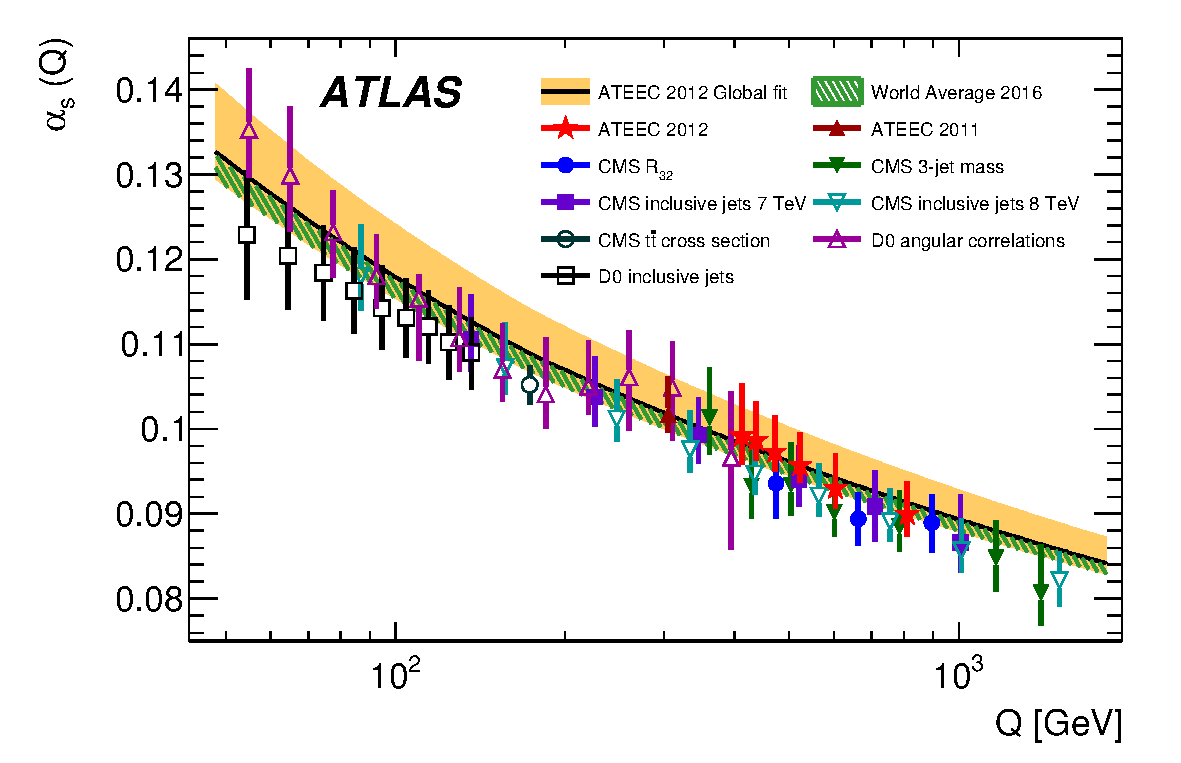
\includegraphics[width=0.8\textwidth]{figures/springer/strong_coupling.pdf}
\caption{Experimental determinations of the \gls{qcd} coupling constant $\alpha_\mathrm{s}$. 
The 2016 world average  is shown in the green hatched band. 
Figure from Ref \cite{Aaboud_2017_alpha}.}
\label{fig:sm:alphas}
\end{figure}

\subsection{Electroweak interaction and Higgs-Englert-Brout mechanism}
\label{sec:smsusy:ew}

The theory of electroweak interactions is based on the symmetry group $SU(2)_\mathrm{L} \times U(1)_\mathrm{Y}$. This symmetry breaks at a scale around 100 GeV giving rise to the electromagnetic interaction, mediated by the photon, and to the weak interaction, mediated by the $Z$ and $W^{\pm}$ bosons  for neutral currents and charged currents respectively. The number of mediators, four, is the same as the number of generators of the symmetry group. 

The $SU(2)_\mathrm{L}$ part of the symmetry group governs the weak interactions, and the subscript L indicates that only left-handed particles participate to them. Left-handed and right-handed fields ($\psi_L$ and $\psi_R$ respectively) are defined through the chirality projectors $P_L$ and $P_R$:

\begin{equation}
\begin{aligned}
\psi_L = P_L \psi = \frac{(1 - \gamma_5)}{2} \psi \; , \\
\psi_R = P_R \psi = \frac{(1 + \gamma_5)}{2} \psi \; , \nonumber
\end{aligned}
\label{eq:sm:LR}
\end{equation}

\noindent where $\gamma_5$ is defined as $\gamma_5 = i \gamma^0 \gamma^1 \gamma^2 \gamma^3 $. Looking back at Equation \ref{eq:sm:dirac}, it can be noted that, if we decompose the fermion field into its left-handed and right-handed components, the derivative term keeps $\psi_L$ and $\psi_R$ separated, while the mass term mixes them:
\begin{equation}
-m \bar \psi \psi = -m \bar \psi P_L^2 \psi - m \bar \psi P_R^2 \psi
	= -m \bar \psi_R \psi_L - m \bar \psi_L \psi_R \; .  \nonumber
\end{equation}


\noindent The covariant derivative for the  $SU(2)_\mathrm{L} \times U(1)_\mathrm{Y}$ group is:
\begin{equation}
\mathcal{D}_{\mu} = \partial_{\mu} - i g' B_\mu Y - ig W_\mu^k T^k \; ,
\label{eq:sm:covD}
\end{equation}

\noindent and substituting with this the regular derivative results in the interaction Lagrangian:
\begin{equation}
\mathcal{L}_{int}^{EW} = -\frac{g'}{2} \left( \bar{\psi} \gamma_\mu Y \psi \right) B^\mu - g \sum_k \left( \bar{\psi} \gamma_\mu T^k \psi  \right) W_k^\mu \; , \nonumber
\end{equation}

\noindent where we have introduced $T^k$, the weak isospin operator, and $Y$, the hypercharge operator (associated to the $U(1)_\mathrm{Y}$ group), and the respective coupling constants $g$ and $g'$. The quantum numbers of the $T^k$ and $Y$ operators relate to the electric charge $Q$ through the  Gell-Mann Nishijima relation:

\begin{equation}
Q = \frac{Y}{2} + T_3 \; , \nonumber
\label{eq:sm:Q}
\end{equation}

\noindent where $Y$ is the hypercharge quantum number and $T_3$ is the quantum number of the third component of the isospin. 

In the case of an $SU(2)$ symmetry, it is not possible to add directly to the Lagrangian a mass term for the vector bosons of the form in Equation \ref{eq:lproca}, as it would spoil the $SU(2)$ local invariance. The Higgs-Englert-Brout mechanism \cite{Englert:1964et, Higgs:1964pj, Higgs:1964ia} solves this problem through \gls{ssb} of the $SU(2)_\mathrm{L} \times U(1)_\mathrm{Y}$ invariance. The \gls{ssb} is obtained by adding to the theory one extra isospin doublet of complex scalar components, the Higgs field:

\begin{equation}
	\Phi = \left( \begin{array}{c} \phi^+  \\ \phi^0 \end{array} \right) \; . \nonumber
\end{equation}

\noindent This doublet has hypercharge $Y=1$ and isospin $T=\frac{1}{2}$; the first component has positive electric charge, while the second one is electrically neutral. The Lagrangian for this new field includes a kinetic and a potential term:

\begin{equation}
	\mathcal{L}_{\Phi} = ( \mathcal{D}_{\mu} \Phi)^{\dagger} (\mathcal{D}^{\mu} \Phi) - V(\Phi) \; ,
	\label{eq:LHiggs}
\end{equation}

\noindent where $\mathcal{D}_{\mu}$ is the covariant derivative defined in Equation \ref{eq:sm:covD} and the potential $V(\Phi)$ is given by:

\begin{equation}
 V(\Phi) =  \mu^2 \Phi^{\dagger} \Phi + \lambda (\Phi^{\dagger} \Phi)^2 \, . \nonumber
	\label{eq:hpot}
\end{equation}

\noindent The two real parameters $\mu^2$ and $\lambda$ relate respectively to the mass term and the strength of the self-interaction term. The shape of the potential depends on the value of these parameters:
\begin{itemize}
\item If $\lambda < 0$, the potential does not present any stable minima, and this case is therefore unphysical.
\item If $\lambda > 0$ and $\mu^2 > 0$ there is only one solution to the minimization of the potential, $\Phi=0$. This case is shown in Figure  \ref{fig:sm:HiggsV_1}.
\item If $\lambda > 0$ and $\mu^2 < 0$, the field acquires a \gls{vev} as the minima is not at zero; it lies instead on the points of the circumference such that:
\begin{equation}
\Phi^{\dagger} \Phi = \frac{\mu^2}{2 \lambda}  \equiv \frac{v^2}{2} \; .
\end{equation}
\noindent Figure \ref{fig:sm:HiggsV_2} illustrates this case.
\end{itemize}


\begin{figure}[ht]
\centering
\subfigure[]{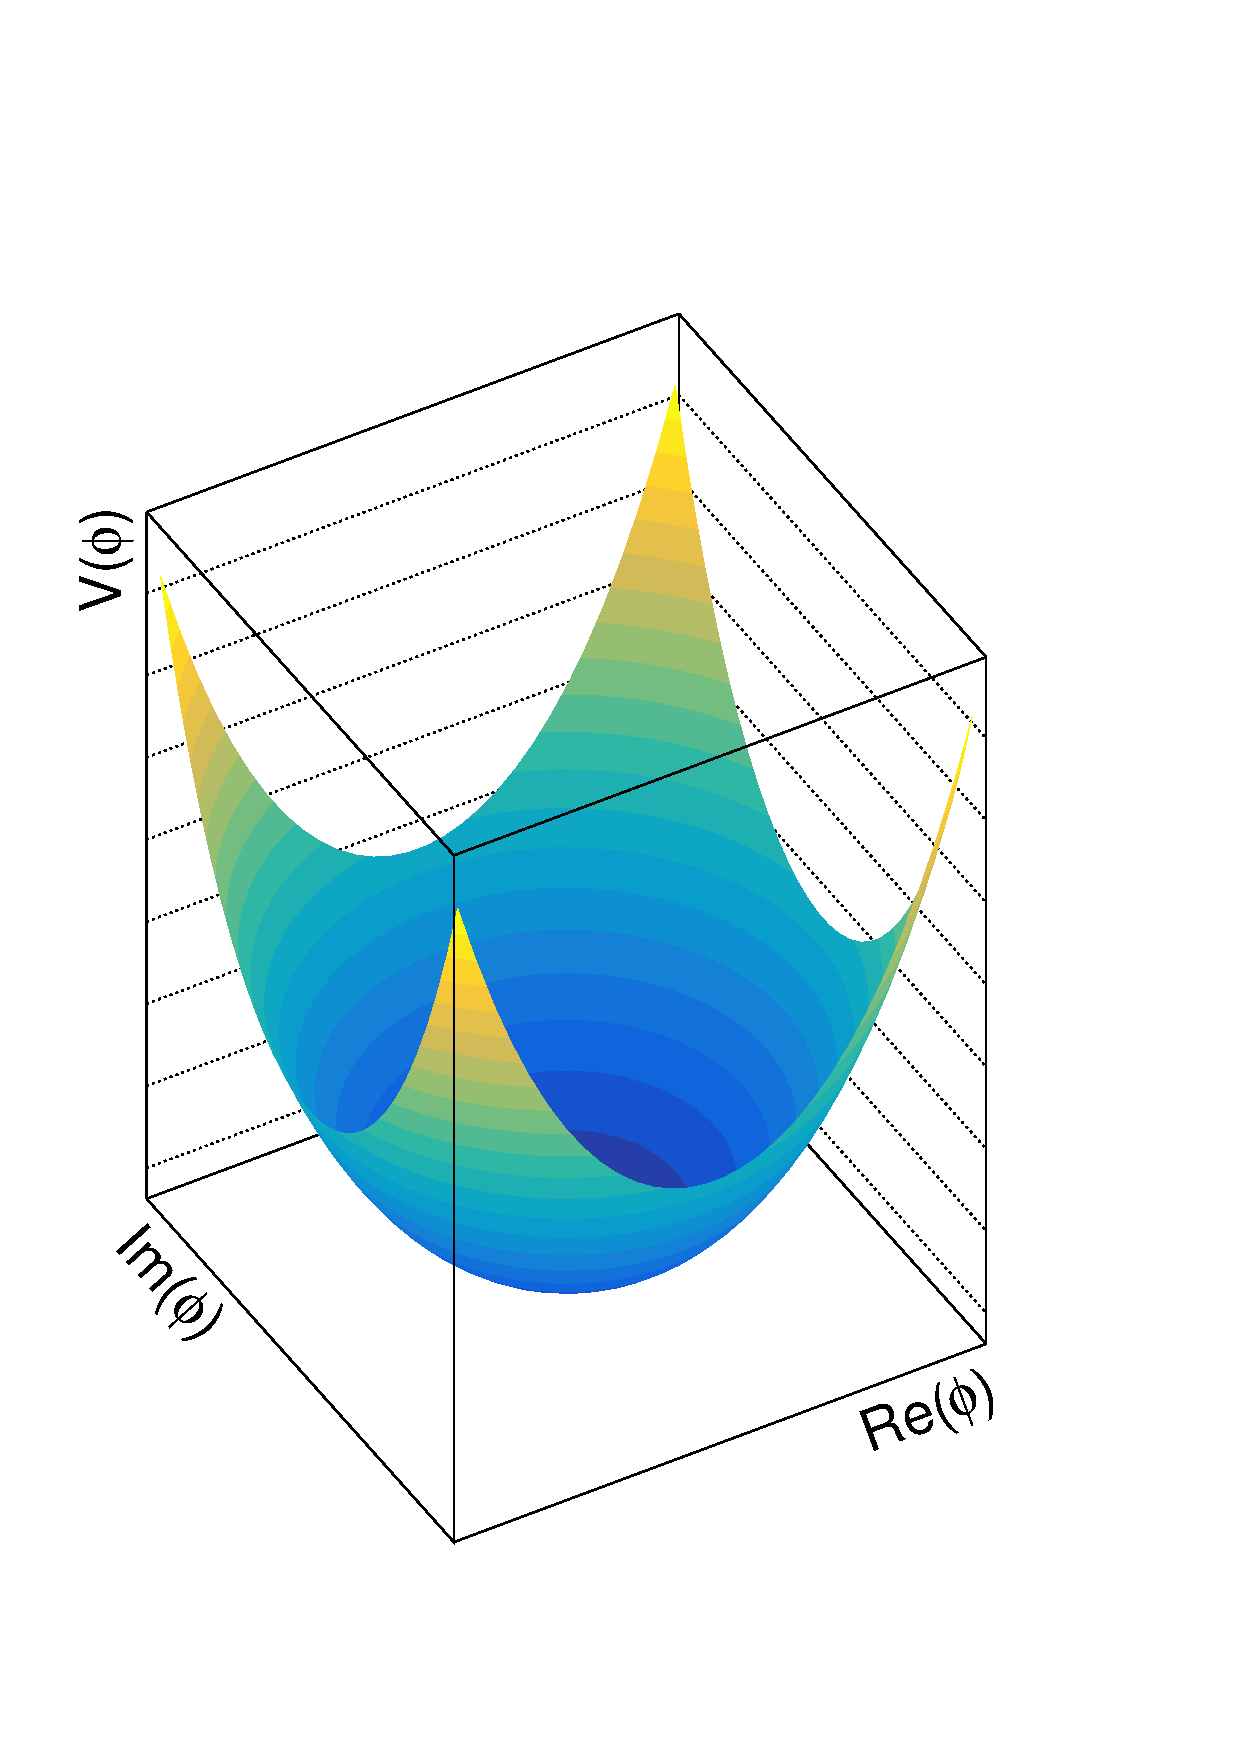
\includegraphics[width=0.49\textwidth]{produce_plots/sm/higgs_posmu2.pdf}\label{fig:sm:HiggsV_1}}
\subfigure[]{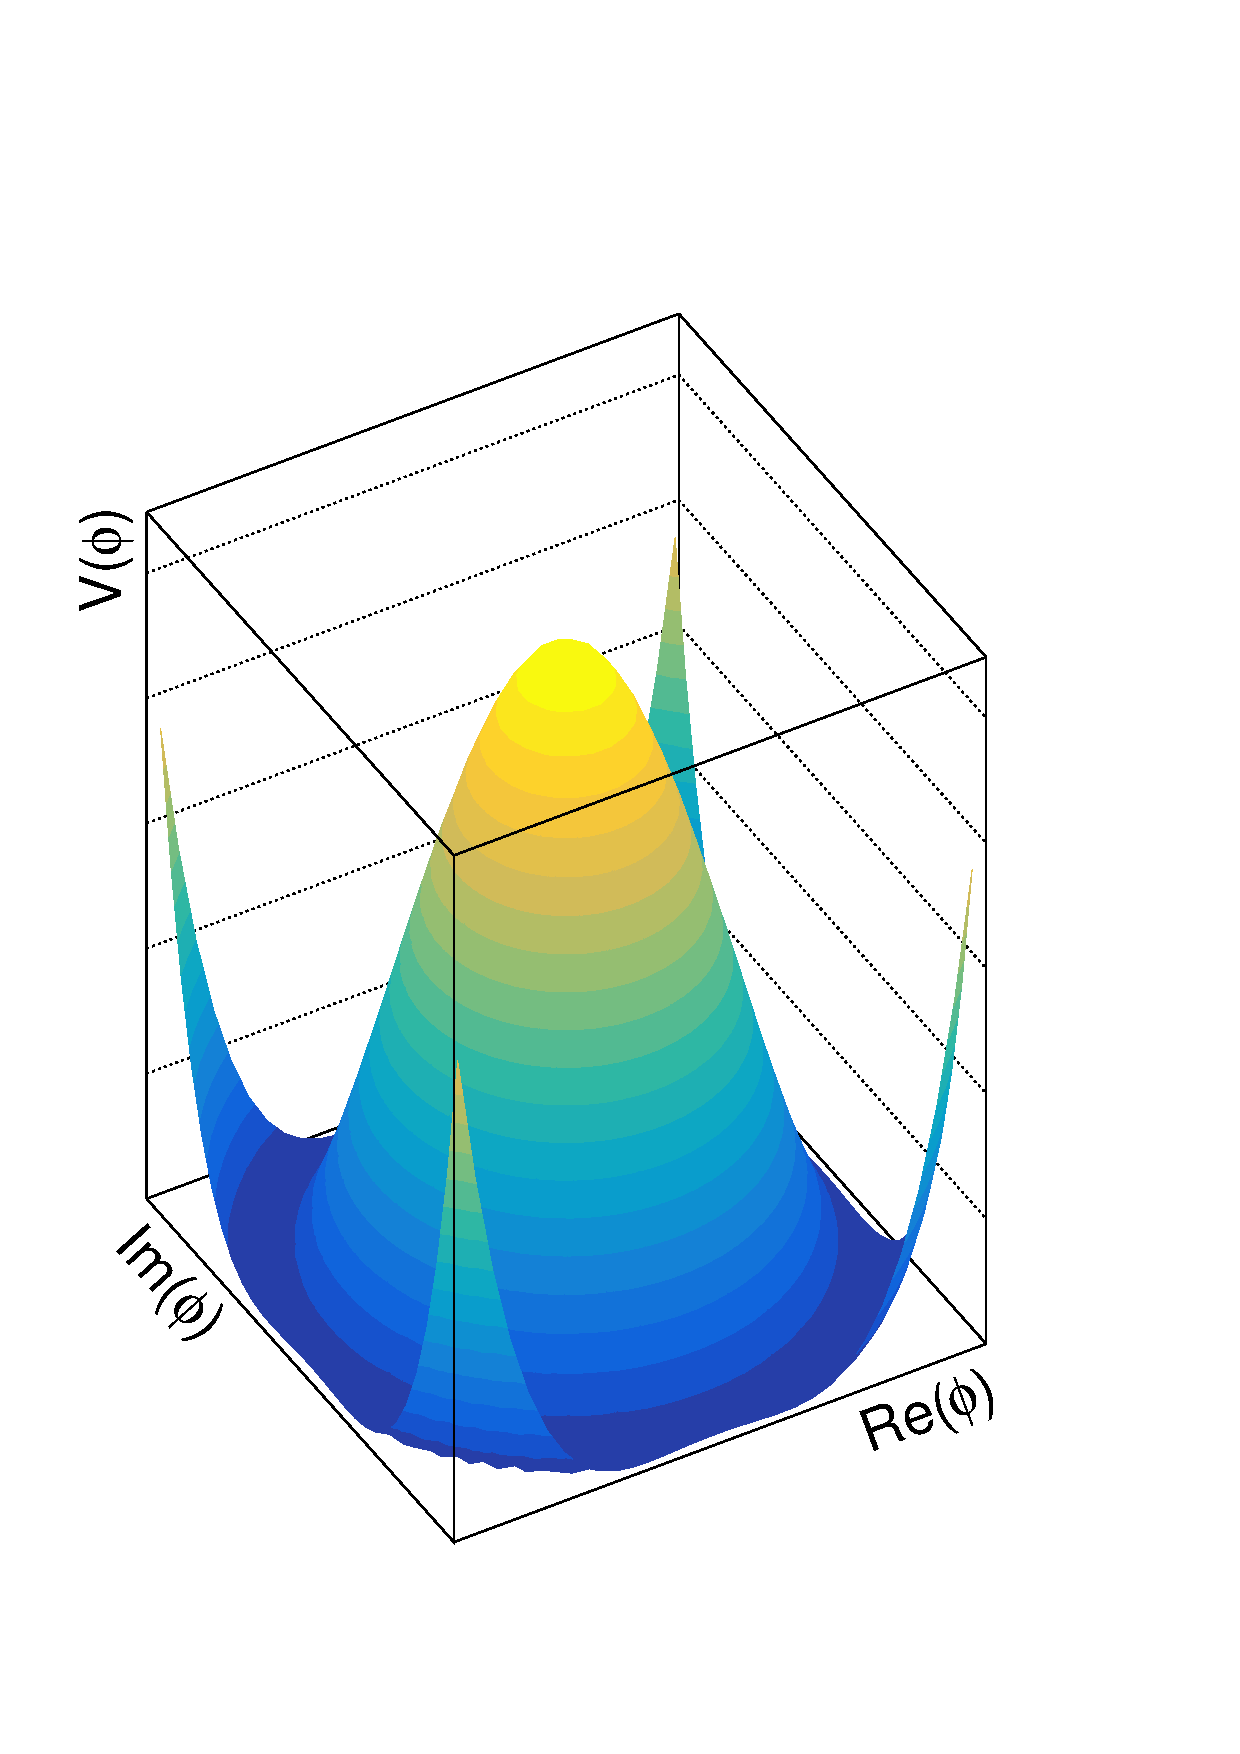
\includegraphics[width=0.49\textwidth]{produce_plots/sm/higgs_negmu2.pdf}\label{fig:sm:HiggsV_2}}
\caption{Higgs potential in the case \subref{fig:sm:HiggsV_1} $\lambda > 0$ and  $\mu^2 > 0$ and \subref{fig:sm:HiggsV_2} $\lambda > 0$ and $\mu^2 < 0$.}
\label{fig:sm:HiggsV}
\end{figure}

Up to this point the $SU(2)_\mathrm{L} \times U(1)_\mathrm{Y}$ symmetry is still intact, but the explicit choice of one of the infinite possible vacuum states for the Higgs field breaks the symmetry. According to the Goldstone theorem \cite{Goldstone:1962es}, the breaking of a continuous symmetry leads to the appearance of new massless scalar particles as field excitations. These new degrees of freedom are absorbed by the existing gauge bosons, thus giving them mass. To meet the experimental requirement of a massless photon, the choice of the Higgs vacuum has not to break the electromagnetic symmetry, $U(1)_{EM}$, so the component of the Higgs doublet that acquires a \gls{vev} is the neutral one:

\begin{equation}
	\Phi_0 = \frac{1}{\sqrt{2}} \left( \begin{array}{c} 0 \\ v  \end{array} \right) \, . \nonumber
\label{eq:hvphi}
\end{equation}

We can then expand the field $\Phi$ considering small excitations around the minimum:

\begin{equation}
	\Phi = \frac{e^{i \vec{\sigma} \cdot \vec{\theta}(x)/v }}{\sqrt{2}} \left( \begin{array}{c} 0 \\ v + \phi(x) \end{array} \right) \, ,
\label{eq:hvphi}
\end{equation}

\noindent where $\phi(x)$ is the physical field associated with the Higgs boson, $\vec{\sigma}$ the Pauli matrices and $\vec{\theta}(x)$ the three degrees of freedom absorbed to give masses to the $Z$ and $W^\pm$ bosons. Inserting Equation \ref{eq:hvphi} into Equation \ref{eq:LHiggs} relates the mass of the Higgs boson to the parameters in the potential:
\begin{equation}
m_H = \sqrt{- 2 \mu^2} = \sqrt{2 \lambda} v \; .
\label{eq:sm:Higgsmass}
\end{equation}

Since the numeric value of the $\mu^2$ and $\lambda$ parameters is not set, the theory does not predict a specific value for $m_H$. 
The physical mass eigenstates of the gauge bosons are a rotation of the interaction eigenstates, given by:

\begin{equation}
\begin{aligned}
W_\mu^\pm &= \frac{W_\mu^1 \mp W_\mu^2}{\sqrt{2}} \; , \\
A_\mu &= B_\mu \cos\theta_W + W^3_\mu \sin\theta_W \; ,  \\
Z_\mu &= W^3_\mu \cos\theta_W - B_\mu \sin\theta_W \; , \nonumber
\end{aligned}
\label{eq:wein}
\end{equation}

\noindent where we have introduced the Weinberg angle $\theta_W$ such that:
\begin{equation}
\tan\theta_W \equiv \frac{g'}{g} \; . \nonumber
\end{equation}


The $(\mathcal{D}_{\mu} \Phi)^{\dagger} (\mathcal{D}^{\mu} \Phi)$ term in Equation \ref{eq:LHiggs} gives rise to the physical mass of the gauge bosons: once applied to the Higgs field, the covariant derivative in Equation \ref{eq:sm:covD} produces terms quadratic in the gauge fields, that we interpret as mass terms:

\begin{equation}
\mathcal{L}_{\Phi} = \left(1+\frac{\phi}{v}\right)^2 \,
\left\{ m_W^2\, W_\mu^\dagger W^\mu
+ \frac{1}{2}\, m_Z^2\, Z_\mu Z^\mu \right\}\, +\, \mathcal{L}_H \; ,  \nonumber
\end{equation}

\noindent where $\mathcal{L}_H$ denotes all the terms in $\mathcal{L}_{\Phi}$ that involve only the Higgs field: Higgs boson mass, cubic and quadratic self-interaction. Note that the coupling of the gauge bosons with the Higgs field is proportional to the square of the boson mass.
At tree level the resulting masses of the gauge bosons are:

\begin{equation}
\begin{aligned}
m_\gamma &= 0 \; ,\\
m_Z &= \frac{v \sqrt{g^2 + g'^2}}{2} \; , \\
m_W &= \frac{vg}{2} =  \cos\theta_W m_Z \; . \nonumber
\end{aligned}
\end{equation}


Therefore, the Higgs-Englert-Brout mechanism generates automatically a mass term for the gauge bosons, that does not break the global underlying $SU(2)_\mathrm{L} \times U(1)_\mathrm{Y}$ symmetry. The Higgs field is also used to make fermion mass terms arise, but in this case it is necessary to postulate a Yukawa interaction between the Higgs and fermion fields. The fermion masses are assumed to be proportional to the strength of the coupling and, unlike the masses of the gauge bosons, they are not related to other parameters of the theory. While the Higgs field itself is enough to give mass to down-type fermions, the mass term for the up-type fermions  requires the introduction of the complex conjugate of the Higgs field ($\Phi_C$):

\begin{equation}
 \Phi_C = i \sigma^2 \Phi^* 
	= i \left( \begin{array}{cc} 0 & -i \\ i & 0 \end{array} \right) 
	\left( \begin{array}{c} \phi^- \\ \phi^{0*} \end{array} \right)
	= \left( \begin{array}{c} \phi^{0*} \\ - \phi^- \end{array} \right) \; . \nonumber
\end{equation}

\noindent If we identify as $y_f$ the coupling of the fermion $f$ to the Higgs field, referred to as Yukawa coupling, the additional part of the Lagrangian that generates the fermion masses is:

\begin{equation}
\begin{aligned}
\mathcal{L}_{Yukawa} &= - \left[  y_d \left( \bar{u}_L \,\, \bar{d}_L  \right) \Phi d_R +  y_u \left( \bar{u}_L \,\, \bar{d}_L  \right) \Phi_C u_R \right] + h.c. \\
&= - \frac{1}{\sqrt{2}} \left[  y_d \left( v + \phi \right) \bar{d}_L d_R + h.c. + y_u \left( v + \phi \right) \bar{u}_L d_u + h.c. \right]  \; . \nonumber
\end{aligned} 
\end{equation}

\noindent In this equation we can now easily identify the fermion mass terms, of the form:

\begin{equation}
m_f =  \frac{v}{\sqrt{2}} y_f \; . \nonumber
\end{equation}

\noindent Note that, in the case of fermions, the coupling to the Higgs boson is directly proportional to the fermion mass. 
The matrices $y_f$ are not necessarily diagonal, but they can be diagonalized through a unitary transformation, which we can interpret as the transformation that relates the mass eigenstates to the weak interaction eigenstates. In the quark sector, this transformation is encoded in the \gls{ckm} matrix \cite{Cabibbo:1963yz, Kobayashi:1973fv}, that describes the mixing of the down-type quarks. In the \gls{sm} with three generations of fermions, the \gls{ckm} matrix is parametrized by three angles and one complex phase that provides the only source of CP violation.

\subsection{Measured properties of the Higgs boson}

The value of the Higgs boson mass is not predicted by the \gls{sm}, but it can be measured and, once it is know, the Higgs boson production cross-section and decay fractions can be predicted accurately. These predictions can be verified experimentally, supporting the idea that the discovered boson is indeed the \gls{sm} Higgs boson. In 2015 the ATLAS and CMS collaborations published a combined measurement of the Higgs boson mass \cite{Aad:2015zhl}:
\begin{equation}
m_H = 125.09 \pm 0.21 (\mathrm{stat.}) \pm 0.11 (\mathrm{syst.}) \;\; \mathrm{GeV}. \nonumber
\end{equation}

\noindent This result uses the full Run 1 ATLAS and CMS data, analyzed in the $h \rightarrow \gamma \gamma$ and $h \rightarrow ZZ^{*} \rightarrow 4 \; \mathrm{leptons}$ channels.


The discussion of the Higgs mechanism in Section \ref{sec:smsusy:ew} highlights interesting properties of the interactions involving the Higgs boson. In particular, the strength of its coupling with fermions and bosons is proportional respectively to the mass and the square of the mass of the particle involved. 
This is reflected on the \glspl{br}: they are high for the decay to particles with the highest mass that are kinematically allowed.
While the top quark mass is too large for the decay $h \to t\bar{t}$ to exist, the large top Yukawa coupling leads to loop-induced couplings of the Higgs boson to massless particles (gluons and photons); these are of phenomenological interest as they lead to the main production mode (gluon-gluon fusion) and to the $h \to \gamma \gamma$ decay mode, which has a low \gls{br} but leads to a very clean signature and was one of the key channels for the Higgs boson discovery. 
The theoretical production cross-section and \glspl{br} for a Higgs boson with mass between 120 and 130 GeV are reported in Figure \ref{fig:sm:h_xsec_br}.

\begin{figure}[ht]
\centering
\subfigure[]{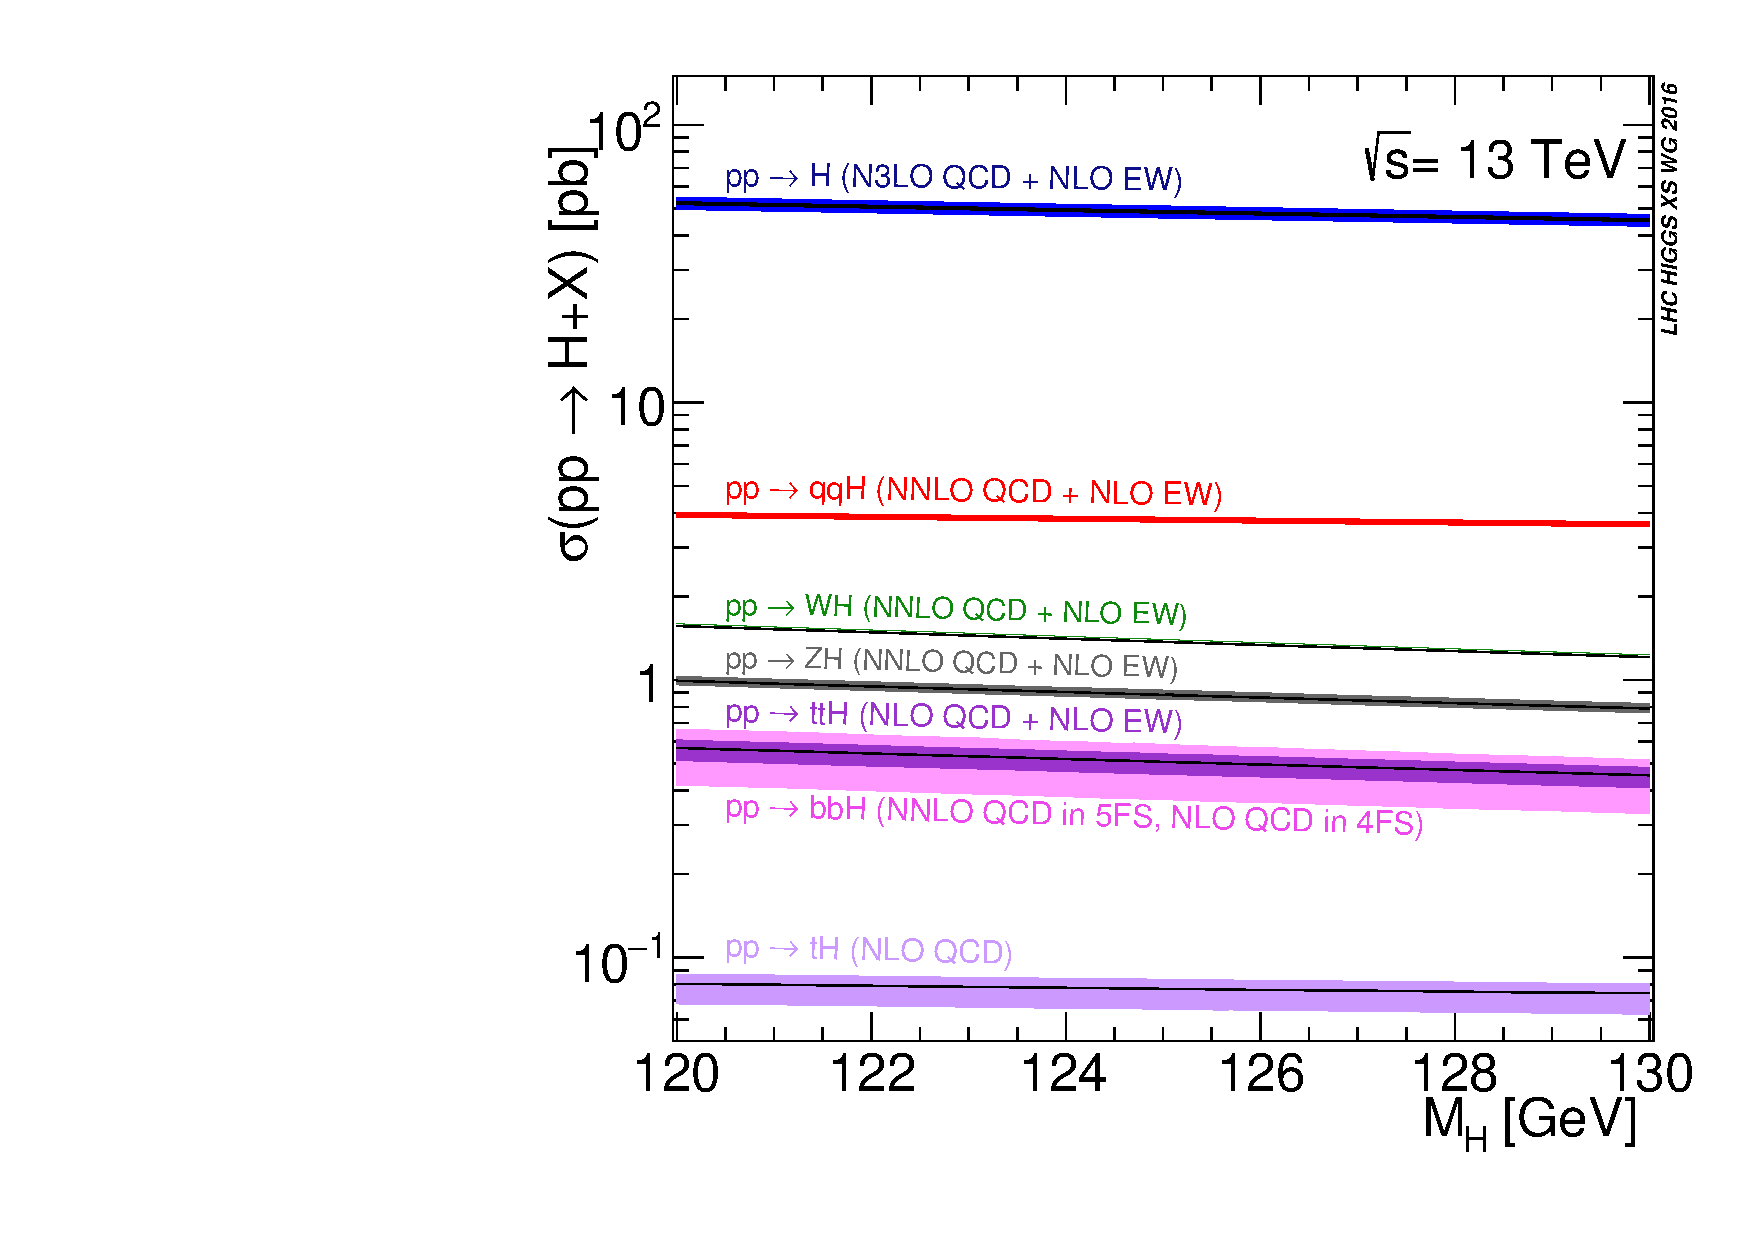
\includegraphics[width=0.49\textwidth]{figures/theory/plot_13tev_H_sqrt}\label{fig:sm:h_xsec_theo}}
\subfigure[]{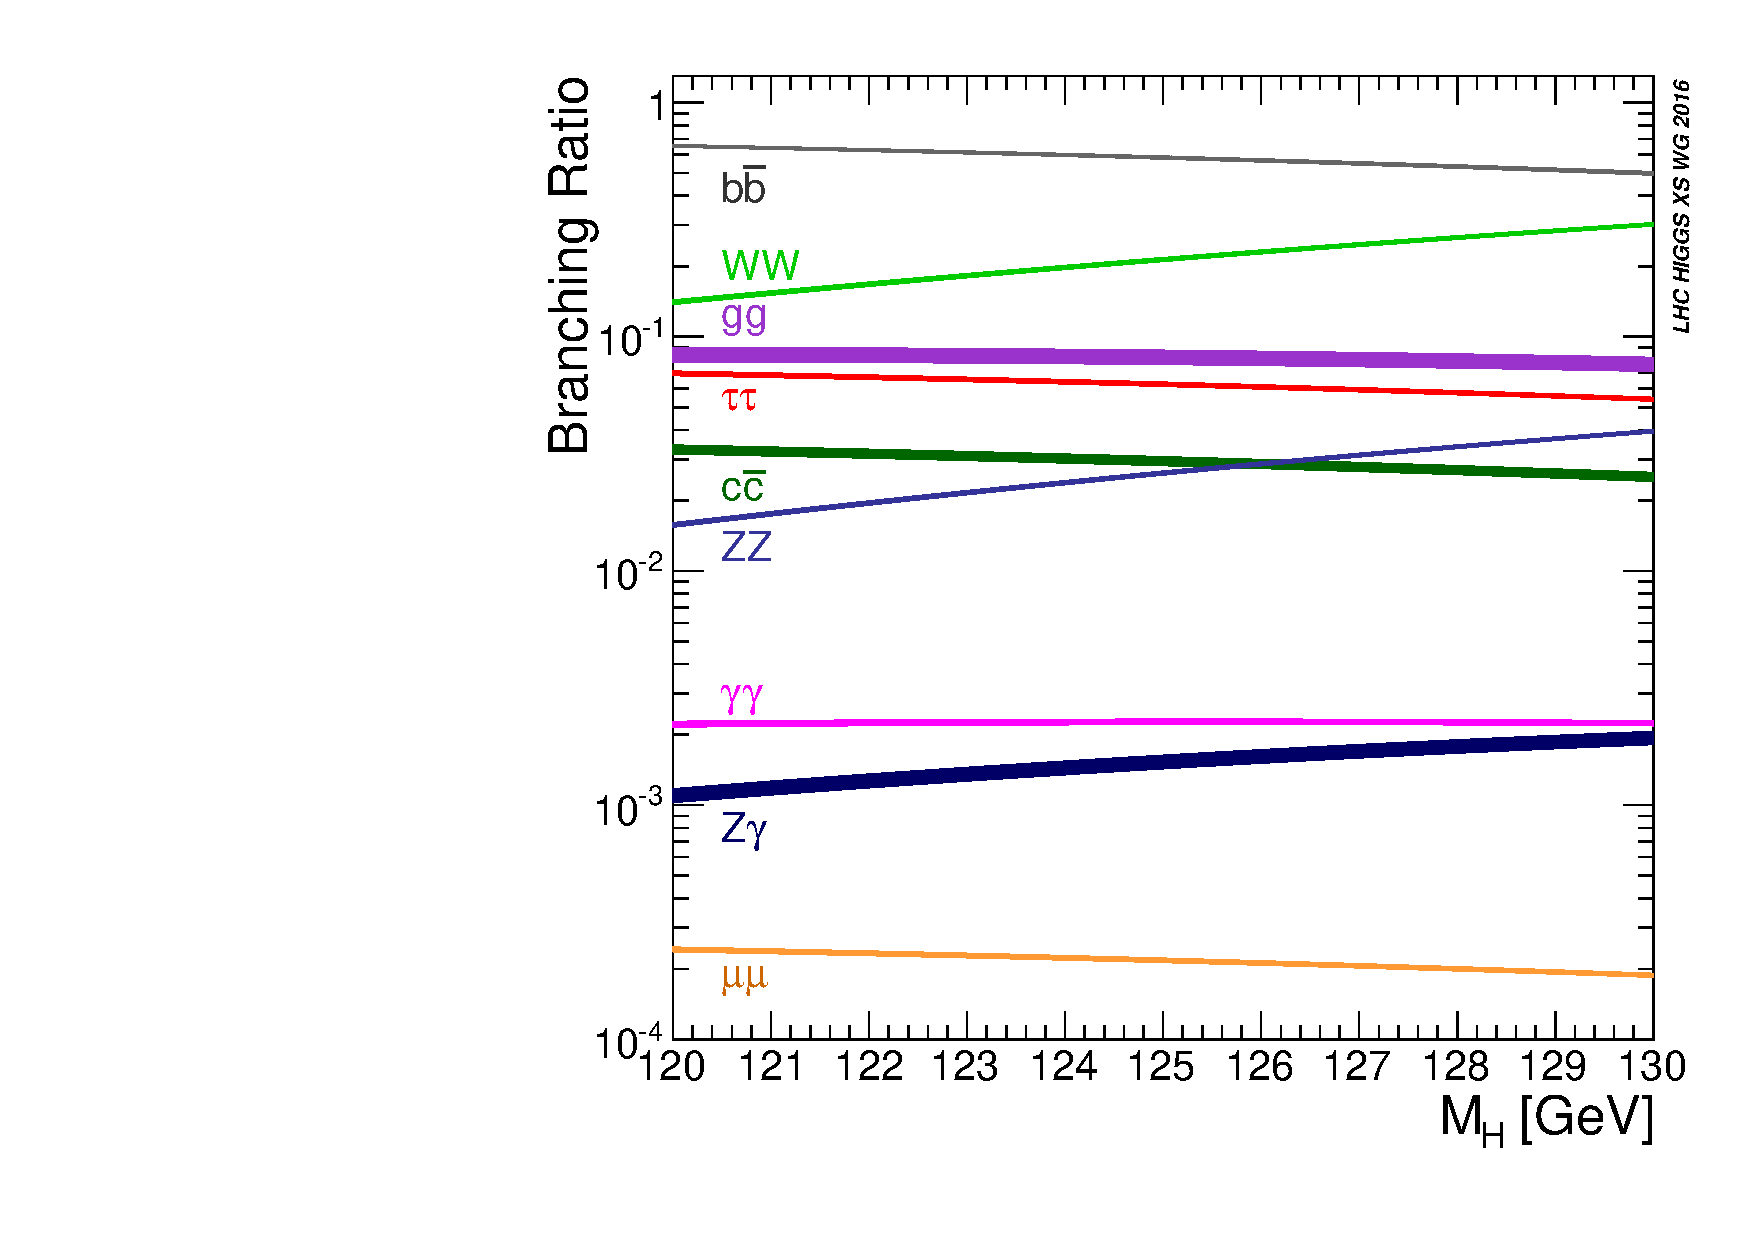
\includegraphics[width=0.49\textwidth]{figures/theory/SMHiggsBR_120-130.pdf}\label{fig:sm:h_br_theo}}
\caption{
\subref{fig:sm:h_xsec_theo} Higgs boson production cross-section at 13 TeV for a mass range between 120 and 130 GeV.
\subref{fig:sm:h_br_theo} Higgs boson \gls{br} for a mass range between 120 and 130 GeV.
Figures from Ref.  \cite{deFlorian:2016spz}.}
\label{fig:sm:h_xsec_br}
\end{figure}

The production cross-section is found to be in agreement with the \gls{sm} predictions within uncertainties. Figure \ref{fig:sm:h_xsec} shows the best fit value of Higgs production cross-section times \gls{br} in the different production and decay modes \cite{Khachatryan:2016vau}. Also the relation between the fermion or boson mass and the Higgs coupling has been verified experimentally, as show in Figure \ref{fig:sm:h_mass}. 

\begin{figure}[ht]
\centering
\subfigure[]{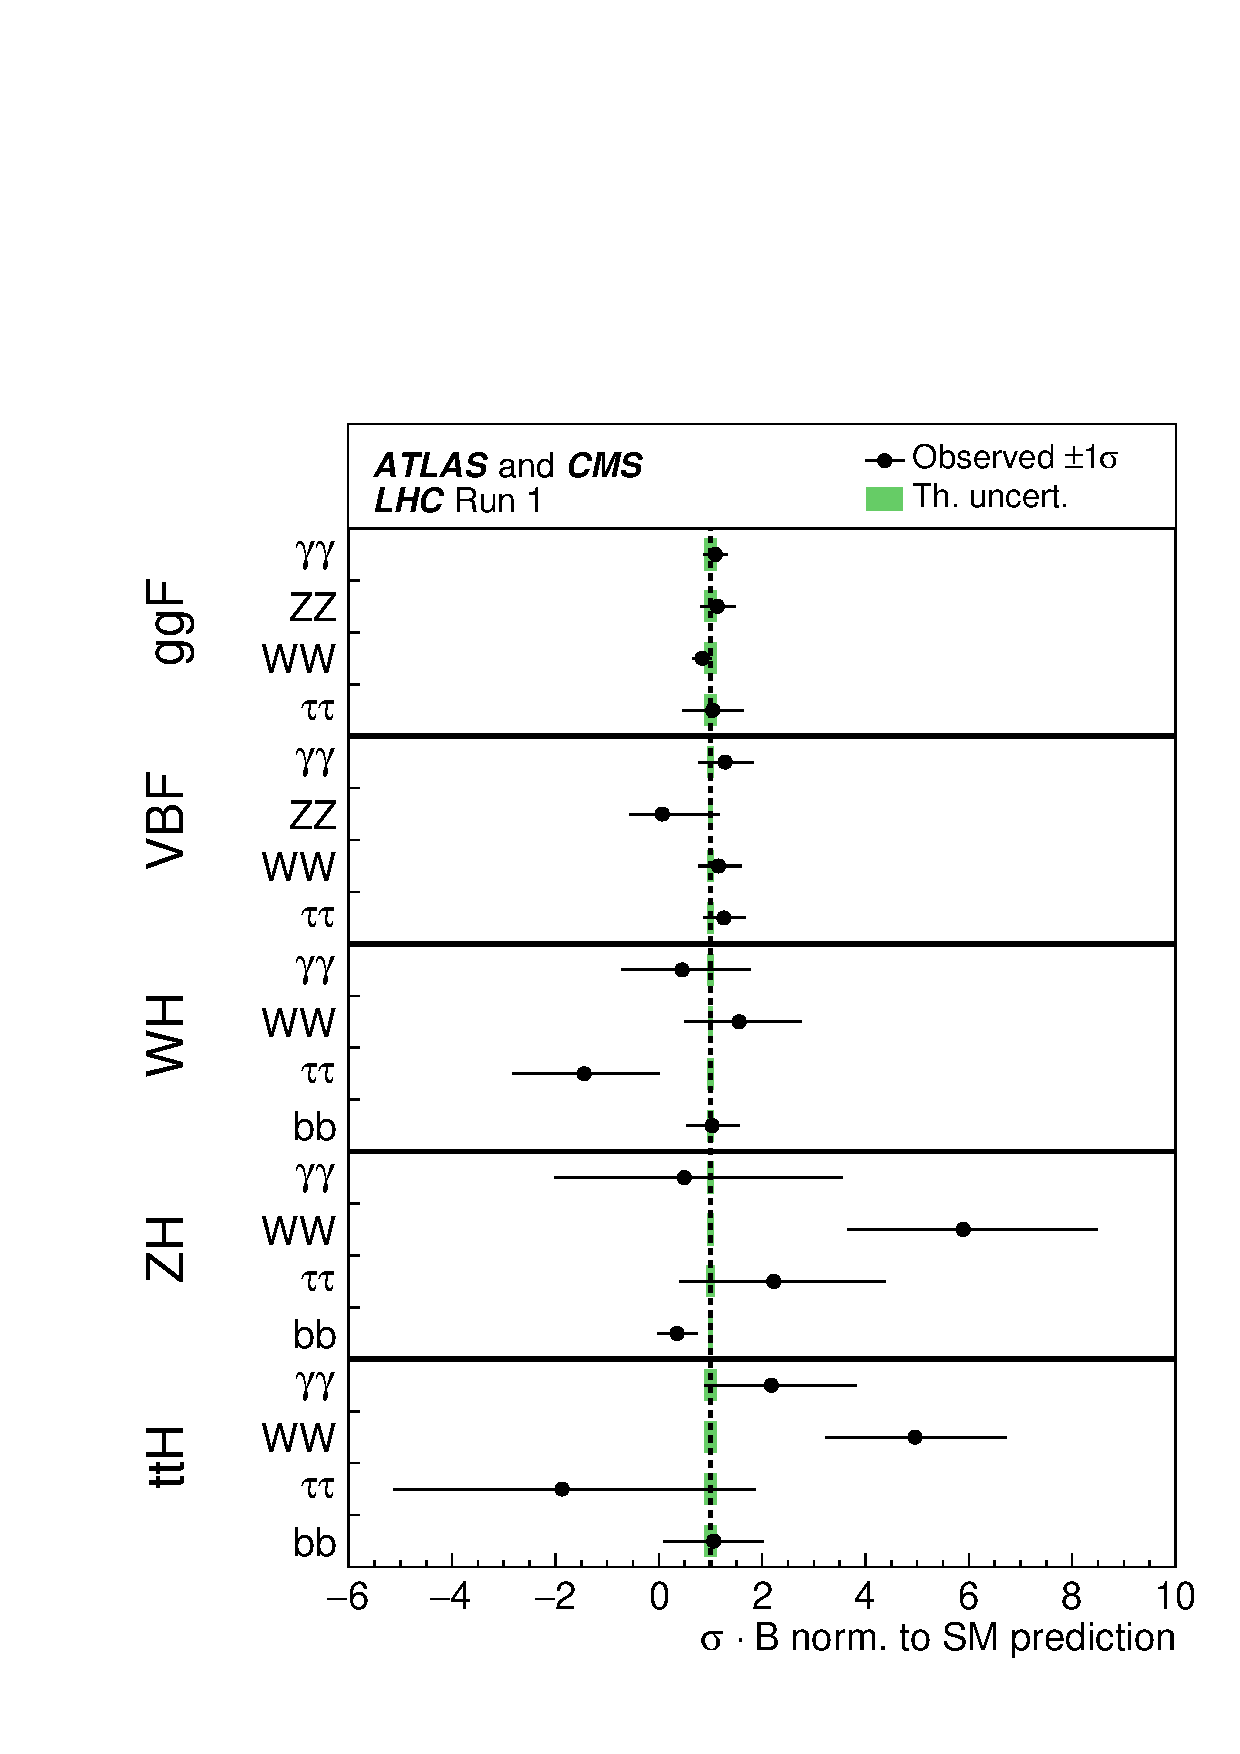
\includegraphics[width=0.49\textwidth]{figures/theory/CMS-HIG-15-002_Figure_007}\label{fig:sm:h_xsec}}
\subfigure[]{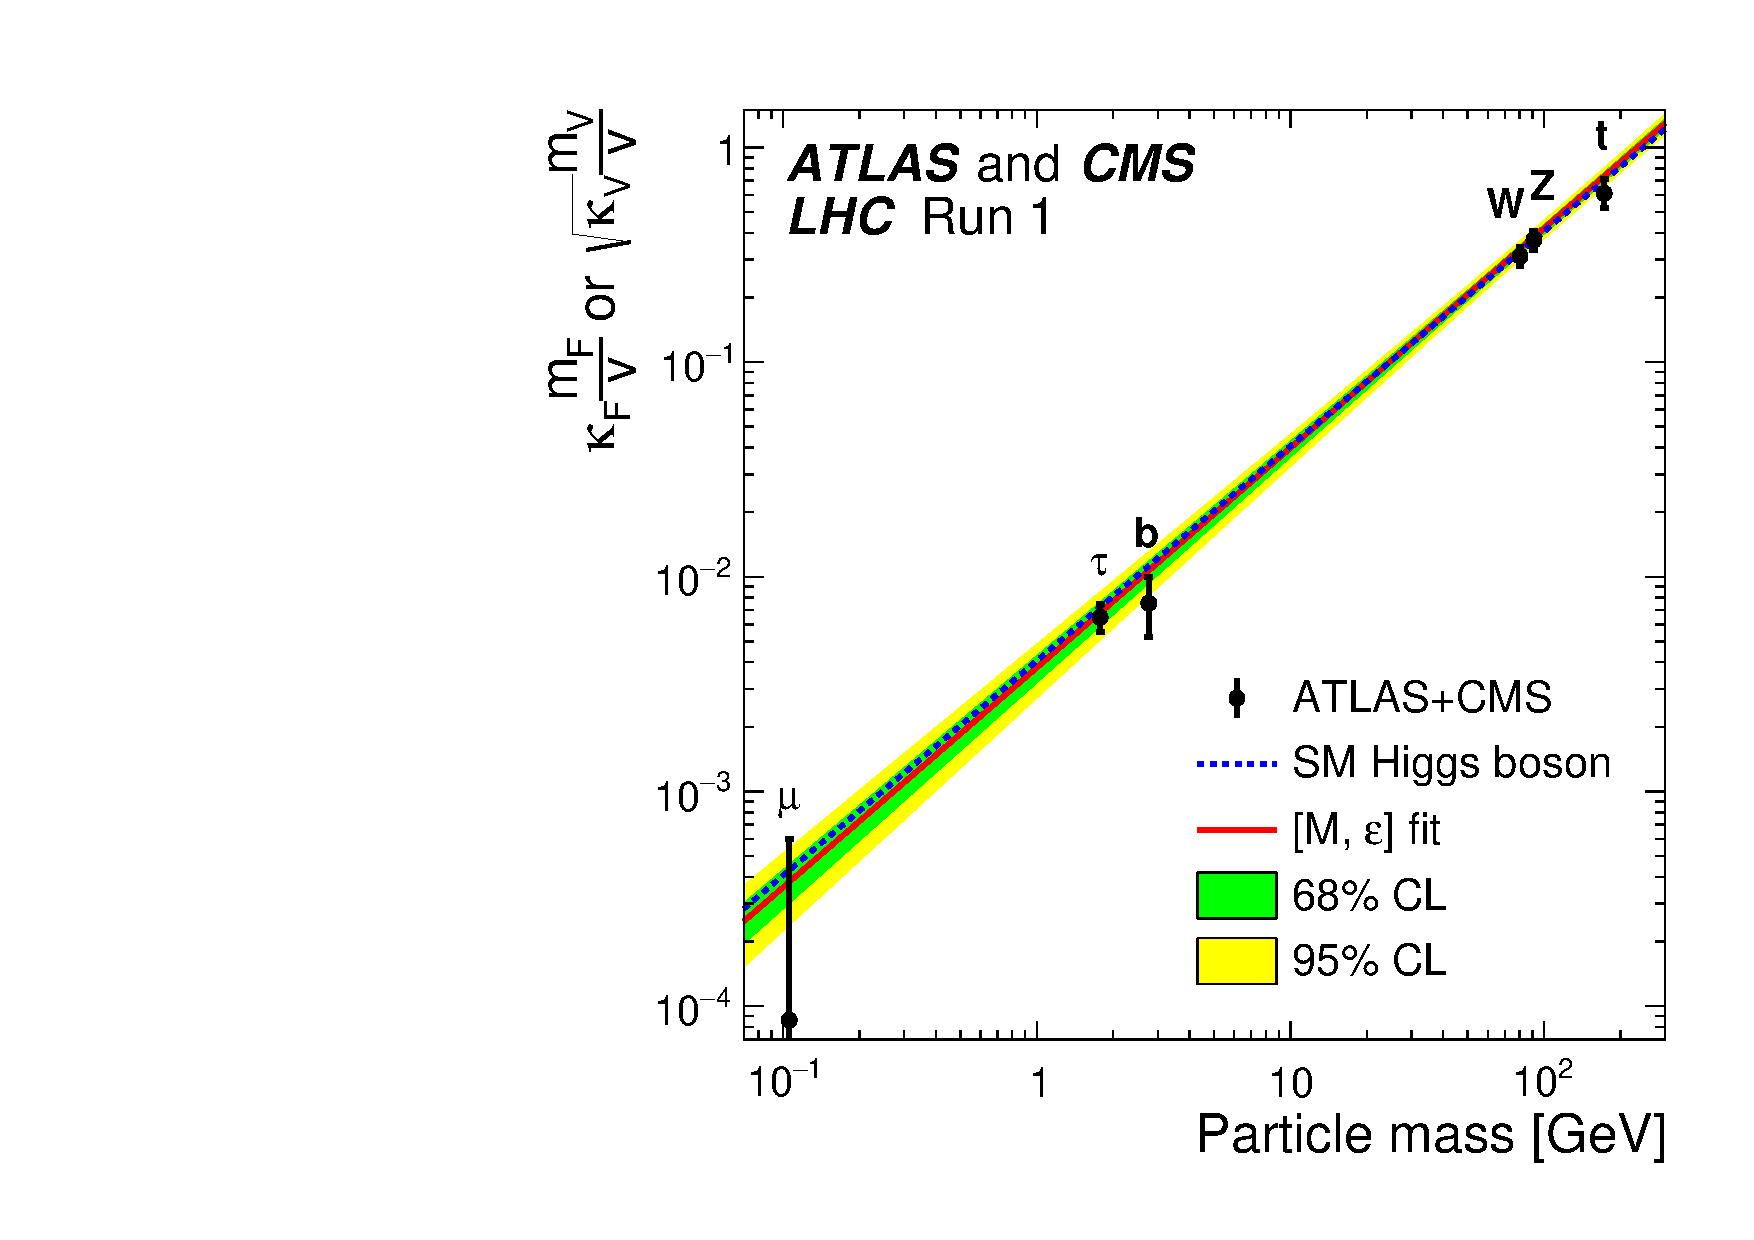
\includegraphics[width=0.49\textwidth]{figures/theory/CMS-HIG-15-002_Figure_019}\label{fig:sm:h_mass}}
\caption{
\subref{fig:sm:h_xsec} Best-fit value of Higgs production cross-section times \gls{br} in different production and decay modes. 
\subref{fig:sm:h_mass} Best-fit values as a function of particle mass for the combination of Run 1 ATLAS and CMS data. 
Figures from Ref.  \cite{Khachatryan:2016vau}. 
}
\label{fig:sm:h_couplings_mass}
\end{figure}

 


\section{Limitations of the Standard Model and how to extend it}
\label{sec:smsusy:bsm}

Despite its undeniable success in describing the subatomic world, the \gls{sm} has some limitations that suggest it should be considered as the low-energy approximation of a more general theory. Nowadays there is no perfect candidate to fill the role of this general theory, but the shortcomings of the \gls{sm} highlight the characteristics this theory should have. Section \ref{sec:sm:missingpieces} discusses the experimental observations that are not accounted by the \gls{sm} framework, whose lacking is an objective limit of the \gls{sm}. In Section \ref{sec:sm:aesthetics} we review some other features that the \gls{sm} is missing that, while not being strictly necessary, would be desirable in a general theory. Some theories and models candidate to extend the \gls{sm} are briefly presented in Section \ref{sec:sm:extensions}.

\subsection{Unexplained phenomena}
\label{sec:sm:missingpieces}

The \gls{sm} lacks an explanation for some well established experimental phenomena that are listed in the next paragraphs.

\subsubsection*{Neutrino Masses}

Neutrino oscillations \cite{PhysRevLett.81.1562} are possible only if there is a mass difference between the three neutrino generations, which automatically implies non-zero masses for at least some neutrinos. Although neutrino mass terms could be accommodated by the \gls{sm} through right-handed neutrinos or a description of neutrinos as Majorana particles, the basic formulation of the \gls{sm} describes neutrinos as massless particles.

\subsubsection*{Dark Matter and Dark Energy}

The \gls{sm} describes only baryonic matter; this accounts for about 5\% of the energy density in the universe. Even though no direct observation of it has been made so far, we know there is also another type of matter, that does not have electromagnetic interactions and  is about five times more abundant than ordinary matter.  Since this type of matter does not reflect light, it is referred to as dark matter. The presence of dark matter has been postulated for the first time from the rotational velocity of galaxies \cite{Zwicky:1937zza}, but this evidence has now been confirmed also by other observations, including the analysis of the cosmic microwave background from the WMAP and Planck collaborations \cite{Larson:2010gs,Ade:2013zuv}. The sum of baryonic and dark matter accounts for about 32\% of the of the energy density in the universe. 
The remaining 68\%, is the energy responsible for the accelerated expansion of the universe, referred to as dark energy. 
While some extensions of the \gls{sm} provide candidates for dark matter, at the moment no theory provides a compelling explanation for dark energy.


\subsubsection*{CP Violation}

CP-violating processes are needed in order to generate the observed asymmetry between the matter and anti-matter content of our universe. While the \gls{sm} provides one source of CP violation with the complex phase in the \gls{ckm} matrix mentioned in Section \ref{sec:smsusy:ew}, this is not enough and additional sources are needed in order to explain the observed asymmetry.

\subsubsection*{Gravity}

Gravity is the only force acting on elementary particles that is not described by the \gls{sm}. In fact, not only is not described by the \gls{sm}, but the simple attempt to quantize gravity through a spin-2  mediator (graviton) leads to a non-renormalizable theory. The strength of gravity is expected to be comparable to that of the other forces at the Planck scale ($\Lambda_{Planck}$, $\approx 10^{19}$ GeV). 

\subsection{Aesthetic shortcomings}
\label{sec:sm:aesthetics}

While the previous section discusses objective shortcomings of the \gls{sm}, there are also some aesthetic criteria that the \gls{sm} does not seem to satisfy. These are mostly based on the concept of naturalness: unless there is a good reason, the parameters of a ``beautiful'' theory should be all of the same order of magnitude, and a theory where instead the parameters are bound to assume very specific and different values (fine tuning) seems ``unnatural''. It is important to notice that this naturalness requirement is subjective, as well as the amount of fine tuning allowed for a theory to be considered natural.


\subsubsection*{Hierarchy Problem}

The expression for the mass of the Higgs boson in Equation \ref{eq:sm:Higgsmass} contains only the tree-level contribution. The proper computation should include the radiative contributions from all the particles that couple with the Higgs boson, directly or indirectly (see below). A fermion, whose Yukawa coupling leads to the interaction $-y_f \phi \bar{f} f$, will produce a correction to the Higgs boson mass with a divergent integral; this can be computed e.g. with a cut-off regularization, and in this case the resulting correction to the Higgs boson mass, shown in Figure  \ref{fig:sm:h_corr_fermion}, is:
\begin{equation}
\Delta m_H^2 \>=\>  
-{|y_f|^2\over 8 \pi^2} \Lambda_{UV}^2 + \mathcal{O}(\ln \Lambda_{UV} ) \; ,
\label{eq:divhf}
\end{equation}

\noindent where $\Lambda_{UV}^2$ is the cut-off scale, identified with the limit of validity of the theory. If we assume that no physics \gls{bsm} is present up to $\Lambda_{Planck}$, having corrections to the mass proportional to $\Lambda_{Planck}$ requires a fine tuning of the parameters of the order of $\frac{m_H}{\Lambda_{Planck}} \approx 10^{-17}$. This is due to the strong hierarchy of the scales involved (hierarchy problem) \cite{Weinberg:1975gm, PhysRevD.20.2619, PhysRevD.14.1667, tHooft:1979rat}. Since the correction to the mass is proportional to the Yukawa coupling of the fermion, it is clear that the most important correction is the one given by the top quark, whose Yukawa coupling is $y_t \approx 1$. 

Despite this, it can still be argued that the appearance of the $\Lambda_{UV}$ divergence is connected more to the regularization scheme rather than to the theory itself. But even in this case, the value of 125 GeV for the Higgs boson mass remains difficult to justify. The \gls{sm} Lagrangian does not have any symmetry that prevents the Higgs boson to couple to new \gls{bsm} particles. If we assume the existence of a complex scalar that couples with the Higgs field through $ -y_S|\phi|^2 |S|^2$, the correction to the Higgs propagator, shown in Figure \ref{fig:sm:h_corr_scalar}, is given by:

\begin{equation}
\Delta m_H^2 \>=\> {y_S\over 16 \pi^2}
\left [\Lambda_{UV}^2 - 2 m_S^2
\> {\rm ln}(\Lambda_{UV}/m_S) + \ldots
\right] \; .
\label{eq:divhs}
\end{equation}

\noindent Beside the first term, proportional to $\Lambda_{UV}^2$, that can be thought as a consequence of the cut-off regularization, we also have a second  term proportional to $m_S^2$. If we assume that \gls{bsm} physics exists and that, since it has not yet been observed, $m_S$ must be large, this contribution drives $m_H$ to high values. A similar argument applies even if the new \gls{bsm} sector and the Higgs field do not couple directly but, for example, share a gauge interaction, which still gives rise to corrections proportional to the particle’s mass through higher order loop diagrams.

\begin{figure}[ht]
\centering
\subfigure[]
{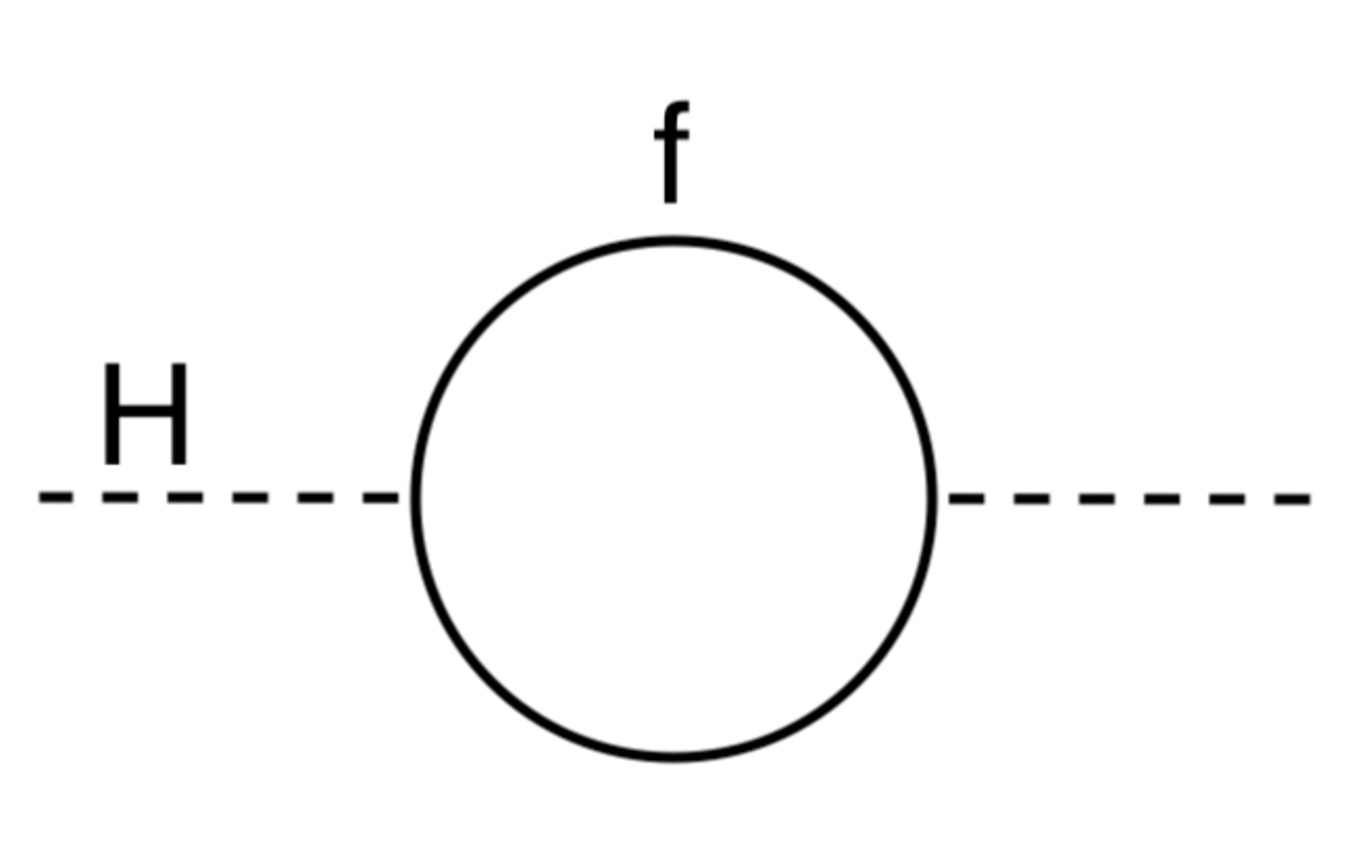
\includegraphics[width=0.36\textwidth]{figures/springer/h_corr_f.pdf}\label{fig:sm:h_corr_fermion}}
\subfigure[]{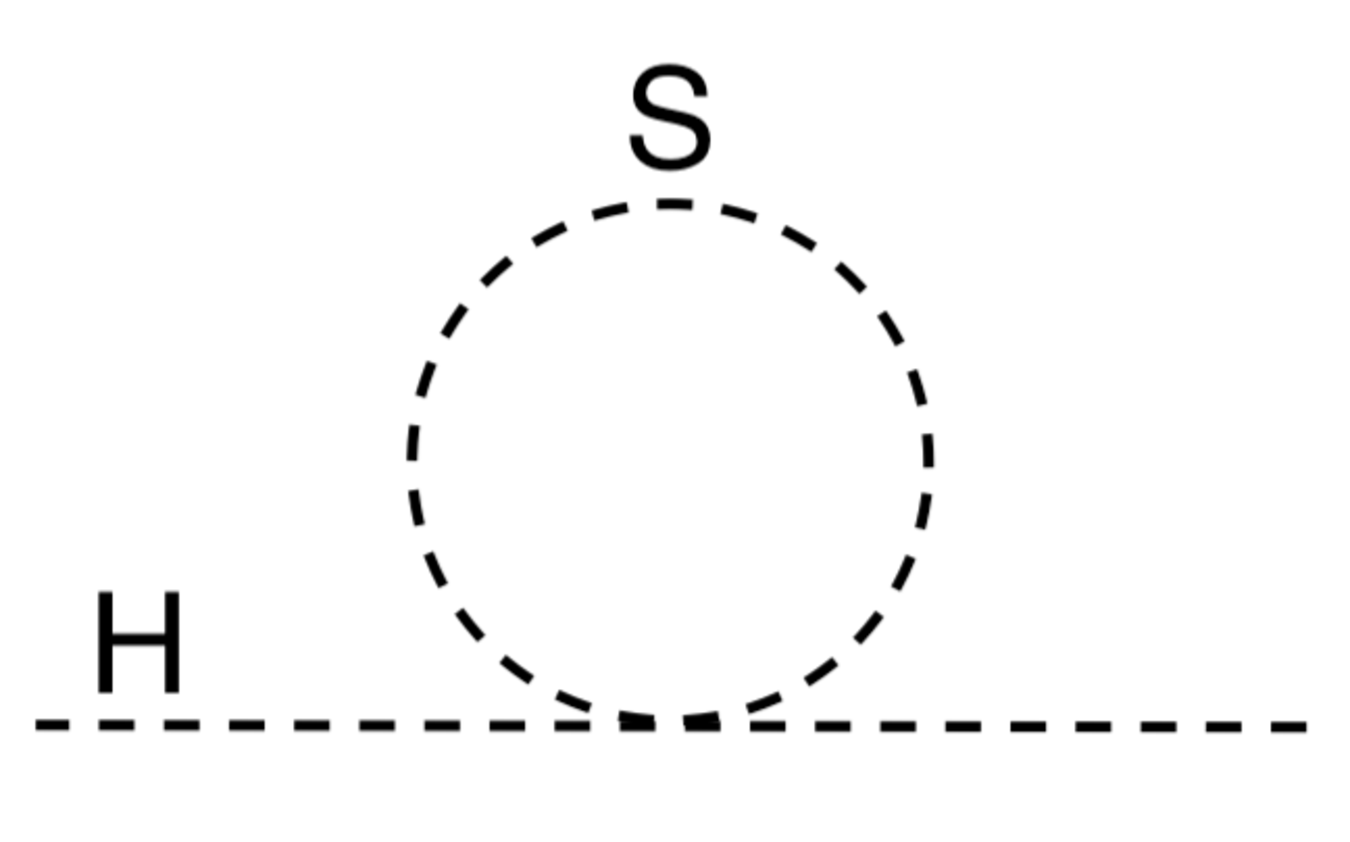
\includegraphics[width=0.36\textwidth]{figures/springer/h_corr_s.pdf}\label{fig:sm:h_corr_scalar}}
\caption{Correction to the Higgs boson propagator form the interaction with \subref{fig:sm:h_corr_fermion} a fermion and \subref{fig:sm:h_corr_scalar} a scalar.}
\label{fig:sm:h_corr}
\end{figure}

\subsubsection*{Fermion Mass Hierarchy} 

Fermion masses are less sensitive than the Higgs boson mass to the cut-off scale as the divergence is only logarithmic. Nevertheless, it is striking how strong the fermion Yukawa coupling hierarchy is: even if we don't consider neutrinos, fermion masses span about six orders of magnitude, without any apparent reason.

\subsubsection*{Unification of Coupling Constants}

The \gls{sm} coupling constants of the $SU(3)_\mathrm{C}$, $SU(2)_\mathrm{L}$ and $U(1)_\mathrm{Y}$ groups have a different evolution, and the extrapolation of their values at very high energies suggests a common value at a scale $M_{GUT} \approx 10^{15}-10^{16}$ GeV, after which the different couplings should unify. However, 
if no new particles beyond the \gls{sm} are involved in the computation of the evolution of the coupling constants, 
there is no exact crossing point, as shown in Figure \ref{fig:susy:gut_0}.

\subsection*{Strong CP Problem}

The most general \gls{sm} \gls{qcd} Lagrangian could include also a CP-violating angle, which would not spoil renormalizability. The presence of this term would have directly measurable physical consequences, for example a non-zero electric dipole moment for the neutron (nEDM). The tight  limits on the nEDM ( $< 3.6 \times 10^{-26}$ e cm at 95\% CL \cite{PhysRevD.92.092003}) translate into upper limits on the parameter regulating the CP-violating term of the \gls{qcd} Lagrangian ($\theta < 10^{-10}$ rad), while there is no theoretical reason why it should not be of order 1. 


\subsection{Extensions of the Standard Model}
\label{sec:sm:extensions}

The aspects of the particle physics world not yet described by the \gls{sm} are an indication that the \gls{sm} should be extended.
In this section we briefly discuss a few of the most popular models proposed to extend the \gls{sm}, except from Supersymmetry which is discussed in more details in Section \ref{sec:smsusy:susy}. These extensions introduce typically one or more of the following:

\begin{itemize}
\item New particles, which can either be independent particles or ``partners'' of the \gls{sm} particles.
\item New symmetries, which can be broken. 
\item New degrees of freedom, such as new quantum numbers or extra dimensions.
\item New forces, whose strength depends on the energy scale.
\end{itemize}

\subsubsection*{Little Higgs}

Little Higgs models address the problem of the Higgs boson mass by considering the Higgs boson as a pseudo-Goldstone boson of a global symmetry \cite{PhysRevD.12.508, Kaplan:1983fs, KAPLAN1984187, DUGAN1985299}. This leads to a light mass for the Higgs boson in a similar way as for the pion in \gls{qcd}.

\subsubsection*{Technicolor}
In technicolor models \cite{Weinberg:1975gm, PhysRevD.20.2619} the mass of the $Z$ and $W^{\pm}$ bosons is not generated through the interaction with the Higgs boson, but dynamically with a new asymptotically free gauge interaction whose strength is higher at small distances; the analogy with \gls{qcd} (and the ``color'' degree of freedom) leads to the name technicolor. New fermions (``technifermions'') are also introduced, transforming under the group vectorial representation. The Higgs boson is not predicted by technicolor, but it can be included in the model as a singlet scalar resonance, a dilaton, or a singlet pseudo-Goldstone boson.

\subsubsection*{Extra Dimensions}

The first attempt to introduce additional spacial dimensions to unify forces was done in the 1920's by Kaluza and Klein \cite{Kaluza, Klein:1926tv}, who interpreted our four-dimensional universe as a ``brane'' of a higher-dimensional space-time. While the \gls{sm} foresees only three spatial dimensions, adding extra dimensions can explain the observed weakness of gravity with respect to the other forces as it would be diluted in the extra dimensions. 
Particles propagating in the extra dimensions manifest in our brane as Kaluza-Klein modes. 
While the original model from Kaluza and Klein was disproved shortly after being proposed, similar ideas and formalisms have also been used afterwards:  

\begin{itemize}
\item In the Arkani-Hamed-Dimopoulos-Dvali (ADD) model \cite{ArkaniHamed:1998rs}, two (or more) flat extra dimensions are added in which only gravity can propagate (through a graviton).
\item In the Randall and Sundrum model \cite{PhysRevLett.83.3370} the universe is conceived as a five-dimensional Anti-de Sitter space-time, and the weakness of gravity is explained through the red-shift of the gravity brane.
\end{itemize}


\section{Supersymmetry}
\label{sec:smsusy:susy}

\gls{susy} \cite{Wess:1974tw, Salam:1974ig} is an extension of the Poincar\'e group that rotates bosonic states into fermionic ones and vice versa, through the supercharge operator ($Q$) that carries itself a fermionic charge: 

\begin{equation}
\begin{aligned}
&Q |{\rm boson}\rangle = |{\rm fermion }\rangle \;, \\
&Q |{\rm fermion}\rangle = |{\rm boson }\rangle \; . \nonumber
\end{aligned}
\end{equation}

\noindent The Haag-Lopuszanski-Sohnius extension of the Coleman-Mandula theorem \cite{HAAG1975257} allows such an operator as the only non-trivial extension of the Poincar\'e group in a consistent four-dimensional theory, if the operator and its hermitian conjugate ($Q^\dagger$) satisfy the following relations:

\begin{equation}
\begin{aligned}
&\{ Q, Q^\dagger \} = P^\mu \; ,  \\
&\{ Q,Q \} = \{ Q^\dagger , Q^\dagger \} = 0  \;,  \\
&[ P^\mu , Q  ] = [P^\mu, Q^\dagger ] = 0 \; ,
\label{eq:susyalgth}
\end{aligned}
\end{equation}

\noindent where $P$ is the four-momentum operator. These relations, which define the \gls{susy} algebra, make it clear how the action of the supercharge is related to the Poincar\'e group: the combination of two \gls{susy} rotations is a space-time translation.

\subsection{Supermultiplets}

The irreducible representations of the \gls{susy} algebra are the supermultiplets, that contain both bosons and fermions. 
\gls{susy} particles are referred to as superpartners of the \gls{sm} fields within the same supermultiplet.
Superpartners of the \gls{sm} particles are indicated with the same symbol but with a $\sim$ on top of it. Depending on their particle content, supermultiplets are classified in different categories:

\begin{description}
\item[Chiral supermultiplets] These supermultiplets are the ones containing the \gls{sm} fermions and their superpartners. Each Dirac fermionic field can be regarded as two separate Weyl fields, each of which has two degrees of freedom and is associated with a complex scalar as a superpartner. The name given to superpartners of fermions is sfermions (e.g. the superpartner of the top is the stop and the superpartner of the bottom is the sbottom). Since chiral supermultiplets are formed by spin-0 and spin-$\frac{1}{2}$ particles, they contain also the \gls{susy} extended Higgs sector, as described in Section \ref{sec:susy:Higgs}.

\item[Gauge supermultiplets] Gauge bosons and their superpartners belong to gauge supermultiplets. Each spin-1 \gls{sm} boson is associated to a spin-$\frac{1}{2}$ Weyl fermion, since before the electroweak symmetry breaking all the gauge bosons are massless and have only two degrees of freedom. The name of the superpartners of the gauge bosons is the same as the corresponding \gls{sm} particle but with a -ino suffix (e.g. the gluon superpartner is the gluino). 

\item[Gravitational supermultiplets] If we assume that gravity is mediated by the graviton, then a third type of supermultiplet is necessary that contains the spin-2 graviton and its superpartner, the spin-$\frac{3}{2}$ gravitino.

\end{description}

\subsection{Minimal Supersymmetric Standard Model}
\label{sec:theo:mssm}

\gls{susy} is a framework that allows one to generate an infinite number of models. 
In the \gls{mssm} the number of extensions made to the \gls{sm} is minimized, and is described by the superpotential:

\begin{equation}
\begin{aligned}
W_{MSSM} & = y_u \stilde{u} \stilde{Q} H_u - y_d \stilde{d}\stilde{Q} H_d - y_e \stilde{e} \stilde{L}H_d + \mu H_u H_d \\  
& = \sum_{F, G, T} y_u^{FG} \stilde{u}_F \stilde{Q}_G^T H_u^T -
 = \sum_{F, G, T} y_u^{FG} \stilde{u}_F \stilde{Q}_G^T H_u^T - 
   \sum_{F, G, T} y_d^{FG} \stilde{d}_F \stilde{Q}_G^T H_d^T   \\ 
   & -
   \sum_{F, G, T} y_e^{FG} \stilde{e}_F\stilde{L}_G^T H_d^T  +
   \sum_{T} \mu H_u^T H_d^T \;. \nonumber
\end{aligned}
\label{eq:WMMS}
\end{equation}

\noindent The superpotential appears in the \gls{mssm} Lagrangian through first and second order derivatives as discussed e.g. in Ref. \cite{Martin:1997ns}.

\begin{table}[t]
\begin{center}
\begin{tabular}{c c c c c}
\hline
\multicolumn{2}{c}{Names} 
& Spin 0 & Spin 1/2 & $SU(3)_C ,\, SU(2)_L ,\, U(1)_Y$
\\  \hline\hline
squarks, quarks & $Q$ & $({\stilde{u}}_L\>\>\>{\stilde{d}}_L )$&
 $(u_L\>\>\>d_L)$ & $(\>{\bf 3},\>{\bf 2}\>,\>{1\over 6})$
\\
($\times 3$ families) & $\bar{u}$
&${\stilde{u}}^*_R$ & $u^\dagger_R$ & 
$(\>{\bf \overline 3},\> {\bf 1},\> -{2\over 3})$
\\ & $\bar{d}$ &${\stilde{d}}^*_R$ & $d^\dagger_R$ & 
$(\>{\bf \overline 3},\> {\bf 1},\> {1\over 3})$
\\  \hline
sleptons, leptons & $L$ &$({\stilde{\nu}}\>\>{\stilde{e}}_L )$&
 $(\nu\>\>\>e_L)$ & $(\>{\bf 1},\>{\bf 2}\>,\>-{1\over 2})$
\\
($\times 3$ families) & $\bar{e}$
&${\stilde{e}}^*_R$ & $e^\dagger_R$ & $(\>{\bf 1},\> {\bf 1},\>1)$
\\  \hline
Higgs, higgsinos &$H_u$ &$(H_u^+\>\>\>H_u^0 )$&
$(\stilde{H}_u^+ \>\>\> \stilde{H}_u^0)$& 
$(\>{\bf 1},\>{\bf 2}\>,\>+{1\over 2})$
\\ &$H_d$ & $(H_d^0 \>\>\> H_d^-)$ & $(\stilde{H}_d^0 \>\>\> \stilde{H}_d^-)$& 
$(\>{\bf 1},\>{\bf 2}\>,\>-{1\over 2})$
\\  \hline
\end{tabular}
\caption{Chiral supermultiplets in the Minimal Supersymmetric Standard Model.
The spin-$0$ fields are complex scalars, and the spin-$1/2$ fields are 
left-handed two-component Weyl fermions. Table from Ref. \cite{Martin:1997ns}. \label{tab:chiral}}
\vspace{-0.6cm}
\end{center}
\par\bigskip
\begin{center}
\begin{tabular}{c c c c}
\hline
Names & Spin 1/2 & Spin 1 & $SU(3)_C, \> SU(2)_L,\> U(1)_Y$\\
\hline\hline
gluino, gluon &$ \stilde{g}$& $g$ & $(\>{\bf 8},\>{\bf 1}\>,\> 0)$
\\
\hline
winos, $W$ bosons & $ \stilde {W}^\pm\>\>\> \stilde {W}^0 $&
 $W^\pm\>\>\> W^0$ & $(\>{\bf 1},\>{\bf 3}\>,\> 0)$
\\
\hline
bino, \textit{B} boson &$\stilde{B}^0$&
 $B^0$ & $(\>{\bf 1},\>{\bf 1}\>,\> 0)$
\\
\hline
\end{tabular}
\caption{Gauge supermultiplets in
the Minimal Supersymmetric Standard Model. Table from Ref. \cite{Martin:1997ns}. \label{tab:gauge}}
\vspace{-0.45cm}
\end{center}
\end{table}

The chiral supermultiplets of the \gls{mssm} are described in Table \ref{tab:chiral}, and the gauge supermultiples in Table \ref{tab:gauge}. Note that the states defined in these tables are interaction eigenstates, but not necessary mass eigenstates, as mixing is possible. In particular, the higgsino and the gaugino fields mix to form neutralino ($\stilde{\chi}^0_i$) and chargino ($\stilde{\chi}^\pm_i$) mass eigenstates. 
In addition, the sfermions associated with the left and right component of the same \gls{sm} fermion mix to form the sfermion mass eigenstates (e.g. $\stilde{t}_L$ and $\stilde{t}_R$ mix to form $\stilde{t}_1$ and $\stilde{t}_2$). The gluinos instead do not undergo any mixing, as there are no other superpartners with the same  quantum numbers. The gauge mass eigenstates of the \gls{mssm} are listed in Table \ref{tab:undiscovered}, assuming that the mixing within the first- and second-generation sfermions is negligible.


\begin{table}[tb]
\begin{center}
\begin{tabular}{c c c c c }
\hline
Names & Spin & $P_R$ & Gauge Eigenstates & Mass Eigenstates \\
\hline\hline
Higgs bosons & 0 & $+1$ & 
$H_u^0\>\> H_d^0\>\> H_u^+ \>\> H_d^-$ 
& 
$h^0\>\> H^0\>\> A^0 \>\> H^\pm$
\\ \hline
& & &${\stilde u}_L\>\> {\stilde u}_R\>\> \stilde d_L\>\> \stilde d_R$&(same)
\\
squarks& 0&$-1$& ${\stilde s}_L\>\> {\stilde s}_R\>\> \stilde c_L\>\>
\stilde c_R$& (same) \\
& & &
$\stilde t_L \>\>\stilde t_R \>\>\stilde b_L\>\> \stilde b_R$ 
&
${\stilde t}_1\>\> {\stilde t}_2\>\> \stilde b_1\>\> \stilde b_2$
\\ \hline
& & &${\stilde e}_L\>\> {\stilde e}_R \>\>\stilde \nu_e$&(same) 
\\
sleptons& 0&$-1$&${\stilde \mu}_L\>\>{\stilde \mu}_R\>\>\stilde\nu_\mu$&(same)
\\
& & &
$\stilde \tau_L\>\> \stilde \tau_R \>\>\stilde \nu_\tau$ 
&
${\stilde \tau}_1 \>\>{\stilde \tau}_2 \>\>\stilde \nu_\tau$
\\
\hline
neutralinos & $1/2$&$-1$ & 
$\stilde B^0 \>\>\>\stilde W^0\>\>\> \stilde H_u^0\>\>\> \stilde H_d^0$   
&
$\stilde \chi^0_1\>\> \stilde \chi^0_2 \>\>\stilde \chi^0_3\>\> \stilde \chi^0_4$ 
\\
\hline
charginos & $1/2$&$-1$ & 
$\stilde W^\pm\>\>\> \stilde H_u^+ \>\>\>\stilde H_d^-$ 
&
$\stilde \chi_1^\pm\>\>\>\stilde \chi_2^\pm $ 
\\
\hline
gluino & $1/2$&$-1$ &$\stilde g$  &(same) \\
\hline
${\rm goldstino}\atop{\rm (gravitino)}$ & ${1/2}\atop{(3/2)}$&$-1$&$\stilde 
G$  &(same) \\
\hline
\end{tabular}
\caption{The gauge and mass eigenstates of the \gls{mssm}. Table from Ref. \cite{Martin:1997ns}. 
\label{tab:undiscovered}}
\vspace{-0.4cm}
\end{center}
\end{table}

Once the \gls{mssm} particles are introduced the computation of the evolution of the coupling constants, the unification of the forces discussed in Section \ref{sec:sm:aesthetics} is achieved, as shown in Figure \ref{fig:susy:gut_1}.

\begin{figure}[ht]
\centering
\subfigure[]{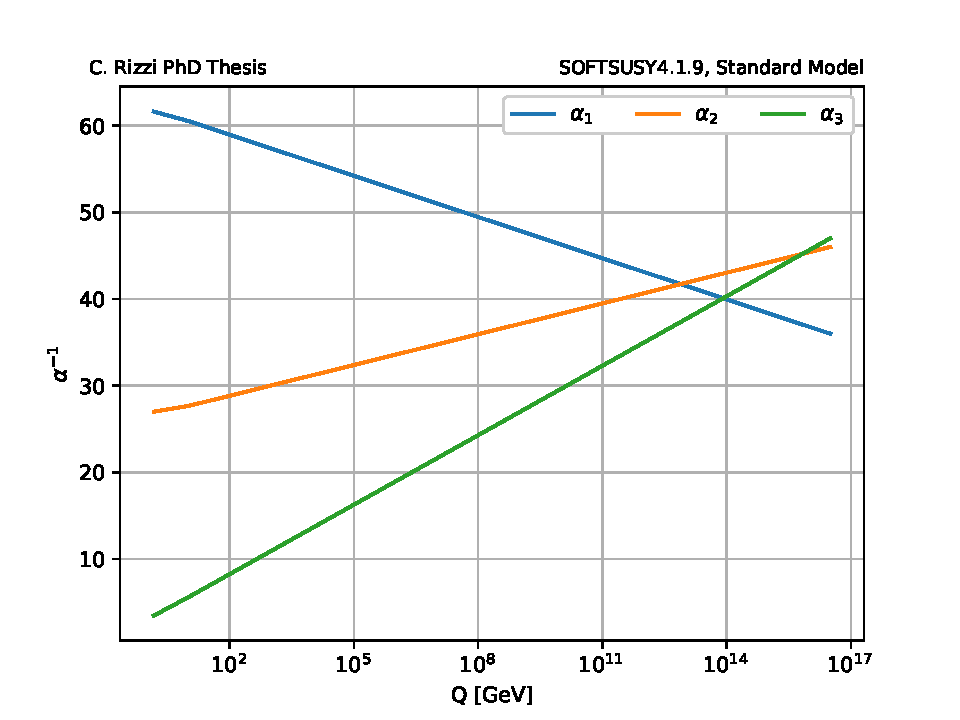
\includegraphics[width=0.45\textwidth]{figures/springer/coupling_constants_SM.pdf}\label{fig:susy:gut_0}}
\subfigure[]{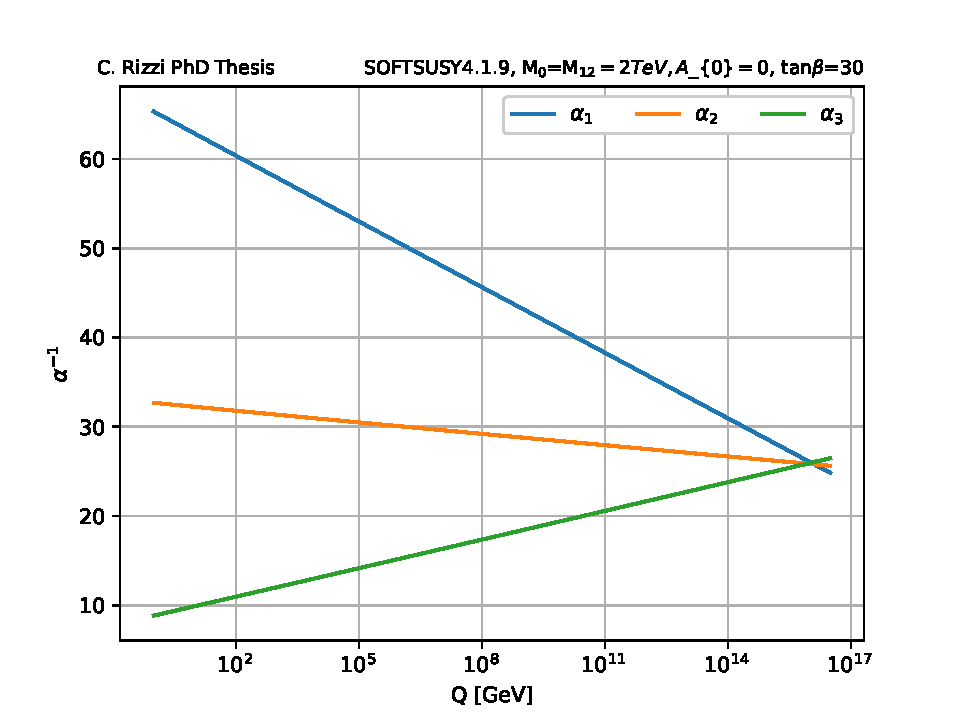
\includegraphics[width=0.45\textwidth]{figures/springer/coupling_constants.pdf}\label{fig:susy:gut_1}}
\caption{Evolution of the gauge couplings with energy scale in \subref{fig:susy:gut_0} the \gls{sm} and \subref{fig:susy:gut_1} the \gls{mssm}. Numbers obtained with SOFTSUSY \cite{Allanach:2001kg}.}
\label{fig:susy:gut}
\end{figure}

\subsubsection*{MSSM Higgs Sector}
\label{sec:susy:Higgs}

To maintain an holomorphic superpotential, \gls{susy} requires at least two SU(2) doublets: one to give mass to up-type quarks ($H_u$) and one to give mass to down-type quarks ($H_d$). The two doublets have eight degrees of freedom. Three of them are  needed to give masses to the gauge bosons, while the other five become observable particles:
\begin{itemize}
\item Two CP-even neutral Higgs bosons: $h^0$ and $H^0$, where $h^0$ is defined to be lighter than $H^0$.
\item $A^0$, a CP-odd Higgs boson.
\item Two charged Higgs bosons, $H^+$ and $H^-$.
\end{itemize}


\subsubsection*{R-parity}

The \gls{mssm} does not include all the possible terms that are gauge- and \gls{susy}-invariant, to avoid interactions that would violate lepton or baryon number conservation. Matter parity, defined as:

\begin{equation}
P_M = (-1)^{3 (B-L)} \; , \nonumber
\label{eq:defmatterparity}
\end{equation}

\noindent is a multiplicative quantum number whose conservation implies automatically the conservation of lepton and baryon numbers (denoted with $L$ and \textit{B} respectively), without having to impose their conservation by hand. Particles in the same supermultiplet have the same matter parity: $P_M =-1$ for lepton and quark supermultiplets, while the Higgs and gauge supermultiplets have $P_M =+1$.

A more convenient way to express the same conservation rule is R-parity:

\begin{equation}
P_R = (-1)^{3(B-L) + 2 s} \; , \nonumber
\label{eq:defRparity}
\end{equation}

\noindent where $s$ is the spin of the particle. This is equivalent to matter parity as $(-1)^{2s}$ is conserved in all interactions where angular momentum conservation holds. The advantage of R-parity over matter parity is that for all \gls{sm} particles $P_R = 1$ and for all \gls{susy} particles $P_R=-1$. If  R-parity is conserved, in a collider experiment \gls{susy} particles are always produced in pairs, and each \gls{susy} particle always has an odd number of \gls{susy} particles in its decay products. As a consequence, the \gls{lsp} is stable; if the \gls{lsp} is electrically neutral, it interacts with ordinary matter mainly through gravity and thus it provides a good candidate for dark matter.

While the consequences of R-parity conservation  are appealing (especially the provision of a dark matter candidate), 
this is just an assumption and is not deduced from the theory.


\subsection{Natural SUSY}
\label{sec:theo:naturalsusy}

Particles within the same supermultiplet share the same electric charge, isospin and \gls{qcd} color, as $Q$ and $Q^\dagger$ commute with the generator of the gauge transformations.
The third equality in Equation \ref{eq:susyalgth} implies that $[ (P^\mu)^2 , Q  ]=0$. If we think of this as an operator applied to a supermultiplet, this implies that all the particles within the same supermultiplet should also have the same mass. The superpartners also bring a radiative correction to the Higgs boson mass, since they couple to the Higgs boson with the same coupling constant as their \gls{sm} partners ($y_S=y_f=y$). If we consider the case of a fermion and a sfermion, according to Eqs. \ref{eq:divhf}--\ref{eq:divhs} the two contributions have opposite sign and the total correction is:

\begin{equation}
\Delta m_H^2 \>=\> {y\over 16 \pi^2}
\left [ m_f^2
\> {\rm ln}(\Lambda_{UV}/m_f) 
- m_S^2
\> {\rm ln}(\Lambda_{UV}/m_S) 
\right] \; . \nonumber
\label{eq:divhsusy}
\end{equation}

This correction cancels if each \gls{sm} particle and its superpartner have the same mass. Unfortunately we know that, if \gls{susy} exists, it must be a broken symmetry, since the superpartners do not have the same mass as the corresponding \gls{sm} particles (otherwise they would have been  
observed already). Since the correction to the Higgs boson mass becomes larger with the increase of the mass difference between particles in the same supermultiplet, \gls{susy} remains a solution to the hierarchy problem as long as this mass difference is reasonably small. The notion of  ``natural \gls{susy}'' refers to the class of \gls{susy} models that allow to solve (or mitigate) the fine-tuning problem that affects the Higgs boson mass; this has been a very active topic of discussion both before the start of the \gls{lhc} (see e.g. Refs. \cite{BARBIERI198863, Dimopoulos:1995mi}) and after (e.g. Refs. \cite{Papucci:2011wy, Casas:2014eca}) 

Not all the superpartners have the same relevance in the contribution to the Higgs-mass corrections, and a \gls{susy} model can be natural even if  most particles in it are extremely heavy. The particles that should be light in a natural \gls{susy} model are:
\begin{itemize}
\item higgsinos, whose tree-level mass is directly controlled by the $\mu$ parameter,
\item stops, which contribute at one loop level to the Higgs boson mass, and
\item gluinos, which contribute at two loops, since they give a one-loop correction to the stop mass.
\end{itemize}


\subsection{SUSY breaking in the MSSM}

Superpartners of the \gls{sm} particles have not been observed yet. This means that, if they exist, their mass must be larger than that of the corresponding \gls{sm} particle, and thus \gls{susy} must be a broken symmetry. The Lagrangian can therefore be written as:

\begin{equation}
\lagr = \lagr_{\rm SUSY} + \lagr_{\rm soft} \; , \nonumber
\end{equation}

\noindent where $\lagr_{\rm SUSY}$ is the \gls{susy}-conserving part derived from the superpotential, while $\lagr_{\rm soft}$ encloses the terms that break \gls{susy}. The suffix ``soft'' means that we allow only soft \gls{susy}-breaking terms in the Lagrangian, whose couplings have positive mass dimension, so that they vanish at very high mass scales. The inclusion of \gls{susy}-breaking terms requires the addition of new particles and interactions to the \gls{mssm}. While there is no unambiguous way to modify the theory to do this (some examples of \gls{susy}-breaking mechanisms are described in Section \ref{sec:susybreaking}), it is possible to include a general parametric form of the \gls{susy}-breaking terms  in the Lagrangian:
\begin{itemize}
\item Gaugino masses, which in the \gls{mssm} correspond to the bino, wino and gluino mass terms;
\item Non-holomorphic scalar squared masses, which add mass terms for squarks and sleptons and contribute to the Higgs potential;
\item Holomorphic scalar squared masses, that in the \gls{mssm} can be present only in a term such as $b H_u H_d$;
\item Scalar cubic couplings.
\end{itemize}  

The necessary \gls{susy}-breaking part of the Lagrangian adds many free parameters to the \gls{mssm}: in total the \gls{mssm} has 105 parameters in addition to the \gls{sm} ones.


\subsection{SUSY-breaking mechanisms}
\label{sec:susybreaking}

The \gls{susy}-breaking terms of $\lagr_{\rm soft}$ can be generated in models where \gls{susy} is spontaneously broken. This is the case if, just like  for the electroweak symmetry breaking, the Lagrangian is \gls{susy}-invariant, but the vacuum state is not. As it happens with the Higgs mechanism, the spontaneous breaking of a symmetry implies the appearance of a massless Goldstone particle (goldstino, $\stilde{G}$) that, in the case of \gls{susy}, has to be a neutral Weyl fermion in order to have the same quantum numbers as the supercharge $Q$. To be massless and annihilate the fermion mass matrix, the goldstino field has to be proportional to:

\begin{equation}
 \stilde{G} \,=\, 
 \begin{pmatrix}
\langle D^a \rangle /\sqrt{2} \cr \langle F_i\rangle 
\end{pmatrix} \; ,
\label{explicitgoldstino}
\end{equation} 

\noindent where $D^a$ and $F_i$ are respectively the auxiliary real bosonic and complex fermion fields of the \gls{susy} Lagrangian, and $\langle \rangle $ denotes their vacuum expectation value. For Equation \ref{explicitgoldstino} to be non-trivial, at least one of the $D^a$ or $F_i$ has to have a non-zero \gls{vev}. This is related to the two possible mechanisms that lead to \gls{susy} breaking: via a $D$-term or an $F$-term. 
The Fayet-Iliopoulos mechanism \cite{Fayet:1974jb} allows a non-zero \gls{vev} for an auxiliary field $D$ by adding to the Lagrangian a term proportional to the auxiliary field itself, with a coupling constant with the dimension of a squared mass:
\begin{equation}
\lagr_{\rm FI} \,=\, -\kappa D \; . \nonumber
\end{equation}
However with this mechanism it is difficult to properly attribute masses to all the \gls{mssm} particles.
%This type of term is gauge-invariant only for abelian groups. 
%the hypercharge symmetry group $U(1)_Y$ is not eligible 

Another possibility is to assign a \gls{vev} to an $F$-term, with the O’Raifeartaigh mechanism \cite{ORaifeartaigh:1975nky}. Since in the \gls{mssm} there is not a good candidate to be a gauge singlet with a non-vanishing \gls{vev} for an $F$-term, this implies the addition of at least one set of chiral supermultiplets, such that $F_i$ is non-trivial for at least one of them. A realization of this is possible for example with three chiral supermupliplets $\Phi_i$ and a superpotential of the form:
\begin{equation}
W = -k \Phi_1 + m \Phi_2 \Phi_3 + {y\over 2} \Phi_1 \Phi_3^2 \;. \nonumber
\end{equation}
The resulting scalar potential at tree level has a minimum for $\phi_2=\phi_3=0$ and is independent of $\phi_1$ (where $\phi_i$ are the scalar fields in $\Phi_i$), while the one-loop corrections lead to a non-zero global minimum when also $\phi_1=0$. In the following we will consider only \gls{susy} breaking originating from the O’Raifeartaigh mechanism.


When \gls{susy} is treated as a local symmetry, it has to include gravity, and the resulting theory is called supergravity. The gravity mediator is the spin-2 graviton, and its superpartner the spin-$\frac{3}{2}$ gravitino. The gravitino can be interpreted as the gauge field of \gls{susy}, and it incorporates the goldstino degrees of freedom upon spontaneous \gls{susy} breaking. Therefore, the gravitino is also indicated with the same symbol as the goldstino, $\stilde{G}$. By dimensional arguments, we can see that the gravitino mass ($m_{3/2}$) has to be proportional to:

\begin{equation}
m_{3/2} \approx \frac{\langle F \rangle}{\Lambda_P} \; ,
\label{mgrav}
\end{equation}
\noindent where $\langle F \rangle$ is the \gls{vev} of the \gls{susy}-breaking $F$-term, as it has to vanish both if \gls{susy} is an exact symmetry and if the Planck scale is extremely high (and thus gravity is negligible). 

For any \gls{susy}-breaking mechanism, the \gls{mssm} soft terms do not appear at tree level, but are generated through radiative corrections. \gls{susy} breaking happens in a hidden sector, while the \gls{mssm} particles live in the visible sector, and experience the consequences of the spontaneous \gls{susy} breaking happening in the hidden sector through interactions that couple both sectors. Depending on which interaction is driving the communication between the \gls{susy}-breaking sector and the \gls{mssm}, we can distinguish three main mechanisms:

\subsubsection*{PMSB} 

If supergravity and the other new physics effects that arise at the Planck scale are responsible for the connection of the hidden sector with the \gls{mssm} sector, then the order of magnitude of the soft parameters in the \gls{mssm} is:
\begin{equation}
m_{\rm{soft}} \approx \frac{\langle F \rangle}{\Lambda_P} \; .
\label{msoft_PMSB}
\end{equation}
\noindent This ratio is motivated by the observation that $m_{soft}$ should vanish both in the limit where \gls{susy} is an exact symmetry, as well as in the limit where the Planck mass is very large and the interactions mediated by gravity are not sizable anymore. We refer to this scenario as \gls{pmsb} \cite{PhysRevLett.49.970, BARBIERI1982343, IBANEZ198273, PhysRevD.27.2359}. In \gls{pmsb} models, the gravitino mass has the same order of magnitude as the mass of the other superpartners (as we can notice by comparing Equation~\ref{mgrav} and Equation~\ref{msoft_PMSB}), and therefore it cannot be particularly light. 

\subsubsection*{AMSB}

If the supergravity couplings that mediate \gls{susy} breaking in \gls{pmsb} models are absent, \gls{susy} can be broken through loop effects. 
In \gls{amsb} models \cite{Randall:1998uk,Giudice:1998xp} scalar and gaugino masses are generated through one-loop corrections arising from superconformal anomalies. These corrections are always present, but are dominant only in models that do not include tree-level terms. 
In the simplest \gls{amsb} model this leads to the prediction of negative squared masses for sfermions; 
one possible extension to the model that solves this problem is the addition of a scalar mass parameter $m_0^2$, 
common to all scalar squared masses. 

\subsubsection*{GMSB}

In the case of \gls{gmsb} \cite{Dine:1981gu, AlvarezGaume:1981wy, Nappi:1982hm, PhysRevD.48.1277, Dine:1994vc, Dine:1995ag} the interactions mediating the connection between the hidden sector and the \gls{mssm} are the same gauge interactions of the \gls{mssm} itself. 
This requires the addition of a set of chiral supermultiplets (mediators) that interact both with the source of supersymmetry breaking and with the \gls{mssm} particles (through loop corrections to their masses, involving the \gls{mssm} gauge interactions). 
The mediators contribute at one loop level to the mass of gauginos, while they have a two-loop contribution to the mass of squarks and leptons. 
In both cases, the mass scale of the superpartners is:
\begin{equation}
m_{\rm{soft}} \approx \frac{\langle F \rangle}{M_\mathrm{mediator}} \; .
\label{msoft_GMSB}
\end{equation}
\gls{sm} gauge bosons are not affected by the loop corrections induced by the mediators, since their mass is protected by the gauge symmetry.
If we compare Equation \ref{msoft_GMSB} with Equation \ref{mgrav} we can see that, as long as the mass of the mediators is lower than the Planck scale, the gravitino can be significantly lighter than the rest of the superpartners. 
In most \gls{gmsb} models the gravitino is the \gls{lsp}. 
While we could expect the decay rate to a $\stilde{G}$ to be low because of the weakness of the gravitational interaction, 
this is not the case as the gravitino inherits the gauge interactions of the goldstino it absorbs during the spontaneous \gls{susy} breaking.  
\gls{susy} breaking introduces a large number of free parameters with respect to the \gls{sm}.
Most of these new parameters lead to flavor-changing interactions that are highly constrained experimentally. 
In models of gauge mediation, the interaction between the \gls{susy}-breaking sector and the \gls{mssm} happens only through gauge interactions, 
which are flavor-blind, and therefore flavor-changing effects are suppressed automatically.


\subsection{Phenomenological MSSM}
\label{sec:theory:pmssm}

The \gls{pmssm} \cite{Djouadi:1998di} reduces the number of free parameters in the \gls{mssm} through some assumptions motivated by experimental evidence. In particular:
\begin{itemize}
\item To avoid flavor changing neutral currents, the sfermion mass matrices and all the trilinear couplings are diagonal. 
\item The presence of CP-violating terms is restricted to only the terms present in the \gls{sm} by imposing that all the new parameters are real numbers.
\item The first two generations of sfermions are degenerate, i.e. the corresponding elements in the first and second generation have the same mass, to circumvent existing limits on the splitting between the first and second squark generations.
\item Since the trilinear couplings give rise to amplitudes that are proportional to the corresponding Yukawa coupling, only the third generation ones are relevant and the others are set to zero.
\end{itemize}

These assumptions allow to reduce the number of free parameters from 105 to 19 (summarized in Table \ref{tab:pMMSpar}), making phenomenological analyses possible.


\begin{table}[h]
\centering
\begin{tabular}{c c}
\hline 
Parameter & Description \\ 
\hline 
\hline
$M_1, M_2  \, M_3 $ & Gaugino mass parameters \\ 
\hline 
$\tan \beta$ & Ratio of the \glspl{vev} of the two Higgs doublets \\ 
\hline 
$M_A$ & Pseudoscalar Higgs boson mass parameter \\ 
\hline 
$\mu$ & Higgsino mass parameter \\ 
\hline 
$  A_t, \, A_b, \, A_\tau    $ & Third generation trlinear couplings \\ 
\hline 
$m_{qL},  \,  m_{uR},  \, m_{dR},  m_{lL},  \, m_{eR}$ & First (and second) generation sfermion masses \\ 
\hline 
 $m_{q3L}, \, m_{tR}, \, m_{bR}, \, m_{\stilde{L}}, \, m_{\stilde{\tau}_R},$ & Third generation sfermion masses \\ 
\hline 
\end{tabular} 
\caption[Free parameters of the \gls{pmssm}]{\label{tab:pMMSpar}List of free parameters in the \gls{pmssm}.}
\end{table}


\clearpage 
\bibliographystyle{atlasBibStyleWithTitle}
\addcontentsline{toc}{section}{Bibliography}
\bibliography{main}


% Supersymmetry (SUSY) is a \gls{bsm} framework that allows to generate an infinite amount of \gls{bsm} models, each with different signatures.

%\glsresetall
\glsunset{atlas}
\glsunset{cms}
\chapter{LHC and ATLAS}
\label{chap:cern}

The analyses presented in this thesis use the \gls{pp} collision data at a center-of-mass energy \cmtre TeV 
collected by the \gls{atlas} experiment in 2015, 2016 and 2017. 

The \gls{atlas} experiment is one of the four main experiments at the \gls{lhc} at the \gls{cern}. Section \ref{sed:cern:lhc} of this chapter describes the \gls{lhc} accelerator complex. This is followed by a general description of the detectors used in high-energy physics in Section \ref{sec:detectors}. The \gls{atlas} detector is discussed in Section \ref{sed:cern:atlas}.

%%%%%%%%%%%%%%%%%% LHC

\section{The Large Hadron Collider}
\label{sed:cern:lhc}

In this section we give a brief introduction to the \gls{lhc} \cite{1748-0221-3-08-S08001}, at the moment the largest and most powerful particle accelerator in the world, hosted by \gls{cern} and in operation since September 2008.
The first data for physics have been collected in the period  between 2010 and 2013, referred to as Run 1, at the center-of-mass energy of \cmsette and later 
\cmotto TeV, delivering to \gls{atlas} 5.5 \ifb at \cmsette TeV and 22.8 \ifb at \cmotto TeV.
After a shutdown of two years, in 2015 the \gls{lhc} started the Run 2 data taking at \cmtre TeV, which will continue until the end of 2018. 
In 2015--2017 the \gls{lhc} has delivered to \gls{atlas} 93 \ifb of \gls{pp} collisions. 

\subsection{A circular hadron collider}

The \gls{lhc} is a circular hadron accelerator, located in a 26.7 km long underground tunnel (with a depth ranging between 50 and 140 meters) that was previously hosting the \gls{lep}, a \gls{cern} accelerator that was operational from 1989 to 2000. The \gls{lhc} can accelerate protons up to a design center-of-mass energy of 13 TeV. Accelerating particles to very high energies is necessary both to study the structure of the particles themselves at smaller scales, and to create heavy states in collisions. Cosmic rays provide a source of particles with energies up to $10^7$ times higher than what the \gls{lhc} is capable of, but these extremely energetic rays are very rare, and is is not possible to modify the flux. 
Accelerators provide a well controlled flux of particles of a specific type in a specific location, and this allows the study of these particles with dedicated detectors.

A circular accelerator simplifies the acceleration of particles, as this can happen over several revolutions. When a charged particle travels on an orbit of radius $r$ under the effect of a magnetic field \textit{B}, its momentum $p$ is given by:
\begin{equation}
\label{eq:cern:p03br}
p = 0.3 r B,
\end{equation}
\noindent where the momentum is expressed in GeV, \textit{B} in Tesla and the radius of the orbit in meters. For a given magnetic field, a larger radius allows to reach higher energies. 

The choice of a collider over a fixed-target experiment is motivated by the possibility of reaching a higher energy in center-of-mass of the system: while in a fixed-target experiment this is proportional to the square root of the energy of the incoming particle, in a collider it is the sum of the energies of the two beams.


Suitable particles for a collider experiment need to fulfill two criteria: they need to be charged, in order to be accelerated and guided through electric and magnetic fields, and they need to be stable enough not to decay before being used for collisions. These criteria effectively limit the choice to protons, electrons, their antiparticles and ions. 

At the \gls{lhc} it has been chosen to study collisions with protons and lead ions. Three types of collisions are studied: \gls{pp}, lead-lead ($Pb$-$Pb$) and also proton-lead ($Pb$-$p$). The main reason to prefer protons over electrons is the energy loss that affects charged particles accelerated in a circular trajectory (syncrotron radiation), which decreases with the fourth power of the mass of the particle:

\begin{equation}
\label{eq:cern:sync}
\frac{dE}{dt} \propto \frac{E^4}{m^4 r^2} \; . \nonumber
\end{equation}

The larger mass of a proton with respect to an electron leads to a decrease by a factor $10^{12}$ in the energy lost through syncrotron radiation. This choice comes with a price: proton-proton collisions lead to less clean events, with a lot of soft interactions covering the interesting hard interactions. Furthermore, the center-of-mass energy is unknown as the particles taking part in hard interactions are not the protons themselves but their constituents.

\subsection{Magnet system} 


The \gls{lhc} is not a perfect circumference: it is composed of eight arcs (sectors), where the magnetic system is located, and eight straight sections containing the resonant cavities, the four interaction points with and the detectors, the equipment for beam injection and extraction, and other instrumentation. Magnetic fields are used to govern the trajectory of particles. In the \gls{lhc} there are more than nine thousand magnets, constructed from a superconducting alloy of niobium and titanium. About 150 tons of super-fluid helium at a temperature of 1.9 K are used to maintain the magnet system in the superconducting regime. Different types of magnets are necessary to achieve a proper control over the trajectory of particles.

\subsubsection*{Dipoles} 
Dipoles are used to create a vertical magnetic field, so as to bend the particles in the horizontal plane and thus give the dominant circular orbit. The \gls{lhc} has 1232 dipoles, each 15 m long and providing a magnetic field of 8.3 T. The current necessary to achieve this strong magnetic field is 11.8 kA.


\subsubsection*{Quadrupoles}
The \gls{lhc} has 858 quadrupoles, used for beam focusing. A single quadrupole can focus the beam either in the vertical or the horizontal plane, but it causes a defocusing in the other plane; conventionally a quadrupole is denoted as focusing if it is oriented to focus in the horizontal plane. A combination of focusing and defocusing quadrupoles separated by some drift space (FODO lattice) is used to keep both planes focused, and gives rise to Betatron oscillations. 

\subsubsection*{Higher-order magnets} 
Beside dipoles and quadrupoles, in the \gls{lhc} there are about 600 higher-order magnets that are used to maintain a good beam quality; e.g.  sextupoles are used to correct the spread in Betatron tune caused by the quadrupoles.



\subsection{Resonant cavities}

While the orbit of particles is governed by the magnetic fields, longitudinal electric fields are used for acceleration. In the \gls{lhc} the electric filed is provided by \gls{rf} cavities. There are overall 16 \gls{rf} cavities, eight per beam, hosted in four cryo-modules. Each cavity can provide an accelerating field of 5 MV/m, and oscillates with a frequency of 400 MHz. Since the electric field changes over time with the oscillations, particles passing through the same point of a \gls{rf} cavity at different times experience a different voltage; this produces a non-trivial longitudinal dynamics, where particles oscillate around the ideal synchronous particle with changes in momentum and phase (synchrotron oscillations). If we define the slip factor $\eta$ as the relative change in frequency in synchrotron oscillations with the relative change in momentum:
\begin{equation}
\eta = \frac{\Delta f / f}{\Delta p / p} \; , \nonumber
\end{equation}

\noindent and the compaction factor $\alpha$ as the relative change in frequency in orbit length with the relative change in momentum:

\begin{equation}
\alpha = \frac{\Delta L / L}{\Delta p / p} \; , \nonumber
\end{equation}

\noindent the following relation holds:

\begin{equation}
\eta = \frac{1}{\gamma^2} - \alpha \; , \nonumber
\end{equation}

\noindent where $\gamma$ is the Lorentz factor of the particle. This means that while the energy of the particle is low ($\eta>0$) an increase in momentum leads to an increase in frequency, while it leads to a decrease in frequency for $\eta<0$. At the transition energy, a previously stable synchrotron phase becomes unstable and vice versa; this requires a rapid change in \gls{rf} phase. This situation is illustrated in Figure \ref{fig:lhc:phase}(a). For example, a particle corresponding to the phase point A1 will arrive in the \gls{rf} cavity after one corresponding to the stability point P1, and will experiment higher voltage and increase in momentum; if $\eta>0$ this increase in momentum will translate in an increase in frequency and the particle will, at the following revolution, arrive earlier, while if $\eta<0$ the frequency will further decrease and the particle will be eventually lost.  The transition energy in the \gls{lhc} is 53 GeV, well below the injection energy of 450 GeV, so the \gls{lhc} is always above transition. 

\begin{figure}[ht]
\centering
\subfigure{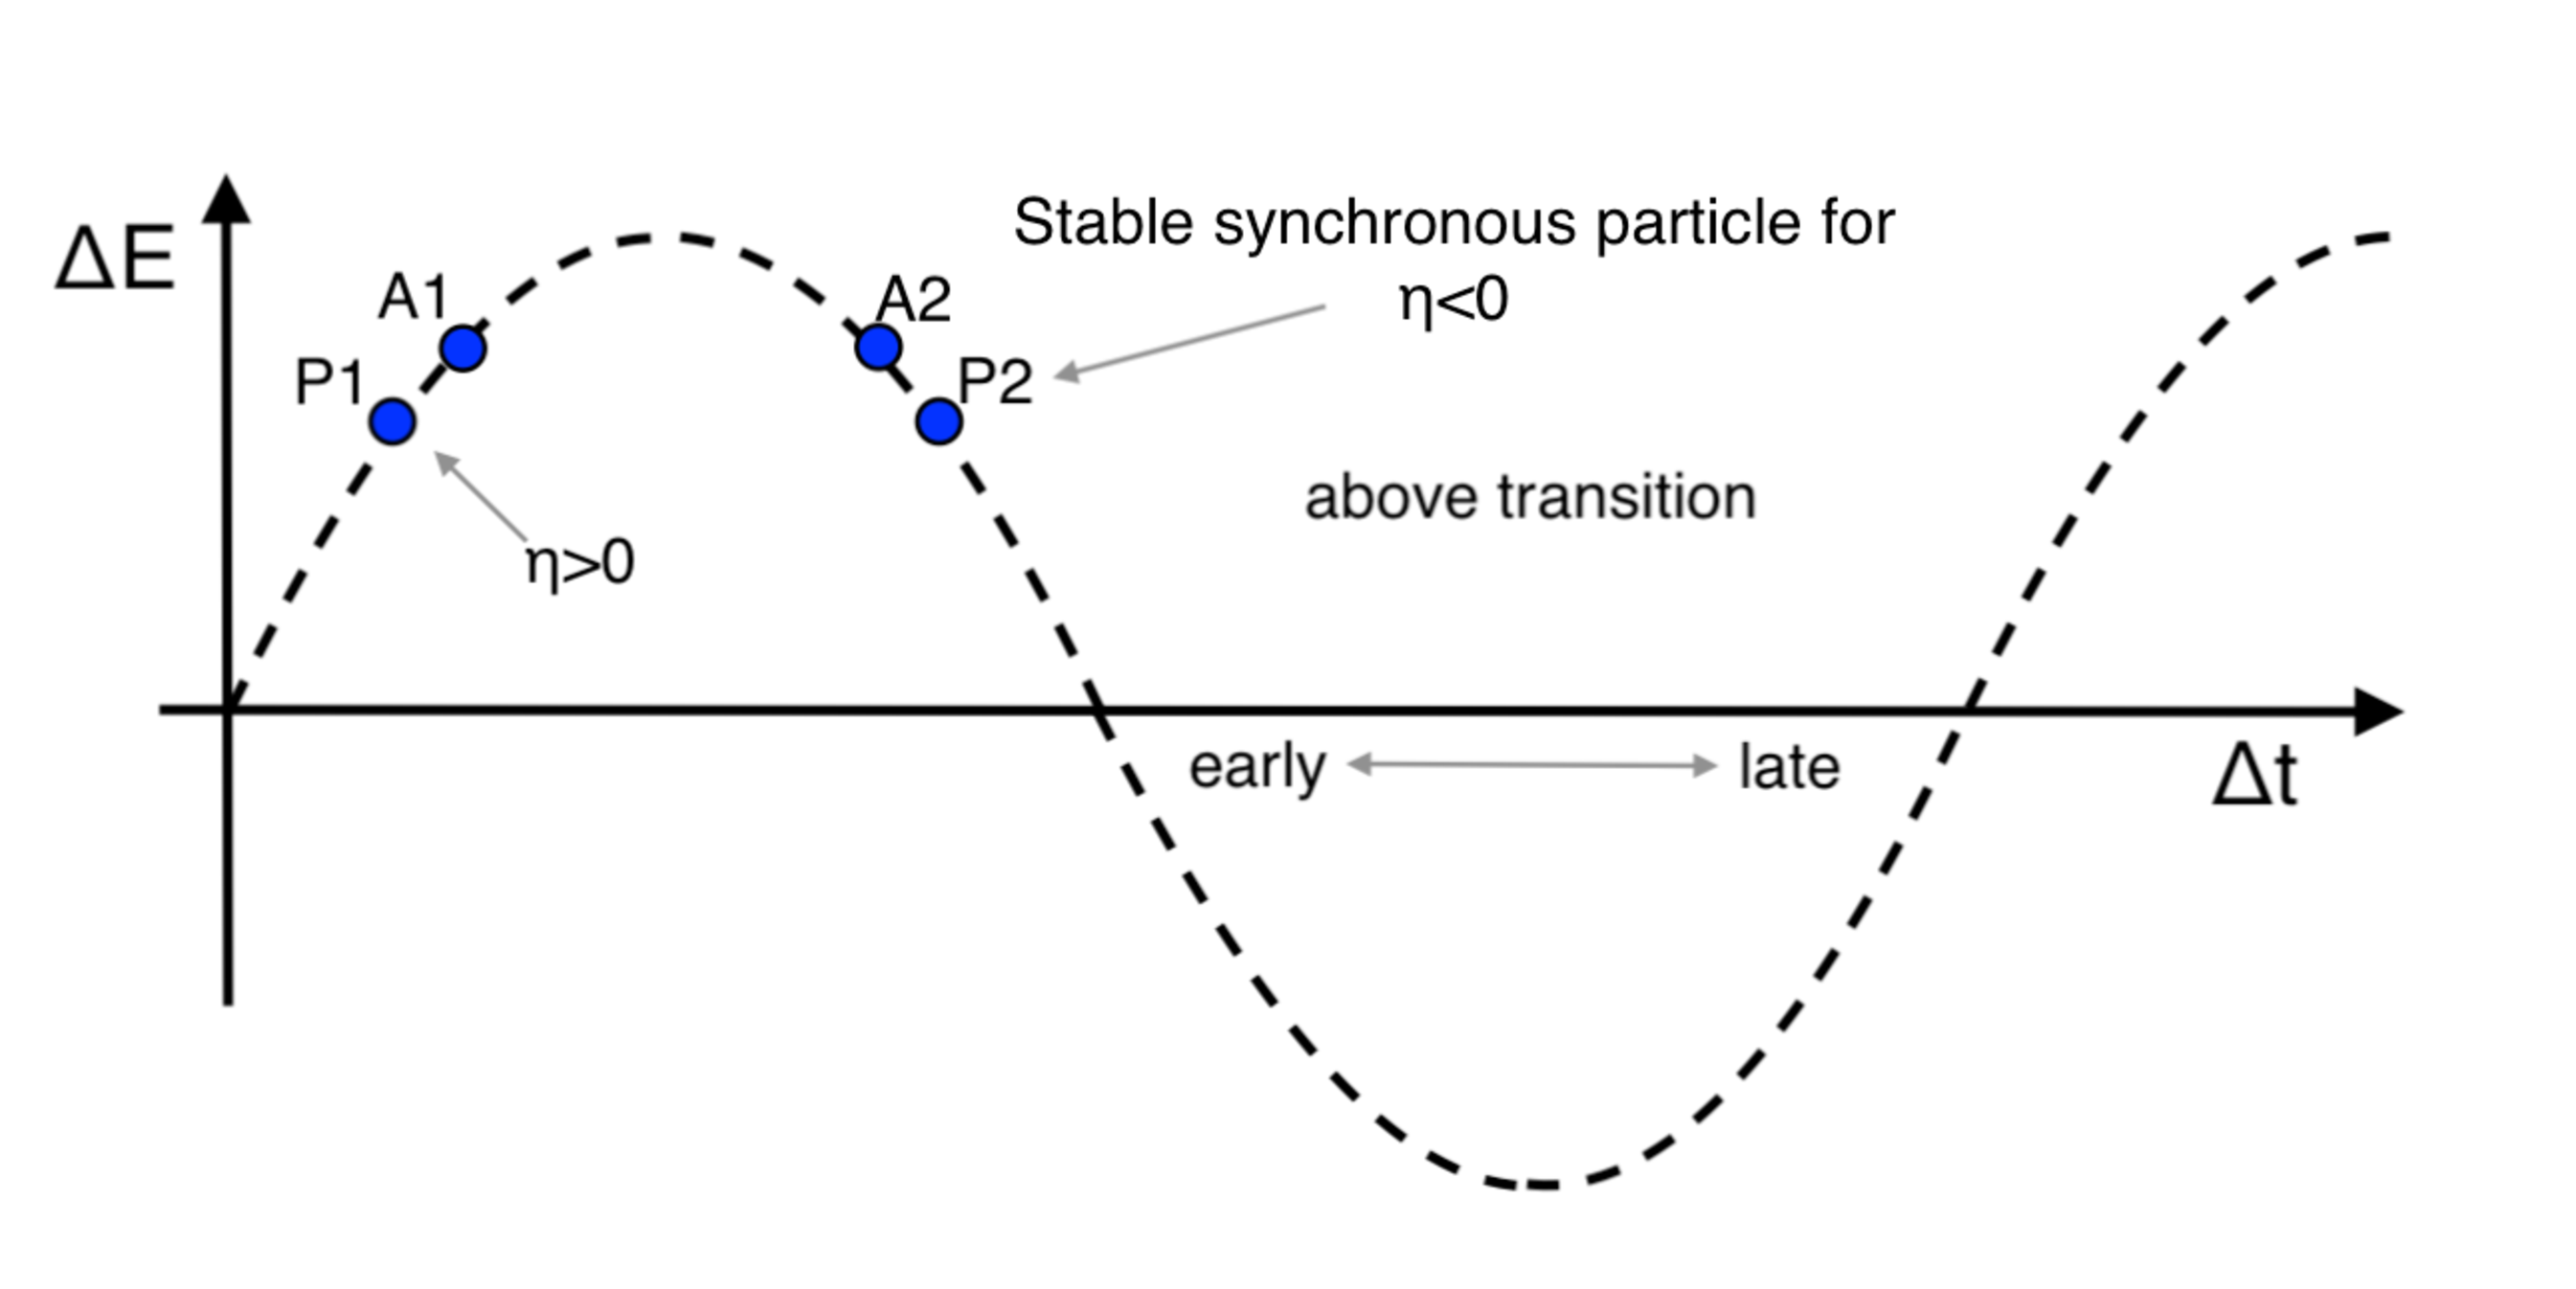
\includegraphics[width=0.547\textwidth]{figures/Chap3/Rizzi-Fig3-1-1.pdf}}
\subfigure{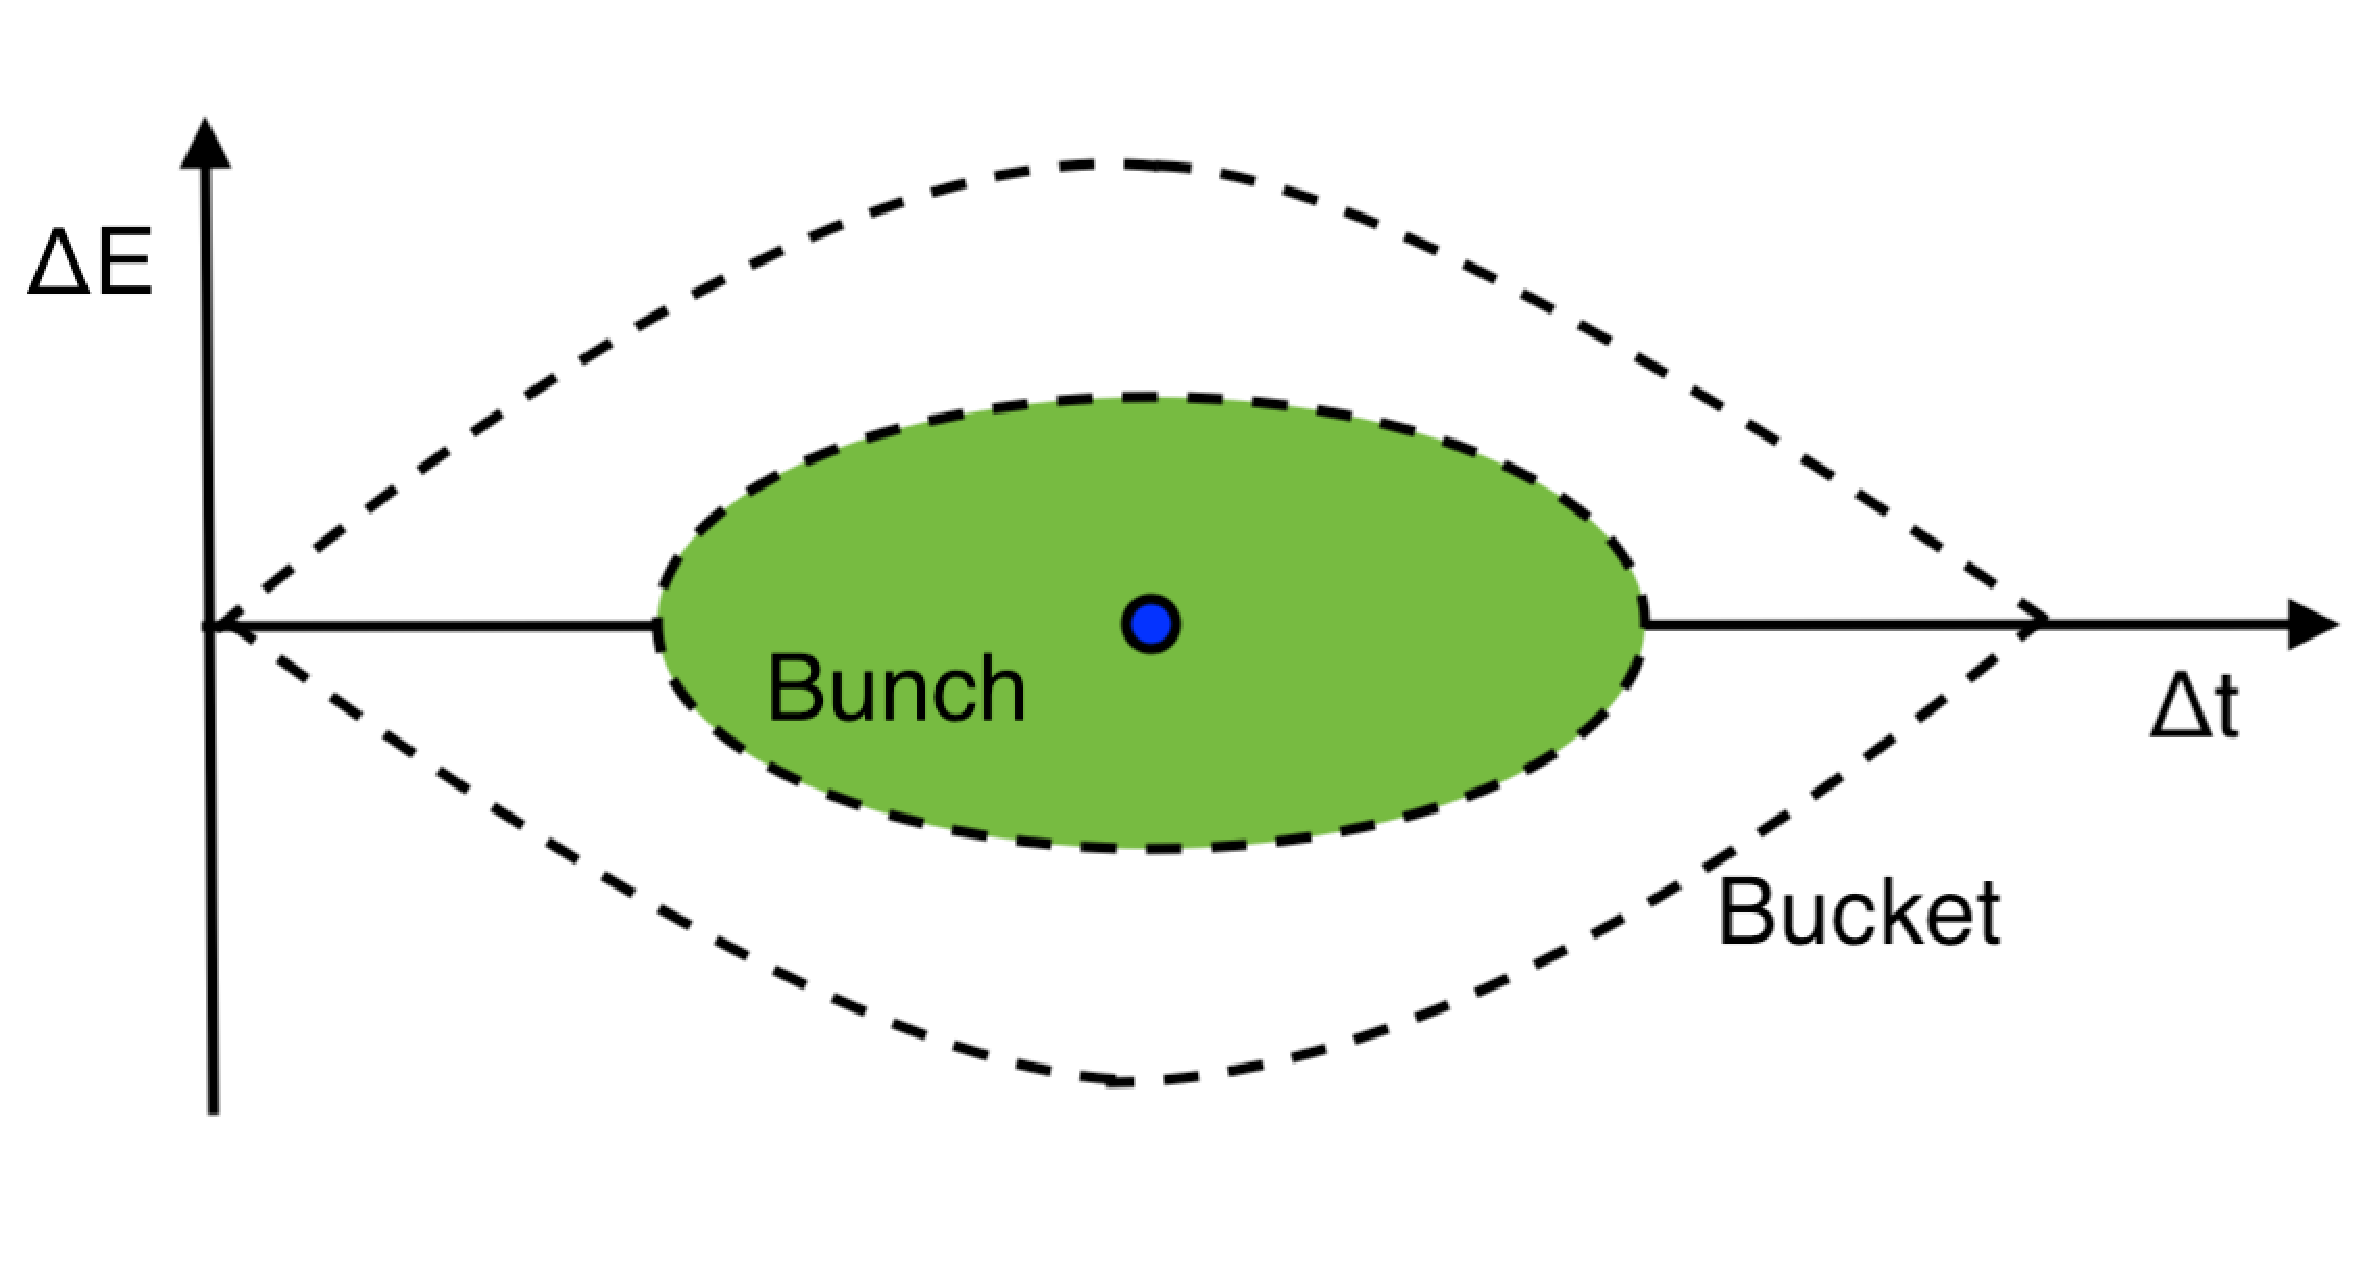
\includegraphics[width=0.44\textwidth]{figures/Chap3/Rizzi-Fig3-1-2.pdf}}
\caption{(a) Phase stability below and above transition. (b) Bucket and the bunch for a beam above the transition energy. 
Figures based on the discussion in Ref. \cite{Tecker:2016mlq}.}
\label{fig:lhc:phase}
\end{figure}


In the \gls{lhc} beams particles are not distributed continuously, as this would not be allowed by phase instabilities, but are divided in bunches. 
The areas of stable motion are identified as bucket, and the area of the bucket is the beam longitudinal acceptance. 
The beam bunches fill only a part of the bucket, and the area of the beam bunches is the longitudinal beam emittance. Figure \ref{fig:lhc:phase}(b) shows a schematic view of the bucket and the bunch area for the case of a beam above the transition energy. 

\subsection{Luminosity and operational parameters}

The amount of data delivered by an accelerator is quantified by the integrated luminosity $\mathcal{L}_{int}$.
Given a certain process with production cross-section $\sigma$, the total number of events for that process is the product of cross-section and integrated luminosity:

\begin{equation}
\label{eq:cern:nev}
N_{\mathrm{events}} = \sigma \,\, \mathcal{L}_{int} \; . \nonumber
\end{equation}

The integrated luminosity is the time integral of the instantaneous luminosity $\mathcal{L}$, 

\begin{equation}
\label{eq:cern:intlumi}
\mathcal{L}_{int} = \int \mathcal{L} \, dt \; , \nonumber
\end{equation}

\noindent which, assuming a Gaussian particle distribution and the same characteristics for the two beams, can be expressed as:

\begin{equation}
\mathcal{L}=\frac{f N_b n^2}{4 \pi \sigma_{x}\sigma_{y} } \; , 
\label{eq:cern:lumi}
\end{equation}

\noindent where $f$ is the revolution frequency, $N_b$ the number of bunches in each beam, $n$ the number of protons in each bunch and $\sigma_{x(y)}$  is the transverse beam size at the interaction point in the $x$($y$) direction . 

The instantaneous luminosity defined in Equation \ref{eq:cern:lumi} needs to be corrected for two effects. First of all, this formula assumes a head-on collision between the bunches; in reality, to avoid unwanted interactions the beams collide with a crossing angle, and a large crossing angle decreases the instantaneous luminosity. The second correction is related to the beam transverse size, that can be expressed as:
\begin{equation}
\sigma_{x,y} = \sqrt{  \epsilon \beta^* } \; , \nonumber
\end{equation}
where $\epsilon$ is the beam emittance and $\beta^*$ is the beta function. Beam collisions happen in minibeta insertions, drift spaces with a beta waist in the center, where the beam size is as small as possible. In the vicinity of the minimum, the beta function evolves like:

\begin{equation}
\beta(s) = \beta^* + \frac{s^2}{\beta^*} \; . \nonumber
\end{equation}

From this it is possible to see that the smaller the beta function, the larger the dependence with $s$, so a bunch with a finite size will not have the same beta function as a whole (hour glass effect). This correction becomes more important with the decrease of the $\beta^*$ value. With the \gls{lhc} design parameters, the effect of crossing angle and hour glass changes the instantaneous luminosity by about 20\%.

The main limitations in the choice of the parameters that regulate the luminosity are collective effects, which could cause beam instabilities if the number of bunches or the number of protons per bunch is too high, and the limitations in the available aperture in the
quadrupoles focusing the beam in the minibeta insertions, that impacts $\beta^*$. The summary of the \gls{lhc} operational parameters during Run 2 is reported in Table \ref{tab:lhc:param}.


\begin{table}[ht]
\begin{center}
\begin{tabular}{c c c c c }
\hline 
Parameter & 2015 & 2016 & 2017 & Design \\ 
\hline 
\hline
Protons per bunch (n) [$10^{11}$ p] & $\approx$ 1.2 & $\approx$ 1.1 & $\approx$ 1.2 & 1.15 \\ 
\hline 
Number of bunches (N$_b$) & 2244 & 2220 & $\approx$ 2250 & 2780 \\ 
\hline 
Emittance ($\epsilon$) [mm mrad] & $\approx$ 3.5 & $\approx$ 2.2 & $\approx$ 2.2 & 3.5 \\ 
\hline 
Beta function ($\beta^*$) [cm] & 80 & 40 & 40 (30) & 55 \\
\hline
Crossing angle [$\mu$rad] & 290 & 370 (280) & 300 (340) & 285 \\
\hline
Peak luminosity [$10^{34}$ cm$^{-2}$s$^{-1}$] & 0.51 & 1.4 & 1.7(1.9) & 1.0 \\
\hline
\end{tabular}
\end{center}
\caption{\gls{lhc} operational parameters in Run 2 compared to their design value.
The numbers in parenthesis report changes in the parameters during the year. 
E.g. in 2016 the crossing angle was reduced after fill 5300,
while for 2017 the numbers in parenthesis report the values 
after the recommissioning with $\beta^* = 0.3$ m.}
\label{tab:lhc:param}
\end{table}


The luminosity profile changes over time, and different experiments have different luminosity needs. \gls{atlas} and CMS profit from having the maximum luminosity possible, while LHCb and ALICE have their top functionality at lower luminosity, and therefore apply a luminosity leveling that consists in changing the offset of the beams during the run, to maintain a constant (low) value of the instantaneous luminosity.

A high number of particles participating in a single bunch crossing can lead to a large number of multiple proton-proton collisions (pileup). In 2012 the \gls{lhc} operated with a bunch spacing of 50 ns, leading to a pileup of about 35 events per bunch crossing. With the increase in energy from Run 1 to Run 2, the same settings would have implied more than 100 events, above the limit for the proper functioning of the detectors. This is what motivated the choice to move from the 50 ns bunch spacing used in Run 1 to the 25 ns in Run 2: with this setup, for the same instantaneous luminosity is possible to have a lower ``per-bunch luminosity'' and therefore a lower pile up. Figure \ref{fig:atlas:pu} shows the luminosity-weighted distribution of the mean number of interactions per crossing during Run 1 (in Figure \ref{fig:atlas:pu:run1})
and in 2015--2017 (in Figure \ref{fig:atlas:pu:run2}) as recorded by the \gls{atlas} experiment.

\begin{figure}[ht]
\centering
\subfigure{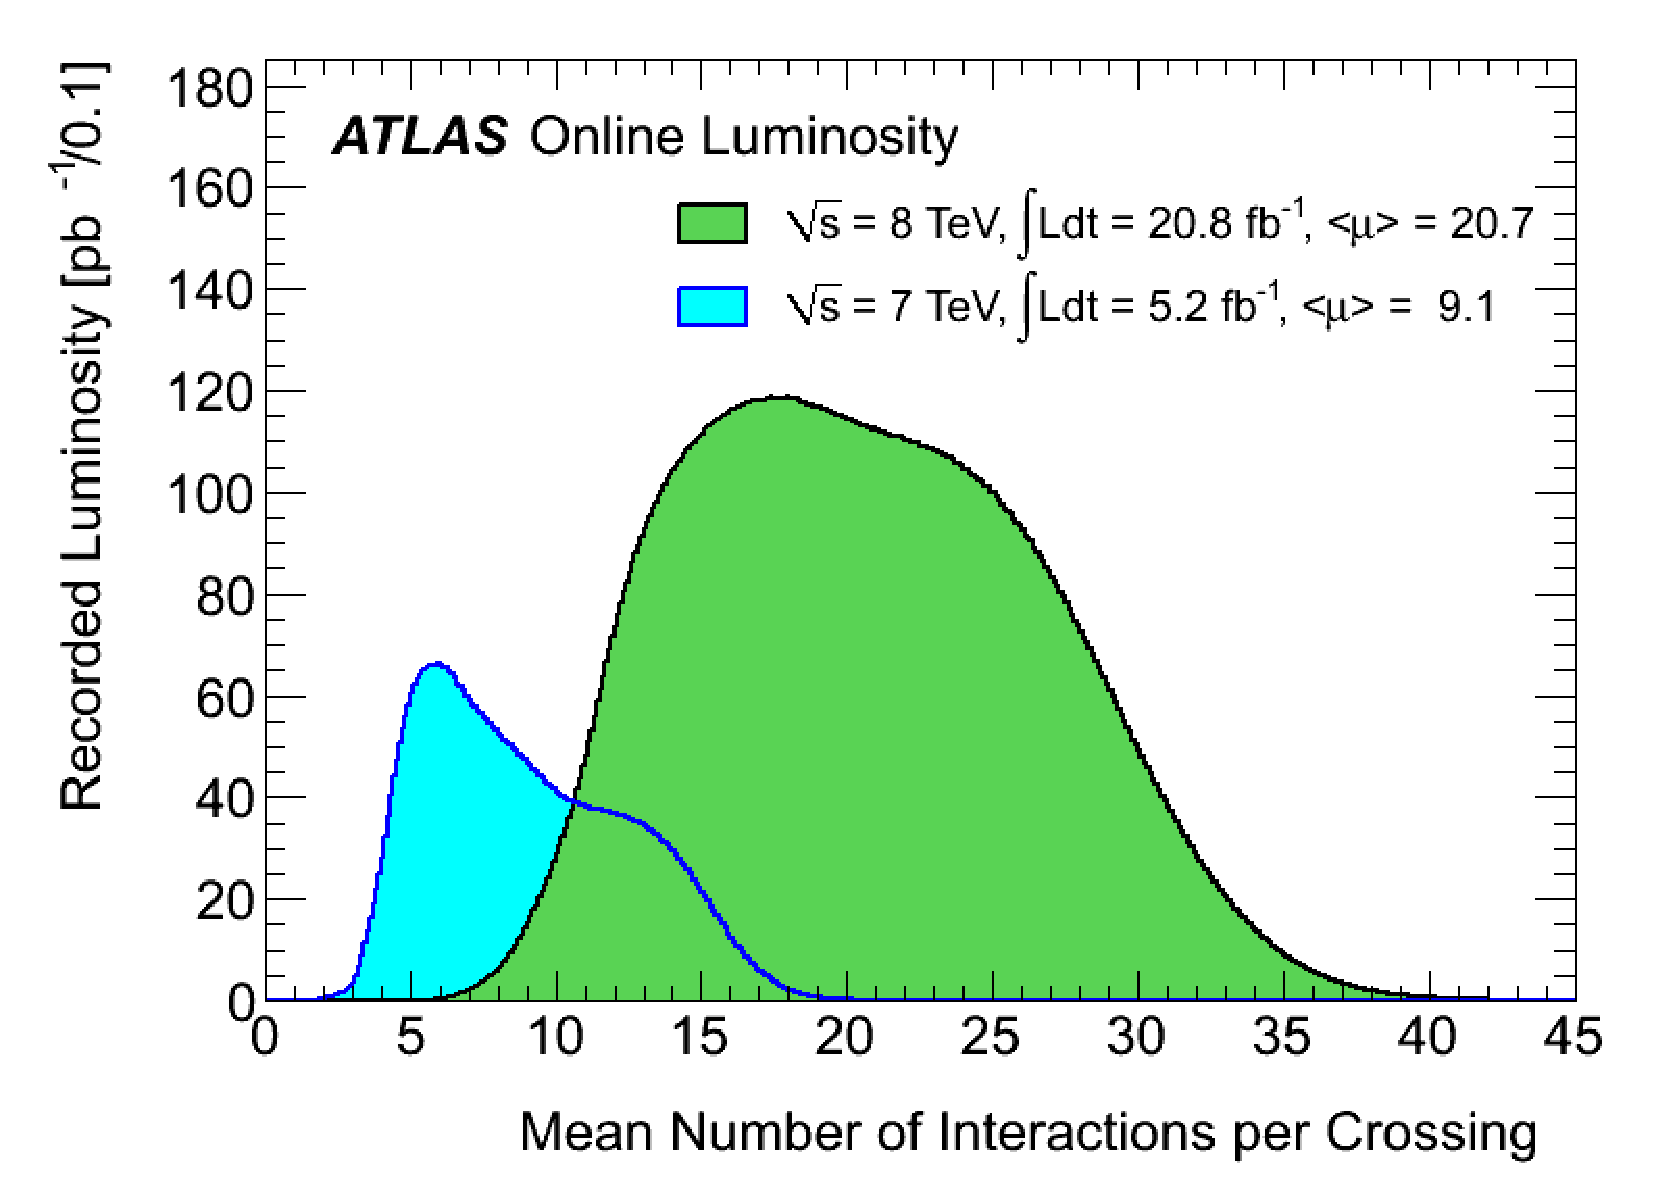
\includegraphics[width=0.49\textwidth]{figures/Chap3/Rizzi-Fig3-2-1.pdf}\label{fig:atlas:pu:run1}}
\subfigure{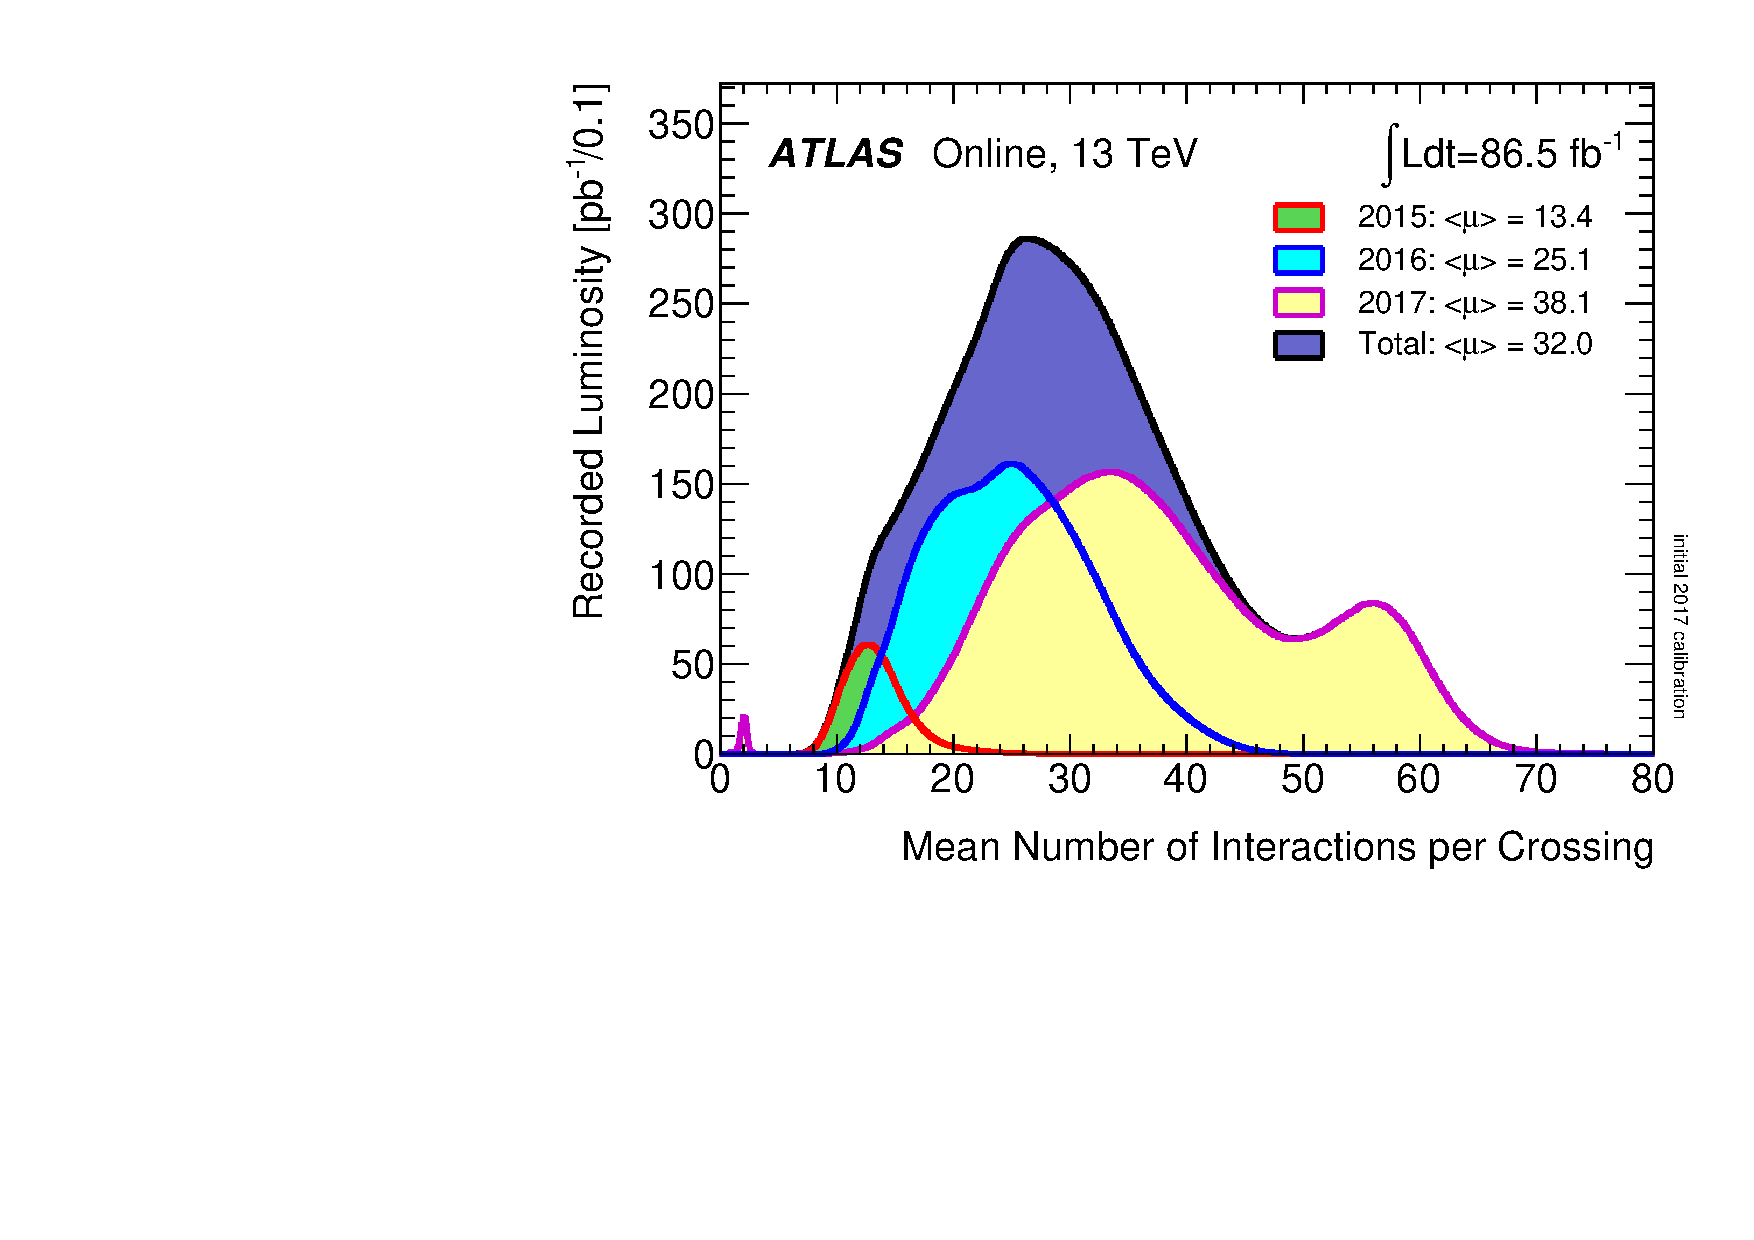
\includegraphics[width=0.49\textwidth]{figures/Chap3/Rizzi-Fig3-2-2.pdf}\label{fig:atlas:pu:run2}}
\caption{Luminosity-weighted distribution of the mean number of interactions per crossing in 
\subref{fig:atlas:pu:run1} Run 1 and \subref{fig:atlas:pu:run2} Run 2 (2015--2017). All data recorded by \gls{atlas} during stable beams is shown. The mean number of interactions per crossing $\mu$ corresponds to the mean of the Poisson distribution of the number of interactions per crossing calculated for each bunch. It is calculated from the instantaneous per-bunch luminosity as 
$\mu = \mathcal{L}_{bunch}\sigma_{inel}/f$, where $\mathcal{L}_{bunch}$ is the per-bunch instantaneous luminosity, $\sigma_{inel}$ is the inelastic cross-section which is taken to be 80 mb for 13 TeV collisions, and $f$ is the \gls{lhc} revolution frequency. Figures from Ref. \cite{LumiTwiki}.}
\label{fig:atlas:pu}
\end{figure}


\subsection{Accelerator complex}

Protons are injected in the \gls{lhc} only after being accelerated to 450 GeV by a sequence of machines.

\begin{itemize}
\item Protons are extracted from $H_2$ at the Linac2 facility, a linear accelerator of 33 m that brings them to the energy of 50 MeV.
\item The \gls{psb} is the first synchrotron in the acceleration chain (with a circumference of 157 m), that in 1.2 s increases the energy of the protons from 50 MeV to 1.4 GeV.
\item With a circumference of 628 m, the \gls{ps} brings the protons to about 26 GeV. This was the oldest synchrotron experiment at \gls{cern}.
\item The \gls{sps} is the first accelerator of the chain to be underground (about 30 m) and has a circumference of 6.9 km; it brings the proton energy at 450 GeV. Beside preparing the protons to be injected into the \gls{lhc}, the \gls{sps} provides beam also to the North Area, 
where the beams for fixed-target experiments are prepared, 
and to the AWAKE experiment, that studies proton-induced plasma wakefield acceleration.
\item The \gls{lhc} is the last step of this chain, and it accelerates the protons form 450 GeV to 6.5 TeV (the design energy is 7 TeV); 
in the \gls{lhc} the protons gain about 0.5 MeV per turn, so it takes about 15 minutes to reach 6.5 TeV.
\end{itemize}

The accelerator complex of \gls{cern} is shown in Figure \ref{fig:lhc:acc}. The acceleration chain for lead ions differs from the one for protons in the initial part, which consists in Linac3  and \gls{leir} before the injection in the \gls{ps}. 

\begin{figure}[ht]
\centering
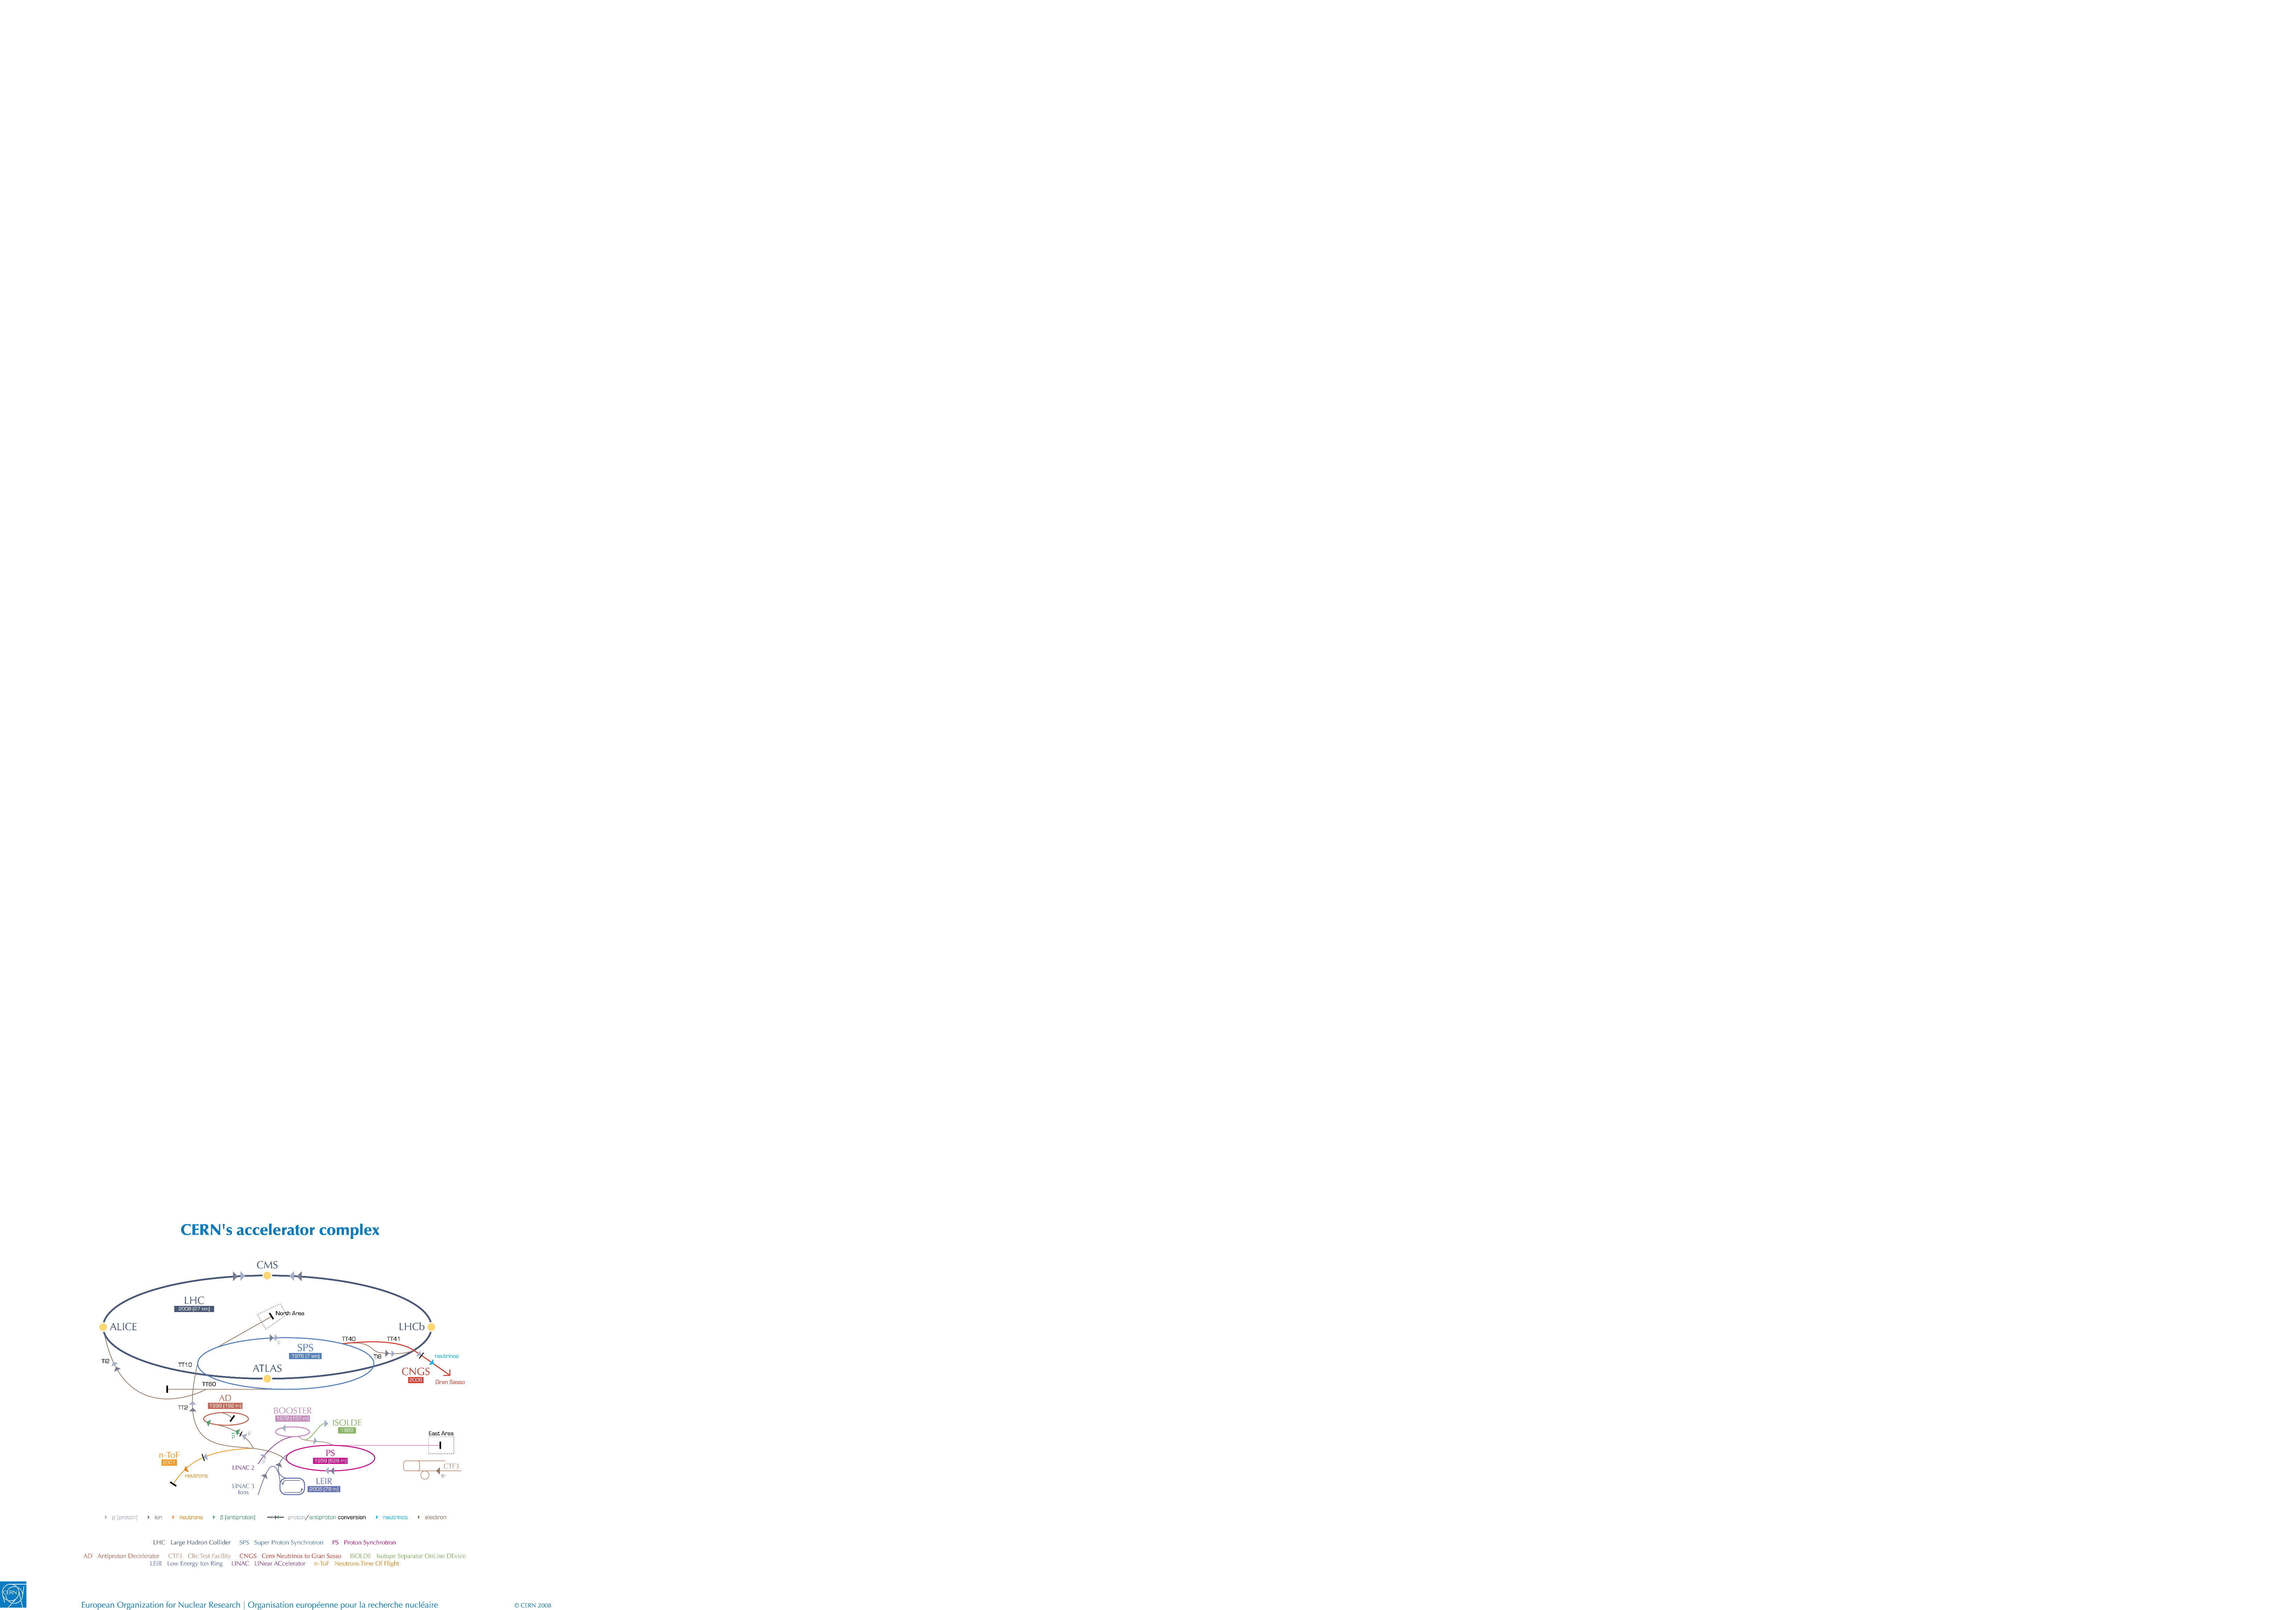
\includegraphics[width=1\textwidth]{figures/Chap3/Rizzi-Fig3-3.pdf}
\caption{ Schematic view of the \gls{cern} accelerator complex. The four main \gls{lhc} experiments are shown at the interaction points. Figure from Ref. \cite{Christiane:1260465}.}
\label{fig:lhc:acc}
\end{figure}

\subsection{Experiments at the LHC}

Seven experiments are built along the \gls{lhc} circumference and collect the data produced during the collisions. Each experiment is run by an independent collaboration that comprises several universities and research institutes. 
\gls{atlas} \cite{atlas:atlas} and CMS \cite{cms:cms} are the two largest and general purpose experiments, located at two opposite sides of the \gls{lhc} ring, in correspondence with two of the four interaction points. Their goal is to study a large variety of SM processes and to perform an extensive search program for \gls{bsm} physics. The independent design of the two detectors, as well as of the separation between the two collaborations running them, is essential to provide a validation of the \gls{lhc} results. Since the data used in this thesis is collected with the \gls{atlas} detector, a more extensive description of this experiment is given in Section \ref{sed:cern:atlas}. 
The LHCb \cite{lhcb:lhcb} and ALICE \cite{alice:alice} experiments are located at the other two \gls{lhc} interaction points. LHCb is a single-arm forward spectrometer, designed to perform high-precision studies of heavy flavor physics. The ALICE experiment is dedicated to the study of $Pb-Pb$ collisions, which at the \gls{lhc} happen with a center-of-mass energy of 2.6 TeV per nucleon pair; in this energy regime, quarks and gluons are expected to form a quark-gluon plasma.
The position of the four main experiments on the \gls{lhc} ring is shown in Figure \ref{fig:lhc:acc}.
Other three smaller experiments are installed along the \gls{lhc} circumference: TOTEM \cite{totem:totem}, LHCf \cite{lhcf:lhcf} and MoEDAL \cite{moedal:moedal}. TOTEM is located at the same interaction point as CMS, and measures the total \gls{pp} cross-section, as well as elastic and inelastic scattering. LHCf is installed in the same interaction point as \gls{atlas} and has two detectors, at 140 m from each side of the collision point, aiming at the study of particles produced in the ``forward'' region (very close to the beam axis). MoEDAL is installed in the LHCb cavern and is designed to search for magnetic monopoles.  


%%%%%%%%%%%%%%%%%% 

\section{Detectors for collider Physics}
\label{sec:detectors}

In this section we review the basic concepts that drive the design of the \gls{lhc} detectors, including \gls{atlas}.

\subsection{Identification of particles}
\label{sec:detectors:identification}



The ability to accurately identify particles and reconstruct their energy and trajectory is what drives the design of detectors for high energy physics. In a detector, different sub-systems are able to capture different types of particle interactions, and the combination of the information collected by each of them allows to identify particles (or at least assign them to families, such as neutral or charged hadrons). A typical schema of the subdetectors sequence is shown in Figure \ref{fig:detector:interaction}. The innermost layer, closer to the interaction point, is the tracking system, dedicated to the measurement of the signed charge and momentum of charged particles. The following layers are the electromagnetic and hadronic calorimeters, that measure the energy of particles with electromagnetic and hadronic interactions respectively. The outermost layer is dedicated to the muon system: because of their large mass (about 200 times more than electrons) muons do not produce electromagnetic showers and are therefore easy to identify as they are the only detectable particles that reach the external part of the detector.

\begin{figure}[ht]
\centering
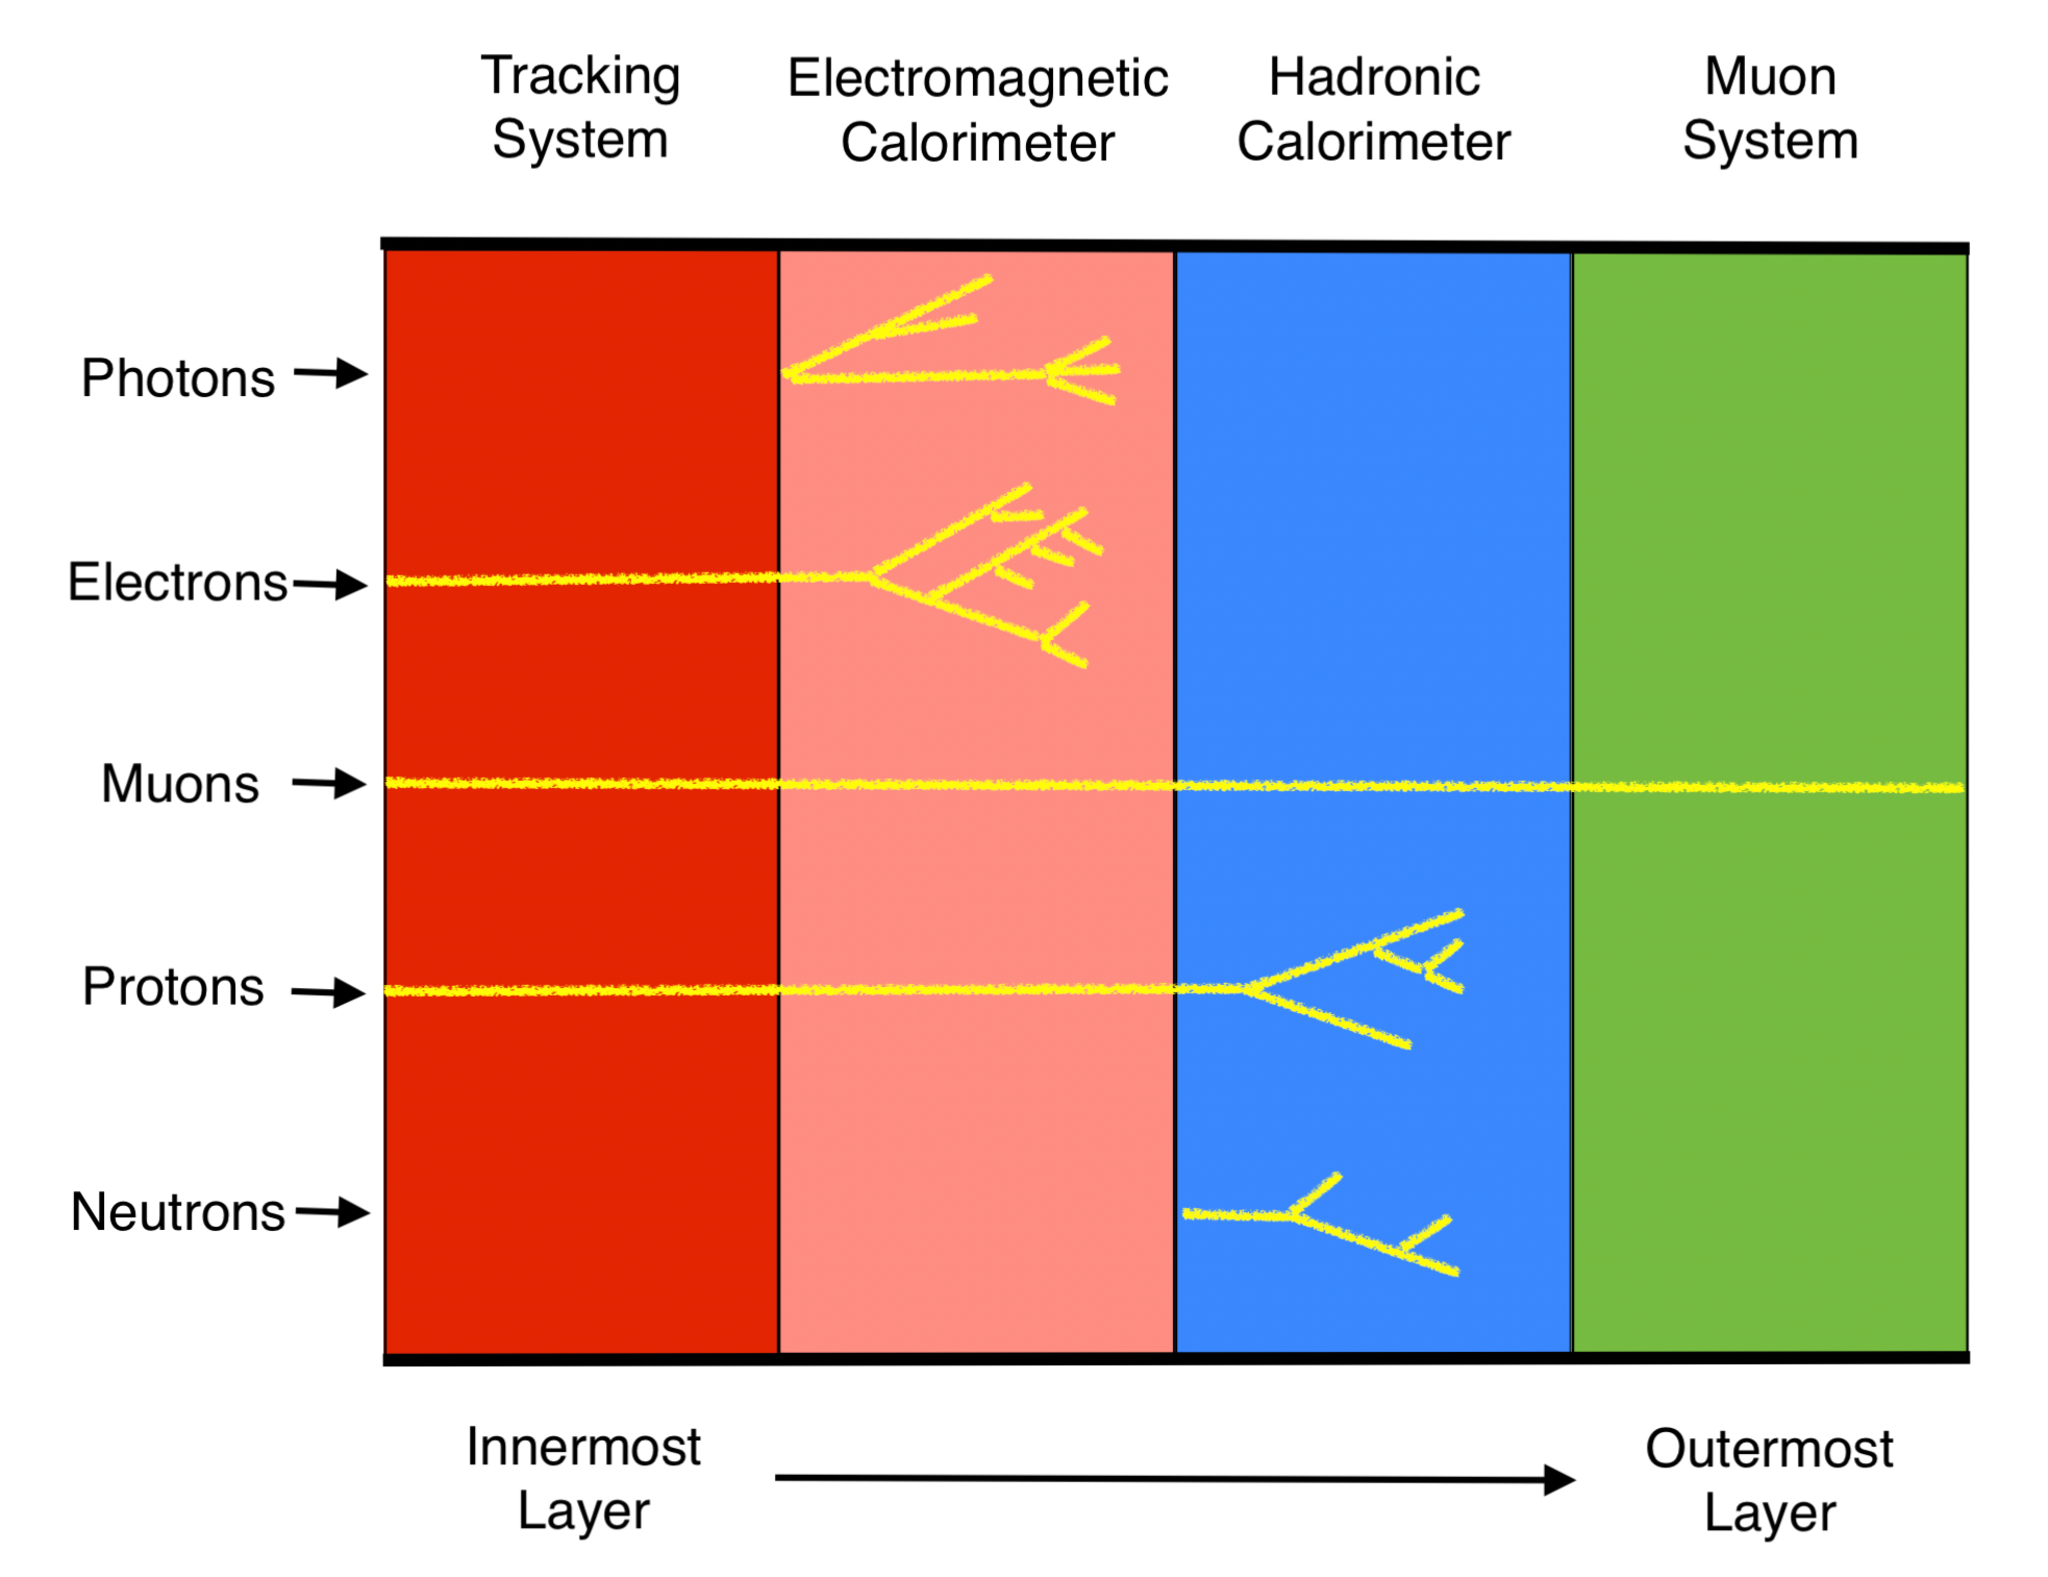
\includegraphics[width=0.7\textwidth]{figures/Chap3/Rizzi-Fig3-4.pdf}
\caption{Components of a typical detector for physics at colliders. Different particles are identified by the distinctive signatures in the subdetectors.}
\label{fig:detector:interaction}
\end{figure}


\subsection{Tracking and spectrometry}
\label{sec:dec:tracking}
A tracking device measures the traces left by charged particles passing through it. To allow the determination of the momentum and the charge of a particle, a tracking device needs to be accompanied by a magnetic field (in this case we speak of a magnetic spectrometer): once the magnetic field is known, the measure of the radius of curvature of the particle is equivalent to a measure of its momentum, according to Equation \ref{eq:cern:p03br}. In a typical particle detector as the one in the schema in Figure \ref{fig:detector:interaction}, both the inner tracking system and the muon system are magnetic spectrometers.

The relative uncertainty in the momentum is given by:
\begin{equation}
\frac{\sigma_p}{p} = \sqrt{ \left(a p \right)^2 + b^2} \; .
\label{eq:tracking:reso}
\end{equation}

The first term, whose relative importance increases for high-momentum particles, derives from the resolution in the measurement of the curvature. Typical values for $a$ are between 0.01\% and 1\%. The constant term in Equation \ref{eq:tracking:reso} accounts for the impact of multiple Coulomb scattering, which broadens the distribution of the transverse momentum perpendicular to the direction of motion. This terms is important only at low energies, while it is negligible for high-energy particles.

There are three main configurations of magnetic fields typically used in momentum spectrometers:
\begin{itemize}
\item A dipole field leads to a rectangular symmetry; if we think of a circular collider with a coordinate system where $z$ is the direction along the beam trajectory and ($x$,$y$) define a Cartesian system in the transverse plane, a dipole  field in the $x$ direction will cause a deflection in the ($y,z$) plane. This is the configuration adopted by forward spectrometers like LHCb, where the tracking devices are arranged in sequence in the $z$ direction. As an example, the integral of the LHCb dipole field over the detector length is 4 Tm.

\item A solenoidal field leads to a cylindrical symmetry and, if the field lines are along the $z$ direction, the deflection is in the ($x,y$) plane. This is the typical configuration of the spectrometers in the central barrel, where the detectors are arranged in cylindrical layers. The CMS solenoid field is 4 T, while the \gls{atlas} one is 2 T. 

\item A toroidal field leads to an azymuthal symmetry: the direction of the field lines is a circle in the transverse plane, and the deflection is in the ($r,z$) plane. This configuration is adopted by the \gls{atlas} muon spectrometer, with a magnetic field of 4 T. As in the case of the solenoidal field, the detectors are arranged in cylindrical shells.
\end{itemize}

The track left by a charged particle curving because of the magnetic field is reconstructed by the tracking detectors. The two most common categories of tracking devices are gas and silicon detectors, described in the next two sections.

\subsubsection*{Gas detectors}

In gas detectors, the passage of a charged particle ionizes the atoms and creates electron-ion pairs. Once the electron and the ion are created, they can be separated (thus creating a current) by applying an electric field. This induces signal on an electrode added to the material, read through a readout system. The basic principle of most of gas detectors relies on a tube with a wire in the center, which is an anode with a high electric field. When the particle crosses the gas, the ionization electrons drift toward the anode and can be collected. 
Without an electric field, the electron and ion would move in the system by thermal diffusion. The effect of an electric field is to make the electron and ion move in opposite directions, allowing us to measure them. Since not many electrons are produced in gas, they need to be amplified. Inside the tube, the electric field decreases with the inverse of the distance from the anode wire. When the electrons reach a distance of a few micrometers from the wire, the electric field is very large and the electrons gain more energy than the ionization energy; this leads to secondary ionization and an exponential growth of the number of electron-ion pairs (avalanche effect). 

Several types of gas detectors with different characteristics have been developed. In single-wire proportional chambers, like the one used in the outer tracker of the LHCb experiment, several counters are combined next to each other, to allow the measurement of the particle position. In multi-wire proportional chambers \cite{CHARPAK1968262} several wires in two perpendicular directions are contained in the same box filled with gas. 
Drift chambers are a further evolution of wire chambers, where the position of the particle is computed by measuring the time taken by the 
secondary ionization to reach the anode. Time projection chambers (TPC) are a different type of gas detector, used for example in ALICE. 
It is constituted by a large area filled only with gas, without wires, with detectors and readout structure only at the end plates. 
Between the plates a strong electric field causes the electron-ion pairs to drift, 
until they reach the plates where a combined measurement of the position and time of arrival allows to reconstruct the three-dimensional 
trajectory of the particle (that can be curved if a magnetic field is added). 
Micro-strips chambers \cite{OED1988351} are more modern, very condensed and thin gas detectors. 
Instead of being generated by a wire, the electric field comes from small metal deposits on a high-resistivity substrate.   

In general the main problems of gas detectors based on ionization are the spatial extension and the long drift time, 
which nevertheless make them suitable for the outer part of the \gls{lhc} detectors, in particular muon spectrometers.

All the gas detectors described above are based on the electron-ion pairs created by the ionization induced by the charged particle. A different principle is used in \gls{trd}. \glspl{trd} are based on detecting the electromagnetic radiation emitted by particles that cross boundaries between different media below the Cherenkov threshold \cite{1402-4896-1982-T2A-024}. The energy radiated increases with the energy of the incoming particle. These detectors are less common for tracking, but are mentioned here as the main example of a modern \gls{trd} in high-energy physics is the \gls{trt} in the inner detector of the \gls{atlas} experiment.

\subsubsection*{Solid-state detectors}

Semiconductor (and in particular silicon) detectors are the main type of solid-state detectors, and are currently the most used for inner tracking, 
where high precision and low occupancy are needed \cite{Hartmann:2009zza}. 
These detectors detectors are also based on the ionization of the material but in this case, since the structure is a crystal, 
we talk about electrons and electron holes. 

The underlying principle is based on the band model of solids, describing the allowed energy levels for electrons in a solid: when many atoms of the same type are bound together in a crystal lattice, in order to fulfill Pauli's principle the atomic orbitals split into many closely spaced molecular orbitals, that can be considered as continuous energy bands. The highest-energy full band is the valence band, while the lowest partially-filled (or empty) band is the conduction band; the energy difference between the conduction band and the valence band is referred to as energy gap. 


Semiconductors are materials where the conduction band is almost empty, but the energy gap is small ($\approx$ 1 eV, e.g. 1.07 eV for silicon), so the conduction band can be occupied by excited electrons from the valence band; this leaves holes in the valence band, that under the effect of an electric field can drift as well. Semiconductors with a pure composition have the same amount of electrons and holes. If the semiconductor is doped with an atom with one more electron in the valence band, this creates an excess of electrons and the material is referred to as a n-type semiconductor. If instead the impurities are electron acceptors, the material has an excess of holes and is referred to as p-type semiconductor. When a p-type and a n-type semiconductors are pulled together, the holes of the p-side drift into the n-side, and the electrons from the n-side into the p-side. This creates an electric field that takes charge carriers out of the area where it is present (depletion region). When a charged particle passes through the semiconductor, it produces electron-hole pairs in the depletion region; these drift apart because of the electric field and can be collected by electrodes. The application of a negative potential difference between the p-side and the n-side can increase the depletion area.

The density of silicon is about one thousand times higher than that of gases like argon, and silicon also needs a much lower energy to be ionized (3.6 eV for silicon, while it is about 250 times higher for argon). This leads to a much higher number of electron-holes pairs than the number of electron-ion pairs in gas detectors, so the signal needs very little amplification, and the size of the detector itself can be smaller. 

Different configurations of the silicon sensors are possible. In a single-sided strip sensor, the readout strips are at negative potential. The second coordinate can be determined if also the n-side is divided into strips in a direction orthogonal to the ones in the p-side. 
The grid structure of this double-sided strip sensors can still lead to ambiguities when the number of hits is elevated; a true two-dimensional sensitivity is offered only by the pixel modules, where the module is divided in a matrix-like shape.



\subsection{Calorimetry}
\label{sec:dec:calo}

Calorimeters can determine the energy of both charged and neutral particles through a destructive measurement: the energy of the particles is deposited in the detector material and transformed into a measurable quantity. Because of their sensitivity to a wide variety of particles, good energy resolution and relatively small size, they are very attractive devices for accelerator physics experiments \cite{RevModPhys.75.1243,Wigmans:2000vf}.

When the incident particle interacts with the material of the calorimeter it develops a cascade of particles (shower), with different characteristics for electromagnetic and hadronic interactions, described in the next two sections. Different types of calorimeters are necessary to capture the two typologies. The energy of the shower is decreased by the interactions happening in the absorber material, while the active material provides the conversion of the energy into a charge or light signal. In sampling calorimeters layers of absorber and active material are alternated in sequence, while in homogeneous calorimeters a single material carries out both functions.


\subsubsection*{Electromagnetic calorimeters}

The type of interaction that electromagnetically interacting particles have with the detector depends on their energy. 
%As an example, the photon interaction cross-section in lead is shown in Figure  \ref{fig:det:xsec_photon}. 
%The average fractional energy loss in lead for electrons and positrons and the photon interaction cross-section in lead are shown in Figures \ref{fig:det:xsec_elec:a} and \ref{fig:det:xsec_elec:b} respectively. 

%\begin{figure}[ht]
%\centering
%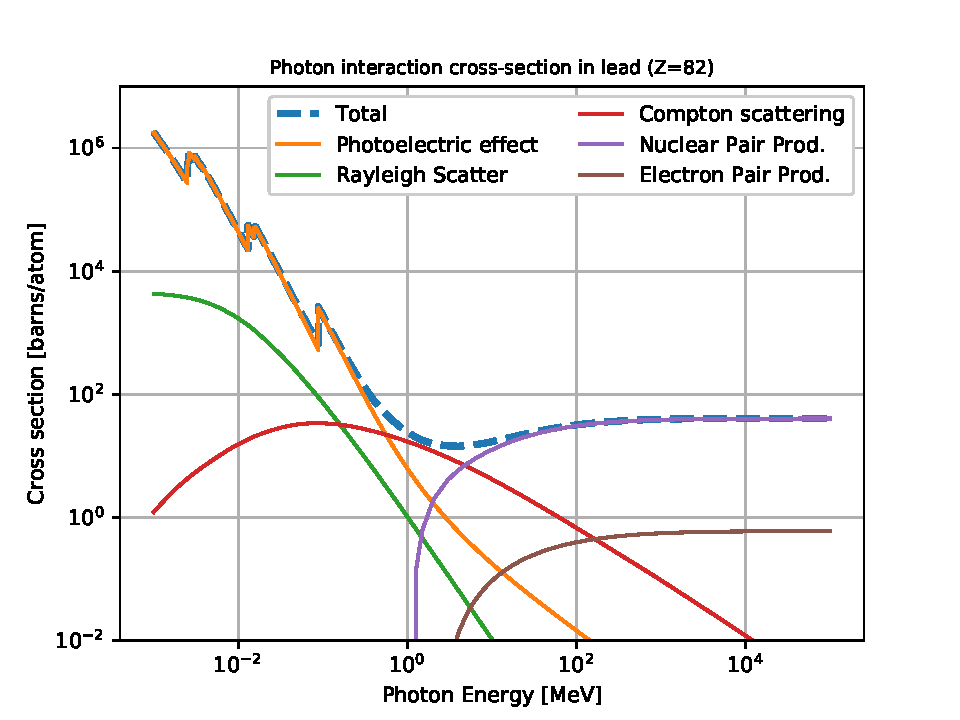
\includegraphics[width=0.54\textwidth]{figures/Chap3/Rizzi-Fig3-5.pdf}
%\caption{Photon interaction cross-section in lead. Numbers from Ref. \cite{Nist}. }
%\label{fig:det:xsec_photon}
%\end{figure}

For photons and electrons with energies above 1 GeV, the dominant type of interaction is nuclear pair production and Bremsstrahlung, respectively. 
When these particles traverse a block of material they produce a cascade of particles (electromagnetic shower): electrons and positrons can emit a photon by Bremsstrahlung, and a photon, thanks to the interaction with a nucleus, can turn into an electron-positron pair.

The main parameter to describe the evolution of an electromagnetic shower is the radiation length ($X_0$), defined as the distance over which an electron reduces its energy to $1/e$ of the initial value, and it corresponds also to 7/9 of the mean free path for pair production for a photon. The radiation length depends on the characteristics of the material:
\begin{equation}
X_0 [\frac{g}{cm^2}] = \frac{716 \frac{g}{ cm^2} A }{Z(Z+1) \ln\left(287/\sqrt{Z}\right)} \; , \nonumber
\end{equation}

\noindent where $A$ and $Z$ are the atomic and mass number of the material. If we define $t = x/X_0$ as the shower depth relative to the radiation length, the maximum number of produced particles occurs at:
\begin{equation}
t_{max} = \frac{\ln\left(E_0/E_c\right)}{ln\left(2\right)} \;. \nonumber
\end{equation}
Typical values for the radiation length are of the order of the cm (e.g. 0.56 cm for lead, 1.76 cm for iron \cite{Patrignani:2016xqp}); 99\% of the shower is contained in about 11(22) $X_0$ for a particle with an energy of 1 GeV(TeV), 
allowing for electromagnetic calorimeters of compact dimensions. 
The lateral width of the shower, determined mainly by multiple scattering, increases with depth and is defined in terms of the Moli\`ere radius:
\begin{equation}
R_M = \frac{21 MeV \; X_0[\frac{g}{cm^2}]}{E_c [MeV]} \; . \nonumber
\end{equation}

\noindent A cylinder of radius 2$R_M$ contains about 95\% of the shower; for most calorimeters $R_M$ has a value of few centimeters, so electromagnetic showers are quite narrow. 

Once the electrons in the shower have an energy lower than the critical energy 
($E_c$, defined as the energy where the loss through Bremsstrahlung equals the loss through ionization), 
the shower stops as the energy is dissipated mostly through ionization for electrons and photoelectric effect for photons, 
and no longer through the creation of new particles. 
Therefore all the energy of the incoming particle is in the end used to ionize the material of the detector, and this is the effect that is detected.


We have discussed in Section \ref{sec:dec:tracking} how the resolution of the momentum measurement in a magnetic spectrometer decreases with the increase in the momentum itself. Instead, the relative energy resolution in a calorimeter improves for high-energy particles, and can be written in the parametric form:

\begin{equation}
\frac{\sigma_E}{E} = \sqrt{\left(\frac{a}{\sqrt{E}} \right)^2 + \left( \frac{b}{E} \right)^2 + c^2 } \; . \nonumber
\end{equation}

\noindent The first term of the sum in quadrature reflects the stochastic nature of the shower development: ignoring the instrumental effects, the energy resolution of a calorimeter is proportional to the square root of the total track length, which is in turn proportional to the initial energy. The contribution of this term is small in homogeneous calorimeters, while is larger in sampling calorimeters (because of fluctuations in the fraction of energy deposited in the absorber) and it grows with the thickness of the absorber layers; typical values for $a$ are 5-20\% if the energy is expressed in GeV. The second term is the noise term originating from the electronic noise of the readout chain; this term is in general more relevant for calorimeters producing charge signals than for those producing light signals, and can become the dominant term for particles with energy below 1 GeV. The last term is a constant deriving from instrumental effects that produce a non-uniform detector response, including for example energy lost outside the detector volume and radiation damage; this becomes the dominant term at high energies and is typically $<1\%$. 



\subsubsection*{Hadronic calorimeters}

The difference between electromagnetic calorimeters and hadronic calorimeters finds its origin in the more complicated nature of strong interactions compared to the electromagnetic ones. 

%A sketch of the evolution of a hadronic shower is shown in Figure \ref{fig:det:shower_had:a}. 
With respect to electromagnetic showers, hadronic ones have a much larger spatial extension. On the longitudinal direction, the scale is determined by the nuclear interaction length ($\lambda_I$), which is material-dependent and can be expressed as:
\begin{equation}
\lambda_I = 35 \frac{g}{cm^2} A^{1/3} \; , \nonumber
\end{equation}

\noindent where $A$ is the atomic number of the material. For most materials used in particle detectors this turns out to be larger than $X_0$ (e.g. the nuclear interaction length is 17.59 cm for lead, and 16.77 cm for iron \cite{Patrignani:2016xqp}). The 99\% shower containment is reached after about 5(9) $\lambda_I$ for pions with E=10(138) GeV. Also the lateral width of the shower is larger than in electromagnetic interactions: while the size of the Moli\'ere radius is determined mainly by multiple scattering, the lateral profile of a hadronic shower depends on the transverse-momentum transfer, which can be quite sizable in strong nuclear interactions. 
%Figure \ref{fig:det:shower_had:b} shows the lateral shower profile in iron for pions with E=10 GeV.

%\begin{figure}[ht]
%\centering
%\subfigure[]{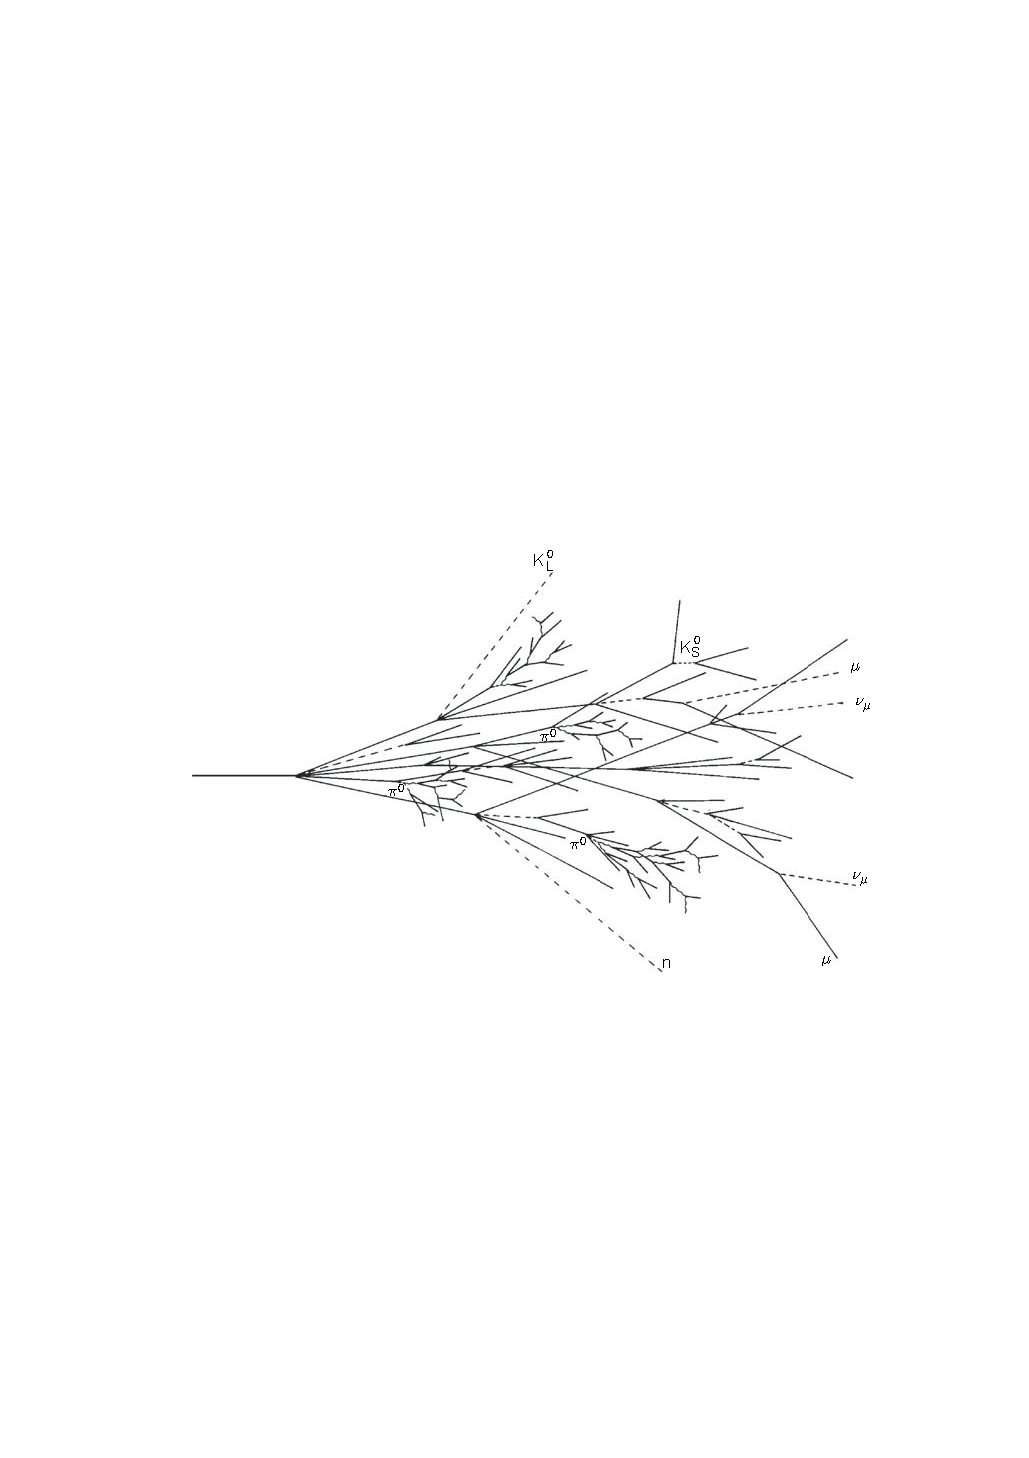
\includegraphics[width=0.48\textwidth]{figures/Chap3/Rizzi-Fig3-6-1.pdf}\label{fig:det:shower_had:a}}
%\subfigure[]{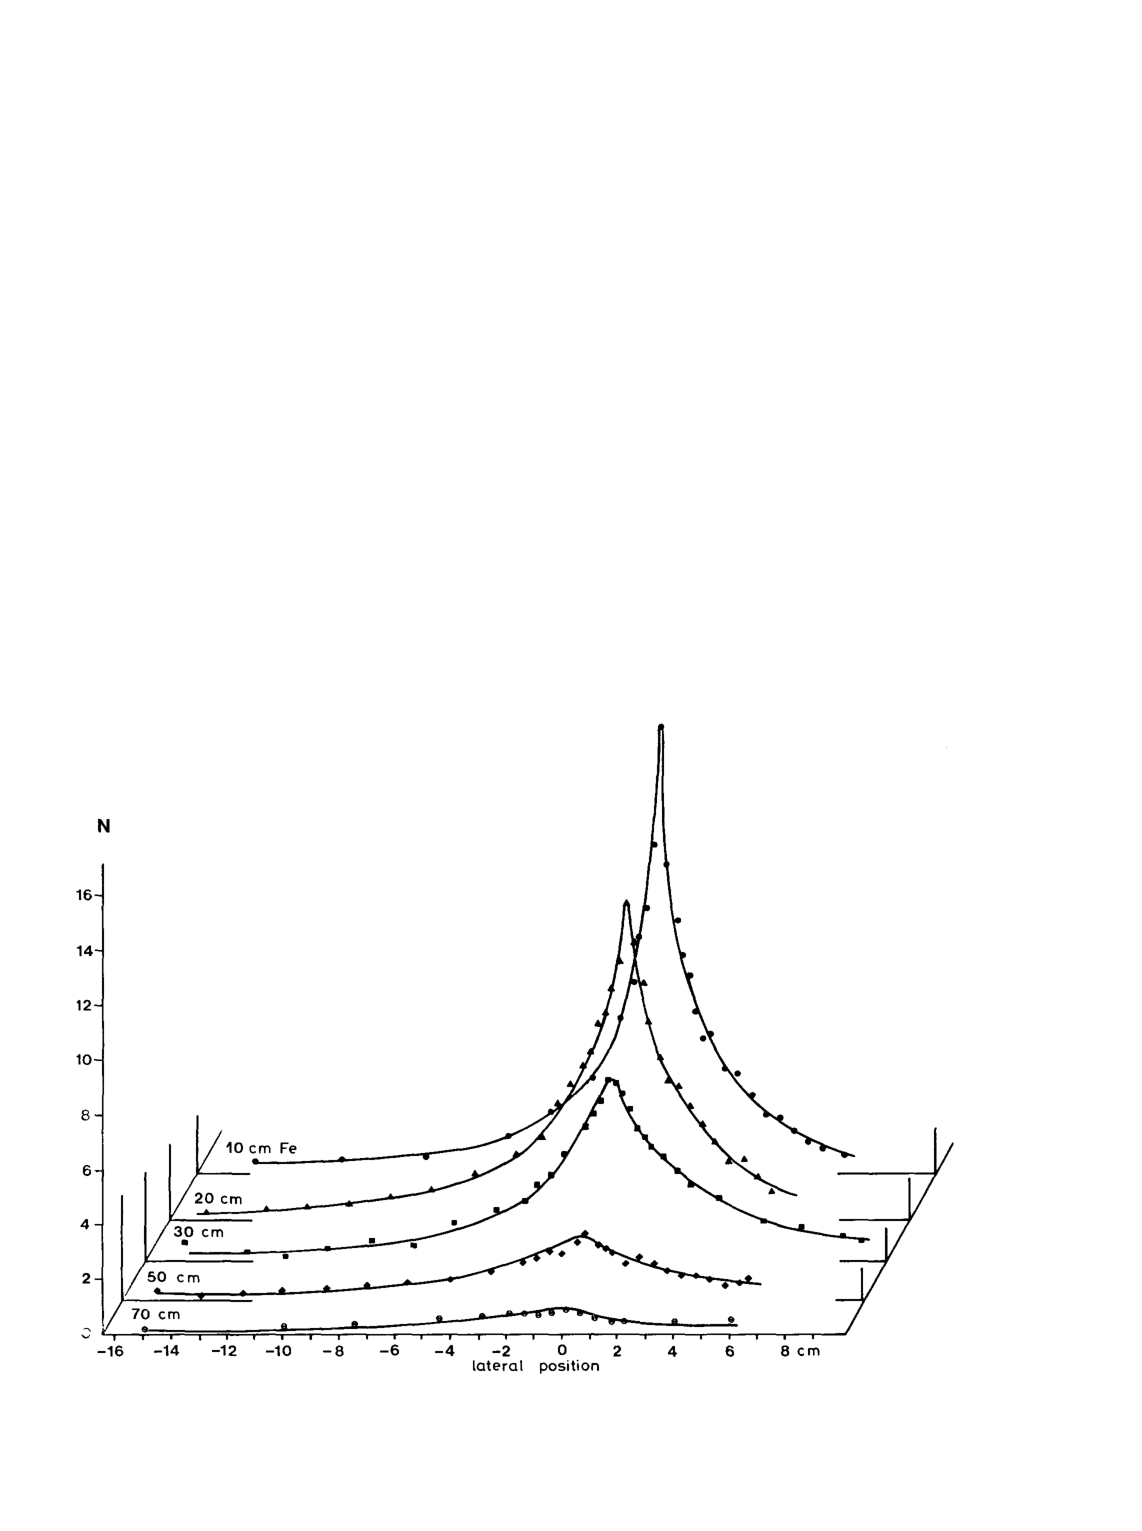
\includegraphics[width=0.48\textwidth]{figures/Chap3/Rizzi-Fig3-6-2.pdf}\label{fig:det:shower_had:b}}
%\caption{\subref{fig:det:shower_had:a} Sketch of the evolution of a hadronic shower. Figure from Ref. \cite{grupen_shwartz_2008}. 
%\subref{fig:det:shower_had:b} Lateral energy distribution of shower induced by $\pi^-$ with E=10 GeV, measured at a depth of 10, 20, 30, 50 and 70 cm in Fe. Figure from Ref. \cite{FRIEND1976505}.}
%\label{fig:det:shower_had}
%\end{figure}


Another difference with electromagnetic showers lies in the composition of the shower: while an electromagnetic shower is constituted only by electrons, positrons and photons, a much larger variety of particles participates in hadronic showers, including both hadrons and electromagnetically-interacting particles. Starting from the simplifying assumption that one third of the particles produced in nuclear interactions are neutral pions ($f_{\pi^0}=1/3$), a first approximation of the electromagnetic fraction of a shower is given by:
\begin{equation}
f_{em} = 1 - \left(1 - \frac{1}{3} \right)^n \; , \nonumber
\end{equation}
where $n$ is the number of generations in the shower. Since the number of generations increases with the initial energy, it is intuitive that also $f_{em}$ will be larger for particles of higher energy. It is found \cite{GABRIEL1994336}:
\begin{equation}
f_{em} = 1 - \left(\frac{E}{E_0}\right)^{k-1} \; , \nonumber
\end{equation}
where $E_0$ is the energy necessary to produce one pion (e.g. 0.7 GeV for iron and 1.3 GeV for lead), and $k$ is a slope parameter related to $f_{\pi^0}$ through the average multiplicity ${<}m{>}$:
\begin{equation}
1-f_{\pi^0} = {<}m{>}^{k-1} \;. \nonumber
\end{equation}


%\begin{figure}[ht]
%\centering
%\subfigure{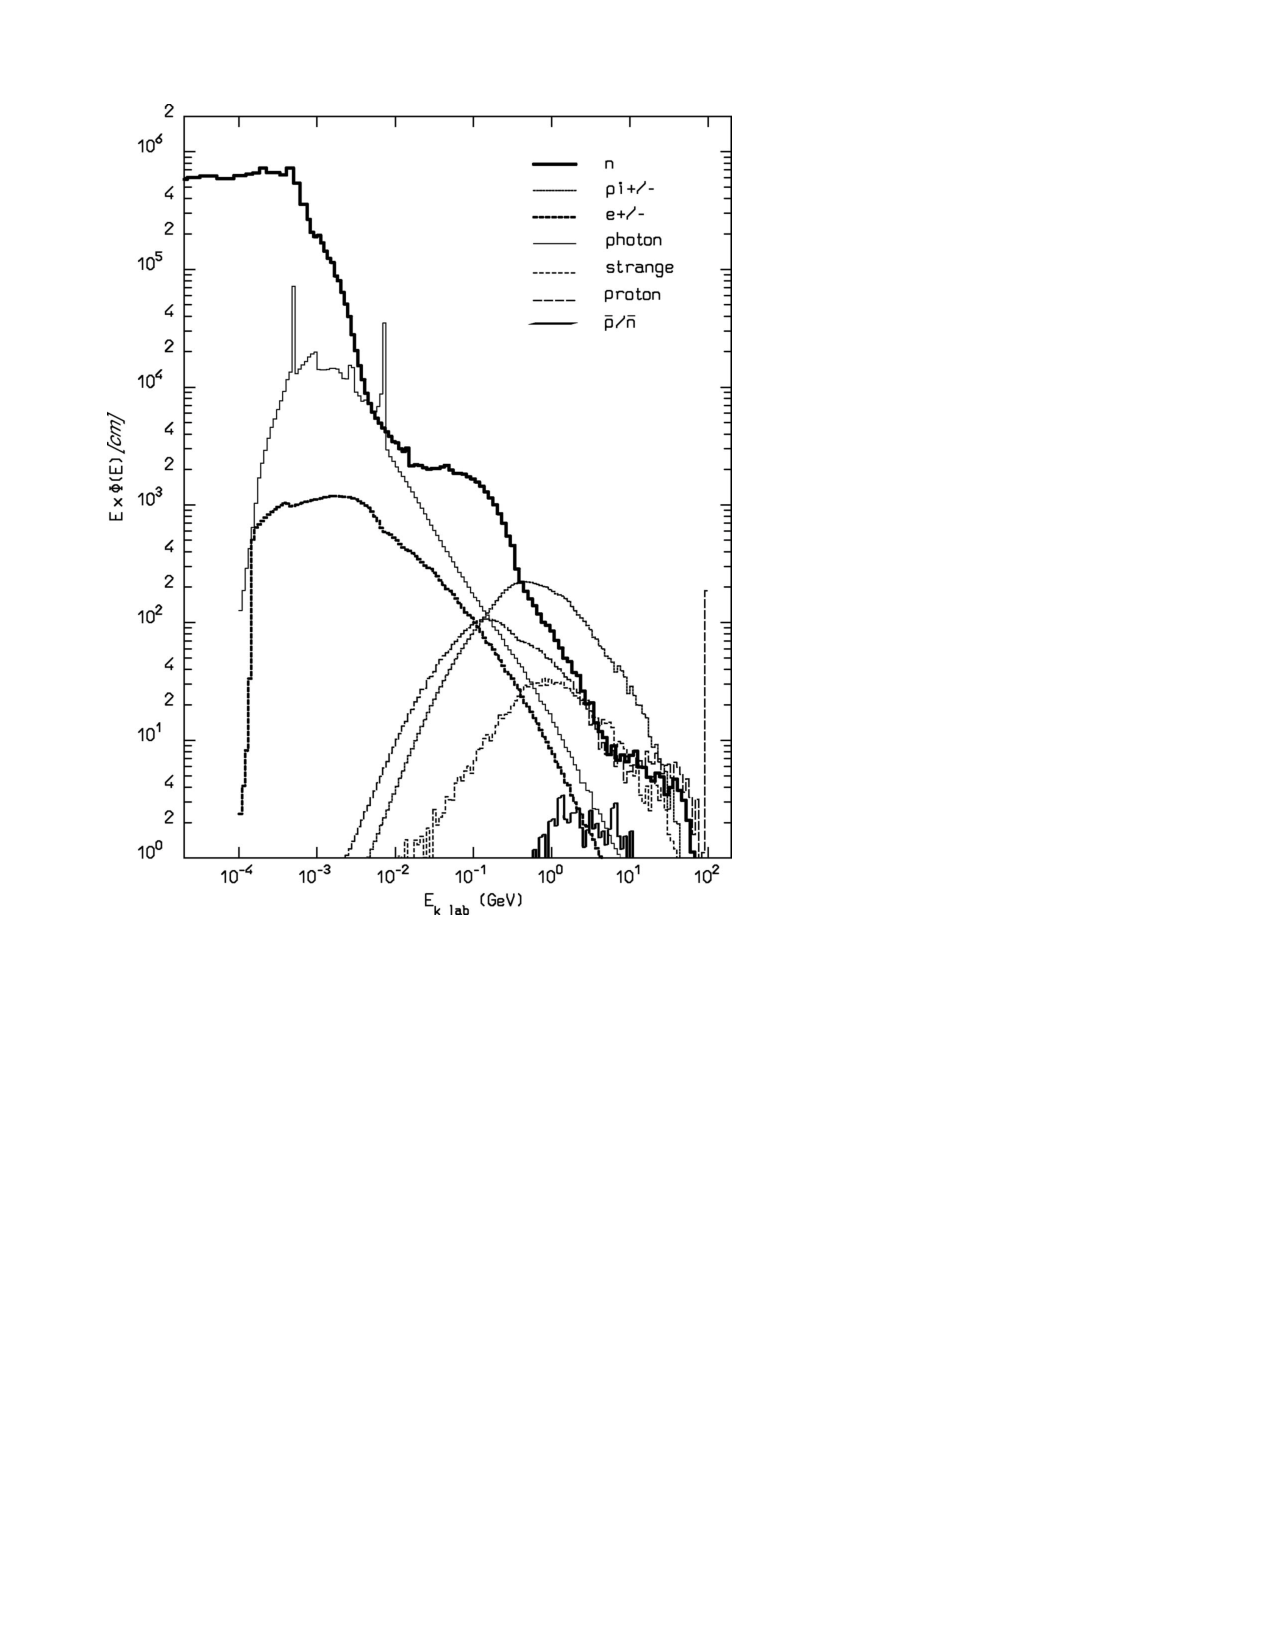
\includegraphics[width=0.42\textwidth]{figures/Chap3/Rizzi-Fig3-7-1.pdf}}
%\caption{Particle spectra produced by protons with E=100 GeV absorbed by lead, as simulated by the Fluka code \cite{Ferrari:898301} and averaged over many showers. Figure from Ref. \cite{RevModPhys.75.1243}.}
%\label{fig:det:shower_had_spectra}
%\end{figure}

%Figure \ref{fig:det:shower_had_spectra} shows 

If we consider e.g. the particle spectra produced by protons with E=100 GeV absorbed by lead, at low energies the particle content is dominated by electrons, positrons, photons and neutrons \cite{RevModPhys.75.1243}.

While in electromagnetic showers most of the initial energy is recorded in the detector, in hadronic showers a relevant fraction (up to 30-40\%) is invisible. This invisible fraction is caused by energy that goes into breaking the nuclear bonds, nuclear fragments that in sampling calorimeters do not reach the active material, and neutral particles that can escape the calorimeter (e.g. neutrinos or long-lived neutral kaons). Therefore, for the same initial energy, the visible energy will be lower for a hadronic shower than for an electromagnetic one. If we define the response as the collected signal per unit of incident energy, the invisible energy causes a different response of calorimeters to the electromagnetic and to the purely-hadronic parts of the shower. Defining $R_{em}$, $R_{h}$, $R_{\pi}$ respectively as the calorimeter response to electromagnetic shower, the hadronic part of the shower and to pions, we have that:
\begin{equation}
R_{\pi} = f_{em}R_{em} + (1-f_{em}) R_h = R_h \left( \frac{R_{em}}{R_{h}}f_{em} + (1-f_{em})  \right) \; . \nonumber
\end{equation}

In general, it is expected that $R_{em}/R_{h}>1$. Since the value of the electromagnetic fraction is energy-dependent, the signal from the calorimeter does not increase linearly with energy. Compensating calorimeters are aiming at having the same response to the electromagnetic and hadronic part of the shower ($R_{em}/R_{h}=1$), restoring the linearity of the calorimeter response. In non-compensating calorimeters the fluctuations in $f_{em}$ are the dominant component of the energy resolution and, since the fluctuations are approximately Gaussian,
they give rise to a term proportional to:

\begin{equation}
\frac{\sigma_E}{E} = \frac{\mathrm{const}}{\sqrt{E}}  \; . \nonumber
\end{equation}
In modern non-compensating calorimeters the value of the constant is about 0.4, while it can be as low as 0.2 in the case of compensating calorimeters.


\subsection{Detecting photons}

As already mentioned in previous sections, photons are often the result of the passage of a particle through the material; 
this is the case e.g. in \glspl{trd} or in calorimeters with scintillator as active material. 
This sections gives an overview of how these photons can generate a detectable current; for a more extensive discussion see e.g. Ref. \cite{lightdetection,Grupen:2012zpa}. The typical process of photon detection can be summarized in three different steps: (1) the incident photon generates a photoelectron or an electron-hole pair through the photoelectric or photoconductive effect, (2) the signal of the photoelectron is  
amplified, and (3) the amplified signal is collected. Important properties to classify photon-detecting devices are \cite{Patrignani:2016xqp}:
\begin{description}
\item[Quantum efficiency:] The probability that the incident photon generates a photoelectron. This depends on the photon wavelength.
\item[Collection efficiency:] The probability that the photoelectron is collected at the end of the chain.
\item[Photon detection efficiency:] The product of quantum and collection efficiency.
\item[Gain:] The amplification of the photoelectron, quantified as the number of electrons collected for each photoelectron generated.
\item[Dark current or dark noise:] The output current in the absence of signal.
\item[Energy resolution:] Resolution depending on electronic noise and statistical fluctuations.
\item[Dynamic range:] Maximum intensity that the detector can handle expressed in units of the smallest intensity with a signal-to-noise ratio above one.
\item[Time dependence:] Time between the arrival of the photon and the collection of the electrical current.
\item[Rate capability:] Inverse of the time needed after the arrival of a photon to be ready for another one.
\end{description}

Photon detectors can be broadly classified into three categories: vacuum, gaseous and solid-state detectors, described in the following paragraphs.

\subsubsection*{Photomultiplier tubes}  

\Glspl{pmt} are the most common type of vacuum photon detectors. 
A sketch of the structure of a \gls{pmt} is shown in Figure \ref{fig:det:pmt}. It consists of a vacuum tube with an input window, a photocatode, 
a focusing electrode, electron multipliers, and an anode  \cite{hamamatsu}. 
Photons enter the device through the window and excite the electrons in the valence band of the photocatode, which is a semiconductor; 
in transmission-type \glspl{pmt} the photocatode is deposited on the inside of the window, 
while in reflection-type \glspl{pmt} it is on a separate surface. 
The excited electrons diffuse to the surface of the semiconductor and, if they have enough energy to overcome the vacuum level barrier, 
are emitted as photoelectrons. These are accelerated and focused by the electrode toward the multi-stage dynodes, 
a system of electrodes coated with a secondary emissive material, 
where the incident electrons are multiplied. 
The gain $G$ of the \gls{pmt} depends on the applied voltage $V$ as $G=AV^{kn}$, 
where $A$ and $k$ are constants and $n$ is the number of multiplicative stages. 
Typical values for the gain are $10^5-10^6$. After the last stage of multiplication, the electrons are collected by the anode, 
which then outputs the current to the external circuit.

\begin{figure}[ht]
\centering
\subfigure{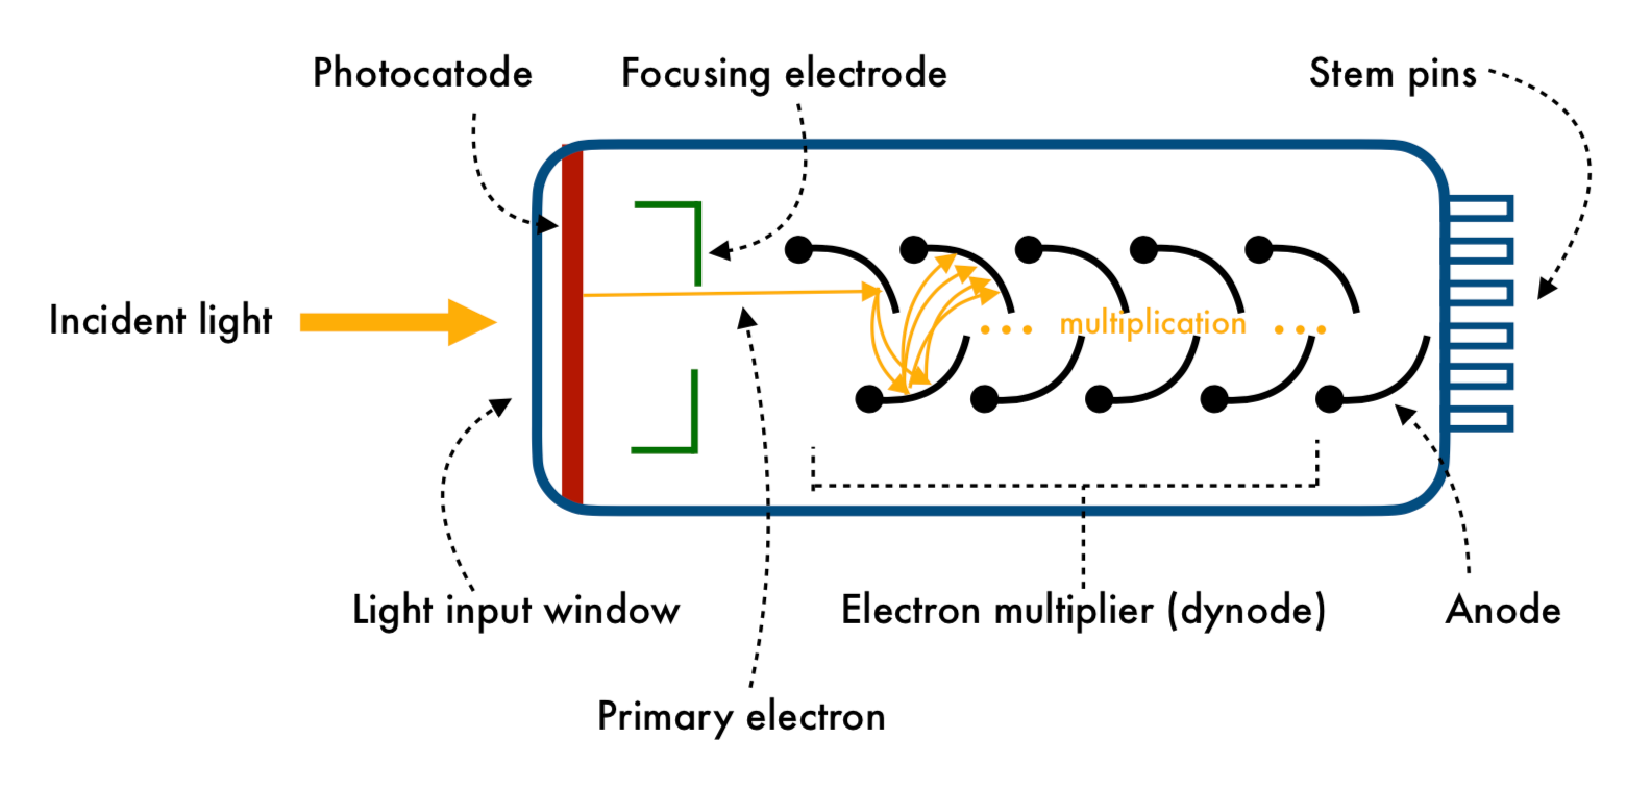
\includegraphics[width=0.8\textwidth]{figures/Chap3/Rizzi-Fig3-8-1.pdf}}
\caption{Sketch of the structure of a \gls{pmt}. }
\label{fig:det:pmt}
\end{figure}

Beside \glspl{pmt}, other examples of vacuum photon detectors are \gls{mcp} and \gls{hpd}. \glspl{mcp} are based on the same principle as \glspl{pmt} but substitute the discrete multiplicative stages of the dynodes with continuous multiplication in cylindrical holes of a few $\mu$m. The decreased size of a \gls{mcp} comes at the price of a large recovery time, shorter lifetime and smaller gain (typically $\approx 10^4$). In \glspl{hpd} photoelectrons are accelerated onto a silicon sensor, allowing higher resolution in space and energy; this type of sensors are used e.g. in the \gls{cms} hadronic calorimeter.

\subsubsection*{Gaseous photon detectors}
In gaseous photon detectors the photoelectrons are multiplied through the avalanche effect in an high-field region, similarly to what happens in gaseous tracking detectors. The photoelectrons are generated by the interaction of the photon either with a solid photocatode or with a photosensitive molecule vaporized and mixed in the gas itself. 

\subsubsection*{Solid-State photon detectors}
Solid state photon detectors are devices where the production and detection of the photoelectrons takes place in the same semiconductor material. They are in rapid development (see e.g. Ref. \cite{Renker:2009zz}) as they provide a smaller, and often cheaper, option to \glspl{pmt} and gaseous detectors, especially when the area to be covered is small. 
Silicon photodiodes are devices based on a reverse-biased p-n junction, used in many applications from high-energy physics to solar cells. 
Photons passing through the silicon create electron-hole pairs through the photoconductive effect, which are then collected respectively at the positive and negative side of the chip. 

 %Advances in solid state photon detectors




%%%%%%%%%%%%%%%%%% ATLAS

\section{The ATLAS experiment}
\label{sed:cern:atlas}

\gls{atlas} \cite{atlas:atlas}, shown in Figure \ref{fig:atlas:atlas}, is the largest of the \gls{lhc} detectors, 
measuring 44 meters in length and 25 meters in height, and weighting about 7000 tons. 
To be fully functional in the \gls{lhc} environment,  the \gls{atlas} detector needs to be fast in order to resolve the collisions resulting from consecutive bunches (which are interspaced by 25 ns) and radiation resistant. 

\begin{figure}[ht]
\centering
\subfigure{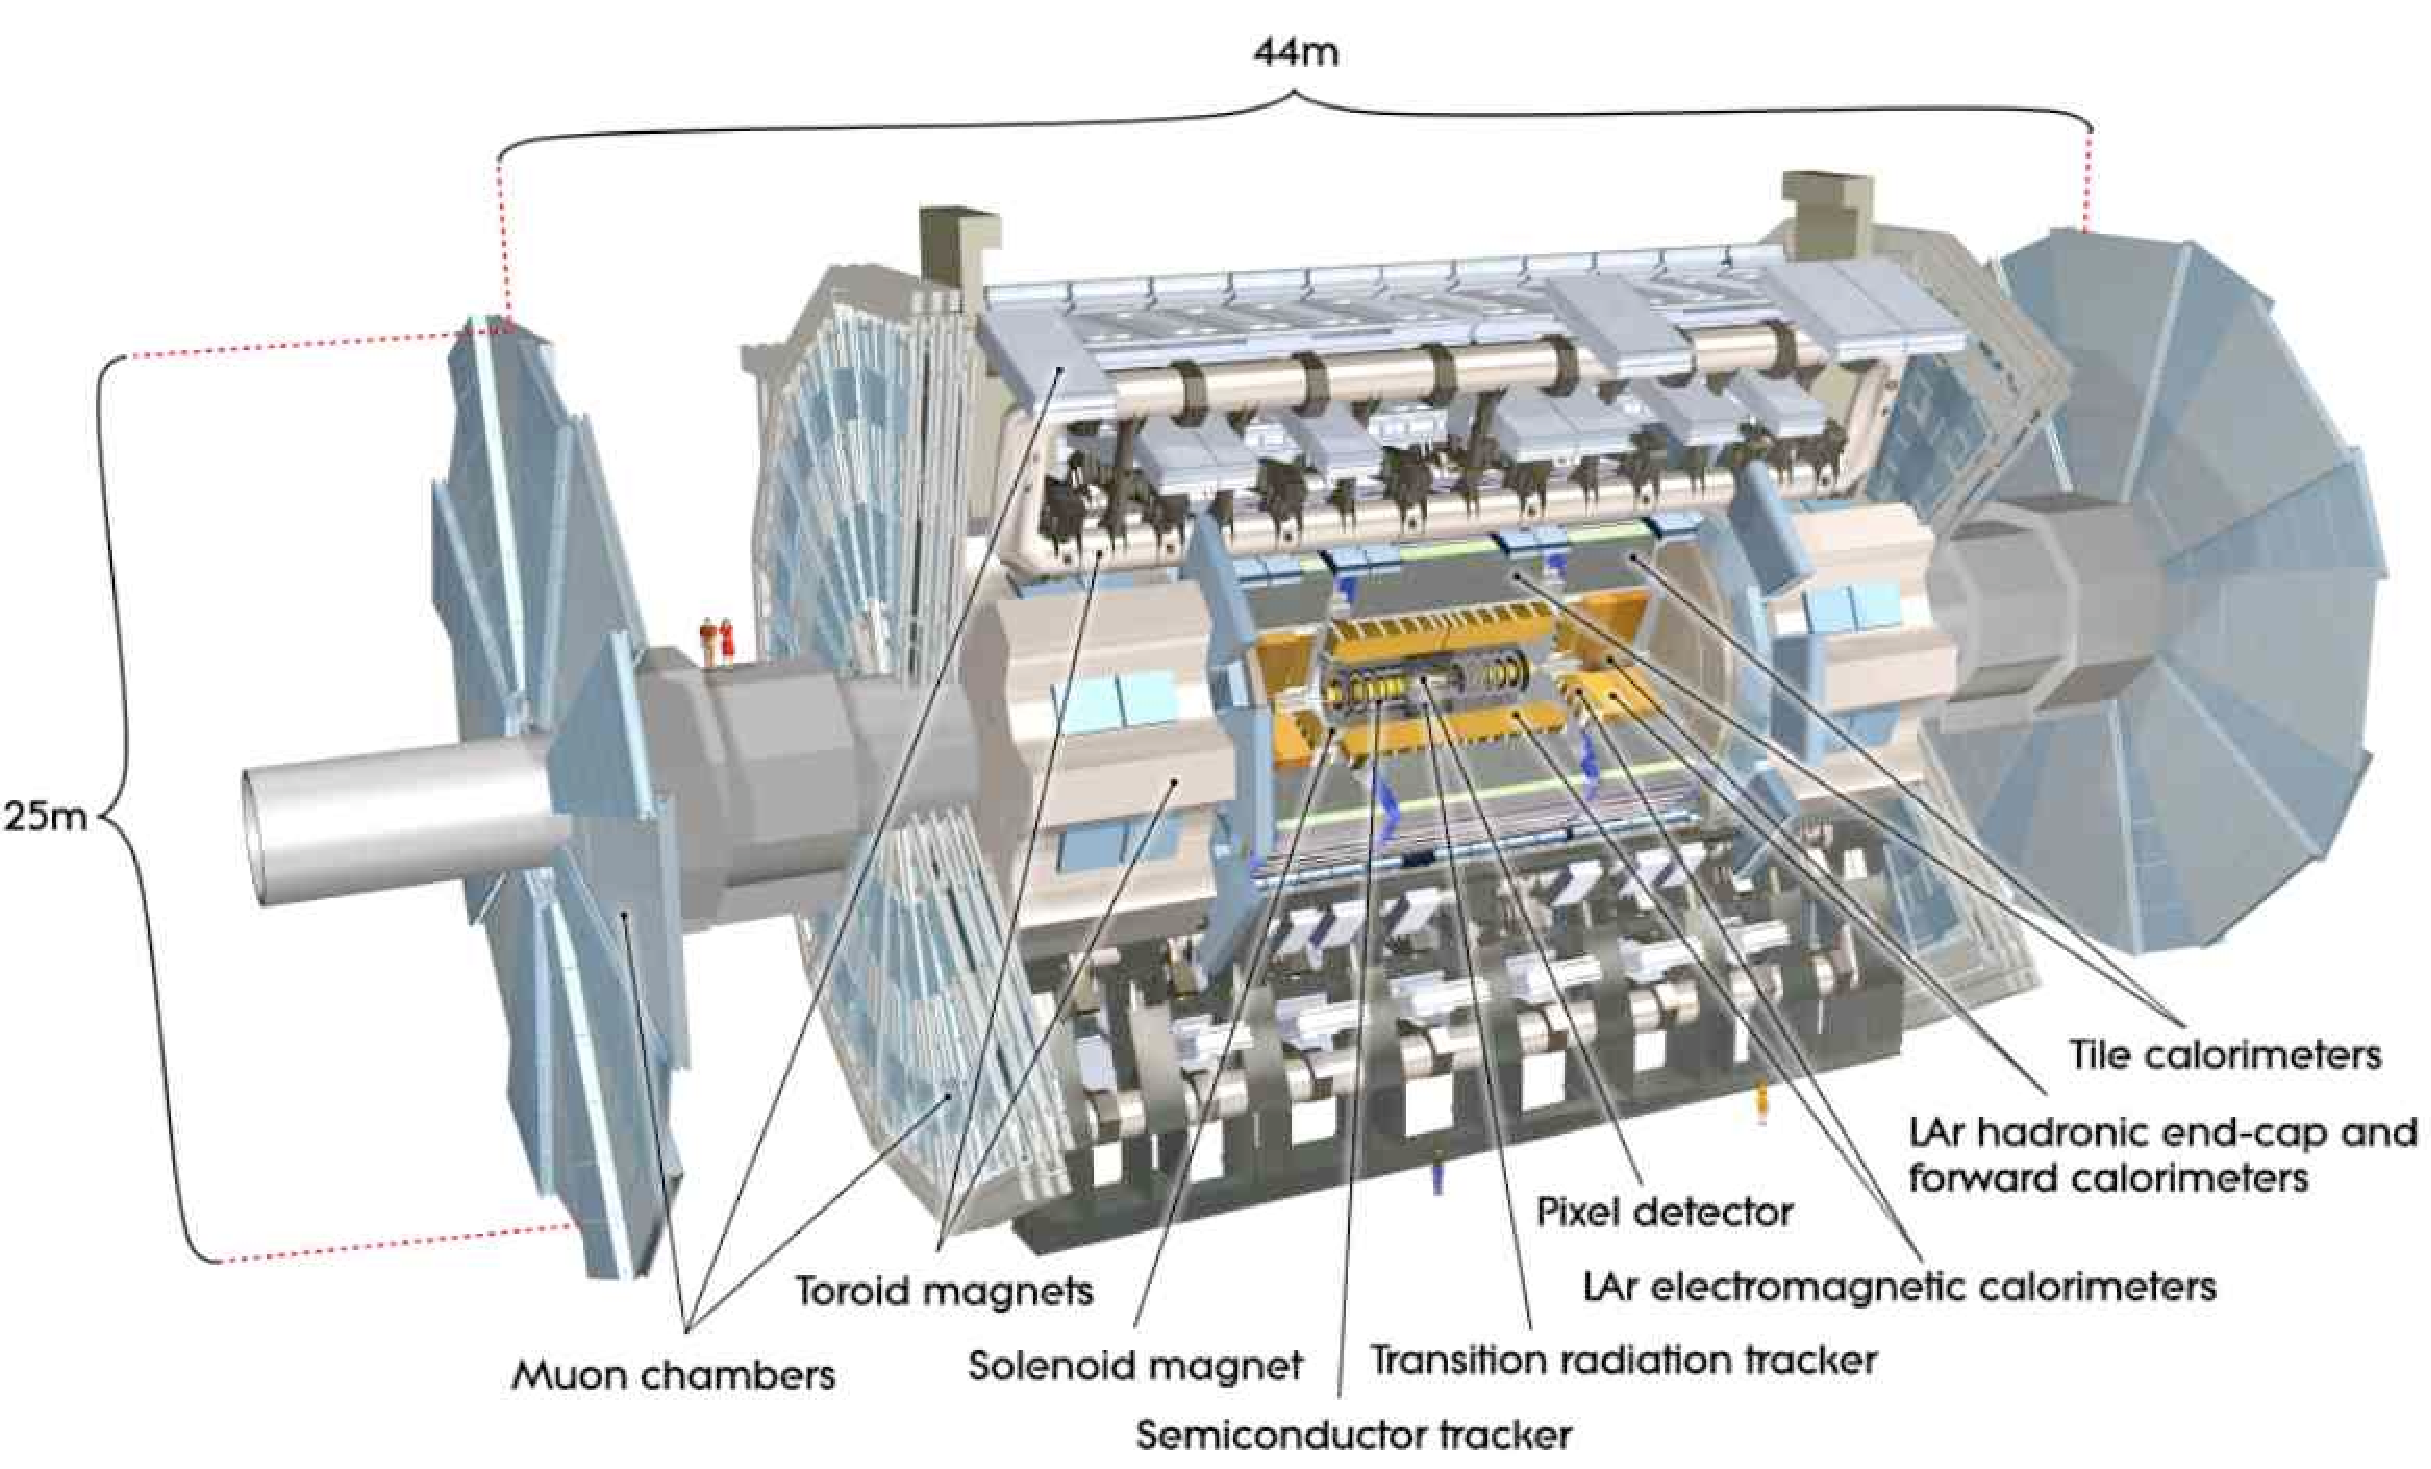
\includegraphics[width=0.85\textwidth]{figures/Chap3/Rizzi-Fig3-9-1.pdf}}
\caption{Drawing of the \gls{atlas} detector showing the different subdetectors and
the magnet systems. Figure from Ref. \cite{atlas:atlas}.}
\label{fig:atlas:atlas}
\end{figure}

The \gls{atlas} physics program covers a large variety of topics: 
\begin{itemize}
\item \gls{sm} processes can be measured at the \gls{lhc} at energies never reached before, and being sensitive to them is essential both to provide accurate measurements and to use them as candles to calibrate the detector. 
\item The discovery of the Higgs boson was one of the main goals of the \gls{lhc} and, after its observation in 2012, the focus moved onto measuring its properties. 
\item Compared to the Tevatron, the \gls{lhc} is a true top-quark factory, 
and the study of the properties of this particle can both probe the \gls{sm} and set limits on \gls{bsm} theories.
\item The \gls{lhc} offers an exciting opportunity to discover \gls{bsm} physics, and \gls{atlas} needs to be ready to identify its signs. 
\item \gls{atlas} has a dedicated program to study the properties of the physics involving \textit{b}- and \textit{c}-quarks, and of the physics of low mass states.  
\item \gls{atlas} also carries out a heavy-ion program.
\end{itemize}

To cope with the wide range of types and energies (from few GeV to several TeV) of particles that need to be identified, \gls{atlas} relies on a sequence of subdetectors nested in a cylindrical geometry, that follow the general schema discussed in Section \ref{sec:detectors:identification}: close to the \gls{ip} we find the \gls{id}, embedded in a solenoidal magnetic field of 2 T. The following layers are the \gls{ecal} and \gls{hcal}, and the outermost part is occupied by the muon system, where muons are bent by a 4 T toroidal magnetic field. All these components are described in the next sections.

\subsection{Coordinate system}

\gls{atlas} uses a right-handed coordinate system, with its origin at the nominal \gls{ip}. The $z$-axis follows the beam direction, 
while in the transverse plane the $y$-axis points upward and the $x$-axis toward the \gls{lhc} center. Positive and negative values of the $z$-axis identify respectively the A-side and the C-side of the detector. 
When spherical coordinates are used, the azimuthal angle $\phi$ is defined starting from the $x$-axis, 
and ranges between $-\pi$ and $\pi$; the polar angle $\theta$ is defined starting from the $z$-axis and takes values between $0$ and $\pi$. 
The pseudorapidity is often used instead of the polar angle and is defined as: 
 
\begin{equation}
\eta = - \ln\tan\left(\frac{\theta}{2}\right) \; . \nonumber
\label{eq:cern:eta}
\end{equation}

\noindent In the limit of massless particles, is equivalent to the rapidity:

\begin{equation}
y = \frac{1}{2} \ln\left(\frac{E + p_z}{E - p_z}\right) \; , \nonumber
\label{eq:cern:y}
\end{equation}

\noindent where $E$ is the energy of the particle and $p_z$ its momentum projected on the $z$-axis. 
The advantage of rapidity and pseudorapidity over the polar angle is that rapidity differences $\Delta y$ are boost-invariant 
along the $z$-axis, as well as pseudorapidity differences $\Delta \eta$ for massless particles.
The pseudorapidity is usually preferred to the rapidity as it does not require
knowing the particle’s mass but only its polar position.
The $\eta$-$\phi$ plane is used to define the angular separation of two objects in the detector:

\begin{equation}
\Delta R = \sqrt{ (\Delta \eta)^2 + (\Delta \phi)^2  } \; . 
\label{eq:cern:dR}
\end{equation}

Since protons are composite particles, and the hard scattering happens between its constituents, the longitudinal momentum of the partons is unknown. It is therefore useful to define the transverse momentum (\pt) as the projection of the momentum on the ($x$,$y$) plane: 

\begin{equation}
\pt = \sqrt{p_x^2 + p_y^2} \; , \nonumber
\label{eq:cern:pt}
\end{equation}

\noindent where $p_{x(y)}$ are the projection of the momentum along the $x$-($y$-)axis.



\subsection{Magnet system}
\label{sec:atlas:magnets}

The two segments of the \gls{atlas} detector that are dedicated to tracking, the \gls{id} and the muon spectrometers, are embedded in two separate magnetic fields. A schematic overview of the \gls{atlas} magnetic system is shown in Figure \ref{fig:atlas:magnet}.
\label{sec:cern:atlasmagnets}
\begin{figure}[ht]
\centering
\subfigure{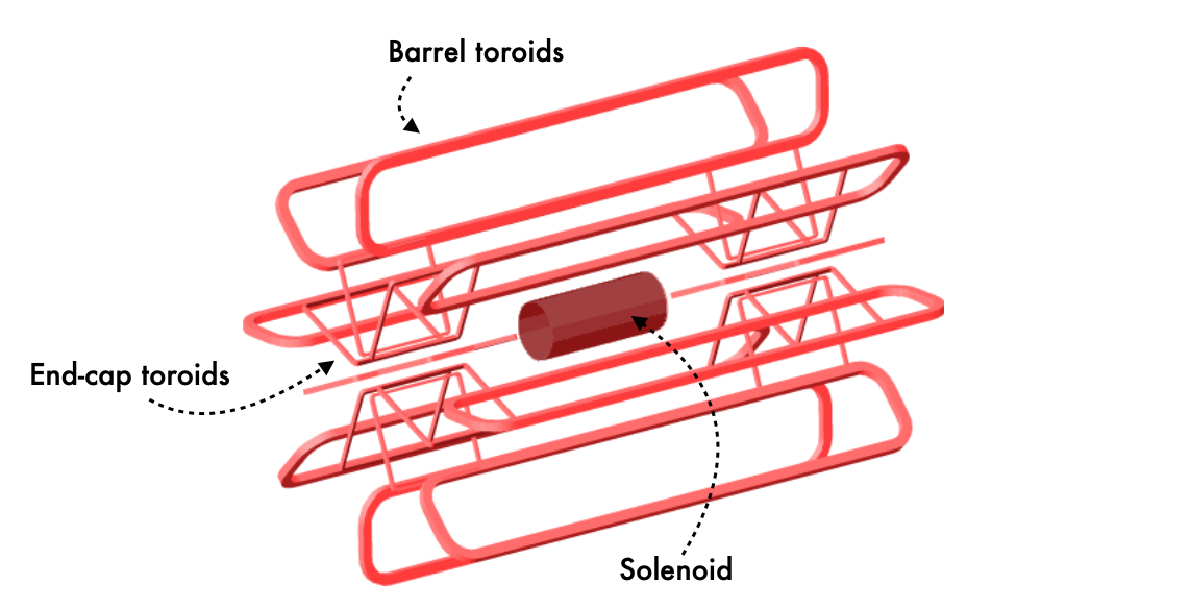
\includegraphics[width=0.85\textwidth]{figures/Chap3/Rizzi-Fig3-10-1.pdf}}
\caption{Layout of the \gls{atlas} magnet system. Figure adapted from Ref. \cite{Goodson}.}
\label{fig:atlas:magnet}
\end{figure}

As discussed in Section \ref{sec:dec:tracking}, the magnetic field configurations that are more suitable for a detector with cylindrical symmetry are solenoidal and toroidal. The bending of the charged particles in the \gls{atlas} \gls{id} is caused by an axial 2 T solenoidal field, provided by the central solenoid \cite{YAMAMOTO200853}. This magnet is 5.8 m long, has an inner diameter of 2.46 m and an outer diameter of 2.56. The wounded coil is made of an Al-stabilized NbTi conductor, and is powered with a 7.73 kA current. 


In the muon system, a solenoid would be disadvantageous in the measurement of forward muons, since the resultant magnetic field would not be perpendicular to the trajectory of those particles. The usage of a toroid to provide the outer magnetic field solves this problem. 
The choice of the “open air” toroid configuration allows a good muon
reconstruction performance without relying on the \gls{id}. 
The toroids allow to efficiently generate the magnetic field over a large volume with a reduced amount
of material. This minimizes the amount of multiple scattering, which represents one
of the factors limiting the muon momentum resolution.
The main drawback of the usage of a toroid is that, in order to obtain the same strength of magnetic field, a toroid needs more current than a solenoid (20.5 kA for 4 T).
The \gls{atlas} toroid system is divided into two subsystems, to allow for an easier design, 
as well as to provide access to the core part of the detector.
The barrel toroid \cite{ATLAS:1997ac} provides a peak field of 3.9 T in the cylindrical shell between the calorimeters and the end of the muon spectrometer, and consists of eight coils contained in individual vacuum vessels.  
The end-cap toroids \cite{ATLAS:1997ab} provide the magnetic field necessary to bend the muons in the end-cap region of the spectrometer, and each of them consists of eight coils building a single cold mass, originating a peak field of 4.1 T. 



\subsection{Inner detector}
\label{sec:atlas:id}

The main purposes of the \gls{atlas} \gls{id} \cite{ATLAS:1997ag,ATLAS:1997af} are to provide a good momentum resolution of the charged particles produced in the collisions and to allow the determination of secondary vertices. The dimensions of the \gls{id} are determined on one side by the 
radius of the beam pipe and on the other side by the beginning of the \gls{ecal}. The total length is 5.4 m, which provides a coverage up to $|\eta|<$2.5.
The \gls{id} is divided into a barrel, whose schema is shown in Figure \ref{fig:atlas:id}, and two end-cap regions, covering respectively the pseudorapidity regions $|\eta|<1.2$ and $1.2<|\eta|<2.5$. In both, a mixture of gaseous and silicon detectors is used to maximize the performance and reduce the costs. The three components of the \gls{id} are the pixel detector, the semi-conductor tracker, and the transition radiation tracker, discussed in the following paragraphs.

\begin{figure}[ht]
\centering
\subfigure{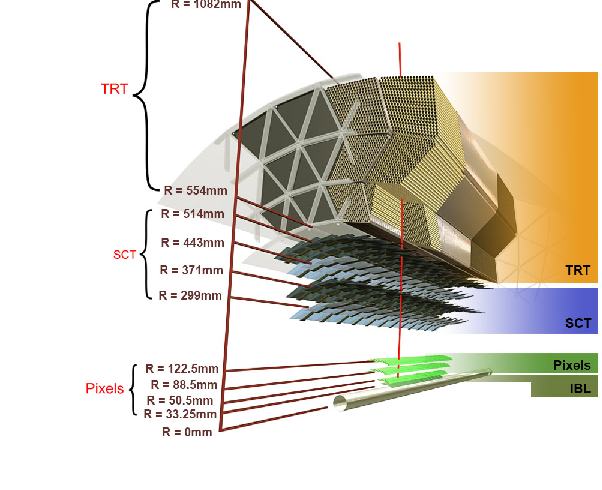
\includegraphics[width=0.65\textwidth]{figures/Chap3/Rizzi-Fig3-11-1.pdf}}
\caption{Layout of the \gls{atlas} \gls{id}. Figure from Ref. \cite{Potamianos:2016ptf}.}
\label{fig:atlas:id}
\end{figure}


\subsubsection*{Pixel detector}
\label{sec:atlas:pixel}
The innermost layer of the \gls{id} is the pixel detector \cite{Aad:2008zz}, divided into barrel and end-cap regions. 
During the Long Shutdown after the \gls{lhc} Run 1, the \gls{id} was subject to important upgrades \cite{Potamianos:2016ptf}. 
The main one is the addition of a fourth pixel layer in the barrel, in addition to the three already existing ones, 
the \gls{ibl} \cite{Capeans:1291633}, that is positioned 3.33 cm away from the \gls{ip}. 
In order to locate a detector so close to the \gls{ip}, the beam pipe had to be replaced with a thinner one. 
The \gls{ibl} is 72.4 cm long along the $z$-direction, and consists of 14 staves that provide full coverage in azimuthal angle. Each stave contains 20 modules, 12 with planar silicon sensors and eight with 3D pixel sensors \cite{1748-0221-7-11-P11010}, and each module has 144$\times$328 pixels with an area of 50$\times$250 $\mu$m$^2$ and a depth of 200 $\mu$m and 230 $\mu$m for the planar and 3D sensors respectively, 
for a total of over 12 million pixels in the entire \gls{ibl}. The size of the pixels leads to a resolution of 40 and 8 $\mu$m respectively in the longitudinal and transverse direction. 
The three outer pixel layers are located at 5.05, 8.85 and 12.5 cm from the \gls{ip}. 
Each module contains 80 pixels with an area of 50$\times$400 $\mu$m$^2$ and a depth of 250 $\mu$m, leading to a spatial resolution of 115 and 10 $\mu$m respectively in the longitudinal and transverse direction. 
The two end caps, on the two sides of the detector, consist of three wheels each, with a radius of 34 cm and located at 49.5, 58.8 and 65.0 cm from the \gls{ip}. 
To ensure a good performance, the pixel detectors need to be kept at a low and stable temperature, 
between -15$^{\circ}$ C and 5$^{\circ}$ C for the \gls{ibl}, and between -15$^{\circ}$ C and -10$^{\circ}$ C for the other layers.

\subsubsection*{Semi-conductor tracker}
The \gls{atlas} \gls{sct} is composed by 4088 silicon micro-strip modules with binary readout mounted on carbon fibre composite structures, and is organized in four cylinders in the barrel and nine disks in each of the forward regions \cite{Jackson:sct}. The cylinders have  radii of 30.0, 37.3, 44.7 and 52.0 cm and provide a coverage for $|\eta|<1.1-1.4$, while the disks cover the region with $1.1-1.4<|\eta|<2.5$. 
Out of the 4088 \gls{sct} modules, 2112 modules are in the barrel, 
and contain single-sided p-in-n silicon strips, with a pitch of 80 $\mu$m. 
In each module, the strip sensors are positioned back to back with an angle of 40 mrad, to be able to access information on the $z$-coordinate as well. The end-cap modules use strips with width between 56.9 and 94.2 $\mu$m. 
These choices lead to a spatial resolution of 580 $\mu$m in the longitudinal direction and 17 $\mu$m in the transverse one.
Also the \gls{sct} components need to be kept at a low temperature, between -15$^{\circ}$ C and -5$^{\circ}$ C.

\subsubsection*{Transition radiation tracker}

The \gls{trt} is the outermost layer of the \gls{id}. In the barrel it consists of 52544 straw tubes with a length of 1.5 m disposed parallel to the beam direction, while each end-cap contains 122880 straw tubes 0.4 m long disposed perpendicularly to the beam axis. Each tube is 4 mm in diameter, and has in the inside gold plated tungsten wire as anode with a diameter of 31 $\mu$m. The tubes are filled with a mixture of 70\% Xe, 27\% CO$_2$ and 3\% O$_2$; due to a gas leakage, in 2016 part of the \gls{trt} tubes have been filled with a cheaper mixture of 80\% Ar and 20\% CO$_2$. The \gls{trt} has a pseudorapidity coverage up to $|\eta|<2$ and it provides tracking information only in the (r-$\phi$) plane, with a resolution of 130 $\mu$m.


\subsection{Calorimeters}
\label{sec:atlas:calo}

The \gls{atlas} calorimeter system is located outside the \gls{id} and the magnetic field of the solenoid, as shown in Figure \ref{fig:atlas:calo}. The \gls{ecal} is closer to the \gls{ip}, while the \gls{hcal} is on the outside; both systems have a barrel and an end-cap section. 
The combined thickness of the calorimeter system is about 11 interaction lengths to ensure the longitudinal containment of energetic jets, 
as well as a good reconstruction of the energy imbalance in the event, which is a measure of the energy carried away by neutral weakly-interacting particles. The total pseudorapidity coverage is up to $|\eta|<4.9$. 

\begin{figure}[ht]
\centering
\subfigure{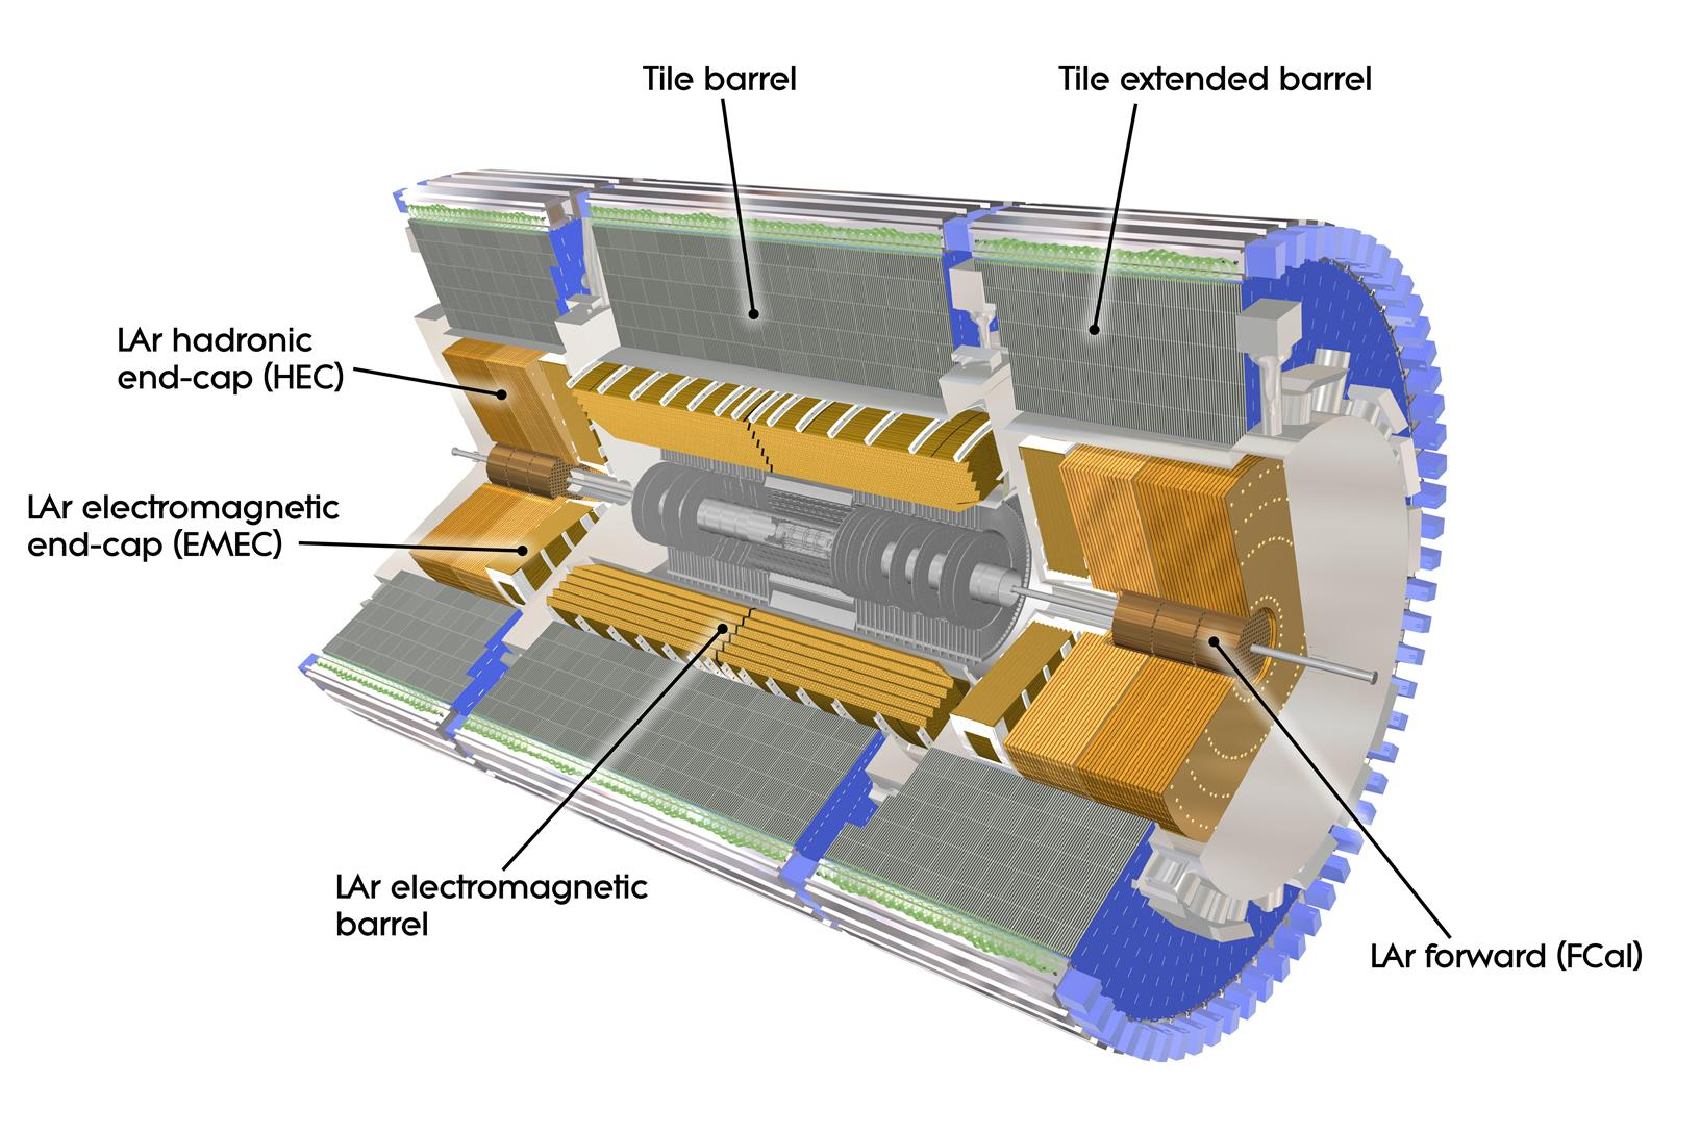
\includegraphics[width=0.75\textwidth]{figures/Chap3/Rizzi-Fig3-12-1.pdf}}
\caption{Layout of the \gls{atlas} calorimeter system. Figure from Ref. \cite{atlas:atlas}.}
\label{fig:atlas:calo}
\end{figure}

Table \ref{tab:atlas:cal:reso} summarizes the energy resolution of the different subsystems. As expected from the discussion in Section \ref{sec:dec:calo}, the resolution is better for electromagnetic showers than for the hadronic ones. For example, a 1 GeV particle detected in the \gls{ecal} has an energy resolution of about 19\%, while 50\% (100\%) if detected in the \gls{hcal} barrel (end-caps). On the other hand, a 1 TeV particle has an energy resolution of 0.7\% in the \gls{ecal} and 3\% (10\%) in  \gls{hcal} barrel (end-caps), and in this case the resolution is dominated by the constant term, 
related to instrumental effects and to the different response of the detectors to electromagnetic and hadronic showers. 

\begin{table}[ht]
\begin{center}
\begin{tabular}{c c }
\hline
Component & $\sigma_E / E$ \\
\hline 
\hline
\gls{ecal} & 0.1$/\sqrt{E[GeV]}$ $\bigoplus$ 0.17$/E$ $\bigoplus$ 0.007 \\ % chiara: cite LAr TDR
\hline
\gls{hcal} barrel & 0.5$/\sqrt{E[GeV]}$ $\bigoplus$ 0.03 \\
\hline
\gls{hcal} end caps & 1$/\sqrt{E[GeV]}$ $\bigoplus$ 0.1 \\
\hline
\end{tabular}
\end{center}
\caption{Energy resolution of the \gls{atlas} calorimeters.}
\label{tab:atlas:cal:reso}
\end{table}

\begin{figure}[ht]
\centering
\subfigure[]{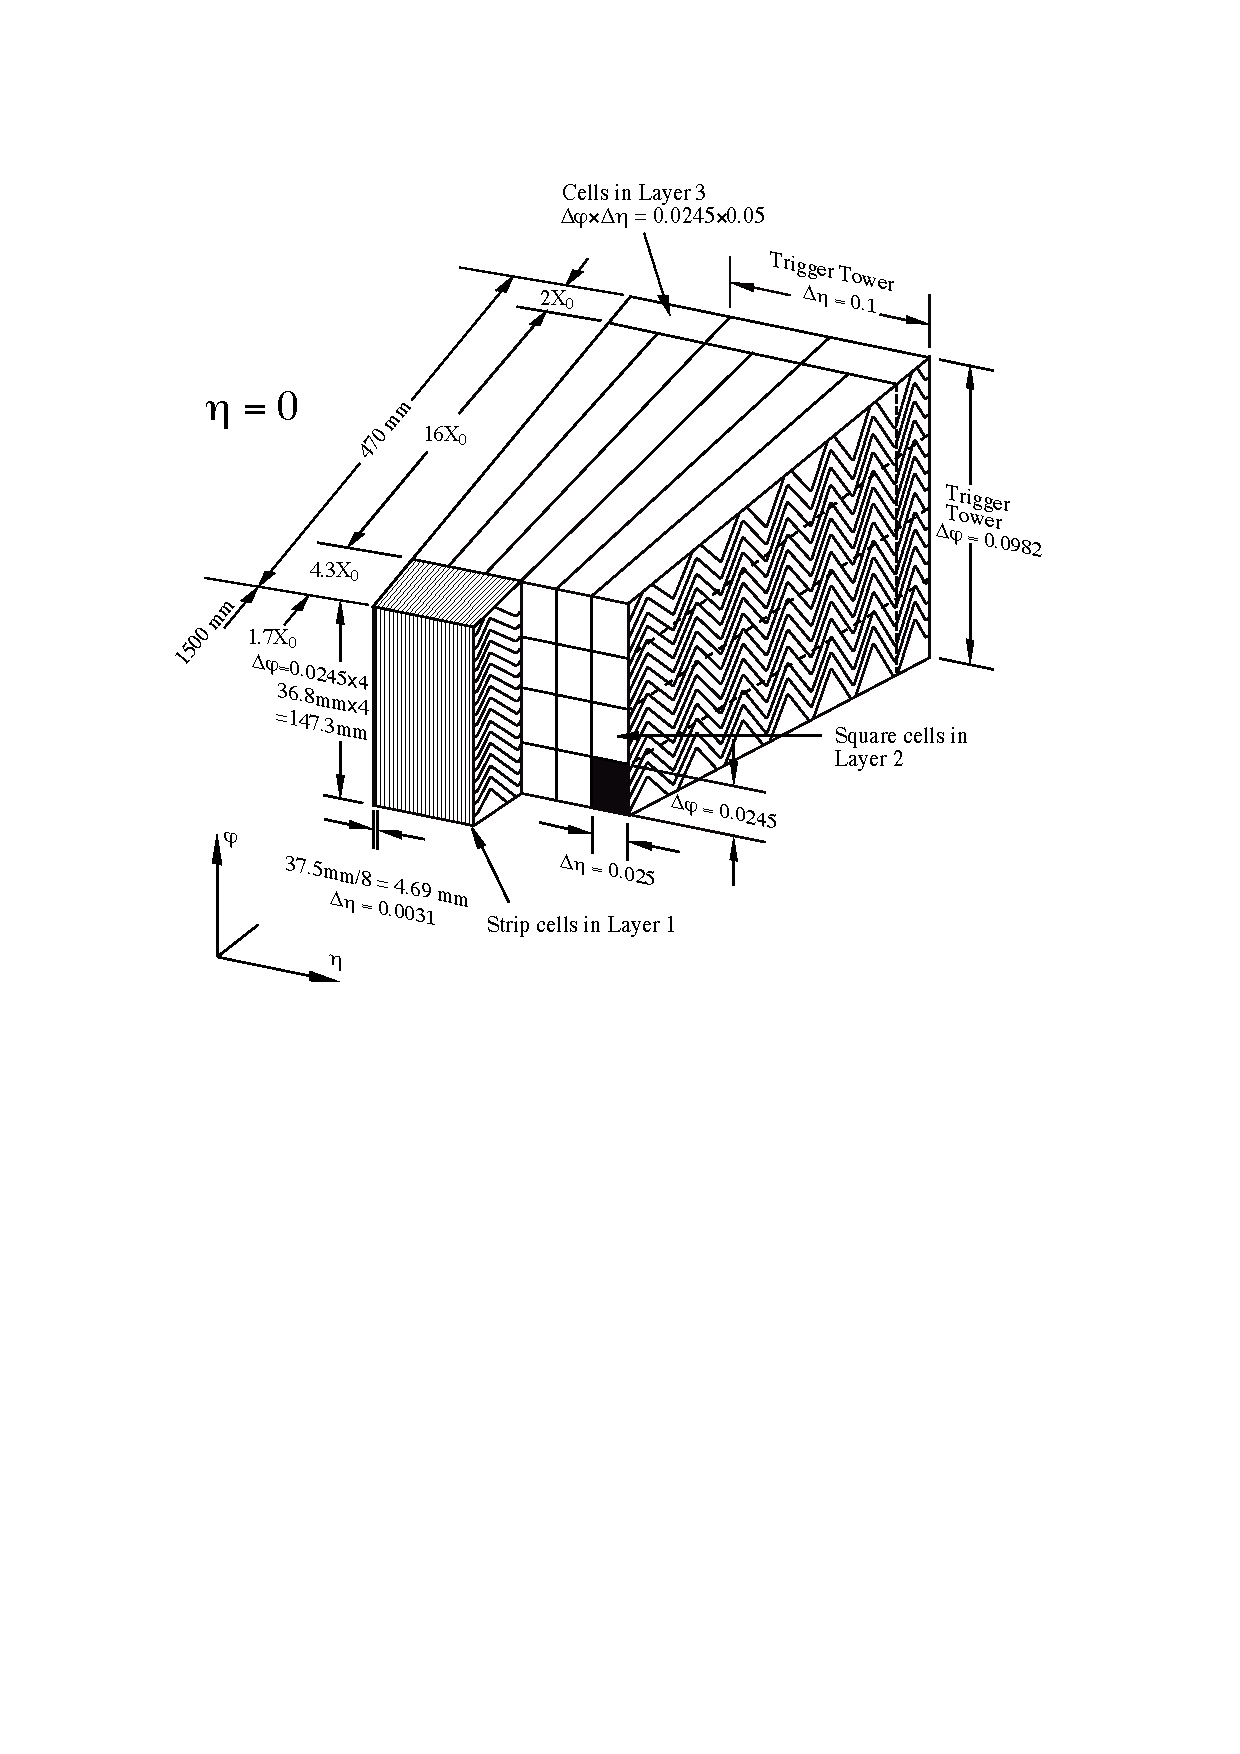
\includegraphics[width=0.495\textwidth]{figures/Chap3/Rizzi-Fig3-13-1.pdf}}
\subfigure[]{\includegraphics[width=0.495\textwidth]{figures/Chap3/Rizzi-Fig3-13-2.pdf}}
\caption{(a) Schema of a barrel module of the \gls{atlas} \gls{ecal}. Figure from Ref. \cite{atlas:atlas}. (b) Accordion shape of the metal plates of the \gls{ecal}.}
\label{fig:atlas:lar}
\end{figure}

\subsubsection*{Electromagnetic calorimeter}

The \gls{ecal} is a sampling calorimeter with \gls{lar} as active material and lead plates as absorber, both in the barrel and in the end caps. The lead plates have a characteristic accordion shape and, in the barrel, are oriented in the radial direction. Before the \gls{ecal}, a presampler provides the information necessary to reconstruct the amount of energy lost in the passive material of the solenoid. The design of a \gls{lar} barrel module is shown in Figure \ref{fig:atlas:lar}(a), where it is possible to see the segmentation in three layers with decreasing granularity: the first layer is finely segmented in pseudorapidity, with strips of $\Delta\eta \times \Delta\phi = 0.0031 \times 0.098$; the second layer has towers of $\Delta\eta \times \Delta\phi =  0.025 \times 0.025$ to measure the clusters, while the third layer has wider towers of $\Delta\eta \times \Delta\phi =  0.05 \times 0.0245$ to provide an estimate of the energy leaking outside the \gls{ecal}. The \gls{lar} barrel offers pseudorapidity coverage up to $|\eta|<$1.475, and the thickness of the detector varies from 22 $X_0$ at $\eta=0$ to 33 $X_0$ at $|\eta|=1.3$. 
Each of the two end-cap regions consists of two coaxial wheels, of eight modules each, that cover the region $1.375<|\eta|<3.2$, with a thickness varying between 26 and 36 $X_0$ for the inner wheel and between 24 and 38 $X_0$ for the outer wheel. The end-cap modules are divided into two layers, again with decreasing granularity.


\subsubsection*{Hadronic calorimeter}

The hadronic calorimeter is composed of three subsystems with different technologies: the \gls{tilecal} \cite{TileTDR} is a sampling calorimeter with plastic scintillator as active material and steel as absorber, the hadronic end-cap calorimeter (HEC) uses copper as absorber and liquid argon as scintillator, while the forward calorimeter (FCal) also uses liquid argon in the active layer but has tungsten rods embedded in a copper matrix as absorber. The choice of the materials is driven by the need to have detectors more resistant to radiation in the forward region, where the flux of particles is larger. 

\gls{tilecal} covers the pseudorapidity region with $|\eta|<1.7$, and is divided into a central \gls{lb}, 5.8 m long, and two \glspl{eb}, 2.6 m long; the \gls{tilecal} inner radius is 2.28 m, and the outer radius 4.25 m. Each barrel is divided in 64 modules, disposed on the $\phi$ direction and each having the size of 0.1 radians. Each module is further segmented radially into three layers with thicknesses of about 1.5, 4.1 and 1.8 $\lambda_I$ in the \gls{lb} and 1.5, 2.6 and 3.3 $\lambda_I$ in the \gls{eb}; a schematic of one module is shown in Figure \ref{fig:atlas:tile}(a). Ionizing particles passing through the plastic scintillator (polystyrene) produce ultra-violet light, which is then collected at the two edges of each tile and converted to the longer wavelength of visible light by wavelength-shifting fibers. The fibers, with a diameter of 1 mm each, transmit the light to the readout \glspl{pmt} located in the grinder.

\begin{figure}[ht]
\centering
\subfigure[]{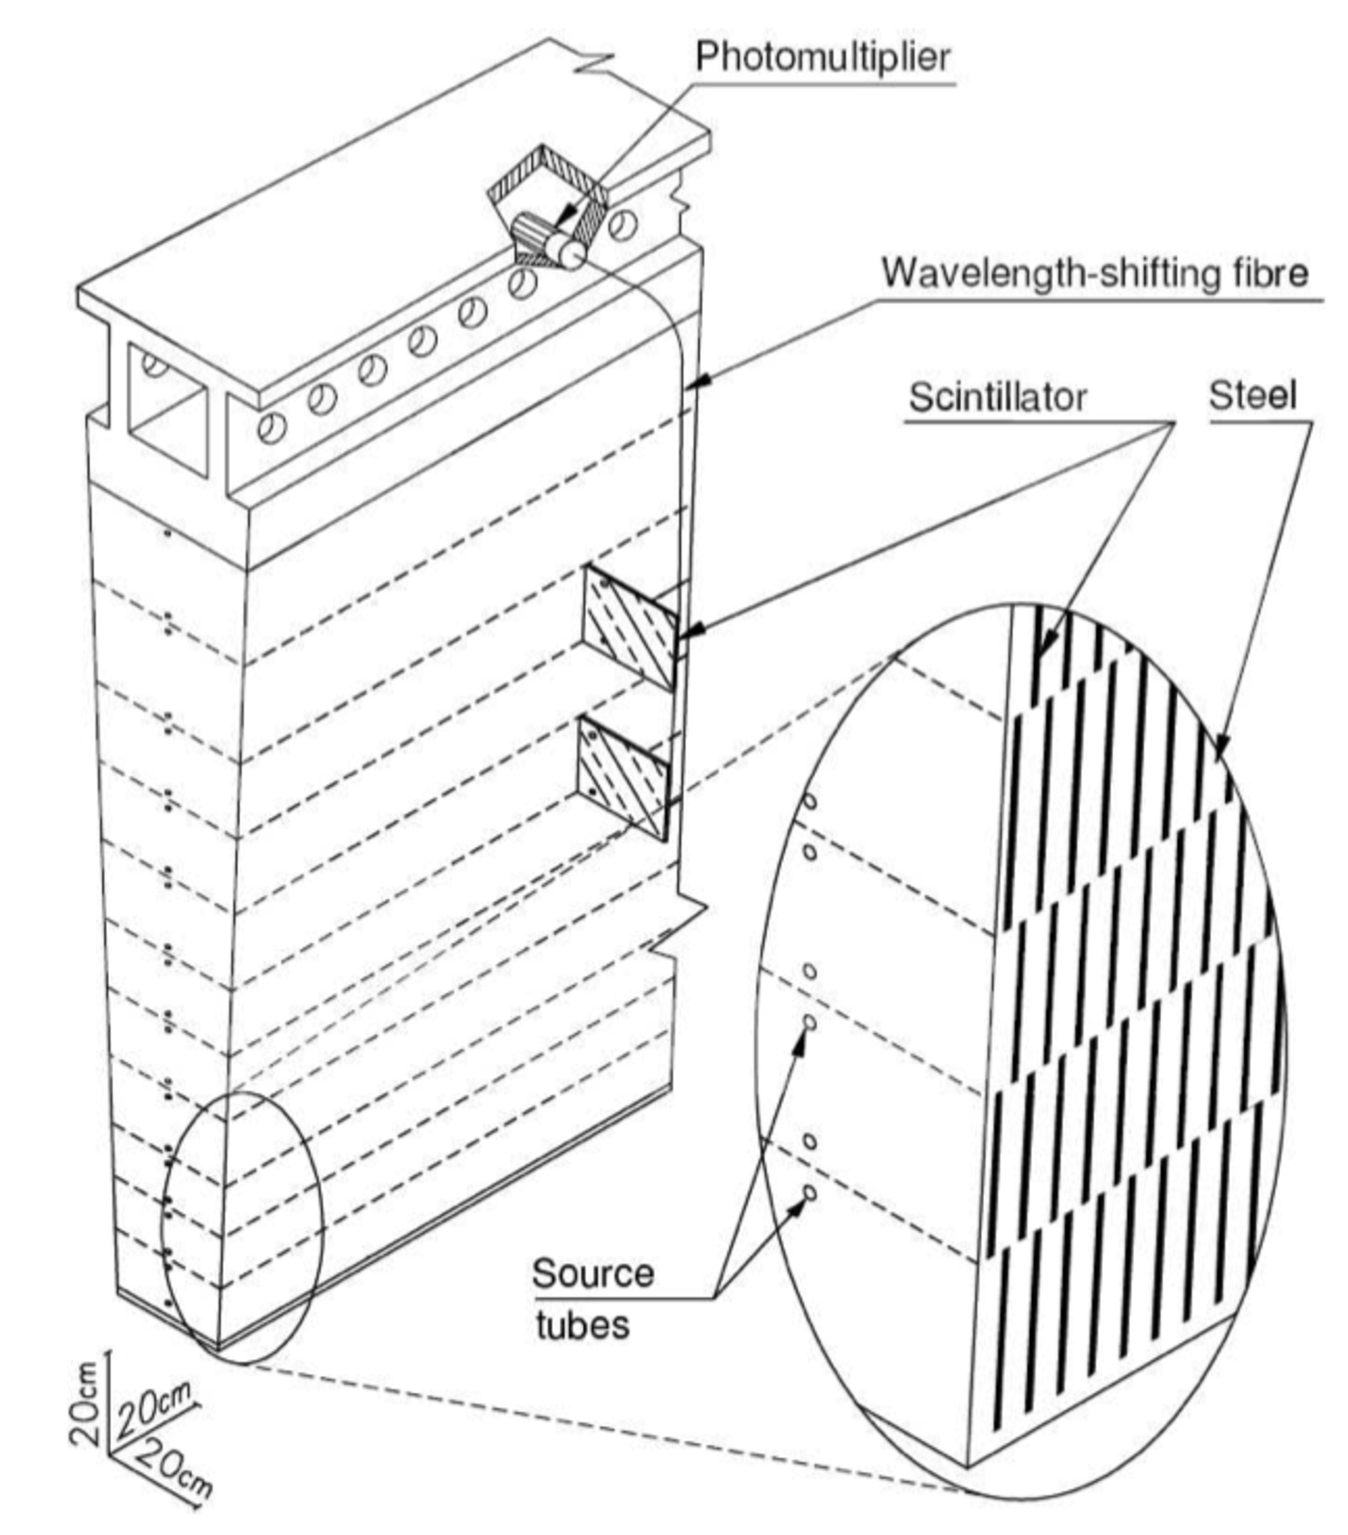
\includegraphics[width=0.4\textwidth]{figures/Chap3/Rizzi-Fig3-14-1.pdf}}
\subfigure[]{\includegraphics[width=0.59\textwidth]{figures/Chap3/Rizzi-Fig3-14-2.pdf}}
\caption{(a) Schematic representation of a \gls{tilecal} module and its interface with the optical readout. Figure from Ref. \cite{atlas:atlas}. (b) \gls{tilecal} modules before the installation.}
\label{fig:atlas:tile}
\end{figure}

An approximately projective geometry, shown in Figure \ref{fig:atlas:tile_cells}, is provided by the grouping of the readout fibers into the \glspl{pmt}: this defines a cell structure, and each cell has dimension $\Delta\eta \times \Delta\phi = $ 0.1 $\times$ 0.1 in the first two layers and $\Delta\eta \times \Delta\phi = $ 0.2 $\times$ 0.1 in the third layer. Special cells cover the gap region between the \gls{lb} and the \gls{eb}: the gap scintillators in the pseudorapidity region $1.0<|\eta|<1.2$ and the crack scintillators in the region $1.2<|\eta|<1.6$, in front of the \gls{lar} end caps.

\begin{figure}[ht]
\centering
\subfigure{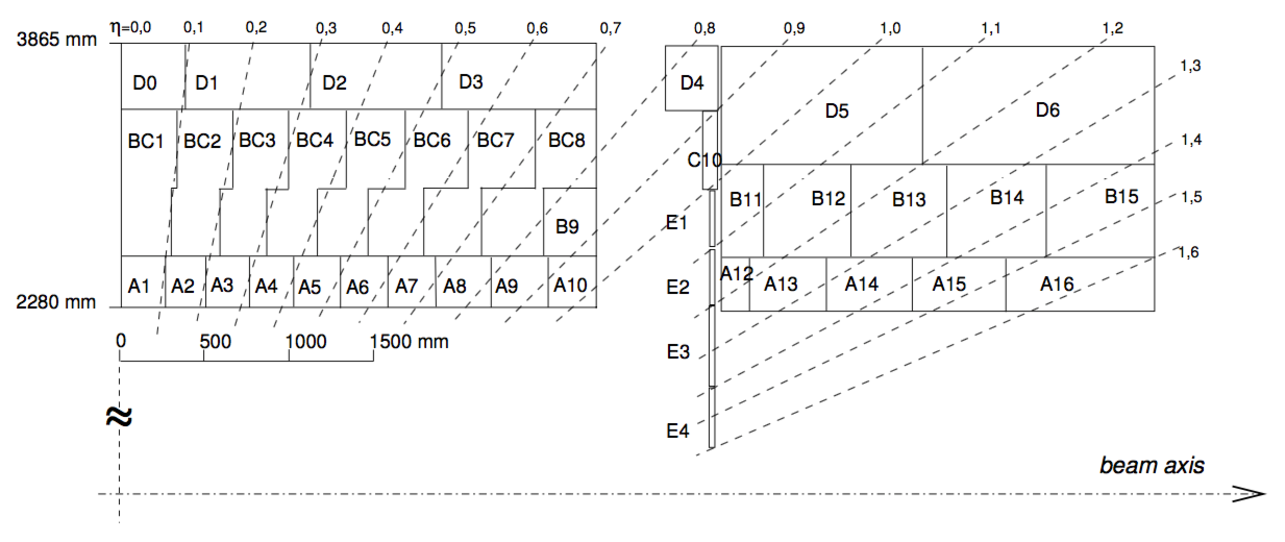
\includegraphics[width=1.0\textwidth]{figures/Chap3/Rizzi-Fig3-15-1.pdf}}
\caption{Layout of the projective geometry of the \gls{tilecal} cells. Figure from Ref. \cite{atlas:atlas}.}
\label{fig:atlas:tile_cells}
\end{figure}

The HEC shares the same cryogenic system as the \gls{ecal} end caps, and covers the region with $1.5<|\eta|<3.2$. Liquid argon is more resistant to radiation than the plastic scintillator used in \gls{tilecal}, and is therefore the preferred choice in the end-cap region. Each side of the HEC consists of two wheels with outer radius of 2.03 m, and each wheel is composed by 32 identical modules. The electromagnetic signal produced in the \gls{lar} is collected by cathodes on the plates. 

The FCal provides coverage in the forward region with $3.1<|\eta|<4.9$. The FCal modules are located at high pseudorapidity, at a distance of 4.7 m along the $z$-axis from the \gls{ip}.


\subsection{Muon spectrometer}

The \gls{ms} \cite{ATLAS:1997ad}, shown in Figure \ref{fig:atlas:muon}, is the outer layer of the \gls{atlas} detector, and is located in the magnetic field produced by the 4 T toroidal magnets described in Section \ref{sec:atlas:magnets}. It is designed to provide a \pt measurement with a relative uncertainty of 3\% for muons of intermediate \pt, and to maintain a low uncertainty also at higher \pt (about 10\% for muons with \pt of 1 TeV). It consists of four different muon chambers, two dedicated to the precise measurement of the muon tracks traversing the detector, 
and two providing fast event selection for the trigger system. 

\begin{figure}[ht]
\centering
\subfigure{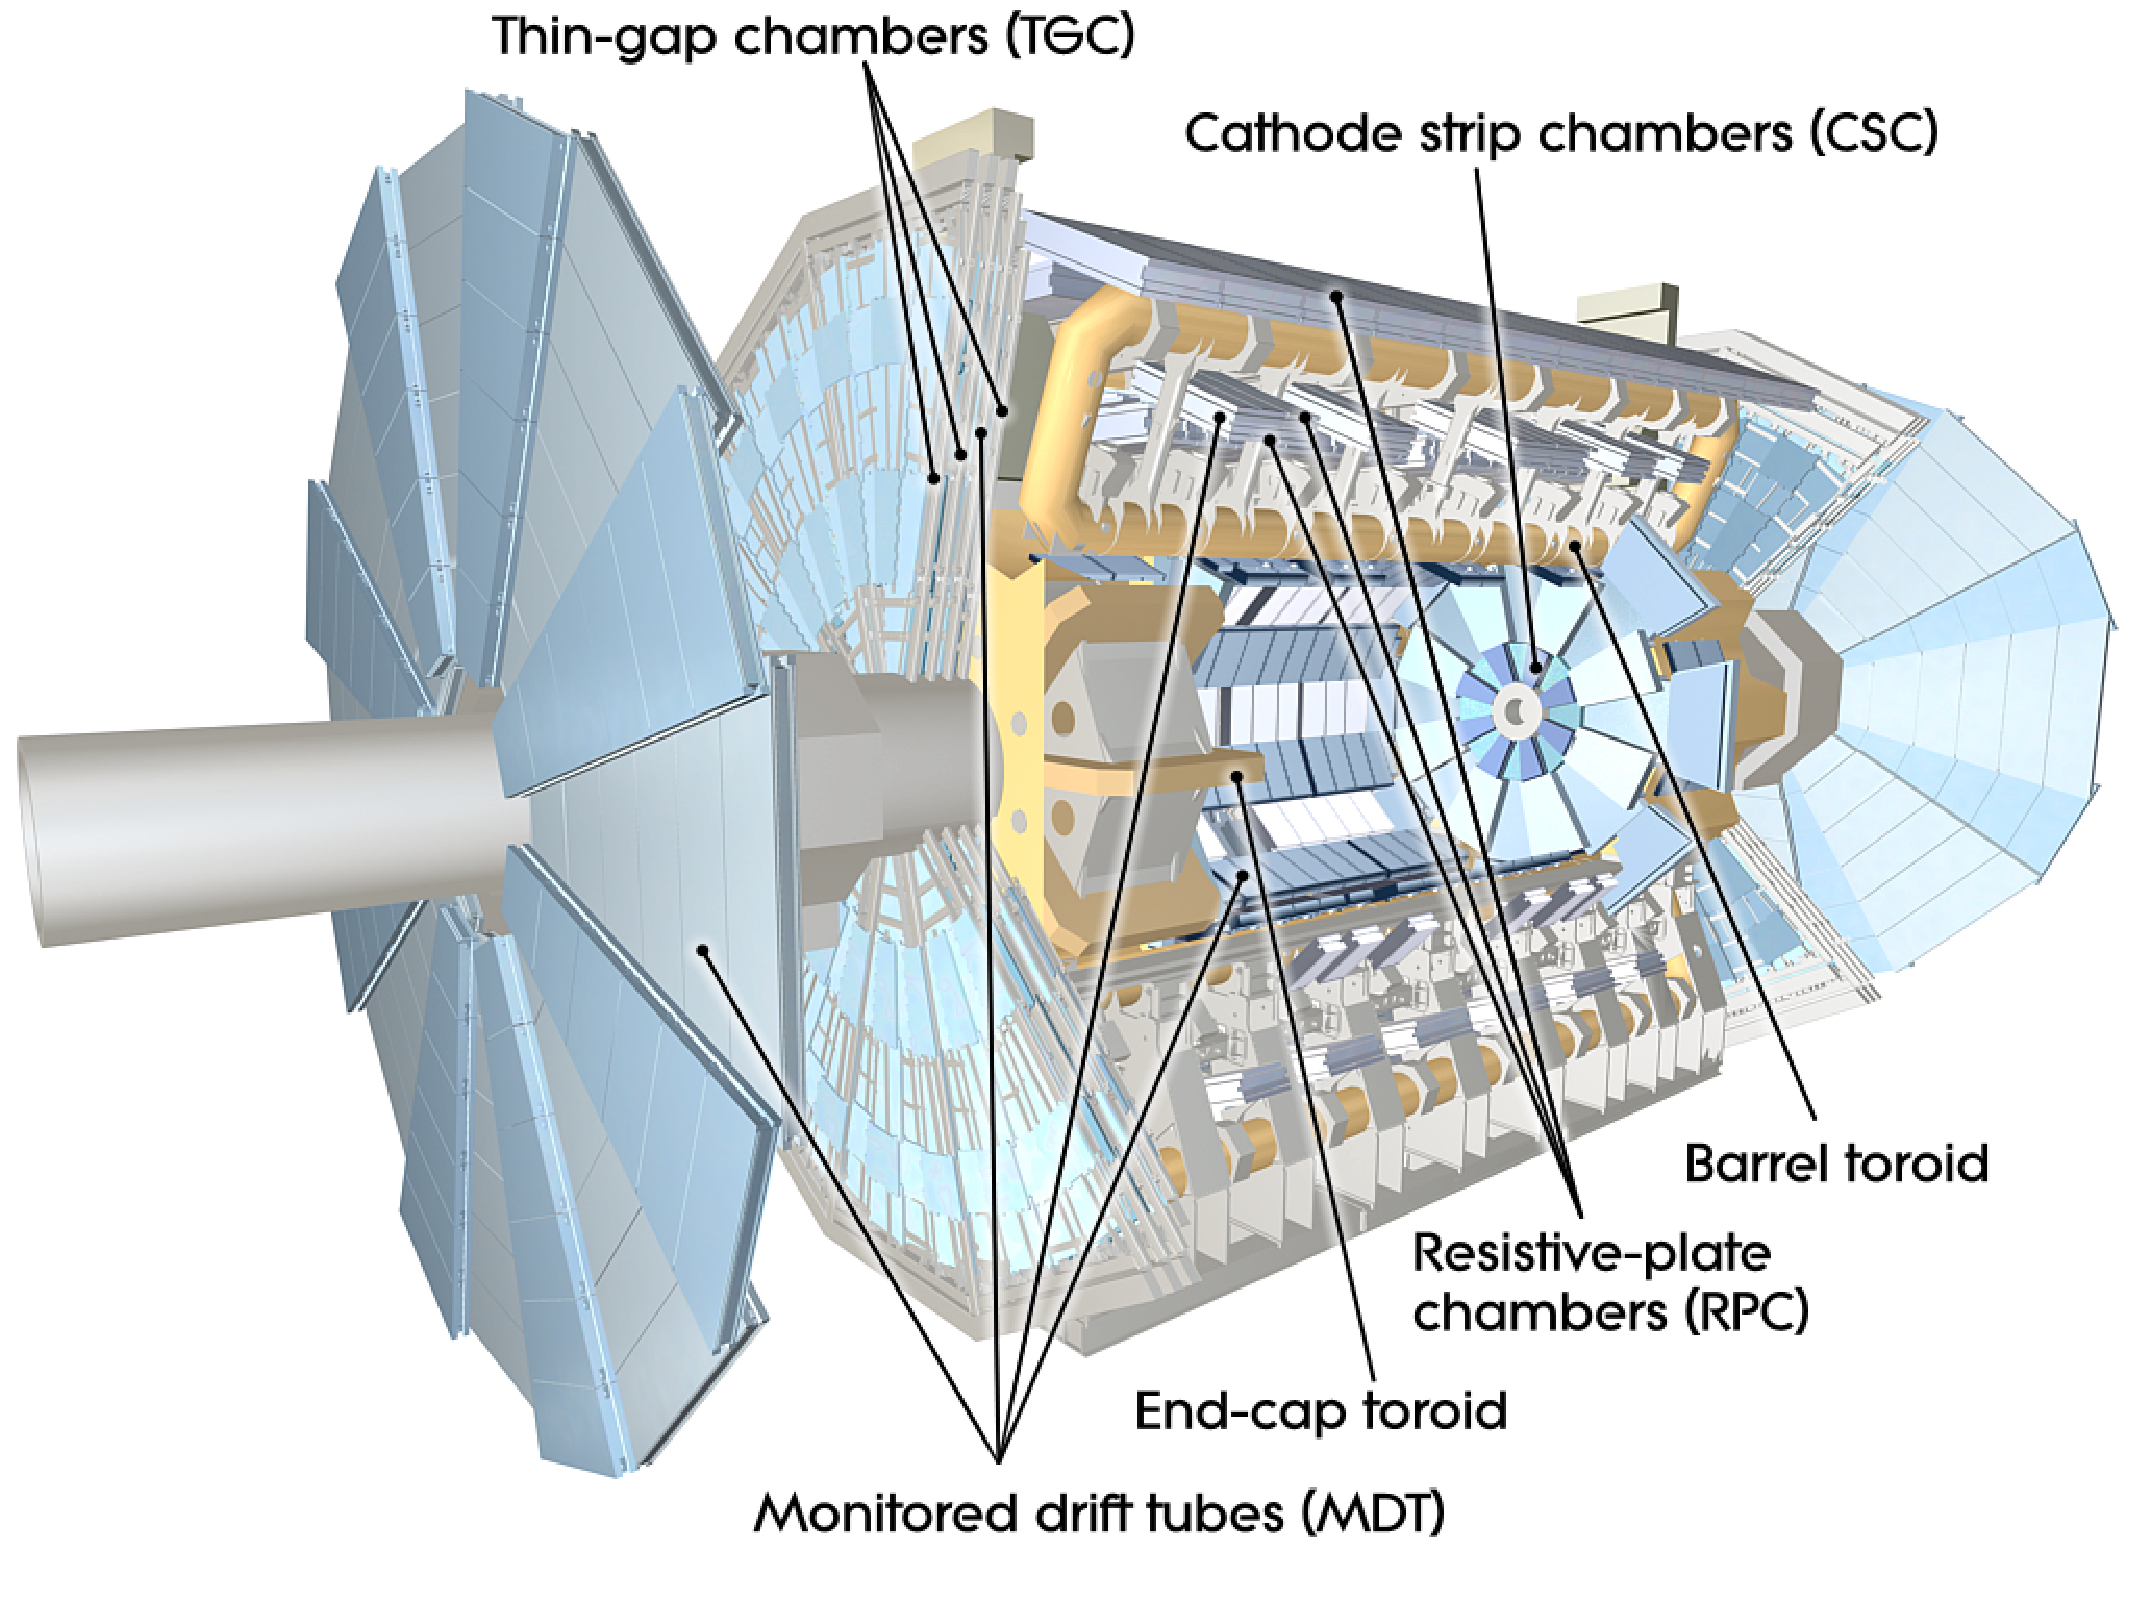
\includegraphics[width=0.65\textwidth]{figures/Chap3/Rizzi-Fig3-16-1.pdf}}
\caption{Layout of the \gls{atlas} muon system. Figure from Ref. \cite{atlas:atlas}.}
\label{fig:atlas:muon}
\end{figure}

The two systems dedicated to precision measurement are the \gls{mdt} and the \gls{csc}, both present in barrel and end caps. The \glspl{mdt} are proportional drift chambers covering the region $|\eta|<2.7$; they are made of aluminium tubes with a diameter of 30 mm and a length between 700 and 6300 mm, and a cathode wire made of an alloy of tungsten (97\%) and rhenium (3\%). The filling gas is a mixture of Ar, N$_2$, and CH$_4$ with percentages respectively of 91\%, 4\% and 5\%. The \glspl{csc} are multi-wire proportional chambers that cover the region with $2.0<|\eta|<2.7$, where the shorter drift time of this detector (30 ns compared to the 480 ns of the \glspl{mdt}) allows to better cope with the increase in particle flux in the forward region. The anode wires in the \glspl{csc} are made of the same tungsten-rhenium alloy of the \glspl{mdt} and have a 2.54 mm pitch, which is the same distance separating them from the copper cathode strips, creating a symmetric cell. The gas inside the chamber is a mixture of 30\% Ar, 50\% CO$_2$, and 20\% CF$_4$. The spatial resolution is 40 $\mu$m in the bending plane and 5 mm in the perpendicular plane.

The muon trigger system needs to be able to identify events with energetic muons in a timescale compatible with assigning them to the correct bunch crossing, that are spaced by 25 ns. The two trigger chambers are the \gls{rpc} and the \gls{tgc}. The \glspl{rpc} are arranged in three layers in the barrel region, outside the outermost \gls{mdt} layer. Each narrow chamber consists of two parallel resistive bakelite plates and is filled with a mixture of 94.7\% C$_2$H$_2$F$_4$, 5\% Iso-C$_4$H$_{10}$, and 0.3\% SF$_6$. The signal is read out by metal plates through capacitive coupling, providing a time resolution of 1.5 ns, while the space resolution is about 1 cm. The \gls{rpc} also provides the $\phi$ coordinate for the track, which is not measured by the \glspl{mdt}. The \glspl{tgc} are multi-wire proportional chambers located in the end caps, filled with a mixture of 55\% CO$_2$ and 45\% n-C$_5$H$_{12}$. Contrarily to the \glspl{csc}, the \glspl{tgc} are characterized by a distance between the cathode and the anode shorter than the anode pitch. The pseudorapidity coverage is $1.05<|\eta|<2.7$ for tracking and $1.05<|\eta|<2.4$ for triggering; the time response is similar to that of the \glspl{rpc}, while the spatial resolution is better: between 2 and 7 mm. 

\subsection{Luminosity measurement}
\label{sec:lumimeas}

An accurate determination of the luminosity is important both for \gls{sm} measurements, where the luminosity uncertainty can dominate in some cases, and for \gls{bsm} searches, where a precise background estimate is a key ingredient to be sensitive to a signal. In the \gls{atlas} detector the luminosity measurement is performed with redundancy by multiple luminometers that use different technologies and algorithms, to allow a better determination of the final number and to assign systematic uncertainties. The instantaneous luminosity in Equation \ref{eq:cern:lumi} can also be expressed following the conventions in Ref. \cite{Aaboud:2016hhf} as product of the number of bunch crossings $N_b$ and the average luminosity per bunch cross ${<}\mathcal{L}_b{>}$:
\begin{equation}
\mathcal{L} = N_b {<}\mathcal{L}_b{>} = N_b \frac{f {<}\mu{>}}{\sigma_{\mathrm{inel}} } \; .
\label{eq:atlas:lumi}
\end{equation}

With respect to the nomenclature of Equation \ref{eq:cern:lumi}, ${<}\mu{>}$ is the average pileup per bunch crossing and $\sigma_{\mathrm{inel}}$ the inelastic \gls{pp} cross-section. Because of the finite acceptance and efficiency of the detector, what is measured is:
\begin{equation}
\mathcal{L}_b = \frac{f {<}\mu_\mathrm{vis}{>}}{\sigma_{\mathrm{vis}} } \; , \nonumber
\end{equation}

\noindent where ${<}\mu_\mathrm{vis}{>}$ and $\sigma_{\mathrm{vis}}$ are the product of the corresponding quantities in Equation \ref{eq:atlas:lumi} and the acceptance and efficiency of the detector. Out of these two quantities, ${<}\mu_\mathrm{vis}{>}$ is directly measurable during the collisions, while $\sigma_{\mathrm{vis}}$ is determined with the \gls{vdm} method \cite{vanderMeer:296752}, carried out in the dedicated \gls{vdm} runs. These are special runs with low bunch intensity and number of bunches, where a variation (scan) of the overlap of the two beams in the $x$- and $y$-direction is performed; the beam parameters and the peak of visible interaction rate per bunch crossing during the scan can be used to determine the visible cross-section and therefore calibrate each subsystem. 

We can express the luminosity per bunch cross as:
\begin{equation}
\mathcal{L}_b = n_1 n_2 f \int \rho_1(x,y) \rho_2(x,y) \, dx \, dy \; ,
\label{eq:lumi_vdm1}
\end{equation}

\noindent where $\rho_1(x,y)$ and $\rho_2(x,y)$ are the particle densities in the two colliding bunches at the \gls{ip}. 
Under the assumption that these densities can be factorized into the horizontal and vertical components, we can write Equation \ref{eq:lumi_vdm1} as:
\begin{equation}
\mathcal{L}_b = n_1 n_2 f  \Omega_x(\rho_1(x), \rho_2(x)) \Omega_y(\rho_1(y), \rho_2(y))  \; , \nonumber
\label{eq:lumi_vdm2}
\end{equation}

\noindent where $\Omega_{x/y}$ defines the beam overlap in the $x$/$y$ direction.

The relevant quantity in physics analyses is the integrated luminosity over a defined period of time. The basic time unit over which the integrated luminosity is computed and stored is the \gls{lub}, whose duration is defined by the \gls{atlas} trigger system and is typically about one minute. The data contained in each \gls{lub} is collected with the same detector conditions, and the integrated luminosity is computed as the average instantaneous luminosity multiplied by the \gls{lub} time duration.

\gls{atlas} has two primary specifically-designed luminometers, LUCID-2 (LUminosity measurements using Cherenkov Integrating Detector) and \gls{bcm}, whose results are compared with the ones obtained by other \gls{atlas} subsystems that measure luminosity through quantities that are sensitive to it, such as the number of tracks or the flow of particles.

\subsubsection*{Bunch-by-bunch luminometers}

The two dedicated luminometers are able to provide information for individual bunch crossings, each labeled by a \gls{bcid}.

\gls{bcm} consists of four $8 \times 8$ mm$^2$ diamond sensors, located at $z= \pm 184$ m from the \gls{ip} and disposed in a cross shape around the beam pipe, at $|\eta| = 4.2$. Beside luminosity measurements, \gls{bcm} also contributes to recognize beam losses so that the beam can be dumped before damaging the silicon detectors. 

LUCID is located 17 m from the \gls{ip}, at $5.6 < |\eta| < 6.0$, and consists on each side of 16 Cherenkov detectors built by aluminum tubes with a diameter of 10 mm. Cherenkov radiation is produced in the passage of particles through the quartz windows of the \glspl{pmt}. A signal over threshold produces a hit for that bunch crossing.

%\begin{figure}[ht]
%\centering
%\subfigure{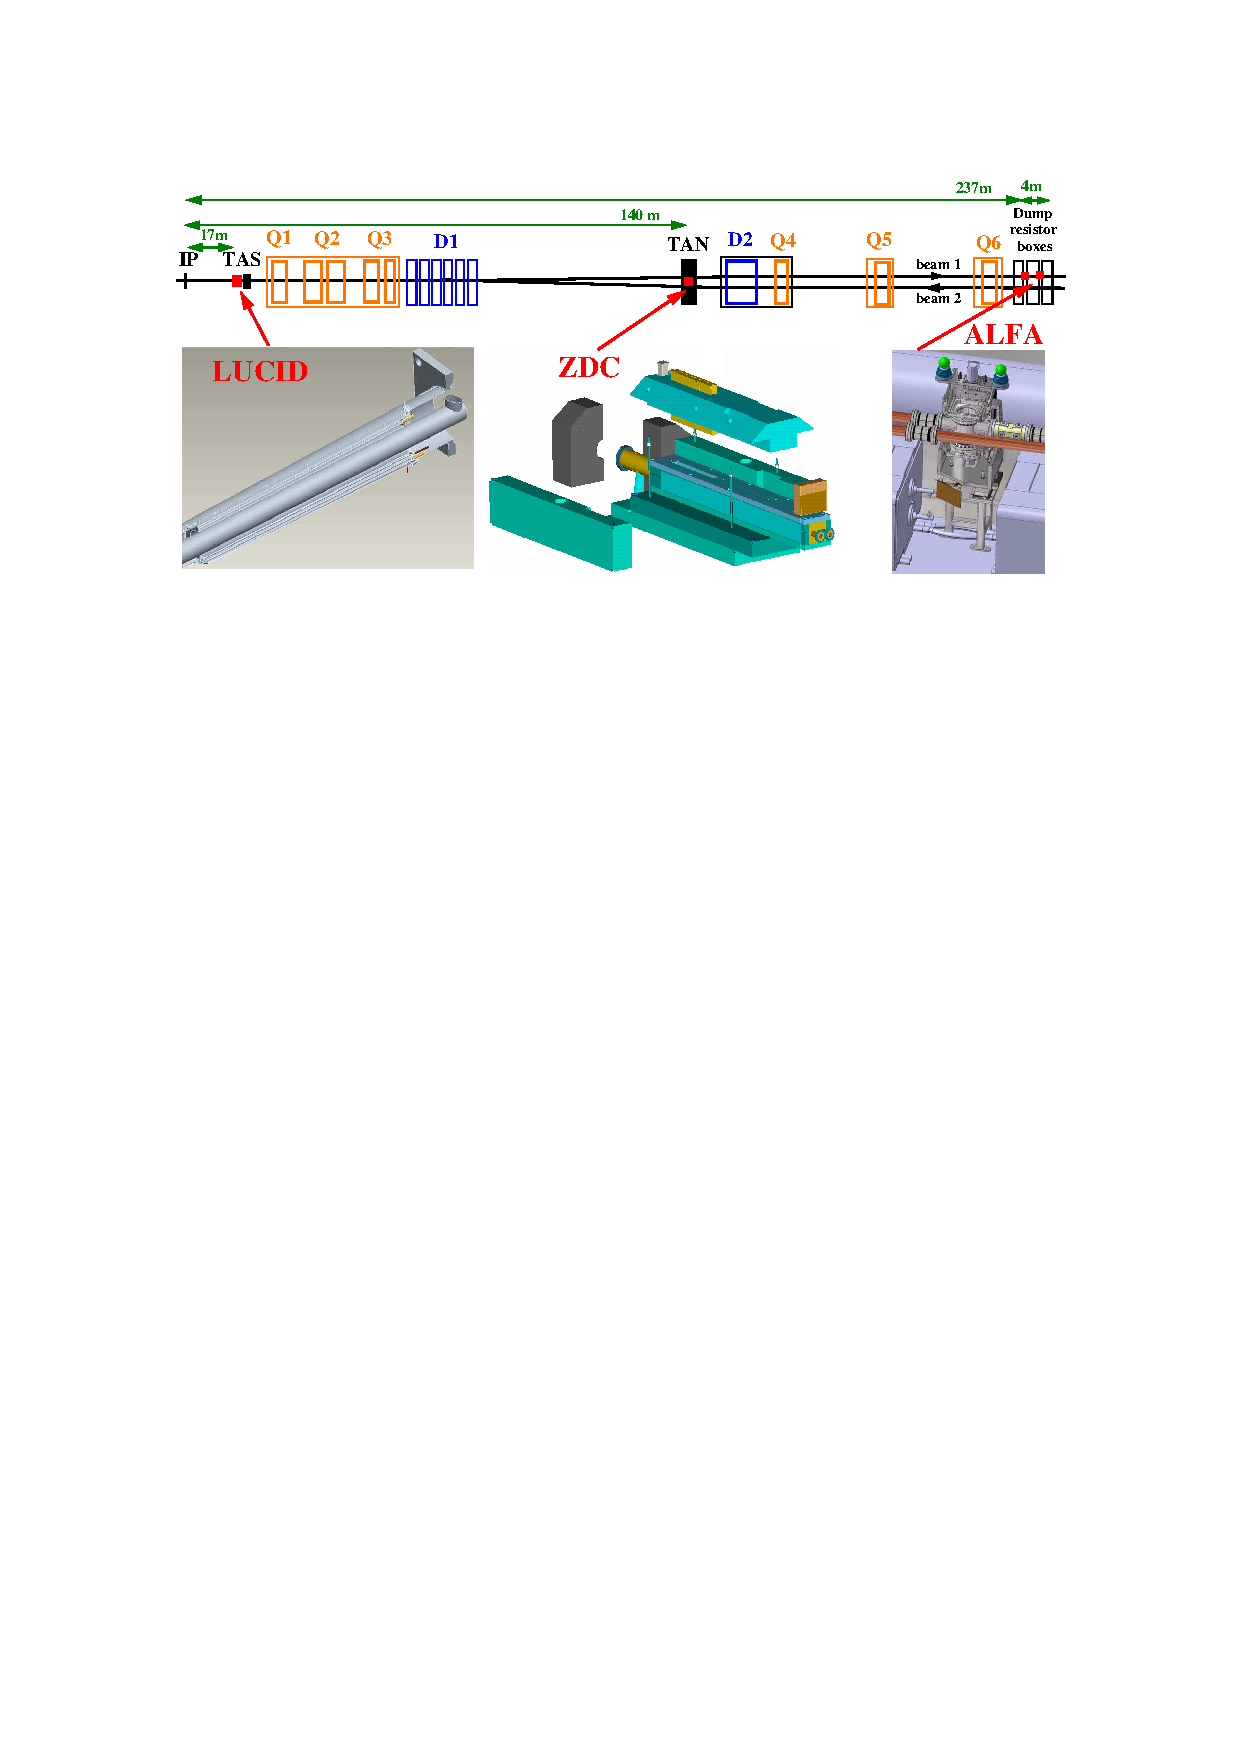
\includegraphics[width=0.75\textwidth]{figures/Chap3/Rizzi-Fig3-17-1.pdf}}
%\caption{Forward detectors in \gls{atlas}.}
%\label{fig:atlas:forward}
%\end{figure}

\subsubsection*{Tracker-based algorithms}

The \gls{id}, described in Section \ref{sec:atlas:id}, records the passage of charged particles as tracks. The number of such charged tracks in each bunch crossing is proportional to the luminosity, and can be used as ${<}\mu_\mathrm{vis}{>}$ if averaged over a \gls{lub}. 
During collisions, partial data, which are selected with a random trigger that has the same probability of firing for each colliding bunch, 
are recorded in a dedicated stream. Because of the high number of colliding bunches, to achieve enough statistical precision the luminosity is provided as integrated over the \gls{lub}; instead, during \gls{vdm} scans, bunch-by-bunch luminosity can be provided. 
% chiara: indicate which track types have been used in 2015--2016 and which in 2017
The reconstruction of the tracks used in this process is described in Section \ref{sec:reco:tracks}.

\subsubsection*{Bunch-integrating devices}

The long-term stability of the luminosity measurement provided by \gls{bcm}, LUCID and the track system is checked with devices that are sensitive to the flux of particles through the detector. This technique only allows to measure the instantaneous luminosity integrated over a time of a few seconds, and not bunch-by-bunch.

A subdetector capable of providing such measurement is \gls{tilecal}, described in Section \ref{sec:atlas:calo}. The current generated by the \glspl{pmt} is proportional to the total number of particles; this current is not read through the digital readout system, but through an integrator system sensitive to currents between 0.01 nA and 1.2 $\mu$A over a time window of 10--20 ms. The current induced in different cells varies largely with the cell position: the ones that receive a larger amount of particles are the ones around $|\eta|=1.25$ and in the inner part of the detector (as the hadronic shower is stopped while it passes through the calorimeter). The \gls{tilecal} luminosity measurement is not calibrated during \gls{vdm} scans, but is instead equalized to LUCID or the track measurement for one specific run, and the calibration constant between current and luminosity allows to measure the luminosity also in different runs. More details on the \gls{tilecal} luminosity measurement are given in 
Appendix \ref{app:pmt}. 

Additional systems used in the luminosity determination are the \gls{lar}-based calorimeters in the end caps, the electromagnetic one and the FCal. In both systems the high-voltage (HV) system maintains a constant voltage by supplying a continuous injection of current that counterbalances the voltage drop caused by the flux of particles in a certain sector. The measurement of this current provides a luminosity measurement. Also \gls{lar} systems are not calibrated during the \gls{vdm} scan, but each HV run is calibrated to the baseline luminosity algorithm over a physics run.  


\subsection{Trigger system}
\label{sec:cern:trigger}

With the nominal bunch spacing of 25 ns, the \gls{lhc} produces collisions at a frequency of 40 MHz. This exceeds by several orders of magnitude the current capability to write events to disk; therefore the \gls{atlas} \gls{tdaq} system selects and records the events that are considered interesting for analyses. The \gls{tdaq} system has been updated between Run 1 and Run 2 \cite{Aaboud:2016leb} and it currently consists of a  hardware \gls{lone} trigger and a single software-based \gls{hlt}. A schematic view of the Run 2 \gls{atlas} \gls{tdaq} system is shown in Figure \ref{fig:atlas:trig}. \gls{lone} is the first step in the chain, and reduces the output rate from 40 MHz to about 100 kHz. It uses reduced-granularity information from the calorimeter systems and from the muon \gls{rpc} and TGS to select events with interesting objects and saves the information about the \gls{roi}. \gls{lone} has a latency time of 2.5 $\mu$s; this corresponds to about 100 collisions, whose information has to be temporarily stored in buffers before the \gls{lone} \gls{ctp} finalizes a decision based on the inputs from the \gls{lonecalo}, \gls{lonemuo} and the \gls{lonetopo}. 

During Run 1 the \gls{hlt} consisted of two separate levels that in Run 2 have been merged to have a simpler setup and better resource sharing. The \gls{hlt} uses information with finer granularity from the calorimeter systems, precision tracking from the muon spectrometer and tracking information from the \gls{id}, not available for \gls{lone}. The \gls{hlt} reduces further the event rate to about 1 kHz, and has a processing time of about 0.2 s per each event. 

A trigger chain is a set of selections that characterize a certain trigger object, and the list of all available trigger chains defines the trigger menu; some of the items on the menu are unprescaled, which means all the events firing that trigger are stored, while others are associated to a prescale constant $P$ such that only a fraction $1/P$ of the events firing the trigger are stored.

\begin{figure}[ht]
\centering
\subfigure[]{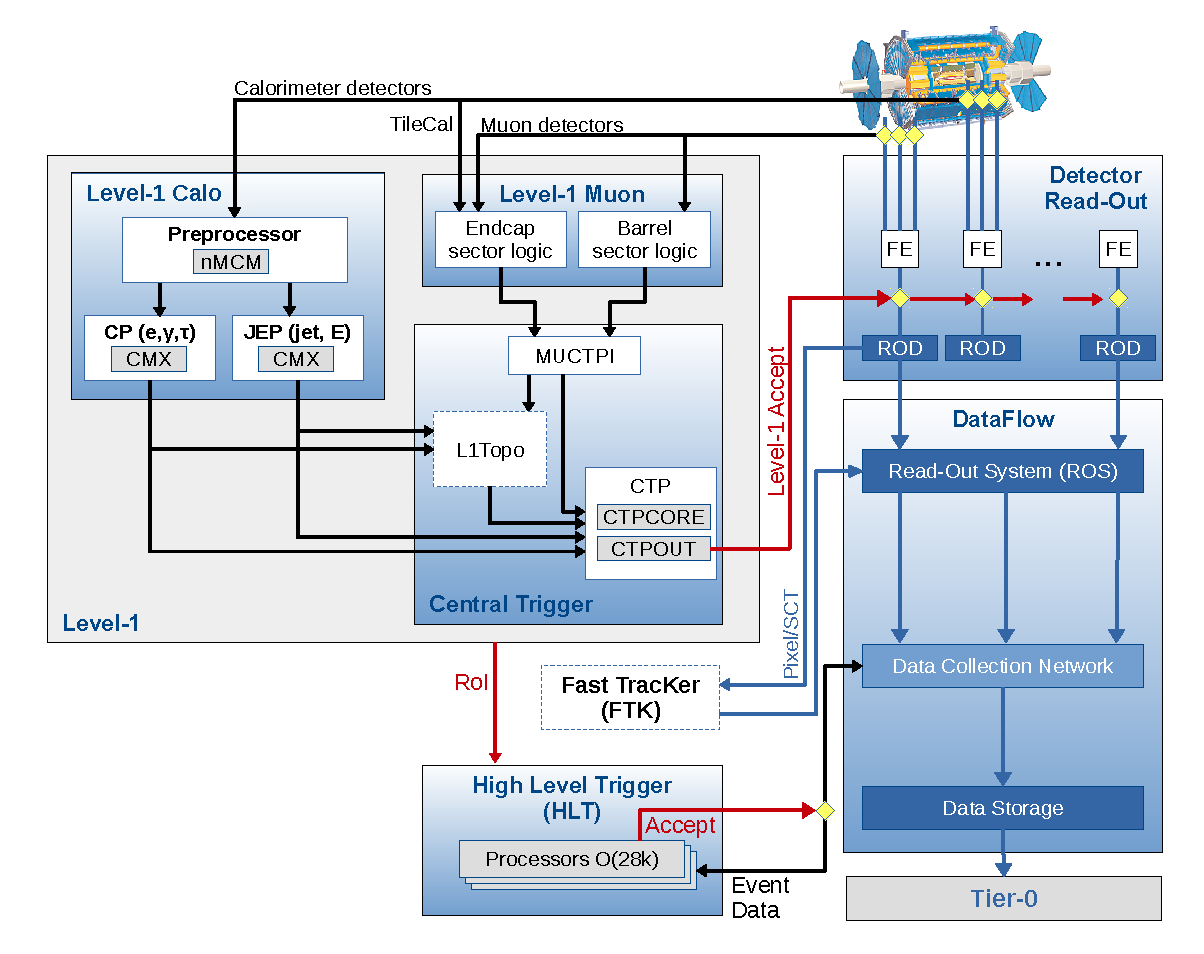
\includegraphics[width=0.9\textwidth]{figures/Chap3/Rizzi-Fig3-18-1.pdf}}
\caption{Schematic view of the Run 2 \gls{atlas} \gls{tdaq} system. Figure from Ref. \cite{Aaboud:2016leb}.}
\label{fig:atlas:trig}
\end{figure}


\subsection{ATLAS operation}

\gls{atlas} has been successfully recording the collision data delivered by the \gls{lhc} in Run 1 and Run 2. Figure \ref{fig:atlas:lumi1} shows the cumulative luminosity delivered by the \gls{lhc} between the declaration of stable beams and the request to put the detector in standby for beam dump  as well as the luminosity recorded by \gls{atlas} in 2015, 2016 and 2017, which is the dataset used in the analyses described in this thesis. The difference between the delivered and recorded luminosity derives from inefficiencies of the data acquisition system and from the ``warm start'' procedure: 
the pixel and \gls{sct} high voltage and the preamplifiers of the pixel detector are turned on after the start of stable beams \cite{LumiTwiki}.

\begin{figure}[ht]
\centering
\subfigure[]{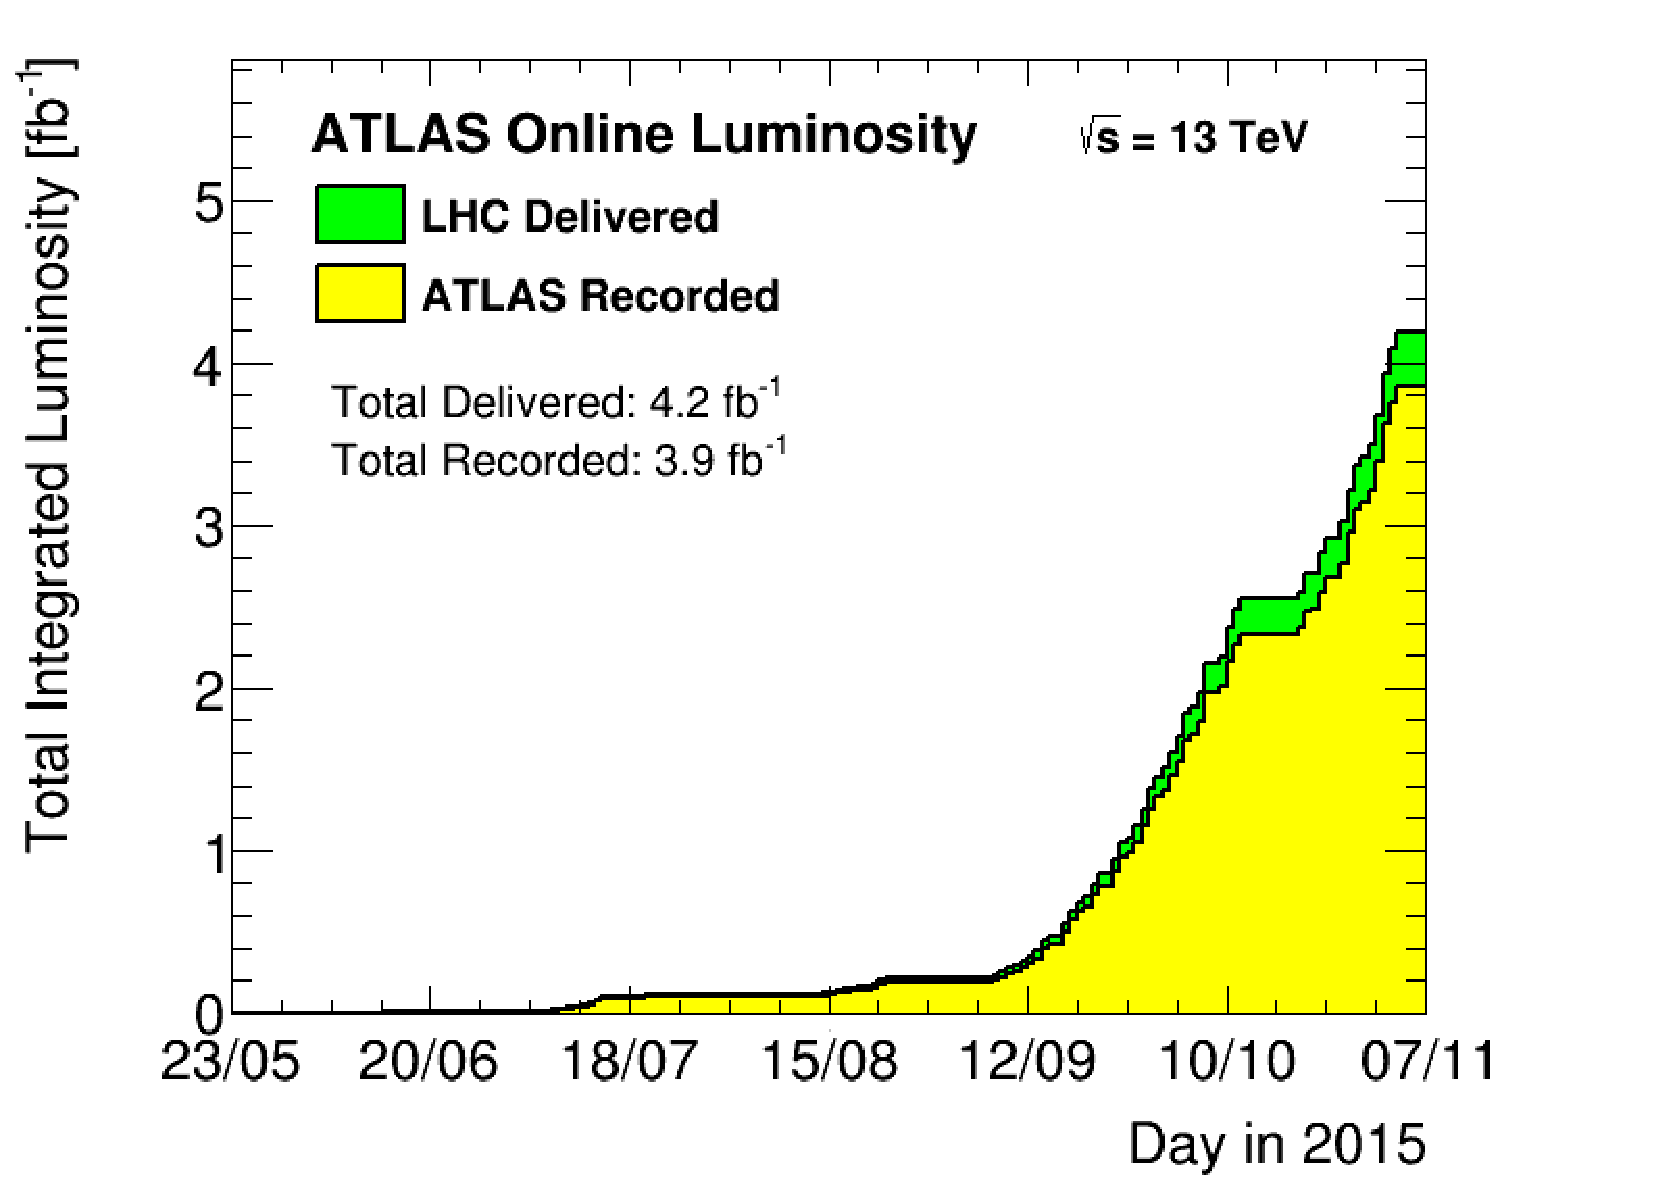
\includegraphics[width=0.48\textwidth]{figures/Chap3/Rizzi-Fig3-19-1.pdf}\label{fig:atlas:lumi1:a}}
\subfigure[]{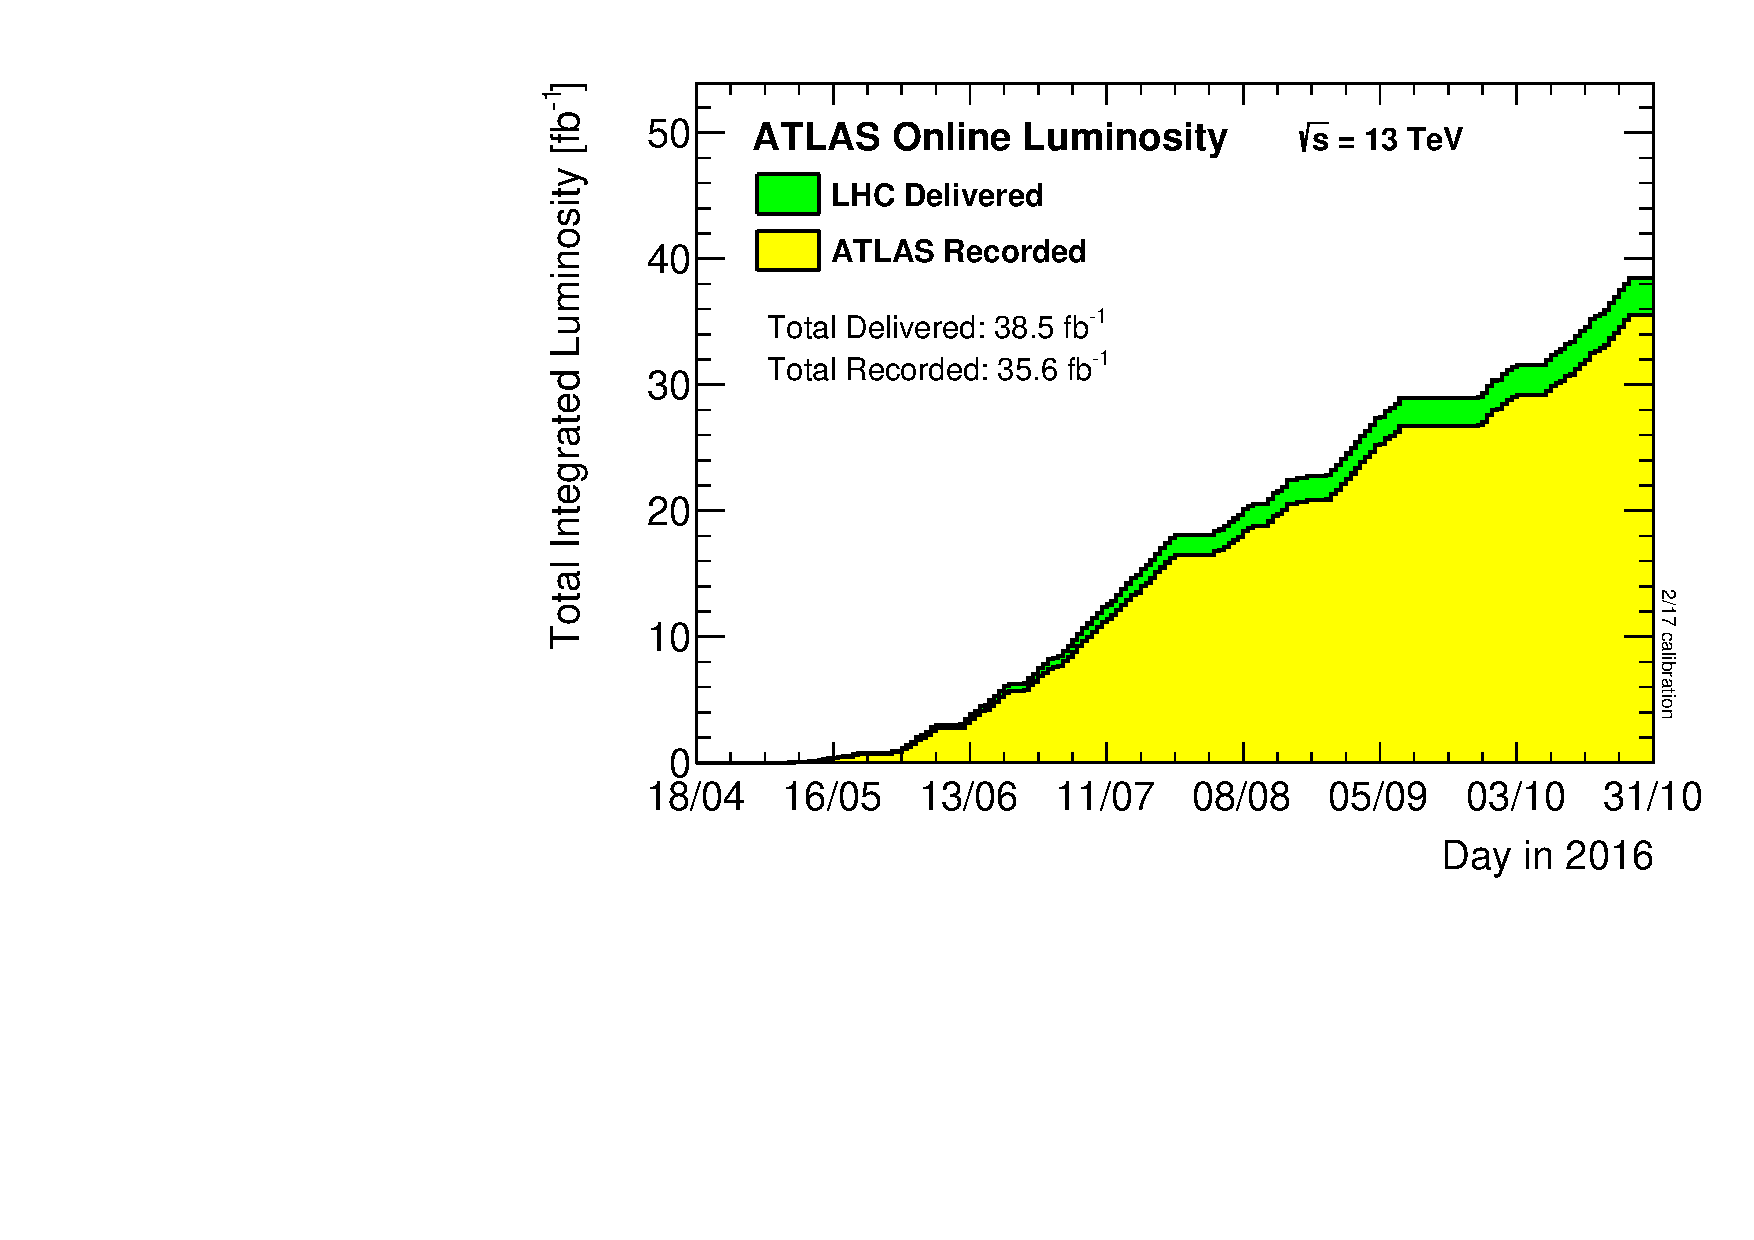
\includegraphics[width=0.48\textwidth]{figures/Chap3/Rizzi-Fig3-19-2.pdf}\label{fig:atlas:lumi1:b}}\\
\subfigure[]{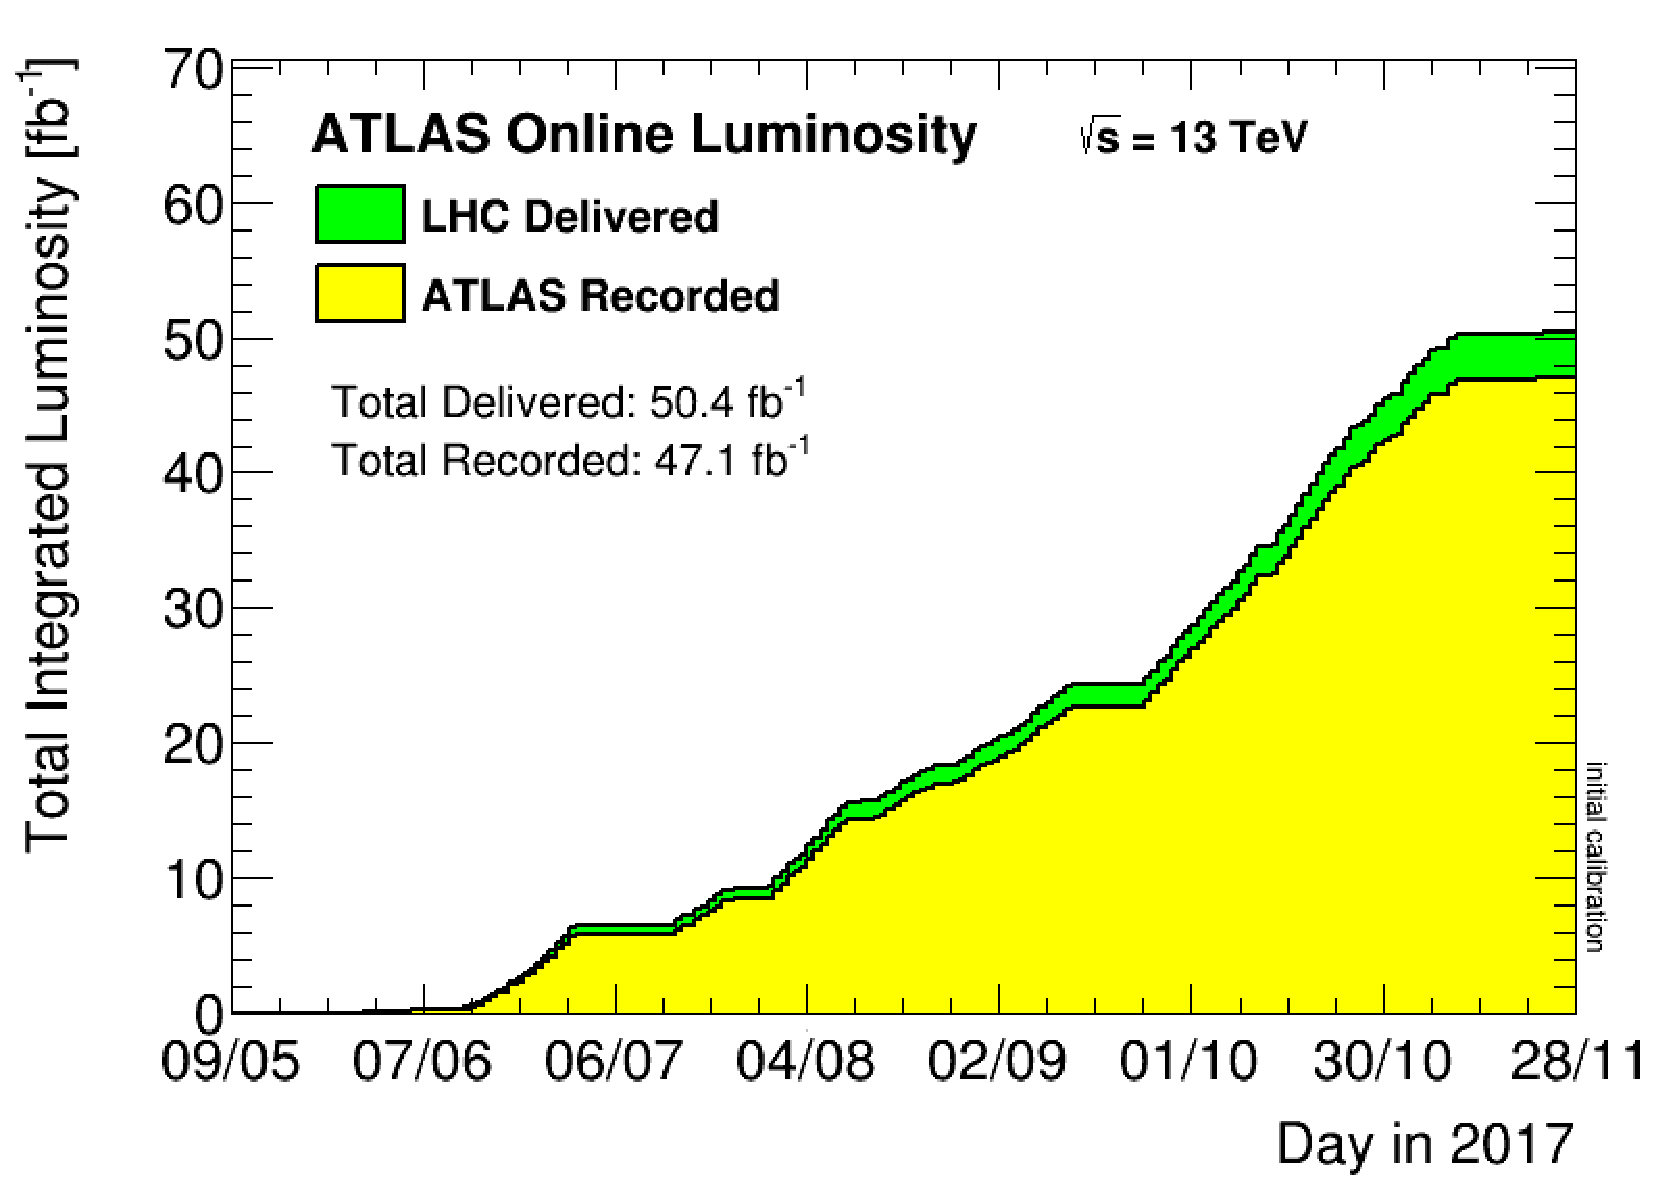
\includegraphics[width=0.48\textwidth]{figures/Chap3/Rizzi-Fig3-19-3.pdf}\label{fig:atlas:lumi1:c}}
\subfigure[]{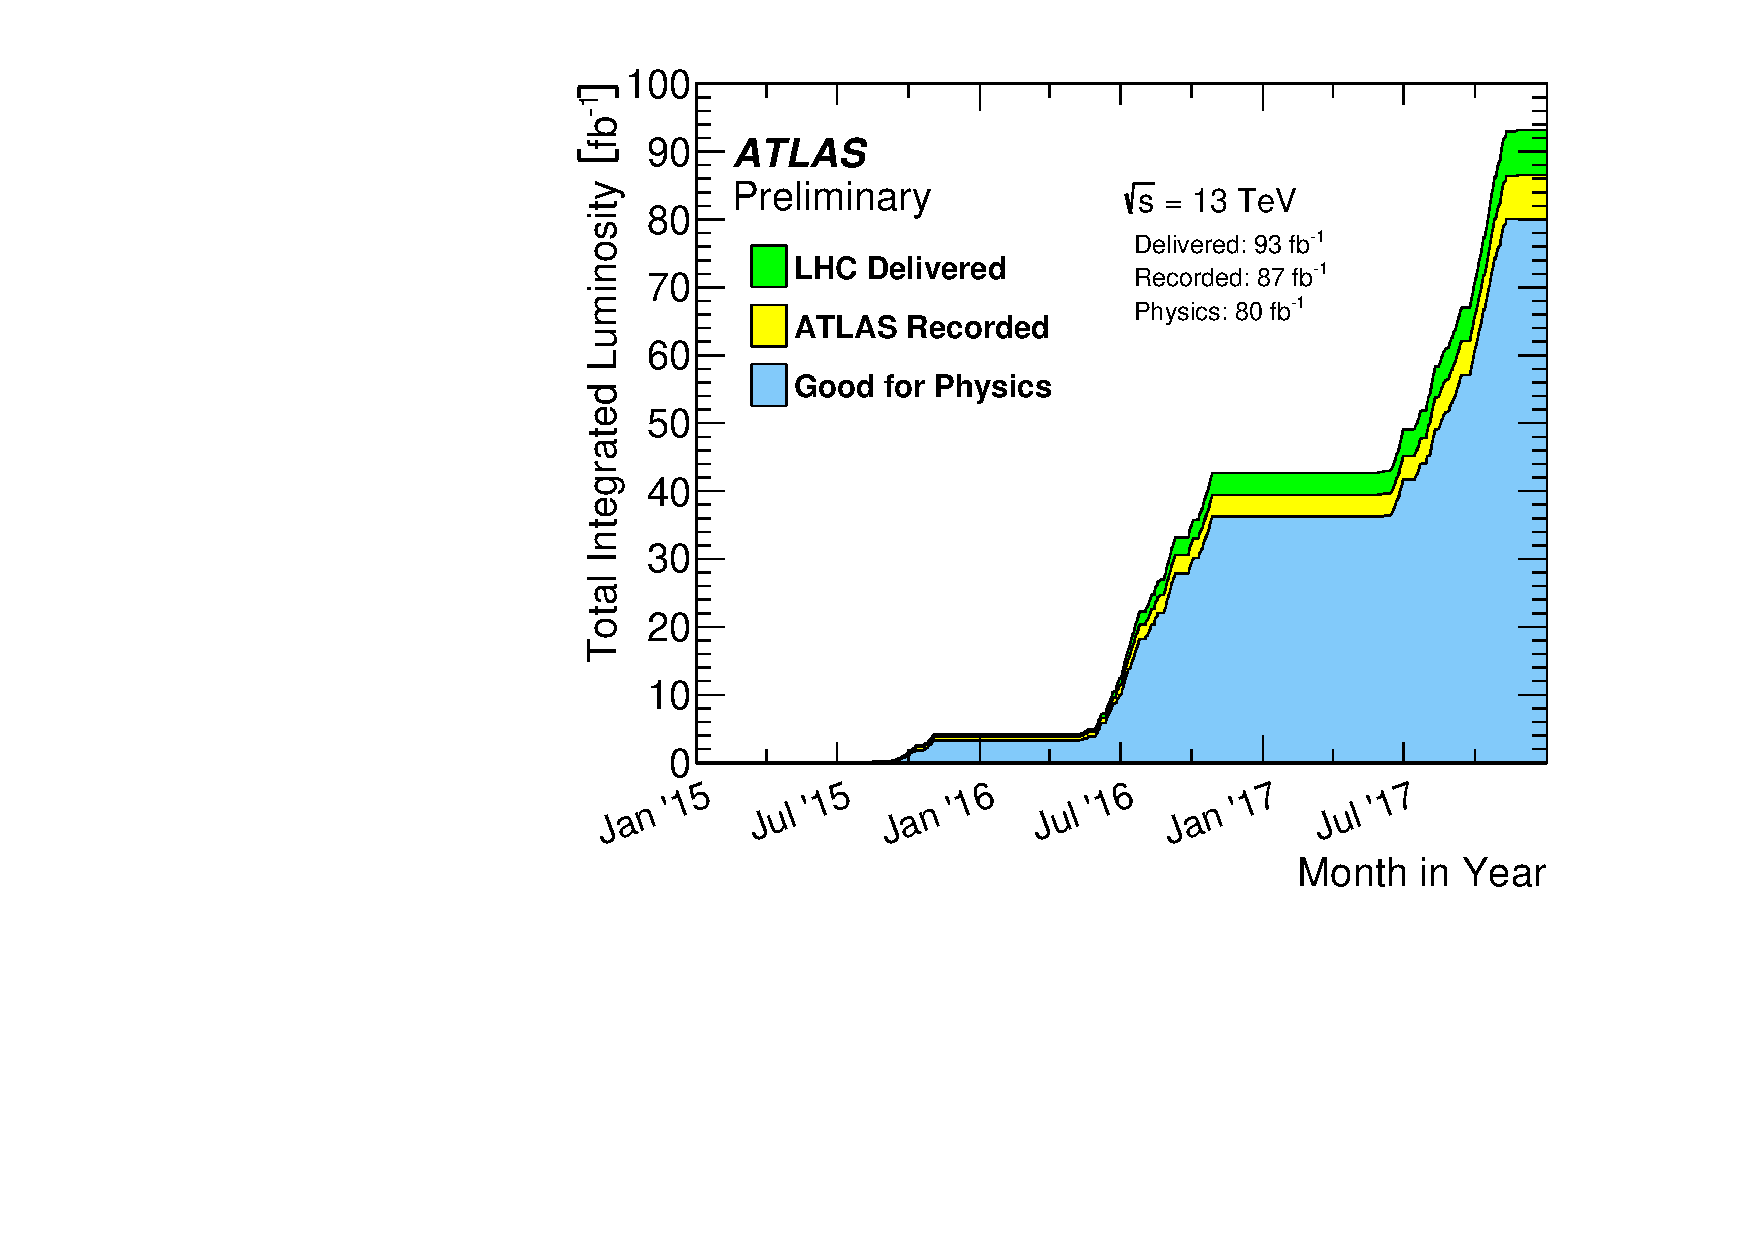
\includegraphics[width=0.48\textwidth]{figures/Chap3/Rizzi-Fig3-19-4.pdf}\label{fig:atlas:lumi1:d}}
\caption{Cumulative luminosity versus time delivered to (green) and recorded by \gls{atlas} (yellow) during stable beams for pp collisions at $\sqrt{s}=13$ TeV in \subref{fig:atlas:lumi1:a} 2015, \subref{fig:atlas:lumi1:b} 2016, 
and \subref{fig:atlas:lumi1:c} 2017. \subref{fig:atlas:lumi1:d} Cumulative luminosity versus time in 2015--2017 certified to be good quality data (blue). Figure from Ref. \cite{LumiTwiki}.}
\label{fig:atlas:lumi1}
\end{figure}

Not all the recorded luminosity can be used for physics analyses, as most of these require a good state of all the detector subsystems. This is checked for each luminosity block; the ones with poor detector conditions are disregarded, while the ones that pass this criteria form the \gls{grl}, which imposes requirements on the quality of the beams and of the detector. Figure \ref{fig:atlas:lumi1:d} shows the total cumulative luminosity for the 2015--2017 period, highlighting the portion that enters the \gls{grl}. 


\clearpage 
\bibliographystyle{atlasBibStyleWithTitle}
\addcontentsline{toc}{section}{Bibliography}
\bibliography{main} 

%\glsresetall
\glsunset{atlas}
\glsunset{cms}
\chapter{Proton-proton interactions and their simulation}
\label{chap:event:MC}

Proton-proton interactions at the \gls{lhc} are complex processes that span very different energy scales. 
In order to interpret the experimental data it is essential to develop a good understanding of the physics involved in \gls{pp} collisions. 
The ability to simulate the various processes is crucial to compare the observed data with the theory predictions.
Section \ref{sec:ppint} focuses on the description of our understanding of a \gls{pp} collision, while Section \ref{sec:eventsimul} 
discusses the event-simulation process; 
the main \gls{mc} generators used in the \gls{atlas} Collaboration are described in Section \ref{sec:mcgen}, and Section \ref{sec:detsim} touches briefly on the topics of detector simulation and data-driven corrections.



\section{Proton-proton interactions}
\label{sec:ppint}

In hard-scattering processes, where the momentum transfer is much higher than the proton mass \cite{Butterworth:2012fj}, 
a \gls{pp} collision is easier to understand in terms of interactions between the constituents of the protons, quarks and gluons, 
collectively referred to as partons. A schematic view of a \gls{pp} event is shown in Figure \ref{fig:sim:pp2}. In this particular example, the interaction between a quark and a gluon leads to a final state with a $Z$ boson and jets. 

\begin{figure}[h]
\begin{center}
%  \subfigure[]{
%    \label{fig:Comb_syst:pt}
    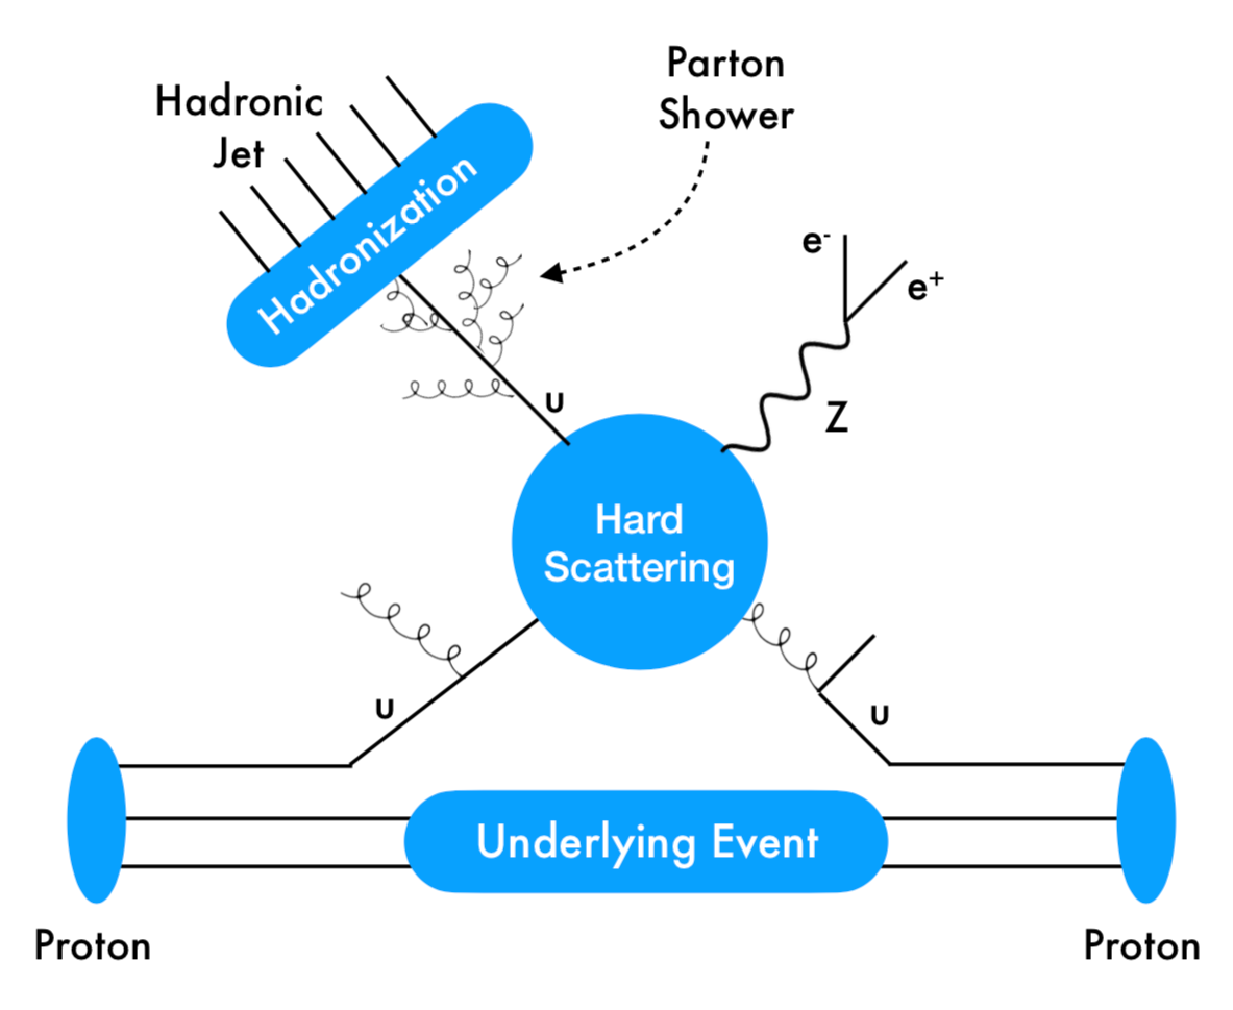
\includegraphics[width=0.68\textwidth]{figures/springer/mc_simul}
%  }
\end{center}
 \caption{Schematic representation of a \gls{pp} collision, involving a quark-gluon scattering that leads to a final state consisting of a $Z$ boson and a hard jet.}
  \label{fig:sim:pp2}
\end{figure}

As can be appreciated from the figure, the hard process, which can be computed in perturbation theory, takes place between two of the proton's partons; the probability that a gluon or a specific quark type takes part in the hard scattering is related to the \glspl{partdf}, discussed in Section \ref{sec:ppint:hardscatter}. If the products of the hard scattering are quarks or gluons, they first of all loose energy by radiating other gluons (which in turn can generate quark-antiquark pairs through gluon splitting) in the process of parton shower;
successively they evolve to stable hadrons in the lower-energy hadronization process, which we can describe only through phenomenological models.
This picture is further complicated by the fact that also initial-state quarks and gluons can radiate. Also, the other partons not contributing to the hard scattering can interact, originating what is referred to as the underlying event. 

\subsection{Factorization theorem}
\label{sec:ppint:hardscatter}

The hard scattering between the partons inside the proton takes place in a kinematic regime where the strong coupling constant, $\alpha_s$, 
is small and therefore the partonic cross-sections can be computed in perturbation theory. 
Thanks to the factorization theorem \cite{doi:10.1146}, the generic production cross-section for a final state $X$ can be expressed in terms of the partonic cross-section $\hat\sigma$ as:

\begin{equation}
  \sigma(pp\rightarrow X) = \sum_{i,j} \int dx_1 dx_2\, 
     f_{i}(x_1,\mu_F^2)\, f_{j}(x_2,\mu_F^2)\, 
     \hat\sigma_{ij\rightarrow X}(x_1 x_2 s, \mu_R^2, \mu_F^2) \; .
  \label{eq:general-cross-section}
\end{equation}
The $i$ and $j$ indexes run over all possible partons, and $f_{i}(x_1,\mu_F^2)$ is the \gls{partdf} for the parton of type $i$, representing 
the distribution of probability for that parton to carry a fraction $x_1$ of the proton momentum when the proton is probed at a scale $\mu_F$
(factorization scale). The partonic cross-section, $\hat\sigma_{ij\rightarrow X}$, is computed at the partonic center of mass energy \cmpart;   
it has to be noted that \cmpart is lower than the total center of mass energy, as 
$\hat\sigma = x_1  x_2  s$, 
where $x_1$ and $x_2$ are the fraction of the proton momentum that is carried by each of the two partons.
Although the partonic cross-section depends on $\mu_F$ and on the renormalization scale $\mu_R$, 
which is the scale used for the evaluation of $\alpha_s$, 
when considered at all orders in perturbative \gls{qcd} this dependence disappears.
Higher-order calculations exhibit a reduced scale dependence, and are therefore used whenever available. 


% factorization theorem 


%\begin{figure}[h]
%\begin{center}
%  \subfigure[]{
%    \label{fig:Comb_syst:pt}
%    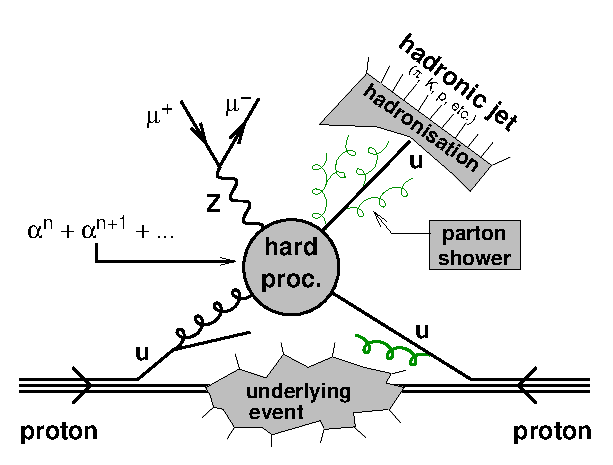
\includegraphics[width=0.48\textwidth]{figures/simul/ppcoll2}
%  }
%    \subfigure[]{
%    \label{fig:Comb_syst:pt}
%    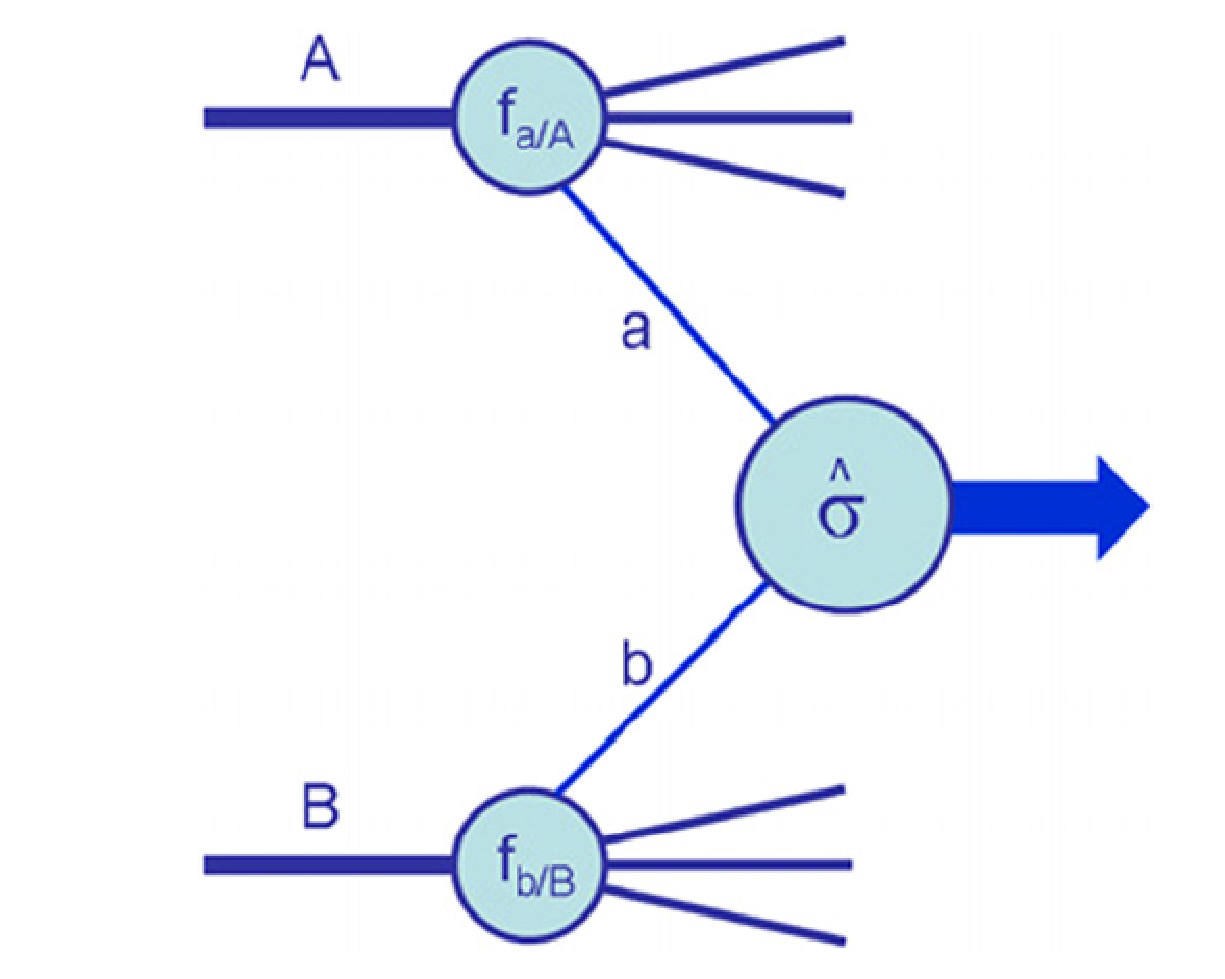
\includegraphics[width=0.48\textwidth]{figures/simul/ppcoll}
%  }
%\end{center}
% \caption{Diagrammatic structure of a generic hard-scattering process. Figure from Ref. \cite{Campbell:2006wx}.}
%  \label{fig:sim:pp}
%\end{figure}

\subsection{Parton density functions}
\label{sec:protpdf}

The partons inside the proton cannot be observed as free particles, and therefore their \glspl{partdf} cannot be computed with
perturbative \gls{qcd}. In particular, for a given scale, it is not possible to predict theoretically the probability distribution 
of the parton's momentum fraction. Instead, once the \glspl{partdf} are known at a certain scale, their energy evolution is 
determined by the equations derived independently by Dokshitzer \cite{Dokshitzer:1977sg} , Gribov and Lipatov \cite{Gribov:1972ri}, and Altarelli and Parisi \cite{ALTARELLI1977298} (DGLAP equations):

\begin{equation}
\begin{aligned}
\frac{\partial q(x,Q^2)}{\partial {\rm log}Q^2}~&=~\frac{\alpha_s}{2\pi}~\left( P_{qq} \otimes q~+~P_{qg} \otimes g \right) \, ,\\
\frac{\partial g(x,Q^2)}{\partial {\rm log}Q^2}~&=~\frac{\alpha_s}{2\pi}~\left( \sum_i P_{gq} \otimes (q_i+\bar{q}_i)~+~P_{gg} \otimes g \right) \; . \nonumber
\label{eq:glap1}
\end{aligned}
\end{equation}

\noindent In the expressions above, $q(x,Q^2)$ and $g(x,Q^2)$ denote the quark and gluon \glspl{partdf} respectively, 
$P_{ij}$ describes the $i \to j$ parton splitting function, 
which corresponds to the probability of the outgoing parton $j$ 
to be emitted at a virtuality scale $Q^2$ and carry a fraction $x$/$y$ of the mother parton momentum, 
and $\otimes$ is a symbol for the convolution integral:
\begin{equation}
P \otimes f \equiv \int^1_x\frac{dy}{y}f_q(y)~P\left(\frac{x}{y}\right) \; . \nonumber
\end{equation}

As mentioned above, the \glspl{partdf} have to be determined experimentally. This is done by several collaborations through fits (with typically 10 to 30 parameters) to experimental data. 
As an example, Figure \ref{fig:sim:pp} shows the \gls{nlo} \glspl{partdf} obtained by the \gls{atlas} Collaboration at Q$^2$ = 10 GeV$^2$. 
Comparing this with \glspl{partdf} at different Q$^2$ (e.g. in Ref. \cite{Martin:2009iq}), it can be observed that, with the increase of Q$^2$, the shape of the \glspl{partdf} changes to favor lower $x$ values. At low $x$ values the gluon \gls{partdf} is dominating (and this effect increases with Q$^2$), while for high $x$ values the \glspl{partdf} of the valence quarks are more relevant.

\begin{figure}[h]
\begin{center}
    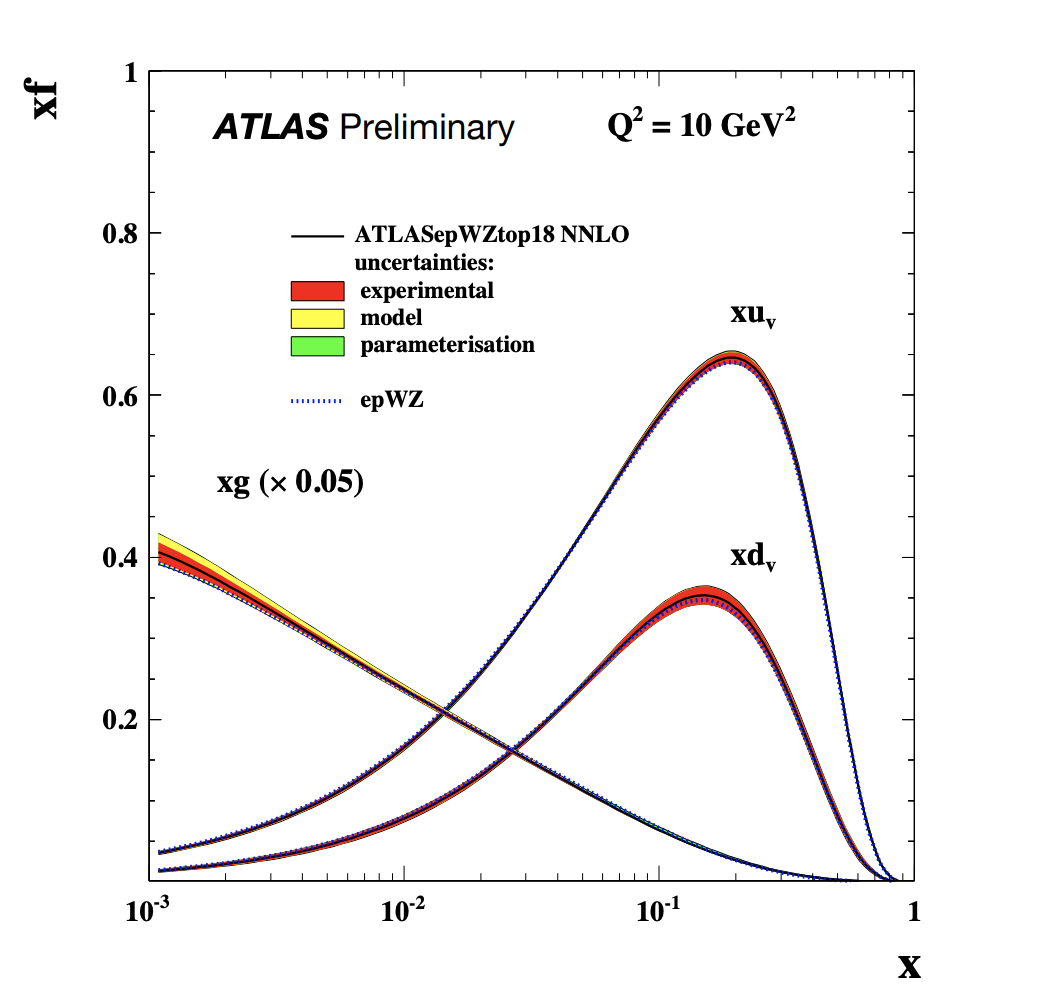
\includegraphics[width=0.65\textwidth]{figures/springer/pdf}
\end{center}
\caption{Gluon and valence \glspl{partdf} at Q$^2$ = 10 GeV$^2$. 
Figure from Ref. \cite{ATL-PHYS-PUB-2018-017}.
%Figure from Ref. \cite{Martin:2009iq}.
}
 \label{fig:sim:pp}
\end{figure}


\section{Event simulation}
\label{sec:eventsimul}

The main steps in the simulation of a \gls{pp} collision consist of:
\begin{itemize}
\item Computation of the \glspl{me} for the hard process.
\item \Gls{psh} evolution and matching between \gls{psh} and \glspl{me}.
\item Hadronization and decay of unstable particles.
\item Simulation of the underlying event and pileup.
\end{itemize}
In the next sections, each step is summarized in its main features.

\subsection{Matrix element}

As discussed e.g. in Ref \cite{Skands:2011pf}, the partonic cross-section for the production of the final state $X$ starting from the partons $i$ and $j$, necessary to compute
Equation \ref{eq:general-cross-section}, can be expressed at all orders as:
\begin{equation}
\hat\sigma_{ij\rightarrow X} = \sum_{k=0}^\infty \int d\Phi_{X+k} | \sum_{l=0}^\infty \mathcal{M}_{X+k}^{(l)}|^2 \; .
\label{eq:xsec_matrix}
\end{equation}
\noindent In this expression, the index $k$ denotes the number of final-state quarks and gluons produced in addition to $X$ (legs) and $\mathcal{M}_{X+k}^{(l)}$
the amplitude to produce the final state $X+k$ computed with $l$ virtual loops. 
These sums can not be computed to infinity, and the perturbative order of the cross-section 
is identified by the number of extra partons and by the number of loops. 
In particular:
\begin{itemize}
\item The lowest possible order for the calculation of $\hat{\sigma}_{ij \rightarrow X}$ is the \gls{lo}, where $k=l=0$.
\item $l=0$, $k=n$ represents the \gls{lo} computation for the production of $X$ + $n$ jets.
\item $k+l \leq n$ corresponds to a N$^n$LO prediction for the production of $X$, while N$^{n-k}$LO for the production of $X$ in association with $k$ jets.
\end{itemize}

At each order, the computation of the \glspl{me} implies a choice of the factorization and renormalization scales 
($\mu_F$ and $\mu_R$, respectively). 
These scales are not predetermined, and are typically set to values related to the characteristic energy scale of the considered physical process. 
The impact of this subjective choice is taken into account by evaluating each production cross-section at different scales (typically varying the nominal scale by a factor of two up and down), and assigning the difference as a systematic uncertainty in the cross-section estimate.


\subsection{Parton shower}

A theorem by Kinoshita, Lee and Nauenberg (KLN theorem) \cite{Kinoshita:1962ur,Lee:1964is} guarantees that, 
when computing inclusive cross-sections, the logarithmic divergences arising from collinear splitting cancel against the virtual corrections order by order in perturbation theory. 
This does not hold anymore when we are interested in the computation of a differential cross-section, for example with a specific number of accompanying final-state extra partons, 
as it could be the case $l=0$, $k=1$ in Equation \ref{eq:xsec_matrix}. 
In this case, the kinematic of the basic inclusive event is simulated at fixed order, and the \gls{qcd} emission process (splitting) is carried out by the \gls{psh} algorithms \cite{Fox:1979ag}, which generate an ordered sequence of emissions with decreasing angle or energy; the \gls{psh} approximation consists in retaining only singular parts of the \glspl{me}, namely those corresponding to low angles and energies, obtaining a \gls{ll} accuracy.
Starting from the cross-section for the production of $n$ particles, the cross-section for the production 
of $n+1$ particles is calculated based on the parton splitting function $P_{ij}$ (described in Section \ref{sec:protpdf}):
\begin{equation}
d\sigma_{n+1} \approx d\sigma_n \, \frac{ \alpha_s }{2 \pi } \, \frac{dt}{t}  \,  P_{ij}(z, t) \, dz \; . \nonumber
\end{equation}
The probability for a parton to evolve from an energy $t$ to a lower energy $t'$ without splitting is encoded in the Sudakov form factor:
\begin{equation}
  \Delta_i(t,t')=\exp\left(-\sum_{j\in\{q,g\}}\,
  \int_t^{t'}\frac{{\rm{d}}\bar{t}}{\bar{t}}\int_{z_{\rm min}}^{z_{\rm max}}{\rm{d}} z\,
  \frac{ \alpha_s }{2 \pi } \, \frac{1}{2} \, P_{ij}(z, t) \right) \;,
  \label{eq:sudakov_intro}
\end{equation}

There are three types of emission processes that are described by the \gls{psh}: $g \rightarrow q\bar{q}$, $g \rightarrow gg$ and $q \rightarrow q g$.
Equation \ref{eq:sudakov_intro} is sampled with \gls{mc} techniques to produce the sequence of splittings, until the hadronization scale is reached;
this describes \gls{fsr}.

Also incoming particles can emit extra partons, giving rise to \gls{isr}. 
While in the case of \gls{fsr} the first emissions are harder than subsequent ones, 
for \gls{isr} the ordering is inverted, and the showering is performed with a backwards-evolution algorithm \cite{Sjostrand:1985xi}.

\subsection{Matching}

When a process F is simulated with \gls{lo} \glspl{me} plus \gls{psh}, as illustrated in the left diagram in Figure \ref{fig:sim:matching}, 
the hardest extra jet is described at \gls{ll} accuracy. 
One might wish to improve the accuracy of the description of the event by adding the \gls{lo} \glspl{me} 
for the process F with the addition of one extra parton (F+1), as in the second diagram in Figure \ref{fig:sim:matching}. 
In this figure, the boxes are only partially filled to indicate the phase-space restriction 
necessary to deal with the divergence of the F+1 \glspl{me}. 
The naive addition of these two pieces leads to double counting of configurations. 
This double-counting problem worsens with the increase of the number of extra legs that we want to add to the \glspl{me}.

Different methods have been designed to match \glspl{me} to showers such that, for each order in perturbation theory, double-counting is avoided. The three main strategies are \cite{Giele:2011cb}:
\begin{description}
\item[Unitarity] This approach consists in correcting the shower splitting functions by multiplicative factors obtained as the ratio of the \gls{me} to \gls{psh} approximation:
$$
\rm{Matched} = \rm{Approximate}\frac{\rm{Exact}}{Approximate} \; .
$$
\noindent When these correction factors are inserted in the shower evolution, they guarantee that the shower evolution of the process F describes correctly also the F+1 \glspl{me}, without actually adding the F+1 sample. This strategy has traditionally been worked out only for one extra parton emission. 

\item[Subtraction] The subtraction approach consists in correcting the \gls{psh} by the difference between the \glspl{me} and the \gls{psh}:
$$
\rm{Matched} = \rm{Approximate} + (\rm{Exact}- \rm{Approximate}) \; .
$$

\noindent With this strategy, the corrections are not resummed and the events are weighted. This is the strategy used in \mcatnlo \cite{Frixione:2002ik,Frixione:2003ei,Frixione:2008ym}, and the \Powheg method \cite{Frixione:2007vw} is a hybrid between this and the unitarity approach.

\item[Slicing] The slicing approach divides the phase space into two regions: one described mainly by the \glspl{me} (by vetoing shower emissions below a cutoff scale, the matching scale), and one mainly by the \gls{psh}:
\begin{equation*}
\begin{split}
 {\rm{Matched (above \; matching \;  scale)}} &\approx {\rm{Exact}} (1 + {\mathcal{O}} ( \alpha_s)) \; , \\
{\rm{Matched (below \; matching \;  scale)} } &= {\rm{Approximate}} + ({\rm{Exact}}- {\rm{Approximate}})  \\
& \approx {\rm{Approximate}}    \; , \nonumber
\end{split}
\end{equation*}


\noindent where the last approximation holds because, below the matching scale, the \glspl{me} and the \gls{psh} give similar results. 
With the slicing strategy, the corrections are not resummed and the events are weighted, but the weights are all positive. This approach can be extended beyond the first extra emission. 
Examples of this approach are the CKKW \cite{Catani:2001cc} and MLM \cite{Mangano:2006rw,Mrenna:2003if} prescriptions. The MLM approach at \gls{nlo} is known as FxFx \cite{Frederix:2012ps}. 

\end{description}


\subsection{Hadronization}

At the end of the shower we have emissions at very low energy, which correspond to high values of the strong coupling constant. 
When the strong coupling becomes of order unity, the interaction is very strong and this is presumably what causes the confinement of the colored partons into colorless hadrons (primary hadrons), 
that can in turn decay to secondary hadrons. This transition is described through phenomenological models since the hadronization scale, that corresponds also to the \gls{ir} cutoff of the parton shower, is outside the perturbative regime of \gls{qcd}. At the end of the shower, the color, flavor and momentum distributions are already organized, and the hadronization process can only cause a local redistribution.
The two main hadronization models used in \gls{mc} generators are:

\begin{description}
\item[String Model] The string model \cite{Artru:1974hr} 
%, whose schematic is depicted in Figure \ref{fig:string_model}, 
is based on linear confinement: the potential energy between two colored particles increases linearly with their distance, when the distance is greater than about 1 fm (while at shorter distances also a Coulomb term is present). The term ``string model'' comprises several different models, among which the most used nowadays is the Lund model \cite{Andersson:1983ia,Andersson:1998tv}. 
A color string forms that joins the final state in a string configuration of field energies, and hadrons originate from the breakups of the string. The proportionality constant of the linear inter-quark potential can be measured from quarkonia spectra or from lattice \gls{qcd}, and results to be $\approx$ 1 GeV/fm.
The main difference between quarks and gluons resides in the fact that, while quarks are connected to one single string, gluons are connected to two strings and have therefore a rate for hadron production twice that of quarks. 
% chiara: describe the main steps of the string model hadronization
The fragmentation function determines the probability of a given hadron to carry a certain fraction of the available momentum. In the Lund model the form of the fragmentation function is constrained by the left-right symmetry necessary to make the model independent of the sequence of string breakups. The resulting function depends on the mass and \pt of the hadron, leading to heavier hadrons carrying on average a higher fraction of the momentum.

\item[Cluster Model] The cluster model  
%, sketched in Figure \ref{fig:cluster_model}, 
is based on the preconfinement property of \gls{qcd}. 
Color-singlet combinations of partons, referred to as clusters, are formed during the parton shower,  
and then decay to (possibly unstable) hadrons. 
Heavier clusters may first split through non-perturbative processes, and decay first to a pair of clusters or to a cluster and a hadron; 
this process continues until all clusters are transformed into hadrons. 
The mass distribution of the preconfined clusters results to be independent of the scale and nature of the original hard process. This universal distribution of the cluster mass peaks below 1 GeV, with a tail that extends to above 10 GeV.

\end{description}

%\begin{figure}[h]
%\begin{center}
%  \subfigure[]{
%    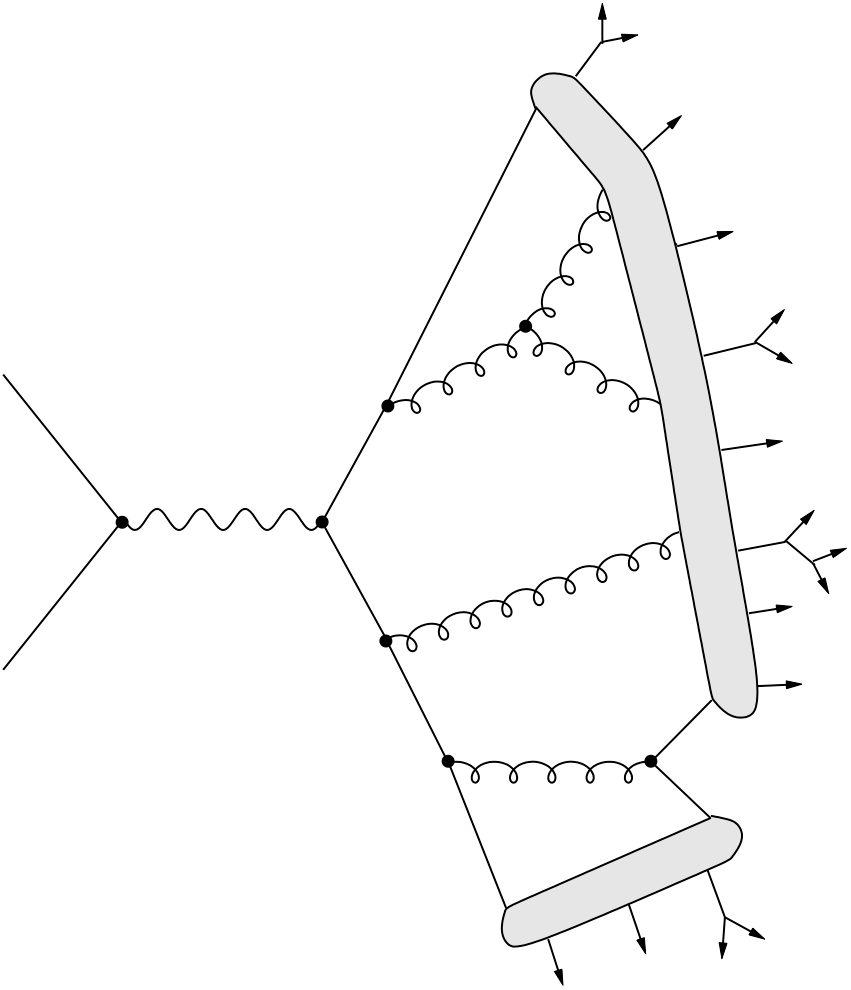
\includegraphics[width=0.35\textwidth]{figures/simul/Figures_MonteCarlo_string_had.pdf}
 %       \label{fig:string_model}
%  }
%    \subfigure[]{
 %   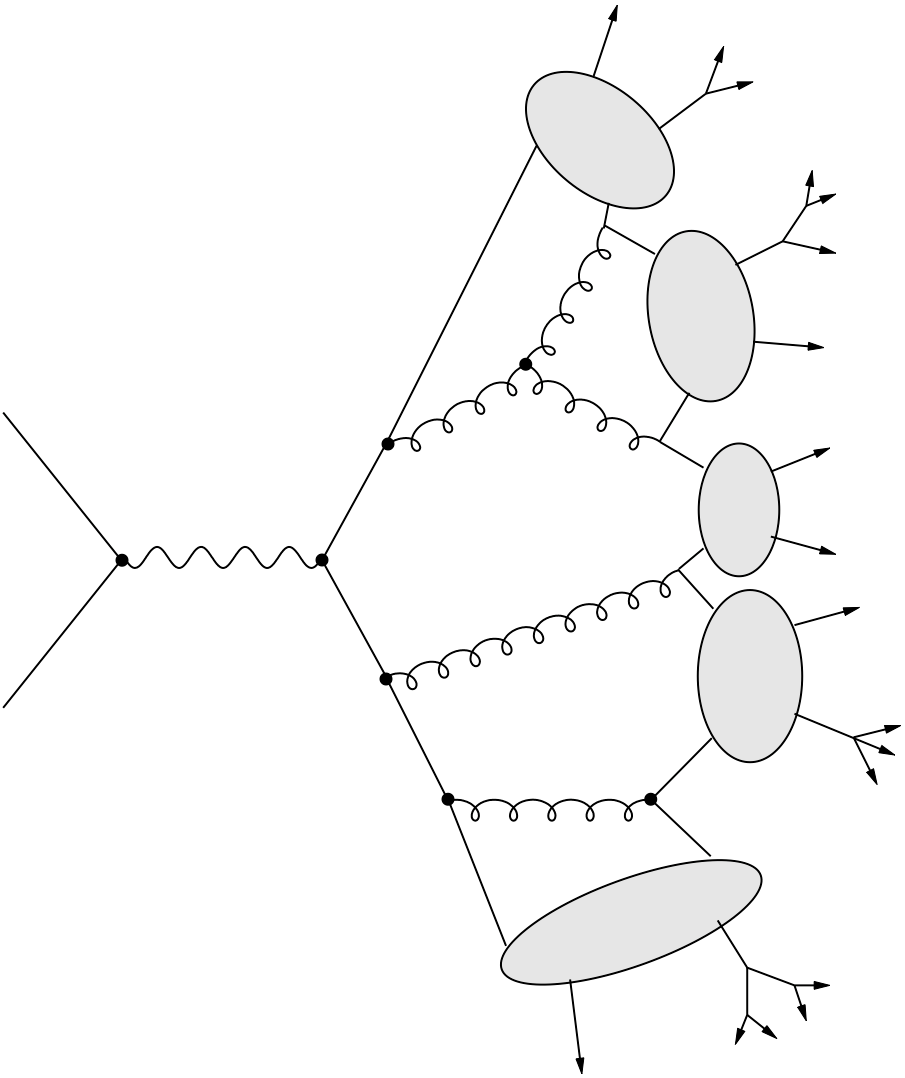
\includegraphics[width=0.35\textwidth]{figures/simul/Figures_MonteCarlo_clustr_had.pdf}
%    \label{fig:cluster_model}
%  }
%\end{center}
% chiara note: check reference!
 %\caption{Schematic view of \subref{fig:string_model} the string hadronization model and \subref{fig:cluster_model} the cluster hadronization model. 
% Figure from Ref. \cite{Isildak:2013kfa}.}
%  \label{fig:had_model}
%\end{figure}


These two hadronization models were developed in the 1980's, and since then there has been no fundamental progress in the theoretical understanding of hadronization. 
When the simulation of the events stops before hadronization, it is referred to as ``parton-level''.

\subsection{Underlying event}

The partons from the colliding protons that do not participate in the hard scattering can undergo interactions as well, giving origin to multiple parton interactions in the same collision (underlying event).
These secondary interactions are in general of lower momentum, since the \gls{me} is larger for low momentum transfer, and will contribute to the activity along the beam direction, less in the transverse plane. 
When the two protons pass through each other the likelihood of having multiple parton interactions depends on the overlap between the two protons. 
To model the underlying event, the assumption is made that these processes are $2\rightarrow2$ scattering; the \gls{me} for these diverges at small angle, so the modeling is dependent on the chosen \pt cutoff. 
Because of the low-\pt nature of the underlying event, its description is based on phenomenological models \cite{ATL-PHYS-PUB-2014-021,Skands:2010ak}.
To model the data, color reconnection between the primary interaction and the underlying event is needed. 

\subsection{Pileup}

The term pileup refers to additional \gls{pp} interactions taking place in the same bunch crossing (in-time pileup) or in events in different bunch crossings (out-of-time pileup). 
The presence of pileup challenges the reconstruction of the event, as it gives rise to extra activity overlapping with the products of the hard-scattering. The techniques used to model in-time pileup are the same as for the underlying event; 
for out-of-time pileup, similar methods are used but it is necessary to simulate the time response of the detector electronics to collisions from the previous bunch crossing. 

\section{Monte Carlo generators}
\label{sec:mcgen}

The simulations described in the above sections are carried out by event generators, that can be either general purpose, 
if they can reproduce all of the steps of the event generation, or specialized to one functionality. 
In this section the main characteristics of the generators used in the analyses described in this thesis are reviewed.

\subsection{General purpose generators}

Several independent software packages allow to study the effects of different modeling of the hadronization and different choices for the parton shower. The three main general-purpose event generators are:

\begin{description}
\item[\PY] \cite{Sjostrand:2006za,Sjostrand:2014zea} is a general purpose generator that uses \gls{lo} \glspl{me} for $2\rightarrow n $ ($n \leq 3$) processes; 
it is capable of simulating both hard and soft interactions, including \gls{isr} and \gls{fsr} and multiple parton interactions.
It uses a \pt-ordered parton shower and the Lund string hadronization model. It is commonly used as a \gls{psh} generator, interfaced with a different generator that computes the \glspl{me}.

\item[\HW] \cite{Corcella:2000bw,Bahr:2008pv,Bellm:2015jjp} has the same capabilities as \PY with few small differences. 
It computes $2\rightarrow 2$ \gls{lo} \glspl{me}.
 The partons shower is ordered by the angle of the emitted parton. Gluon splitting processes ($g \rightarrow q\bar{q}$ and $g \rightarrow gg$) in the collinear approximation are not symmetric in the azimuthal direction due to interference of positive and negative helicity states in the original gluon. 
While \PY uses a method that takes these affects into account only partially \cite{Webber:1987uy}, \HW uses one that fully includes spin correlations \cite{Collins:1987cp}. The hadronization is based on the cluster model.
\HW is typically interfaced with the standalone software \jimmy \cite{Butterworth:1996zw} that simulates the underlying event.

\item[\Sherpa] \cite{Gleisberg:2008ta} The \Sherpa event generator can provide multi-leg \glspl{me} both at \gls{lo} (up to four extra partons) and at \gls{nlo} (up to two extra partons). 
The matching between the \gls{me} and the dipole-type parton shower \cite{Schumann:2007mg} follows the CKKW prescription.
It uses a cluster hadronization model. 

\end{description}

The recent versions of all three generators are coded in C++, but \HW and \PY were originally developed in Fortran.  

\subsection{Matrix elements generators}

The generators described in this section do not provide a full description of the event, but aim instead at improving the 
computation of the \glspl{me}, and can be afterwards interfaced to a general purpose generator to simulate parton shower, underlying event and pileup. The most common \gls{me} generators are:

\begin{description}
\item[\PowhegBox] \cite{Alioli:2010xd} In this framework it is possible to implement \gls{nlo} \gls{me} computations, using the 5-flavor scheme.
It uses the \Powheg method for matching. 

\item[\aNLO] \cite{Alwall:2014hca} This generator can compute \glspl{me} at \gls{lo} for any user-specified Lagrangian, and at \gls{nlo} accuracy for selected processes. %It includes up to two additional partons and 
The \gls{nlo} calculation implements the \mcatnlo method. 
It is then interfaced to a parton shower using the 
MLM prescriptions at \gls{lo} and the FxFx prescription at \gls{nlo}.

\end{description}

\subsection{Specialized generators}

The specialized generators provide a better description of one specific aspect of the \gls{mc} simulation. Some of them are:

\begin{description}
\item[\evtgen] \cite{Lange:2001uf} This package simulates the decay of heavy flavor particles, in particular \textit{B} and $D$ hadrons. 
In the simulation of the decay it uses decay amplitudes instead of probabilities and it includes spin correlations. 
When interfaced with other event generators, it can be used to re-decay the heavy flavor particles, 
substituting original decay chains by the more sophisticated simulation by \evtgen.

\item[\tauola] \cite{Jadach:1990mz} General purpose event generators treat tau leptons as stable particles. 
The tau decays are then handled by separated packages like \tauola, which includes leptonic and semileptonic decays, paying attention to the tau polarization. Since the format of the tau-related information is generator-dependent and the results of the original generator need to be replaces, also the input and output formats of \tauola depend on the generator it is interfaced with.

\item[\photos] \cite{Barberio:1990ms} This generator handles electromagnetic radiation, estimating the size of the \gls{qed} bremsstrahlung in the collinear approximation, and is used e.g. by \tauola. 


\end{description}


\section{Detector simulation}
\label{sec:detsim}

The outcomes of the event simulation are the four-vectors of all the stable particles produced in the final state of the event, stored in the standard HepMC format \cite{Dobbs:2001ck}.
When this information is used directly, the analysis is referred to as ``particle level'' analysis; furthermore, if we want to filter the simulated events based on the final state, this can be done at this stage. 
While the event generation can already provide information on the kinematic of the event, it is not enough to compare the \gls{mc} simulations with the 
data collected by the \gls{atlas} detector. 
After the event simulation, the \gls{atlas} simulation chain \cite{Aad:2010ah} (described in Figure \ref{fig:sim:chain}) proceeds with the emulation of the
interaction of the particles with the detector and the signal generated in each of the detector's subsystems, 
which is done with the \geant package \cite{Agostinelli:2002hh}. The configuration of the detector, including any misalignment, can be set at run time, and the energy depositions are recorded as hits. The digitalization step takes the input hits from the hard scattering, underlying event and pileup and transforms them into detector signals, adding also detector noise. Also the response of the \gls{lone} trigger (described in Section \ref{sec:cern:trigger}) is simulated at this stage. The final output of the digitalization is the \gls{rdo} file, to which the output of the \gls{atlas} detector itself, which is in ``bytestream'' format, can be converted as well. The \gls{hlt} decision and the event reconstruction run on the \gls{rdo} data format. After the detector simulation, the \gls{mc} simulated events are treated in the same manner as data, going through the object reconstruction procedures
described in Chapter \ref{sec:event:reco}.

\begin{figure}[h]
\begin{center}
    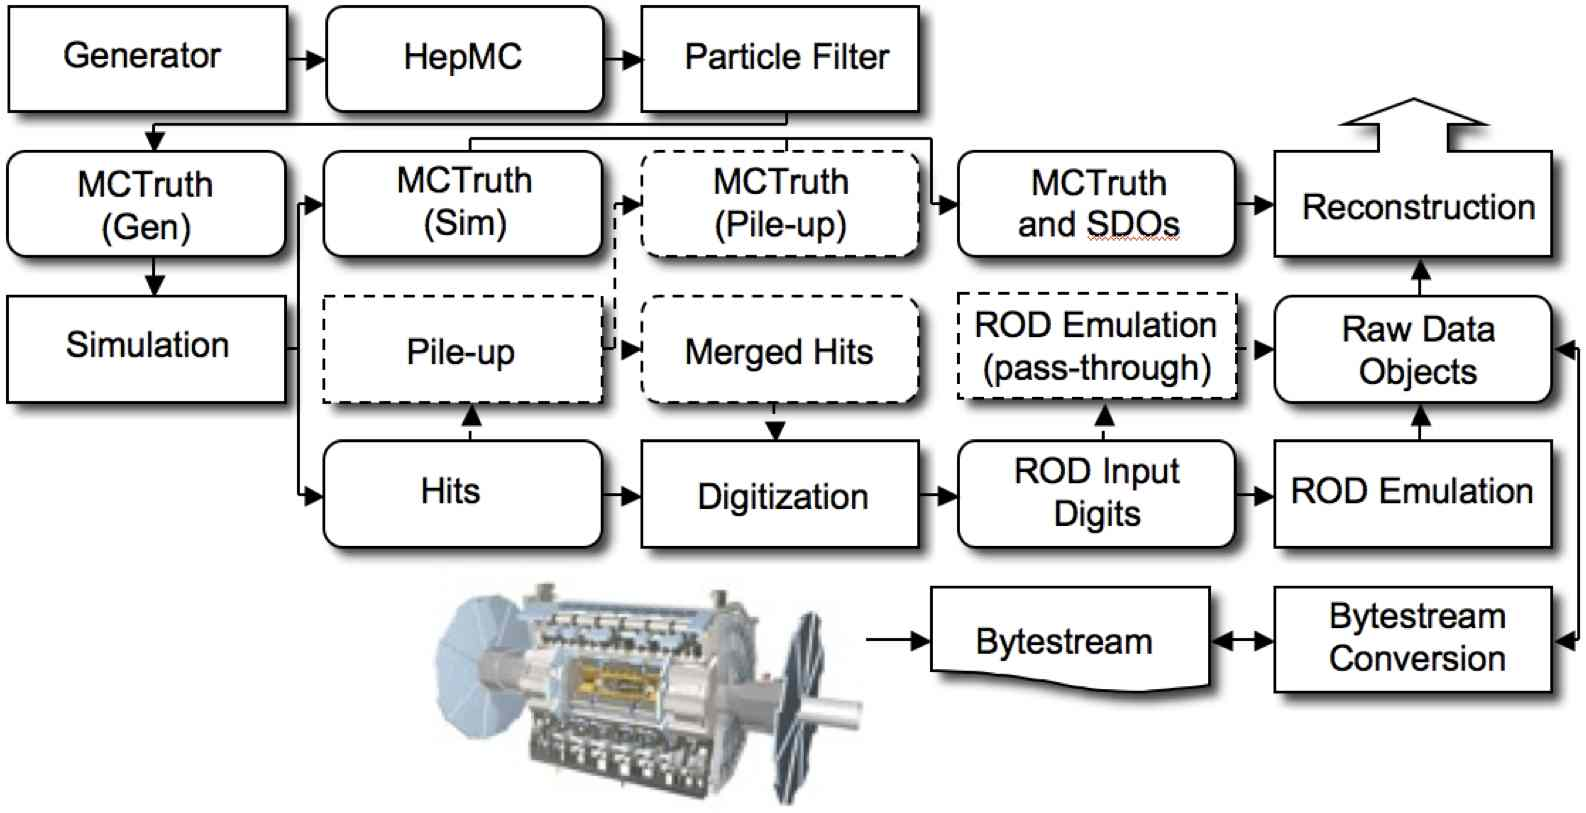
\includegraphics[width=0.8\textwidth]{figures/simul/outline_v2}
\end{center}
\caption{The \gls{atlas} simulation chain, compared with the processing of the recorded data; square-cornered boxes represent algorithms, while data objects are represented as rounded boxes. Figure from Ref. \cite{Aad:2010ah}.}
 \label{fig:sim:chain}
\end{figure}

The full simulation of the interaction of particles with the \gls{atlas} detector is a CPU-intensive task. 
ATLFAST-II \cite{Aad:2010ah} is a fast simulation method 
%aiming at simulating the large amount of \gls{mc} events required by \gls{atlas} analyses by 
making use of a simplified detector description. 
It has two components: the fast ATLAS tracking simulation (Fatras) \cite{Edmonds:2008zz}, to emulate the response of the \gls{id} and of the muon system, 
and the fast calorimeter simulation (FastCaloSim) \cite{ATL-PHYS-PUB-2010-013}, that takes care of the simulation of the calorimeters. The default ATLFAST-II simulation uses the full \geant simulation for the \gls{id} and the muon spectrometer, 
while it uses FastCaloSim to emulate the energy deposited in the calorimeters using a parametrization of the longitudinal and lateral energy profile. 
ATLFAST-IIF uses both FastCaloSim for the calorimeters and Fatras for the tracking systems. 
The output of ATLFAST-II includes all the properties necessary to run the same event reconstruction as with \geant or the real data.

%\section{Data-driven corrections}
%\label{sec:datacorr}

The simulated event samples are normalized to the highest-available-order cross-section, 
and events are reweighted so that the simulated pileup distribution matches that observed in the data.
Despite the accurate simulation, residual differences can be present in the reconstruction and selection efficiency in data and \gls{mc} simulation. 
The simulated reconstruction and selection efficiencies are corrected with multiplicative \glspl{sf}, defined as:
\begin{equation}
{\rm SF} = \frac{\epsilon_{\rm data}}{\epsilon_{\rm MC}} \; , \nonumber
\end{equation}
\noindent where $\epsilon_{\rm data}$ and $\epsilon_{\rm MC}$ are measured in dedicated data calibration samples 
and in the equivalent \gls{mc} simulation, respectively.
These \glspl{sf} can be function of the kinematic of the physics objects in the event (often \pt and $\eta$). 
Some examples of \glspl{sf} for the physics objects relevant for the analyses described in this thesis are provided in Chapter \ref{sec:event:reco}.
Analogously, energy scale and resolution of the different physics objects in the simulation are corrected 
to match the corresponding measurements in data.


\clearpage 
\bibliographystyle{atlasBibStyleWithTitle}
\addcontentsline{toc}{section}{Bibliography}
\bibliography{main}


%\glsresetall 
\glsunset{atlas}
\glsunset{cms}
\chapter{Event reconstruction}
\label{sec:event:reco}

The particles produced in the \gls{pp} collisions in the center of the \gls{atlas} detector interact with the detector material as discussed in Chapter \ref{chap:cern}. As a result of these interactions, electrical signals are recorded. Event reconstruction is the process of recombining these digital signals and interpreting them as tracks and energy deposits in the calorimeters. Finally, a particle identification step
is performed, where the information from the relevant subdetectors is combined to reconstruct as accurately
as possible a candidate physics object.
This chapter describes the reconstruction and identification of the objects used in the analyses discussed in this thesis: tracks and vertices, hadronic jets, muons, electrons and missing transverse momentum. 


\section{Tracks and primary vertices}
\label{sec:reco:tracks}

In \gls{atlas} the identification of tracks from charged particles relies on the information collected by the \gls{id}. The tracking information is crucial to the reconstruction and identification of many types of particles, including electrons, muons, and the jets originating from the hadronization of a \textit{b}-quark. 
Charged particles traversing the \gls{id} deposit energy through ionization,  
which is read out as hits; in the Pixel detector each hit corresponds to a space point, 
while in the \gls{sct} the space points are obtained as pairs of hits from each side of the modules. 
The space points are used to reconstruct the trajectory of the charged particles, which 
is helicoidal and with radius inversely 
proportional to their momentum, 
since the \gls{id} is surrounded by a solenoidal magnetic field.
The precision on the position measurement of the track depends on the granularity of the different subsystems of the \gls{id}.


After the point of closest approach (perigee) to a given reference is defined, the trajectory of the track can be described by five parameters: 
\begin{equation}
\theta, \; \phi, \; q/p, \; d_0, \; z_0 \;, \nonumber
\end{equation}
\noindent where $\theta$ and $\phi$ are the azimuthal and polar angle, $q/p$ is the ratio of the charge of the track to the track momentum, and $d_0$ and $z_0$ are the distance to the point of closest approach to the vertex in the transverse plane and along the $z$-axis. 


Primary tracks, originating from charged particles with a life time longer that $3 \times 10^{-11}$ s produced directly in the hard-scatttering vertex, are reconstructed with an inside-out approach \cite{Cornelissen:1020106}: the seed of the reconstruction are three hits in the silicon detector, and then compatible hits in the outer layers of the \gls{id} are added with a Kalman Filter \cite{citeulike:347166,Fruhwirth:1987fm}. The \gls{trt} segments that are not associated with primary tracks are used as starting point to reconstruct tracks from long-lived particles or from material interaction, with a back-tracking that extrapolates the \gls{trt} information to the pixel hits. 

Random groups of hits can be wrongly reconstructed as belonging to the helical trajectory of a track (fake tracks). The amount of fake tracks increases with the increase of pileup, and can be reduced by tightening the selection criteria of the track, at the expense of reconstruction efficiency. Three different selection criteria are used for the data collected in 2015 and 2016 (Loose, Loose-Primary and Tight-Primary), that differ in the requirements on the hits and holes (elements where a hit was expected but was not registered) in the different \gls{id} layers. The track reconstruction efficiency is measured in \gls{mc} simulations as the ratio of the reconstructed tracks matched to a generated charged particle over the total number of generated charged particles. The reconstruction efficiency as a function of the track $\eta$ and \pt is shown in Figure \ref{fig:obj:tracks} for Loose and Tight-Primary tracks.
 
\begin{figure}[ht]
\centering
\subfigure[]{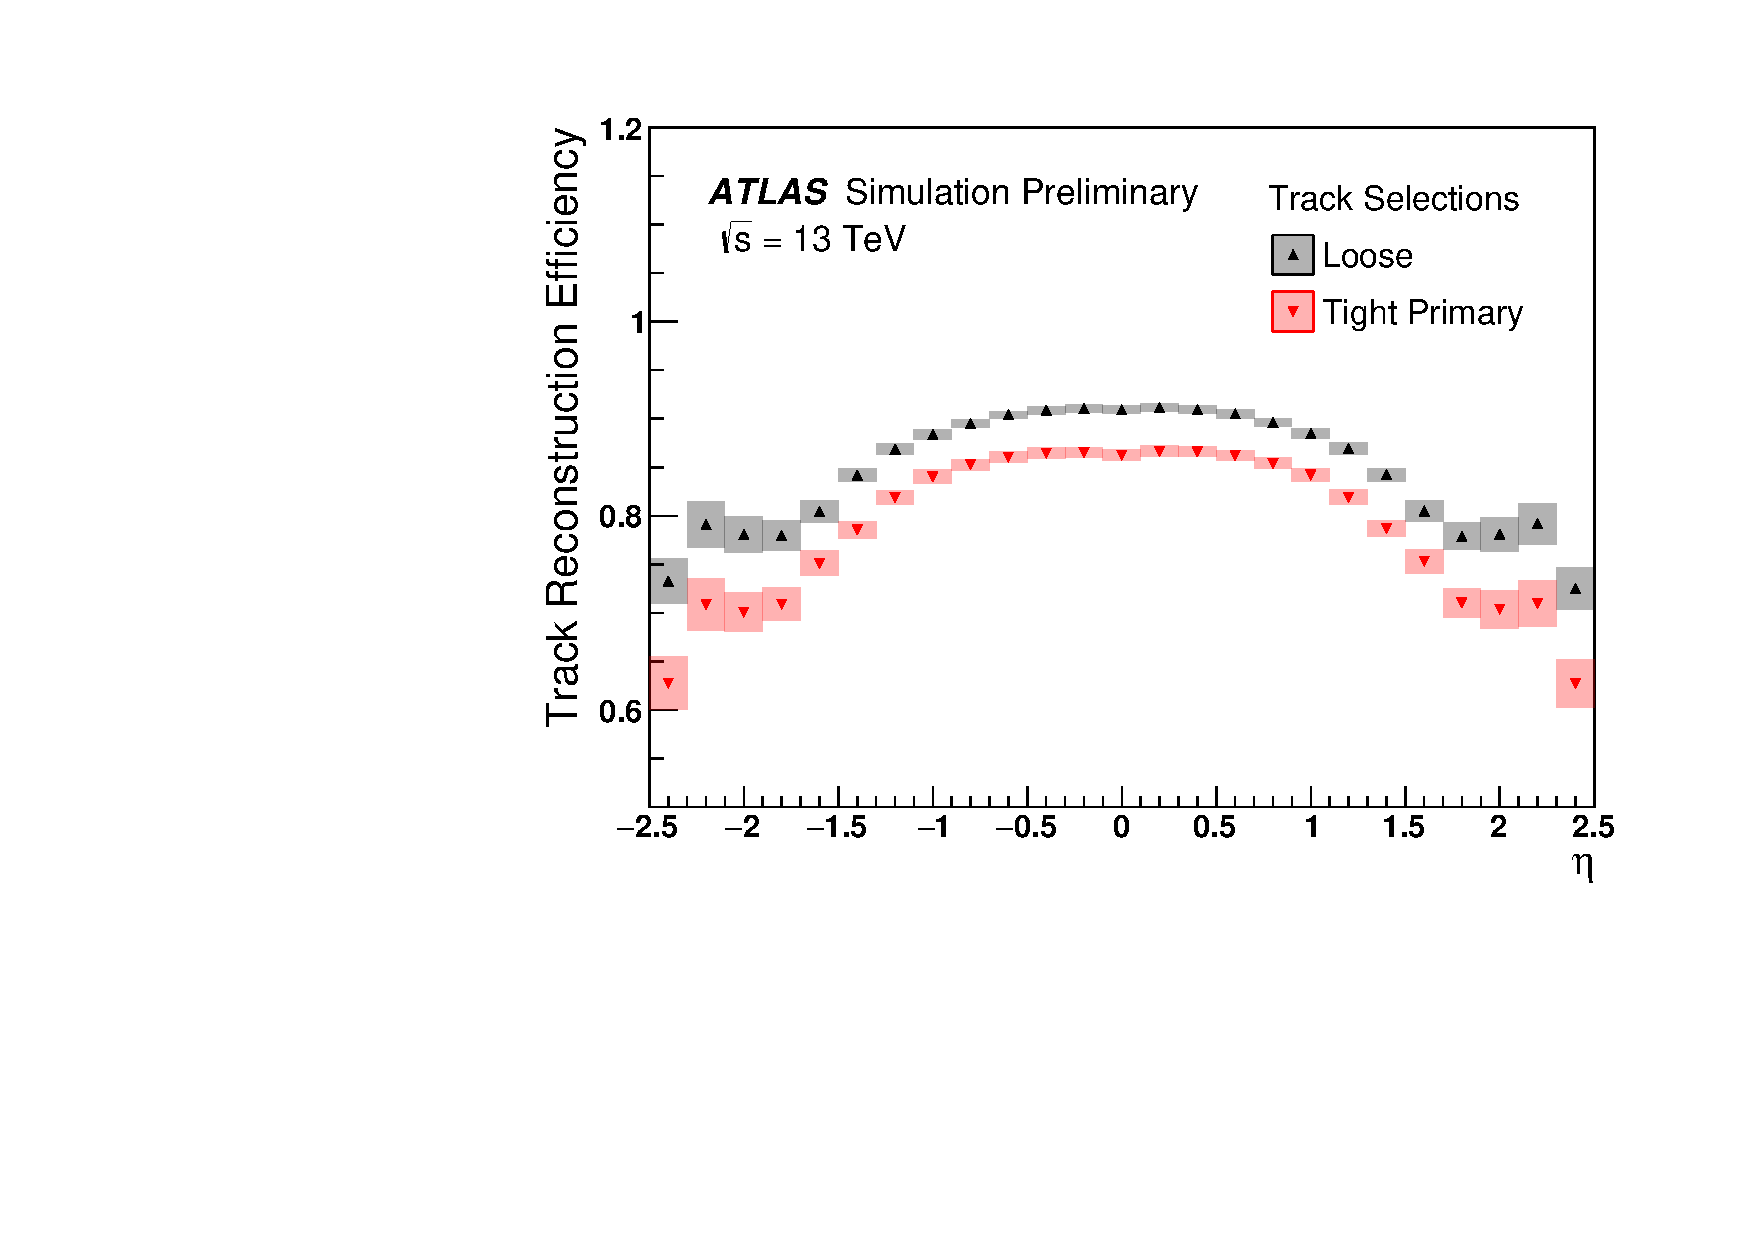
\includegraphics[width=0.48\textwidth]{figures/objects/track1}}
\subfigure[]{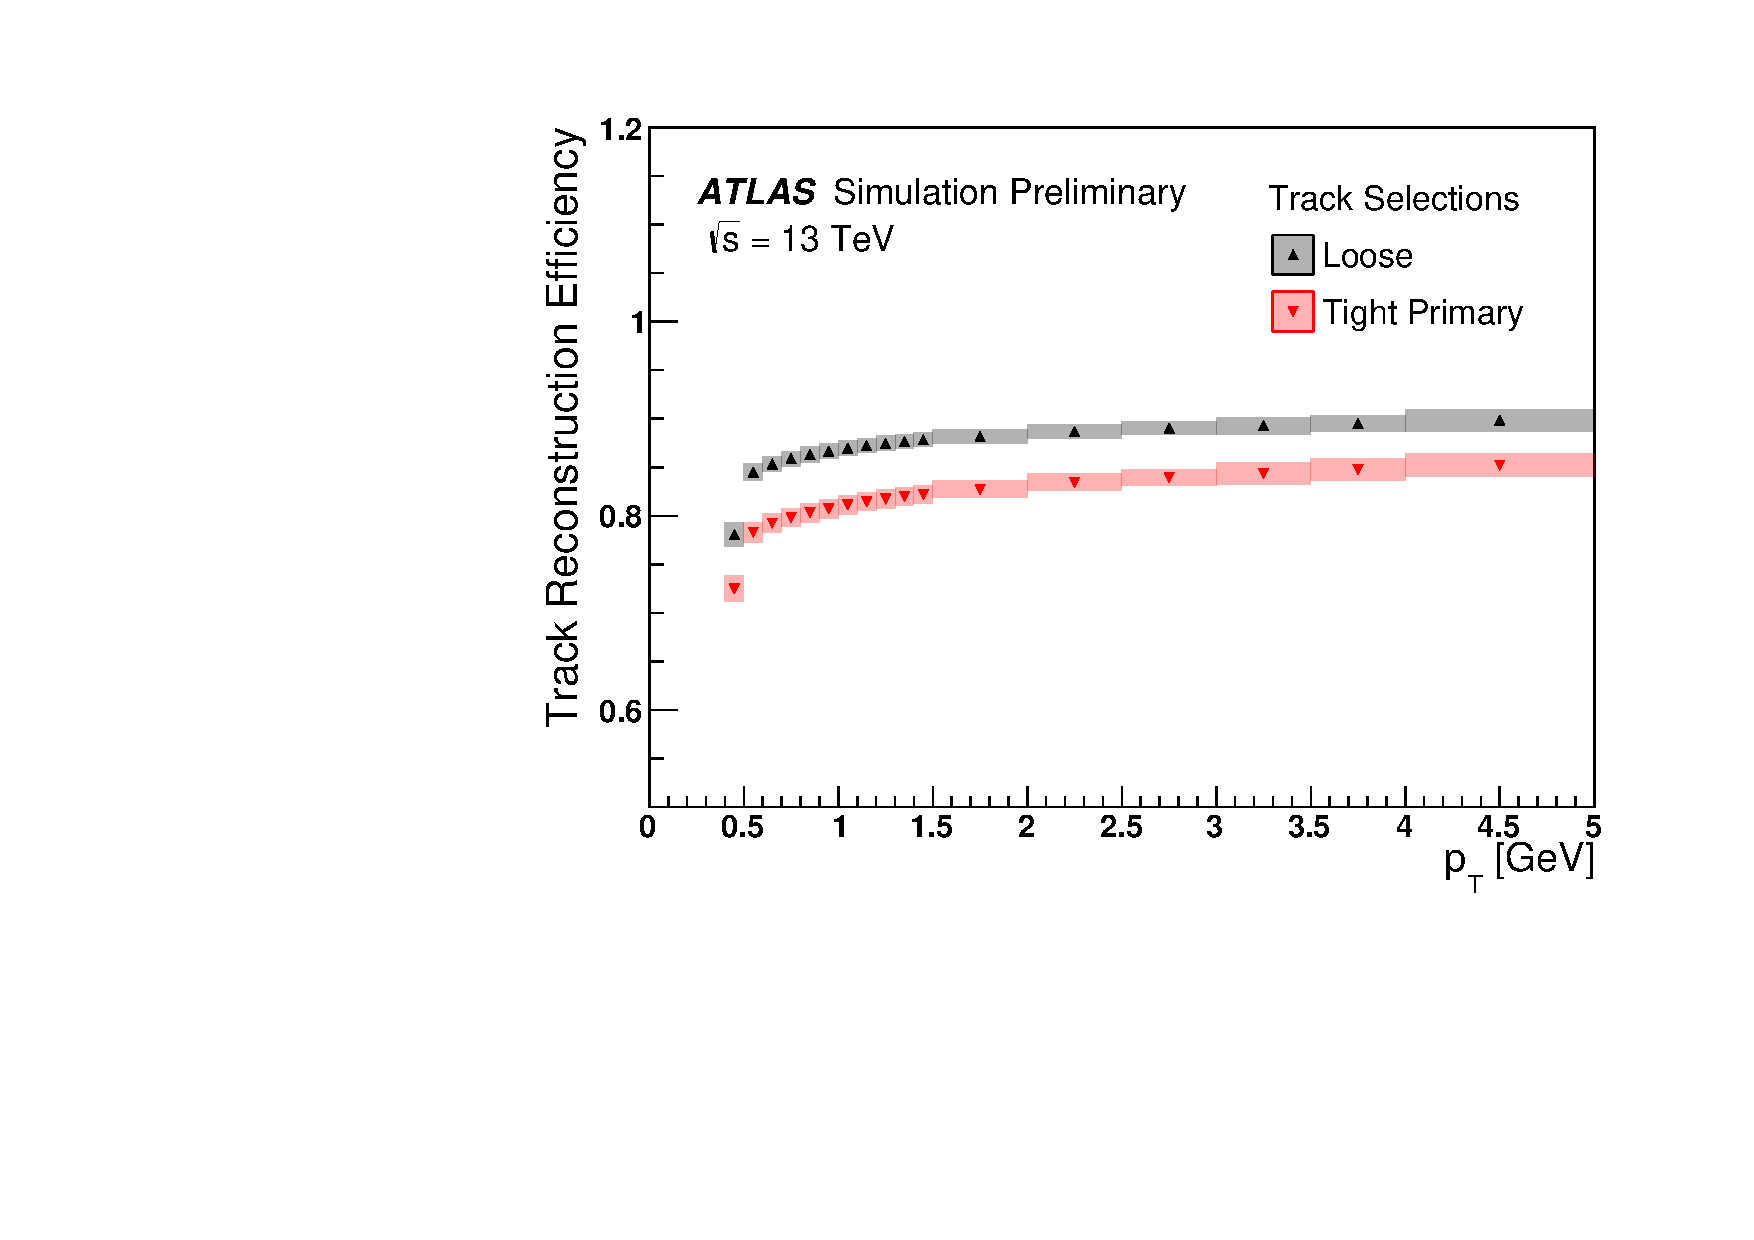
\includegraphics[width=0.48\textwidth]{figures/objects/track2}}
\caption{Track reconstruction efficiency, evaluated by using minimum bias simulated events, as a function of truth $\eta$ (a) and \pt (b) for Loose and Tight Primary track selections. The bands indicate the total systematic uncertainty. Figure from Ref. \cite{ATL-PHYS-PUB-2015-051}.}
\label{fig:obj:tracks}
\end{figure}

Tracks are the starting point for the identification of the interaction points, referred to as \glspl{pv}. 
\glspl{pv} are reconstructed through a vertex finding algorithm \cite{Fruhwirth:2007hz}, 
and then the vertex fitting algorithm identifies the vertex position and refits the tracks 
adding the constraint of the reconstructed interaction point. 
The \gls{lhc} operates in a high-luminosity regime, which makes it likely to have multiple \gls{pp} interactions per bunch crossing, 
and therefore multiple reconstructed \gls{pv} candidates. 
Once all the \gls{pv} candidates are reconstructed, the one with the highest sum of the squared transverse momenta of its associated tracks ($\sum_i^{N-tracks}p_{T,i}^2$) is identified as the hard scattering \gls{pv}, and the position of physics objects is recomputed with respect to its coordinates. The other vertices are named pileup vertices, and their number is correlated  to the number of interactions per bunch crossing.


\section{Jets}

Because of confinement, quarks and gluons produced in the collisions give origin to a collimated spray of hadrons (jets) that move in the direction of the original parton. When jets interact with the detector, they loose most of their energy as deposits in the calorimeter systems, which are then grouped together aiming at reconstructing the characteristics of the original parton. 

\subsection{Clusters}
The first step in the jet reconstruction is the procedure that groups the calorimeter cells in three dimensional objects referred to as topological clusters (topoclusters) \cite{ATL-LARG-PUB-2008-002,Aad:2016upy}. Topoclusters are built starting from seed cells with a signal-to-noise ratio higher than 4. All the neighboring cells with signal-to-noise ratio higher than two are added with an iterative procedure, and finally a ring of guard cells are added independently of their signal.  
Topoclusters are calibrated at the \gls{em} scale, which means that the proportionality constant between the readout current and the particle energy is correct only for particles of an \gls{em} shower.

\subsection{Jet-finding algorithms}
\label{sec:obj:jetfinding}

The topoclusters are then grouped together by a jet-finding algorithm. Different algorithms are available, and in particular the algorithms of the $k_T$-family merge clusters according to the metric $d_{i,j}$, defined as:

\begin{equation}
d_{i,j} = min\left( k_{T,i}^{2n}, k_{T,i}^{2n}  \right) \frac{\Delta R_{i,j}^2}{R^2} \; ,
\label{eq:obj:dij}
\end{equation}

\noindent where $k_{T,i}$ is the transverse momentum of the cluster, $\Delta R_{i,j}$ is the angular distance defined as in Equation \ref{eq:cern:dR}, 
$R$ is a fixed parameter, whose value sets the size of the jet, and $n$ is the parameters that defines the kind of algorithm we are using 
and therefore the shape of the resulting jets. 
Equation \ref{eq:obj:dij} defines the distance between two clusters, while the cluster-beam distance is defined as:

\begin{equation}
d_{i,B} =  k_{T,i}^{2n} \; . \nonumber
\end{equation}

The grouping of clusters follows an iterative approach:
\begin{enumerate}
\item For each topocluster, the distances $d_{i,j}$ and $d_{i,B}$ are calculated.
\item If, for some $i$ and $j$, $d_{i,j} < d_{i,B}$, the two clusters with the smallest $d_{i,j}$ are grouped. 
\item Otherwise, if $d_{i,B} < d_{i,j} \, \forall i \neq j $ the $i$-th cluster is defined as a jet.
\item This procedure is iterated until all inputs have been classified into jets.
\end{enumerate}

\noindent Depending on the value of the parameter n, we can distinguish different algorithms:
\begin{itemize}
\item $n=0$: Cambridge-Aachen. The grouping of the clusters depends only on geometrical considerations and not on their momentum. 
\item $n=1$: $k_T$ algorithm. Soft clusters are grouped first.
\item $n=-1$: anti-$k_T$ algorithm. Groups hard objects first; the shape of the jets is more regular than in the two previous cases and is a cone of radius R.
\end{itemize}

The choice of a particular algorithm results in different shapes of the jets, as discussed in Ref. \cite{cacciari:antikt}. 
The standard algorithm used by \gls{atlas} is the anti-$k_T$ algorithm, which leads to jets with a more regular shape 
in the ($\eta$-$\phi$) plane. 

\subsection{Jet calibration}
\label{sec:obj:jetcalib}

As mentioned previously, the inputs to the jet-finding algorithm are calibrated at the \gls{em} scale, and its coordinates refer to the center of the detector. To access a more precise measurement of the jet energy and kinematics, a sequence of calibration steps is applied; 
%for the 2015--2016 dataset, 
the standard \gls{atlas} corrections are \cite{PhysRevD.96.072002}:

\begin{description}
\item[Origin correction] The direction of the jet is changed to point to the reconstructed hard-scattering \gls{pv} rather than to the cented of the detector. This correction improves the $\eta$ resolution of the jets.

\item[Pileup correction] Multiple collisions in the same bunch crossing (in-time pileup), as well as residual energy from previous collisions (out-of-time pileup), affect the jet energy reconstruction. The effect of pileup is corrected in two steps 
\cite{Cacciari:2007fd,ATLAS-CONF-2013-083}: a first correction, dependent on the number of \glspl{pv}, uses the jet area to subtract form the jet energy the average energy form pileup events. 
The jet area is measured with ghost-association: simulated ghost particles of infinitesimal momentum are added to the event uniformly in solid angle prior to jet reconstruction, and the jet area is computed from the fraction of ghost particles associated to the jet after the clusters are merged. 
A second correction based on the number of \glspl{pv} and on the number of interactions per bunch crossing is then applied to disentangle the effect of in-time pileup and out-of-time pileup.

\item[Absolute calibration] The absolute \gls{jes} and $\eta$ correction is derived comparing in \gls{mc} the truth energy of a jet 
(defined as the energy of the truth jet with $\Delta R<0.3$ from the calorimeter jet) 
with the reconstructed energy, and it also corrects for biases in the $\eta$ reconstruction \cite{Aad2015jets}.

\item[Global sequential calibration] The \gls{gsc} \cite{ATLAS-CONF-2015-002} improves the \gls{jes} resolution by deriving additional corrections based on individual jet properties, e.g. the number of associated tracks and the fraction of energy deposited in the various layers of the calorimeter.

\item[In-situ calibration] As a last stage, the data-driven calibration (in-situ) \cite{ATLAS-CONF-2015-017} corrects for the differences between \gls{mc} simulation and data (arising e.g. from imperfect simulation of the detector response and material interaction). These corrections are derived from events where the jet \pt is balanced against other well measured objects. In the $\eta$-intercalibration, dijet events are used to correct the response of forward jets (with $0.8 < |\eta| < 4.5$) using well-measured central jets (with $|\eta| < 0.8$). 
The response of central jets is instead measured in $Z$+jets, $\gamma$+jets and multijet events; 
in $Z$/$\gamma$+jets events, the \pt of the jet is measured against the \pt of a well measured $Z$ boson or photon, while 
multijet events are used to calibrate central high-\pt jets ($300 < \pt < 2000$ GeV) against 
well calibrated low-\pt central jets. 
 
\end{description}

\subsubsection*{Jet calibration uncertainties}

The calibration procedure described above implies a set of uncertainties. In particular, 
the \gls{atlas} \gls{jes} Run-2 calibration includes a set of 80 systematic uncertainties; 
67 of those derive from the in-situ calibration \cite{PhysRevD.96.072002}, accounting for modeling uncertainties, 
sample statistical uncertainty and uncertainties in the calibration of other physics objects used in deriving the calibration. 
The other 13 systematic uncertainties derive from the pileup correction, the $\eta$-intercalibration 
and differences in the jet response and composition for jets of different flavors. 
The full combination of the uncertainties derived from the first 3.2 \ifb of the Run 2 data 
is shown in Figure \ref{fig:obj:jessyst} as a function of \pt at $\eta = 0$ and as a function of $\eta$ at \pt$ = 80$ GeV.

\begin{figure}[h]
\begin{center}
  \subfigure[]{
    \label{fig:Comb_syst:pt}
    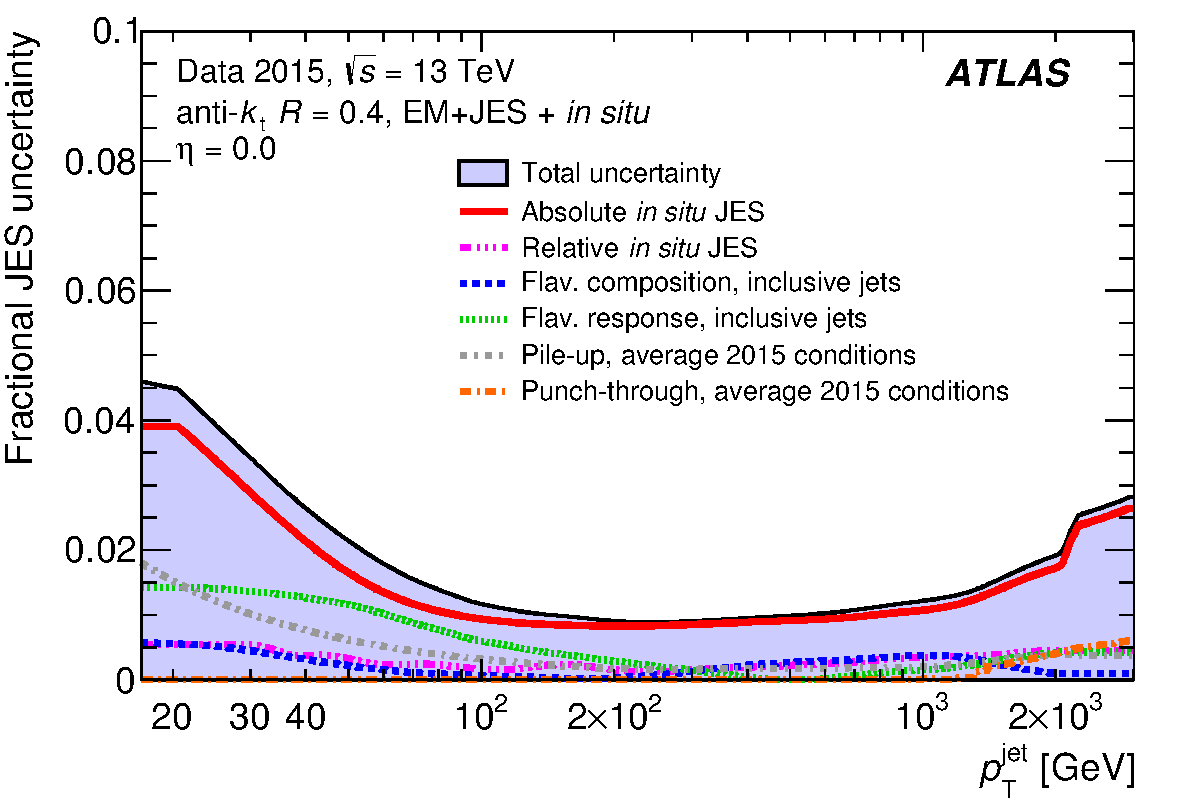
\includegraphics[width=0.48\textwidth]{figures/objects/fig12a.pdf}
  }
  \subfigure[]{
    \label{fig:Comb_syst:eta}
    \includegraphics[width=0.48\textwidth]{figures/objects/fig12b.pdf}
  }
\end{center}
 \caption{Combined uncertainty in the \gls{jes} of fully calibrated jets as a function of \subref{fig:Comb_syst:pt}  
 jet \pt at $\eta = 0$ and \subref{fig:Comb_syst:eta} $\eta$ at \pt$ = 80$ GeV. Figure from Ref. \cite{PhysRevD.96.072002}.}
  \label{fig:obj:jessyst}
\end{figure}

To allow an easier usage of the uncertainties in physics analyses, a reduced set of 19 \gls{np} is provided: 
the 67 \glspl{np} from the in-situ calibration are reduced to six by keeping the five uncertainties of largest magnitude, 
plus a sixth one which is the sum in quadrature of the remaining ones. 
A further reduction is in place to group the remaining \glspl{np} into three components, 
and the \glspl{np} within a single component are added in quadrature; this leads to a correlation loss, whose effect is analysis dependent. 

Jets with the same true energy can have different reconstructed energies; the distribution of the difference between true and reconstructed energy of a jet is modeled with a Gaussian, whose width is defined as \gls{jer}. The measurements for the in-situ calibrations can be used also to access the differences in \gls{jer} between data and \gls{mc} \cite{ATLAS-CONF-2015-057,ATLAS-CONF-2015-017}, and result into an additional \gls{np}.

\subsection{Jet vertex tagger}
\label{sec:jvt}

%It has already been discussed in Section \ref{sec:obj:jetcalib} how pileup is taken into account in the calibration of the \gls{jes}. 
Beside affecting the jet energy, high levels of pileup can also lead to the reconstruction of spurious jets not originating from the hard-scattering interaction. In \gls{atlas} track-based algorithms are used for the identification of pileup jets \cite{Aad:2015ina,ATLAS-CONF-2014-018}. 
Tracks are matched to calorimeter jets by ghost-association \cite{Soyez:2012hv}. Once the hard-scattering \gls{pv} (\gls{pv}$_0$) is identified, 
for each jet it is possible to compute the \gls{jvf}, the ratio of the scalar sum of the \pt of the tracks associated to the jet and originating from  \gls{pv}$_0$ to that of all the associated tracks:

\begin{equation}
 \JVF = \frac{\sum_m{p_{{\rm T}, m}^{{\rm track}}({\rm PV}_0)}}{\sum_n\sum_l  p_{{\rm T}, l}^{{\rm track}}({\rm PV}_n)} \; .
 \label{eq:jvf}
\end{equation} 

\noindent In this definition the index $n$ runs over all the vertices of the event. In high-pileup conditions the denominator in 
Equation \ref{eq:jvf} increases; to correct for this dependence, the \gls{cjvf} is introduced. 
This is a modified version of \gls{jvf}, that takes into account the dependence on the number of pileup tracks (\nPUtrk):

\begin{equation}
\cJVF = \frac{\sum_m{p_{{\rm T}, m}^{{\rm track}}({\rm PV}_0)}}{\sum_l p_{{\rm T}, l}^{{\rm track}}({\rm PV}_0) + \frac{\sum_{n\geq1}\sum_l p_{{\rm T}, l}^{{\rm track}}({\rm PV}_n)}{ (k \cdot \nPUtrk)}} \; , \nonumber
\end{equation}

\noindent with $k=0.001$. Another variable used to discriminate hard-scattering jets against pileup jets is the ratio of the scalar
sum of the \pt of the tracks originating from \gls{pv}$_0$ to the jet transverse momentum:


\begin{equation}
\RpT = \frac{\sum_k{p_{\rm{T}, k}^{{\rm track}}({\rm PV}_0)}}{\ptjet} \;.
\label{eq:obj:rpt}
\end{equation}

The \cJVF and \RpT variables are combined in a two-dimensional likelihood that constitutes a single tagger, the \gls{jvt}. 
The distribution of \gls{jvt} for hard-scattering and pileup jets in \gls{mc} simulation is shown in Figure \ref{fig:obj:jvt_mc},
while Figure \ref{fig:obj:jvt_data} shows the comparison of the \gls{jvt} distribution in data and \gls{mc} in a dimuon selection.


\begin{figure}[h]
\begin{center}
  \subfigure[]{
    \label{fig:obj:jvt_mc}
    \includegraphics[width=0.45\textwidth]{figures/objects/jvt.pdf}
  }
  \subfigure[]{
    \label{fig:obj:jvt_data}
    \includegraphics[width=0.51\textwidth]{figures/objects/jvt_data.png}
  }
\end{center}
 \caption{\subref{fig:obj:jvt_mc} Distribution of \gls{jvt} for pileup and hard-scatter jets with $20 < \pt < 30$ GeV. Figure from Ref. \cite{ATLAS-CONF-2014-018}. \subref{fig:obj:jvt_data} The JVT distribution, in Powheg+Pythia8 MC and in 2015+2016 data, of jets balanced against $Z$ bosons decaying to muons. Figure from Ref. \cite{jvtpublicplots}.}
  \label{fig:obj:jvt}
\end{figure}

\subsection{Jet cleaning}
\label{sec:jetcleaning}

Beside pileup jets, other spurious jets come from the non-collision background; this type of background includes muons originating from secondary cascades from beam losses, in which case we speak of beam-induced background, and from cosmic rays. These muons leave energy deposits in the calorimeters while traversing the detector, which can be interpreted as jets. Also coherent noise from the calorimeters can give rise to fake jets. In \gls{atlas} a set of quality criteria are designed to reject jets not originating from \gls{pp} collisions \cite{ATLAS-CONF-2015-029}. These quality criteria are rely on variables based on:
\begin{itemize}
\item Ionization signal shape in the LAr calorimeters, to remove mainly fake jets from calorimeter noise. 
\item Ratios of energies, e.g. the ratio of the energy deposited in the electromagnetic calorimeter to the total energy, or the ratio of energy in different calorimeter layers, that can be used to discriminate against jets from beam-induced background or calorimeter noise.
\item Tracks associated with the jets, and in particular variables similar to \RpT defined in Equation \ref{eq:obj:rpt}, that have in general lower value for fake jets than for jets originating from \gls{pp} collisions. 
\end{itemize} 

Different thresholds for the selections on these variable distinguish the two working points, \textit{BadLoose} and \textit{BadTight}, which have an efficiency respectively of 99.5\% and 95\% for jets with $\pt > 20$ GeV, while for jets with $\pt > 100$ GeV the efficiency of the two working points increases to 99.9\% and 99.5\%. The \gls{op} used in the searches discussed in Chapters \ref{chap:strong_prod} and \ref{chap:ewk_prod} is \textit{BadLoose}. 

\subsection{Re-clustered jets}
\label{sec:reclustering}

The angular separation between the decay products of a particle with mass $m$ and transverse momentum 
$p_T$ scales as:
\begin{equation}
\Delta R \approx \frac{2 m}{p_T} \; . \nonumber
\end{equation}

This indicates that the ideal value of the $R$ parameter described in Section \ref{sec:obj:jetfinding} can vary depending on the event topology that we want to capture. 
For example, the decay products of a heavy particle with a transverse momentum much larger than its rest mass (boosted object) could be better described by a 
single jet with a larger $R$ than with multiple jets with the ``standard'' 0.4 radius, 
as it happens e.g. in the decay of very energetic top quarks, $W$, $Z$ or Higgs bosons produced at the LHC.
Each different value of the $R$ parameter requires a dedicated calibration following the steps described in Section \ref{sec:obj:jetcalib}. 
Therefore, it is not always possible to choose the optimal value of the jet radius. 
A possible solution to this problem comes from noticing that the same jet-finding algorithms used to group topoclusters can have different types of inputs. 
In particular, jets themselves can be be used as input and grouped together, and in this case we speak of re-clustered jets \cite{Nachman:2014kla}. 
Re-clustered jets are automatically calibrated as long as the input jets are, and also the jet uncertainties can be propagated directly. 
A comparison of the jet clustering obtained with anti-$k_T$ $R$=1.0 and by re-clustering anti-$k_T$ $R$=0.3 jets into anti-$k_T$ $R$=1.0 jets 
is shown in Figure \ref{fig:recluster}. It is possible to see how the jet axis is similar between the two cases. 
Re-clustered jets can be trimmed by removing the constituent small-R jets that have a \pt smaller than a defined fraction of the \pt of the original reclustered jet. 


\begin{figure}[h]
\begin{center}
\includegraphics[width=0.8\textwidth]{./figures/springer/300571_37319012.pdf}
\end{center}
\caption{Example event where jets have been clustered with anti-$k_T$ with $R$=0.4 (red dots) and anti-$k_T$ $R$=1.0 (blue dots), and re-clustered starting from anti-$k_T$ $R$=0.4 jets (green stars); 
circles of radius 0.4 and 1.0 are drawn centred around anti-$k_T$ jets with $R$=0.4 and $R$=1.0 respectively. }
\label{fig:recluster}
\end{figure}

\section{Jets from B-hadrons}
\label{sec:btagging}

Jets originating from the hadronization of a \textit{b}-quark (\textit{b}-jets) can be identified thanks to the lifetime of \textit{B}-hadrons (about $10^{-12}$ s), which is shorter than the typical lifetime of hadrons containing only light quarks, but still long enough to allow the \textit{B}-hadrons to travel distances of the order of the mm before decaying. A schematic view of the topology originating from a jet containing a \textit{B}-hadron is shown in Figure \ref{fig:btag}. 

\begin{figure}[h]
\begin{center}
\includegraphics[width=0.75\textwidth]{./figures/springer/bjets.pdf}
\end{center}
\caption[Schematic view of the topology of a \textit{b}-jet.]{Schematic view of the topology of a \textit{b}-jet.}
\label{fig:btag}
\end{figure}

The procedure of identifying \textit{b}-jets is referred to as \textit{b}-tagging, and in \gls{atlas} is performed using as input the tracks associated to the jets. As already mentioned in Section \ref{sec:atlas:pixel}, between Run 1 and Run 2 a fourth pixel layer, the \gls{ibl}, was added to the \gls{atlas} detector, allowing a better impact parameter resolution and therefore improving substantially the \textit{b}-tagging performance. 

There are three families of \textit{b}-tagging algorithms that can be combined through multivariate techniques. The basic algorithms can be based on:

\begin{description}

\item[Impact Parameter] The transverse impact parameter of a track (\dzero) is the point of closest approach to the 
\gls{pv} in the transverse plane, while the longitudinal impact parameter (\zzerost) is defined as the distance along 
the $z$-axis between the \gls{pv} and the point of closest approach in the transverse plane. Because of the typical 
lifetime of \textit{B}-hadrons, on average \textit{b}-jets contain tracks with higher impact parameter than light-jets. 
The sign of the impact parameter is positive if the track extrapolation crosses the jet direction in front of the primary vertex, and negative otherwise. 
The negative side of the impact-parameter distribution derives from the 
impact-parameter resolution, and can be used to calibrate light-jets. In \gls{atlas}, two taggers make use of the information on the impact parameter
 \cite{ATLAS-CONF-2011-102}: IP2D, which is based on the significance of the transverse impact parameter (\dzero/$\sigma_{\dzero}$), and IP3D, which builds a two-dimensional template including also the significance of the longitudinal impact parameter (\zzerost/$\sigma_{\zzerost}$). The \gls{pdf} for each flavor hypothesis (\textit{b}, \textit{c}, and light) is derived from \gls{mc} simulation on a per-track basis, and then a \gls{llr} of the different probabilities is computed, including the contribution from all tracks associated to the jet. For example, the \gls{llr} discriminating \textit{b}-jets from light-jets is of the form $\sum_{i=1}^{N}\log\frac{p_b}{p_{light}}$, where the index $N$ runs on all the tracks associated to the jet. 

\item[Secondary Vertex Finding] The SV1 algorithm \cite{ATLAS-CONF-2011-102} explicitly looks for a secondary vertex within a jet. 
All the track pairs in the jet are tested for a two-track vertex hypothesis, removing the pairs that are likely to originate from 
long-lived particles (e.g. K$_0$, $\Lambda$), photon conversion or hadronic interaction with the detector material. 
If a two-track vertex remains, a new single vertex is fitted with the tracks passing this selection. 
\textit{B}-tagged jets are identified by high values of a likelihood discriminant, 
built using several variables 
including the decay-length significance, the invariant mass of all tracks associated with the vertex, 
the ratio of the sum of the energies of the tracks in the vertex to the sum of the energies of all tracks in the jet, 
and the number of two-track vertices.

\item[Identification of the Decay Chain] The \textit{B}-hadrons inside \textit{b}-jets decay with an electroweak interaction, 
through which a \textit{b}-quark decays preferentially to a \textit{c}-quark, since the \gls{ckm} matrix element $|V_{cb}|^2$ is much larger than $|V_{ub}|^2$. Hadrons containing a \textit{c}-quark ($D$-hadrons) subsequently decay as well, giving rise to a topology with two decay vertices. While the resolution is often not enough to reconstruct the two vertices individually, the JetFitter algorithm \cite{1742-6596-119-3-032032} operates assuming that they both lie on the same line, the flight axis of the \textit{B}-hadron. The information on the event topology derived with JetFitter is then used in a likelihood function, from which three different templates (one for each flavor) are derived.

\end{description}

The default \textit{b}-tagging algorithm used by \gls{atlas} in the analysis of the 2015--2016 dataset is MV2c10 
\cite{ATL-PHYS-PUB-2015-022,ATL-PHYS-PUB-2016-012}, 
a multivariate algorithm based on a \gls{bdt} that combines the algorithms described above. 
MV2c10 belongs to the family of MV2 algorithms, which are trained on a \ttbar sample using \textit{b}-jets as signal and \textit{c}-jets and light-jets as background, and differ in the relative fraction of \textit{c}-jets and light-jets that are
used in the training; in the case of MV2c10, the background sample in the training contains 15\% of \textit{c}-jets.
Figure \ref{fig:obj:mv2} shows the light-jet and \textit{c}-jet rejection as a function of \textit{b}-jet efficiency for different MV2 algorithms.

\begin{figure}[h]
\begin{center}
  \subfigure[]{
    \label{fig:obj:mv2_a}
    \includegraphics[width=0.48\textwidth]{figures/objects/mv2c10_a.pdf}  }
  \subfigure[]{
    \label{fig:obj:mv2_b}
    \includegraphics[width=0.48\textwidth]{figures/objects/mv2c10_b.pdf} }
\end{center}
 \caption{Light-jet \subref{fig:obj:mv2_a} and \textit{c}-jet \subref{fig:obj:mv2_b} rejection as a function of the \textit{b}-jet efficiency for the MV2 algorithms. Figures from Ref. \cite{ATL-PHYS-PUB-2016-012}.}
  \label{fig:obj:mv2}
\end{figure}

\glspl{op} are defined by a selection on the value of the \gls{bdt} output, and are designed to have a specific \textit{b}-jet efficiency.
Table \ref{tab:obj:mv2op} shows the \glspl{op} defined for the MV2c10 algorithm.

\begin{table}[h]
\begin{center}
    \includegraphics[width=1.0\textwidth]{figures/objects/btag_op.pdf}  
\end{center}
 \caption{Operating points for the MV2c10 \textit{b}-tagging algorithm. The efficiency and rejection rates are computed for jets with $\pt > 20$ GeV from \ttbar events. Table from Ref. \cite{ATL-PHYS-PUB-2016-012}.}
  \label{tab:obj:mv2op}
\end{table}

\subsection{B-tagging calibration and uncertainties}
\label{sec:obj:btaggingcalib}

The \textit{b}-tagging efficiency can be different in \gls{mc} simulation and data. The \textit{b}-tagging efficiency, 
\textit{c}-tagging efficiency and light mistag rate are measured in data for the \glspl{op} of Table \ref{tab:obj:mv2op}, 
and the \gls{mc} simulation is corrected with the \glspl{sf} derived as the ratio of the efficiency in data and in \gls{mc}. 
The \glspl{sf} are derived on a per-jet basis in a parametric form based on jet \pt, $\eta$ and truth flavor. 
For each \gls{mc} simulated event, an event-level \gls{sf} is derived by multiplying all the efficiency \glspl{sf} for the \textit{b}-tagged jets 
and all the inefficiency \glspl{sf} for the jets that are not \textit{b}-tagged. Several techniques are used in \gls{atlas} to measure the \textit{b}-tagging 
efficiency for the different jet flavors \cite{1748-0221-11-04-P04008}.
The calibrations used in the analyses described in this thesis are:

\begin{description}

\item[\textit{b}-jets] The default \textit{b}-tagging calibration for \textit{b}-jets is based on a \ttbar dileptonic sample. Events with exactly two opposite-sign leptons
and two or three jets are selected, and a per-event likelihood is built containing the \textit{b}-tagging weight \gls{pdf} for a jet of a given flavor;
the \gls{pdf} for light-jets and \textit{c}-jets is taken from \gls{mc}, while the \gls{pdf} for \textit{b}-jets is the information that we want to extract from data.
This last \gls{pdf} is described by a histogram with only two bins, one below and one above the threshold to \textit{b}-tag a jet. 

%\gls{bdt} based on 8 input variables 
%Likelihood fit using per-jet flavor correlations. 

\item[\textit{c}-jets] The analysis described in Chapter \ref{chap:strong_prod} uses a \textit{c}-jet calibration based on events where a $W$ boson 
is produced in association with a \textit{c}-quark. The events selected are the ones where the $W$ boson decays to an electron and a neutrino,
and the D-hadron originating from the fragmentation of the \textit{c}-quark decays to a muon. 
In $W+c$ production the electron and the muon in the final state have opposite charge, 
while most of the background processes have an equal number of same-sign and opposite-sign events. The number of $W+c$ events can therefore 
be obtained as the difference of these two categories.
For the higgsino search described in Chapter \ref{chap:ewk_prod}, which was developed at a later time, a new calibration for \textit{c}-jets, 
based on \ttbar events \cite{ATLAS-CONF-2018-001}, was available. 
This calibration selects \ttbar events where one of the $W$ bosons decays leptonically and the other one decays to a \textit{c}-quark and an s-quark. 

\item[light-jets] The \textit{b}-tagging efficiency of light-jets (mistag rate) is measured on an inclusive sample of jets, using the negative tag method 
\cite{ATLAS-CONF-2018-006}. 
The two main reasons that lead to \textit{b}-tagged light-jets are the finite resolution of the impact parameter and the secondary vertices caused
by long-lived particles and material interactions. If we consider only the first type of mistags, the signed impact parameter distribution 
will be symmetric around zero. 
The negative tag method is based on a modified version of the \textit{b}-tagging algorithms, that takes as input impact parameters and decay lengths with
reversed sign. The mistag rate is measured as the negative-tag efficiency of the jet sample, with \gls{mc}-based correction factors that take into account 
the negative-tag rate for \textit{b}- and \textit{c}-jets and the effect of long-lived particles and material interactions.

\end{description}

The \textit{b}-tagging scale factors are affected by multiple sources of uncertainty, which are reflected in uncertainties in the \glspl{sf}.
As an example, Figure \ref{fig:obj:btagSF} shows the \textit{b}-tagging \gls{sf} for \textit{c}-jets derived with the \ttbar calibration 77\% \gls{op}, 
and Figure \ref{fig:obj:mistagSF} shows the \glspl{sf} for light-jets derived with the negative tag calibration for the same \gls{op}.

%\note{Plots for other calibrations will be added after CONF are public (should be LHCP)}.

\begin{figure}[htbp]
\begin{center}
  %\subfigure[]{
  %  \label{fig:obj:ttSF}
    \includegraphics[width=0.48\textwidth]{figures/objects/cjettt_77SF.png}  %}
  %\subfigure[]{
   % \label{fig:obj:mv2_b}
    %\includegraphics[width=0.48\textwidth]{figures/objects/mv2c10_b.pdf} }
\end{center}
 \caption{\textit{B}-tagging \gls{sf} for \textit{c}-jets for the \gls{op} corresponding to the 77\% \gls{op}. Figure from Ref. \cite{ATLAS-CONF-2018-001}.}
  \label{fig:obj:btagSF}
\end{figure}

\begin{figure}[htbp]
\begin{center}
  \subfigure[]{
    \label{fig:obj:mistag1}
    \includegraphics[width=0.48\textwidth]{figures/objects/mistag_fig_05c.png}  }
  \subfigure[]{
    \label{fig:obj:mistag2}
    \includegraphics[width=0.48\textwidth]{figures/objects/mistag_fig_05d.png} }
\end{center}
 \caption{\textit{B}-tagging \gls{sf} for light-jets for the \gls{op} corresponding to the 77\% \gls{op} for \subref{fig:obj:mistag1} 
 $|\eta|<1.2$ and \subref{fig:obj:mistag2} $1.2 < |\eta| < 2.5$. Figures from Ref. \cite{ATLAS-CONF-2018-006}.}
  \label{fig:obj:mistagSF}
\end{figure}


\section{Muons}

Muon reconstruction and identification \cite{Aad:2016jkr} is based on the information collected by the \gls{id}, where muons are reconstructed as charged tracks, and by the \gls{ms}. 

\subsection{Muon reconstruction}

Both the \gls{id} and the \gls{ms} perform the reconstruction
of muon candidates independently and then the information is combined to build the muon candidates used in physics analyses. 
The reconstruction of muon tracks in the \gls{id} proceeds as described in Section \ref{sec:reco:tracks}. In the \gls{ms}, the first step is the identification of segments starting from the hits in each chamber. A muon track is reconstructed with a segment-seeded search (considering first the segments in the central layers of the detector as seeds, and then extending to the inner and outer ones). Except from the transition region between the barrel and the end-cap, tracks are required to have at least two matching segments; the hits associated to each track are fitted with a global \chis, and the track candidate is accepted or rejected based on the \chis value. 

Reconstructed muons can belong to four different types, depending on the subdetectors that contribute to their reconstruction:

\begin{description}
\item [Combined] Combined muons are built from a global fit that uses hits from tracks reconstructed independently in the \gls{id} and \gls{ms}.
\item[Segment-tagged] Muons of lower \pt or that cross regions of lower acceptance of the \gls{ms} can result in a segment in only one \gls{ms} chamber. If a track from the \gls{id} is associated with this segment, this track is classified as a segment-tagged muon.
\item[Calorimeter-tagged] A track in the \gls{id} is identified as a calorimeter-tagged muon if it is matched to an energy deposit in the calorimeter compatible with a minimum-ionizing particle. This muon category recovers identification efficiency for the muons that fall out of the \gls{ms} acceptance.
\item[Extrapolated] Extrapolated muons are reconstructed from tracks in the \gls{ms} compatible with originating from the \gls{ip}, to recover muons in high-$\eta$ regions, outside of the \gls{id} acceptance.
\end{description}

When multiple types of muon are reconstructed for the same physical object, the redundant ones are removed with an \gls{or} procedure that, when muons share the same \gls{id} tracks, gives priority to combined muons, and then to segment-tagged muons over combined muons. The \gls{or} with extrapolated muons gives preference to the \gls{ms} track with the best quality.

\subsection{Muon identification}
\label{sec:muon_id}

The reconstructed muons have to fulfill identification criteria that help reject the background constituted mostly by decays of pions and kaons. 
The variables used in the identification are the significance of the difference of the charge-over-momentum ratios measured by the \gls{id} and by the \gls{ms} ($q/p$ significance),
the difference of the \pt measured in the \gls{id} ad in the \gls{ms} divided by the \pt of the combined track ($\rho'$),
the normalized \chis of the combined fit,
and the number of hits in the different detector layers. 
Based on these quantities, four muon identification criteria are defined: Loose, Medium, Tight and High-\pt. 
Loose, Medium and Tight are inclusive categories with increasingly tighter requirements, while the High-\pt selection starts from the Medium selection and applies extra requirements that improve the momentum resolution for muons with \pt above 100 GeV.

The Medium identification criteria is the default in \gls{atlas}, and is the one that minimizes the systematic uncertainties associated with 
the muon reconstruction and calibration. In the pseudorapidity region with $|\eta|<2.5$, Medium muons are required to be combined muons with $\geq$ 3 hits in at least two \gls{mdt} layers (except for muons with $|\eta|<0.1$, in which case the requirement becomes on one \gls{mdt} layer, but with a hole veto), while extrapolated muons are used when $2.5<|\eta|<2.7$. To suppress muons from hadron decays, the $q/p$ significance is required to be less than seven. 

\subsection{Muon efficiency measurement}

In the region with $|\eta|<2.5$, where the information from both the \gls{id} and the \gls{ms} is available, 
the reconstruction efficiency is measured with a tag-and-probe method, performed on $J/\Psi \rightarrow \mu \mu$ and $Z\rightarrow \mu \mu$ events for low-\pt and high-\pt muons respectively. 
After a selection on the event topology to reduce the background fraction, one of the two muons of the decay is required to be identified 
as a Medium muon (denoted as tag muon). 
The second leg of the decay (denoted as probe muon) has to be reconstructed by a system independent of the one to be calibrated. For example, calorimeter muons can be used to measure the efficiency of muon identification in the \gls{ms}, while the \gls{id} efficiency can be measured with respect to muons identified in the \gls{ms}. 
The reconstruction efficiency of the Medium \gls{op} as derived from $Z\rightarrow \mu \mu$ and $J/\Psi \rightarrow \mu \mu$ events is shown in Figure \ref{fig:obj:muon_reco}.
The efficiency for high-$\eta$ muons, for which the \gls{id} information is not available, is measured following the strategy detailed in Ref. \cite{Aad:2014rra}.

\begin{figure}[h]
\begin{center}
  \subfigure[]{
    \label{fig:obj:muon_reco}
    \includegraphics[width=0.48\textwidth]{figures/objects/muon_reco.eps} }
  \subfigure[]{
    \label{fig:obj:muon_iso}
    \includegraphics[width=0.48\textwidth]{figures/objects/muon_iso.eps}  }
\end{center}
 \caption{ \subref{fig:obj:muon_reco} Reconstruction efficiency for the Medium muon selection as a function of the muon \pt, in the region with $0.1<|\eta|<2.5$, as derived from $Z\rightarrow \mu \mu$ and $J/\Psi \rightarrow \mu \mu$ events. 
 \subref{fig:obj:muon_iso} Efficiency of the muon isolation criteria for the $LooseTrackOnly$ \gls{op} as derived from $Z\rightarrow \mu \mu$  events.
 In both figures, the top panel shows the efficiency for data and \gls{mc}, while the bottom panes shows the ratio of data to \gls{mc} with the corresponding uncertainty.
 Figures from Ref. \cite{Aad:2016jkr}.}
  \label{fig:obj:muon}
\end{figure}

\subsection{Muon isolation}
\label{sec:muoniso}

While muons originating from semileptonic decays of hadrons are very close to the axis of a jet, prompt muons are typically well separated from other physics objects in the event (isolated). The isolation requirements help therefore suppressing further the background from semileptonically decaying hadrons. Different isolation requirements are available and calibrated in \gls{atlas}, defined to be optimal for different analyses. 
The \gls{op} used in the analyses described in this thesis is the one labeled $LooseTrackOnly$, which applies a selection on the ratio of the 
variable \ptvar over the muon \pt (\ptmu), where \ptvar is defined as the scalar sum of the momenta of the tracks with $\pt>1$ GeV in the cone with 
$\Delta\mathrm{R} < \min \left(  10 \, \mathrm{GeV}/\ptmu , \, 0.3\right) $. The \pt-dependent size of the isolation cone helps in recovering efficiency for muons deriving from the decay of boosted particles. The efficiency of the isolation \glspl{op} is calibrated on $Z\rightarrow \mu \mu$ with the tag-and-probe method. The $LooseTrackOnly$ \gls{op} has an efficiency of 99\%, almost constant in $\eta$ and \pt, as shown in Figure \ref{fig:obj:muon_iso}. 

\subsection{Muon momentum calibration}
A set of corrections applied to the \gls{mc} simulation, such that after the correction the simulation describes the muon momentum and momentum resolution in data with a precision of the order of few per-mill and few percent respectively. 
The corrections are derived in $J/\Psi \rightarrow \mu \mu$ and $Z\rightarrow \mu \mu$ events, by performing a binned maximum-likelihood fit of the dimuon 
invariant mass distribution. 

\section{Electrons}

When electrons traverse the \gls{atlas} detector, they leave a track in the \gls{id} and then the energy of their \gls{em} shower is absorbed in the \gls{ecal}.

\subsection{Electron reconstruction}

The electron reconstruction \cite{ATL-PHYS-PUB-2011-006,Aad:2014nim,ATLAS-CONF-2016-024} starts with the identification of clusters in the \gls{ecal}. 
The \gls{ecal} can be divided in a grid of towers of size $0.025\times0.025$ in $\eta$ and $\phi$, and the tower energy is the sum of the 
energy of all the cells belonging to the tower. 
While, in the case of hadronic jets, the calorimeter clusters are created with a topological 
algorithm, in the case of electrons the calorimeter clusters are based on a sliding-window algorithm \cite{ATL-LARG-PUB-2008-002} 
with a size of $3\times5$ in units of $0.025\times0.025$ in the ($\eta$, $\phi$) space, that searches for seed towers; these are the centers around which clusters are built.   

The identified clusters are the starting point to reconstruct electrons, photons and converted photons. The key feature that allows to separate electrons from converted and unconverted photons is that, in the case of electrons, the calorimeter clusters are associated with a track from the \gls{id}; instead, in the case of converted photons the cluster is associated with a conversion vertex, while there is no track associated to an unconverted photon. Tracks from the \gls{id} are extrapolated to the second layer of the \gls{ecal}, and a track is considered loosely matched to a seed cluster if the $\eta$ difference between the track and the barycentre of the cluster is lower than 0.05 and the $\phi$ difference either lower than 0.2 (0.1 in the case of tracks deriving from hits only in the \gls{trt}) in the bending direction, or lower than 0.05 in the opposite direction. 
The tracks loosely matched with these criteria are then re-fitted with a Gaussian Sum Filter algorithm \cite{ATLAS-CONF-2012-047}, that takes into account non-linear bremsstrahlung effects, and the re-fitted tracks are matched with 
the clusters with the same criteria as the loose matching, except from the $\phi$ difference in the direction of the bending, which is tightened to 0.1. If multiple tracks are associated to a cluster, only one is chosen as primary track based on the cluster-track distance.
After the cluster-track matching, the cluster is re-built using groups of $3\times7$ ($5\times5$) towers in the barrel (endcaps). 

Once the electron is reconstructed, its energy is obtained from the energy of calorimeter cluster calibrated to the 
original electron energy with multivariate techniques \cite{Aad:2014nim}, as will be discussed in Section \ref{sec:obj:ele_energy}, while the $\eta$ and $\phi$ coordinates 
derive from the primary associated track.

Selections on the parameters of the primary track are applied to ensure that the electron is compatible with the \gls{pv} interaction. 
In particular, in Run 2 analyses these selections are: \dzero/$\sigma_\dzero < 5$ and  $\zzerost < 0.5$ mm.


\subsection{Electron identification}
\label{sec:elec_id}

After the electron candidates are reconstructed, a likelihood-based discriminant is used to reject the background, 
constituted mostly by hadronic jets and converted photons. 
This discriminant is built using as signal and background samples $Z\rightarrow e e$ and dijet events respectively for the
high-\et region, and $J/\Psi \rightarrow e e$ and minimum bias events respectively for the low-\et region.
Several variables are used to discriminate between signal and background, based on ratios of energy released in different layers of 
the calorimeter, shape of the \gls{em} shower, quality of the track and of the track-cluster matching; 
the full list of variables is reported in Table \ref{tab:obj:elev_var}.
The variables counting the number of hits in the different layers, as well as $E/p$, $w_\mathrm{stot}$ and 
$\Delta\phi_2$ are used to apply simple selections, while for the other discriminating variables \glspl{pdf} are built based
on the signal and background samples.

\begin{table}[h]
\begin{center}
    \includegraphics[width=0.985\textwidth]{figures/objects/ele_var_tab.pdf}  
\end{center}
 \caption{Definitions of electron discriminating variables. Table from Ref. \cite{ATLAS-CONF-2016-024}.}
  \label{tab:obj:elev_var}
\end{table}

The product of these \glspl{pdf} constitutes the 
signal and background likelihoods ($\mathcal{L}\rm s$ and $\mathcal{L}\rm s$ respectively), and the final discriminant is given by:

\begin{equation}
 d_\mathcal{L} = \frac{\mathcal{L}\rm s}{\mathcal{L}\rm s + \mathcal{L}\rm b} \; . \nonumber
\end{equation} 

Three identification \glspl{op} are defined, Loose, Medium and Tight, optimized in bins of $|\eta|$ and \et;
these \glspl{op} are inclusive and with an increasing level of signal purity.
The signal and background efficiency in \gls{mc} samples is shown in Figure \ref{fig:obj:ele_eff}. It is possible to notice how, with increasing
\et, the signal efficiency increases and the background mis-identification decreases.
 
\begin{figure}[h]
\begin{center}
  \subfigure[]{
    \label{fig:obj:ele_eff_e}
    \includegraphics[width=0.48\textwidth]{figures/objects/ele_eff} }
  \subfigure[]{
    \label{fig:obj:ele_eff_bkg}
    \includegraphics[width=0.48\textwidth]{figures/objects/ele_bkg_eff}  }
\end{center}
 \caption{\subref{fig:obj:ele_eff_e} Electron identification efficiency in $Z\rightarrow e e$ events and \subref{fig:obj:ele_eff_bkg} background mis-identification in dijet events for the three \glspl{op} Loose, Medium and Tight. Figures from Ref. \cite{ATLAS-CONF-2016-024}.
 }
  \label{fig:obj:ele_eff}
\end{figure}


\subsection{Electron isolation}

As already discussed in the case of muons in Section \ref{sec:muoniso}, prompt signal electrons are in general more isolated than 
electrons candidates originating from hadron decays, from light hadrons misidentified as electrons or from converted photons. 
The analyses described in this thesis use a track-based isolation criterion, based on the variable \ptvarele, defined as the scalar sum of the \pt 
of the tracks satisfying quality requirements in a cone with $\Delta\mathrm{R} < \min \left(  10 \, \mathrm{GeV}/\et , \, 0.2\right)$, where \et is the transverse energy of the electron candidate and the sum excludes the electron track. The operating point used is $LooseTrackOnly$, 
that applies a selection on the ratio \ptvarele/\et to have an efficiency of 99\% on simulated $Z\rightarrow e e$ events, constant as a function of \et.

\subsection{Electron efficiency measurement}

The measurement of the electron efficiency in data relies on the tag-and-probe method, applied to $Z\rightarrow e e$ and $J/\Psi \rightarrow e e$ events, for the high-\et ($> 15$ GeV) and low-\et (typically 7--20 GeV) regions respectively. One of the two electrons is identified with strict criteria and, after kinematic requirements, the second one is used to measure the efficiency.
The electron efficiency is a product of the reconstruction, identification and isolation efficiency 
(and also trigger efficiency, if the events are selected with an electron trigger).  The ratio between the efficiency expected from \gls{mc} simulations and the one measured in data, in the form of \glspl{sf} function of \et and $|\eta|$, is used to correct the simulations and its uncertainty is applied as a systematic variation. 

The identification efficiency is measured with four methods, always with respect to reconstructed electrons. Two methods, $Z_\mathrm{mass}$ and $Z_\mathrm{iso}$, use $Z\rightarrow e e$ events. 
In the $Z_\mathrm{mass}$ analysis, the tag-probe invariant mass is required to be within 15 GeV of the $Z$ boson mass, while in the $Z_\mathrm{iso}$ method the electron isolation is used to discriminate between signal and background. The other two methods \cite{ATLAS-CONF-2014-032}, $J/\Psi$ $\tau$-cut and $J/\Psi$ $\tau$-fit, use the distribution of a variable related to the $J/\Psi$ proper time (pseudo-proper time) to select $ee$ events. 
The two $Z$-based methods and the two $J/\Psi$-based methods are combined, taking into account statistical and systematic correlations, to 
derive \glspl{sf} in the high-\et and low-\et regions. 
%As an example, the identification efficiency \glspl{sf} for Tight electrons in the 40-45 \et range, measured in the 2015 data are shown in Figure \ref{fig:obj:ele_sff_tight}. 
%Figure \ref{fig:obj:ele_id2016} shows the electron identification efficiency as measured in the 2016 data, for the three \glspl{op} and inclusive in $\eta$. In this second case, the difference between data and \gls{mc} is due to the fact that \gls{mc} simulation do not reflect the changes in the \gls{trt} configuration in 2016 \cite{atlaselec2016}.

%\begin{figure}[h]
%\begin{center}
%  \subfigure[]{
%    \label{fig:obj:ele_sff_tight}
%    \includegraphics[width=0.51\textwidth]{figures/objects/ele_sf_tight} }
%  \subfigure[]{
%    \label{fig:obj:ele_id2016}
%    \includegraphics[width=0.4\textwidth]{figures/objects/ele_ideff_2016}  }
%\end{center}
% \caption{\subref{fig:obj:ele_sff_tight} Identification efficiency \glspl{sf} for Tight electrons in the 40-45 \et range, measured in the 2015 data. Figure from Ref. \cite{ATLAS-CONF-2016-024}. \subref{fig:obj:ele_id2016} Electron identification efficiencies in $Z\rightarrow e e$ events. Figure from Ref. \cite{atlaselec2016}.
% }
%  \label{fig:obj:ele_sf}
%\end{figure}

The reconstruction efficiency is measured as the ratio of reconstructed electrons to the number of \gls{em} clusters. 
It is measured with a method similar to the $Z_\mathrm{mass}$ method, but with the selection criteria for the probe relaxed to include all the \gls{em} clusters. Figure \ref{fig:obj:ele_eff_pt} shows the combined reconstruction and identification efficiency in $Z\rightarrow e e$ simulated events and in the 2015 data, as a function of \et and inclusive in $\eta$.

\begin{figure}[h]
\begin{center}
  \subfigure[]{
    \label{fig:obj:ele_eff_pt}
    \includegraphics[width=0.4\textwidth]{figures/objects/ele_eff_pt} }
  \subfigure[]{
    \label{fig:obj:ele_eff_pt_unc}
    \includegraphics[width=0.5\textwidth]{figures/objects/ele_eff_pt_unc}  
    }
\end{center}
 \caption{\subref{fig:obj:ele_eff_pt} Combined electron reconstruction and identification efficiency in $Z\rightarrow e e$ simulated events and in the 2015 data and \subref{fig:obj:ele_eff_pt_unc} absolute efficiency uncertainty, as a function of \et and inclusive in $\eta$. Figures from Ref. \cite{ATLAS-CONF-2016-024}. 
 }
  \label{fig:obj:ele_eff}
\end{figure}

Also the isolation efficiency is measured with a tag-and-probe method derived from the $Z_\mathrm{mass}$ one, but with a lower \et threshold for the 
probe electrons. For each isolation \gls{op}, the efficiency is derived with respect to each identification \gls{op}.

\subsection{Electron energy scale and resolution}
\label{sec:obj:ele_energy}

The electron energy calibration follows three steps \cite{Aad:2014nim,ATL-PHYS-PUB-2016-015}:
\begin{description}
\item[Detector response] Data-driven corrections are derived to correct for non-uniformity in the detector response, and are applied to data.
 
\item[MC-based] The energy is corrected with a \gls{bdt} that takes into account the energy deposited in front of the calorimeter (before reaching the first active layer of the calorimeter particles traverse 5-10 radiation lengths) and the changes in energy response depending on the impact point in the calorimeter.
This calibration is derived from \gls{mc} simulation and applied to both data and \gls{mc}. 

\item[In-situ] After the application of the data-driven corrections for the detector non-uniformity and of the MC-based corrections, 
residual differences in electron energy scale and resolution between data and \gls{mc} are measured with a template procedure on $Z\rightarrow e e$ events. The energy scale correction is applied to data, while an energy resolution smearing is applied to \gls{mc}.

\end{description}



\section{Missing transverse momentum}
\label{sec:met}

Particles that interact only weakly with the detector, such as neutrinos or \gls{bsm} particles like neutralinos, are not reconstructed directly.  
Their presence is instead inferred by measuring the total momentum imbalance in the event. 
The missing transverse momentum vector ($\bar{E}_{\rm{T}}^{\rm{miss}}$) is defined as the negative vector sum of the \pt of all the reconstructed calibrated objects in the event, 
plus a term that groups all the energy that is not associated to any of the reconstructed objects (soft term) \cite{Aad:2016nrq,Aaboud:2018tkc,ATLAS-CONF-2018-023}. 
The missing transverse momentum is given by:

\begin{equation}
\vec{E}_{\rm{T}}^{\,\rm{miss}}=  - \sum \vec{p}_{\rm{T}} ^{\,e}  - \sum \vec{p}_{\rm{T}} ^{\,\gamma} - \sum \vec{p}_{\rm{T}} ^{\,\tau}    \nonumber \\
- \sum \vec{p}_{\rm{T}} ^{\,\rm{jets}} - \sum \vec{p}_{\rm{T}}   ^{\,\mu} - \sum \vec{p}_{\rm{T}}  ^{\,\rm{soft-terms}}   \; .
\label{eq:etm} 
\end{equation}

\noindent The magnitude of $\bar{E}_{\rm{T}}^{\,\rm{miss}}$ is the missing transverse momentum (\met), and 
its azimuthal angle is $\phi^{miss}$.

The soft term includes all the detector signals that are not associated to muons, electrons, photons, taus or jets, and can receive contributions
both from the hard scattering and from pileup interactions. 
% chiara: check: in some papers it says the tracks need to pe associated to the primary vertex
In \gls{atlas} several algorithms are designed to reconstruct and calibrate the \met soft term, and the analyses discussed in this thesis use 
the one recommended for the 2015--2016 analyses, the \gls{tst}. In this algorithm, the \met soft term is reconstructed purely from track information, without any contribution from the calorimeter information; 
this results at the same time in better pileup resistance but also in the loss of information about soft neutral particles. 
An alternative version of the soft term is the \gls{cst}, that instead uses energy deposits in the calorimeters not associated to hard physics objects. 
Other algorithms are described in Ref. \cite{Aad:2016nrq}.

Three different \met \gls{op} are available, which differ in the selections on the jets that are used in the $\sum \pt ^{jets} $ term in 
Equation \ref{eq:etm} \cite{ATLAS-CONF-2018-023}:

\begin{description}
\item[Loose] Includes all jets with $\pt>20$ GeV that pass the \gls{jvt} selection when the jet has $\pt<60$ GeV and $|\eta|<2.4$. This is the \gls{op} used in the searches presented in this thesis. 

\item[Tight] In addition to Loose criteria, the forward jets with $|\eta|>2.4$ are required to have $\pt>30$ GeV to be included in the \met computation.

\item[Forward-JVT] In addition to the Loose criteria, jets with $|\eta|>2.5$, $\pt<50$ GeV and failing the Loose fJVT criteria (described in Ref. \cite{Aaboud:2017pou}) are not included. 

\end{description}

The performance of the \met reconstruction is evaluated in data and \gls{mc} simulation, studying the mean, the width and the integral of the 
tail of the \met distribution in different topologies. 
In the 2015--2016 dataset, the \met performance has been evaluated using two different signatures. 
$Z \rightarrow \ell \ell$ events are studied both \gls{mc} simulation and in data, since the leptonic decay of the $Z$ boson are 
abundant and easy to trigger. 
These events do not contain any real \met, therefore all the reconstructed \met can be assigned to mismeasurement effects. 
The second signature used is vector boson fusion $h \rightarrow WW$ events, where both $W$ bosons decay to 
a lepton and a neutrino; this topology is studied in \gls{mc} simulation only. 

The comparison of the \met distribution with the Loose \gls{op} and of the \met soft term in data and simulation is shown in Figure 
\ref{fig:obj:met_fig_7a} and \ref{fig:obj:met_fig_7b} respectively, in a $Z \rightarrow ee$ event selection.

\begin{figure}[htbp]
\begin{center}
  \subfigure[]{
    \label{fig:obj:met_fig_7a}
    \includegraphics[width=0.48\textwidth]{figures/objects/met_fig_07a.pdf} }
  \subfigure[]{
    \label{fig:obj:met_fig_7b}
    \includegraphics[width=0.48\textwidth]{figures/objects/met_fig_09a.pdf}  
    }
\end{center}
 \caption{
 Distribution of \subref{fig:obj:met_fig_7a}  \met using the Loose \met \gls{op} in data and simulation 
 and \subref{fig:obj:met_fig_7b} \met soft term  in a $Z \rightarrow ee$ event selection. 
Figures from Ref. \cite{ATLAS-CONF-2018-023}. 
 }
  \label{fig:obj:met_fig_7}
\end{figure}


The \met resolution, defined as the \gls{rms} obtained from the combined distribution of the 
$x$ and $y$ components, respectively $E_x^{\rm{miss}}$ and $E_y^{\rm{miss}}$, is shown in Figure \ref{fig:obj:met_fig_11} for 
the Loose \gls{op}. 
The simulation agrees well with data within the uncertainties.
In the definition of the resolution, the \gls{rms} is preferred over the width of a Gaussian fit to the distribution  
to preserve the information on the tail. 
The systematic uncertainties in the energy scale and resolution of all the physics objects are propagated to the \met computation.
The only systematic uncertainties affecting only \met are the ones related to the soft term, which are measured 
$Z \rightarrow \ell \ell$ events by comparing the simulation with data.



\begin{figure}[htbp]
\begin{center}
  \subfigure[]{
    \label{fig:obj:met_fig_11a}
    \includegraphics[width=0.48\textwidth]{figures/objects/met_fig_11a} }
  \subfigure[]{
    \label{fig:obj:met_fig_11b}
    \includegraphics[width=0.48\textwidth]{figures/objects/met_fig_11b}  
    }
\end{center}
 \caption{
 The \gls{rms} obtained from the combined distributions of \met using the Loose \met \gls{op} 
 for data with EMTopo jets (circular marker) and PFlow jets (triangular marker) and \gls{mc} simulation
with EMTopo jets (square marker) in a $Z \rightarrow ee$ event selection are shown versus \subref{fig:obj:met_fig_11a} ${<}\mu{>}$ and 
\subref{fig:obj:met_fig_11b} number of primary vertices. 
Figures from Ref. \cite{ATLAS-CONF-2018-023}. 
 }
  \label{fig:obj:met_fig_11}
\end{figure}



\clearpage 
\bibliographystyle{atlasBibStyleWithTitle}
\addcontentsline{toc}{section}{Bibliography}
\bibliography{main}


%\glsresetall
\glsunset{atlas}
\glsunset{cms}
\chapter{Statistical methods}
\label{chap:stat}

The result of a \gls{pp} interaction is not deterministic, as the statements that can be obtained from quantum field theory are of probabilistic nature. 
Furthermore, uncertainties in our predictions related both to experimental effects and to the modeling of the physics processes need to be taken into account. 
Therefore, a proper statistical treatment is essential to extract quantitative statements from the observed data. 
This chapter discusses the main statistical methods that are used to obtain the results described in Chapters \ref{chap:strong_prod} and  \ref{chap:ewk_prod}. After a brief introduction to statistical inference in Section \ref{sec:stat:intro}, the two main topics discussed are parameter estimation, in Section \ref{sec:stat:pe}, used to determine the values of the model parameters that best describe data, and hypothesis testing, in Section \ref{sec:stat:ht}, that checks the plausibility of models against the observed data. 
For illustration purposes, Section \ref{sec:stat:examples} describes a few simplified examples of applications of these statistical methods to physics analyses. 

%%%%%%%%%%%%%%%%%%%%%%%%%%%%%%%%%%%%%%%
\section{Statistical inference}
\label{sec:stat:intro}

Statistical inference uses a data sample to make probabilistic statements on the population from which the sample is extracted. The generalization from the properties of the sample to the properties of the entire population comes with a certain degree of uncertainty, which can also be determined  through statistical methods.
There are two main approaches to statistical inference: frequentist and Bayesian.

\begin{description}
\item[Frequentist] In the frequentist approach, probability is defined as the fraction of favorable outcomes of a repeatable experiment when the number of repetitions tends to infinity:
\begin{equation}
P(\mathrm{A}) = \lim_{N_{\mathrm{tot}} \rightarrow \infty} \frac{N_\mathrm{A}}{N_{\mathrm{tot}}} \; . \nonumber
\end{equation}
In this case there is no probability for a hypothesis or true values of the parameters: a theory is either true or false, and given a theory only the data has a certain probability or \gls{pdf}.

\item[Bayesian] In the Bayesian approach, probability is a more subjective notion, which incorporates the degree of belief in the form of priors. In this case it is meaningful to speak about the \gls{pdf} not only for the data, but also for theories and parameters. Performing an experiment will modify the probability of a theory according to the Bayes formula:
\begin{equation}
P(\mathrm{theory} | \mathrm{data}) = \frac{ P(\mathrm{data}|\mathrm{theory}) \times P(\mathrm{theory})}{P(\mathrm{data})} \; , \nonumber
\end{equation}
where $P(\mathrm{data}|\mathrm{theory})$ is the probability of the data given the theory under examination, $P(\mathrm{theory})$ is the theory prior, $P(\mathrm{data})$ is a normalization constant that expresses the probability of observing these data whether the theory is true or false, and $P(\mathrm{theory} | \mathrm{data})$ is the final posterior probability of the theory.

\end{description}

In this chapter we discuss only about frequentist statistics, as only frequentist methods are applied to obtain the results presented in Chapters \ref{chap:strong_prod} and \ref{chap:ewk_prod}. 

As mentioned above, a hypothesis is a statement 
that we want to test 
against the observed data. A hypothesis can be simple, when the data \gls{pdf} can be fully determined by stating if the hypothesis is true or false, or complex, when it depends on a number of parameters that in the following will be generally denoted with $\theta$. 

Given a certain hypothesis $H$, the probability of observing the data $x$ is $P(x|H)$. This expression can be considered also as a function of the hypothesis, for fixed data, and in this case it is assigned the name of likelihood ($L$). In the case of a composite hypothesis, the value of the likelihood depends on the value of the parameters necessary to specify the hypothesis, and it takes the name of likelihood function: $L(\theta)=P(x|\theta)$. 
Note that while $P(x|\theta)$ as a function of $x$ is a proper \gls{pdf} and it normalizes to unity, this is not the case for the likelihood 
function, which depends on $\theta$:

\begin{equation}
\int L(\theta) \, d \theta \neq 1 \; . \nonumber
\end{equation}

\section{Parameter estimation}
\label{sec:stat:pe}

Parameter estimation, also know as fitting, is the technique 
to derive from the data the best value of the model parameters, 
along with their uncertainties. 
This sections describes parameter estimation and in particular the method based on the maximum likelihood.

\subsection{Estimators}

Consider a set of $N$ independent observations $\vec{x}=\{x_1, x_2, ..., x_{N}\}$, distributed accordingly to a \gls{pdf} $f(x|\vec{\theta})$, where $\vec{\theta}=\{\theta_1, \theta_2, ..., \theta_{M}\}$ are the $M$ true parameters that specify the underlying theory. 
A statistic is any function of the measured data $\vec{x}$, and an estimator $\hat{\vec{\theta}}$ is a statistic introduced to provide an estimate of $\vec{\theta}$.
The characteristics used to evaluate the performance of an estimator are:

\begin{description}
\item[Consistency] The asymptotic limit for large number of observations of the estimator is the true value of the parameter:
\begin{equation}
\label{eq:stat:consistency}
\lim_{N \rightarrow \infty} \hat{\vec{\theta}} = \vec{\theta} \; .
\end{equation}

\item[Bias] For a given number $N$ of observations, the bias is the difference between the expectation value of the estimator ($E[\hat{\vec{\theta}}]$) and the true value:
\begin{equation}
\label{eq:stat:bias}
\vec{b} = E[\hat{\vec{\theta}}] - \vec{\theta} \; . 
\end{equation}
Once the bias of a specific estimator is known, it is possible to build an unbiased one by defining 
\begin{equation}
\hat{\vec{\theta}}_{\mathrm{unbiased}} = \hat{\vec{\theta}} - \vec{b} \; . \nonumber
\end{equation}

\item[Efficiency] The efficiency of an estimator is high when its variance, denoted as $V[\hat{\vec{\theta}}]$, is small. $V[\hat{\vec{\theta}}]$ has a lower bound, that is given by the Cramer-Rao inequality \cite{Cramer1946,Rao1992}.

\item[Robustness] An estimator is robust if it is not sensitive to small changes in the assumptions on the \gls{pdf} $f(x|\vec{\theta})$, 
and is not 	excessively affected by outliers.
\end{description}



\subsection{The maximum likelihood estimator}
\label{sec:stat:MLE}

The \gls{mle} of the parameters $\vec{\theta}$, first introduced by Fisher \cite{fisher1911absolute,aldrich1997}, is obtained by choosing the set of parameters that yields the global maximum of the likelihood function. At an intuitive level this corresponds to the choice for which the observed data $\vec{x}$ are more probable. 

The \gls{mle} is widely used because in the asymptotic limit of infinite number of events N this estimator is:
\begin{itemize}
\item Consistent, which means that it satisfies Equation \ref{eq:stat:consistency}.
\item Unbiased, so the bias, defined in Equation \ref{eq:stat:bias}, tends to zero as $N \rightarrow \infty$.
\item Efficient, as it reaches the minimum bound for the variance.
\item It follows a Gaussian distribution.
\end{itemize}

\noindent With a finite number of events, the estimator is biased and its bias is proportional to $1/N$. Also, the \gls{mle} is invariant under a functional transformation, which means that if $\hat{\theta}$ is the \gls{mle} for the parameter $\theta$, $g(\hat{\theta})$ is the \gls{mle} for $g(\theta)$, and therefore it maintains all the properties described above. This is not necessarily true for other estimators.

Practically, most of the times instead of maximizing the likelihood function it is more convenient to minimize $-\logl$. 
This allows to perform a minimization rather than a maximization because of the minus sign,
and gives the same result since the natural logarithm is a monotone transformation: 
as long as the likelihood is a monotonous function, its maxima are the same as the ones of the $\logl$.
There are two types of maximum likelihood fits that can be performed:

\begin{description}
\item[Unbinned fits] Each event enters in the likelihood separately. This method is the optimal one from the statistics point of view, but it can be computationally expensive if the number of events is very large.
\item[Binned fits] The events are grouped in bins of a histogram, and the quantity entering in the likelihood is the number of events in each bin.
\end{description}

\noindent In this chapter the focus will be on the second type of fit, as it is the one used in this thesis.

\subsubsection*{Variance of the maximum likelihood estimator}

The estimate of a parameter based on a data sample is always associated with a statistical uncertainty.
If the same parameter estimate is performed on a different data sample, the values of the \gls{mle} are different;
if this is repeated N times on independent data samples, for large N the best estimates will have a distribution that tends to a Gaussian, 
whose variance gives access to the statistical uncertainty on the \gls{mle}.  
Two ways to access this variance are: 
 
\begin{itemize}

\item Once the parameter is estimated from the experimental results, the experiment can be simulated N times with \gls{mc}  simulations. For each simulation the best value of the parameter can be estimated with the maximum likelihood method, and from the distribution of these values it is possible to compute the variance.

\item With the increase of the size of the data sample, the likelihood function tends to a Gaussian, and the $\logl$ tends to a parabola, so the variance of the distribution can be obtained as the point where $-\logl$ differs by 1/2 with respect to its minimum.

\end{itemize}


\subsection{Binned likelihood fit with systematic uncertainties}

If we consider the representation of the observed data given by the binned distribution of a certain variable, the expected number of events in each bin of the distribution is given by:

\begin{equation}
\label{eq:stat:exp}
E[n_i] = b_i + \mu s_i  \; , \nonumber
\end{equation}

\noindent where $b_i$ is the expected number of background events, $s_i$ the expected number of signal events, normalized to a given benchmark cross-section, and $\mu$ is a multiplicative factor of that cross-section referred to as signal strength.
If the observed data follow a Poisson distribution, the likelihood is given by:

\begin{equation}
\label{eq:stat:lik_no_sys}
L(\mu) =
\prod_{i=1}^N \frac{ (\mu s_{i} +
b_{i} )^{n_{i}} }{ n_{i}! }
e^{- (\mu s_{i} + b_{i}) } \; ,
\end{equation}

\noindent where the index $i$ runs on all the bins of the distribution.

The prediction on the expected number of events in each bin is affected by systematic and statistical uncertainties, that are incorporated in the likelihood in the form of \glspl{np}. 
In the frequentist approach, each \gls{np} has a true unknown value, whose \gls{mle} is derived in auxiliary measurements. 
While in principle the full likelihood of the auxiliary measurements should be included in the likelihood of our own measurement, 
in most practical cases this is not feasible, and the auxiliary likelihood is modeled through constraining terms. 
Assuming that data used to derive the constraints on the \glspl{np} are statistically independent from the data in the analysis and not affected by the potential presence of the signal under study, the combined likelihood assumes the factorized form:

\begin{equation}
L(\mu, \vec{\theta}) =
\prod_{i=1}^N \frac{ (\mu s_{i}(\vec{\theta}) +
b_{i}(\vec{\theta}) )^{n_{i}} }{ n_{i}! }
e^{- (\mu s_{i}(\vec{\theta}) + b_{i}(\vec{\theta})) }   \;
\prod_{k=1}^M \rho( \theta_k) \; , \nonumber
\end{equation}

\noindent where $\rho( \theta_k)$ is the constraint term for the parameter $\theta_k$. Note that the treatment of an uncertainty through the addition of a constraint term, from the pure frequentist point of view is justified only for sources of uncertainty of experimental nature, where there is indeed an auxiliary measurement. The same approach is instead often also used for theoretical uncertainties, where the frequentist prescription would be to have a result that depends on these parameters. While in the Bayesian view the constraint term would easily be interpreted as a prior on the value of the theoretical parameter, in the frequentist approach this is equivalent to assigning also to the theoretical uncertainties a fictitious auxiliary measurement. 


\subsubsection*{Functional forms of the constraint terms}

Depending on the underlying auxiliary measurement, different functional forms can be used for the constraint terms.

\begin{description}
\item[Gaussian constraint] This is the default constraint type for systematic uncertainties, and its usage is justified by the central limit theorem. In general, it is safe to use this constraint as long as the \gls{mle} of the \gls{np} from the corresponding auxiliary measurement follows a Gaussian distribution. The functional form is:

\begin{equation}
\rho( \theta) = \frac{1}{\sqrt{2\pi}\sigma}\exp\left( -\frac{(\theta - \hat{\theta})^2}{2\sigma^2} \right) \; .  \nonumber
\end{equation}

\noindent Technically, the function implemented in the likelihood is a truncated Gaussian, in order to avoid non-zero probability for non-physical values of the \gls{np} (e.g. values that correspond to a negative background prediction). This truncated Gaussian is normalized to still have unit area.

\item[Poisson constraint] This constraint is often referred to as ``Gamma'' constraint because, when using it in a Bayesian approach, if combined with a uniform prior it gives rise to a Gamma posterior. It is used for \glspl{np} related to event count and to model the \gls{mc} statistical uncertainty. If we assume that the background yield predicted from \gls{mc} is $n$ background events, derived from $N$ \gls{mc} simulated events with a multiplicative scale $\alpha$, then the constraint term is:

\begin{equation}
\rho(n) = \frac{1}{\alpha} \frac{(n/\alpha)^N}{N!} \exp\left( -n/\alpha \right) \; . \nonumber
\end{equation}

\item[Log-normal constraint] Log-normal is the distribution of a variable whose logarithm is distributed according to a Gaussian distribution. When random variables are multiplied, their product follows a log-normal distribution:

\begin{equation}
\rho( \theta) = \frac{1}{\sqrt{2\pi}\ln{\sigma}}\exp\left( -\frac{(ln{\theta} - \ln{\hat{\theta}})^2}{2(\ln{\sigma})^2} \right)\frac{1}{\theta} \; . \nonumber
\end{equation}

\noindent One of the advantages of this constraint is that it never assumes negative values.

\end{description}



\subsubsection*{Effect of a systematic uncertainty on the yield}

Let’s consider a single bin of a distribution and the effect that a systematic uncertainty, 
e.g. the \gls{jer}, has on the expected background yield in this bin. 
The \gls{jer} uncertainty is calibrated with an auxiliary measurement, whose likelihood we include by the simplification of a Gaussian constraint term, $G( \tilde{\theta} | \theta, \sigma_\theta)$, where $\tilde{\theta}$ is the nominal value of the calibration, $\theta$ the underlying real value and $\sigma_\theta$ the uncertainty. Stating that the uncertainty in \gls{jer} is 10\%, means that the width of the Gaussian is 10\%. 

To include this information in the likelihood, we need to evaluate the response to this uncertainty, i.e. the effect of a shift in \gls{jer} on the background efficiency of our region.
In practice this means that we need to evaluate how much a one standard deviation variation of \gls{jer} (10\% in our example) changes the number of expected events in the bin we are considering. 
For this example, we assume that a 10\% shift in \gls{jer} causes a 20\% change in the background yields.
If we consider only one bin of the likelihood in Equation \ref{eq:stat:lik_no_sys}, and only one systematic (\gls{jer} in this case), 
we write explicitly the effect of the systematic on the number of background events as:

\begin{equation}
\label{eq:stat:lik_one_bin_sys_pre}
L(\mu, \theta) =
\frac{ (\mu s +
b \left( \frac{\theta}{\tilde{\theta}} \right) 2 )^{n} }{ n! }
e^{- (\mu  + b\left(\frac{\theta}{\tilde{\theta} }\right)2)}   \; 
G( \tilde{\theta} | \theta, \sigma_\theta) \; . 
\end{equation}

\noindent The change $b \rightarrow b\frac{\theta}{\tilde{\theta} }2$ encodes exactly the fact that a 10\% change in \gls{jer} leads to a 20\% change in background yields. To simplify this expression, the auxiliary measurement can be normalized to a standard Gaussian: $G( \tilde{\theta} | \theta, \sigma_\theta) \rightarrow G( 0 | \theta, 1)$, where also $\theta$ has been normalized such that the values $\theta = \pm 1$ correspond to the nominal uncertainty. The likelihood then becomes:


\begin{equation}
\label{eq:stat:lik_one_bin_sys}
L(\mu, \theta) =
\frac{ (\mu s +
b(1 + 0.1\theta) )^{n} }{ n! }
e^{- (\mu  + b (1 + 0.2\theta) )}   \;
G( 0 | \theta, 1) \; . 
\end{equation}

\subsection*{Interpolation}

The dependence of the expected yield on a $\pm 1 \sigma$ variation of each parameter in the likelihood is something that is measured in each specific analysis. This process is done only for three points (the nominal value and the $\pm 1 \sigma$ variations), but it needs to be implemented in the likelihood as a continuous function. In the examples in Equation \ref{eq:stat:lik_one_bin_sys_pre} and Equation \ref{eq:stat:lik_one_bin_sys} a linear interpolation is assumed, but this is not always the best solution. 
Several interpolation strategies are possible; the ones described below and compared in Figure \ref{fig:stat:interp} are those supported by HistFactory \cite{Cranmer:1456844}.
 

\begin{description}
\item[Piecewise Linear] This is the simplest interpolation technique. The value of the predicted background yields is given by:

\begin{equation}
\label{eq:stat:interp_exp}
b(\theta)=
\begin{cases}
b + \theta (b^+ -b)  \;\;\;\;\;\; \theta \geq 0\\
b + \theta (b - b^-) \;\;\;\;\;\; \theta < 0
\end{cases} \,  \
\end{equation}
\noindent where \textit{b} is the nominal background prediction and $b^\pm$ correspond to the background yields for the $\pm 1 \sigma$ variation of the \gls{np}. This interpolation technique has the clear advantage of simplicity, but it has the inconvenience of presenting a discontinuity at $\theta=0$ when $b^+$ and $b^-$ are not symmetric with respect to \textit{b} as illustrated in Figures \ref{fig:interp_2} and \ref{fig:interp_4}. 
For large uncertainties, it can also lead to negative $b(\theta)$, as shown in Figure \ref{fig:interp_3}.

\item[Piecewise exponential] The piecewise exponential interpolation is given by:

\begin{equation}
\label{eq:stat:interp_linear}
b(\theta)=
\begin{cases}
b \left( \frac{b^+}{b}\right)^{\theta}  \;\;\;\;\;\; \theta \geq 0\\
b \left( \frac{b^-}{b}\right)^{-\theta}  \;\;\;\; \theta < 0
\end{cases} \, , \nonumber
\end{equation}

\noindent In this case, $b(\theta)$ is bound to be positive. The discontinuity at $\theta=0$ is still present, and in this case it appears also when $b^+$ and $b^-$ are symmetric with respect to \textit{b} (see Figure \ref{fig:interp_3}). Note that, once this is inserted into the likelihood, 
a Gaussian constraint with exponential interpolation is equivalent to a log-normal constraint with a linear interpolation.  
This is the default interpolation strategy used for the systematic uncertainties of the searches discussed in Chapters \ref{chap:strong_prod} and  \ref{chap:ewk_prod}.

\item[Quadratic interpolation and linear extrapolation] In this case the interpolation between the $\pm 1 \sigma$ response is given by the parabola passing through $b^-$, $b^+$ and \textit{b}, while outside this range the extrapolation is given by the line tangent to the parabola in $b^+$ and $b^-$. 
This strategy avoids the discontinuity for $\theta=0$, but it can introduce problems with the sign of the variation, for example sign inversion if $b-b^+$ and $b-b^-$ have the same sign, as shown in Figure \ref{fig:interp_2}.

\item[Polynomial interpolation and exponential extrapolation] The extrapolation outside the range of the $\pm 1 \sigma$ response is given by the formula in Equation \ref{eq:stat:interp_exp}, while the interpolation is obtained with a polynomial of sixth degree, bound to pass through $b^-$, $b^+$ and \textit{b} and to match in value, first and second derivative the exponential extrapolation at the $\pm 1 \sigma$ boundaries. This strategy avoids both the discontinuity at $\theta=0$ and the possibility of negative $b(\theta)$.

\end{description}

\begin{figure}[hbt]
\centering 
\subfigure[]{\includegraphics[width=0.4\textwidth]{figures/springer/0-85_1_1-15.pdf}\label{fig:interp_1}}
\subfigure[]{\includegraphics[width=0.4\textwidth]{figures/springer/0-1_1_1-9.pdf}\label{fig:interp_2}}
\subfigure[]{\includegraphics[width=0.4\textwidth]{figures/springer/1-2_1_1-8.pdf}\label{fig:interp_3}}
\subfigure[]{\includegraphics[width=0.4\textwidth]{figures/springer/0-95_1_1-5.pdf}\label{fig:interp_4}}
\caption{Comparison of the four interpolation strategies supported by HistFactory \cite{Cranmer:1456844}. 
$\theta$ represents the variation of the \gls{np} in units of standard deviations, and b($\theta$) the response relative to the nominal value; 
the three pink markers are the points where the response is measured (nominal and $\pm$ one standard deviation), 
while the colored lines show the interpolating function.
\subref{fig:interp_1} $\eta(-1) = 0.85$, $\eta(+1) = 1.15$.
\subref{fig:interp_2} $\eta(-1) = 0.1$, $\eta(+1) = 1.9$.
\subref{fig:interp_3} $\eta(-1) = 1.2$, $\eta(+1) = 1.8$.
\subref{fig:interp_4} $\eta(-1) = 0.95$, $\eta(+1) = 1.5$.
}
\label{fig:stat:interp}
\end{figure}


\subsubsection*{Correlation and profiling}

The post-fit values of the \glspl{np} can be compared to the pre-fit values. A central value close to 0 and an uncertainty close to 1 indicates that the fit does not have enough statistical power to profile the uncertainties. If the central value is different from 0, it means that the best value is different from the nominal one; the modified \gls{mc} prediction will have a better agreement with data than the original prediction. If the post-fit uncertainty on one \gls{np} is smaller than 1, it means that the original assigned uncertainty was too large and the fit was able to constrain the uncertainty on that \gls{np}. 

When multiple \glspl{np} have a similar effect on the background prediction, the total variation obtained as a sum of their effects can be larger than what allowed by the statistical precision of the data. The individual effects cannot be disentangled and constrained individually, but a correlation between them produces a total variation that is compatible with what is observed in data. 


\subsection{Profiled likelihood ratio}

Once we divide the parameters in the likelihood into \glspl{poi}, 
which are the ones we are interested in (typically the signal strength), 
and \glspl{np}, the likelihood itself can be maximized globally with respect to both the \gls{poi} and the \glspl{np} ($L(\hat{\mu}, \hat{\theta})$), but we can also find the conditional maximum for a certain value of the \gls{poi} ($L(\mu, \hat{\hat{\theta}})$). The ratio of these two quantities is the \gls{prl}:

\begin{equation}
\label{eq:stat:prl}
\prl = \frac{ L(\mu, \hat{\hat{\theta}}) } {L(\hat{\mu}, \hat{\theta}) } \;. 
\end{equation}

\noindent As it was discussed in Section \ref{sec:stat:MLE},
in order to determine the best-fit value of the \gls{poi} it is more convenient to minimize the negative logarithm of the \gls{prl}, $- \loglr$, 
rather than maximizing the \gls{prl} itself.

%%%%%%%%%%%%%%%%%%%%%%%%%%%%%%%%%%%%%%%

\section{Hypothesis testing}
\label{sec:stat:ht}

Hypothesis testing is the statistical procedure that allows to confirm or reject a specific model. In the case of high-energy physics, a typical example is the identification of the type of a particle based on its energy deposits in the detector. Another example, that will be be used as main test case in this section, is the discovery or exclusion of a \gls{bsm} theory. When the alternative between two hypotheses is presented, they are typically referred to as null hypothesis and alternative hypothesis. If what we want to do is to proof the discovery of a new \gls{bsm} signal by excluding the \gls{sm} only hypothesis, the following symbols are used:

\begin{itemize}
\item[H$_0$] The null hypothesis, corresponds to \gls{sm} only.
\item[H$_1$] The alternative hypothesis, corresponds to the \gls{sm} with the addition of the \gls{bsm} process under test.
\end{itemize}

\noindent The test hypothesis can be generalized by including the signal strength $\mu$, that acts as a cross-section modifier. 
The case $\mu$=1 corresponds to the \gls{sm} prediction plus the \gls{bsm} process with its theoretical cross-section, while $\mu$=0 corresponds to  the \gls{sm}.

\subsection{Test statistic and $p$-value}

 A test statistic $t$ is a single real-value quantity, function of all the collected data. The \gls{pdf} of the test statistic is different if we assume the null hypothesis or the alternative hypothesis to be true.

To quantify the compatibility of the observed data with a specific model, a $p$-value can be extracted from the distribution of the test statistic according to a certain hypothesis. For each hypothesis under test and given the observed value of the test statistic, $t_{{\rm obs}}$, the $p$-value corresponds to the probability of having another observation more extreme than the current one:

\begin{equation}
\label{eq:stat:pval}
p_{\mu} = \int_{t_{{\rm obs}}}^{\infty} f(t | \mu ) \,
d t \; , \nonumber
\end{equation}

The $p$-value is therefore a frequentist statement on the conditional probability of having higher values for $t$ if the measurement is repeated. When the $p$-value for the test hypothesis is lower than a predefined threshold, the test hypothesis is excluded. In high energy physics the convention is to set this threshold at 0.05. This corresponds to exclusion at 95\% \gls{cl}. Note that excluding a test hypothesis does not mean confirming that the null hypothesis is correct, unless the union of the two covers all the possible phase space.

The threshold to exclude the null hypothesis (\gls{sm} only) and declare a discovery has to be tighter than the one needed to exclude the test hypotheses (\gls{bsm}). The 0.05 threshold would lead to 5\% of the \gls{bsm} searches to declare a discovery even in the absence of any real \gls{bsm} signal. Instead, the convention is to declare evidence for New Physics when the $p$-value for the null hypothesis is lower than $1.3 \times 10^{-3}$, and discovery when it is lower than $2.9 \times 10^{-7}$.

The significance $Z$ of the $p$-value can be evaluated by transforming it in the equivalent number of standard deviations of a standard Gaussian needed to have an upper-tail integral equal to the $p$-value:

\begin{equation}
\label{eq:stat:sig}
Z = \Phi^{-1}(1-p) \; , \nonumber
\end{equation} 


\noindent where $\Phi$ is the cumulative of the standard Gaussian. Table \ref{tab:stat:thresholds} summarizes the conventional values for the exclusion of a signal hypothesis, the declaration of evidence or discovery of New Physics in terms of $p$-value and significance.

\begin{table}
\center
\begin{tabular}{|c|c|c|}
\hline 
 & $p$-value  & $Z$ \\ 
\hline 
\hline 
Exclude test hypothesis & 0.05 & 1.64 \\ 
\hline 
Evidence of New Physics & $1.3 \times 10^{-3}$ & 3 \\ 
\hline 
Discovery of New Physics & $2.9 \times 10^{-7}$ & 5 \\ 
\hline 
\end{tabular}
\caption{Conventional $p$-value and significance thresholds to exclude a test hypothesis, declare evidence or discovery of New Physics.}
\label{tab:stat:thresholds}
\end{table}




\subsection{Test statistic using the PRL}
\label{sec:teststat:prl}

While a test statistic can be any real-valued function of the data, the Neyman-Pearson lemma \cite{Neyman} ensures that the ones based on a likelihood ratio are the most statistically powerful. This means that, for a given signal efficiency, they provide the decision criterion that minimizes the misidentification probability. The \gls{prl} defined in Equation \ref{eq:stat:prl} is the most used at the LHC, and it gives origin to this test statistic:

\begin{equation}
\label{eq:stat:tmu}
t_{\mu} = -2 \log \prl \; , \nonumber
\end{equation}

\noindent and the corresponding $p$-value:

\begin{equation}
p_{\mu} = \int_{t_{\mu,{\rm obs}}}^{\infty} f(t_{\mu} | \mu ) \, \nonumber
d t_{\mu} \; . 
\end{equation}

\noindent Different variations of this test statistic are used for discovery and exclusion.

\subsubsection*{Test statistic for discovery}

The discovery test statistic $q_{0}$ used to quantify the level of disagreement of data with the background-only hypothesis in case of an excess is defined as:

\begin{equation}
\label{eq:stat:q0}
q_{0} =
\left\{ \! \! \begin{array}{ll}
               - 2 \ln \lambda(0)
               & \quad \hat{\mu} \ge 0 \;, \\*[0.3 cm]
               0 & \quad \hat{\mu} < 0  \;.
              \end{array} \; \right.
\end{equation}
 
\noindent The reason to assign the value 0 to the test statistic when $\hat{\mu} < 0$ is to avoid excluding the background-only hypothesis in case of a deficit. In fact, $\hat{\mu} < 0$ can indeed be symptomatic of a non correct background-only hypothesis (e.g. due to a systematic error), but it does not indicate the presence of a signal, which is what we want to highlight with this test statistic. Note that, since \gls{prl} assumes values between 0 and 1, \qzero is positive definite. The associated discovery $p$-value $p_{0}$ is:

\begin{equation}
\label{eq:stat:p0}
p_{0} = \int_{q_{0,{\rm obs}}}^{\infty} f(q_{0} | 0 ) \, d q_{0} \; .
\end{equation}

\subsubsection*{Test statistic for exclusion}

When investigating the exclusion of the test hypothesis, we want a test statistic that does not penalize an excess. The exclusion test statistic \qmu is therefore defined as:

\begin{equation}
\label{eq:stat:qmu}
q_{\mu} =
\left\{ \! \! \begin{array}{ll}
               - 2 \ln \lambda(\mu)  & \hat{\mu} \le \mu  \;, \\*[0.2 cm]
               0 & \hat{\mu} > \mu \;.
              \end{array}
       \right.
\end{equation}

\noindent This test statistic, also known as one-sided \gls{prl}, is the default one used in the analyses described in Chapters \ref{chap:strong_prod} and  \ref{chap:ewk_prod}. The $p$-value \pmu is consequently defined as the integral above the observed value: 

\begin{equation}
p_{\mu} = \int_{q_{\mu,{\rm obs}}}^{\infty} f(q_{\mu} | \mu ) \, d q_{\mu} \;. \nonumber
\end{equation}

\noindent Note that switching from the discovery test statistic to the exclusion test statistic is equivalent to inverting the role of the background-only and signal-plus-background hypothesis: in the case of the exclusion fit, the null hypothesis to exclude is the signal-plus-background one.

\subsubsection*{Uncapped test statistic}

The strategy described above leads to a loss of information when the test statistic is set to 0. A solution is obtained by uncapping the test statistic and, instead of assigning a 0 to the situations we do not want to penalize, assigning them a negative value. This is achieved with the $r_0$ and $r_\mu$ test statistic. As an example, the definition for $r_\mu$ is:
\begin{equation}
r_{\mu} =
\left\{ \! \! \begin{array}{ll}
               - 2 \ln \lambda(\mu)  & \hat{\mu} \le \mu  \;, \\*[0.2 cm]
               + 2 \ln \lambda(\mu)  & \hat{\mu} > \mu  \;.
              \end{array}
       \right. \nonumber
\end{equation}

 
\subsubsection*{Allow only positive signals}

The alternate \gls{prl}, $\tilde{\lambda}({\mu})$, is designed to take into account the fact that, in most cases, only positive $\mu$ have a physical meaning. In this case, when $\hat{\mu} < 0$ , the best physical value is 0, and the alternate \gls{prl} is defined as: 

\begin{equation}
\tilde{\lambda}({\mu}) =
\left\{ \! \! \begin{array}{ll}
               \frac{ L(\mu,
               \hat{\hat{\vec{\theta}}}(\mu)) }
               {L(\hat{\mu}, \hat{\vec{\theta}}) }
                 & \hat{\mu} \ge 0 , \\*[0.3 cm]
                \frac{ L(\mu,
               \hat{\hat{\vec{\theta}}}(\mu)) }
               {L(0, \hat{\hat{\vec{\theta}}}(0)) }
 & \hat{\mu} < 0 \;.
              \end{array}
       \right. \nonumber
\end{equation}

\noindent The corresponding test statistics are indicated with $\tilde{q}$ and are defined as in Equations \ref{eq:stat:q0} and \ref{eq:stat:qmu} after substituting $\lambda({\mu}) \rightarrow \tilde{\lambda}({\mu})$.

\iffalse

\begin{equation}
\qmu = - 2 \ln \tilde{\lambda}(\mu) =
\left\{ \! \! \begin{array}{ll}
               - 2 \ln \frac{L(\mu, \hat{\hat{\vec{\theta}}}(\mu))}
                {L(0, \hat{\hat{\theta}}(0))}
                & \quad \hat{\mu} < 0  \;, \\*[0.2 cm]
               -2 \ln \frac{L(\mu, \hat{\hat{\vec{\theta}}}(\mu))}
                {L(\hat{\mu}, \hat{\vec{\theta}})}
&  \quad \hat{\mu} \ge 0  \;.
              \end{array}
       \right. \nonumber
\end{equation}
\fi

\subsection{The CL$_{\textrm{s}}$ method}

If we consider a situation where $H_0$ and $H_1$ give similar distribution of the exclusion test statistic (e.g. because the signal cross-section is
small) and we observe a downward fluctuation in data, we could end up excluding the test hypothesis, even if almost indistinguishable from the null hypothesis. The \gls{cls} method \cite{JUNK1999435} recovers from this situations by defining:

\begin{equation}
\label{eq:stat:cls}
\cls = \dfrac{\pmu}{1 - p_b} \; , 
\end{equation}

\noindent where, as shown in Figure \ref{fig:stat:pmu_pb}:

\begin{equation}
p_b = \int_{0}^{q_{\mu,{\rm obs}}} f(q_{\mu} | 0 ) \,
d q_{\mu}  \; . \nonumber
\end{equation}

With the \gls{cls} method, the test hypothesis is excluded at 95\% \gls{cl} if \gls{cls}$ < 0.05$. In the situation described above, where the null and the test hypotheses give similar \qmu distribution, in case of a deficit both the numerator and the denominator in Equation \ref{eq:stat:cls} will be small, and the test hypothesis will not be excluded. The \gls{cls} method is the default procedure used in the searches discussed in this document to decide on the exclusion of a signal model. 


\begin{figure}
\centering
\includegraphics[width=0.7\textwidth]{produce_plots/stat/pmu_pb.pdf}
\caption{Distribution of the test statistic $q_\mu$ in the case of background only (red line) and signal-plus-background (blue line) hypothesis. The filled blue are indicates the value of $p_\mu$, while the filled red area indicated the value of $p_b$.}
\label{fig:stat:pmu_pb}
\end{figure}

\subsection{Distribution of the test statistic}

To compute the $p$-value associated with the observed test statistic $t$, we need the \gls{pdf} of $t$ assuming that the signal hypothesis $H_\mu$ is true, $ f(t | \mu ) $. The distribution of the test statistic can be obtained with pseudo-experiments or, in the case of large statistics, with the asymptotic approximation. 

\subsubsection*{Pseudo-experiments}

The distribution of the test statistic can be obtained by sampling the likelihood function with \gls{mc} simulations (pseudo-experiments). This is obtained by repeating many times the following steps:
\begin{itemize}
\item The nominal value of all the \glspl{np} is varied by sampling randomly their constraint terms.
\item The new value of the \glspl{np} is used to compute a new expected value for the yields.
\item The observed value is substituted by a Poisson fluctuation of the expected yields.
\item The test statistic for this ``observed'' value is computed.
\end{itemize}

This is done twice: a first time using as expected number of events the one predicted by the null hypothesis, and a second time the one predicted by the test hypothesis. The integral of the two resulting distributions is used to compute the $p$-values.

\subsubsection*{Asymptotic approximation}
For large number of events, the asymptotic approximation \cite{Cowan2011} can be used to determine the \gls{pdf} of the test statistic without having to simulate a large number of pseudo-experiments. This technique is based on  Wald's theorem \cite{Wald1943}, which states that $t_{\mu} = -2 \ln \lambda(\mu)$ is parabolic up to corrections that scale with the inverse of the square root of the sample size:

\begin{equation}
t_{\mu} = -2 \ln \lambda(\mu)
= \frac{(\mu - \hat{\mu})^2}{\sigma^2} + {\cal  O}(1/\sqrt{N}) \;.  \nonumber
\end{equation}

\noindent Ignoring the ${\cal  O}(1/\sqrt{N})$ terms, $t_{\mu} = -2 \ln \lambda(\mu)$ is then distributed according to a noncentral chi-square distribution with one degree of freedom:

\begin{equation}
\label{eq:stat:ftmulambda}
f(t_{\mu};\Lambda) = \frac{1}{2 \sqrt{t_{\mu}}} \frac{1}{\sqrt{2 \pi}}
\left[ \exp \left( - \frac{1}{2}
\left( \sqrt{t_{\mu}} + \sqrt{\Lambda} \right)^2 \right) +
\exp \left( - \frac{1}{2} \left( \sqrt{t_{\mu}} - \sqrt{\Lambda} \right)^2
\right) \right] \;, 
\end{equation}

\noindent where the noncentrality parameter $\Lambda$ is:

\begin{equation}
\Lambda = \frac{(\mu - \mu^{\prime})^2}{\sigma^2} \; . \nonumber
\end{equation}

\noindent The value of $\sigma$ can be estimated through the Asimov dataset, defined as the dataset that, when used to estimate the likelihood parameters, leads to their true values. 
In practice the Asimov dataset is built by setting data equal to the nominal background prediction. 
Plugging this back into Equation \ref{eq:stat:ftmulambda} allows to obtain a functional form of the distribution of the test statistic. 
As discussed in Ref. \cite{Cowan2011}, even if the approximations used to derive the asymptotic formulae hold in the case of a large data sample, 
the agreement between this method and pseudo-experiments is at the level of $\approx 10\%$ even for an expected background of three events. 


\section{Simplified examples}
\label{sec:stat:examples}

In this section we present a few simplified examples that illustrate the concepts described in the previous sections and how they are applied in physics analyses that search for \gls{bsm} signals.
In particular, Section \ref{sec:example_sr} describes the guideline followed in optimizing \glspl{sr}, Section \ref{sec:example_cr} discusses the  advantages of using \glspl{cr},
while Sections \ref{sec:stat:example:limits} and \ref{sec:example_combi} focus respectively on limit setting and on how to improve limits by combining several \glspl{sr}. 
In all the examples in this section, as well as in the searches described in Chapters \ref{chap:strong_prod} and  \ref{chap:ewk_prod}, 
the profile likelihood fit is implemented in the HistFitter framework \cite{Baak:2014wma}. 

\subsection{Region Definition}
\label{sec:example_sr}

\begin{figure}[h]
\centering 
\includegraphics[width=0.6\textwidth]{produce_plots/stat/sig_bkg_CR.pdf}
\caption{Distribution of a discriminating variable (\meff) for the signal and background in the example in the text. 
The arrows indicate the \gls{sr} defined by maximizing the expected significance and the \gls{cr} where the background is normalized. 
}
\label{fig:stat:example}
\end{figure}

Let's consider a situation where we want to use only one discriminating variable to separate signal and background, e.g. \meff, defined as the scalar sum of the momenta of all the objects in the event and missing transverse momentum, 
and they are distributed as in Figure \ref{fig:stat:example}. 
We can see that the background, which in this case we consider as constituted by a single physical process, 
tends to have lower values of \meff with respect to the signal; 
this means that the \gls{sr} will be defined by a lower boundary on the value of \meff.
There are different criteria that can be used to choose the value of \meff that defines the \gls{sr}. 
The one used in this document is the maximization of the expected significance, computed through the function \binexpZ in \roostats \cite{Moneta:2010pm}, 
assuming a 30\% uncertainty on the background yields. With this definition, the significance is the equivalent number of standard deviations of a Gaussian of a $p$-value defined as:

\begin{equation}
\label{eq:binomexpp}
p(N_s, N_b, \sigma_b) = \mathcal{I} \left( \frac{1}{1+ \frac{1}{N_b \sigma_b^2}}; N_s + N_b; \frac{1}{\sigma_b^2} +1  \right) \; ,
\end{equation}

\noindent where $N_s$ ($N_b$) is the expected number of signal (background) events, and $\sigma_b$ the relative uncertainty on the background yields,  and $\mathcal{I}$ the regularized beta function. 

In the case of the signal and background models shown in Figure \ref{fig:stat:example}, values of \meff between 2 TeV and 4 TeV have been tested in steps of 100 GeV, and the optimal value has been found to be $\meff > 3000$ TeV. This selection leads to a \gls{sr} with  9.5 signal events, 10.5 background events and an expected significance of 1.58 $\sigma$. 
The portion of the \meff spectrum that is not occupied by the \gls{sr}, can be used to define a \gls{cr} and a \gls{vr}.
In this example we use the region with $\meff$ between 1.6 and 2.2 TeV as \gls{cr} for the background. 
In order to evaluate the effect of the inclusion of a \gls{cr} in the background estimate, we need to compare the number of expected and observed background events in the \gls{cr}. 
In these examples, the data sample is substituted by a pseudo-data sample generated with a Poisson fluctuation 
of the bin-content of a histogram built as the sum of the background histogram with a scale factor of 0.87 and the signal histogram with a scale factor of 0.5. The summary of the pre-fit background yields, signal yields, signal-to-background ratio, significance and pseudo-data yields in all the regions is given in Table \ref{tab:stat:exampleyeilds}.

\begin{table}
\centering
\begin{tabular}{|c|c|c|c|c|c|}
\hline 
 & CR & VR & SR  \\ 
\hline 
Background & 279.1 & 62.9 & 10.5  \\ 
\hline 
Signal & 6.3 & 14.6 & 9.5 \\ 
\hline 
S/B [\%] & 2.2 & 23 & 91 \\ 
\hline 
Significance & 0 & 0.48 & 1.58 \\ 
\hline 
Pseudo-data & 231 & 52 & 15 \\ 
\hline 
\end{tabular} 
\caption{Pre-fit background yields, signal yields, signal-to-background ratio, significance and pseudo-data yields in the regions used in the examples in the text.}
\label{tab:stat:exampleyeilds}
\end{table}

\subsection{Background-only fit and advantages of the control regions}
\label{sec:example_cr}

\glspl{cr} are used first of all in the so called ``background-only fit'', where the likelihood comprises only the \glspl{cr} and any signal contamination is neglected. The goal of the background-only fit is to extract from the data in the \glspl{cr} information on the modeling of the background 
and extrapolate it to \glspl{vr} and \glspl{sr}. A background estimate based on a \gls{cr} has two main advantages with respect to the nominal \gls{mc} prediction:

\begin{itemize}
\item First of all, the usage of a \gls{cr} allows to eliminate mis-modellings in the normalization of the background sample in a phase space 
kinematically close to the \gls{sr}. This is implemented through the inclusion in the likelihood of a normalization \gls{np} with a flat constraint.
The improvement in the description of the data in the \gls{vr} is shown in Figure \ref{fig:stat:VRclosure}: the central value of the bottom panel,
showing the ratio of the pseudo-data to the \gls{mc} simulation, is closer to one after the fit.

\begin{figure}[h]
\centering 
\subfigure[VR pre-fit]{\includegraphics[width=0.4\textwidth]{figures/stat/examples/nosys/VR_cuts_beforeFit.pdf}\label{fig:stat:VRprefit}}
\subfigure[VR post-fit]{\includegraphics[width=0.4\textwidth]{figures/stat/examples/nosys/VR_cuts_afterFit.pdf}\label{fig:stat:VRpostfit}}\caption{
Agreement between \gls{mc} simulation and pseudo-data \subref{fig:stat:VRprefit} before and \subref{fig:stat:VRpostfit} after the fit in the \gls{cr}. No systematic uncertainties are included in the fit. 
}
\label{fig:stat:VRclosure}
\end{figure}

\item The inclusion of a \gls{cr} in the fit plays a key role also in the evaluation of the systematic uncertainties. 
For a background normalized in a \gls{cr}, 
the impact of a systematic uncertainty in a \gls{sr} or \gls{vr} 
does not depend on the full change in yields between the nominal and the systematic variation in that \gls{sr} or \gls{vr},
but it depends only on the change in the \gls{tf}, defined as the ratio of the predicted yields in each \gls{sr}/\gls{vr} to the yields in the \gls{cr}. 
Let's include in the previous example a systematic variation that impacts both the shape and the normalization of the \meff distribution: 
we define a systematic uncertainty that increases the normalization of the sample by 20\% and also changes the shape of the \meff distribution by 
assigning to each event a weight corresponding to the \meff value (expressed in GeV) divided by 20000; the uncertainty is then symmetrized. 

This leads to the following yields in the \gls{cr} and \gls{vr}:

\begin{description}
\item[CR] Nominal: 279.1, up variation: 360.3, down variation: 197.8.
\item[VR] Nominal: 62.9, up variation: 83.2, down variation: 42.5.
\end{description}

\noindent When a background is normalized in a \gls{cr}, 
the size of the systematic uncertainty is determined by 
the relative change in the \gls{tf} and not by the plain change in yields. 
This is because the normalization of the background in the \gls{cr} absorbs the normalization uncertainty, and the effect of the uncertainty on the \gls{vr} depends only on the change in shape of the distribution. 
In this example, while the pre-fit uncertainty in the \gls{vr} is large, the variation of the transfer factor is significantly smaller:
\begin{equation}
\begin{split}
\rm TF^{nominal}_{VR} &= \frac{62.9}{279.1} = 0.225 \; ,\\ \nonumber
\rm TF^{up}_{VR} &= \frac{83.2}{360.3} = 0.231 \; , \\ \nonumber
\rm TF^{down}_{VR} &= \frac{42.5}{197.8} = 0.215 \; . \\ \nonumber
\end{split}
\end{equation}

\noindent This leads to an overall reduction of the impact of the systematic uncertainty, as shown in Figure \ref{fig:stat:VRunc}:  
after the fit in the \gls{cr}, the shaded band indicating the uncertainty on the background estimate is smaller. 
This example was carried out on a \gls{vr}, but the same is true for the uncertainty in the \gls{sr}.

\begin{figure}[h]
\centering 
\subfigure[VR pre-fit]{\includegraphics[width=0.4\textwidth]{figures/stat/examples/syst/VR_cuts_beforeFit.pdf}\label{fig:stat:VRprefitSys}}
\subfigure[VR post-fit]{\includegraphics[width=0.4\textwidth]{figures/stat/examples/syst/VR_cuts_afterFit.pdf}\label{fig:stat:VRpostfitSys}}\caption{
Agreement between \gls{mc} simulation and pseudo-data \subref{fig:stat:VRprefitSys} before and \subref{fig:stat:VRpostfitSys} after the fit in the \gls{cr}. The large pre-fit systematic uncertainty is reduced by the fit in the \gls{cr}.
}
\label{fig:stat:VRunc}
\end{figure}

\end{itemize}


\subsection{Inclusion of the signal region in the fit and limits}
\label{sec:stat:example:limits}

Once the background model has been derived with the fit in the \gls{cr} and validated in the \gls{vr}, 
it is possible to set model-dependent limits by including also the \gls{sr} in the likelihood (``exclusion fit'').

First of all, the \gls{cls} for the nominal signal cross-section is computed based on the distribution of the exclusion test statistic \qmu 
(described in Section \ref{sec:teststat:prl}). This can be done using the \gls{pdf} for \qmu, obtained with pseudo experiments, as shown in 
Figure \ref{fig:stat:CLscan:toys:two}, or with the asymptotic approximation.


\begin{figure}[h]
\centering 
\subfigure[$\mu_{\rm SIG} = 0.1$]{\includegraphics[width=0.325\textwidth]{figures/stat/examples/cls1.pdf}\label{fig:stat:CLscan:toys:one}}
\subfigure[$\mu_{\rm SIG} = 1.0$]{\includegraphics[width=0.325\textwidth]{figures/stat/examples/cls2.pdf}\label{fig:stat:CLscan:toys:two}}
\subfigure[$\mu_{\rm SIG} = 1.6$]{\includegraphics[width=0.325\textwidth]{figures/stat/examples/cls3.pdf}\label{fig:stat:CLscan:toys:three}}
\caption{
Distribution of the test statistic for the background-only (blue) and signal-plus-background (red) hypothesis for 
\subref{fig:stat:CLscan:toys:one} $\mu_{\rm SIG} = 0.1$,
\subref{fig:stat:CLscan:toys:two} $\mu_{\rm SIG} = 1.0$,
\subref{fig:stat:CLscan:toys:three} $\mu_{\rm SIG} = 1.6$.
}
\label{fig:stat:CLscan}
\end{figure}


\begin{figure}[h]
\centering 
\subfigure[]{\includegraphics[width=0.48\textwidth]{figures/stat/examples/upperlimit_cls_poi_Signal_Freq_CLs_grid_ts3.pdf}\label{fig:stat:CLscan:toys}}
\subfigure[]{\includegraphics[width=0.48\textwidth]{figures/stat/examples/upperlimit_cls_poi_Signal_Asym_CLs_grid_ts3.pdf}\label{fig:stat:CLscan:asym}}
\caption{
Scan of the \gls{cls} for different values of the signal strength with \subref{fig:stat:CLscan:toys} 5000 pseudo experiments and \subref{fig:stat:CLscan:asym} the asymptotic approximation.
}
\label{fig:stat:CLscan}
\end{figure}

A second step consists in deriving an \gls{ul} on the signal strength $\mu_{\rm SIG}$, which means finding by how much the 
nominal cross-section of the signal should be scaled to find a \gls{cls} of exactly 0.05. This is obtained by performing multiple times the same hypothesis test just described, each time scaling the signal by a different factor. 
Also in this case, each point of this scan can be obtained either with the asymptotic approximation or with pseudo-experiments (some examples are shown in Figure \ref{fig:stat:CLscan}); note that in this case the ``data'' sample we are using is a pseudo-data sample built from a Poisson sampling 
of the sum of background scaled by 0.87 and signal scaled by 0.5, so the observed value of the test statistic is ``signal-like''.
The interpolation of these \gls{cls} values  allows to determine the signal strength where \gls{cls}$=0.05$; 
this is shown in Figure \ref{fig:stat:CLscan:toys}, where the $p$-values are determined based on pseudo-experiments, 
and in Figure \ref{fig:stat:CLscan:asym}, where instead the asymptotic approximation is used.
The numerical \gls{ul} values resulting from these \gls{cls} scans are reported in Table \ref{tab:stat:exampleUL}.


\begin{table}
\centering
\begin{tabular}{|c|c|c|c|c|c|c|}
\hline 
 & Observed  & Expected &  -1 $\sigma$ & + 1 $\sigma$ & - 2 $\sigma$ &  + 2 $\sigma$ \\ 
\hline 
Asymptotic & 1.15 & 0.69 & 0.48 & 1.01 & 0.35 & 1.43 \\ 
\hline 
Pseudo-experiments & 1.14 & 0.71 & 0.51 & 0.99 & 0.40 & 1.35 \\ 
\hline 
\end{tabular} 
\caption{Expected and observed upper limit on $\mu_{\rm SIG}$ for the example in the text, 
computed with the asymptotic approximation and with 5000 pseudo-experiments.}
\label{tab:stat:exampleUL}
\end{table}



\subsection{Improving the sensitivity by combining regions}
\label{sec:example_combi}

In this section we show how combining different regions can increase the sensitivity. 
For this we use the same signal sample as in the previous examples. 
The \meff value that defines the \gls{sr} has been determined by optimizing the expected significance. 
Since, in this case, the signal has a harder \meff spectrum than the background, the phase-space region 
with \meff below this threshold has a lower signal fraction. Nevertheless, it can still provide information useful to
discriminate signal and background. If we consider for example the region with \meff between 2.6 and 3.0 TeV (which is non-overlapping with 
the previous \gls{sr} definition), here we expect 17.1 background events and 7.4 signal events;
assuming a 30\% uncertainty on the background estimate, this corresponds to an expected significance of 0.82 standard deviations, far below the significance of 1.58 standard deviations in the 
\gls{sr} previously defined. Note that this region overlaps with the \gls{vr} defined in Section \ref{sec:example_sr}, which in the case of this last example would need to be modified.

If we include this new region as well into the likelihood fit and perform an upper-limit scan (in this case, for simplicity, only with the asymptotic approximation), we have that the expected \gls{ul} on $\mu_{\rm SIG}$ is 0.62. This corresponds to an improvement of about 10\% on the expected \gls{ul}, obtained just by adding to the fit a region with limited sensitivity. This effect is increased when the regions that are considered simultaneously in the fit all offer a good sensitivity and have different signal fractions. 
This additional \gls{sr} would play a bigger role for signal models giving a less hard \meff spectrum, 
which are therefore less trivial to discriminate from the background with a single selection. 


\clearpage 
\bibliographystyle{atlasBibStyleWithTitle}
\addcontentsline{toc}{section}{Bibliography}
\bibliography{main}




%\glsresetall
\glsunset{atlas}
\glsunset{cms}
\chapter{Common aspects to SUSY searches with multiple \textit{b}-jets and \met}
\label{chap:multib_general}

The main results presented in this thesis are the two analyses described in Chapter \ref{chap:strong_prod} and Chapter \ref{chap:ewk_prod}, which target respectively the strong and electroweak production of supersymmetric particles.
While these analyses target two different benchmark models, they have many commonalities, since both models feature 
a final state rich in \textit{b}-jets and \met. This chapter highlights these common aspects: 
Section \ref{sec:common:datasample} illustrates the data sample used in the analyses. 
Section \ref{sec:simplified_models} describes the philosophy of simplified models, used to design and interpret the searches. 
Sections \ref{sec:common_obj_def} and \ref{sec:common_syst} focus on the definition of the physics objects and the experimental systematic uncertainties respectively; Section \ref{sec:common_variables} presents the main kinematic variables used in the analyses 
while Section \ref{sec:common_backgrounds} describes the background sources from \gls{sm} processes, 
how they are modeled in the analyses and the uncertainties on this modeling. 


\section{Data sample}
\label{sec:common:datasample}

The data used in this thesis are \gls{pp} collisions produced by the \gls{lhc} 
at a center-of-mass energy \cmtre TeV during 2015 and 2016 
and collected by the \gls{atlas} detector, corresponding to an integrated luminosity of 36.1 \ifb 
after the application of the \gls{grl}. 
The gluino search described in Chapter \ref{chap:strong_prod} has also been updated with the data collected in 
2017, and in this case the total dataset has an integrated luminosity of 78.9 \ifb. 

Events are selected with \met triggers. 
The version of \met used in the trigger is calorimeter-based, which means that the muons are not included in the computation of \met and are 
therefore treated as invisible particles.  As described in Section \ref{sec:cern:trigger}, 
trigger chains for physics analyses comprise first a \gls{lone} trigger selection, and then a selection from the \gls{hlt}.
\begin{description}
\item[L1] At \gls{lone} level, the computation of the \met is based on trigger towers of size $0.1\times0.1$ in the $\eta$, $\phi$ space. The towers are clustered in $4\times4$ group with a sliding-window algorithm, and are used in the \met computation.
\item[HLT] Many \gls{hlt} \met algorithms are available in \gls{atlas} and are described in Ref. \cite{Aaboud:2016leb}. 
The one used in this thesis is the jet-based algorithm, where \met is computed as the negative sum of the \pt of the trigger-level jets in the event. 
\end{description}

For each run, the \met trigger with the lowest available unprescaled threshold is used; this corresponds to an \gls{hlt} threshold of 
70 GeV, 90 GeV, 100 GeV and 110 GeV for the 2015, early 2016, mid 2016 and late 2016/2017 respectively. 
These triggers are fully efficient after requiring that the offline reconstructed \met exceeds 200 GeV and that there are at 
least four jets in the event; these selections are applied in all the regions of the searches in this thesis. 

Beside the trigger and \gls{grl} requirements, 
events are required to have a reconstructed primary vertex with at least two associated tracks with $\pt > 0.4$ GeV. 


\section{Simplified models}
\label{sec:simplified_models}

Even with the simplifying assumptions of the \gls{pmssm}, discussed in Section \ref{sec:theory:pmssm}, a \gls{susy} model has to take into account a large number of free parameters, whose values can impact the characteristics of the particle production and decay. 
Simplified models \cite{Alves:2011wf} are very simple models of \gls{bsm} Physics involving only a few particles and decay modes, 
each one focusing on a specific signature, which can be used to optimize and interpret analyses targeting \gls{bsm} scenarios. 
In general simplified models can be viewed as a limit of more complete models, where all particles except a few are too heavy to be 
produced in the interactions. This leads to a drastic reduction of the number of parameters: a simplified model can be described just by the production cross-section and mass of the few particles considered. 
The \glspl{br} of the new particles can be a parameter of the simplified model as well, but it is in general easier to consider each decay chain as a separate simplified model with 100\% \gls{br}.
When simplified models are used to discover or exclude a certain topology, it is important to connect the results obtained to more general models, 
which can be done e.g. by relaxing the restrictions on the \gls{br} of the \gls{bsm} particles or allowing additional particles to take part in the interaction.

\section{Analysis strategy}
\label{sec:analysisstrategy}

The analysis strategy is based on the definition of so-called \glspl{sr}, signal-enriched regions defined by selections on relevant kinematic variables with the goal of maximizing the sensitivity to specific benchmark models. 
After the \glspl{sr} are defined, the key aspect of the analysis is an accurate estimate of the number of events expected from \gls{sm} processes (background events) in these regions, and of the associated uncertainty. 
With the background estimate at hand, it is possible to look at the observed yields in data and compare it with the expectations;
this comparison, performed with the statistical methods discussed in Chapter \ref{chap:stat}, allows to quantify the significance of an excess or to place  limits on \gls{bsm} signal models.

The estimate of the expected background events can be obtained with different techniques. In particular, in these thesis three types of techniques are used:
\begin{itemize}
\item A first option is to take the background estimate directly from \gls{mc} simulation. 
\item The \gls{mc} estimate can be improved by normalizing each process in a dedicated \gls{cr}, which is a region non overlapping with the \gls{sr}, but kinematically close to it, enriched in the background process that we want to normalize and with a very low expected signal fraction. Since \gls{cr} and \gls{sr} must be non-overlapping, some of the selections of the \gls{sr} are inverted to design the \gls{cr}; the extrapolation of the background normalization factor from the \gls{cr} to the \gls{sr} is tested in dedicated \glspl{vr}. Figure \ref{fig:susy_common:CRschema} shows a schematic view of the relation between \glspl{cr}, \glspl{vr} and \glspl{vr}. A simplified example of how the usage of \glspl{cr} can lead to an improved background prediction with reduced systematic uncertainties is discussed in Section \ref{sec:example_cr}. 
\item In some cases, a background estimate that relies only on data and not on \gls{mc} simulation is preferred. In these cases we speak of a data-driven background estimate.
\end{itemize}

\begin{figure}
\centering
\includegraphics[width=0.55\textwidth]{figures/springer/CRVRSR}
\caption{Schematic view of an example relation between \gls{cr}, \gls{sr} and \glspl{vr}.}
\label{fig:susy_common:CRschema}
\end{figure}
 
In each of the analyses described in this thesis, two different analysis strategies are carried out in parallel:
\begin{description}
\item[Cut-and-count] Several \glspl{sr} are designed, each optimized to maximize the discovery significance to a specific region of the parameter  space, represented by one benchmark model. Cut-and-count \glspl{sr} are useful also to provide simple and powerful model-independent \glspl{ul}, that are easy to reinterpret for signal models different from the ones considered in the analysis. 

\item[Multi-bin] In this case, the \glspl{sr} are non-overlapping. This requirement conflicts with the simple choice of the best selection to maximize the significance, which means that the individual discovery power of each \gls{sr} is smaller than in the case of cut-and-count \glspl{sr}. On the other hand, having non-overlapping \glspl{sr} allows to statistically combine them in the likelihood fit, leading to a stronger model-dependent expected \gls{ul}. The increase in expected exclusion obtained with the combination of several regions is demonstrated in Section \ref{sec:example_combi}.
 
\end{description}


\section{Object definition}
\label{sec:common_obj_def}

Physics objects used in the analyses are defined with two sets of inclusive selections. 
A first set of looser selections defines the baseline objects; 
these are used as input for the overlap removal algorithm which, in the steps defined in the next paragraph,
solves the possible double-counting of physics objects (e.g. electrons reconstructed also as jets). 
Objects that survive the overlap removal procedure are then subject to 
tighter selections to define the signal objects. The specific selections applied to jets, electrons and muons are:

\begin{description}

\item[Jets] Baseline jets are reconstructed with the anti-$k_T$ algorithm 
%(described in Section \ref{sec:obj:jetfinding}) 
with radius parameter $R=0.4$ 
and use the calibration procedure discussed in Section \ref{sec:obj:jetcalib}. 
The kinematic selection on baseline candidate jets is  $\pt > 20$ GeV and $|\eta|<2.8$; 
In order to suppress fake jets originating from pileup interactions, jets with $\pt<60$ GeV are required to have \gls{jvt} > 0.59 and satisfy the cleaning criteria discussed in Section \ref{sec:jetcleaning} with the \textit{BadLoose} \gls{op}.
After overlap removal, signal jets are required to have $\pt>30 (20)$ GeV for the analysis discussed in Chapter \ref{chap:strong_prod} (\ref{chap:ewk_prod}); the difference on the \pt threshold 
in the two analyses is related to differences in the signal event kinematics, and will be discussed more in detail in the specific chapters.

Jets are considered to be \textit{b}-tagged based on the output of the MV2c10 algorithm (see Section \ref{sec:btagging}); in both analyses the \gls{op} used corresponds to an average efficiency of 77\% for \textit{b}-jets from simulated  
\ttbar events, and to a rejection factor of 6, 22 and 134 against jets originating from \textit{c}-quarks, hadronic decays of $\tau$ leptons and light jets respectively. 


\item[Re-clustered jets] Baseline jets that survive the overlap removal are re-clustered with the anti-$k_T$ algorithm into large-R jets of radius $R=0.8$, as described in Section \ref{sec:reclustering}. 
Re-clustered jets are trimmed removing the constituents whose \pt falls below 10\% of the \pt of the re-clustered jet, and are then required to have $\pt>100$ GeV and $|\eta|<2.0$.

\item[Electrons] Baseline electrons have to satisfy the Loose identification \gls{op} (see Section \ref{sec:elec_id}) and required to have $\pt > 20 (5)$ GeV the analysis discussed in Chapter \ref{chap:strong_prod} (\ref{chap:ewk_prod}) and $|\eta|<2.47$. 
After overlap removal, signal electrons are required to satisfy the Tight identification \gls{op} and the $LooseTrackOnly$ isolation \gls{op}, and  to have $\pt > 20$ GeV.
Electrons are matched to the \gls{pv} by requiring $|\dzero/\sigma_\dzero| < 5$ and  $|\zzerost| < 0.5$ mm.


\item[Muons] Baseline muons are required to satisfy the Medium identification \gls{op} (see Section \ref{sec:muon_id}) and to have $\pt > 20 (5)$ GeV in the analysis discussed in Chapter \ref{chap:strong_prod} (\ref{chap:ewk_prod}) and $|\eta|<2.5$. 
After overlap removal, signal muons are required to satisfy the $LooseTrackOnly$ isolation \gls{op} and to have $\pt > 20$ GeV.
Muons are also matched to the \gls{pv} by requiring $|\dzero/\sigma_\dzero| < 3$ and  $|\zzerost| < 0.5$ mm; muons that do not satisfy this selection are considered as cosmic muons, and the events with at least one cosmic muons are vetoed.

\end{description}

The missing transverse momentum is defined considering all the calibrated objects in the event, as described in Section \ref{sec:met}, and uses the \gls{tst} to account for the contribution of
detector signals not associated to reconstructed objects. 

\subsubsection*{Overlap removal}

Potential overlaps between jets, electrons and muons are resolved sequentially with the overlap removal procedure. 
First of all, electrons that are likely to originate from muon bremsstrahlung, i.e. those that lie within $\dR < 0.01$ from a muon candidate, are removed.

Overlaps between jet candidates and electron arise mostly from two reasons. Electrons are reconstructed from deposits in the calorimeter, and are therefore reconstructed as jets as well.
In this case we want to preserve the electron and remove the jet, so we remove any non-\textit{b}-tagged jet that lies within $\dR < 0.2$ from an electron candidate;
an exception is done for \textit{b}-tagged jets, since in this case the electron is likely to originate from a semileptonic \textit{B}-hadron decay. 
Electron candidates that are close to the surviving jets are likely to have been produced in the decay of a hadron inside the jet, and are therefore removed
if they lie within $\dR<0.4$ from a jet and their energy is lower than 50 GeV, or if their energy is higher than 50 GeV and the \dR from the jet 
is lower than min$(0.4, 0.04 + 10 \, {\rm{GeV}}/E_{\rm{T}})$. 
Having an energy-dependent \dR selection aims at increasing the acceptance for leptons originating from the decay of boosted top quarks.

Unlike electrons, muons are unlikely to be reconstructed as jets. Therefore, the first step in the overlap removal procedure between muon candidates and jets 
aims primarily at removing the muons that originate from the decay of hadrons inside the jets. 
Muons and jets can also be close if the jet is originating from muon bremsstrahlung; these jets typically have a small number of associated \gls{id} tracks.
Therefore jets that lie within $\dR < 0.2$ from a muon are removed if they are not \textit{b}-tagged and if they have less than three matching \gls{id} tracks. 
Muons in close proximity to the surviving jets are removed 
if they lie within $\dR<0.4$ from a jet and their \pt is lower than 50 GeV, or if their \pt is higher than 50 GeV and the \dR from the jet 
is lower than min$(0.4, 0.04 + 10 \, {\rm{GeV}}/\pt)$. 

\section{Experimental systematic uncertainties}
\label{sec:common_syst}

Each of the selections in the definition of the objects described in Section \ref{sec:common_obj_def} has an associated experimental systematic uncertainty due to its modeling in the simulation. 
The experimental systematic uncertainties that are most relevant for analyses targeting final states with multiple \textit{b}-jets and \met are:

\begin{description}

\item[JES and JER] As discussed in Section \ref{sec:obj:jetcalib}, the \gls{jes} and \gls{jer} calibration procedures allow to both calibrate the jet energy from the \gls{em} to the
hadronic scale, and also to correct \gls{mc} simulations to describe better the data; the uncertainties on these corrections propagate to the analyses. 
For the \gls{jes}, reduced sets of uncertainties are available that reduce the number of \glspl{np} to be included in the analysis at the cost of potential loss in correlation; 
the analyses discussed in this thesis use a strongly reduced set with three \glspl{np}. 
Uncertainties on \gls{jes} and \gls{jer} are the leading source of experimental uncertainties, as they can change the kinematics of the jets in the event, and therefore also the number
of jets that fulfill certain selections.

\item[\textit{b}-tagging] The uncertainties on the \textit{b}-tagging calibration procedure (see Section \ref{sec:obj:btaggingcalib}) are included through uncertainties on the \textit{b}-tagging \gls{sf}. 
They are divided into one \gls{np} for the uncertainty on the efficiency of tagging jets originating from \textit{b}-quarks, 
one for the mistagging of the jets originating from 
\textit{c}-quarks, and one for light jets; 
furthermore, one additional \gls{np} for the high-\pt extrapolation uncertainty, based on \gls{mc} simulation studies, 
increases the uncertainties in the high-\pt region, where the \textit{b}-tagging calibration is not available and the central 
value of the \gls{sf} is taken from the closest calibrated \pt region. 
The uncertainties on \textit{b}-tagging play a relevant role in the analyses in this thesis, as they rely heavily on the selection of events containing \textit{b}-tagged jets.

\item[Luminosity] Besides those uncertainties associated with the object selections, 
another experimental uncertainty that is taken into account in the analysis is 
the uncertainty on the integrated luminosity, whose measurement is described in Section \ref{sec:lumimeas}; for the 2015--2016 dataset the luminosity uncertainty corresponds 
to 3.2\% and is derived with a strategy similar to that described in Ref. \cite{Aaboud:2016hhf}. The impact of this uncertainty on the analyses discussed in this thesis is very small.

\end{description}

\noindent The following systematic uncertainties have been explicitly tested to be negligible in the analyses and are therefore not included in the final results presented in this thesis:

\begin{description}
\item[Leptons] The uncertainties on the calibration and resolution of the energy (momentum) of electrons (muons).
% have been tested to be negligible in all the analyses discussed in this thesis. 

\item[$\boldsymbol{\met}$] The three \glspl{np} that take into
account the uncertainty on the scale and the parallel and perpendicular resolution of the \met soft term. 
Note that, while the \met soft term uncertainties are not included in the final results, 
the propagation of the \gls{jes} and \gls{jer} uncertainties to the \met computation 
are always properly taken into account.

\end{description}


\section{Common kinematic variables}
\label{sec:common_variables}

The kinematic properties of the objects in the event are used to define variables that, by combining information about multiple objects, 
provide a handle to discriminate between the signal events from the benchmark model being tested, and the background events from \gls{sm} processes, described in Section \ref{sec:common_backgrounds}. 
While a few of these variables are related to specific characteristics of the signal model, especially in the case of the higgsino search 
discussed in Chapter \ref{chap:ewk_prod} that involves two Higgs bosons, most of them are built based on the features of the main  
background processes we need to suppress and are therefore in common between the two analyses. 

\begin{description}
\item[Object energy and multiplicity] Even just the multiplicity of the objects defined in Section \ref{sec:common_obj_def} provides a powerful handle to analyze the characteristics of an event. In particular, the following multiplicity variables are used:

\begin{description}
\item[\njet] Number of signal jets in the event.
\item[\nbjet] Number of signal jets that are \textit{b}-tagged using the 77\% \gls{op}.
\item[\nlep] Number of signal leptons (electrons and muons) in the event.
\end{description}

\noindent In addition to multiplicity variables, we can also use the energy of the individual objects as a discriminating variable; 
for example, we always consider events with a minimum \met of 200 GeV (the selection is tighter in some \glspl{sr}), 
or we can consider only jets with \pt above a certain threshold if we expect high-\pt jets from the signal. 

\item[Effective mass] The effective mass is defined as the scalar sum of the momenta of all the signal objects in the event and the missing transverse momentum:

\begin{equation}
\meffi = \sum_{i\leq n} {\pt}^{j_i}  + \sum_{j\leq m} {\pt}^{\ell_j}  + \met \; . \nonumber
\end{equation}

\noindent This variable reflects the overall energy scale of the event, and in the signal is therefore correlated to the mass of the \gls{susy} particles produced. 

\item[Transverse mass] The transverse mass between lepton and \met (\mt) is defined for events with at least one selected signal lepton as: 

\begin{equation}
\mt = \sqrt{2\pt^{\rm{lep}}\met(1-\cos\Delta\phi(\met,\pt^{\rm{lep}}))} \; , \nonumber
\end{equation}

\noindent where $\pt^{\rm{lep}}$ is the transverse momentum of the leading signal lepton in the event. 
For events where this lepton and the entire \met derive from the decay of a parent particle with mass m$_{\rm{parent}}$, \mt presents an endpoint at m$_{\rm{parent}}$. 
This is the case when the lepton and \met derive from the leptonic decay of a $W$ boson, in $W$+jets events or in semileptonic \ttbar events; 
note that dileptonic \ttbar events do not present the same endpoint at the W-boson mass, as it is not possible to completely disentangle the energy of the two neutrinos. Events from W+jets or semileptonic \ttbar processes can have values of \mt higher than the kinematic endpoint only if some of the objects in the event are not properly reconstructed (e.g. fake \met from mismeasured jets, jets misidentified as leptons, or leptons out of acceptance).

Another useful variable to suppress the \ttbar background is the minimum transverse mass between \met and the \textit{b}-jets in the event:

\begin{equation}
\mtb =  \mathrm{min}_{i\leq 3}  \sqrt{(\met+p_T^{j_i})^2 - ({\met}_x+p_x^{j_i})^2 - ({\met}_y+p_y^{j_i})^2 } \; , \nonumber
\end{equation}

\noindent where the minimum is taken over the transverse mass computed with the three leading \textit{b}-tagged jets in the event. 
In semileptonic \ttbar events, this variable presents an endpoint near $\sqrt{ m( \mathrm{top})^2 - m(W)^2  }$, 
as this is the endpoint that is obtained when the \met originating from the neutrino is perfectly measured and the \textit{b}-jet produced in the decay of the same top quark as the neutrino is among the three leading \textit{b}-tagged jets. 

\item[Multijet suppression] \gls{sm} background events without any neutrino in the decay chain can still have a sizable amount of reconstructed \met if one of the jets in the 
event is mismeasured, leading to a fake energy imbalance in the event. In these cases, the resulting \met will have a value of the azimuthal angle ($\phi$) close to the one of the mismeasured jet. The variable \dphimin is defined as the minimum difference in azimuthal angle between \met and the  four jets with the highest \pt in the event:

\begin{equation}
\dphimin = \textrm{min}_{i \leq 4}(|\phi_{{\rm{jet},}i} - \phi_{\met}|) \; . \nonumber
\end{equation}

\noindent Requiring high values of this variable helps rejecting events with no real \met. 

\end{description}



\section{Background processes and their modeling}
\label{sec:common_backgrounds}

This section describes the main background processes in the analysis regions, 
which are characterized by the selection of events with an high number of \textit{b}-jets and high \met, and the way they are modeled. 
In general, the modeling is based on \gls{mc} simulations for
all the backgrounds, except multijet which is estimated with a data-driven technique.
For the main background, pair production of top quark pairs (\ttbar), the shape of the different distributions is obtained from \gls{mc}
but the normalization is data-driven, derived in specifically designed \glspl{cr} and tested in \glspl{vr} as described in Section \ref{sec:analysisstrategy}.

\begin{figure}[h]
\centering 
\subfigure[]{\includegraphics[width=0.3\textwidth]{figures/susy_common/feynman/ttbar_4}\label{fig:ttbar_prod_qq}}\\
\subfigure[]{\includegraphics[width=0.3\textwidth]{figures/susy_common/feynman/ttbar_1}\label{fig:ttbar_prod_gg_1}}
\subfigure[]{\includegraphics[width=0.3\textwidth]{figures/susy_common/feynman/ttbar_3}\label{fig:ttbar_prod_gg_2}}
\subfigure[]{\includegraphics[width=0.3\textwidth]{figures/susy_common/feynman/ttbar_2}\label{fig:ttbar_prod_gg_3}}
\caption{\Gls{lo} Feynman diagram for the production of top quark pairs initiated by \subref{fig:ttbar_prod_qq} quark-antiquark annihilation and \subref{fig:ttbar_prod_gg_1}-\subref{fig:ttbar_prod_gg_3} gluon-gluon fusion.}\label{fig:ttbar_prod}
\end{figure}

\subsection{Top quark pair production}
\label{sec:susy_general:ttbar}

Given the presence of several \textit{b}-jets in the final state, \ttbar production in association with jets constitutes the main source of \gls{sm} background in all the analysis regions. \ttbar production, which at the \gls{lhc} at 13 TeV has a cross-section of $831.8^{+19.8 + 35.1}_{-29.2-35.1}$ pb \cite{Czakon:2013goa}, is mediated by the strong interaction, and it can occur through quark-antiquark annihilation (Figure \ref{fig:ttbar_prod_qq}) or through gluon-gluon fusion (Figure \ref{fig:ttbar_prod_gg_1} to \ref{fig:ttbar_prod_gg_3}). When the \gls{lhc} is running at 13 TeV, the threshold fraction of the proton energy that must be carried by each parton in order to have sufficient energy to produce a system of two top quarks 
is about 2.6\%.
%, assuming a top quark mass of 173.1 GeV \cite{Patrignani:2016xqp}. 
At these low fractions, the \gls{partdf} of the gluon is higher than the \gls{partdf} of quarks and much higher than the \gls{partdf} of the antiquarks, so gluon-gluon fusion is the dominant \ttbar production mode at the \gls{lhc}.


In the \gls{sm}, the top quark decays $\approx 99.8$\% of the times to a $W$ boson and a \textit{b}-quark. 
Beside the pair of \textit{b}-quarks, which are always present, the final state can be characterized based on the decay of the two $W$ bosons, leading to three different categories:
\begin{description}
\item[Dilepton]  Both $W$ bosons decay to a lepton ($e$, $\mu$, $\tau$) and a neutrino (10.5\%).
\item[Single-lepton] One $W$ boson decays to lepton and neutrino, the other decays hadronically (43.8\%).
\item[All-hadronic] Both $W$ bosons decay hadronically (45.7\%).
\end{description}

All the analysis regions considered in this thesis have a tight \met selection (the loosest one is $\met > 200$ GeV). Since the all-hadronic component 
of the \ttbar background does not have any neutrino in the final state, it does not fulfill the \met requirement unless one or more jets are mismeasured; 
this case produces a negligible background in the analysis regions, and 
is estimated with the jet-smearing method (described in Section \ref{sec:jet_smearing}) together with the other processes that pass the selection due to mismeasured jets.
The \ttbar components that are dominating the background estimate are the dilepton and single-lepton ones, both in the analysis regions that require reconstructed leptons as well as in the analysis regions that have a lepton veto.
In the second case, the dominating component is the semi-leptonic \ttbar, where the lepton is a hadronically decaying $\tau$, has a \pt too low to be reconstructed, or falls out of acceptance. 
The \gls{mc} generator used to simulate \ttbar events produced in association with high-\pt jets is \PowhegBox v2 with the CT10 \gls{partdf} set \cite{Lai:2010vv} and interfaced with \PY v6.428 \cite{Sjostrand:2006za} for the \gls{psh} and hadronization. 
The normalization is derived in \glspl{cr} designed to be as kinematically close as possible to the corresponding \glspl{sr} (while being non-overlapping with them by inverting some of the selections), and is expressed in terms of \glspl{sf} relative to the cross-section computed with the highest
available accuracy, which is \gls{nlo} + \gls{nnll} \cite{Czakon:2011xx}.

\subsubsection*{Truth-level classification: \ttbar decays}

When considering events at particle level,
the \gls{mc} information can be used to reconstruct the decay chains that lead to the stable particles in the final state. 
Starting from each top quark in the event, it is possible to follow its decay chain and classify the event first of all into dilepton or single-lepton, or also with a finer classification based on the lepton flavor.  
Subsequent decays of the $\tau$ leptons are not considered, and hadronically decaying $\tau$ leptons are fully considered as leptons in this classification. 
Figure \ref{fig:ttbar_decay_mT_1L} shows the \ttbar decay type as a function of the \mt value  in a selection requiring at least four jets, at least three \textit{b}-jets, $\met>200$ GeV and at least one signal lepton. It is possible to see that, while at low \mt values the \ttbar component is dominated by events where one top quark decays leptonically and the other one decays hadronically, after the kinematic threshold imposed by the mass of the $W$ boson the dilepton component is dominant. 

\begin{figure}[h!]
\centering 
\includegraphics[width=0.49\textwidth]{figures/susy_common/mc_stack_mT_1L_3b_tt_dec.pdf}
\caption{\ttbar decay type as a function of the \mt value  in a selection requiring at least four jets, at least three \textit{b}-jets, $\met>200$ GeV and at least one signal lepton.}\label{fig:ttbar_decay_mT_1L}

\subfigure[]{\includegraphics[width=0.49\textwidth]{figures/susy_common/mc_stack_mTb_min_1L_3b_tt_dec.pdf}\label{fig:ttbar_dec_mTb_min_1L}}
\subfigure[]{\includegraphics[width=0.49\textwidth]{figures/susy_common/mc_stack_mTb_min_0L_3b_tt_dec.pdf}\label{fig:ttbar_dec_mTb_min_0L}}
\caption{\ttbar decay type as a function of the \mtb value  in a selection requiring at least four jets, at least three \textit{b}-jets, $\met>200$ GeV and \subref{fig:ttbar_dec_mTb_min_1L} at least one signal lepton \subref{fig:ttbar_dec_mTb_min_0L} exactly zero leptons and $\dphimin > 0.4$.}\label{fig:ttbar_decay_mTb_min}
\end{figure}

Figure \ref{fig:ttbar_decay_mTb_min} shows the same \ttbar classification but as a function of \mtb, both in a selection with at least one signal lepton (Figure \ref{fig:ttbar_dec_mTb_min_1L}) and with a lepton veto (Figure \ref{fig:ttbar_dec_mTb_min_0L}). Here it is possible to notice two features. First of all, in general both the selection with a lepton requirement and the one with a lepton veto are dominated by semileptonic decays: in the case of the selection with the lepton requirement the lepton is in most of the cases a muon or an electron, while in the case of the selection with the lepton veto most of the events contain one $\tau$ lepton, which can decay hadronically giving rise to a topology with no electrons or muons.
Secondly, while in the case of \mt \ttbar events are dominating the background composition also for high values of this variable (just with a change from semileptonic to dileptonic \ttbar events), in the case of \mtb after the kinematic endpoint the \ttbar fraction decreases noticeably. 

%\begin{figure}[htb]
%\centering 

%\end{figure}


\subsubsection*{Truth-level classification: flavor of the associated jets}

A truth-level classification is in place to study the \ttbar+jets background based on the flavor of the associated jets.
This is done starting from the \gls{mc} information at particle level; stable particles are grouped into jets using the anti-k$_t$ algorithm 
described in Section \ref{sec:obj:jetfinding} with R=0.4; only particle jets with $\pt > 15$ GeV and $|\eta|<2.5$ are considered. 
The flavor of the jets is determined by matching them with the \textit{B}- and $D$-hadrons that are in a cone of $\Delta R = 0.4$ from the jet. 
If the event contains at least one jet matched to one or more \textit{B}-hadrons, excluding the ones originating from the decay of the top quarks, the event 
is classified as \ttbb. Otherwise, if at least one jet is matched to $D$-hadrons, excluding the ones from the decay chain of the top quarks, the event is classified as \ttcc. \ttbb and \ttcc events are categorized together as \tthf events, where HF stands for heavy flavor, while the remaining ones are classified as \ttlight.
Figure \ref{fig:ttbar_HF_bjets} shows the evolution of the flavor composition of the jets produced in association with \ttbar
as a function of the number of \textit{b}-jets in the event. 
As expected, as the number of \textit{b}-jets increases, the \ttlight fraction decreases and the \ttbb fraction increases. 

The production of \tthf is a process that has large theoretical uncertainties, and therefore in the searches discussed in this document 
it has assigned a 30\% normalization uncertainty, in accordance with the results of the \gls{atlas} measurement of this cross-section 
at $\sqrt{s}= 8$ TeV \cite{TOPQ-2014-10}.

\begin{figure}[htb]
\centering 
\subfigure[]{\includegraphics[width=0.49\textwidth]{figures/susy_common/mc_stack_bjets_n_1L_2b_HF.pdf}\label{fig:ttbar_HF_bjets_1L}}
\subfigure[]{\includegraphics[width=0.49\textwidth]{figures/susy_common/mc_stack_bjets_n_0L_2b_HF.pdf}\label{fig:ttbar_HF_bjets_0L}}
\caption{Evolution of the flavor of the jets produced in association with \ttbar in a selection requiring at least four jets, at least two \textit{b}-jets, $\met>200$ GeV and \subref{fig:ttbar_HF_bjets_1L} at least one signal lepton \subref{fig:ttbar_HF_bjets_0L} exactly zero leptons and $\dphimin > 0.4$.}\label{fig:ttbar_HF_bjets}
\end{figure}


\subsubsection*{Modeling uncertainties}

The modeling uncertainties on the \ttbar background considered in this thesis are:
\begin{description}
\item[Generator] The uncertainty associated with the choice of a specific \gls{mc} generator is estimated by comparing \PowhegBox with \aNLO, both interfaced with \HWpp v2.7.1 with the UEEE5 underlying-event tune.

\item[Parton shower and hadronization] Also the choice of the generator that emulates the \gls{psh} and the hadronization is associated to an uncertainty, that is evaluated by comparing the nominal sample, generated with \PowhegBox and showered with \PY, to another sample generated again with \PowhegBox but showered with \HWpp v2.7.1. 

\item[Radiation] The systematic uncertainty related to the modeling of the \gls{isr} and \gls{fsr} is estimated by comparing samples
generated with \PowhegBox interfaced with two versions of \PY v6.428 with two different settings \cite{Skands:2010ak}. 
One uses the PERUGIA2012radHi tune, has the $h_{\rm{damp}}$ parameter set to twice the top mass and the renormalization and factorization scales set to twice the nominal value; these settings lead to an overall larger amount of radiation. The second sample uses a version of \PY with the PERUGIA2012radLo tune, has $h_{\rm{damp}}$ set to the top mass and the renormalization and factorization scales set to half of the nominal value, leading to a description of the event with less additional jets.

\end{description}

Figures \ref{fig:ttbar_nj_0L_syst} and \ref{fig:ttbar_ptj1_0L_syst} show the changes in the shape of the distribution of the number of signal jets and the \pt of the leading jet when comparing these systematic variations in a representative selection with a lepton veto.
The normalization of \ttbar events is derived in the \glspl{cr}, therefore the modeling uncertainties affect only the extrapolation from 
the \gls{cr} to the corresponding \glspl{sr} and \glspl{vr}, and not the overall normalization. 
The modeling uncertainties are therefore estimated by comparing the expected values for the \glspl{tf}, defined in Section \ref{sec:example_cr} 
as the ratio of expected yields in the \gls{sr} or \gls{vr} over the expected yields in the corresponding \gls{cr}. 
The uncertainties on the \glspl{tf} obtained from the different sources listed above are summed in quadrature in each region, and are treated as uncorrelated across regions to avoid 
constraints from the fit. 


\begin{figure}[htb]
\centering 
\subfigure[]{\includegraphics[width=0.32\textwidth]{figures/susy_common/ttbar_syst_gen/0L_3b/compare_jets_n_ttbar_syst_3b_scale.pdf}\label{fig:ttbar_nj_0L_gen}}
\subfigure[]{\includegraphics[width=0.32\textwidth]{figures/susy_common/ttbar_syst_ps/0L_3b/compare_jets_n_ttbar_syst_3b_scale.pdf}\label{fig:ttbar_nj_0L_ps}}
\subfigure[]{\includegraphics[width=0.32\textwidth]{figures/susy_common/ttbar_syst_rad/0L_3b/compare_jets_n_ttbar_syst_3b_scale.pdf}\label{fig:ttbar_nj_0L_rad}}
\caption{Distribution normalized to unity of the number of signal jets in the \ttbar \gls{mc} sample in a selection requiring at least four jets, at least two \textit{b}-jets, $\met>200$ GeV and exactly zero leptons. 
\subref{fig:ttbar_nj_0L_gen} \PowhegBox (pink line) and \aNLO (blue line), both interfaced with \HWpp.
\subref{fig:ttbar_nj_0L_ps} Nominal sample (pink line), generated with \PowhegBox and showered with \PY, and a sample generated with \PowhegBox and showered with \HWpp (blue line).
\subref{fig:ttbar_nj_0L_rad} Nominal sample (pink line) and two varied samples generated with \PowhegBox interfaced with two versions of \PY (blue and green line).
%Distribution normalized to unity of the number of signal jets in the \ttbar \gls{mc} sample in a selection requiring at least four jets, at least two \textit{b}-jets, $\met>200$ GeV and exactly zero leptons. 
%\subref{fig:ttbar_nj_0L_gen} Comparison of \PowhegBox (pink line) with \aNLO (blue line), both interfaced with \HWpp.
%\subref{fig:ttbar_nj_0L_ps} Comparison of the nominal sample (pink line), generated with \PowhegBox and showered with \PY, with a sample generated with \PowhegBox and showered with \HWpp (blue line).
%\subref{fig:ttbar_nj_0L_rad} Comparison of the nominal sample (pink line) with two varied samples generated with \PowhegBox interfaced with two versions of \PY (blue and green line).
}\label{fig:ttbar_nj_0L_syst}
\end{figure}

\begin{figure}[htb]
\centering 
\subfigure[]{\includegraphics[width=0.32\textwidth]{figures/susy_common/ttbar_syst_gen/0L_3b/compare_pt_jet_1_ttbar_syst_3b_scale.pdf}\label{fig:ttbar_ptj1_0L_gen}}
\subfigure[]{\includegraphics[width=0.32\textwidth]{figures/susy_common/ttbar_syst_ps/0L_3b/compare_pt_jet_1_ttbar_syst_3b_scale.pdf}\label{fig:ttbar_ptj1_0L_ps}}
\subfigure[]{\includegraphics[width=0.32\textwidth]{figures/susy_common/ttbar_syst_rad/0L_3b/compare_pt_jet_1_ttbar_syst_3b_scale.pdf}\label{fig:ttbar_ptj1_0L_rad}}
\caption{Distribution normalized to unity of the \pt of the leading signal jet in the \ttbar \gls{mc} sample in a selection requiring at least four jets, at least two \textit{b}-jets, $\met>200$ GeV and exactly zero leptons. 
\subref{fig:ttbar_nj_0L_gen} \PowhegBox (pink line) and \aNLO (blue line), both interfaced with \HWpp.
\subref{fig:ttbar_nj_0L_ps} nominal sample (pink line), generated with \PowhegBox and showered with \PY, and a sample generated with \PowhegBox and showered with \HWpp (blue line).
\subref{fig:ttbar_nj_0L_rad} Nominal sample (pink line) and two varied samples generated with \PowhegBox interfaced with two versions of \PY (blue and green line).}\label{fig:ttbar_ptj1_0L_syst}
\end{figure}


The main limitation for the estimate of the uncertainties is the statistical uncertainty of the \gls{mc} samples for the systematic variations, as these samples have in general less simulated events than the nominal sample. 
A higher number of simulated events is available at particle level, where the simulation of the interaction of the particles with the detector and the following event reconstruction (discussed in Section \ref{sec:detsim}) is not performed, so the evaluation of the \ttbar modeling uncertainties is carried out 
comparing samples at particle level, with the assumption that the detector simulation has a similar effect on all the samples, 
independently of the \gls{mc} generator used. Two further strategies are in place to reduce the statistical uncertainty in the comparison of the different samples. 
One consists in relaxing or removing some selections in both the \glspl{cr} and the corresponding \glspl{sr}/\glspl{vr}. 
Another is to substitute the selection on the number of \textit{b}-jets with truth-tagging, described in the next section.

\subsubsection*{Truth \textit{b}-tagging}

With truth tagging, instead of keeping only the events that satisfy a certain criterion on the number of \textit{b}-tagged jets, all the events are kept and weighted. The weight is the probability that, out of all selected jets in the event,
a certain number pass the \textit{b}-tagging identification.
A different weight is computed for each \textit{b}-tagging requirement; 
for example, the probability for the event to have at least three \textit{b}-tagged jets will be different from the probability of having exactly two. 
For each jet, the probability to be \textit{b}-tagged can be expressed as a function of the jet flavor ($f$), \pt and $\eta$:

\begin{equation}
\varepsilon \left(f,|\eta|,p_{\mathrm{T}}\right) \; . 
\label{eq:susy_common:btageff}
\end{equation}

\noindent If an event has $N$ jets, the probability of containing exactly one \textit{b}-tag jet can be expressed as:
\begin{equation}
        P_{=1} = \sum\limits_{i=1}^N \left( \varepsilon_{i} \prod\limits_{i \neq j} \left( 1 - \varepsilon_{j} \right) \right) \; , \nonumber
\end{equation}

\noindent and in the same way, we can compute the probability for an inclusive \textit{b}-tagging selection:
\begin{equation}
 \begin{split}
        P_{=0} &= \prod\limits_{i=1}^N \left( 1 - \varepsilon_{j} \right) \; ,\\
        P_{\geq 1} &= 1 - P_{=0} \; . \nonumber
 \end{split}
\end{equation} 
 
\noindent This procedure can be extended to an arbitrary number of \textit{b}-tagged jets by summing over all the possible permutations that lead to the desired number of \textit{b}-tagged jets ($n$) to derive the exclusive probability and then subtract it from the $P_{\geq n}$ probability to have the inclusive probability for $\geq n+1$ \textit{b}-tagged jets.
 
Beside decreasing the statistical uncertainty on the expected number of events, the other advantage of using truth tagging on particle-level samples is that it allows to emulate the reconstruction-level efficiency of the \textit{b}-tagging algorithm: 
at particle-level a jet is considered to be \textit{b}-tagged if it is matched to a \textit{b}-quark in the \gls{mc} record within a certain cone. This criterion has 
almost 100\% efficiency for real \textit{b}-jets, and it leads to a null mistag rate. Instead with truth tagging, if the efficiency map used in Equation \ref{eq:susy_common:btageff} corresponds to the \textit{b}-tagging efficiency measured for reconstructed jets, 
it is possible to obtain the same efficiency to a \textit{b}-tagging selection as in a reconstructed-level analysis. 

Some analysis variables are built using explicitly the kinematic characteristics of the \textit{b}-tagged jets, e.g. \mtb. The truth tagging method allows to choose which jets in the event should be considered as \textit{b}-tagged: in an event with $N$ jets, each permutation with $n$ jets considered as \textit{b}-tagged and $N-n$ jets considered as non \textit{b}-tagged is characterized by an individual weight $w_i$. If we let $S$ to be the sum of all these individual weights, a pseudo-random number generated with uniform probability between 0 and $S$ will indicate which permutation to choose and consequently which jets to consider as \textit{b}-tagged; this procedure is illustrated in Figure \ref{fig:susy_common_trf_perm}. 

\begin{figure}[h]
\centering 
%\subfigure[]{
\includegraphics[width=0.6\textwidth]{figures/susy_common/trf_perm}
%}
\caption{Example scheme to choose the selected permutation with truth \textit{b}-tagging.}\label{fig:susy_common_trf_perm}
\end{figure}


\subsection{Single top quark production}

While the production of a \ttbar pair is mediated by the strong interaction, in the case of a single top quark the production occurs via the electroweak interaction. 
There are three possible production channels, illustrated in Figure \ref{fig:single_top_prod}: the t-channel, the Wt-channel, where a top quark and a $W$ boson are produced, and the s-channel. 
The Wt- and s-channel production mechanisms are simulated with the same generator choice as \ttbar: \PowhegBox v2, showered with \PY v6.428.
Single-top events produced through the t-channel process are simulated with \PowhegBox v1, which uses the four-flavor scheme for the computation of the \gls{nlo} \gls{me} and the CT10f4 \gls{partdf} set (with the four-flavor scheme as well); 
the top quarks are decayed with \MadSpin \cite{Artoisenet:2012st}.
The cross-section used for the normalization of the single-top processes is computed at \gls{nlo}+\gls{nnll} order 
\cite{Kidonakis:2011wy,Kidonakis:2010ux,Kidonakis:2010tc}.

\begin{figure}[h]
\centering 
\subfigure[]{\includegraphics[width=0.3\textwidth]{figures/susy_common/feynman/st_2}\label{fig:st_prod_Wt1}}
\subfigure[]{\includegraphics[width=0.3\textwidth]{figures/susy_common/feynman/st_3}\label{fig:st_prod_Wt2}} \\
\subfigure[]{\includegraphics[width=0.3\textwidth]{figures/susy_common/feynman/st_4}\label{fig:st_prod_3}}
\subfigure[]{\includegraphics[width=0.3\textwidth]{figures/susy_common/feynman/st_5}\label{fig:st_prod_4}}
\caption{\Gls{lo} Feynman diagrams for single-top production: \subref{fig:st_prod_Wt1}-\subref{fig:st_prod_Wt2} Wt-channel,  
\subref{fig:st_prod_Wt2} s-channel, \subref{fig:st_prod_4} t-channel.}\label{fig:single_top_prod}
\end{figure}

\subsubsection*{Wt-channel and \ttbar interference}

While the \gls{lo} diagrams for Wt-channel single-top production in Figures \ref{fig:st_prod_Wt1} and \ref{fig:st_prod_Wt2} show a clear signature characterized by one single heavy-flavor quark in the final state,
when \gls{nlo} diagrams are considered it is possible to reach the same final state as the \ttbar process, namely $WWbb$, as shown in Figure \ref{fig:WWbb_int}. 
Considering the two processes separately leads necessarily to an improper treatment of the quantum interference between them.
\PowhegBox allows to approach this problem with two different strategies, \gls{dr} and \gls{ds} \cite{Frixione:2005vw}; while none of them reproduces the quantum interference between single top and \ttbar, they allow to mitigate the size of the effect. 

\begin{figure}[h]
\centering 
\subfigure[]{\includegraphics[width=0.25\textwidth]{figures/susy_common/feynman/ttbar_decay}\label{fig:ttbar_decay}}$\;\;\;\;\;\;$
\subfigure[]{\includegraphics[width=0.25\textwidth]{figures/susy_common/feynman/Wt}\label{fig:Wt_nlo}} 
\caption{Two example diagrams that lead to a $WWbb$ final state. \subref{fig:ttbar_decay} double resonance, both $Wb$ pairs form a top quark. \subref{fig:Wt_nlo} single resonance, only one $Wb$ pair forms a top quark.}\label{fig:WWbb_int}
\end{figure}


We can write the matrix element for the production of the $WWbb$ final state as:

\begin{equation}
\mathcal{M}_{WWbb} = \mathcal{M}_{\rm{double-res}} + \mathcal{M}_{\rm{single-res}} \; , \nonumber
\end{equation}

\noindent where the first term represents the contribution from \ttbar production (double resonance) and the second term the contribution from 
\gls{nlo} corrections to the Wt single-top production, where only one of the two $Wb$ systems is resonant (single resonance). 
When computing the squared amplitude, this becomes:

\begin{equation}
|\mathcal{M}_{WWbb}|^2 = |\mathcal{M}_{\rm{double-res}}|^2 + |\mathcal{M}_{\rm{single-res}}|^2 + 2 \mathcal{R}\left(\mathcal{M}_{\rm{double-res}}\times \mathcal{M}_{\rm{single-res}}^* \right) \; . \nonumber
\end{equation}

While the first two terms are properly taken into account by the individual \ttbar and single-top \gls{mc} simulations, 
the last term represents the interference between the two processes and, unless special care to avoid this is taken, it is completely ignored if the two processes are simulated independently. 

In the \gls{dr} approach, all the diagrams where a $W$ boson and a \textit{b}-quark form a top quark are removed from the matrix element used to compute the   single-top cross-section in the Wt channel. While this approach is not gauge invariant, it is found to have negligible dependence on the gauge choice.

Instead in the \gls{ds} approach an extra subtraction term is added directly to the differential cross-section to cancel the contribution of the 
production of two on-shell top quarks, which is more accurate the more the invariant mass of the non-resonant $Wb$ system tends to the top quark mass. 
Acting at the cross-section level and not at the matrix-element level, this approach aims at accounting also for the interference term. 

Which one of the two strategies gives a better description of the data depends on the phase space under consideration. 
In this thesis the nominal single-top estimate for the Wt channel is obtained with the \gls{dr} strategy. 
As an example, Figure \ref{fig:st_1L} shows how the choice of the \gls{dr} or \gls{ds} approach can change the distribution of two key variables 
in the analyses, \met and \mtb. 

\begin{figure}[h!]
\centering 
\subfigure[]{\includegraphics[width=0.32\textwidth]{figures/susy_common/st_DRDS/1L_3b/compare_met.pdf}\label{fig:st_met_1L}}
\subfigure[]{\includegraphics[width=0.32\textwidth]{figures/susy_common/st_DRDS/1L_3b/compare_mTb_min.pdf}\label{fig:st_mtb_1L}}
\subfigure[]{\includegraphics[width=0.32\textwidth]{figures/susy_common/st_DRDS/1L_3b/compare_jets_n.pdf}\label{fig:st_nj_1L}}
\caption{Distribution of \subref{fig:st_met_1L} \met,  \subref{fig:st_mtb_1L} \mtb and \subref{fig:st_nj_1L} number of signal jets in the single-top \gls{mc} sample obtained with the \gls{dr} and \gls{ds} approaches (pink and blue line respectively), in a selection requiring at least four jets, at least two \textit{b}-jets, $\met>200$ GeV and at least one lepton. 
}\label{fig:st_1L}
\end{figure}

To evaluate the uncertainty associated with the strategy chosen to account for the interference between \ttbar and single top
we use a dedicated $WWbb$ sample generated at particle level with \aNLO showered with \PY v8, that takes fully into account the interference.
This sample is produced at \gls{lo} and using the four-flavor scheme, where \textit{b}-quarks are treated as massive and processes that require a \textit{b}-quark in the initial state (which is the case for Wt production) are initiated by a gluon splitting into a $b\bar{b}$ pair. 
Because of the \gls{lo} accuracy, the comparison with the sum of the two nominal samples for \ttbar and Wt, generated with \PowhegBox and showered with \PY, does not lead to sensible 
results as the \gls{nlo} corrections to the \ttbar sample are larger than the effect of the interference. 
Instead, two additional samples are generated with the same settings as the $WWbb$ sample to simulate the double-resonance and the single-resonance samples: the former requires the presence of two resonant top quarks, the latter requires one resonant top quark and two \textit{b}-quarks in the \gls{me}, vetoing the presence of a second resonant top quark.  


\subsubsection*{Modeling uncertainties}

The modeling uncertainties on the single-top background are estimated at particle level, 
like in the case of the uncertainties on the \ttbar background, but in this case the uncertainty is computed based on the difference of the expected yields in \glspl{sr} and \glspl{vr} and not based on the difference between the \glspl{tf}; 
this is because in the analyses discussed in this thesis the single-top background is normalized to its theoretical cross-section and does not have a data-driven normalization. Truth tagging is also used in this case to 
increase the available number of simulated events,  
and to provide a description of the \textit{b}-tagging efficiency closer to the one that we have in the reconstructed events. The modeling uncertainties considered are: 

\begin{description}
\item[Interference] The uncertainty deriving from the treatment of the interference between \ttbar and single top in the Wt channel is obtained by  comparing the sum of single-resonance and double-resonance contributions to the total $WWbb$ sample, using the samples described in the previous paragraph.

\item[Radiation] The systematic uncertainty on the modeling of the extra radiation is estimated with dedicated samples generated with the same set of varied parameters used to generate the variation samples for \ttbar, described in Section \ref{sec:susy_general:ttbar}. 

\end{description}

\subsection{Vector boson in association with jets}

The production of a vector boson ($W$ or $Z$ boson) in association with jets is modeled in \gls{atlas} with the \Sherpa generator in version 2.2: \glspl{me} are 
computed with \comix \cite{Gleisberg:2008fv} and \OL \cite{Cascioli:2011va}, and merged with the \Sherpa parton shower with the CKKW prescription; the \gls{pdf} set used is NNPDF 3.0, and the expected number of events is normalized to the \gls{nnlo} cross-section \cite{Catani:2009sm}.
%For \gls{pp} collisions at 13 TeV, this corresponds to a cross-section of 20080 pb for $W+$jets and 
As an illustration, the \gls{lo} Feynman diagrams for the production of a $W$ boson in association with one jet are shown in Figure \ref{fig:W_prod}. 
The diagrams for the production of a $Z$ boson in association with one jet are the same, except that in the case of the $Z$ boson the 
two quarks in Figure \ref{fig:W_prod_1} and the quark and antiquark in Figure \ref{fig:W_prod_2} have the same flavor. 

\begin{figure}[h]
\centering 
\subfigure[]{\includegraphics[width=0.25\textwidth]{figures/susy_common/feynman/W_1}\label{fig:W_prod_1}}
\subfigure[]{\includegraphics[width=0.25\textwidth]{figures/susy_common/feynman/W_2}\label{fig:W_prod_2}} 
\caption{Representative \gls{lo} Feynman diagrams for the production of a $W$ boson in association with one jet.}\label{fig:W_prod}
\end{figure}

Our analysis selections require high \met and the presence of \textit{b}-jets, therefore most of the $W$+jets events that fulfill the selection are the ones where the $W$ boson decays to an electron, muon or $\tau$ lepton 
and the associated neutrino (to produce some \met) and the \textit{b}-tagging requirement is satisfied because of the production of extra heavy-flavor jets, or because the jet from the hadronic decay of the $\tau$
lepton is incorrectly tagged as a \textit{b}-jet together with other associated jets. 
$W$+jets events can therefore be present both in analysis regions with a lepton requirement and in those with a veto on the presence of leptons. 
In the case of $Z$+jets events, most of the events that enter the analysis regions have a $Z \to \nu \nu$ decay (which has a \gls{br} of about 20\%), and are produced in association with 
heavy-flavor jets or jets that are mistagged; these events contribute almost exclusively to the analysis regions with a lepton veto. 

\subsubsection*{Modeling uncertainties}

The modeling uncertainties considered in the case of the simulation of vector boson production in association with jets are related to the choice of parameters in the \Sherpa generator. 
In particular, the parameters whose choice can influence the description of the events are:

\begin{description}
\item[Renormalization scale] The default renormalization scale ($\mu_{\rm{R}}$) is set to the mass of the $W$ or $Z$ boson in the $W$+jets and $Z$+jets samples respectively. 
The systematic uncertainty associated with this choice is derived by comparison with alternative samples where $\mu_{\rm{R}}$ is set to twice or to half of the nominal value. 

\item[Factorization scale] Like $\mu_{\rm{R}}$, the factorization scale ($\mu_{\rm{F}}$) has its default value at the mass of the vector boson, and is varied to twice and half this value.

\item[Matching scale] The scale for the matching between \gls{me} and \gls{psh} is set to 20 GeV, and this choice is compared with two alternative samples where it is set to 30 and 15 GeV.

\item[Resummation scale] As in the case of $\mu_{\rm{R}}$ and $\mu_{\rm{F}}$, the central value of the resummation scale ($Q_{sf}$, the scale used to factorize between constant and logarithmic terms
in the resummation process) is set to the $W$ or $Z$ boson mass, and varied to twice or half its central value in the systematic uncertainties. 

\end{description}

In order to derive the effect of these systematic uncertainties, the analyses described in this thesis do not use a direct comparison of the nominal 
samples with the ones implementing the systematic variations.
Instead, the comparison is implemented through weights with a 2D parametrization based on the number of jets in the event at particle level 
and on the transverse momentum of the vector boson \cite{Anders:2291836}.
As an example, the impact of these systematic uncertainties on the shapes of the distributions of \met in a selection with a lepton veto is shown in Figure \ref{fig:Z_met_0L_syst} for the $Z$+jets sample and in Figure \ref{fig:W_met_0L_syst} for the $W$+jets sample.  

\begin{figure}[h!]
\centering 
\subfigure[]{\includegraphics[width=0.32\textwidth]{figures/susy_common/Z_syst_ren/0L_3b/compare_met_Z_scale.pdf}\label{fig:Z_met_0L_ren}}
\subfigure[]{\includegraphics[width=0.32\textwidth]{figures/susy_common/Z_syst_fac/0L_3b/compare_met_Z_scale.pdf}\label{fig:Z_met_0L_fac}}\\
\subfigure[]{\includegraphics[width=0.32\textwidth]{figures/susy_common/Z_syst_match/0L_3b/compare_met_Z_scale.pdf}\label{fig:Z_met_0L_match}}
\subfigure[]{\includegraphics[width=0.32\textwidth]{figures/susy_common/Z_syst_res/0L_3b/compare_met_Z_scale.pdf}\label{fig:Z_met_0L_res}}
\caption{Distribution normalized to unity of the \pt of the leading signal jet in the $Z$+jets \gls{mc} sample in a selection requiring at least four jets, at least two \textit{b}-jets, $\met>200$ GeV and exactly zero leptons. 
\subref{fig:Z_met_0L_ren} Comparison of nominal and renormalization scale variations.
\subref{fig:Z_met_0L_fac} Comparison of nominal and factorization scale variations.
\subref{fig:Z_met_0L_match} Comparison of nominal and matching scale variations.
\subref{fig:Z_met_0L_res} Comparison of nominal and resummation scale variations.
}\label{fig:Z_met_0L_syst}
\end{figure}

\begin{figure}[h!]
\centering 
\subfigure[]{\includegraphics[width=0.32\textwidth]{figures/susy_common/W_syst_ren/0L_3b/compare_met_W_scale.pdf}\label{fig:W_met_0L_ren}}
\subfigure[]{\includegraphics[width=0.32\textwidth]{figures/susy_common/W_syst_fac/0L_3b/compare_met_W_scale.pdf}\label{fig:W_met_0L_fac}}\\
\subfigure[]{\includegraphics[width=0.32\textwidth]{figures/susy_common/W_syst_match/0L_3b/compare_met_W_scale.pdf}\label{fig:W_met_0L_match}}
\subfigure[]{\includegraphics[width=0.32\textwidth]{figures/susy_common/W_syst_res/0L_3b/compare_met_W_scale.pdf}\label{fig:W_met_0L_res}}
\caption{Distribution normalized to unity of the \pt of the leading signal jet in the $W$+jets \gls{mc} sample in a selection requiring at least four jets, at least two \textit{b}-jets, $\met>200$ GeV and exactly zero leptons. 
\subref{fig:W_met_0L_ren} Comparison of nominal and renormalization scale variations.
\subref{fig:W_met_0L_fac} Comparison of nominal and factorization scale variations.
\subref{fig:W_met_0L_match} Comparison of nominal and matching scale variations.
\subref{fig:W_met_0L_res} Comparison of nominal and resummation scale variations.
}\label{fig:W_met_0L_syst}
\end{figure}


\subsection{Diboson production}

In addition to the production of a single vector boson, also pair production is possible: 
the \gls{lo} Feynman diagrams for the production of a boson pair are shown in Figure \ref{fig:dib_prod}.
The cross-section is suppressed by more than three orders of magnitude with respect to the 
single-vector-boson case. 
Therefore, despite the fact that presence of two bosons leads a higher acceptance into the analysis regions,
the overall contribution of diboson processes to the total \gls{sm} background is small. 
The diboson \gls{mc} samples are generated with \Sherpa v2.2.1, and their cross-sections are computed at \gls{nlo} \cite{ATL-PHYS-PUB-2016-002,ATL-PHYS-PUB-2017-005}.
A 50\% normalization uncertainty is applied to the predicted number of events for this background, to take into account 
systematic uncertainties on its modeling. This conservative uncertainty is found to have a negligible impact on the analysis results. 


\begin{figure}[h!]
\centering 
\subfigure[]{\includegraphics[width=0.3\textwidth]{figures/susy_common/feynman/dib_1}\label{fig:dib_prod_1}}
\subfigure[]{\includegraphics[width=0.3\textwidth]{figures/susy_common/feynman/dib_2}\label{fig:dib_prod_2}} 
\subfigure[]{\includegraphics[width=0.3\textwidth]{figures/susy_common/feynman/dib_3}\label{fig:dib_prod_3}}
\caption{Representative \gls{lo} Feynman diagrams for diboson production  ($V=W, Z$).}\label{fig:dib_prod}
\end{figure}


\subsection{\ttbar + X production}

A pair of top quarks can be produced also in association with a vector boson o a Higgs boson, as shown in Figures \ref{fig:ttW_prod}-\ref{fig:tth_prod}.
In this thesis, these processes constitute a minor background and are grouped in the category $\ttbar+X$, together with four-top production,
for which an example \gls{lo} Feynman diagram is shown in Figure \ref{fig:fourtop_prod}. 
The production of a \ttbar pair in association with a vector boson and the four-top production are modeled with \aNLO showered with \PY v8, while for $\ttbar+H$ the same 
\gls{me} generator is used but the \gls{psh} processes is performed with \HWpp. 
All of these samples are normalized to the corresponding \gls{nlo} cross-sections \cite{Alwall:2014hca,Heinemeyer:2013tqa}.
As described above for the diboson background, a conservative 50\% normalization uncertainty is applied also to the 
$\ttbar+X$ background, and also in this case it is found to have negligible impact in the analysis. 

\begin{figure}[h!]
\centering 
\subfigure[]{\includegraphics[width=0.3\textwidth]{figures/susy_common/feynman/ttW}\label{fig:ttW_prod}}
\subfigure[]{\includegraphics[width=0.3\textwidth]{figures/susy_common/feynman/ttZ}\label{fig:ttZ_prod}} \\
\subfigure[]{\includegraphics[width=0.3\textwidth]{figures/susy_common/feynman/tth}\label{fig:tth_prod}}
\subfigure[]{\includegraphics[width=0.3\textwidth]{figures/susy_common/feynman/fourtop}\label{fig:fourtop_prod}}
\caption{Representative \gls{lo} Feynman diagram for the production of \subref{fig:ttW_prod} $t\bar{t}W$, \subref{fig:ttZ_prod} $t\bar{t}Z$, \subref{fig:tth_prod} $t\bar{t}H$, and \subref{fig:fourtop_prod} \fourtop.}\label{fig:ttX_prod}
\end{figure}

\subsection{QCD multijet}

Multijet production is by far the process with the largest cross-section at the \gls{lhc} ($\mathcal{O}$(mb)). 
Most of the \gls{qcd} events are $2 \to 2$ processes, for which some example \gls{lo} Feynman diagrams are shown in Figure \ref{fig:qcd_prod_1} and Figure \ref{fig:qcd_prod_2}, but higher order processes ($2 \to n$) are possible as well (an example of $2 \to 3$ process is shown in Figure \ref{fig:qcd_prod_3}). 
Multijet processes do not yield real \met, and therefore they can be a background in analyses that require high \met only if one or more of the jets are mismeasured, leading to an energy imbalance in the transverse plane that is reconstructed as \met. 
These processes do not produce any lepton either, so also a contribution to analyses requiring leptons must originate from a jet misreconstructed as a lepton. 
Since the probability for a multijet event to both have a fake high \met and a fake lepton is very small, multijet processes are considered as background only in the analysis regions with a veto on the presence of leptons. 


\begin{figure}[h!]
\centering 
\subfigure[]{\includegraphics[width=0.3\textwidth]{figures/susy_common/feynman/qcd_1}\label{fig:qcd_prod_1}}
\subfigure[]{\includegraphics[width=0.3\textwidth]{figures/susy_common/feynman/qcd_2}\label{fig:qcd_prod_2}} 
\subfigure[]{\includegraphics[width=0.3\textwidth]{figures/susy_common/feynman/qcd_3}\label{fig:qcd_prod_3}}
\caption{Representative \gls{lo} Feynman diagram for multijet production. \subref{fig:qcd_prod_1}-\subref{fig:qcd_prod_2} $2 \to 2$ process. 
\subref{fig:qcd_prod_3} $2 \to 3$ process.}\label{fig:qcd_prod}
\end{figure}

\subsubsection*{Jet smearing}
\label{sec:jet_smearing}

The usage of \gls{mc} simulation to model the multijet background presents two main drawbacks.
First of all, the cross-section for multijet production is very difficult to predict accurately. 
It is feasible to model the $2 \to 2$ dijet production, 
but every additional parton in a $2 \to n$ process brings into the computation a further $\alpha_{\rm{s}}$ factor, 
and the energy scale of the interaction is low enough to be at the limit of the validity of the perturbative expansion, limiting the validity of a  \gls{lo} order computation. The inclusion of corrections of higher order can improve the description, but the number of extra diagrams that should be included makes this option unrealistic (just the \gls{lo} computation for the $2 \to 2$ process comprises 10 different diagrams).
A second problem is of practical nature: the high cross-section for multijet production implies a huge number of \gls{mc} events that need to be simulated in order not to have a huge statistical uncertainty. 

The jet smearing method overcomes these problems by providing a data-driven estimate of the multijet background, through the following steps:
\begin{itemize}
\item A sample of well-measured multijet seed events, with low values of \met, is selected in data.

\item Each jet in each seed event is smeared: its four-momentum is multiplied by a random number found from sampling the jet response function, that quantifies the fluctuations in the \pt reconstruction of the jets. The response, defined as the ratio E$_{\rm{T}}^{\rm{reco}}$/E$_{\rm{T}}^{\rm{truth}}$, is determined from simulations and is then corrected to match data measurements. 
A different response function is used for \textit{b}-tagged jets, 
since the neutrinos originating from the semileptonic decay of \textit{B}-hadrons affect the response of the jet. 
 

\item The smearing procedure is repeated a large number of times, $\mathcal{O}(1000)$, for each event, and every time \met is recomputed with the smeared jets as input; some of these smeared events will have high \met values and will satisfy the analysis selections.

\item The number of events that satisfy the analysis selections is arbitrary and depends on the choice of the seed events and on the number of smears for each event. The normalization is derived in a specifically designed \gls{qcd} \gls{cr}, that relies on a tight upper selection on \dphimin ($\dphimin < 0.1$). All the 0-lepton analysis regions have the requirement $\dphimin > 0.4$, which makes them orthogonal to the \gls{qcd} \gls{cr} and allows also to have \glspl{vr} in the intermediate region. 
\end{itemize}

Figure \ref{fig:jet_smear_dphi} shows the distribution of \dphimin after a selection requiring at least four jets, at least two \textit{b}-jets, $\met>200$ GeV and exactly zero leptons. The first bin of this distribution is the region used for the normalization of the multijet background, 
while the phase space up to $\dphimin=0.4$ (which is the lower threshold for the analysis regions) serves as validation region. 
Figures \ref{fig:jet_smear_met} and \ref{fig:jet_smear_jetn} show respectively the distribution of \met and of the number of jets in the \gls{qcd} \gls{cr} and in a validation region with $0.1 < \dphimin < 0.2$.

\begin{figure}[h!]
\centering 
\includegraphics[width=0.49\textwidth]{figures/susy_common/jet_smearing/data_mc_dphi_min_QCD_noDphi.pdf}
\caption{Distribution of \dphimin in a selection requiring at least four jets, at least two \textit{b}-jets, $\met>200$ GeV and exactly zero leptons.}\label{fig:jet_smear_dphi}
\end{figure}


\begin{figure}[h!]
\centering 
\subfigure[]{\includegraphics[width=0.49\textwidth]{figures/susy_common/jet_smearing/data_mc_met_QCD_CR.pdf}\label{fig:jet_smear_met_CR}}
\subfigure[]{\includegraphics[width=0.49\textwidth]{figures/susy_common/jet_smearing/data_mc_met_QCD_VR1.pdf}\label{fig:jet_smear_met_VR1}}
\caption{Distribution of \met in \subref{fig:jet_smear_met_CR} the region with $\dphimin < 0.1$ where the data-driven estimate for the multijet background is normalized and \subref{fig:jet_smear_met_VR1} the multijet validation region with $0.1 < \dphimin < 0.2$.}\label{fig:jet_smear_met}
\end{figure}

\begin{figure}[h!]
\centering 
\subfigure[]{\includegraphics[width=0.49\textwidth]{figures/susy_common/jet_smearing/data_mc_jets_n_QCD_CR.pdf}\label{fig:jet_smear_jetn_CR}}
\subfigure[]{\includegraphics[width=0.49\textwidth]{figures/susy_common/jet_smearing/data_mc_jets_n_QCD_VR1.pdf}\label{fig:jet_smear_jetn_VR1}}
\caption{Distribution of the number of signal jets in \subref{fig:jet_smear_jetn_CR} the region with $\dphimin < 0.1$ where the data-driven estimate for the multijet background is normalized and \subref{fig:jet_smear_jetn_VR1} the multijet validation region with $0.1 < \dphimin < 0.2$.}\label{fig:jet_smear_jetn}
\end{figure} 



\clearpage 
\bibliographystyle{atlasBibStyleWithTitle}
\addcontentsline{toc}{section}{Bibliography}
\bibliography{main}

%\glsresetall
\glsunset{atlas}
\glsunset{cms}
\chapter{Search for gluino pair production}
\label{chap:strong_prod}

This chapter presents a search for gluino pair production, leading to final states with multiple top and/or bottom quarks and \met. 
Section \ref{sec:strong:signalmodel} describes the signal models used to optimize and interpret the analysis. 
Section \ref{sec:strong:sigbkg} presents some kinematic variables specific to this analysis and illustrates how they can be used to 
discriminate signal from background. 
The analysis regions are defined in Sections \ref{sec:strong:cutandcount} and \ref{sec:strong:multibin} for the cut-and-count and multi-bin strategies respectively. 
Section \ref{sec:strong:dataMC} shows the comparison between data and simulation in a kinematic regime close to that of the analysis regions. 
Section \ref{sec:strong:syst} discusses the systematic uncertainties that are included in the analysis, and Section \ref{sec:strongprod:results} 
presents the results. 
The interpretation of the results in terms of model-independent and model-independent limits is presented in Section \ref{sec:strongprod:limits}. 
In Section \ref{sec:strong:r21} we show the update of the analysis including also the 2017 data taking period.

\section{Signal model}
\label{sec:strong:signalmodel}

The simplified models used to optimize this analysis are the two gluino-pair-production models shown in Figure \ref{fig:strong_diagram}. 
Figure \ref{fig:diagram_Gtt} shows a schematic diagram of the Gtt model: 
each of the pair-produced gluinos decays with 100\% \gls{br} to two top quarks and the lightest neutralino (\ninoone).
In the Gbb model, shown in Figure \ref{fig:diagram_Gbb}, the decay happens through an off-shell sbottom and each gluino decays to 
two bottom quarks and the \ninoone. Both models assume R-parity conservation, so the \ninoone, which in this case is the \gls{lsp}, is stable 
and escapes the detection giving rise to \met in the event. In both cases, the three body decay is realized through an off-shell squark, 
and it involves two interaction vertices. The first one is a strong-interaction vertex, in the case of the Gtt model:
$\gluino \to t \stop^{(*)}$.
The second is an electroweak vertex, originating from the decay of the \stop (or \sbottom in the case of the Gbb model):
$\stop \to t \ninoone$.

\begin{figure*}[h]
\centering 
\subfigure[]{\includegraphics[width=0.35\textwidth]{figures/strong_prod/diagrams/gogo-ttttN1N1.pdf}\label{fig:diagram_Gtt}}
\subfigure[]{\includegraphics[width=0.35\textwidth]{figures/strong_prod/diagrams/gogo-bbbbN1N1.pdf}\label{fig:diagram_Gbb}}
\caption{The simplified models used for the optimization of the analysis. \subref{fig:diagram_Gtt} Gtt model. \subref{fig:diagram_Gbb} Gbb model.
}\label{fig:strong_diagram}
\end{figure*}

In the Gtt and Gbb models, since the \stop and \sbottom are assumed to have very high mass, the only parameters are the mass and production cross-section of the gluino, and the mass of the \gls{lsp}. While the Gtt and Gbb models are used both to optimize and interpret the analysis, a further interpretation is provided also in terms of a slightly more complicated model. If we allow also the lightest chargino (\chinoonepm) be kinematically accessible, another decay chain opens, where the virtual stop or sbottom decays to a \chinoonepm:
$\stop \to \bar{b} \chinoonem$ and 
$\sbottom \to t \chinoonem$.
The charge-conjugate processes are also possible, and in both cases the overall decay chain of the gluino leads to $\gluino \to t b \chinoonem$, which we refer to as Gtb model.
The model used to reinterpret this analysis assumes the decay $\chinoonepm \to \ninoone W^{\pm}$, where the $W$ boson can be off-shell if the mass difference between the \chinoonepm and the \ninoone is not large enough to produce an on-shell $W$ boson. 
This mass difference becomes an additional parameter of the model, and in this analysis we assume that the \chinoonepm and the \ninoone 
are almost degenerate (in the simulation, they are generated with a mass difference of 2 GeV); in this case the $W$ boson is virtual and results into soft fermions, which most of the times are not reconstructed. This small mass difference is often verified in models where the \chinoonepm and the \ninoone are part of an approximate $SU(2)$ multiplet, and setting it to a fixed value allows to reduce the number of parameters of the model. 
This analysis provides an interpretation of the result in terms of the \gls{br} of the gluino into the Gtt, Gbb and Gtb models. 
A schematic diagram of the possible decay chains in this mixed-\gls{br} interpretation, in addition to the ones shown in Figure \ref{fig:strong_diagram}, is shown in Figure \ref{fig:strong_diagram_br}.

\begin{figure*}[h]
\centering 
\subfigure[]{\includegraphics[width=0.35\textwidth]{figures/strong_prod/diagrams/gogo-tbfftbffN1N1.pdf}\label{fig:diagram_strong_tbtb}}
\subfigure[]{\includegraphics[width=0.35\textwidth]{figures/strong_prod/diagrams/gogo-tttbffN1N1.pdf}\label{fig:diagram_strong_tttb}}\\
\subfigure[]{\includegraphics[width=0.35\textwidth]{figures/strong_prod/diagrams/gogo-bbtbffN1N1.pdf}\label{fig:diagram_strong_bbtb}}
\subfigure[]{\includegraphics[width=0.35\textwidth]{figures/strong_prod/diagrams/gogo-ttbbN1N1.pdf}\label{fig:diagram_strong_ttbb}}
\caption{Simplified models used in the reinterpretation of the analysis. \subref{fig:diagram_strong_tbtb} Both gluinos have the following decay chain: $\gluino \to t \bar{b} \chinoonem$ with $\chinoonem \to f\bar{f}' \ninoone$. \subref{fig:diagram_strong_tttb} One gluino decays as in \subref{fig:diagram_strong_tbtb} and the other as $\gluino \to t\bar{t}\ninoone$. \subref{fig:diagram_strong_bbtb} One gluino decays as in \subref{fig:diagram_strong_tbtb} and the other as $\gluino \to b\bar{b}\ninoone$. \subref{fig:diagram_strong_ttbb} One gluino decays as $\gluino \to t\bar{t}\ninoone$ and the other as $\gluino \to b\bar{b}\ninoone$.  %The charge conjugate processes are implied.
%The fermions originating from the $\chinoonepm$ decay are typically soft because the mass difference  between the $\chinoonepm$ and the $\ninoone$ is fixed to 2 GeV. 
}\label{fig:strong_diagram_br}
\end{figure*}


These gluino decay chains that lead to final states rich in heavy-flavor quarks are dominant in \gls{susy} models where the squarks 
from the first two generations are significantly heavier than stop and sbottom, or also in cases when the \ninoone is dominated by the higgsino component. 

\subsection{Signal cross-section}
\label{sec:strong:signalxsec}

The cross-section for the production of a gluino pair at \cmtre TeV, considering all the other \gls{susy} particles decoupled, is shown in Figure 
\ref{fig:strong:xsec}. This computation is at \gls{nlo} accuracy in the strong coupling constant, adding the resummation of soft emissions at \gls{nll}.
To compute the nominal cross-section and its uncertainty, the envelope of the predictions obtained with different choices of factorization scale, 
renormalization scale and \gls{pdf} set is built; the nominal cross-section is defined as the midpoint of this envelope, and the uncertainty as 
half of the envelope width, as described in Ref. \cite{Borschensky:2014cia}.


\begin{figure*}[h]
\centering 
%\subfigure[]{
\includegraphics[width=0.70\textwidth]{figures/springer/gluino_xsec.pdf}
%\label{fig:}}
\caption{NLO+NLL gluino pair production cross-section with squarks decoupled as a function of mass at \cmtre TeV. Numbers from Ref. \cite{Borschensky:2014cia}.
}\label{fig:strong:xsec}
\end{figure*}

%\section{Previous limits}


\section{Discriminating variables}
\label{sec:strong:sigbkg}

Most of the kinematic variables used in this analysis to discriminate between signal and background 
are in common with the higgsino search and have already been discussed in Section \ref{sec:common_variables}.
Two additional variables, used only in this analysis, are defined in this section.

\begin{description}
\item[Total jet mass] The total jet mass is the sum of the masses of the four leading reclustered jets in the event:

\begin{equation}
\mjsum = \sum_{i \leq 4} m_{J,i} \; . \nonumber
\end{equation}

\noindent This variable is particularly useful in the case of boosted Gtt signals, where the four top quarks are produced with high momentum and can be reconstructed as reclustered jets with high mass. 

\item[ISR jet] In the case of Gbb models, when the mass of the neutralino is close to the mass of the gluino the neutralino is produced almost at rest and the event does not have a sizable \met; this reduces the sensitivity of the analysis to these cases. 
For these signal models, a sizable value of \met can be present in events where the gluino system is recoiling against a hard jet from \gls{isr}; if we assume that the \gls{isr} jet is the most energetic jet in the event, there will be an angular separation between this jet and \met larger than the average. The variable \dphilead, defined as:

\begin{equation}
\dphilead = |{\Delta}{\phi}(j_1, \met)| \; , \nonumber
\end{equation}

\noindent helps therefore in selecting signal events where the \met derives from a neutralino boosted by an \gls{isr} jet. 

\end{description}

The variables defined above, together with the ones defined in Section \ref{sec:common_variables},
allow to 
identify a region of the phase space that is enriched in signal events. 
After selecting events with high \met ($> 200$ GeV), at least four signal jets and at least three \textit{b}-tagged jets, events are
divided into the 0-lepton category, which requires a lepton veto and also \dphimin $>0.4$, and the 1-lepton category, 
with at least one signal lepton.
Figures \ref{fig:strong:sig:bjets_n} to \ref{fig:strong:sig:met} show the distribution of some important kinematic variables for 
the sum of the \gls{sm} backgrounds and for selected signal samples. 

From Figure \ref{fig:strong:sig:bjets_n} it is possible to see how signal events have in general a higher number of 
\textit{b}-tagged jets than background events; despite this, this variable alone is not sufficient to reduce the number of 
background events enough to 
yield a sizable sensitivity to the signal models of interest.

Figure \ref{fig:strong:sig:jets_n} shows the distribution of the number of signal jets. 
In this case, the result of the comparison between the shape of the distribution in signal and in the main backgrounds depends heavily 
on the specific signal considered. In particular, Gbb signal models tend to have a lower number of jets than Gtt models; 
this is expected, since in Gtt models the decay of the top quark to a \textit{b}-quark and a $W$ boson can lead to up to 12 jets originating from the 
hard scattering process, while only four of such jets are present in Gbb signals. 
Furthermore, Gtt events in the 0-lepton channel have more jets than Gtt-events in the 1-lepton channel, since the leptonic decays of the $W$ boson 
reduce the amount of hadronic activity in the final state. 
It can be noted that while in \gls{sm} simulations all-hadronic \ttbar events do not enter our analysis regions because of the lack of real \met,  there are signal events where all the top quarks decay hadronically, since the \met is provided by the neutralino. 

A key variable for the suppression of the \ttbar background is \mtb, whose distribution is shown in Figure \ref{fig:strong:sig:mTb_min}.
The kinematic endpoint that characterizes \ttbar events is not present for signal events, which tend to have a more uniform distribution.
Despite not having a kinematic endpoint, not all signals have an \mtb distribution that reaches high values: this is more likely for 
signals with a large splitting between the gluino and the neutralino masses, which leads to the decay products being boosted.

The \meff distribution for signal and background events is shown in Figure \ref{fig:strong:sig:meff_incl}. 
In this case it is possible to observe how for signal models with a low neutralino mass (and therefore a large mass splitting)
this variable can be extremely helpful in identifying the presence of signal. 
In contrast, \meff does not offer a large discriminating power for signals that originate from less energetic final states, as it is the 
case for the region of the parameter space where the mass of the neutralino approaches the mass of the gluino.
A similar argument can be made for \mjsum and \met, shown in Figures \ref{fig:strong:sig:MJSum_rc_r08pt10} and \ref{fig:strong:sig:met} respectively. 


\begin{figure*}[htbp]
\centering 
\subfigure[]{\includegraphics[width=0.325\textwidth]{figures/strong_prod/sig_bkg_strong/1L_3b/Gtt_compare_bjets_n.pdf}\label{fig:strong:sig:bjets_nA}}
\subfigure[]{\includegraphics[width=0.325\textwidth]{figures/strong_prod/sig_bkg_strong/0L_3b/Gtt_compare_bjets_n.pdf}\label{fig:strong:sig:bjets_nB}}
\subfigure[]{\includegraphics[width=0.325\textwidth]{figures/strong_prod/sig_bkg_strong/0L_3b/Gbb_compare_bjets_n.pdf}\label{fig:strong:sig:bjets_nC}}
\caption{Distribution of number of \textit{b}-tagged jets in background events and in \subref{fig:strong:sig:bjets_nA} Gtt signals in a 1-lepton selection,
\subref{fig:strong:sig:bjets_nB} Gtt signals in a 0-lepton selection and
\subref{fig:strong:sig:bjets_nC} Gbb signals in a 0-lepton selection.
}\label{fig:strong:sig:bjets_n}
\end{figure*}

\begin{figure*}[htbp]
\centering 
\subfigure[]{\includegraphics[width=0.325\textwidth]{figures/strong_prod/sig_bkg_strong/1L_3b/Gtt_compare_jets_n.pdf}\label{fig:strong:sig:jets_nA}}
\subfigure[]{\includegraphics[width=0.325\textwidth]{figures/strong_prod/sig_bkg_strong/0L_3b/Gtt_compare_jets_n.pdf}\label{fig:strong:sig:jets_nB}}
\subfigure[]{\includegraphics[width=0.325\textwidth]{figures/strong_prod/sig_bkg_strong/0L_3b/Gbb_compare_jets_n.pdf}\label{fig:strong:sig:jets_nC}}
\caption{Distribution of number of jets in background events and in \subref{fig:strong:sig:jets_nA} Gtt signals in a 1-lepton selection,
\subref{fig:strong:sig:jets_nB} Gtt signals in a 0-lepton selection and
\subref{fig:strong:sig:jets_nC} Gbb signals in a 0-lepton selection.
}\label{fig:strong:sig:jets_n}
\end{figure*}

\begin{figure*}[htbp]
\centering 
\subfigure[]{\includegraphics[width=0.325\textwidth]{figures/strong_prod/sig_bkg_strong/1L_3b/Gtt_compare_mTb_min.pdf}\label{fig:strong:sig:mTb_minA}}
\subfigure[]{\includegraphics[width=0.325\textwidth]{figures/strong_prod/sig_bkg_strong/0L_3b/Gtt_compare_mTb_min.pdf}\label{fig:strong:sig:mTb_minB}}
\subfigure[]{\includegraphics[width=0.325\textwidth]{figures/strong_prod/sig_bkg_strong/0L_3b/Gbb_compare_mTb_min.pdf}\label{fig:strong:sig:mTb_minC}}
\caption{Distribution of \mtb in  background events and in \subref{fig:strong:sig:mTb_minA} Gtt signals in a 1-lepton selection, 
\subref{fig:strong:sig:mTb_minB} Gtt signals in a 0-lepton selection and \subref{fig:strong:sig:mTb_minC} Gbb signals in a 0-lepton selection.
}\label{fig:strong:sig:mTb_min}
\end{figure*}

\begin{figure*}[htbp]
\centering 
\subfigure[]{\includegraphics[width=0.325\textwidth]{figures/strong_prod/sig_bkg_strong/1L_3b/Gtt_compare_meff_incl.pdf}\label{fig:strong:sig:meff_inclA}}
\subfigure[]{\includegraphics[width=0.325\textwidth]{figures/strong_prod/sig_bkg_strong/0L_3b/Gtt_compare_meff_incl.pdf}\label{fig:strong:sig:meff_inclB}}
\subfigure[]{\includegraphics[width=0.325\textwidth]{figures/strong_prod/sig_bkg_strong/0L_3b/Gbb_compare_meff_incl.pdf}\label{fig:strong:sig:meff_inclC}}
\caption{Distribution of \meff in background events and in \subref{fig:strong:sig:meff_inclA} Gtt signals in a 1-lepton selection, \subref{fig:strong:sig:meff_inclB} Gtt signals in a 0-lepton selection and \subref{fig:strong:sig:meff_inclC} Gbb signals in a 0-lepton selection.
}\label{fig:strong:sig:meff_incl}
\end{figure*}


\begin{figure*}[htbp]
\centering 
\subfigure[]{\includegraphics[width=0.325\textwidth]{figures/strong_prod/sig_bkg_strong/1L_3b/Gtt_compare_MJSum_rc_r08pt10.pdf}\label{fig:strong:sig:MJSum_rc_r08pt10A}}
\subfigure[]{\includegraphics[width=0.325\textwidth]{figures/strong_prod/sig_bkg_strong/0L_3b/Gtt_compare_MJSum_rc_r08pt10.pdf}\label{fig:strong:sig:MJSum_rc_r08pt10B}}
\subfigure[]{\includegraphics[width=0.325\textwidth]{figures/strong_prod/sig_bkg_strong/0L_3b/Gbb_compare_MJSum_rc_r08pt10.pdf}\label{fig:strong:sig:MJSum_rc_r08pt10C}}
\caption{Distribution of \mjsum in background events and in \subref{fig:strong:sig:MJSum_rc_r08pt10A} Gtt signals in a 1-lepton selection, 
\subref{fig:strong:sig:MJSum_rc_r08pt10B} Gtt signals in a  0-lepton selection and
\subref{fig:strong:sig:MJSum_rc_r08pt10C} Gbb signals in a  0-lepton selection.
}\label{fig:strong:sig:MJSum_rc_r08pt10}
\end{figure*}


\begin{figure*}[htbp]
\centering 
\subfigure[]{\includegraphics[width=0.325\textwidth]{figures/strong_prod/sig_bkg_strong/1L_3b/Gtt_compare_met.pdf}\label{fig:strong:sig:metA}}
\subfigure[]{\includegraphics[width=0.325\textwidth]{figures/strong_prod/sig_bkg_strong/0L_3b/Gtt_compare_met.pdf}\label{fig:strong:sig:metB}}
\subfigure[]{\includegraphics[width=0.325\textwidth]{figures/strong_prod/sig_bkg_strong/0L_3b/Gbb_compare_met.pdf}\label{fig:strong:sig:metC}}
\caption{Distribution of \met in  background events and in \subref{fig:strong:sig:metA} Gtt signals in a 1-lepton selection, 
\subref{fig:strong:sig:metB} Gtt signals in a  0-lepton selection
 and \subref{fig:strong:sig:metC} Gbb signals in a  0-lepton selection.
}\label{fig:strong:sig:met}
\end{figure*}

\FloatBarrier

\section{Cut-and-count analysis regions}
\label{sec:strong:cutandcount}
In this section, we discuss the definition of the cut-and-count analysis regions: 
first of all the optimization process that leads to the \glspl{sr}, then the 
design of the corresponding \glspl{cr} for the normalization of the \ttbar background  
and of the \glspl{vr} to test the validity of the background prediction.

\subsection{Signal regions}

As discussed in Section \ref{sec:analysisstrategy}, the cut-and-count \glspl{sr} are designed to maximize the significance for specific 
signal benchmarks, where the significance is defined as the number of Gaussian standard deviations that correspond to the p-value obtained with Equation \ref{eq:binomexpp}.
Since they are not meant to be statistically combined, the \glspl{sr} do not need to be mutually exclusive and each of them can be optimized independently.
The variables considered in the optimization are chosen by selecting the ones that show the most significant differences in shape between signal and background, and are \njet, \nbjet, \met, \meff, \mjsum, \mtb and, in the case of regions requiring at least one lepton, \mt.
The \glspl{sr} are defined as the set of selections that maximize the expected significance for each benchmark model while fulfilling these requirements:
\begin{itemize}
\item At least 0.5 expected background events.
\item \ttbar as major background component, since it is the one that is normalized in \glspl{cr}  and is hence constrained more robustly. 
\item \Gls{mc} statistical uncertainty in the \ttbar component $<30$\%.
\item At least 2 expected events for the benchmark signal. 
\end{itemize}
After selecting events that satisfy the \met trigger requirement and have at least four jets, at least three \textit{b}-jets and $\met>200$ GeV, 
three separate optimizations are performed:

\begin{description}

\item[Gtt-1L] A first set of regions targets the Gtt signals (shown in Figure \ref{fig:diagram_Gtt}) in the final states with at least one reconstructed lepton. Three different \glspl{sr} are defined in this category: boosted (B), targeting signal models with high gluino mass 
and a large mass difference between the gluino and the neutralino, medium (M), targeting signal models with intermediate mass splitting, and compressed (C), aiming at signal models where the mass of the neutralino is close to the mass of the gluino. 

\item[Gtt-0L] A separate optimization is performed for the cases where the Gtt model leads to final states where there are no reconstructed leptons.
Also in this case, three \glspl{sr} are defined and again referred to as B, M and C depending on the signal models they are targeting. 
All the Gtt \glspl{sr} are reported in Table \ref{tab:GttEvsel}, together with their \glspl{cr} and \glspl{sr} whose design is discussed in the next section. 

\item[Gbb] The optimization of the \glspl{sr} targeting the Gbb model (shown in Figure \ref{fig:diagram_Gbb}) is performed separately. 
This signal does not produce any prompt lepton in the final state, but its characteristics differ noticeably from 
the case of Gtt-0L, particularly due to the lower number of jets. 
Four \glspl{sr} are optimized for the Gbb signals: boosted (B), medium (M), compressed (C), and very compressed (VC). 
The last \gls{sr} targets compressed Gbb models, where the \met trigger requirement is satisfied because the gluino system is recoiling against 
an \gls{isr} jet, giving additional boost to the neutralinos. To select this topology, this region requires that the leading jet is
not \textit{b}-tagged, and 
the variable \dphilead is included in the optimization. The selections resulting from the optimization of the Gbb \glspl{sr} are 
reported in Table \ref{tab:Gbb0LEvsel}, together with the corresponding \glspl{cr} and \glspl{vr}.

\end{description}

\subsection{Control and validation regions}

All the \glspl{cr} of the cut-and-count regions, including the ones for the Gbb \glspl{sr} and for the Gtt-1L \glspl{sr}, 
require the presence of at least one signal lepton. 
The orthogonality with the Gtt-1L \glspl{sr} is ensured by applying to all the \glspl{cr} an upper selection on $\mt < 150$ GeV.
To have enough events in the \glspl{cr} to properly constrain the \ttbar background, the 
\mtb selection is removed and other selections are relaxed, 
so that each \gls{cr} has a minimum of 10 expected background events. 

In the Gtt-1L regions the extrapolation between each pair of \gls{cr} and \gls{sr} is validated in two different \glspl{vr}:
\gls{vr}-\mt is designed to verify the extrapolation to high \mt, and is maintained orthogonal to the \gls{sr} through an inverted \mjsum 
selection. A second region, \gls{vr}-\mtb, tests the extrapolation to high \mtb by selecting events with high \mtb and low \mt; 
this region is orthogonal to the corresponding \gls{cr} thanks to the exclusive jet multiplicity requirement that characterizes
the Gtt-1L \glspl{cr}.

In the case of the Gtt-0L regions, the main extrapolation between each pair of \gls{cr} and \gls{sr} is on the number of leptons. 
This is validated in a specifically-designed 0-lepton \gls{vr}, 
that is kept orthogonal to the corresponding \gls{sr} by an inverted \mjsum selection.

Similarly, each Gbb region also has a 0-lepton \gls{vr}, whose orthogonality to the \gls{sr} is maintained through 
a shift in the \meff selection for Gbb-B and Gbb-M, and in the \met selection in Gbb-C and Gbb-VC (since these last 
two regions target signal models with a compressed mass spectrum, and therefore do not apply any \meff selection in the \gls{sr}).



\begin{table}[htbp]
    \centering
 \renewcommand{\arraystretch}{1.5}
         \begin{tabular}{c c c c c c c c}
        \toprule
\multicolumn{8}{c}{\textbf{ Gtt-1L}}\\
\multicolumn{8}{c}{Criteria common to all regions: $\ge 1$ signal lepton, ${\pt}^\mathrm{jet} >  30~\gev$, $\nbjet \geq 3$} \\\midrule
Targeted kinematics & Type & $\njet$ & $\mt$ & $\mtb$& $\met$ & $\meffi$ & $\mjsum$ \\ \midrule
\multirow{4}{*}{\begin{minipage}{3cm}\centering Region B\\
              (Boosted, Large \msplit) \end{minipage}} 
 & SR & $\ge 5$ & $> 150$ & $> 120 $  & $> 500 $ & $> 2200 $ & $> 200$  \\
 & CR & $= 5$ & $< 150$ & $-$  & $> 300 $ & $> 1700 $ & $> 150$  \\
 & VR-$\mt$ & $\ge 5$ & $> 150$ & $-$  & $> 300 $ & $> 1600 $ & $< 200$  \\
& VR-$\mtb$ & $> 5$ & $< 150$ & $> 120 $  & $> 400 $ & $> 1400 $ & $> 200$  \\\midrule
\multirow{4}{*}{\begin{minipage}{3cm}\centering Region M\\
              (Moderate \msplit) \end{minipage}} 
 & SR & $\ge 6$ & $> 150$ & $> 160 $  & $> 450 $ & $> 1800 $ & $> 200$  \\
 & CR & $= 6$ & $< 150$ & $-$  & $> 400 $ & $> 1500 $ & $> 100$  \\
 & VR-$\mt$ & $\ge 6$ & $> 200$ & $-$  & $> 250 $ & $> 1200 $ & $< 100$  \\
& VR-$\mtb$ & $> 6$ & $< 150$ & $> 140 $  & $> 350 $ & $> 1200 $ & $> 150$  \\\midrule
\multirow{4}{*}{\begin{minipage}{3cm}\centering Region C\\
              (Compressed, small \msplit) \end{minipage}} 
 & SR & $\ge 7$ & $> 150$ & $> 160 $  & $> 350 $ & $> 1000 $ & $-$  \\
 & CR & $= 7$ & $< 150$ & $-$  & $> 350 $ & $> 1000 $ & $-$  \\
 & VR-$\mt$ & $\ge 7$ & $> 150$ & $< 160 $  & $> 300 $ & $> 1000 $ & $-$  \\
& VR-$\mtb$ & $> 7$ & $< 150$ & $> 160 $  & $> 300 $ & $> 1000 $ & $-$  \\
      \end{tabular}
         \begin{tabular}{c c c c c c c c c c c}
        \toprule
\multicolumn{11}{c}{\textbf{ Gtt-0L}}\\
\multicolumn{11}{c}{Criteria common to all regions: ${\pt}^\mathrm{jet} > 30$~GeV} \\\midrule
Targeted kinematics & Type & $N_\mathrm{lepton}$ & $\nbjet$& $\njet$&  $\dphimin$ & $\mt$ & $\mtb$ & $\met$ & $\meffi$ & $\mjsum$ \\ \midrule
\multirow{3}{*}{\begin{minipage}{3cm}\centering Region B\\
              (Boosted, Large \msplit) \end{minipage}} 
& SR & $= 0$  & $\ge 3$ & $\ge 7$ & $>0.4$ & $-$ & $> 60 $ & $> 350 $ & $> 2600$ & $> 300$\\ 
& CR & $= 1$  & $\ge 3$ & $\ge 6$ & $-$ & $<150$ & $-$ & $> 275 $ & $> 1800$ & $> 300$\\ 
& VR & $= 0$  & $\ge 3$ & $\ge 6$ & $>0.4$ & $-$ & $-$ & $> 250 $ & $> 2000$ & $< 300$\\ \midrule
\multirow{3}{*}{\begin{minipage}{3cm}\centering Region M\\
              (Moderate \msplit) \end{minipage}} 
& SR & $= 0$  & $\ge 3$ & $\ge 7$ & $>0.4$ & $-$ & $> 120 $ & $> 500 $ & $> 1800$ & $> 200$\\ 
& CR & $= 1$  & $\ge 3$ & $\ge 6$ & $-$ & $<150$ & $-$ & $> 400 $ & $> 1700$ & $> 200$\\ 
& VR & $= 0$  & $\ge 3$ & $\ge 6$ & $>0.4$ & $-$ & $-$ & $> 450 $ & $> 1400$ & $< 200$\\ \midrule
\multirow{3}{*}{\begin{minipage}{3cm}\centering Region C\\
              (Compressed, moderate \msplit) \end{minipage}} 
& SR & $= 0$  & $\ge 4$ & $\ge 8$ & $>0.4$ & $-$ & $> 120 $ & $> 250 $ & $> 1000$ & $> 100$\\ 
& CR & $= 1$  & $\ge 4$ & $\ge 7$ & $-$ & $<150$ & $-$ & $> 250 $ & $> 1000$ & $> 100$\\ 
& VR & $= 0$  & $\ge 4$ & $\ge 7$ & $>0.4$ & $-$ & $-$ & $> 250 $ & $> 1000$ & $< 100$\\ 

\bottomrule
\end{tabular}
\caption{Definitions of the Gtt SRs, CRs and VRs of the cut-and-count analysis.  All kinematic variables are
   expressed in \gev\ except for $\dphimin$, which is in radians. The jet \pt\ requirement is also applied to 
   \textit{b}-tagged jets. Table from Ref. \cite{Aaboud:2017hrg}.}
      \label{tab:GttEvsel}
 \end{table}

%\clearpage


\begin{landscape}
\begin{table}[htbp]
%\begin{sidewaystable}[t]
    \centering
 \renewcommand{\arraystretch}{1.3}
         \begin{tabular}{c c c c c c c c c c}
        \toprule
\multicolumn{10}{c}{\textbf{ Gbb}}\\
\multicolumn{10}{c}{Criteria common to all regions: $\njet \geq 4$,
           ${\pt}^\mathrm{jet} > 30$~GeV } \\\midrule 
Targeted kinematics  & Type & $N_\mathrm{lepton}$ & $\nbjet$ &  $\dphimin$ & $\mt$ & $\mtb$ & $\met$ & $\meff$ & Others  \\\midrule
\multirow{3}{*}{\begin{minipage}{3cm}\centering Region B\\
              (Boosted, Large \msplit) \end{minipage}} 
& SR & $= 0$  & $\ge 3$ & $>0.4$ & $-$ & $- $ & $> 400 $ & $> 2800$ & $-$ \\ 
& CR & $= 1$  & $\ge 3$ & $-$ & $< 150$ & $- $ & $> 400 $ & $> 2500$ & $-$ \\ 
& VR & $= 0$  & $\ge 3$ & $>0.4$ & $-$ & $- $ & $> 350 $ & $1900$--$2800$ & $-$ \\\midrule
\multirow{3}{*}{\begin{minipage}{3cm}\centering Region M\\
              (Moderate \msplit) \end{minipage}} 
& SR & $= 0$  & $\ge 4$ & $>0.4$ & $-$ & $>90$ & $> 450 $ & $> 1600$ & $-$ \\ 
& CR & $= 1$  & $\ge 4$ & $-$ & $< 150$ & $- $ & $> 300 $ & $> 1600$ & $-$ \\ 
& VR & $= 0$  & $\ge 4$ & $>0.4$ & $-$ & $>100$ & $250$--$450$ & $1600$--$1900$ & $-$ \\\midrule
\multirow{3}{*}{\begin{minipage}{3cm}\centering Region C\\
              (Compressed, small \msplit) \end{minipage}} 
& SR & $= 0$  & $\ge 4$ & $>0.4$ & $-$ & $>155$ & $> 450 $ & $-$ & $-$ \\ 
& CR & $= 1$  & $\ge 4$ & $-$ & $< 150$ & $- $ & $> 375 $ & $-$ & $-$ \\ 
& VR & $= 0$  & $\ge 4$ & $>0.4$ & $-$ & $>125$ & $350$--$450$ & $-$ & $-$ \\\midrule
\multirow{3}{*}{\begin{minipage}{3cm}\centering Region VC\\
              (Very Compressed, very small \msplit) \end{minipage}} 
& SR & $= 0$  & $\ge 3$ & $>0.4$ & $-$ & $>100$ & $> 600 $ & $-$ &
                                                                   \multirow{3}{*}{\begin{minipage}{3cm}\centering $\pt^{\leadjet}>400$, $\leadjet \neq b$, $\dphilead>2.5$\end{minipage}} \\ 
& CR & $= 1$  & $\ge 3$ & $-$ & $< 150$ & $- $ & $> 600 $ & $-$ \\ 
& VR & $= 0$  & $\ge 3$ & $>0.4$ & $-$ & $>100$ & $225$--$600$ & $-$ \\
      \bottomrule
    \end{tabular}
      \caption{Definitions of the Gbb SRs, CRs and VRs of the cut-and-count analysis.  
  All kinematic variables are expressed in \gev\ except for $\dphimin$, which is in radians.
   The jet \pt\ requirement is applied to the 
   four leading jets, a subset of which are \textit{b}-tagged jets. 
   The $\leadjet \neq b$  requirement specifies that the leading jet is not \textit{b}-tagged.  Table from Ref. \cite{Aaboud:2017hrg}.
   }
       \label{tab:Gbb0LEvsel}
%\end{sidewaystable}
 \end{table}
\end{landscape}



%\clearpage

\subsection{Background composition}

The pre-fit background composition in the cut-and-count analysis regions is shown in Figures \ref{fig:bkgcomp_Gtt1L}-\ref{fig:bkgcomp_Gbb}.
As can be appreciated, \ttbar is the dominant background in all the \glspl{sr}; the \glspl{cr} and the \glspl{vr} have a high \ttbar 
background purity by construction, since they are designed to respectively normalize this background and validate the extrapolation of this normalization 
in a kinematic regime close to the \glspl{sr}.
% chiara: change, sentence from paper
The subdominant background contributions are single-top, \ttbar+W/Z and, in the 0-lepton channel, Z($\to \nu \nu$)+jets.

%The subdominant background contributions in the 0-lepton regions are Z($\to \nu \nu$)+jets and W($\to \nu$ lepton)+jets events, 
%where for W+jets events the lepton is electron or muon that is not reconstructed or a hadronically decaying $\tau$-lepton. 
%In the 1-lepton \glspl{sr}, the subdominant backgrounds are single-top, \ttbar+W and \ttbar+Z.

\begin{figure}[htbp]
\includegraphics[width=\textwidth]{figures/strong_prod/comp_plots/Gtt_1L_bkg.pdf}
\caption{Background composition in the Gtt-1L regions.}
	\label{fig:bkgcomp_Gtt1L}
\end{figure}

\begin{figure}[htbp]
\includegraphics[width=\textwidth]{figures/strong_prod/comp_plots/Gtt_0L_bkg.pdf}
\caption{Background composition in the Gtt-0L regions.}
	\label{fig:bkgcomp_Gtt0L}
\end{figure}

\begin{figure}[htbp]
\includegraphics[width=\textwidth]{figures/strong_prod/comp_plots/Gbb_bkg.pdf}
\caption{Background composition in the Gbb regions.}
	\label{fig:bkgcomp_Gbb}
\end{figure}

%%%

Figures \ref{fig:ttcomp_Gtt1L} to \ref{fig:ttcomp_Gbb} show the decay type of the \ttbar background for  Gtt-1L, Gtt-0L and Gbb regions respectively, classified as described in Section \ref{sec:susy_general:ttbar}.
Figure \ref{fig:ttcomp_Gtt1L} shows that the \glspl{cr} are dominated by single-lepton \ttbar background, as well as the \glspl{vr} designed to check the \mtb extrapolation;
this is because both these types of regions have an upper selection on \mt.
Instead the \glspl{sr} and the \glspl{vr} that check the \mt extrapolation require high \mt values;
this selection suppresses single-lepton \ttbar background and therefore the \glspl{sr} and \glspl{vr}-\mt
are dominated by dileptonic \ttbar.
In the case of Figures \ref{fig:ttcomp_Gtt0L} and \ref{fig:ttcomp_Gbb} we see that all regions are dominated by single-lepton \ttbar background.
In these cases, the \glspl{cr} are 1-lepton regions with an upper cut on \mt and the \glspl{sr} and \glspl{vr} are 0-lepton regions,
so in all of them the main background component is  single-lepton \ttbar. In the case of SRs and VRs though, this single-lepton component
is dominated by $\tau$+jets, since this category includes both hadronic and leptonic decays of the $\tau$-lepton.


\begin{figure}[htbp]
\includegraphics[width=\textwidth]{figures/strong_prod/comp_plots/Gtt_1L_tt.pdf}
\caption{Decay mode of the \ttbar background in the Gtt-1L regions.}
	\label{fig:ttcomp_Gtt1L}
\end{figure}

\begin{figure}[htbp]
\includegraphics[width=\textwidth]{figures/strong_prod/comp_plots/Gtt_0L_tt.pdf}
\caption{Decay mode of the \ttbar background in the Gtt-0L regions.}
	\label{fig:ttcomp_Gtt0L}
\end{figure}

\begin{figure}[htbp]
\includegraphics[width=\textwidth]{figures/strong_prod/comp_plots/Gbb_tt.pdf}
\caption{Decay mode of the \ttbar background in the Gbb regions.}
	\label{fig:ttcomp_Gbb}
\end{figure}

%%%%

The classification of the \ttbar background based on the flavor of the jets associated to the 
\ttbar production, as described in Section \ref{sec:susy_general:ttbar}, is shown in Figures 
\ref{fig:HFcomp_Gtt1L}-\ref{fig:HFcomp_Gbb}. 
Thanks to the fact that the same selection on the number of \textit{b}-jets is adopted in the \gls{cr}, \gls{sr} and \glspl{vr} of the same type, 
the flavor composition is similar in the corresponding regions, 
even if the fraction of 
\tthf is sometimes higher in the \glspl{sr}, especially in the case of Gtt-1L regions. 


\begin{figure}[htbp]
\includegraphics[width=\textwidth]{figures/strong_prod/comp_plots/Gtt_1L_HF.pdf}
\caption{Jet flavor composition in the \ttbar background in Gtt-1L regions.}
	\label{fig:HFcomp_Gtt1L}
\end{figure}

\begin{figure}[htbp]
\includegraphics[width=\textwidth]{figures/strong_prod/comp_plots/Gtt_0L_HF.pdf}
\caption{Jet flavor composition in the \ttbar background in Gtt-0L regions.}
	\label{fig:HFcomp_Gtt0L}
\end{figure}

\begin{figure}[htbp]
\includegraphics[width=\textwidth]{figures/strong_prod/comp_plots/Gbb_HF.pdf}
\caption{Jet flavor composition in the \ttbar background in Gbb regions.}
	\label{fig:HFcomp_Gbb}
\end{figure}

%%%%%

%\afterpage{\clearpage}
\FloatBarrier

\section{Multi-bin analysis regions}
\label{sec:strong:multibin}
In this section we describe the definition of the \glspl{sr}, \glspl{cr} and \glspl{vr} 
of the multi-bin analysis. 

\subsection{Signal regions}

The goal of the multi-bin strategy is to provide a set of regions each optimized for a different signal model 
but all mutually exclusive, so that they can be statistically combined to increase the sensitivity. 

Figure \ref{fig:strong:sig:jets_n} shows that the number of jets provides a good handle to separate 
between Gbb signal models, with lower number of jets, and Gtt signal models, where the number of jets is instead higher;
the Gtb model described in Section \ref{sec:strong:signalmodel} will have a number of jets intermediate between the Gtt and the Gtb case, 
similarly to the mixed-\gls{br} case where one of the two produced gluinos decays to $b \bar{b} \ninoone$ and the other to 
$t \bar{t} \ninoone$.
Within a single decay topology, the variable that best discriminates between signals with different mass splitting between $\tilde{g}$ and
\ninoone is \meff: as shown in Figure \ref{fig:strong:sig:meff_incl}, signal models with larger mass splitting tend to have higher values 
of \meff, since the decay products are more boosted. 

These two variables are therefore used, together with the number of signal leptons, to categorize events into mutually exclusive regions. 
A schematic view of this categorization is given in Figure \ref{fig:multibin_scheme}, while the precise numerical values can be found 
in Tables \ref{tab:multibin_Hn}-\ref{tab:multibin_Ln}.
The naming convention for the multi-bin \glspl{sr} is the sequence of number of leptons, category for number of jets and category for \meff regime,
where the categories for \njet and \meff are labeled as ``L'' (low), ``I'' (intermediate) and ``H'' (high). So e.g. SR-0L-IL is the \gls{sr} in the 0-lepton channel with intermediate number of jets and low \meff. Low \njet regions are defined only in the 0-lepton channel, since they 
target Gbb signal models that do not produce final states with leptons. 

A dedicated \gls{sr} to target Gbb signal models where the gluino pair recoils against an \gls{isr} jet is designed following 
what is done for the cut-and-count analysis. 
Since the primary target of this \gls{isr} region are Gbb models with low mass splitting, its ideal phase space 
overlaps with that of the 0-lepton regions with low and intermediate \njet and low and intermediate \meff. 
This \gls{sr}-\gls{isr} relies on the selection of events where the leading jet is very energetic ($\pt > 400$ GeV),
 is not \textit{b}-tagged and has a large angular separation with the \met in the event ($\dphilead > 2.9$). 
To allow orthogonality with the \gls{isr} regions, all the 0-lepton regions with low and intermediate \njet and low and intermediate \meff
are required to have either the leading jet \textit{b}-tagged or $\dphilead < 2.9$. 

\begin{figure}[htbp]
	\subfigure[]{\includegraphics[width=0.49\linewidth]{figures/strong_prod/paper/selections/selections_0lep.pdf}\label{fig:multibin_scheme_0l}}
	\subfigure[]{\includegraphics[width=0.49\linewidth]{figures/strong_prod/paper/selections/selections_1lep.pdf}\label{fig:multibin_scheme_1l}}
	\caption{Scheme of the multi-bin analysis for the \subref{fig:multibin_scheme_0l} 0-lepton 
	and \subref{fig:multibin_scheme_1l} 1-lepton regions. 
        The 0L-ISR region is represented with the broad red 
	dashed line in \subref{fig:multibin_scheme_0l}. 
      }
	\label{fig:multibin_scheme}
\end{figure}

In each of these mutually exclusive \gls{sr}, the selections on variables other than \njet, \nlep and \meff are optimized in a two-steps procedure:
\begin{enumerate}
\item First of all, in each region we define the set of selections that maximize the expected significance for a specific benchmark model. 
%where the significance is defined as the number of standard deviations in a Gaussian that give the p-value obtained with Equation \ref{eq:binomexpp}. 
These selections have to satisfy the same criteria as of the cut-and-count \glspl{sr}, described in Section \ref{sec:strong:cutandcount}.
The benchmark models used to optimize each \gls{sr} are:
\begin{description}
\item[SR-0L-LL] Gbb, $m(\gluino) = 1.9$ TeV, $m(\ninoone) = 1.8$ TeV,
\item[SR-0L-LI] Gbb, $m(\gluino) = 1.9$ TeV, $m(\ninoone) = 600$ GeV,
\item[SR-0L-LH] Gbb, $m(\gluino) = 2.1$ TeV, $m(\ninoone) = 1$ GeV,
\item[SR-ISR]   Gbb, $m(\gluino) = 1.4$ TeV, $m(\ninoone) = 1.2$ TeV,

\item[SR-0L-IL] Gtt, $m(\gluino) = 1.9$ TeV, $m(\ninoone) = 1.4$ TeV,
\item[SR-0L-II] Gtt, $m(\gluino) = 1.9$ TeV, $m(\ninoone) = 600$ GeV,

\item[SR-1L-IL] Gtt, $m(\gluino) = 1.9$ TeV, $m(\ninoone) = 1.4$ TeV,
\item[SR-1L-II] Gtt, $m(\gluino) = 1.9$ TeV, $m(\ninoone) = 600$ GeV,

\item[SR-0L-HL] Gtt, $m(\gluino) = 1.9$ TeV, $m(\ninoone) = 1.4$ TeV,
\item[SR-0L-HI] Gtt, $m(\gluino) = 1.9$ TeV, $m(\ninoone) = 600$ GeV,
\item[SR-0L-HH] Gtt, $m(\gluino) = 2.1$ TeV, $m(\ninoone) = 1$ GeV,

\item[SR-1L-HL] Gtt, $m(\gluino) = 1.9$ TeV, $m(\ninoone) = 1.4$ TeV,
\item[SR-1L-HI] Gtt, $m(\gluino) = 1.9$ TeV, $m(\ninoone) = 600$ GeV,
\item[SR-1L-HH] Gtt, $m(\gluino) = 2.1$ TeV, $m(\ninoone) = 1$ GeV. 

\end{description}


\item In a second step, we try to make the selections more uniform across all the regions, without penalizing the exclusion power. 
For each desired simplification of the selection, the exclusion contour is computed and compared to the original one obtained with the selections from the first step. If the simplification of the selections does not bring any significant loss in the exclusion sensitivity, the simplification is adopted. This is the case e.g. for the \mt selection, which takes the value of $>150$ GeV for all the 1-lepton \glspl{sr}.
\end{enumerate}



\subsection{Control regions and validation regions}

As in the case of the cut-and-count strategy, all the \glspl{cr} require at least one signal lepton. 
In the multi-bin strategy the corresponding 0L and 1L \glspl{sr} share the same \gls{cr}.
This choice is motivated by the observation that 0L and 1L \glspl{sr} in the multi-bin approach are 
kinematically closer than Gtt-0L and Gtt-1L regions targeting similar signal topology, 
and also by the need to have \glspl{cr} that are either mutually exclusive or completely overlapping to 
allow the simultaneous inclusion of all the regions in the fit. 

Also in the multi-bin approach, the \glspl{cr} rely on an inverted selection on \mt to maintain orthogonality with 
the corresponding \glspl{sr}-1L. The requirement on the number of jets is the same as in the \glspl{sr}-1L, while the 
\glspl{sr}-0L require one extra jet. Selections on other variables are relaxed to allow enough expected \ttbar events in 
each \gls{cr}.
The extrapolation from the \gls{cr} to each \gls{sr} is tested with a dedicated \gls{vr}. 
The \glspl{vr}-0L are orthogonal to the corresponding \glspl{sr} through inversion of the \mtb, \meff or \met selection;
the \glspl{vr}-1L have the same \mt selection as the \glspl{sr} and are orthogonal to those thanks to
an inverted \mtb selection.

To allow enough events in all the \glspl{vr}, two of them (VR-1L-HI and VR-1L-HL) are not orthogonal.
This does not constitute a problem since the \glspl{vr}
are not included in the statistical fit and 
the overlap has been quantified to be around 15\% of the events in these \glspl{vr}; therefore 
the validity of the conclusions is not compromised. 

%\clearpage

\begin{landscape}
	\begin{table}[htbp]
   		\centering
        		\renewcommand{\arraystretch}{1.5}
        		\begin{tabular}{c c c c c c c c c c}
        			\toprule
			\multicolumn{10}{c}{\textbf{ High-$\njet$ regions}}\\
			\multicolumn{10}{c}{Criteria common to all regions: $\nbjet \geq 3$, ${\pt}^\mathrm{jet} > 30$~GeV } \\
			\midrule 
			Targeted kinematics  & Type & \nlep & $\dphimin$ & $\mt$ & \njet & $\mtb$ & $\mjsum$ & $\met$ & $\meff$  \\
			\midrule
			\multirow{5}{*}{\begin{minipage}{3cm}\centering High-\meff\ \\ (HH) \\ (Large \msplit) \end{minipage}} 
			& SR-0L 	& $= 0$  		& $>0.4$ 		& $-$ 		& $\ge 7$		& $>100 $ 			& $>200$ 	& $> 400 $ 				& $> 2500$ \\ 
			& SR-1L 	& $\ge 1$  	& $-$		& $> 150 $ 	& $\ge 6$		& $> 120$ 			& $>200$ 	& $> 500 $ 				& $> 2300$ \\ 
			& CR 	& $\ge 1$  	& $-$ 		& $< 150$ 	& $\ge 6$		& $> 60 $ 				& $>150$ 	& $> 300 $ 				& $> 2100$ \\ 
			& VR-0L 	& $= 0$  		& $>0.4$ 		& $-$ 		& $\ge 7$		& $<100$ if $\met>300$ 	& $-$ 	& $< 300 $ if $\mtb > 100$ 	& $> 2100$ \\
			& VR-1L 	& $\ge 1$  	& $-$ 		& $> 150$ 	& $\ge 6$		& $<140$ if $\meff>2300$	& $-$ 	& $< 500$  				& $> 2100$ \\
			\midrule
			\multirow{5}{*}{\begin{minipage}{3cm}\centering Intermediate-\meff\ \\ (HI) \\ (Intermediate \msplit) \end{minipage}} 
			& SR-0L 	& $= 0$  		& $>0.4$ 		& $-$ 		& $\ge 9$		& $> 140$ 			& $>150$ 	& $> 300 $ 				& $[1800, 2500]$ \\ 
			& SR-1L 	& $\ge 1$  	& $-$		& $> 150 $ 	& $\ge 8$		& $> 140$ 			& $>150$ 	& $> 300 $ 				& $[1800, 2300]$ \\ 
			& CR 	& $\ge 1$  	& $-$ 		& $< 150$ 	& $\ge 8$		& $> 60$ 				& $>150$ 	& $> 200 $ 				& $[1700, 2100]$ \\ 
			& VR-0L 	& $= 0$  		& $>0.4$ 		& $-$ 		& $\ge 9$		& $<140$ if $\met>300$ 	& $-$ 	& $< 300 $ if $\mtb > 140$ 	& $[1650, 2100]$ \\
			& VR-1L 	& $\ge 1$  	& $-$ 		& $> 150$ 	& $\ge 8$		& $<140$ if $\met>300$	& $-$ 	& $< 300 $ if $\mtb > 140$	& $[1600, 2100]$ \\
			\midrule
			\multirow{5}{*}{\begin{minipage}{3cm}\centering Low-\meff\ \\ (HL) \\ (Small \msplit) \end{minipage}} 
			& SR-0L 	& $= 0$  		& $>0.4$ 		& $-$ 		& $\ge 9$		& $> 140$ 			& $-$ 	& $> 300 $ 				& $[900, 1800]$ \\ 
			& SR-1L 	& $\ge 1$  	& $-$		& $> 150 $ 	& $\ge 8$		& $> 140$ 			& $-$ 	& $> 300 $ 				& $[900, 1800]$ \\ 
			& CR 	& $\ge 1$  	& $-$ 		& $< 150$ 	& $\ge 8$		& $> 130$ 			& $-$ 	& $> 250 $ 				& $[900, 1700]$ \\ 
			& VR-0L 	& $= 0$  		& $>0.4$ 		& $-$ 		& $\ge 9$		& $<140$				& $-$ 	& $> 300 $ 				& $[900, 1650]$ \\
			& VR-1L 	& $\ge 1$  	& $-$ 		& $> 150$ 	& $\ge 8$		& $<140$				& $-$ 	& $> 225 $			 	& $[900, 1650]$ \\
      			\bottomrule
    		\end{tabular}
    		 \caption{Definition of the high-$\njet$ SRs, CRs and VRs of the multi-bin analysis. All kinematic variables are
                          expressed in \gev\ except for $\dphimin$, which is in radians.  Table from Ref. \cite{Aaboud:2017hrg}.}
                        \label{tab:multibin_Hn}
 	\end{table}
\end{landscape}

%\clearpage

\begin{landscape}
	\begin{table}[htbp]
		\small
   		\centering
        		\renewcommand{\arraystretch}{1.5}
                        \label{tab:multibin_In}
        		\begin{tabular}{c c c c c c c c c c c}
        			\toprule
			\multicolumn{11}{c}{\textbf{ Intermediate-$\njet$ regions}}\\
			\multicolumn{11}{c}{Criteria common to all regions: $\nbjet \geq 3$, ${\pt}^\mathrm{jet} > 30$~GeV } \\
			\midrule 
			Targeted kinematics  & Type & $N_\mathrm{lepton}$ & $\dphimin$ & $\mt$ & $\njet$ & $\leadjet = b$ or $\dphilead \leq 2.9$ & $\mtb$ & $\mjsum$  & $\met$ & $\meff$  \\
			\midrule
			\multirow{5}{*}{\begin{minipage}{3cm}\centering Intermediate-\meff\ \\ (II) \\ (Intermediate \msplit) \end{minipage}} 
			& SR-0L 	& $= 0$  		& $>0.4$ 		& $-$ 		& $[7,8]$		& \cmark		& $> 140 $ 			& $>150$ 		& $> 300 $ 				& $[1600,2500]$ \\ 
			& SR-1L 	& $\ge 1$  	& $-$		& $> 150 $ 	& $[6,7]$		& $-$ 		& $> 140$ 			& $>150$ 		& $> 300 $ 				& $[1600,2300]$ \\ 
			& CR 	& $\ge 1$  	& $-$ 		& $< 150$ 	& $[6,7]$		& \cmark 		& $> 110 $ 			& $>150$ 		& $> 200 $ 				& $[1600,2100]$ \\ 
			& VR-0L 	& $= 0$  		& $>0.4$ 		& $-$ 		& $[7,8]$		& \cmark		& $<140$ 				& $-$ 		& $> 300 $ 				& $[1450,2000]$ \\
			& VR-1L 	& $\ge 1$  	& $-$ 		& $> 150$ 	& $[6,7]$		& $-$		& $<140$				& $-$ 		& $> 225 $  				& $[1450,2000]$ \\
			\midrule
			\multirow{5}{*}{\begin{minipage}{3cm}\centering Low-\meff\ \\ (IL) \\ (Low \msplit) \end{minipage}} 
			& SR-0L 	& $= 0$  		& $>0.4$ 		& $-$ 		& $[7,8]$		& \cmark		& $> 140 $ 			& $-$ 		& $> 300 $ 				& $[800,1600]$ \\ 
			& SR-1L 	& $\ge 1$  	& $-$		& $> 150 $ 	& $[6,7]$		& $-$ 		& $> 140$ 			& $-$ 		& $> 300 $ 				& $[800,1600]$ \\ 
			& CR 	& $\ge 1$  	& $-$ 		& $< 150$ 	& $[6,7]$		& \cmark 		& $> 130 $ 			& $-$ 		& $> 300 $ 				& $[800,1600]$ \\ 
			& VR-0L 	& $= 0$  		& $>0.4$ 		& $-$ 		& $[7,8]$		& \cmark		& $<140$ 				& $-$ 		& $> 300 $ 				& $[800,1450]$ \\
			& VR-1L 	& $\ge 1$  	& $-$ 		& $> 150$ 	& $[6,7]$		& $-$		& $<140$				& $-$ 		& $> 300 $  				& $[800,1450]$ \\
      			\bottomrule
    		\end{tabular}
    \caption{Definition of the intermediate-$\njet$ SRs, CRs and VRs of the multi-bin analysis. All kinematic variables are
                          expressed in \gev\ except for $\dphimin$, which is in radians. The $\leadjet = b$  requirement specifies that 
                          the leading jet is \textit{b}-tagged.  Table from Ref. \cite{Aaboud:2017hrg}.}
 	\end{table}
\end{landscape}

%\clearpage

\begin{landscape}
	\begin{table}[htbp]
   		\centering
        		\renewcommand{\arraystretch}{1.1}	
        		\begin{tabular}{c c c c c c c c c c c }
        			\toprule
			\multicolumn{11}{c}{\textbf{ Low-$\njet$ regions}}\\
			\multicolumn{11}{c}{Criteria common to all regions: $\nbjet \geq 3$, ${\pt}^\mathrm{jet} > 30$~GeV } \\
			\midrule 
			Targeted kinematics  & Type & $N_\mathrm{lepton}$ & $\dphimin$ & $\mt$ & $\njet$ & $\leadjet = b$ or $\dphilead \leq 2.9$ & $\pt^{\fourthjet}$ & $\mtb$ & $\met$ & $\meff$  \\
			\midrule
			\multirow{3}{*}{\begin{minipage}{3cm}\centering High-\meff\ \\ (LH) \\ (Large \msplit) \end{minipage}} 
			& SR 	& $= 0$  		& $>0.4$ 		& $-$ 		& $[4,6]$		& $-$		& $>90$					& $-$ 			& $> 300 $ 				& $> 2400$ \\ 
			& CR 	& $\ge 1$  	& $-$ 		& $< 150$ 	& $[4,5]$		& $-$ 	 	& -						& $-$ 			& $> 200 $ 				& $> 2100$ \\ 
			& VR 	& $= 0$  		& $>0.4$ 		& $-$ 		& $[4,6]$		& $-$ 		& $>90$ if $\met < 300$		& $-$			& $> 200 $ 				& $[2000,2400]$ \\
			\midrule
			\multirow{3}{*}{\begin{minipage}{3cm}\centering Intermediate-\meff\ \\ (LI) \\ (Intermediate \msplit) \end{minipage}} 
			& SR 	& $= 0$  		& $>0.4$ 		& $-$ 		& $[4,6]$		& \cmark		& $>90$				& $>140$ 		& $> 350 $ 				& $[1400,2400]$ \\ 
			& CR 	& $\ge 1$  	& $-$ 		& $< 150$ 	& $[4,5]$		& \cmark 	 	& $>70$				& $-$ 		& $> 300 $ 				& $[1400,2000]$ \\ 
			& VR 	& $= 0$  		& $>0.4$ 		& $-$ 		& $[4,6]$		& \cmark		& $>90$				& $<140$ 		& $> 300 $ 				& $[1250,1800]$ \\
			\midrule
			\multirow{3}{*}{\begin{minipage}{3cm}\centering Low-\meff\ \\ (LL) \\ (Low \msplit) \end{minipage}} 
			& SR 	& $= 0$  		& $>0.4$ 		& $-$ 		& $[4,6]$		& \cmark		& $>90$				& $>140$ 		& $> 350 $ 				& $[800,1400]$ \\ 
			& CR 	& $\ge 1$  	& $-$ 		& $< 150$ 	& $[4,5]$		& \cmark 	 	& $>70$				& $-$ 		& $> 300 $ 				& $[800,1400]$ \\ 
			& VR 	& $= 0$  		& $>0.4$ 		& $-$ 		& $[4,6]$		& \cmark		& $>90$				& $<140$ 		& $> 300 $ 				& $[800,1250]$ \\
      			\bottomrule
    		\end{tabular}
		
		\par\medskip
		
    		\begin{tabular}{K{1.5cm} K{1.5cm} K{1.5cm} K{1.5cm} K{1.5cm} K{1.5cm} K{1.5cm} K{1.5cm} }
        			\toprule
			\multicolumn{8}{c}{\textbf{ ISR regions}}\\
			\multicolumn{8}{c}{Criteria common to all regions: $\nbjet \geq 3$, $\dphilead > 2.9$, ${\pt}^\leadjet > 400$~\gev, ${\pt}^\mathrm{jet} > 30$~GeV, $\leadjet \neq b$} \\
			\midrule 
			Type & $N_\mathrm{lepton}$ & $\dphimin$ & $\mt$ & $\njet$ & $\mtb$ & $\met$ & $\meff$  \\
			\midrule
			SR 	& $= 0$  		& $>0.4$ 		& $-$ 		& $[4,8]$		& $>100$ 			& $> 600 $ 				& $<2200$ \\ 
			CR 	& $\ge 1$  	& $-$ 		& $< 150$ 	& $[4,7]$		& $-$ 			& $> 400 $ 				& $<2000$ \\ 
			VR 	& $= 0$  		& $>0.4$ 		& $-$ 		& $[4,8]$		& $>100$ 			& $[250,600] $ 				& $<2000$ \\
      			\bottomrule
    		\end{tabular}
\caption{Definition of the low-$\njet$ and ISR SRs, CRs and VRs of the multi-bin analysis. All kinematic variables are
                          expressed in \gev\ except for $\dphimin$, which is
                          in radians. The $\leadjet = b$ ($\leadjet \neq b$) requirement specifies that 
                          the leading jet is (not) \textit{b}-tagged.  Table from Ref. \cite{Aaboud:2017hrg}.}
                        \label{tab:multibin_Ln}
                        %\label{tab:multibin_ISR}	
 	\end{table}
\end{landscape}

%\afterpage{\clearpage}


\subsection{Background composition}

The pre-fit background composition in the multi-bin analysis regions is shown in Figures \ref{fig:bkgcomp_Hnj}-\ref{fig:bkgcomp_Lnj}, 
for the regions with high, intermediate and low number of jets.
Just like in the cut-and-count analysis regions, \ttbar is the dominant background in all the \glspl{sr}, 
and all the \glspl{cr} and the \glspl{vr} have a high \ttbar purity.

Figures \ref{fig:ttcomp_Hnj} to \ref{fig:ttcomp_Lnj} show the decay type of the \ttbar background for the regions with high, intermediate and low number of jets, classified as described in Section \ref{sec:susy_general:ttbar}.
As already noticed when discussing the cut-and-count regions, the \glspl{sr}-1L and \glspl{vr}-1L are dominated by 
dileptonic \ttbar since the $\mt > 150$ GeV selection suppresses single-lepton \ttbar background, which is instead dominant in the \glspl{cr} and in 
the 0-lepton regions. In the case of \glspl{sr}-0L and \glspl{vr}-0L the selected \ttbar events are mostly the ones where one 
of the top quarks decays hadronically and the other one to a $\tau$-lepton.



The classification of the \ttbar background based on the flavor of the jets associated to the 
\ttbar production, as described in Section \ref{sec:susy_general:ttbar}, is shown in Figures 
\ref{fig:HFcomp_Hnj}-\ref{fig:HFcomp_Lnj}.
%Thanks to adopting the same selection on the number of \textit{b}-jets in \gls{cr}, \gls{sr} and \glspl{vr} 
%of the same region type, composition is similar in corresponding regions, even if the fraction of 
%\tthf is sometimes higher in the \glspl{sr}, especially in the case of Gtt-1L regions. 

\begin{figure}[htbp]
\includegraphics[width=\textwidth]{figures/strong_prod/comp_plots/Hnj_bkg.pdf}
\caption{Background composition in the multi-bin regions with high number of jets.}
	\label{fig:bkgcomp_Hnj}
\end{figure}

\begin{figure}[htbp]
\includegraphics[width=\textwidth]{figures/strong_prod/comp_plots/Inj_bkg.pdf}
\caption{Background composition in the multi-bin regions with intermediate number of jets.}
	\label{fig:bkgcomp_Inj}
\end{figure}

\begin{figure}[htbp]
\includegraphics[width=\textwidth]{figures/strong_prod/comp_plots/Lnj_bkg.pdf}
\caption{Background composition in the multi-bin regions with low number of jets.}
	\label{fig:bkgcomp_Lnj}
\end{figure}



\begin{figure}[htbp]
\includegraphics[width=\textwidth]{figures/strong_prod/comp_plots/Hnj_tt.pdf}
\caption{Decay mode of the \ttbar background in the multi-bin regions with high number of jets.}
	\label{fig:ttcomp_Hnj}
\end{figure}

\begin{figure}[htbp]
\includegraphics[width=\textwidth]{figures/strong_prod/comp_plots/Inj_tt.pdf}
\caption{Decay mode of the \ttbar background in the multi-bin regions with intermediate number of jets.}
	\label{fig:ttcomp_Inj}
\end{figure}

\begin{figure}[htbp]
\includegraphics[width=\textwidth]{figures/strong_prod/comp_plots/Lnj_tt.pdf}
\caption{Decay mode of the \ttbar background in the multi-bin regions with low number of jets.}
	\label{fig:ttcomp_Lnj}
\end{figure}

%%%%


\begin{figure}[htbp]
\includegraphics[width=\textwidth]{figures/strong_prod/comp_plots/Hnj_HF.pdf}
\caption{Jet flavor composition in the \ttbar background in the multi-bin regions with high number of jets.}
	\label{fig:HFcomp_Hnj}
\end{figure}

\begin{figure}[htbp]
\includegraphics[width=\textwidth]{figures/strong_prod/comp_plots/Inj_HF.pdf}
\caption{Jet flavor composition in the \ttbar background in the multi-bin regions with intermediate number of jets.}
	\label{fig:HFcomp_Inj}
\end{figure}

\begin{figure}[htbp]
\includegraphics[width=\textwidth]{figures/strong_prod/comp_plots/Lnj_HF.pdf}
\caption{Jet flavor composition in the \ttbar background in the multi-bin regions with low number of jets.}
	\label{fig:HFcomp_Lnj}
\end{figure}

\FloatBarrier

\section{Pre-fit data-MC}
\label{sec:strong:dataMC}
In this section we show the pre-fit agreement between data and the \gls{mc} simulation before the fit in the \gls{cr}
in the distribution of the same kinematic variables as in Section \ref{sec:strong:sigbkg}. 
All the plots show in this section do not include systematic uncertainties and include all the relevant \gls{mc} \glspl{sf}. 
In order to investigate a region of the phase space depleted in signal events the requirement on the number
of b-tagged jets is relaxed to $\nbjet \geq 2$. 

\subsection*{Kinematic reweighting}

The modelling of most kinematic variables related to the energy of the event shows a moderate disagreement 
when compared with data in the 1-lepton channel, while in the agreement is good in the 0-lepton channel. 
This is particularly visible in the distribution of \meff, as shown in Figure \ref{fig:strong:datamc:meff_prerw}.

\begin{figure*}[h]
\centering 
\subfigure[]{\includegraphics[width=0.49\textwidth]{figures/strong_prod/data_mc/1L_2bin/data_mc_meff_incl.pdf}
\label{fig:strong:datamc:meff_prerw_1L}}
\subfigure[]{\includegraphics[width=0.49\textwidth]{figures/strong_prod/data_mc/0L_2bin/data_mc_meff_incl.pdf}
\label{fig:strong:datamc:meff_prerw_0L}}
\caption{ \subref{fig:strong:datamc:meff_prerw_1L}
}
\label{fig:strong:datamc:meff_prerw}
\end{figure*}

While the downward trend in the data/MC ratio in the 1-lepton channel is clearly visible in the bottom panel of Figure \ref{fig:strong:datamc:meff_prerw_1L},
Figure \ref{fig:strong:datamc:meff_prerw_0L} shows that this is not present in the 0-lepton channel.
This difference in trends is problematic for the analysis, since all of the \glspl{vr} require at least one signal lepton, 
including the ones used to derive the prediction for 0-lepton \glspl{sr}. 

To mitigate this problem and to have a better estimate of the background in the high-\meff tail, a reweighting is derived 
based on the distribution of \meff in a region that requires exactly two b-jets and low \mtb and is therefore
 orthogonal to all the analysis regions. More details on the reweighting procedure and on its validation are given in Appendix \ref{app:meffrw}.
All the plots in the rest of this section assume that the reweighting has already been applied. 


\subsection*{Data-MC comparison after the reweighting}



\FloatBarrier

\section{Systematic uncertainties}
\label{sec:strong:syst}

The sources of systematic uncertainties discussed in Sections \ref{sec:common_syst} and \ref{sec:common_backgrounds} are included in the analysis.
The relative size of these uncertainties after the fit in the \glspl{cr} is shown in Figures \ref{fig:syst_cutandcount} and \ref{fig:syst_multibin},
for the cut-and-count and multi-bin analyses respectively. 
In the figure, the uncertainties are grouped into:
\begin{itemize}
\item Experimental uncertainties, that contain the sum in quadrature of the detector-related uncertainties 
presented in Section \ref{sec:common_syst}. These are considered for both the background and signal \gls{mc} samples.
The ranking of the different sources of uncertainty changes from region to region; in general the dominant ones are \gls{jes} (that has a 
relative impact on the expected background between 4 and 35\% in the different \glspl{sr}), \gls{jer} (0-26\%) and the uncertainties on the 
b-tagging efficiency and mistagging rate (3-24\%).

\item Theoretical uncertainties, which are the sum in quadrature of the modelling systematics discussed in Section \ref{sec:common_backgrounds}.
In this case the dominant uncertainties are the ones on the modelling of the \ttbar background, whose impact ranges between 5 and 76\%).

\item \gls{mc} statistical uncertainty.

\item Statistical uncertainty in the \glspl{cr}, that is reflected in the uncertainty on the \ttbar scale factor and takes values between 10 and 30\%.

\end{itemize}

The total uncertainty (black line in Figure \ref{fig:syst}) takes into account correlation effects across the different systematic sources, 
and therefore is not the sum in quadrature of the individual components. 

\begin{figure}[htbp]
	\centering
	\subfigure[]{\includegraphics[width=0.85\textwidth]{figures/strong_prod/paper/Cut_and_Count.pdf}\label{fig:syst_cutandcount}}\\
	\subfigure[]{\includegraphics[width=0.85\textwidth]{figures/strong_prod/paper/Multi_bin.pdf}\label{fig:syst_multibin}}\\
	\caption{Relative systematic uncertainty in the background estimate for the \subref{fig:syst_cutandcount} cut-and-count and \subref{fig:syst_multibin} multi-bin analyses. The individual uncertainties can be correlated, such that the total background uncertainty is not necessarily their sum in quadrature.
	} 
	\label{fig:syst}
\end{figure}

\section{Results}
\label{sec:strongprod:results}

The statistical procedures discussed in Chapter \ref{chap:stat} are used to compare the \gls{mc} simulation and the data and extract 
quantitative information on their agreement and on the presence of \gls{bsm} signals. 
The first step is the background-only fit, a maximum-likelihood fit where only the \glspl{cr} are included, as described in Section 
\ref{sec:example_cr}. 
The \ttbar nomralization is a free parameter of the fit, and is therefore adjusted with the number of observed events in the \glspl{cr} 
as constraint.
This procedure accounts for potential mismodellings specific of the phase space close to each \gls{sr}, that are not necessarily 
the same for all the regions in the analysis. Therefore each \gls{cr} is used to derive a normalization factor for the \ttbar background,
independent from the normalization factors derived in the other \glspl{cr}, that is then used to derive the background prediction in the 
corresponding \glspl{sr}. 

The top panel of Figures \ref{fig:pullCR_discovery} and \ref{fig:pullCR_exclusion} shows the pre-fit data-MC agreement in the 
\glspl{cr} of the cut-and-count and multi-bin analyses respectively. In the same figures, the bottom panel 
shows the \ttbar normalization factor derived from the fit in the \glspl{cr} with its uncertainty, driven by the statistical uncertainty 
in the \glspl{cr}.  The systematic uncertainties on the expected number of events are included in the fit as nuisance parameters.
Note that in the case of the cut-and-count analysis the fit is performed separately in each \gls{cr}.
Instead for the multi-bin analysis all the \glspl{cr} are included in the same fit, even though with independent parameters for the 
\ttbar normalization. 
 

\begin{figure}[htbp]
	\centering
	\subfigure[]{\includegraphics[width=0.9\textwidth]{figures/strong_prod/paper/pulls/histpull_pulls_in_CRs_17_06_23_singlebin.pdf}\label{fig:pullCR_discovery}}
	\subfigure[]{\includegraphics[width=0.9\textwidth]{figures/strong_prod/paper/pulls/histpull_pulls_in_CRs_multichannel_17_06_23.pdf}\label{fig:pullCR_exclusion}}
	\caption{Pre-fit event yield in control regions and related \ttbar
          normalization factors after the background-only fit for
          \subref{fig:pullCR_discovery} 
		the cut-and-count and \subref{fig:pullCR_exclusion} the multi-bin analyses. The upper panel shows 
		the observed number of events and the predicted background yield before the fit.
		The background category \ttbar+X includes \ttbar+W/Z, \ttbar+H and \ttbar\ttbar events. All of these
                regions require at least one signal lepton, for which the
                multijet background is negligible. All uncertainties describes in Section \ref{sec:strong:syst} are included in the uncertainty band.
		The \ttbar normalisation is obtained from the fit
                and is displayed in the bottom panel. 
	} 
	\label{fig:pullCR}
\end{figure}

Figures \ref{fig:pullVR_discovery} and \ref{fig:pullVR_exclusion} show the result of the background-only fit extrapolated to the \glspl{vr} of 
the cut-and-count and multi-bin analysis respectively. The upper panel shows the comparison of the number of predicted and observed events, 
while the bottom panel quantifies the difference between the expected and the observed with the pull, defined as the difference between 
number of observed and expected events divided by the total uncertainty. 

\begin{figure}[htbp]
	\centering
	\subfigure[]{\includegraphics[width=0.9\textwidth]{figures/strong_prod/paper/pulls/histpull_pulls_in_VRs_17_06_23_singlebin.pdf}\label{fig:pullVR_discovery}}\\
	\subfigure[]{\includegraphics[width=0.9\textwidth]{figures/strong_prod/paper/pulls/histpull_pulls_in_VRs_multichannel_17_06_23.pdf}\label{fig:pullVR_exclusion}}\\
	\caption{Results of the background-only fit extrapolated to the VRs of \subref{fig:pullVR_discovery} the cut-and-count and \subref{fig:pullVR_exclusion}
		the multi-bin analyses. The \ttbar normalisation 
		is obtained from the fit to the CRs shown in Figure~\ref{fig:pullCR}. The upper panel shows 
		the observed number of events and the predicted background yield.
		All uncertainties  defined in Section~\ref{sec:syst} are included in the 
		uncertainty band. The background category \ttbar+X includes \ttbar+W/Z, 
		\ttbar+H and \ttbar\ttbar events. The lower panel shows the pulls in 
		each VR. 
	} 
	\label{fig:pullVR}
\end{figure}

The result of the fit extrapolated to the \glspl{sr} and the observed number of events in the \glspl{sr} is finally
shown in Figures \ref{fig:pullSR_discovery} and \ref{fig:pullSR_exclusion} 
for the cut-and-count and the multi-bin analyses respectively. 
No significant excess is observed in the \glspl{sr}; the largest excess is observed in SR-0L-HH, 
one of the regions of the multi-bin analysis, where the pull 2.3 standard deviations. 
The numerical results in the cut-and-count \glspl{sr} are summarized in Table \ref{tab:yield_discovery}.

\begin{figure}[htbp]
	\centering
	\subfigure[]{\includegraphics[width=0.9\textwidth]{figures/strong_prod/paper/pulls/histpull_pulls_in_SRs_17_06_23_singlebin.pdf}\label{fig:pullSR_discovery}}\\
	\subfigure[]{\includegraphics[width=0.9\textwidth]{figures/strong_prod/paper/pulls/histpull_pulls_in_SRs_multichannel_17_06_23.pdf}\label{fig:pullSR_exclusion}}\\
	\caption{Results of the background-only fit extrapolated to the SRs for \subref{fig:pullSR_discovery}
	the cut-and-count and \subref{fig:pullSR_exclusion} the multi-bin analyses. The data in the  SRs are 
	not included in the fit.  The upper panel shows the observed number of events and the predicted background 
	yield. All uncertainties  defined in Section~\ref{sec:syst} are included in the uncertainty band. The background 
	category $\ttbar+X$ includes $\ttbar W/Z$, $\ttbar H$ and $\ttbar \ttbar$ events. The lower panel shows the 
	pulls in each SR.} 
	\label{fig:pullSR}
\end{figure}

\begin{table*}[htbp]
	\centering	
	\renewcommand{\arraystretch}{1.0}
	\begin{tabular}{lccc}
	       \toprule
	       & \multicolumn{3}{c}{SR-Gtt-1L} \\
	       \midrule	
	        Targeted kinematics & B            &   M         &   C               \\[-0.05cm]
	       \midrule
	       Observed events              &  0   &  1 & 2  \\
	       \midrule
	       Fitted background             & 0.5 $\pm$ 0.4 & 0.7 $\pm$ 0.4 & 2.1 $\pm$ 1.0\\
	       \midrule
	       \ttbar\              &  0.4 $\pm$ 0.4 & 0.5 $\pm$ 0.4 & 1.2 $\pm$ 0.8\\
	       Single-top             & 0.04 $\pm$ 0.05 & 0.03 $\pm$ 0.06 & 0.35 $\pm$ 0.28\\
	       $\ttbar+X$          & 0.08 $\pm$ 0.05 & 0.09 $\pm$ 0.06 & 0.50 $\pm$ 0.28\\
	       $Z$+jets            & 0.049 $\pm$ 0.023 & 0.050 $\pm$ 0.023 & $<0.01$ \\
	       $W$+jets              & $<0.01$  & $<0.01$  & 0.024 $\pm$ 0.026\\
	       Diboson             & $<0.01$ & $<0.01$  & $<0.01$ \\
 	       \midrule
	       MC-only background &  0.43 & 0.45 & 1.9 \\
	       \bottomrule
	\end{tabular}

	\vspace{0.4cm}
	
        \begin{tabular}{lccc}
		\toprule
		& \multicolumn{3}{c}{SR-Gtt-0L} \\
		\midrule	
	       Targeted kinematics & B            &   M         &   C               \\[-0.05cm]
	       \midrule
	       Observed events              &  2 & 5 & 28 \\
	       \midrule
	       Fitted background             & 1.5 $\pm$ 0.5 & 3.5 $\pm$ 1.3 & 38 $\pm$ 8\phantom{0} \\
	       \midrule
	       \ttbar\              & 0.9 $\pm$ 0.4 & 1.8 $\pm$ 0.7 & 31 $\pm$ 8\phantom{0} \\
	       Single-top             & 0.21 $\pm$ 0.14 & 0.6 $\pm$ 0.4 & 1.3 $\pm$ 1.1\\   
	       $\ttbar+X$          & 0.12 $\pm$ 0.07 & 0.45 $\pm$ 0.25 & 3.0 $\pm$ 1.6\\
	       $Z$+jets             & 0.06 $\pm$ 0.10 & 0.3 $\pm$ 0.9 & 0.49 $\pm$ 0.31\\
	       $W$+jets            & 0.07 $\pm$ 0.06 & 0.18 $\pm$ 0.15 & 0.67 $\pm$ 0.22\\
	       Diboson             &  0.06 $\pm$ 0.07 & 0.12 $\pm$ 0.07 & $<0.01$\\
 	       Multijet               &  0.09 $\pm$ 0.11 & 0.04 $\pm$ 0.05 & 1.3 $\pm$ 2.1\\
          \midrule
	       MC-only background &   1.3 & 3.3 & 23\\  
	       \bottomrule
	\end{tabular}

	\vspace{0.4cm}
	
	\begin{tabular}{lcccc}
		\toprule
		& \multicolumn{4}{c}{SR-Gbb} \\
		\midrule
          Targeted kinematics & B            	&   	M   		&   C   &   VC                \\[-0.05cm]
		\midrule
		Observed events              & 2 & 2 & 5 & 0\\
		\midrule
		Fitted background           &   2.1 $\pm$ 0.7 & 3.0 $\pm$ 1.0 & 5.8 $\pm$ 1.9 & 4.7 $\pm$ 2.3\\
		\midrule
		\ttbar\            			& 1.2 $\pm$ 0.6 & 1.9 $\pm$ 0.7 & 3.8 $\pm$ 1.3 & 3.1 $\pm$ 1.3\\
		Single-top             		& 0.31 $\pm$ 0.16 & 0.39 $\pm$ 0.16 & 0.46 $\pm$ 0.20 & 0.15 $\pm$ 0.18\\
		$\ttbar+X$             		& 0.12 $\pm$ 0.06 & 0.33 $\pm$ 0.19 & 0.6 $\pm$ 0.4 & 0.19 $\pm$ 0.11\\
		$Z$+jets             		& 0.15 $\pm$ 0.34 & 0.2 $\pm$ 0.6 & 0.6 $\pm$ 1.3 & 0.8 $\pm$ 1.9\\
		$W$+jets             		& 0.12 $\pm$ 0.09 & 0.13 $\pm$ 0.12 & 0.29 $\pm$ 0.19 & 0.37 $\pm$ 0.30\\
		Diboson             		& 0.06 $\pm$ 0.04 & $<0.01$ & $<0.01$ & 0.15 $\pm$ 0.08\\
                Multijet              & 0.10 $\pm$ 0.12 & 0.022 $\pm$ 0.025 & 0.03 $\pm$ 0.04 & 0.016 $\pm$ 0.020\\
		 \midrule
 		MC-only background & 1.9 & 2.7 & 4.4 & 3.9  \\  
		\bottomrule
	\end{tabular}
\caption{Results of the background-only fit extrapolated to the Gtt 1-lepton, Gtt 0-lepton and Gbb SRs in
	the cut-and-count analysis, for the total background prediction and breakdown of the main background sources. 
	The uncertainties shown include all systematic uncertainties. The data in the SRs are not included in the fit. 
	The background category $\ttbar+X$ includes $\ttbar W/Z$, $\ttbar H$ and $\ttbar \ttbar$ events.
	The row ``MC-only background'' provides the total background prediction when the
	$\ttbar$ normalisation is obtained from a theoretical
	calculation~\cite{Czakon:2011xx}. 
	}
	\label{tab:yield_discovery}
\end{table*}


%\clearpage 
\FloatBarrier

\section{Interpretation}
\label{sec:strongprod:limits}

The results described in Section \ref{sec:strongprod:results} are used to set limits on the presence of \gls{bsm} 
signal models. 

\subsection{Model-independent limits}
\label{sec:strong:modelindepUL}

The results of the background-only fit in the cut-and-count \glspl{sr}
are used to place model-independent limits on the number of \gls{bsm} events in the \glspl{sr}. 
This limit is obtained with the \gls{cls} procedure; for each \gls{sr}, a fit similar to the background-only fit is performed 
but the number of observed and expected events (with its uncertainty) is included in the fit as well. 
Any signal contamination in the \glspl{cr} is neglected. 
The limits reported in Table \ref{mod-ind-lim} are obtained with pseudo-experiments, as dissed in Section \ref{sec:stat:example:limits}.

\begin{table}[htbp]
        \centering
        \small
        \begin{tabular*}{0.6\textwidth}{@{\extracolsep{\fill}}lcccc}
                \noalign{\smallskip}\toprule\noalign{\smallskip}
                Signal channel         & $p_0$ (Z)            & $\sigma^{95}_\mathrm{vis}$ [fb]  &  $S_{\textrm obs}^{95}$  & $S_{\textrm exp}^{95}$   \\
                \noalign{\smallskip}\midrule \noalign{\smallskip}
                SR-Gtt-1L-B & $ 0.50~(0.00) $ &  $0.08$ &  $3.0$ & $ { 3.0 }^{ +1.0 }_{ -0.0 }$ \\[1mm]
                SR-Gtt-1L-M & $ 0.34~(0.42)$ &  $0.11$ &  $3.9$ & $ { 3.6 }^{ +1.1 }_{ -0.4 }$ \\[1mm]
                SR-Gtt-1L-C & $ 0.50~(0.00)$ &  $0.13$ &  $4.8$ & $ { 4.7 }^{ +1.8 }_{ -0.9 }$ \\[1mm]
                \noalign{\smallskip}\midrule \noalign{\smallskip}
                SR-Gtt-0L-B & $ 0.32~(0.48)$ & $0.13$ &  $4.8$ & $ { 4.1 }^{ +1.7 }_{ -0.6 }$  \\[1mm]
                SR-Gtt-0L-M & $ 0.25~(0.69)$ &  $0.21$ &  $7.5$ & $ { 6.0 }^{ +2.3 }_{ -1.4 }$ \\[1mm]
                SR-Gtt-0L-C & $ 0.50~(0.00)$ &  $0.39$ &  $14.0$ & $ { 17.8 }^{ +6.6 }_{ -4.5 }$ \\[1mm] %%to be updated
                \noalign{\smallskip}\midrule\noalign{\smallskip}
                SR-Gbb-B & $ 0.50~(0.00) $ &  $0.13$ &  $4.6$ & $ { 4.6 }^{ +1.7 }_{ -1.0 }$  \\[1mm]
                SR-Gbb-M & $ 0.50~(0.00) $ & $0.12$ &  $4.4$ & $ { 5.0 }^{ +1.9 }_{ -1.1 }$ \\[1mm]
                SR-Gbb-C & $ 0.50~(0.00) $ &  $0.18$ &  $6.6$ & $ { 6.9 }^{ +2.7 }_{ -1.8 }$ \\[1mm]
                SR-Gbb-VC & $ 0.50~(0.00) $ &  $0.08$ &  $3.0$ & $ { 4.6 }^{ +2.0 }_{ -1.3 }$\\
                \noalign{\smallskip}\midrule\noalign{\smallskip}
        \end{tabular*}
                \caption{The $p_0$-values and $Z$ (the number of equivalent Gaussian standard deviations), 
        	the 95$\%$ CL upper limits on the visible cross-section
                ($\sigma^{95}_\mathrm{vis}$),
                and the observed and
                expected 95$\%$ CL upper limits on the number of BSM events ($S_{\textrm
                obs}^{95}$ and $S_{\textrm exp}^{95}$). The maximum
              allowed $p_0$-value
              is truncated at 0.5.}
        \label{mod-ind-lim}
\end{table}

\subsection{Model-dependent limits}

The multi-bin analysis is used to place stronger limits on specific signal models. 
The limit setting procedure is repeated for each signal model, this time considering fully the signal contamination in the 
\glspl{cr} and the effect of the modelling and experimental uncertainties on the signal. 
In this case the results are obtained using the the asymptotic approximation \cite{Cowan:2010js} when computing the \gls{cls}.


\begin{figure}[htbp]
	\centering 
	\subfigure[]{\includegraphics[width=0.75\textwidth]{figures/strong_prod/paper/limits/Limits_Gtt.pdf}\label{fig:limits_Gtt}}
	\subfigure[]{\includegraphics[width=0.75\textwidth]{figures/strong_prod/paper/limits/Limits_Gbb.pdf}\label{fig:limits_Gbb}}
	\caption{Exclusion limits in the $\ninoone$ and $\gluino$ mass plane
  		for the \subref{fig:limits_Gtt} Gtt and  \subref{fig:limits_Gbb} Gbb models obtained
		in the context of the multi-bin analysis. The dashed and solid bold lines
		show the 95\% CL expected and observed limits, respectively. The
  		shaded bands around the expected limits show the
                impact of the
  		experimental and background uncertainties. The dotted
  		lines show the impact on the observed limit of the variation of the
  		nominal signal cross-section by $\pm 1 \sigma$ of its theoretical
  		uncertainty. 
		The 95\%~CL expected and observed limits from the ATLAS search based on 2015 data 
  		\cite{Aad:2016eki} are also shown.}
	\label{fig:limits_GbbGtt}
\end{figure}

Figures \ref{fig:limits_Gtt} and \ref{fig:limits_Gbb} show the excluded region of the parameter space for Gtt and Gbb models 
respectively. The dashed blue line shows the expected 95\% \gls{cls} limit, which is the limit we would obtain if the observed number of 
events were identical to the expectation from \gls{sm} only, and the yellow band around it indicates the effect of the 
uncertainty on the background prediction. The observed limit is shown with a solid red line, and the dotted red lines show the impact 
of the signal systematic uncertainties on the signal modelling (discussed in Section \ref{sec:strong:signalxsec}). 
Both in the case of the Gtt and Gbb models, the observed limit is weaker that the expected. 
This particularly evident for Gtt models with massless neutralino, where the limit is driven by SR-0L-HH, which has the larges deviation 
between expected and observed number of events.
The observed exclusion limit for massless neutralino is at around 1.97 and 1.92 for the Gtt and Gbb models respectively;
the sensitivity improves by 300 GeV and 450 GeV with respect to the Gbb and Gtt sensitivity obtained from the analysis of the 
2015 data \cite{Aad:2016eki}, shown with dashed black lines in Figure \ref{fig:limits_GbbGtt}. 
Note that the improvement in observed limits 
(comparing the solid black and the solid red lines) is much lower than that, since the analysis in Ref. \cite{Aad:2016eki}
observed a slight deficit while this analysis observes a slight excess. 

As discussed in Section \ref{sec:strong:signalmodel}, the results of the multi-bin analysis are also used to place 
limits on a more realistic model, where the \gls{br} of the gluino can decay to $ t \bar{t} \ninoone$, $ b \bar{b} \ninoone$, 
or $t \bar{b} \chinoonem$ (where the $\chinoonem$ then decays to $\ninoone$ and soft fermions). All combinations of different \gls{br}
to these three decay modes with a unitary constraint on their sum are considered. 
The inclusion of the gluino \glspl{br} as additional parameters makes it impossible to show the results in the two-dimensional plane
defined by the masses of the gluino and the neutralino (as it was the case for the simpler Gtt and Gbb models).
Instead, the limits are presented in the $B(\gluino \to t \bar{t} \ninoone)$ vs. $B(\gluino \to b \bar{b} \ninoone)$ plane 
(assuming that $B(\gluino \to t \bar{b} \chinoonem) = 1 - B(\gluino \to t \bar{t} \ninoone) - B(\gluino \to b \bar{b} \ninoone)$), 
and only a few selected mass points are considered.  

Figure \ref{fig:limit_br_fixed_neu} shows the 95\% \gls{cls} exclusion limit for signal models with $m_{\ninoone} = 1$ GeV and 
$m_{\gluino} = 1.8$, 1.9 and 2.0 TeV. The solid and dashed lines show respectively the observed and expected limits for the different 
mass hypothesis, distinguished by the different colors. The hashing indicates which side of the plane is excluded. 
Due to the mild excesses observed in the multi-bin analysis, the observed limits are weaker than the expected. 
In particular, for a gluino mass of 1.8 TeV, we expect to exclude the entire \gls{br} plane, while the "pure Gtb" corner 
in the bottom left (where both $B(\gluino \to t \bar{t} \ninoone)$ and $B(\gluino \to b \bar{b} \ninoone)$ are close to zero) 
is not excluded, and none of the points are excluded for a gluino mass of 2.0 TeV. 

Figure \ref{fig:limit_br_fixed_glu} shows instead three signal mass hypothesis with a gluino mass of 1.9 TeV 
and $m_{\ninoone} = 1$, 600 and 100 GeV. Also in this case the observed limits are less stringent than the expected, leaving 
not-excluded areas also for signals that we expect to exclude for any \gls{br}, such as the one with neutralino mass of 600 GeV.
ma

\begin{figure}[htbp]
	\centering
	\subfigure[]{\includegraphics[width=0.63\textwidth]{figures/strong_prod/paper/limits/triangle_UL_massless_neutralino.pdf}\label{fig:limit_br_fixed_neu}}
	\subfigure[]{\includegraphics[width=0.63\textwidth]{figures/strong_prod/paper/limits/triangle_UL_1900_gluino.pdf}\label{fig:limit_br_fixed_glu}}
	\caption{Exclusion limits in the $\gluino \to t \bar{t} \ninoone$ and $\gluino \to b \bar{b} \ninoone$
		branching ratio plane assuming \subref{fig:limit_br_fixed_neu} a neutralino mass of 1 GeV and various gluino masses 
		(1.8, 1.9 and 2.0 TeV) and \subref{fig:limit_br_fixed_glu} a gluino mass of 1.9 TeV and three neutralino masses (1, 600 and 1000 GeV). 
		In \subref{fig:limit_br_fixed_neu}, the expected limit for a gluino mass of 1.8 TeV follows the plot axes, meaning that the whole plane is 
		expected to be excluded at 95\% CL.
		The dashed and solid bold lines show the 95\% CL expected and observed limits, respectively. The hashing indicates which side of the line 
		is excluded. The upper right half of the plane is forbidden by the requirement that the sum of branching ratios does not exceed 100\%.}
\end{figure}

\FloatBarrier

\section{Comparison of cut-and-count and multi-bin strategies}

In this analysis, the results of the multi-bin analysis are used to set model-dependent limits on selected signal models.
Also the regions cut-and-count analysis, used to set the model-independent limits in Section \ref{sec:strong:modelindepUL}, 
can be used to provide a statement on specific signal models. The different regions of the cut-and-count analysis are not orthogonal 
and therefore can not be combined in a single statistical fit, but they can still be "visually combined" in a single exclusion contour 
by selection for each mass point the cut-and-count region with the best expected sensitivity, and this contour can be compared 
with the contour obtained with the multi-bin approach.
This is shown in Figures \ref{fig:limits_Gtt_comp} and \ref{fig:limits_Gbb_comp} for the Gtt and Gbb models respectively.
Since we want to make a statement on the sensitivity of the two strategies, we compare only the expected exclusion contours 
(in blue for the cut-and-count analysis, in pink for the multi-bin analysis) and not the observed exclusion. 
The grey numbers on the figures represent the relative difference in expected upper limit on the signal strength: 
a negative number indicates a stronger limit from the multi-bin analysis. 
In the case of the Gtt grid in Figure \ref{fig:limits_Gtt_comp}, the multi-bin approach provides an improvement in 
expected upper limit of $\approx$30\% in the bulk of the mass plane, and up to $\approx$50\% for the more challenging 
kinematic regime where the mass of the neutralino is closer to the mass of the gluino.
In terms of exclusion contour, this translates in an expected limit about 70 GeV stronger for massless neutralino.
In the case of the Gbb signal models, while it is still true that for most of the mass points the expected limit on the 
signal strength is better with the multi-bin approach, for the region of the parameter space with intermediate gluino and 
neutralino masses the cut-and-count analysis provides a stronger sensitivity.
This is balanced by a better sensitivity of the multi-bin strategy for $m_{\gluino} \approx 2$ TeV, $m_{\ninoone} \approx 700$
GeV (where the cut-and-count approach shows the drawback of a switch in best-expected region for neighboring mass points),
and the two strategies have the same limit for massless neutralino. 
The reason of the different relative performance of multi-bin and cut-and-count approaches in the Gtt and Gbb signal 
models relies on the optimization strategy of the multi-bin analysis, that favors Gtt: the regions with intermediate 
number of jets, that could still be sensitive to Gbb models, are optimized based on Gtt signal benchmarks.



\begin{figure}[htbp]
	\centering 
	\subfigure[]{\includegraphics[width=0.75\textwidth]{figures/strong_prod/extra/UL_comp_combi_multich_Gtt.pdf}\label{fig:limits_Gtt_comp}}
	\subfigure[]{\includegraphics[width=0.75\textwidth]{figures/strong_prod/extra/UL_comp_combi_multich_Gbb.pdf}\label{fig:limits_Gbb_comp}}
	\caption{Exclusion limits in the $\ninoone$ and $\gluino$ mass plane
  		for the \subref{fig:limits_Gtt_comp} Gtt and  \subref{fig:limits_Gbb_comp} Gbb models obtained
		in the context of the multi-bin analysis (pink line) and of the cut-and-count analysis (blue line). 
		The gray numbers show the relative difference in expected \gls{ul} between the multi-bin and the cut-and-count analysis: a negative number shows a lower expected \gls{ul} for the multi-bin analysis.}
	\label{fig:limits_GbbGtt_comp}
\end{figure}

%\section{Results in the context of the ATLAS SUSY group}


\FloatBarrier
\section{Update with 2017 data-taking periods}
\label{sec:strong:r21}

The mild excess observed in the multi-bin region SR-0L-HH motivated checking the results with the 2017 data-taking periods 
as soon as they have become available. 
The analysis has been reproduced with all the data collected by the \gls{atlas} experiment in 2015, 2016 and 2017, 
for a total integrated luminosity of 79.8 \ifb. 
Both the cut-and-count and multi-bin regions have been updated in Ref. \cite{ATLAS-CONF-2018-041}, 
but in this section we present only the results 
of the multi-bin regions, since the main purpose is the follow up of the excess in the analysis of the 2015-2016 data.
Differences in the object definition that occurred due to a change in the \gls{atlas} software release between the 
two analyses are not discussed in this section and do not impact sensibly the physics results, more details can be found 
in Ref. \cite{ATLAS-CONF-2018-041}.


\subsection{Results}

The results of the fit in the \glspl{cr} extrapolated to the \glspl{vr} and \glspl{sr} are shown in Figures 
\ref{fig:pullVR_R21} and \ref{fig:pullSR_R21} respectively. 
We can see that there is good agreement with the predicted background in the \glspl{vr}, and the \glspl{vr} do now show any 
significant deviation from the expectations. 
In particular, the excess in SR-0L-HH is no longer present. 

%\begin{figure}[htbp]
%	\centering
%	\subfigure[]{\includegraphics[width=0.9\textwidth]{figures/strong_prod/R21/multibin/histpull_grouping_VR.pdf}\label{fig:pullVR_R21}}\\
%	\subfigure[]{\includegraphics[width=0.9\textwidth]{figures/strong_prod/R21/multibin/histpull_grouping_SR.pdf}\label{fig:pullSR_R21}}\\
%	\caption{Results of the background-only fit extrapolated to the \glspl{vr} for \subref{fig:pullVR_R21}
%	 and to the \glspl{sr} \subref{fig:pullSR_R21} of the multi-bin analyses. 
%	 The data in the  SRs are not included in the fit.  
%	 The upper panel shows the observed number of events and the predicted background 
%	yield. All the experimental and modelling uncertainties as defined in Ref. \cite{ATLAS-CONF-2018-041} are included in the uncertainty band. 
%	The background 
%	category $\ttbar+X$ includes $\ttbar W/Z$, $\ttbar H$ and $\ttbar \ttbar$ events. The lower panel shows the 
%	pull in each region.
%   Figures from Ref. \cite{ATLAS-CONF-2018-041}.	 }  
%	\label{fig:pullR21}
%\end{figure}

\begin{figure}[htbp]
	\centering
	\includegraphics[width=0.9\textwidth]{figures/strong_prod/R21/multibin/histpull_grouping_VR.pdf}\\
	\caption{Results of the background-only fit extrapolated to the \glspl{vr} of the multi-bin analysis. 
	 The data in the  SRs are not included in the fit.  
	 The upper panel shows the observed number of events and the predicted background 
	yield. All the experimental and modelling uncertainties as defined in Ref. \cite{ATLAS-CONF-2018-041} are included in the uncertainty band. 
	The background 
	category $\ttbar+X$ includes $\ttbar W/Z$, $\ttbar H$ and $\ttbar \ttbar$ events. The lower panel shows the 
	pull in each region.
    Figure from Ref. \cite{ATLAS-CONF-2018-041}.	 }  
	\label{fig:pullVR_R21}
\end{figure}

\begin{figure}[htbp]
	\centering
    \includegraphics[width=0.9\textwidth]{figures/strong_prod/R21/multibin/histpull_grouping_SR.pdf}
	\caption{Results of the background-only fit extrapolated to the \glspl{sr}  of the multi-bin analysis. 
	 The data in the  SRs are not included in the fit.  
	 The upper panel shows the observed number of events and the predicted background 
	yield. All the experimental and modelling uncertainties as defined in Ref. \cite{ATLAS-CONF-2018-041} are included in the uncertainty band. 
	The background 
	category $\ttbar+X$ includes $\ttbar W/Z$, $\ttbar H$ and $\ttbar \ttbar$ events. The lower panel shows the 
	pull in each region.
    Figure from Ref. \cite{ATLAS-CONF-2018-041}.	 }  
	\label{fig:pullSR_R21}
\end{figure}

\FloatBarrier

\subsection{Interpretation}

In this section, we show the model-dependent limits obtained with the update of the multi-bin analysis to include 79.8 \ifb of data. 
Figures \ref{fig:limits_Gtt_R21} and \ref{fig:limits_Gbb_R21} show the exclusion contour at 95\% \gls{cl} for the Gtt and Gbb 
models respectively; these figures can be compared with the equivalent ones for 36.1 \ifb, Figures \ref{fig:limits_Gtt} and 
\ref{fig:limits_Gbb}. 
The expected sensitivity increases by about 50 and 120 GeV for the Gtt and the Gbb models respectively. 
The difference is larger for the observed limit: 270 for the Gtt model and 280 for the Gbb model. 
This because, while in the 36.1 \ifb analysis the observed limit is weaker than the expected due to 
a few small excesses in the multi-bin analysis, in the 79.8 \ifb 
analysis the observed limits are slightly stronger than the expected in most of the 
m(\gluino)-m(\ninoone) plane. 



\begin{figure}[htbp]
	\centering 
	\subfigure[]{\includegraphics[width=0.49\textwidth]{figures/strong_prod/R21/multibin/3b_tag21_2_27-1_RW_ExpSyst_79800_multibin_excl_Gtt_contour.pdf}\label{fig:limits_Gtt_R21}}
	\subfigure[]{\includegraphics[width=0.49\textwidth]{figures/strong_prod/R21/multibin/3b_tag21_2_27-1_RW_ExpSyst_79800_multibin_excl_Gbb_contour.pdf}\label{fig:limits_Gbb_R21}}
	\caption{Exclusion limits in the $\ninoone$ and $\gluino$ mass plane
  		for the \subref{fig:limits_Gtt_R21} Gtt and  \subref{fig:limits_Gbb_R21} Gbb models obtained
		in the context of the multi-bin analysis. The dashed and solid bold lines
		show the 95\% CL expected and observed limits, respectively. The
  		shaded bands around the expected limits show the
                impact of the
  		experimental and background uncertainties. The dotted
  		lines show the impact on the observed limit of the variation of the
  		nominal signal cross-section by $\pm 1 \sigma$ of its theoretical
  		uncertainty. 
  		Figures from Ref. \cite{ATLAS-CONF-2018-041}.	
      }
	\label{fig:limits_GbbGtt_R21}
\end{figure}

The interpretation with variable \gls{br} of the gluino to $ t \bar{t} \ninoone$, $ b \bar{b} \ninoone$, 
or $t \bar{b} \chinoonem$, and the $\chinoonem$ then decays to $\ninoone$ and soft fermions, but with a different 
presentation choice: for each point in the \gls{br} plane, the highest excluded gluino mass at 95\% \gls{cl}
is shown for a specific neutralino mass. 
Figure~\ref{fig:limits_triangle_1} shows the expected (\ref{fig:limits_triangle_1_exp}) and observed (\ref{fig:limits_triangle_1_obs}) 95\%
\gls{cl} exclusion limits for m(\ninoone) = 1 GeV, while Figures \ref{fig:limits_triangle_600} and \ref{fig:limits_triangle_1000} assume 
m(\ninoone) = 600 GeV and 1 TeV respectively. 
In all the figures, the while lines indicate contours at mass intervals of 50 GeV. 
For a given neutralino mass, the strongest limits for the gluino mass are in the pure-Gtt corner and the weakest ones in the 
pure-Gtb corner. 


\begin{figure}[htbp]
  \centering 
  \subfigure[]{\includegraphics[width=0.49\textwidth]{figures/strong_prod/R21/multibin/triangle_5000_1_expected}\label{fig:limits_triangle_1_exp}}
  \subfigure[]{\includegraphics[width=0.49\textwidth]{figures/strong_prod/R21/multibin/triangle_5000_1_observed}\label{fig:limits_triangle_1_obs}}
  \caption{The expected \subref{fig:limits_triangle_1_exp} and observed \subref{fig:limits_triangle_1_obs} 95\%~CL exclusion limits on the gluino mass as a function of the gluino branching ratio to Gbb (vertical) and Gtt (horizontal) models. Gluinos not decaying to either the Gtt or Gbb mode are assumed to decay via Gtb instead. In this figure \mchi is fixed to 1 GeV. The $z$-axis indicates the maximum excluded gluino mass for each point in the branching ratio space. The white lines indicate contours at mass intervals of 50 GeV. The exclusion limits were derived using the multibin analysis.
  Figures from Ref. \cite{ATLAS-CONF-2018-041}.}
  \label{fig:limits_triangle_1}
\end{figure}

\begin{figure}[htbp]
  \centering 
  \subfigure[]{\includegraphics[width=0.49\textwidth]{figures/strong_prod/R21/multibin/triangle_5000_600_expected}\label{fig:limits_triangle_600_exp}}
  \subfigure[]{\includegraphics[width=0.49\textwidth]{figures/strong_prod/R21/multibin/triangle_5000_600_observed}\label{fig:limits_triangle_600_obs}}
  \caption{The expected \subref{fig:limits_triangle_1_exp} and observed \subref{fig:limits_triangle_1_obs} 95\%~CL exclusion limits on the gluino mass as a function of the gluino branching ratio to Gbb (vertical) and Gtt (horizontal) models. Gluinos not decaying to either the Gtt or Gbb mode are assumed to decay via Gtb instead. In this figure \mchi is fixed to 600 GeV. The $z$-axis indicates the maximum excluded gluino mass for each point in the branching ratio space. The white lines indicate contours at mass intervals of 50 GeV. The exclusion limits were derived using the multibin analysis.
  Figures from Ref. \cite{ATLAS-CONF-2018-041}.
      }
  \label{fig:limits_triangle_600}
\end{figure}

\begin{figure}[htbp]
  \centering 
  \subfigure[]{\includegraphics[width=0.49\textwidth]{figures/strong_prod/R21/multibin/triangle_5000_1000_expected}\label{fig:limits_triangle_1000_exp}}
  \subfigure[]{\includegraphics[width=0.49\textwidth]{figures/strong_prod/R21/multibin/triangle_5000_1000_observed}\label{fig:limits_triangle_1000_obs}}
  \caption{The expected \subref{fig:limits_triangle_1_exp} and observed \subref{fig:limits_triangle_1_obs} 95\%~CL exclusion limits on the gluino mass as a function of the gluino branching ratio to Gbb (vertical) and Gtt (horizontal) models. Gluinos not decaying to either the Gtt or Gbb mode are assumed to decay via Gtb instead. In this figure \mchi is fixed to 1000 GeV. The $z$-axis indicates the maximum excluded gluino mass for each point in the branching ratio space. The white lines indicate contours at mass intervals of 50 GeV. The exclusion limits were derived using the multibin analysis.
  Figures from Ref. \cite{ATLAS-CONF-2018-041}.}
  \label{fig:limits_triangle_1000}
\end{figure}


Two additional interpretations have been included in this version of the analysis, to test the dependence of the limits on the 
assumption on m($\tilde{t}$) for the Gtt model and to the m(\chinoonepm) for the model with mixed \glspl{br}.
In the case of the Gtt model, the nominal exclusion limit is provided assuming an off-shell stop: m($\tilde{t}$) is set to 5 TeV.
Figure \ref{fig:limits_GttOnshell} shows the expected and observed 95\% cross section upper limit for a signal model with 
m(\gluino) = 2.1 TeV and m(\ninoone) = 600 GeV as a function of the stop mass; the thin blue lines 
show the limit in the case of off-shell stop. 
The range chosen for  m($\tilde{t}$) allows an on-shell decay for both 
$\gluino \to \tilde{t}t$ and $\tilde{t} \to t \ninoone$. 
We can see that while for intermediate values of m($\tilde{t}$) the sensitivity is similar (and for some masses even better) 
than the off-shell case, when m($\tilde{t}$) is close to the kinematic boundary of 
m(\ninoone)+m($t$) and m(\gluino)-m($t$) the sensitivity degrades. 
This is because when m($\tilde{t}$) approaches m(\ninoone)+m($t$), the top quark originating from the $\tilde{t}$ decay 
has low momentum; instead, when m($\tilde{t}$) approaches m(\gluino)-m($t$), is the top quark produced in the \gluino 
decay that has less energy than in the off-shell case, limiting the sensitivity of the analysis. 


\begin{figure}
  \centering
  \includegraphics[width=0.75\textwidth]{figures/strong_prod/R21/multibin/Gtt_2100_600_onshell}
  \caption{Exclusion limits as a function of $m(\tilde{t})$, in the Gtt model but with an on-shell stop, in the context of the multi-bin analysis. The $\tilde{g}$ and \ninoone masses are fixed to 2.1 TeV and 600 GeV respectively. The dashed and solid bold lines
    show the 95\% CL expected and observed limits, respectively. The solid red line indicates the theoretical cross-section for a 2.1 TeV gluino. The thin blue lines indicate the expected (dashed) and observed (solid) limits for the case of the off-shell stop, where $m(\tilde{t}) = 5$ TeV.
    Figures from Ref. \cite{ATLAS-CONF-2018-041}.}
  \label{fig:limits_GttOnshell}
\end{figure}

\begin{figure}
  \centering
  \subfigure[]{\includegraphics[width=0.75\textwidth]{figures/strong_prod/R21/multibin/Gtb_2100_1200_600_onshell}\label{fig:limits_GtbOnshell_1200}}
  \subfigure[]{\includegraphics[width=0.75\textwidth]{figures/strong_prod/R21/multibin/Gtb_2100_diff180_600_onshell}\label{fig:limits_GtbOnshell_diff180}}
  \caption{Exclusion limits as a function of $m(\tilde{t})$, in the Gtb model but with an on-shell stop and $\chinoonepm$, 
  for $\chinoonepm$ mass fixed to 1.2 TeV \subref{fig:limits_GtbOnshell_1200} and 180 GeV lower than the stop mass \subref{fig:limits_GtbOnshell_diff180},
  in the context of the multi-bin analysis. The $\tilde{g}$ and \ninoone masses are fixed to 2.1 TeV and 600 GeV respectively.   
  The dashed and solid bold lines  show the 95\% CL expected and observed limits, respectively.    
  The solid red line indicates the theoretical cross-section for a 2.1 TeV gluino. 
  The thin blue lines indicate the expected (dashed) and observed (solid) limits for the case of the off-shell stop, where $m(\tilde{t}) = 5$ TeV, and $m(\chinoonepm) = 605$ GeV.
  Figures from Ref. \cite{ATLAS-CONF-2018-041}.}
  \label{fig:limits_GtbOnshell}
\end{figure}




\clearpage 
\bibliographystyle{atlasBibStyleWithTitle}
\addcontentsline{toc}{section}{Bibliography}
\bibliography{main}

%\glsresetall
\glsunset{atlas}
\glsunset{cms}
\chapter{Search for higgsino pair production}
\label{chap:ewk_prod}

This chapter presents a search for higgsino pair production, with decay to Higgs or $Z$ boson, 
focusing on the final states with four bottom quarks and \met. 
Two complementary searches target this signal model: the ``high-mass'' search,
which is the focus of this chapter, is optimized for 
cases with higgsinos heavy enough to produce sizable \met, while the ``low-mass'' search 
targets lower higgsino masses.
Section \ref{sec:ewk:sig} describes the signal models used to optimize and interpret the analysis. 
Section \ref{sec:ewk:sigbkg} discusses the strategy for the reconstruction of the candidate Higgs bosons in the event, 
and the variables that allow us to separate signal and background events. 
The definition of the analysis regions are presented in Sections \ref{sec:ewk:SR} and 
\ref{sec:ewk:CRVR}, 
while Section \ref{sec:ewk:bkgcomp} discusses the background composition. 
Section \ref{sec:ewk:dataMC} shows the comparison between data and simulation in a kinematic regime close to that of the analysis regions. 
Section \ref{sec:ewk:syst} discusses the systematic uncertainties that are included in the analysis, and Section \ref{sec:ewk:results} 
presents the results. 
The interpretation of the results in terms of model-independent and model-dependent limits is presented in Section \ref{sec:ewk:interp}. 
The low-mass search is briefly described in Section \ref{sec:ewk:LM}, and Section \ref{sec:ewk:HMLM}  
presents the combined results of the two searches. 


\section{Signal Model}
\label{sec:ewk:sig}

This analysis studies the simplified model shown in Figure \ref{fig:feyn}, targeting primarily the decays via Higgs boson.
These are models of \gls{ggm} \cite{Meade:2008wd,Cheung:2007es,Dine:1981gu,AlvarezGaume:1981wy,Nappi:1982hm} 
(already discussed in Section \ref{sec:susybreaking})
or \gls{gmsb} \cite{Dimopoulos:1996vz,Matchev:1999ft} where 
the lightest neutralino is the \gls{nlsp}, and decays promptly to the gravitino ($\gravino$), which is the \gls{lsp}, and 
a \gls{sm} boson. 

\begin{figure}[htbp]
	\centering
	\includegraphics[width=0.35\textwidth]{figures/ewk_prod/varie/N1N1-hhGG-bbbb_Z}
	\caption{Diagram for the simplified model considered in the analysis. The primary interpretation of the analysis is the decay via Higgs bosons, but decays via varied branching ratios to $Z$ bosons are also studied. The production of the \hino\ occurs
via mass-degenerate pairs of charginos or neutralinos, which decay to the \ninoone\ and immeasurably low momentum particles.} 
	\label{fig:feyn}
\end{figure}

As discussed in Section \ref{sec:theo:mssm} \gls{susy} predicts five Higgs bosons. 
Their superpartners (higgsinos) mix with the superpartners of the electroweak gauge bosons to form charginos and neutralinos.

In models where the the lightest neutralinos and charginos are dominated by the higgsino component, the four lightest charginos 
and neutralinos are nearly degenerate \cite{Papucci:2011wy,Barbieri:2009ev,Han:2014kaa} and ordered as: $m_{\tilde\chi^0_1}~<~m_{\tilde\chi^\pm_1}~<~m_{\tilde\chi^0_2}$.
These models are particularly interesting because they arise in the limit where $|\mu| < |M_1|, |M_2$|, which is the same limit 
that minimizes the fine tuning problem in the Higgs sector of the \gls{mssm}.

In the case of a higgsino-like neutralino, the direct production of a \ninoone\ninoone\ pair is suppressed, and the production cross-section is dominated by 
\ninoone\ninotwo, \ninoone\chinoonepm, \ninotwo\chinoonepm, and \chinoonep\chinoonem production.
The \ninotwo and \chinoonepm then decay to the \ninoone and soft particles that can not be detected (originating from the 
decay of off-shell $W$ and $Z$ bosons), therefore all of these production processes give practically the same final state as 
\ninoone\ninoone\  pair production. 

Since in this chapter we consider only the case where the lightest neutralino is dominated by the higgsino component,
we will use interchangeably the notation \ninoone or \hino to indicate it.  
We consider only the case where the lifetime of the \hino is very short and it decays promptly to a Higgs boson or a Z boson and the \gravino;
this is the case when the mass of the mediators of \gls{susy} breaking is relatively small (smaller than $\approx 10^7$ GeV), 
while for higher mediator masses the \gls{nlsp} acquires a finite lifetime, and can decay in the detector or pass
 through the full detector without decaying. 

The analysis described in this thesis targets events where the \gravino is produced with enough transverse momentum to lead to 
sizable \met. This is the case when the higgsinos have intermediate or high mass.
This search is not sensitive to events where the higgsino mass is close to the mass of the Higgs boson, and therefore 
the signal events have very little \met and do not satisfy the \met trigger requirement.
These events are the focus of a dedicated analysis whose results are here briefly discussed in Section \ref{sec:ewk:LM}.


\subsection{Signal cross-section}

The signal cross-section is computed for the pure higgsino case, at \gls{nlo} plus \gls{nll} precision, assuming that
\ninoone, \ninotwo and \chinoonepm are degenarate and that all the other \gls{susy} particles decouple \cite{Fuks:2012qx,Fuks:2013vua}.
The nominal cross-section and its uncertainty are taken from an envelope of two cross-section predictions using different \gls{pdf} sets, 
and it is 3830 $\pm$ 160 fb at $\mhino = 150$ GeV, while it decreases to 1.8 $\pm$ 0.2 fb at $\mhino = 900$ GeV. 

\subsection{Higgsino decay modes}

This search is optimized to target cases where both \hino decay promptly to a Higgs boson and a gravitino with 100\% \gls{br}.
This is not the case in realistic models, where the decays of a short-lived higgsino in \gls{ggm} scenarios  
can be to a photon, a $Z$ boson or a Higgs boson with 
\gls{br} that depends on the choice of the parameters.
As discussed in Ref. \cite{Meade:2009qv}, the partial width of the three decays of the \ninoone is:

\begin{eqnarray}
\label{eqn:brfhi}
\Gamma(\tilde\chi_1^0\to \tilde G+\gamma)&=& {1\over2}(s_\beta+\eta c_\beta)^2\left({c_Ws_W(M_1-M_2)m_Z\over M_1 M_2}\right)^2 {\cal A} \;,
\nonumber\\
 \Gamma(\tilde\chi_1^0\to \tilde G+Z)&=&{1\over4}(s_\beta+\eta c_\beta)^2\left(1 - \frac{m_Z^2}{m^2_{\tilde{\chi}^0_1}}\right)^4 {\cal A} \;,\\
  \Gamma(\tilde\chi_1^0\to \tilde G+h)&=&{1\over4}(s_\beta-\eta c_\beta)^2\left(1 - \frac{m_h^2}{m^2_{\tilde{\chi}^0_1}}\right)^4 {\cal A} \;. \nonumber
\end{eqnarray}

\noindent In Equation \ref{eqn:brfhi}, ${\cal A}$ is a parameter related to the higgsino lifetime:
\begin{equation}
\label{eqn:decaylength}
{\cal A} = \frac{m^5_{\tilde{\chi}^0_1}}{16\pi F_0^2} \approx \left(\frac{m_{\tilde{\chi}^0_1}}{100~{\rm GeV}}\right)^5 \left(\frac{100~\rm{TeV}}{\sqrt{F_0}}\right)^4 \frac{1}{0.1~{\rm mm}} \;,
\end{equation}

\noindent $s_\beta$ and $c_\beta$ are the sine and cosine of the angle whose tangent is 
the ratio of the up-type to down-type Higgs \glspl{vev}, 
$\eta$ represents the relative sign of the coefficients 
of the two \glspl{vev} in the linear combination that constitutes \ninoone,
$M_1$ and $M_2$ are the bino and wino mass parameters respectively, and 
$F_0$ is the \gls{vev} of the \gls{susy}-breaking $F$-term, the fundamental scale of \gls{susy} breaking.
The three \glspl{br} for different choices of the parameters are shown in Figure \ref{fig:higgsinoBR}.

\begin{figure}[h]
	\centering
	\includegraphics[width=0.95\textwidth]{figures/ewk_prod/varie/BRfracs}
\caption{Branching ratios of the higgsino NLSP to a photon, a $Z$ boson, and a Higgs boson, as a function of $m_{NLSP}$, for $\eta=\pm1$ and $\tan\beta=1.5,\,20$. In all the figures, $M_1=500$ GeV, $M_2=1000$ GeV, and $m_{h^0}=115$ GeV. Figure from Ref. \cite{Meade:2009qv}.}
\label{fig:higgsinoBR}
\end{figure}

The decay to photon is relevant only for very low \mhino, where the other decays are kinematically suppressed. 
Once all the kinematic decays are allowed, the \gls{br} is mostly to $Z$ boson or Higgs boson; 
the assumption of $B(\hino\rightarrow h \tilde{G}) = 100$\%, used to optimize this analysis, is 
realized in the case of relatively low $\tan \beta$ and $\eta = -1$.
Instead for low $\tan \beta$ and $\eta = +1$ the dominant decay is to a $Z$ boson, while for high 
$\tan \beta$ both $B(\hino\rightarrow h \tilde{G})$ and $B(\hino\rightarrow Z \tilde{G})$ tend to 
converge to the same value for high higgsino mass.
This motivates the interpretation of this analysis as a function of $B(\hino\rightarrow h \tilde{G})$, 
assuming $B(\hino\rightarrow h \tilde{G}) +B(\hino\rightarrow Z \tilde{G}) =1$, presented in Section \ref{sec:ewk:interp}.



%\section{Previous Limits}



\section{Discriminating variables}
\label{sec:ewk:sigbkg}

A key ingredient of the analysis is the reconstruction of the two Higgs bosons from the decay of the Higgsinos.
Since this analysis targets events where both Higgs bosons decay to a $b\bar{b}$ pair, the reconstruction starts 
from four jets, which are chosen according to an ordering that favors $b$-tagged jets over non-tagged jets,
and then orders based on \pt. Practically, this results in the following criteria:
\begin{itemize}
\item If there are exactly four $b$-tagged jets in the event, those are used.
\item If there are more than four $b$-tagged jets, the selected ones are the four $b$-tagged jets with highest \pt.
\item If there are less than four $b$-tagged jets, the selected ones are the $b$-tagged jets and the non-tagged jets with highest \pt.
\end{itemize} 

Once the four jets have been selected, they are grouped in two pairs, each one constituting a candidate Higgs bosons. 
Different algorithms to pair the jets have been tested, and the chosen one is based on minimizing the angular separation 
between the two jets associated to the same Higgs boson candidate. 
In particular, the permutation chosen is the one that minimizes:
\begin{equation}
\dRmax = \mathrm{max}(\Delta R(h_1), \Delta R(h_2)) \; ,
\end{equation}

\noindent where $\Delta R(h)$ is the distance in the $\eta-\phi$ space between the two jets from the same candidate.
This choice has a good efficiency in reconstructing the Higgs bosons in the signal, 
and at the same time avoids creating artificial peaks in the background in correspondence of the Higgs boson mass. 

Beside the variables described in Section \ref{sec:common_variables}, a few other discriminating variables particularly 
effective for this signal model are described below.

\subsubsection*{Candidate Higgs bosons}

The invariant mass of the two Higgs boson candidates built following the procedure outlined in Section \ref{sec:ewk:higgsreco} 
are used as discriminating variable. In particular, we refer to m($h_1$) and m($h_2$) respectively for the mass of the Higgs candidate with 
the leading and subleading mass.

The variable \dRmax, defined in the previous section, is used to choose the pairing of the jets while reconstructing 
the Higgs boson candidates but also as a discriminating variable to separate signal and background. 

\subsubsection*{Modified effective mass}

In the signal model, only four jets come from the hard scattering process, and are therefore expected to be more energetic than the 
remaining jets in the event. Therefore the \meff definition is modified to include only the jets that are selected 
as originating from a Higgs boson; the modified definition is therefore:
\begin{equation}
\meffb = \sum_{i=1,..,4} {\pt}^{j_i} + \met
\end{equation}
\noindent where the sum runs over the jets selected according to the ordering procedure presented in Section \ref{sec:ewk:higgsreco}. 


The variables defined above, together with the ones defined in Section \ref{sec:common_variables} 
allow identifying a region of the phase space that is enriched in signal events. 
This study is performed after selecting events with high \met ($> 200$ GeV), at least four signal jets and, least three $b$-tagged jets, zero signal leptons and \dphimin $>0.4$.

Figures \ref{fig:ewk:sig:1} and \ref{fig:ewk:sig:2}  show the distribution of the main kinematic variables for 
the sum of the \gls{sm} backgrounds and for different signal samples after these selections.
Figures \ref{fig:ewk:sig:mass_h1_min_dR} and \ref{fig:ewk:sig:mass_h2_min_dR} show the distribution of the mass of the Higgs 
candidate with the leading and subleading mass respectively. As can be appreciated, the distribution peaks at values around the Higgs mass for 
signals, while it is flatter for background. 
The distribution of \dRmax is shown in Figure \ref{fig:ewk:sig:dRmax_dR}. This variable assumes in general a lower value for 
signal events, in particular for the high-mass signals, where the Higgs bosons are produced with higher \pt and thus have 
more collimated decay products. Signal events also tend to have a lower number of signal jets, as can be observed in Figure 
\ref{fig:ewk:sig:jets_n}, and they occupy mostly the bins with three and four $b$-jets in the 
distribution of \nbjet (Figure \ref{fig:ewk:sig:bjets_n}). 
The \met distribution, shown in Figure \ref{fig:ewk:sig:met}, displays the expected features: while signals with low-mass Higgsinos 
have low \met values, the distribution tends to assume increasingly high values with the increase of the Higgsino mass. 
A similar feature is shown in Figures \ref{fig:ewk:sig:meff_4bj} and \ref{fig:ewk:sig:mTb_min} for the \meffb and \mtb distributions respectively: 
the higher the Higgsino mass in the signal, the more signal events differ from background events. 
While on the one hand this makes it easier to separate them from the \gls{sm} background, on the other hand the increase in signal mass 
implies a decrease in production cross-section, which will be the limiting factor in sensitivity to high-mass signals. 

\begin{figure*}[htbp]
\centering 
\subfigure[m($h_1$)]{\includegraphics[width=0.48\textwidth]{figures/ewk_prod/sig_bkg/hh_compare_mass_h1_min_dR.pdf}\label{fig:ewk:sig:mass_h1_min_dR}}
\subfigure[m($h_2$)]{\includegraphics[width=0.48\textwidth]{figures/ewk_prod/sig_bkg/hh_compare_mass_h2_min_dR.pdf}\label{fig:ewk:sig:mass_h2_min_dR}} \\
\subfigure[\dRmax]{\includegraphics[width=0.48\textwidth]{figures/ewk_prod/sig_bkg/hh_compare_dRmax_dR.pdf}\label{fig:ewk:sig:dRmax_dR}}
\subfigure[\meffb]{\includegraphics[width=0.48\textwidth]{figures/ewk_prod/sig_bkg/hh_compare_meff_4bj.pdf}\label{fig:ewk:sig:meff_4bj}}
\caption{Distribution of  the main kinematic variables in background and signal events after the selections described in the text.}
\label{fig:ewk:sig:1}
\end{figure*}

\begin{figure*}[htbp]
\centering
\subfigure[\njet]{\includegraphics[width=0.48\textwidth]{figures/ewk_prod/sig_bkg/hh_compare_jets_n.pdf}\label{fig:ewk:sig:jets_n}}
\subfigure[\nbjet]{\includegraphics[width=0.48\textwidth]{figures/ewk_prod/sig_bkg/hh_compare_bjets_n.pdf}\label{fig:ewk:sig:bjets_n}}\\
\subfigure[\met]{\includegraphics[width=0.48\textwidth]{figures/ewk_prod/sig_bkg/hh_compare_met.pdf}\label{fig:ewk:sig:met}}
\subfigure[\mtb]{\includegraphics[width=0.48\textwidth]{figures/ewk_prod/sig_bkg/hh_compare_mTb_min.pdf}\label{fig:ewk:sig:mTb_min}}
\caption{Distribution of  the main kinematic variables in background and signal events after the selections described in the text.}
\label{fig:ewk:sig:2}
\end{figure*}

\FloatBarrier

\section{Signal regions}

This section describes the optimization of the \glspl{sr}. 
The high branching ratio of the h$\rightarrow$bb (58\%) makes the $\geq$3b channel the most promising to look for signal models 
in which both $\ninoone$ decay to h+$\gravino$. 
Therefore, the analysis selection are optimized to maximize the expected sensitivity to signals leading to $hh+\met$ 
and all the \glspl{sr} require both boson candidates to have masses compatible with the Higgs mass (the specific mass range is chosen during the optimization). 
%The target signal model is shown in Figure \ref{fig:opt_sighh4b}.

\subsection{Multi-bin regions}
\label{sec:ewk:multibin}

The optimization of the multi-bin \glspl{sr} aims at constructing several orthogonal \glspl{sr}, that can be combined in a fit. 
The general strategy adopted follows these steps:
\begin{enumerate}
\item A first variable (var$_1$) is chosen to define a coarse binning. 
    This variable should provide both a good signal-to-background discrimination and discrimination between signal 
    with different Higgsino masses.
\item For each of these bins in var$_1$, a \gls{cr} is defined to normalize the \ttbar background in a kinematic regime close to the corresponding \gls{sr}.
\item Each bin based on var$_1$ is further split based on a second variable, var$_2$ (in this case all the bins based on the second variable share the same \gls{cr}).
\item The selections on the remaining kinematic variables are optimized independently in each var$_1$ bin (i.e. all the regions sharing the same 
\gls{cr} have the same selections on all the variables except var$_2$).
\end{enumerate}

\noindent As described above, var$_1$ must be able to provide at the same time a good separation between signal and background 
and a good separation between signals with different \hino masses. 
The latter is necessary in order to be able to optimize each bin in var$_1$ based on a different signal mass, 
providing in the end a good sensitivity to the entire mass spectrum. 
In order to understand which variable works best for this scope, the separation algorithm provided by the TMVA toolkit \footnote{TMVA is a toolkit designed for multivariate analyses, this in not the case here: it's only used as a quick way to access the discrimination power of the individual variables.} \cite{Hocker:2007ht} is used, defined as:

\begin{equation}
          \mathrm{separation} = \frac{1}{2} \int\frac{\left(f_s(x) - f_b(x)\right)^2}{f_s(x) + f_b(x)} dx \; , 
\label{eq:separation}
\end{equation}
\noindent where $f_s$ and $f_b$ are the signal and background \glspl{pdf} of $x$. 

The separation provided by the most promising analysis variables between background and 
signals with m(\hino)=300, 500 and 800 GeV is shown in Figure \ref{fig:ewk:separation}.
It is possible to see that \meffb is the best variable for our requirements (even if there are individual bins where this is not the case). 

\begin{figure}[htpb]
\begin{center}
%\subfigure[]{\includegraphics[width=0.43\textwidth]{figures/ewk_prod/separation/saparation_Dphi.pdf}}
\subfigure[]{\includegraphics[width=0.43\textwidth]{figures/ewk_prod/separation/saparation_meff_4bj.pdf}}
\subfigure[]{\includegraphics[width=0.43\textwidth]{figures/ewk_prod/separation/saparation_dR_max.pdf}}\\
\subfigure[]{\includegraphics[width=0.43\textwidth]{figures/ewk_prod/separation/saparation_Njets.pdf}}
\subfigure[]{\includegraphics[width=0.43\textwidth]{figures/ewk_prod/separation/saparation_Nb_jets.pdf}}\\
\subfigure[]{\includegraphics[width=0.43\textwidth]{figures/ewk_prod/separation/saparation_mTbmin.pdf}}
\subfigure[]{\includegraphics[width=0.43\textwidth]{figures/ewk_prod/separation/saparation_MET.pdf}}\\
%\subfigure[]{\includegraphics[width=0.43\textwidth]{figures/ewk_prod/separation/saparation_MET_sig.pdf}}
\caption{Separation offered by different analysis variables. The separation is defined as in Equation \ref{eq:separation}.}
\label{fig:ewk:separation}
\end{center}
\end{figure}

Three regular bins with a width of 150 GeV each are defined in \meffb. 
The edges of the bins are defined starting from the one with the highest value. 
At it has already been discussed in Section \ref{sec:ewk:sigbkg},
signals with high m(\hino) have kinematic features that distinguish them clearly from the background, 
but at the same time a low cross-section (e.g. for m($\ninoone$) = 800 GeV, the cross-section is about 3 fb). 
This makes it more convenient to define the selection that maximize the expected significance for a high-mass benchmark point (800 GeV) 
as a single-bin region, to concentrate as much as possible the signal events in one single \gls{sr}, 
instead of diluting it in several \glspl{sr}. % to try to exploit shape information.
The optimal selection for the high-m(\hino) benchmark signal occupies the highest \meffb bin,
and is determined my maximizing the expected significance over all the other discriminating variables,
leading to the selection:
\meffb $>$ 1100 GeV, \mtb$>$130 GeV, \dRmax $<$ 1.4, \met $>$200, $\geq$ 3 $b$-jets (77\% \gls{op}), 
4-5 jets, m($h_1$) in the range 110-150 GeV, m($h_2$) in the range 90-140 GeV.

Considering the separation power of the different variables shown in Figure  \ref{fig:ewk:separation} 
and the signal-to-background comparison in Figure \ref{fig:ewk:sig:1}, 
\dRmax is chosen as second binning variable. 
%to gain signal acceptance also for signals less boosted than the 800 GeV mass one, where the angular separation between the two $b$-jets originating from the same higgs is larger.
Once the selections for the high-\meffb \gls{sr} have been defined, 
a similar procedure is repeated for the other \meffb ranges: 600-850 GeV and 850-1100 GeV. 
These two bins with lower \meffb are also split according to the number of $b$-jets: exactly 3 and $\geq$4. 
The two bins in $b$-jet multiplicity are optimized separately. 
For each of the four remaining regions, the following steps are taken:

\begin{enumerate}
\item Optimize for one specific signal benchmark: \mhino = 300, 500 GeV for the 600-850 and 850-1100 GeV \meffb bins respectively.
\item  Where possible with a loss in significance $<$ 15\%, the selections are made uniform. 
This results to be the case for the m($h_1$) and m($h_2$) ranges, for the selection in \met, for the first bin in \dRmax, 
and for the number of jets. In the case of this last variable, it is possible to make it uniform (4-5 jets) 
without consistent loss in sensitivity in all bins except in the 4b-meff2 bin, where a veto on a 6th jet is penalizing; 
in this region, the selection on the number of jets is 4-6.
\item Use \dRmax to define further bins.
\end{enumerate}

It is found that a second bin in \dRmax is really helpful only in the regions with low and intermediate \meffb, and  $\geq$ 4 $b$-jets. 
This is because the highest \meffb region is particularly sensitive to high-mass signals, where \dRmax is small. 
For signals with lower masses, the signal-to-background ratio in regions with exactly 3 $b$-jets and high \dRmax is too low, 
while the requirement of a fourth $b$-jet suppresses the \gls{sm} background further and gives good sensitivity 
also to the region of phase space with higher \dRmax.
The final \glspl{sr} selections are summarized in Table \ref{tab:SR}.

\begin{table}[htbp]
\begin{center}
%\resizebox{1.\textwidth}{!}{
\renewcommand{\arraystretch}{1.1}
\begin{tabular}{|l|c|c|c|}
\toprule
  & SR-3b-meff1-A & SR-3b-meff2-A & SR-3b-meff3-A\\
 \hline
\nbjet &  $=$3 &  $=$3 &  $\geq$3 \\
 \hline
\met & \multicolumn{3}{|c|}{$>$ 200}\\
\hline
\dphimin    & \multicolumn{3}{|c|}{$>$0.4}\\
 \hline
\njet &  4--5 &  4--5 &  4--5 \\
 \hline
\mtb &  $>$150 &  $>$150 &  $>$130 \\
 \hline
$m(h_1)$ &    \multicolumn{3}{|c|}{110--150}\\
 \hline
$m(h_2)$ &    \multicolumn{3}{|c|}{90--140}\\
 \hline
\dRmax &  0.4--1.4 &  0.4--1.4 &  0.4--1.4 \\
 \hline
\meffb &  600--850 &  850--1100 &  $>$1100  \\
\bottomrule
\end{tabular} 

\vspace{0.4cm}

\begin{tabular}{|l|c|c|c|c|}
\toprule
   & SR-4b-meff1-A & SR-4b-meff1-B & SR-4b-meff2-A & SR-4b-meff2-B  \\
 \hline
\nbjet &  $\geq$4 &  $\geq$4 &  $\geq$4 &  $\geq$4 \\
 \hline
\met & \multicolumn{4}{|c|}{$>$ 200}\\
\hline
\dphimin    & \multicolumn{4}{|c|}{$>$0.4}\\
 \hline
\njet & 4--5 &  4--5 &  4--6 &  4--6 \\
 \hline
\mtb &   - & - & - & -  \\
 \hline
$m(h_1)$ &    \multicolumn{4}{|c|}{110--150}\\
 \hline
$m(h_2)$ &    \multicolumn{4}{|c|}{90--140}\\
 \hline
\dRmax &   0.4--1.4 &  1.4--2.4 &  0.4--1.4 &  1.4--2.4\\
 \hline
\meffb &  600--850 &  600--850 &  850--1100 &  850--1100 \\
\bottomrule
\end{tabular} 
%}
\caption{Signal region definitions for the high-mass analysis. The units of \met, \mtb, $m(h_1)$, $m(h_2)$, and \meffb are GeV. 
Table from Ref. \cite{Aaboud:2018htj}.
%These variables are defined in Section~\ref{high_event_selection}.
}
\label{tab:SR}
\end{center}
\end{table}

\subsection{Cut-and-count regions}

The analysis strategy described in Section \ref{sec:ewk:multibin} leads to a good sensitivity for exclusion across the entire mass spectrum, 
but the constraint of building orthogonal regions makes it hard to have a high discovery significance 
for signals with intermediate masses. 
To solve this problem cut-and-count \glspl{sr} are defined as well, with the goal of
providing robust regions capable of discovery of \gls{susy} signatures, 
and allowing an easier reinterpretation of the results.

The upper selection on \meffb, that makes the different \glspl{sr} orthogonal, 
is the one limiting the most the sensitivity of the individual \glspl{sr}.
In the exclusion fit this is not a problem, as the sensitivity lost in one bin is recovered in the neighbouring one. 
To define the discovery regions, all the individual \glspl{sr} are considered without the upper cut on \meffb
and the expected significance for some benchmark signal models is computed in each. 
The expected significance is computed as discussed in Section \ref{sec:example_sr}, 
assuming 36.1 \ifb of data and a flat 30\% background uncertainty. 

Figure \ref{fig:ewk:disc_sig} shows the expected significance for all the multi-bin analysis regions once the upper \meffb 
selection is removed. 
Using only the modified versions of SR-4b-meff1-A, referred to as SR-4b-meff1-A-disc, 
and SR-3b-meff3 (orange and green line respectively in the figure) allow us to have good expected sensitivity for 
all the signal considered.  
This is always $>$3 sigma for all the masses in the 300-600 GeV range, and $\approx$ 2.5 sigma for the 800 GeV signal. 
The definition of SR-4b-meff1-A-disc is reported in Table \ref{tab:SR-disc}.

\begin{figure*}[htbp]
\centering
\includegraphics[width=0.7\textwidth]{figures/ewk_prod/discovery/significances_hh_regions.pdf}
\caption{Expected significance for the multi-bin regions after removing the upper \meffb selection. 
\label{fig:ewk:disc_sig}
}
\end{figure*}

\begin{table}[htbp]
\begin{center}
\renewcommand{\arraystretch}{1.1}
\begin{tabular}{|l|c|}
\toprule
   & SR-4b-meff1-A-disc \\
 \hline
\nbjet &  $\geq4$\\
 \hline
\met & $>$ 200\\
\hline
\dphimin    &$>$0.4\\
 \hline
\njet &  4--5\\
 \hline
\mtb &  - \\
 \hline
$m(h_1)$ &    110--150\\
 \hline
$m(h_2)$ &   90--140\\
 \hline
\dRmax &  0.4--1.4 \\
 \hline
\meffb &  $>600$ \\
\bottomrule
\end{tabular} 
%}
\caption{Definition of the high-mass analysis  SR-4b-meff1-A-disc. The units of \met, \mtb, $m(h_1)$, $m(h_2)$, and \meffb are GeV. 
Table from Ref. \cite{Aaboud:2018htj}.
%These variables are defined in Section~\ref{high_event_selection}.
}
\label{tab:SR-disc}
\end{center}
\end{table}


\section{Control and validation regions}

The \ttbar background is normalized in specifically designed \glspl{cr}.
A different \gls{cr} is built for each bin in \meffb and $b$-tagging multiplicity. 
These \glspl{cr} are built using side-bands both in m($h_1$) and m($h_2$). 
The extrapolation between \glspl{cr} and \glspl{sr} is tested in the \glspl{vr}, which take advantage of events
where only one between m($h_1$) and m($h_2$) is in the \gls{sr} mass range, 
as shown in Figure \ref{fig:binning_crvr}.

\begin{figure}[htbp]
	\centering
	\includegraphics[width=0.490\textwidth]{figures/ewk_prod/varie/schema-1}
	\caption{The division of signal, control, and validation regions using the $m(h_1)$ and $m(h_2)$ variables in the high-mass analysis.}
	\label{fig:binning_crvr}
\end{figure}

Some of the selections of the \glspl{sr} are modified when moving to the \glspl{cr} or \glspl{vr}
 to allow enough statistics and low signal contamination.
The main extrapolation between \glspl{cr} and \glspl{sr} are:

\begin{itemize}
\item In the CR, both m($h_1$) and m($h_2$) are required to be outside the SR mass ranges.
\item \dRmax is relaxed to $<$4 (or removed).
\item \mtb is relaxed by 30 GeV in 3b-meff3 and by 50 GeV in 3b-meff1 and 3b-meff2.
\end{itemize}

To allow enough statistics in the VRs, the VRs are non orthogonal. Since these regions do not enter the fit, but are only used to validate the background prediction, non-orthogonality is not an issue here. 
The selections that remove the orthogonality between the different \glspl{vr} are:
\begin{itemize}
\item The edges of \meffb selection are relaxed by 50 GeV up and down.
\item The edges of the \dRmax bins are relaxed and, when two \dRmax bins are present for the same type of regions, they are partially overlapping.
\end{itemize}

With respect to the \glspl{sr}, the \mtb selection (where present) is relaxed as well by 50 GeV. 
Note that \glspl{cr} and \glspl{vr} do not have extrapolation in \nbjet or \njet with respect to the SRs.
The selections for all the \glspl{cr} and \glspl{vr} are summarized respectively in Tables \ref{tab:ewk:CR} and \ref{tab:ewk:VR}.


\begin{table}[htbp]
\begin{center}
%\resizebox{0.75\textwidth}{!}{
\renewcommand{\arraystretch}{1.1}
\begin{tabular}{|l|c|c|c|c|c|}
\toprule
  & CR-3b-meff1 & CR-3b-meff2 & CR-3b-meff3 & CR-4b-meff1 & CR-4b-meff2 \\
 \hline
\nbjet &  $=$3 &  $=$3 &  $\geq$3 &  $\geq$4 &  $\geq$4 \\
 \hline
\met  & \multicolumn{5}{|c|}{$>$ 200}\\
 \hline
\dphimin  & \multicolumn{5}{|c|}{$>$0.4}\\
 \hline
\njet &  4--5 &  4--5 &  4--5 &  4--5 &  4--6 \\
 \hline
\mtb &  $>$100 &  $>$100 &  $>$100 & - & - \\
 \hline
$m(h_1)$, $m(h_2)$  &  \multicolumn{5}{|c|}{ ($m(h_1)<$80, $m(h_2)<$80) or ($m(h_1)>$150, $m(h_2)<$80) or ($m(h_1)>$150, $m(h_2)>$140)    }\\
 \hline
\dRmax &  0.4--4 &  0.4--4 &  0.4--4 &  0.4--4 &  $\geq$ 0.4 \\
 \hline
\meffb &  600--850 &  850--1100 &  $>$1100 &  600--850 &  850--1100 \\
\bottomrule
\end{tabular} 
%} 
\caption{Control region definitions in the high-mass analysis. The units of \met, \mtb, $m(h_1)$, $m(h_2)$, and \meffb are GeV. 
Table from Ref. \cite{Aaboud:2018htj}.
%These variables are defined in Section~\ref{high_event_selection}.
}
\label{tab:ewk:CR}
\end{center}
\end{table}

\begin{table}[htbp]
\begin{center}
\renewcommand{\arraystretch}{1.1}
%\resizebox{1\textwidth}{!}{
\begin{tabular}{|l|c|c|c|}
\toprule
  & VR-3b-meff1-A & VR-3b-meff2-A & VR-3b-meff3-A \\
 \hline
\nbjet &  $=$3 &  $=$3 &  $\geq$3  \\
 \hline
\met  &  \multicolumn{3}{|c|}{$>$200}\\
 \hline
\dphimin &  \multicolumn{3}{|c|}{$>$0.4}\\
 \hline
\njet &  4--5 &  4--5 &  4--5 \\
 \hline
\mtb  & $>$120   & $>$100  & $>$80 \\
 \hline
$m(h_1)$, $m(h_2)$  &  \multicolumn{3}{|c|}{   (80<$m(h_1)$<150, $m(h_2)$<80) or ($m(h_1)$>150, 90<$m(h_2)$<140)   }\\
 \hline
\dRmax &  0.4--1.5 &  0.4--1.7 &  0.4--1.7  \\
 \hline
\meffb   & 550--900   & 800--1150  & $>$1050    \\
\bottomrule
\end{tabular} 

\vspace{0.4cm}

\begin{tabular}{|l|c|c|c|c|}
\toprule
  &  VR-4b-meff1-A & VR-4b-meff1-B & VR-4b-meff2-A & VR-4b-meff2-B \\
 \hline
\nbjet &   $\geq$4 &  $\geq$4 &  $\geq$4 &  $\geq$4 \\
 \hline
\met  &  \multicolumn{4}{|c|}{$>$200}\\
 \hline
\dphimin &  \multicolumn{4}{|c|}{$>$0.4}\\
 \hline
\njet &   4--5 &  4--5 &  4--6 &  4--6 \\
 \hline
\mtb   &  \multicolumn{4}{|c|}{-}\\
 \hline
$m(h_1)$, $m(h_2)$  &  \multicolumn{4}{|c|}{   (80<$m(h_1)$<150, $m(h_2)$<80) or ($m(h_1)$>150, 90<$m(h_2)$<140)   }\\
 \hline
\dRmax &   0.4--1.7 &  1.4--3 &  0.4--1.7 &  1.4--3 \\
 \hline
\meffb   &  550--900  & 550--900  & 800--1150  & 800--1150  \\
\bottomrule
\end{tabular} 
%} 
\caption{Validation region definitions in the high-mass analysis. The units of \met, \mtb, $m(h_1)$, $m(h_2)$, and \meffb are GeV. 
Table from Ref. \cite{Aaboud:2018htj}.
%These variables are defined in Section~\ref{high_event_selection}.
}
\label{tab:ewk:VR}
\end{center}
\end{table}

\section{Background composition}

The pre-fit background composition of the analysis regions is show in Figures \ref{fig:bkgcomp_hh3b} and \ref{fig:bkgcomp_hh4b}.
It is possible to see how \ttbar is the dominant background in all the \glspl{sr}.
%The \glspl{cr} and the \glspl{vr} have a high \ttbar purity by construction. 
%, since they are designed to respectively normalize this background and validate the extrapolation of this normalization to 
%a phase space closer to the \glspl{sr}.
% chiara: change, sentence from paper
The subdominant background contributions are $Z(\to \nu\nu)$+jets and $W(\to \ell\nu)$+jets events.
%where for W+jets events the lepton is electron or muon that is not reconstructed or a hadronically decaying $\tau$-lepton. 
%In the 1-lepton \glspl{sr}, the subdominant backgrounds are single-top, \ttbar+W and \ttbar+Z.
Figures \ref{fig:ttcomp_hh3b} and \ref{fig:ttcomp_hh3b} show the decay type of the \ttbar background,
while the heavy-flavor composition of the jets that are produced together with the \ttbar pair is shown 
in Figures \ref{fig:HFcomp_hh3b} and \ref{fig:HFcomp_hh3b}.

\begin{figure}[htbp]
\includegraphics[width=\textwidth]{figures/ewk_prod/comp_plots/hh_3b_bkg.pdf}
\caption{Background composition in the regions with exactly three $b$-jets.}
	\label{fig:bkgcomp_hh3b}
\end{figure}

\begin{figure}[htbp]
\includegraphics[width=\textwidth]{figures/ewk_prod/comp_plots/hh_4b_bkg.pdf}
\caption{Background composition in the regions with at least four $b$-jets.}
	\label{fig:bkgcomp_hh4b}
\end{figure}

\begin{figure}[htbp]
\includegraphics[width=\textwidth]{figures/ewk_prod/comp_plots/hh_3b_tt.pdf}
\caption{Decay mode of the \ttbar background in the regions with exactly three $b$-jets.}
	\label{fig:ttcomp_hh3b}
\end{figure}

\begin{figure}[htbp]
\includegraphics[width=\textwidth]{figures/ewk_prod/comp_plots/hh_4b_tt.pdf}
\caption{Decay mode of the \ttbar background in the regions with at least four $b$-jets.}
	\label{fig:ttcomp_hh4b}
\end{figure}

\begin{figure}[htbp]
\includegraphics[width=\textwidth]{figures/ewk_prod/comp_plots/hh_3b_HF.pdf}
\caption{Heavy-flavor composition of the \ttbar background in regions with exactly three $b$-jets.}
	\label{fig:HFcomp_hh3b}
\end{figure}

\begin{figure}[htbp]
\includegraphics[width=\textwidth]{figures/ewk_prod/comp_plots/hh_4b_HF.pdf}
\caption{Heavy-flavor composition of the \ttbar background in regions with at least four $b$-jets.}
	\label{fig:HFcomp_hh4b}
\end{figure}

\FloatBarrier

\section{Comparison between data and MC}

The modelling of the main kinematic variables is very similar to what observed in Section \ref{sec:strong:dataMC} 
for the strong-production multi-b analysis, as the few differences in object definitions are not enough to 
lead to a substantial change in the agreement between data and simulation; 
this section therefore focuses on the variables specific to Higgs boson reconstruction.
The comparison between data and simulation for the variables already shown in Section \ref{sec:strong:dataMC} but with the object definitions 
specific to this analysis are shown in Appendix \ref{app:ewk:datamc}.
There is nevertheless a notable exception: in the analysis described in this chapter, the agreement between data and simulation in the 
distribution of the number of $b$-jets is improved, as can be appreciated comparing Figure \ref{fig:strong:datamc0L:bjets_n} with Figure \ref{fig:ewk:datamc_bjets}.
This is the result of the improvement in the $b$-tagging calibration: as discussed in Section \ref{sec:obj:btaggingcalib}, 
the calibration of $c$-jets used in this analysis is based on \ttbar events, rather than on $W+c$ events as in the gluino analysis.
The other important difference with respect to the strong-production analysis is that in this case the analysis is performed 
only in regions with a lepton veto; it is not therefore sensitive to the mismodelling in the 1-lepton channel discussed in Section 
\ref{sec:strong:kinrw} and no kinematic reweighting is required. 

As shown in Figure \ref{fig:ewk:datamc_a}, all the variables specific to this analysis show a good 
agreement between data and the \gls{mc} simulation. 

\begin{figure*}[htbp]
\centering 
%\subfigure[\nbjet]{
\includegraphics[width=0.45\textwidth]{figures/ewk_prod/data_mc/0L_3bin/data_mc_bjets_n.pdf}
%\label{fig:ewk:datamc:bjets_n}}\\
\caption{Comparison of the number of $b$-jets between data and simulation in the preselection described in the text.
}
\label{fig:ewk:datamc_bjets}
\end{figure*}

\begin{figure*}[htbp]
\centering 
\subfigure[m($h_1$)]{\includegraphics[width=0.45\textwidth]{figures/ewk_prod/data_mc/0L_3bin/data_mc_mass_h2_min_dR.pdf}
\label{fig:ewk:datamc:mass_h2_min_dR}}
\subfigure[m($h_2$)]{\includegraphics[width=0.45\textwidth]{figures/ewk_prod/data_mc/0L_3bin/data_mc_mass_h2_min_dR.pdf}
\label{fig:ewk:datamc:mass_h2_min_dR}}\\
\subfigure[\dRmax]{\includegraphics[width=0.45\textwidth]{figures/ewk_prod/data_mc/0L_3bin/data_mc_dRmax_dR.pdf}
\label{fig:ewk:datamc:dRmax_dR}}
\subfigure[\meffb]{\includegraphics[width=0.45\textwidth]{figures/ewk_prod/data_mc/0L_3bin/data_mc_meff_4bj.pdf}
\label{fig:ewk:datamc:pt_meff_4bj}}
\caption{Comparison between data and simulation in the preselection described in the text.
}
\label{fig:ewk:datamc_a}
\end{figure*}

\clearpage



\section{Systematic Uncertainties}
\label{sec:ewk:syst}

The effect of the systematic uncertainties discussed in Sections \ref{sec:common_syst} and \ref{sec:common_backgrounds} 
is summarized in Figure \ref{fig:syst_etmiss}, showing the relative size of each group of systematics after the fit in the 
\glspl{cr}. 
The meaning of each group of systematics is the same as discussed for the strong-production analysis in Section \ref{sec:strong:syst}.


% \gls{jes} (that has a relative impact on the expected background between 4 and 35\% in the different \glspl{sr}), \gls{jer} (0-26\%) and the uncertainties on the b-tagging efficiency and mistagging rate (3-24\%).
%  \ttbar background, whose impact ranges between 5 and 76\%).

\begin{figure}[htbp]
	\centering
	\includegraphics[width=0.85\textwidth]{figures/ewk_prod/etmiss_misc/High-MET-syst.pdf}
	\caption{Relative systematic uncertainties in the background estimate for the high-mass analysis. The individual uncertainties can be correlated, such that the total background uncertainty is not necessarily their sum in quadrature. 
	} 
	\label{fig:syst_etmiss}
\end{figure}

\section{Results}
\label{sec:ewk:results}

Figure \ref{fig:ewk:pullCR} shows the comparison between data and simulation in the \glspl{cr} before the fit (top panel)
and the scale factor for the \ttbar background that is derived from the fit in the \glspl{cr} (bottom panel).
If we compare with the equivalent result for the strong production analysis, in Figure \ref{fig:pullCR}, it is possible 
to see that on average the \ttbar scale factors have values closer to one. 
This is again because of the improvement in the $b$-tagging calibration of $c$-jets was implemented in this analyses. 
The fit in the \glspl{cr} is extrapolated to the \glspl{vr} and to the \glspl{sr}. 

The post-fit data-\gls{mc} agreement in the \glspl{vr} is shown in Figure \ref{fig:ewk:pullVR}: the top panel of this figure 
shows the post-fit predicted yields in each of the \glspl{vr} and the data yields, while the bottom panel quantifies the 
difference between observed data and predictions in terms of the significance, defined as in Ref. \cite{Choudalakis:2011okv}. 
Note that this is different from the pull definition adopted in Figure \ref{fig:pullVR}. 
The closure in the \glspl{vr} is good: all the bins have discrepancies with significance lower than 0.8. 

The results in the \glspl{sr} are shown in Figure \ref{fig:ewk:pullSR}. As in Figure \ref{fig:ewk:pullVR}, the top panel shows the 
predicted and observed yields in each \gls{sr}, and the bottom panel the significance of the discrepancy. 
No significant excess is observed and the observations are in agreement with the \gls{sm} predictions. 
The numerical results of the background-only fit extrapolated to the \glspl{sr} are presented also in Table \ref{tab:ewk:yieldsSR},
where the background prediction is also broken down by component. 
This table shows also the total background prediction before the fit in the \glspl{cr}, which is labeled ``MC-only background''.


\begin{figure}[htbp]
	\centering
	\includegraphics[width=0.9\textwidth]{figures/ewk_prod/etmiss_results/histpull_pulls_in_CR_qcdStrong}
	\caption{Event yields in control regions and related \ttbar\
          normalization factors after the background-only fit for
          %Inputs and results of the likelihood fit in the control
          %regions of
          the high-mass analysis. The upper panel shows 
		the observed number of events and the predicted background yield before the fit.
		All uncertainties  shown in Figure \ref{fig:syst_etmiss} are included in the uncertainty band. The background category $\ttbar+X$ includes $\ttbar W/Z$, $\ttbar H$, and $\ttbar \ttbar$ events.  
		The $\ttbar$ normalization is obtained from the fit
                and is displayed in the bottom panel. Figure from Ref. \cite{Aaboud:2018htj}.
	} 
	\label{fig:ewk:pullCR}
\end{figure}


\begin{figure}[htbp]
	\centering
	\includegraphics[width=0.9\textwidth]{figures/ewk_prod/etmiss_results/histpull_pulls_in_VR_qcdStrong}
	\caption{Results of the background-only fit extrapolated to the \glspl{vr}. 
	    The $\ttbar$ normalization is obtained from the fit to the \glspl{cr} shown in Figure~\ref{fig:ewk:pullCR}. The upper panel shows 
		the observed number of events and the predicted background yield. The bottom panel shows the significance of any disagreement between the data and the background model, computed as in Ref. \cite{Choudalakis:2011okv}.
		All uncertainties  shown in Figure \ref{fig:syst_etmiss} are included in the 
		uncertainty band. The background category $\ttbar+X$ includes $\ttbar W/Z$, 
		$\ttbar H$, and $\ttbar \ttbar$ events. Figure from Ref. \cite{Aaboud:2018htj}.}
	\label{fig:ewk:pullVR}
\end{figure}

\begin{figure}[htbp]
	\centering
	% \subfigure[]{\includegraphics[width=0.65\textwidth]{figures/etmiss_results/histpull_pulls_in_CR_qcdStrong}\label{fig:pullCR}}\\
	\includegraphics[width=0.9\textwidth]{figures/ewk_prod/etmiss_results/histpull_pulls_in_SR_qcdStrong}
	\caption{Results of the background only fit extrapolated to the \glspl{sr}. 
	The $\ttbar$ normalization is obtained from the fit to the CRs shown in Figure~\ref{fig:pullCR}. The data in the  SRs are 
	not included in the fit.  The upper panel shows the observed number of events and the predicted background 
	yield.  The bottom panel shows the significance of any disagreement between the data and the background model, computed as in Ref. \cite{Choudalakis:2011okv}. All uncertainties  shown in Figure \ref{fig:syst_etmiss} are included in the uncertainty band. 
	The background
	category $\ttbar+X$ includes $\ttbar W/Z$, $\ttbar H$, and $\ttbar \ttbar$ events. Figure from Ref. \cite{Aaboud:2018htj}.} 
	\label{fig:ewk:pullSR}
\end{figure}

\begin{table}
%\resizebox{1.\textwidth}{!}{
\renewcommand{\arraystretch}{1.1}
\begin{tabular}{l|c|c|c|c}
\toprule
SR name & SR-3b-meff1-A & SR-3b-meff2-A & SR-3b-meff3-A & SR-4b-meff1-A \\
\hline
$N_{\mathrm{obs}}$ & 4 & 3 & 0 & 1 \\
\hline
Total background & 2.6 $\pm$ 1.0 & 2.0 $\pm$ 0.5 & 0.8 $\pm$ 0.5 & 0.5 $\pm$ 0.4  \\
Fitted \ttbar & 1.4 $\pm$ 0.8 & 0.89 $\pm$ 0.32 & 0.5 $\pm$ 0.4 & 0.35 $\pm$ 0.33 \\

Single top & 0.43 $\pm$ 0.29 & 0.17 $\pm$ 0.14 & 0.040 $\pm$ 0.017 & $<$ 0.01 \\
$\ttbar+X$ & 0.39 $\pm$ 0.16 & 0.34 $\pm$ 0.14 & 0.09 $\pm$ 0.04 & 0.08 $\pm$ 0.06  \\
$Z$+jets & 0.18 $\pm$ 0.14 & 0.21 $\pm$ 0.16 & 0.07 $\pm$ 0.20 & $<$ 0.01 \\
$W$+jets & 0.20 $\pm$ 0.06 & 0.21 $\pm$ 0.09 & 0.08 $\pm$ 0.06 & 0.013 $\pm$ 0.009  \\
Diboson & $<$ 0.01 & 0.16 $\pm$ 0.11 & $<$ 0.01 & $<$ 0.01 \\
Multijet & $<$ 0.01 & 0.004 $\pm$ 0.005 & 0.004 $\pm$ 0.006 & 0.06 $\pm$ 0.05 \\
\hline
MC-only background & 2.5 $\pm$ 1.0 & 2.0 $\pm$ 0.5 & 0.6 $\pm$ 0.4 & 0.43 $\pm$ 0.31 \\
\bottomrule
\end{tabular}

\vspace{0.4cm}

\begin{tabular}{l|c|c|c|c}
\toprule
SR name & SR-4b-meff1-B & SR-4b-meff2-A & SR-4b-meff2-B & SR-4b-meff1-A-disc\\
\hline
$N_{\mathrm{obs}}$ & 2 & 1 & 0 & 2\\
\hline
Total background &  3.2 $\pm$ 1.5 & 0.7 $\pm$ 0.5 & 2.0 $\pm$ 1.1 & 0.8 $\pm$ 0.7\\
Fitted \ttbar &  2.8 $\pm$ 1.5 & 0.6 $\pm$ 0.5 & 1.6 $\pm$ 1.0 & 0.6 $\pm$ 0.6\\
Single top &  0.06 $\pm$ 0.13 & 0.030 $\pm$ 0.019 & $<$ 0.01 & 0.030 $\pm$ 0.019\\
$\ttbar+X$ & 0.24 $\pm$ 0.10 & 0.045 $\pm$ 0.025 & 0.039 $\pm$ 0.033 & 0.09 $\pm$ 0.06\\
$Z$+jets &  0.09 $\pm$ 0.04 & $<$ 0.01 & $<$ 0.01 & 0.004 $\pm$ 0.011\\
$W$+jets & $<$ 0.01 & 0.022 $\pm$ 0.027 & 0.18 $\pm$ 0.10 & 0.013 $\pm$ 0.008\\
Diboson &  $<$ 0.01 & $<$ 0.01 & 0.17 $\pm$ 0.08 & $<$ 0.01\\
Multijet &  0.0027 $\pm$ 0.0021 & 0.03 $\pm$ 0.04 & 0.007 $\pm$ 0.012 & 0.07 $\pm$ 0.05\\
\hline
MC-only background & 2.6 $\pm$ 0.9 & 0.43 $\pm$ 0.27 & 1.3 $\pm$ 0.6 & 0.7 $\pm$ 0.5\\
\bottomrule
\end{tabular}
%} 
\caption{Results of the background-only fit extrapolated to the SRs of the high-mass analysis, for the total background prediction and breakdown of the main background sources. 
	The uncertainties shown include all systematic uncertainties. The data in the SRs are not included in the fit. 
	The background category $\ttbar+X$ includes $\ttbar W/Z$, $\ttbar H$, and $\ttbar \ttbar$ events.
	The row ``MC-only background'' provides the total background prediction when the
	$\ttbar$ normalization is obtained from a theoretical
	calculation~\cite{Czakon:2011xx}. Table from Ref. \cite{Aaboud:2018htj}.}
\label{tab:ewk:yieldsSR}
\end{table}




\FloatBarrier

\section{Interpretation}
\label{sec:ewk:interp}

The results presented in Section \ref{sec:ewk:results} are used to set limits on the presence of \gls{bsm} signals.

\subsection{Model-independent limits}
\label{sec:ewk:modelindepUL}

The number of expected and observed events in the two discovery \glspl{sr} SR-4b-meff1-A-disc and SR-3b-meff3-A are used to set model-independent limits on the number of \gls{bsm} events. 
These limits, obtained with the \gls{cls} procedure, ignore any signal contamination in the \glspl{cr} and are reported in Table \ref{tab:ewk:UL_toys}.
In the same table are reports also the model-independent limits obtained from the low-mass analysis, complementary to the analysis 
discussed in this thesis, which is briefly presented in Section \ref{sec:ewk:LM}. 
To distinguish them from the ones of the low-mass analysis, the results in SR-4b-meff1-A-disc and SR-3b-meff3-A are labeled as 
high-SR-4b-meff1-A-disc and high-SR-3b-meff3-A respectively. 

\begin{table}
\begin{center}
\begin{tabular}{
      lr
      S[table-format=4.1(1)]
      S[table-format=1.1(2)]
      S[table-format=2.1(1)]
      cc
      }
\toprule
{ Signal channel}           &   $N_\mathrm{obs}$ & \multicolumn{1}{c}{$N_\mathrm{pred}$}       & \multicolumn{1}{c}{$\sigma^\mathrm{95}_\mathrm{vis}$ [fb]}  &  $S_\mathrm{obs}^\mathrm{95}$  & $S_\mathrm{exp}^\mathrm{95}$ & $p_0$ (Z)  \\
\midrule
high-SR-4b-meff1-A-disc   &    2 &     0.8 $\pm$ 0.7  & 0.15 &   5.5 & ${ 4.2 }^{ +1.3 }_{ -0.4 }$  &  0.15$~$(1.02) \\%
high-SR-3b-meff3-A        &    0 &     0.8 $\pm$ 0.5  & 0.08 &   3.0 & ${ 3.1 }^{ +1.2 }_{ -0.1 }$  &  0.50$~$(0.00) \\%
low-SR-MET0-meff440       & 1063 &    1100 $\pm$ 25   & 2.3  &  56   & ${ 79 }^{ +31 }_{ -23 }$     &  0.50$~$(0.00) \\%
low-SR-MET150-meff440     &   17 &      12 $\pm$ 8    & 0.90 &  22   & ${ 19 }^{ +5 }_{ -4 }$       &  0.21$~$(0.80) \\%
\bottomrule
\end{tabular}
\end{center}
\caption[Model independent upper limits]{For each discovery region, the number of observed events ($N_\mathrm{obs}$), the number of predicted events ($N_\mathrm{pred}$), and 95\% CL upper limits on the visible cross-section ($\sigma^\mathrm{95}_\mathrm{vis}$) and on the number of signal events ($S_\mathrm{obs}^\mathrm{95}$ ) are shown.  The fifth column ($S_\mathrm{exp}^\mathrm{95}$) shows the 95\% CL upper limit on the number of signal events given the expected number (and $\pm 1\sigma$ excursions of the expectation) of background events. The last column indicates the discovery $p$-value ($p(s=0)$) in significance units. The $p$-values are capped at 0.5. Results are obtained with $20\,000$ pseudoexperiments.
Table from Ref. \cite{Aaboud:2018htj}.
}
\label{tab:ewk:UL_toys}
\end{table}

\subsection{Model-dependent limits}
\label{sec:ewk:modeldep}

A combined fit that includes simultaneously all the \glspl{cr} and all the orthogonal \glspl{sr} (i.e. all the \glspl{sr}
except from  SR-4b-meff1-A-disc) is used to place limits on the specific models described in Section \ref{sec:ewk:sig}.

The signal model that is used to optimize the analysis regions is higgsino pair production with $B(\hino\rightarrow h \tilde{G})=100$\%.
The 95\% upper limits on the total pair production cross-section for this model is shown in Figure \ref{fig:exclusion_high}, 
as a function of \mhino. 
The expected exclusion is between 250 and 830 GeV in \mhino. 
Due to the slight deficit in the region with the highest \meffb selection, the observed exclusion is up to 880 GeV.

A second interpretation of the results is provided in Figure \ref{fig:exclusion_high:BR}, showing the exclusion contour in the 
plane $B(\hino\rightarrow h \tilde{G})$-\mhino, with the assumption $B(\hino\rightarrow h \tilde{G}) + B(\hino\rightarrow Z \tilde{G}) =1$.
For $\mhino = 400$ GeV, which is the mass point with the lowest excluded $\sigma/\sigma_{\rm theory}$, we exclude at 95\% \gls{cl}
\glspl{br} as low as 45\%.


\begin{figure}[htbp]
	\centering
	\includegraphics[width=0.8\textwidth]{figures/ewk_prod/interpretation/limit_HM}
	\caption{The observed (solid black) vs expected (dashed black) 95\% upper limits on the total pair production cross-section for degenerate higgsinos as a function of \mhino. The 1 and 2$\sigma$ uncertainty bands are shown as green and yellow, respectively. The theory cross-section is shown in the red curve. The bottom panel shows the ratio of the observed and expected limits with the theory cross-section. Figure from Ref. \cite{Aaboud:2018htj}.} 
	\label{fig:exclusion_high}
\end{figure}

\begin{figure}[htbp]
	\centering
	\includegraphics[width=0.8\textwidth]{figures/ewk_prod/interpretation/br_limit_HM.pdf}
	\caption{The observed (solid) vs expected (dashed) 95\% limits in the \mhino\ vs $B(\hino\rightarrow h \tilde{G})$ plane, where $B(\hino\rightarrow h \tilde{G})$ denotes the branching ratio for the decay $\hino \rightarrow h \gravino$. The 1$\sigma$ uncertainty band is overlaid in green and the 2$\sigma$ in yellow. The regions above the lines are excluded by the analysis.} 
	\label{fig:exclusion_high:BR}
\end{figure}

\FloatBarrier



\section{Complementary low-mass higgsino search}
\label{sec:ewk:LM}

The analysis discussed in this chapter is limited in sensitivity for low \mhino, as it is clear from Figure \ref{fig:exclusion_high}. 
This is because when \mhino approaches the Higgs mass, the decay products (Higgs boson and \gravino)
have increasingly low \pt, and a low \pt \gravino does not produce enough \met to satisfy the \met trigger requirements and be selected 
in the analysis. 
To gain sensitivity also to the low-\mhino part of the mass spectrum, which is particularly interesting for Naturalness arguments (see the 
discussion in Section \ref{sec:theo:naturalsusy}), 
this analysis is complemented by a second analysis that targets low-\met events, referred to as "low-mass" analysis \cite{Aaboud:2018htj}. 
Events are selected using $b$-jet triggers and are required to have at least four $b$-tagged jets, 
using a $b$-tagging \gls{op} with an efficiency of 70\%
(tighter than the 77\% used in the high-mass analysis).
This analysis uses data from 2016 where the $b$-jet triggers are available, corresponding to an integrated luminosity of 24.3 \ifb.

The jets used to reconstruct the Higgs candidates are the four with the highest $b$-tagging score, and are paired minimizing the quantity 
$D_{hh}$, defined as:
\begin{equation}
  D_{hh} = \left|m_{2j}^\textrm{lead} - \frac{120}{110}m_{2j}^\textrm{subl}\right| \; ,
\end{equation}
where $m_{2j}^\textrm{lead}$ and $m_{2j}^\textrm{subl}$ are the masses of the Higgs boson candidates with leading and subleading \pt respectively.
This pairing choice tends to create two Higgs candidates with similar mass; 
for low higgsino masses the $b$-jets originating form the decay of the Higgs bosons are less collimated, 
and this choice is therefore more effective than minimizing \dRmax. 

The main background is constituted by multijet events and a small fraction of \ttbar events, as opposed to the
high mass analysis, where multijet is an almost-negligible background after applying the \dphimin selection. 
The background from \ttbar events is further reduced by requiring $X_{Wt}>1.8$, defined as:

\begin{equation}
 X_{Wt} = \sqrt{\left( \frac{m_W - 80.4\,\ \gev}{0.1  m_W} \right)^2 + \left( \frac{m_t - 172.5\,\ \gev}{0.1  m_t} \right)^2 } \;,
\label{eqn:xwt}
\end{equation}

\noindent where the top and W-boson candidates are built as described in Ref. \cite{Aaboud:2018htj}. 
A low value of $X_{Wt}$ corresponds to a high probability of the event to be a \ttbar event. 

The \gls{sr} is defined by requiring: 
\begin{equation}
X_{hh}^\textrm{SR} = \sqrt{ \left( \frac{m_{2j}^\textrm{lead} - 120\ \gev}{0.1 m_{2j}^\textrm{lead}} \right)^2 + \left( \frac{m_{2j}^\textrm{subl} - 110\ \gev}{0.1 m_{2j}^\textrm{subl}} \right)^2} \ <\ 1.6,
\end{equation}
\noindent where $0.1  m_{2j}^\textrm{lead}$ and $0.1 m_{2j}^\textrm{subl}$ approximate the mass resolution of the two Higgs 
boson candidates. 

The events in the \gls{sr} are further binned based on the two-dimensional distribution of \met and \meff, 
and this is used as input in the statistical analysis. The binning used is:
\begin{eqnarray*} 
\met &=& \{0, 20, 45, 70, 100, 150, 200\} \;, \\
\meffb &=&\{160, 200, 260, 340, 440, 560, 700, 860\} \;,
\end{eqnarray*}

\noindent where the values are expressed in GeV.

Two dedicated discovery regions have optimized selections to maximize the discovery significance for \mhino = 150 and 300 GeV:
\begin{itemize}
\item low-SR-MET0-meff440: \meffb $>$ 440 GeV.
\item low-SR-MET150-meff440: \meffb $>$ 440 GeV, \met $>$ 150 GeV.
\end{itemize}

The background estimate is fully data-driven and relies on a sample with exactly two $b$-tagged jets (orthogonal to the \gls{sr} and 
with very low signal contamination). $m_{2j}^\textrm{lead}$ and $m_{2j}^\textrm{subl}$ are used to define a \gls{cr} and two \glspl{vr}, both in the $\geq4b$ and in the $2b$ samples; all these regions exclude the $X_{hh}^\textrm{SR}<1.6$ area, to be orthogonal to the \gls{sr}.
The 2-tag and 4-tag \glspl{cr} are used to derive a reweighting function to go from the 2-tag sample to the 4-tag sample, that consists in two steps:
first of all an overall normalization correction is applied, and then 
a reweighting based on boosted decision trees corrects for further kinematic differences. 
This reweighting procedure is tested in the \glspl{vr} and then applied to the \glspl{vr}.
More details on the background estimate and its validation are available in Ref. \cite{Aaboud:2018htj}.

\section{Combined Results}

Figures \ref{fig:ewk:exclusion_comb} and \ref{fig:ewk:exclusion_combBR} show the combined results of the two analyses for the model-dependent 
exclusion, respectively in the case $B(\hino\rightarrow h \tilde{G})=100$\% and in the \mhino vs $B(\hino\rightarrow h \tilde{G})$ plane.
The results of the low-mass analysis are used below 300 GeV, while above it is the high-mass search that provides the nominal result.
The transition at 300 GeV is chosen such that in the transition point the two analyses have 
similar sensitivity in the case $B(\hino\rightarrow h \tilde{G})=100$\%.
In the low-mass analysis the high-\met bins of the \gls{sr} show a mild excess; 
therefore, the observed limit is weaker than expected and the portion of the mass spectrum between 230 and 290 GeV is not excluded in the 
$B(\hino\rightarrow h \tilde{G})=100$\%, despite the expected sensitivity. 

\begin{figure}[htbp]
	\centering
\includegraphics[width=0.75\textwidth]{figures/ewk_prod/interpretation/GGMupperLimit_unblinded_jump}
	\caption{The observed (solid) vs expected (dashed) 95\% upper limits on the \hino\ pair production cross-section as a function of \mhino.  The 1$\sigma$ and 2$\sigma$ uncertainty bands on the expected limit are shown as green and yellow, respectively. The theory cross-section and its uncertainty are shown in the solid and shaded red curve.
   The results of the low-mass analysis are used below $\mhino = 300$ GeV, while those of the high-mass analysis are used above. 
   Figure from Ref. \cite{Aaboud:2018htj}. } 
	\label{fig:ewk:exclusion_comb}
\end{figure}


\begin{figure}[htbp]    
	\centering    
    \includegraphics[width=0.75\textwidth]{figures/ewk_prod/interpretation/my_br_plot_unblind_yellow_band}\label{fig:exclusion_br}
	\caption{The observed (solid) vs expected (dashed) 95\% limits in the \mhino\ vs $B(\hino\rightarrow h \tilde{G})$ plane, where $B(\hino\rightarrow h \tilde{G})$ denotes the branching ratio for the decay $\hino \rightarrow h \gravino$. The 1$\sigma$ uncertainty band is overlaid in green and the 2$\sigma$ in yellow.
	The results of the low-mass analysis are used below $\mhino = 300$ GeV, while those of the high-mass analysis are used above.
	 The regions above the lines are excluded by the analyses. Figure from Ref. \cite{Aaboud:2018htj}. } 
	\label{fig:ewk:exclusion_combBR}
\end{figure}



%\section{Results in the Context of the ATLAS SUSY Group}


\clearpage 
\bibliographystyle{atlasBibStyleWithTitle}
\addcontentsline{toc}{section}{Bibliography}
\bibliography{main}

%\glsresetall
\glsunset{atlas}
\glsunset{cms}
\chapter{Comparison with other ATLAS and CMS searches}
\label{chap:summary_susy}

In this chapter we present the results of the two searches discussed in Chapters \ref{chap:strong_prod} and \ref{chap:ewk_prod} in the context of the 
wider program of \gls{susy} searches carried out by the \gls{atlas} and \gls{cms} collaborations. 

\section{Gluino pair production with decay through third-generation squarks}

In the \gls{atlas} Collaboration only the gluino search presented in this thesis (referred to as ``multi-\textit{b} search'' in the following) 
provides an interpretation for the Gbb model 
discussed in Chapter \ref{chap:strong_prod}.
Instead, in the case of the Gtt model, other analyses 
are interpreted to provide sensitivity  to this 
signal grid. 
The search described in Ref \cite{Aaboud:2017dmy} targets this model by selecting final states with two same-charge 
leptons (electrons or muons), high jet multiplicity (at least six jets), one or two \textit{b}-tagged jets and different \met selections 
(ranging from no \met selection to \met $>$ 200 GeV).

\begin{figure}[htbp]
	\centering
	\includegraphics[width=0.52\textwidth]{figures/Chap10/Rizzi-Fig10-1.pdf}
	\caption{Exclusion limits at 95\% \gls{cl} based on 13 TeV data in the (gluino, lightest neutralino) 
	mass plane for the Gtt simplified model where a pair of gluinos decays promptly via off-shell top 
	squarks to four top quarks and two lightest neutralinos. Theoretical signal cross-section uncertainties are 
	not included in the limits shown. ``$\geq 3$ jets'' refers to the multi-\textit{b} search. Figure from Ref. \cite{atlasSUSYSummary}.
	} 
	\label{fig:summary_atlas_Gtt}
\end{figure}

Figure \ref{fig:summary_atlas_Gtt} shows the overlay of the limits obtained with the multi-\textit{b} search and with the two-same-charge-leptons search.
The latter has a very good sensitivity when the neutralino mass approaches the gluino mass,
limiting the amount of \met in the final state.
This analysis considers also signal models where the mass difference between the gluino and the neutralino 
is not enough to produce two on-shell top quarks and one of them is off-shell; this is why the limit extends above 
the ``diagonal'' where $m(\tilde{g}) = m(\ninoone) + 2 m(t)$.
Also the search targeting final states with large jet multiplicity and \met, described in Ref. \cite{SUSY-2016-13}, is interpreted to provide limits on the Gtt model, that result 
to be weaker than the ones set by the multi-\textit{b} and the two-same-charge-leptons searches. 

In the case of the \gls{cms} Collaboration, several analyses provide an interpretation for both the Gtt and 
the Gbb signal models, shown respectively in Figures \ref{fig:limits_Gtt_cms} and \ref{fig:limits_Gbb_cms}.
The \htmiss analysis \cite{Sirunyan:2017cwe} provides the best sensitivity for both models in the case of massless 
neutralino; this analysis performs a four-dimensional scan of 0-lepton events with at least two jets, binning them 
based on the scalar sum of the \pt of the signal jets in the event (\Ht), the negative vector sum of the jet transverse momenta (\htmiss), 
the number of jets and the number of \textit{b}-jets. 

In the case of the Gtt model, for high gluino mass and intermediate neutralino mass the most sensitive analysis is
the 0-lepton analysis with reconstructed hadronically decaying top quarks \cite{Sirunyan:2017pjw}, 
that builds several \glspl{sr} based on the number of jets, the number of \textit{b}-jets, the number of reconstructed top quark 
candidates, \met, \Ht, and \mttwo 
(a transverse-mass-type variable designed to reduce the \ttbar background). 
For signal models with small mass difference between the gluino and the neutralino, the most sensitive analysis 
is also for \gls{cms} the same-sign analysis \cite{Sirunyan:2017uyt}, which selects events with two leptons with 
the same charge and builds several \glspl{sr} based on number of jets, number of \textit{b}-jets, \met, \Ht, and \mt. 

The \mttwo analysis \cite{Sirunyan:2017kqq}, that uses 0-lepton events with high \mttwo,
 is the one most sensitive for Gbb models with high gluino mass 
and intermediate neutralino mass. 
The Gbb signal does not produce any prompt lepton, so in this case also when the neutralino mass approaches the kinematic 
limit it is a 0-lepton analysis that provides the best sensitivity: 
in the \alphat analysis \cite{Sirunyan:2018vjp}, all the \glspl{sr} 
have a selection on \alphat, defined as the ratio between the energy of the subleading jet and the transverse mass
between the leading and subleading jet. 

\begin{figure}[htbp]
	\centering 
	\subfigure[]{\includegraphics[width=0.49\textwidth]{figures/Chap10/Rizzi-Fig10-2-1.pdf}\label{fig:limits_Gtt_cms}}
	\subfigure[]{\includegraphics[width=0.49\textwidth]{figures/Chap10/Rizzi-Fig10-2-2.pdf}\label{fig:limits_Gbb_cms}}
	\caption{Mass limits at 95\% \gls{cl} obtained for simplified models of gluino pair production 
	with gluino decays to \subref{fig:limits_Gtt_cms} pairs of top quarks and the LSP and \subref{fig:limits_Gbb_cms}
	pairs of bottom quarks and the LSP. 
	In the figures, the solid (dashed) 
	lines correspond to the observed (median expected) limits. The arXiv numbers corresponding to the different analyses are shown in the legend. 
        Figures from Ref. \cite{CMSSUSYTwiki}. 
	}
	\label{fig:limits_GbbGtt_comp}
\end{figure}

If we compare the \gls{atlas} and \gls{cms} results for this signal model, 
they overall provide similar sensitivity. 
For massless neutralino, 
in the case of the Gtt signal the \gls{atlas} multi-\textit{b} analysis has an expected sensitivity about 100 GeV better than \gls{cms}, 
while for the Gbb model the \gls{cms} \htmiss analysis extends the sensitivity of the multi-\textit{b} analysis by about 50 GeV.

\FloatBarrier

\section{RPV interpretation}
\label{sec:rpvrpc}

Throughout this thesis, only models with R-parity conservation have been considered. 
The analysis presented in Chapter \ref{chap:strong_prod} is optimized for 
\gls{rpcsusy} scenarios, but it maintains some sensitivity also when \gls{rpv} couplings are considered. 
This has been studied in Ref. \cite{ATLAS-CONF-2018-003}, where several \gls{atlas} \gls{susy} searches  
are reinterpreted in models with variable \gls{rpv} coupling strength.

In \gls{rpcsusy} models the \gls{lsp} is stable and, if it is neutral (as in the case of a \ninoone \gls{lsp} 
considered in the Gtt model), it escapes detection, giving rise to final states rich in \met. 
This is no longer the case if we allow the presence of \gls{rpv} couplings: with the increase of the 
coupling strength, the \gls{lsp} goes from being 
long-lived and escaping undetected, to having displaced decay vertices within the detector, to  
having a prompt decay. 

In particular, in the case of the Gtt model, a non-zero $\lambda''_{323}$ coupling opens the decay 
$\ninoone \rightarrow t b s$, and large values  of $\lambda''_{323}$ can also lead to the 
direct decay $\tilde{g} \rightarrow t b s$. The different decay modes for various values of  
$\lambda''_{323}$ are shown in the diagrams in Figure \ref{fig:rpcrpv_diagrams}.
 

\begin{figure}[htbp]
	\centering 
	\subfigure[]{\includegraphics[width=0.32\textwidth]{figures/Chap10/Rizzi-Fig10-3-1.pdf}}
	\subfigure[]{\includegraphics[width=0.32\textwidth]{figures/Chap10/Rizzi-Fig10-3-2.pdf}}
	\subfigure[]{\includegraphics[width=0.32\textwidth]{figures/Chap10/Rizzi-Fig10-3-3.pdf}}
	\caption{Production and decay process for the \gls{rpv} Gtt model considered.
	 The dominant process varies with increasing $\lambda''_{323}$ coupling from left to right.}
	\label{fig:rpcrpv_diagrams}
\end{figure}

\begin{figure}[htbp]
	\centering
	\includegraphics[width=0.63\textwidth]{figures/Chap10/Rizzi-Fig10-4.pdf}
	\caption{	
	Exclusion limits for the Gtt model as a function of $\lambda_{323}''$ and m($\tilde{g}$). Expected limits are shown with dashed lines, and observed as solid. The \gls{rpcsusy}-limit is shown on the leftmost part of the axes, while the region $\lambda_{323}''>$ 1.07 is forbidden by constraints from the renormalization group equations. Figure from Ref. \cite{ATLAS-CONF-2018-003}.
	} 
	\label{fig:rpv_Gtt}
\end{figure}

The exclusion limit from the reinterpretation of four different \gls{atlas} searches, including the multi-\textit{b} search, 
is shown in Figure \ref{fig:rpv_Gtt} in the m($\tilde{g}$)--$\lambda''_{323}$ plane, assuming m(\ninoone) = 200 GeV and  
m($\tilde{t}$/$\tilde{b}$) = 2.4 TeV. 
The multi-\textit{b} search has the best expected sensitivity 
for a \ninoone lifetime lower than 0.6 ns. 


\FloatBarrier

\section{Higgsino pair production in GGM models}

The exclusion contours in the \mhino--\gls{br}$(\hino\rightarrow h \tilde{G})$ plane for higgsino pair production in GGM models 
are shown in Figures \ref{fig:summary_atlas_higgsino_GMSB} 
and \ref{fig:limits_higgsino_cms} for the \gls{atlas} and \gls{cms} collaborations respectively.

The results included in Figure \ref{fig:summary_atlas_higgsino_GMSB} are the multi-\textit{b} \met-based search described in Chapter \ref{chap:ewk_prod},
the low-mass multi-\textit{b} search described in Section \ref{sec:ewk:LM} and 
the four-lepton search presented in Ref. \cite{Aaboud:2018zeb}, that requires two pairs of same-sign opposite-flavor leptons 
with invariant mass compatible with a Z boson, and defines two \glspl{sr} to target \gls{gmsb} higgsino pair production, respectively 
with a 50 GeV and 100 GeV \met requirement. This search is by construction more sensitive to models with a high \gls{br}$(\hino\rightarrow Z \tilde{G})$.

\begin{figure}[htbp]
	\centering
	\includegraphics[width=0.65\textwidth]{figures/Chap10/Rizzi-Fig10-5.pdf}
	\caption{The 95\% \gls{cl} exclusion limits on a general gauge mediation model from 13 TeV data. 
	The model assumes a pure higgsino \gls{nlsp} that promptly decays to either $Z$ gravitino or Higgs gravitino. 
	The limits are displayed as a function of the mass of the nearly mass-degenerate higgsino triplet and the branching fraction of lightest higgsino to Higgs gravitino. 	Figure from Ref. \cite{atlasSUSYSummary}.
	} 
	\label{fig:summary_atlas_higgsino_GMSB}
\end{figure}

The \gls{cms} Collaboration has a more extensive program covering this signal model for what concerns the analysis of the 
2015--2016 dataset. 
Different final states are used to be sensitive to the possible combinations of branching ratios, 
providing a good sensitivity throughout the full plane.
Figure \ref{fig:limits_higgsino_cms_comb} shows the combined exclusion contour: the expected sensitivity is up to about 580 GeV 
in higgsino mass in the case where \gls{br}$(\hino\rightarrow Z \tilde{G})=100$\% and 800 GeV for 
\gls{br}$(\hino\rightarrow h \tilde{G})=100$\%.

\begin{figure}[htbp]
	\centering 
	\subfigure[]{\includegraphics[width=0.49\textwidth]{figures/Chap10/Rizzi-Fig10-6-1.pdf}\label{fig:limits_higgsino_cms_comb}}
	\subfigure[]{\includegraphics[width=0.49\textwidth]{figures/Chap10/Rizzi-Fig10-6-2.pdf}\label{fig:limits_higgsino_cms_individual}}
	\caption{
	Exclusion contours at the 95\% \gls{cl} in the m(\ninoone)--\gls{br}$(\hino\rightarrow h \tilde{G})$ plane for the model of \ninoone\ninoone production.
    \subref{fig:limits_higgsino_cms_comb}     
	Combined exclusion contours. The area to the left of or below the solid (dashed) black curve represents the observed (expected) exclusion region. The green and yellow bands indicate the $\pm1\sigma$ and $2\sigma$ uncertainties in the expected limit. The thin black lines show the effect of the theoretical uncertainties ($\pm1\sigma_{theory}$) on the signal cross-section.
	\subref{fig:limits_higgsino_cms_individual}
	Observed contours for each individual \gls{cms} analysis compared with the combination. For the 4b contour, the region above is excluded, while for all others, the region to the left is excluded. The 4b search drives the exclusion at large values of \gls{br}$(\hino\rightarrow h \tilde{G})$ while the on-Z dilepton and multilepton searches are competing at lower values of \gls{br}$(\hino\rightarrow h \tilde{G})$.
	Figures from Ref. \cite{Sirunyan:2018ubx}.
		}
	\label{fig:limits_higgsino_cms}
\end{figure}

Figure \ref{fig:limits_higgsino_cms_individual} shows the observed exclusion limit for each individual analysis. 
We can see that, as it is the case for \gls{atlas}, the 4b search \cite{Sirunyan:2017obz} provides the 
best sensitivity for models with high \gls{br}$(\hino\rightarrow h \tilde{G})$, except for low \mhino, where 
it is instead the two-photon search \cite{Sirunyan:2017eie} that provides the most stringent limit.
This is because the 4b analysis in \gls{cms} selects events that fire one of multiple triggers, 
all of which require some \met. 
Instead the \gls{atlas} analysis 
includes also the dedicated search optimized for low-mass signal.
The signals with intermediate and high \gls{br}$(\hino\rightarrow Z \tilde{G})$ are probed with a 
search with two leptons consistent with the Z-boson peak \cite{Sirunyan:2017qaj}. 
\gls{atlas} at the moment does not have a two-lepton search that provides a good sensitivity to this model,
and therefore it has overall less coverage in the \mhino--\gls{br}$(\hino\rightarrow h \tilde{G})$ plane.
Despite this, the comparison of the \gls{cms} 4b search with the multi-\textit{b} search from \gls{atlas}
described in Chapter \ref{chap:ewk_prod} shows a better sensitivity of the \gls{atlas} search, 
especially at high higgsino mass,
where the very low-background \glspl{sr} of the \gls{atlas} analysis provide better sensitivity. 

%three-lepton search \cite{Sirunyan:2017lae}



\FloatBarrier


\section{ATLAS mass reach}

Figure \ref{fig:summary_atlas_summary} shows the mass reach of the \gls{atlas} \gls{susy} searches on 
some representative signal models, as of July 2018. 

\begin{figure}[htb]
	\centering
	\includegraphics[width=1.1\textwidth]{figures/Chap10/Rizzi-Fig10-7.pdf}
	\caption{Mass reach of the ATLAS searches for Supersymmetry. 
	A representative selection of the available search results is shown. Results are quoted for the nominal cross-section 
	in both a region of near-maximal mass reach and a demonstrative alternative scenario, in order to display the range in 
	model space of search sensitivity. Some limits depend on additional assumptions on the mass of the intermediate states, 
	as described in the references provided in the plot. Figure from Ref. \cite{atlasSUSYSummary}.
	} 
	\label{fig:summary_atlas_summary}
\end{figure}

Signal models are divided by production mode and/or model assumptions into:
\begin{description}

\item[Inclusive searches] Searches that look for direct production of squarks (except 3$^{\rm{rd}}$ generation squarks)
and gluinos, including the gluino multi-\textit{b} analysis, are grouped into this category. For the multi-\textit{b} analysis,
only the Gtt result is reported. The assumptions of this model lead to a spectacular final state, rich in jets and \textit{b}-jets, that 
allows us to effectively separate signal from background, leading to the gluino mass limit of 2 TeV for low neutralino mass 
(note that the multi-\textit{b} limit reported in Figure \ref{fig:summary_atlas_summary} is with the 2015--2016 data only).
This should not be translated into the universal statement that gluinos with mass of 2 TeV are excluded: 
as it has already been noticed in Chapter \ref{chap:strong_prod}, a higher neutralino mass weakens substantially the observed limit.
From Figure \ref{fig:summary_atlas_summary} we can further learn that the assumptions on the gluino decay mode can alter the limits as well,
and in fact all the limits are weaker than the ones we obtain for decays to third generation particles.

\item[3$^{rd}$ generation squark direct production] In natural \gls{susy} models third generation squarks are expected to be 
relatively light, and this motivates the extensive \gls{atlas} program to search for stop and sbottom production. 
Also in this case, Figure \ref{fig:summary_atlas_summary} shows how the limits set by the different searches depend a lot on the 
decay mode assumed; for example, in the case of m($\tilde{t}_1$), the observed limits range from 430 GeV in the case of a decay 
to the charm quark to up to 1 TeV if the decay is instead to a top quark.

\item[EW direct] The direct production of charginos, neutralinos and sleptons has the lowest limits due to the lower electroweak
production cross-section compared to processes mediated by the strong force. The strongest mass limit is placed by the multi-\textit{b} 
electroweak analysis, that excludes Higgisnos up to 880 GeV. The wider exclusion range compared to the other electroweak analyses
is due to the peculiar features of the final state and to the large higgsino cross-section (four different production modes that are equivalent 
because of the mass degeneracy of \ninoone, \ninotwo, \chinoonepm). 

\item[Long-lived particles] The analyses discussed in this thesis, as well as the models mentioned in the three points above, assume that 
all \gls{susy} particles originate a chain of prompt decays to \gls{sm} particles and the \gls{lsp}.
Including in the signal models a non-zero lifetime for \gls{susy} particles leads to very different signatures that can be exploited to 
search for \gls{bsm} physics. In this case the range of exclusion depends on the lifetime itself, and in 
favorable cases it can lead to stronger bounds than the ones obtained for prompt decays;
this is the case for example for gluinos decaying to light quarks, that are excluded up to 2.4 TeV for a gluino lifetime of 0.2 ns.  

\item[RPV] The reason why a large number of the \gls{atlas} \gls{susy} searches require the presence of \met is that in R-parity conserving models 
the \gls{lsp} is long lived and therefore, if it has zero charge, it escapes detection. In \gls{rpv} models this is no longer the case,
and the final states have less \met (originating only from neutrinos form \gls{sm} decays) and in general more visible decay products. 
The limits placed in the case of \gls{rpv} models are similar or stronger than those placed for corresponding \gls{rpcsusy} scenarios, as it is 
the case e.g. for the $\tilde{t}_1$, excluded between 400 GeV and 1.45 TeV if the $B-L$-conserving decay $\tilde{t}_1 \to b l$ is allowed. 
As already discussed in Section \ref{sec:rpvrpc}, the strength of the \gls{rpv} couplings can change noticeably the sensitivity of the 
analyses. 

\end{description}


\clearpage 
\bibliographystyle{atlasBibStyleWithTitle}
\addcontentsline{toc}{section}{Bibliography}
\bibliography{main}

%\glsresetall
\glsunset{atlas}
\glsunset{cms}
\chapter{Conclusion}

This dissertation presented two searches targeting \gls{susy} signals leading to final states with 
high \textit{b}-jet multiplicity, using the data collected by the \gls{atlas} experiment at the \gls{lhc} 
between 2015 and 2016, at a center-of-mass energy  \cmtre TeV. 
This dataset corresponds to an integrated luminosity of 36.1 \ifb.

The first analysis searches for gluino pair production where each gluino decays through a stop or a sbottom 
to respectively four top or bottom quarks and the \gls{lsp}, leading to a final state with four \textit{b}-jets and 
missing transverse momentum (\met). 
This analysis employs two different strategies: cut-and-count, with several non-orthogonal \glspl{sr} optimized to 
maximize the discovery significance for selected benchmark models, and multi-bin, with orthogonal \glspl{sr} 
that are statistically combined in the maximum-likelihood fit 
to maximize the exclusion power of the analysis. 
In all the \glspl{sr} semi-leptonic \ttbar+jets constitutes the dominant background.
No significant excess is found in any of the analysis regions. 
The largest deviation between expected and observed number of events 
is in SR-0L-HH, one of the multi-bin \glspl{sr}, and it has a significance of approximately 
2.3 standard deviations. 
Exclusion limits in the m(\gluino)-m(\ninoone) are set for the two simplified models assuming 
100\% \gls{br} for the gluino into $t\bar{t}\ninoone$ and $b\bar{b}\ninoone$, denoted as ``Gtt'' and ``Gbb'' respectively.
In the case of the Gtt model, the expected and observed limit at 95\% \gls{cl} for massless neutralino 
are 2.14 and 1.97 TeV respectively; the main reason of the difference is the excess in SR-0L-HH.
Also for the Gbb model the observed limit is slightly weaker than the expected one: 
while the expected limit for massless neutralino is 2.01 TeV, the observed is 1.92 TeV.
The results of this analysis are reinterpreted also allowing a variable \gls{br} of the gluino 
into tt\ninoone, bb\ninoone and tb\chinoonepm. 
These limits, as well as the other limits discussed in this thesis, are obtained with the \gls{cls} 
prescription. These results are published in Ref. \cite{Aaboud:2017hrg}.


The mild excess in SR-0L-HH has been verified also with the 2017 dataset,
leaving the definition of the \glspl{sr} unchanged; 
together with the 2015 and 2016 data-taking periods, this leads to a total integrated luminosity 
of 79.8 \ifb. 
The update of the analysis did not find an excess in SR-0L-HH, and the increase in luminosity 
allowed to set more stringent limits on gluino pair production. 
In the case of the Gtt model, for neutralino masses below 800 GeV we excluded gluino masses up to 
2.25 TeV, while for the Gbb model the limit is at 2.17 TeV. 
The results of the analysis of the 79.8 \ifb are reinterpreted also for signals with on-shell 
stops. In this case it is found that, while for most m($\tilde{t}$) the sensitivity 
is close to the one obtained in the off-shell case, it becomes weaker 
when m($\tilde{t}$) is close to the kinematic boundary of 
m(\ninoone)+m($t$) and m(\gluino)-m($t$).  
These results have been released in Ref. \cite{ATLAS-CONF-2018-041}.


The second search presented in this thesis targets a \gls{ggm} model of higgsino pair production, 
where each higgsino then decays to a Higgs boson and 
a gravitino, which in this case is the \gls{lsp}. The search is performed in the channel with four \textit{b}-jets, originating from 
the decay of the two Higgs bosons, and \met. 
This was the first \gls{atlas} analysis targeting this signature, that had been 
previously considered only in searches performed by the \gls{cms} collaboration.
This analysis relies on the identification of two Higgs boson candidates in events with at least three or 
at least four \textit{b}-tagged jets. Several orthogonal \glspl{sr} are optimized and statistically combined in the fit. 
Two discovery \glspl{sr} are also defined to provide stronger model-independent limits. 
If we assume that the higgsino decays to Higgs boson and gravitino with 100\% \gls{br}, 
this analysis excludes \mhino in the range 240-880 GeV at 95\% \gls{cl}. 
This analysis is complemented by a second analysis targeting signals with low \mhino, where the 
invisible momentum in the final state is not enough to fire the \met trigger. 
Because of a mild excess in this latter analysis, the excluded range of higgsino masses is 
between 130 and 230 GeV and between 290 and 880 GeV.
The results are also interpreted in models with a variable \gls{br} of the higgsino into Higgs or $Z$ boson. 
For \mhino = 400 GeV, signal models with \gls{br} to Higgs boson higher than 45\% are 
excluded at 95\% \gls{cl}.
These results are published in Ref. \cite{Aaboud:2018htj}. 

The results presented in this thesis are an important element in the wide \gls{atlas} program 
for \gls{susy} searches: they  
provide some of the most restrictive bounds on Natural \gls{susy} scenarios, 
and the experience gained in developing them represents a stepping stone to more sensitive searches 
with the data to be collected in the coming years.
So far no significant deviation from the \gls{sm} predictions has been found,
but the \gls{lhc} is still taking data, and the increase in luminosity
as well the effort in constantly improving the analysis techniques 
will allow to improve the sensitivity and probe also models that could have 
escaped detection in previous analyses. 
It should also always be kept in mind that all the model-dependent limits we present are 
based on simplified models with strong assumptions in terms of reachable particles and 
possible decay chains, and they typically become much weaker once we recast the existing analysis 
to more realistic models. 
The \gls{lhc} Run 2 will continue its $pp$-collision program until autumn 2018, 
providing an expected integrated luminosity of 140 \ifb; 
after this it will undergo a two-year-long shutdown, to resume operations 
in 2021 for three years of data taking at \cmfour TeV, with 2.5 times the 
nominal luminosity. 
During this period the size of the dataset collected by \gls{atlas} is expected to reach a total of approximately 300 \ifb, providing an unprecedented opportunity to explore the energy frontier and possibly leading to fascinating breakthroughs in our understanding of physics beyond the \gls{sm}. 
 

 

\clearpage 
\bibliographystyle{atlasBibStyleWithTitle}
\addcontentsline{toc}{section}{Bibliography}
\bibliography{main}



%----------------------------------------------------------------------------------------
%	THESIS CONTENT - APPENDICES
%----------------------------------------------------------------------------------------

\appendix 

\chapter{Kinematic reweighting in the gluino search}
\label{app:meffrw}

In this appendix we discuss in more details the kinematic reweighting mentioned in Section \ref{sec:strong:dataMC},
designed to mitigate the effect of the mismodeling that affects all the energy-related variables in the 1-lepton channel,
where we observe a downward trend in the data/MC ratio, clearly visible e.g. in the bottom panel of 
Figure \ref{fig:strong:datamc:meff_prerw_1L}; 
this does not happen instead in the 0-lepton channel, as it can be observed in 
Figure \ref{fig:strong:datamc:meff_prerw_0L}.
This difference in trends is problematic for the analysis, since all of the \glspl{vr} require at least one signal lepton, 
including the ones used to derive the prediction for 0-lepton \glspl{sr}.

To have a better estimate of the background in the high-$\meff$ regime, a reweighting has been derived to bring the MC prediction closer to the observed data. This reweighting is computed in a region that requires:
\begin{itemize}
\item at least 4 jets,
\item exactly 2 $b$-jets,
\item $\met$ $>$ 200 GeV,
\item at least one lepton,
\item $\mtb$ $<$ 140 GeV.
\end{itemize}

This selection is orthogonal to \glspl{sr} and \glspl{cr} but has a similar background composition. 
The $\mtb$ selection reduces further the signal contamination and allows for a validation region with exactly 2 $b$-jets and high $\mtb$. 
The same trend in the data/MC ratio in the \meff distribution has been observed also in other regions non dominated by the 
\ttbar background,
therefore the reweighting is computed taking into account all backgrounds and applied to all backgrounds. 
The binning of the reweighting is chosen to be 50 GeV for most of the \meff spectrum, 
while at high \meff the width of the bins is larger to allow $\approx$ 100 data events in each bin. 
Before deriving the reweighting, the sum of the \gls{mc} predictions for the different backgrounds is scaled to the same yield as in data,
so that the reweighting.
The final reweighting for the 1-lepton channel is shown in the bottom panel of Figure \ref{fig:meff_in2b_no_corr}.

\begin{figure}[htbp]
\centering
\subfigure[]{\includegraphics[width=0.55\textwidth]{figures/strong_prod/meff_rw/corr_meff_lowmTb_all_1L.pdf}}
%\subfigure[0L]{\includegraphics[width=0.45\textwidth]{figures/meff_corr/no_meff_corr_2b/meff_incl_Presel_in2b_0l.pdf}}
\caption{$\meff$ distribution in data and simulation in a selection that requires at least 4 jets, exactly 2 $b$-jets, $\met$ $>$ 200 GeV,
at least one lepton, and $\mtb$ $<$ 140 GeV.}
\label{fig:meff_in2b_no_corr}
\end{figure}

%\section{Validation of the reweighting}

%The selection $\mtb$ $<$ 140 GeV in the region used to derive the reweighting allows at the same time to reduce the signal contamination 
%and to have an orthogonal region, with $\mtb$ $>$ 140 GeV, where the reweighting can be validated.
%Figures \ref{fig:strong:rwCR::datamc1L_a} to \ref{fig:strong:rwCR::datamc1L_d} show the distribution of the main kinematic variables
%before and after the reweighting in a region with:
%\begin{itemize}
%\item At least one lepton,
%\item $\met$ $>$ 200 GeV,
%\item exactly 2 $b$-jets,
%\item $\mtb$ $>$ 140 GeV.
%\end{itemize}

\section{Effect on other variables}

Figures \ref{fig:strong:rwCR::datamc1L_a}--\ref{fig:strong:rwCR::datamc1L_d}
show the effect of the reweighting on the main kinematic variables.
We can see that the reweighting, derived using only the \meff distribution, improves the 
comparison between data and the simulation 
in most of the energy-related variables.

\begin{figure*}[htbp]
\centering 
\subfigure[\meff, before reweighting]{\includegraphics[width=0.45\textwidth]{figures/strong_prod/data_mc/1L_2bin_rwCR/data_mc_meff_incl.pdf}
\label{fig:strong:rwCR::datamc1L:meff_incl}}
\subfigure[\meff, after reweighting]{\includegraphics[width=0.45\textwidth]{figures/strong_prod/data_mc/1L_2bin_rwCR_rw/data_mc_meff_incl.pdf}
\label{fig:strong:rwCR::datamc1L:meff_incl}}\\
\subfigure[\mjsum, before reweighting]{\includegraphics[width=0.45\textwidth]{figures/strong_prod/data_mc/1L_2bin_rwCR/data_mc_MJSum_rc_r08pt10.pdf}
\label{fig:strong:rwCR::datamc1L:MJSum_rc_r08pt10}}
\subfigure[\mjsum, after reweighting]{\includegraphics[width=0.45\textwidth]{figures/strong_prod/data_mc/1L_2bin_rwCR_rw/data_mc_MJSum_rc_r08pt10.pdf}
\label{fig:strong:rwCR::datamc1L:MJSum_rc_r08pt10}}\\
\subfigure[\met, before reweighting]{\includegraphics[width=0.45\textwidth]{figures/strong_prod/data_mc/1L_2bin_rwCR/data_mc_met.pdf}
\label{fig:strong:rwCR::datamc1L:met}}
\subfigure[\met, after reweighting]{\includegraphics[width=0.45\textwidth]{figures/strong_prod/data_mc/1L_2bin_rwCR_rw/data_mc_met.pdf}
\label{fig:strong:rwCR::datamc1L:met}}\\
\caption{Comparison between data and simulation in the reweighting region, before and after applying the kinematic reweighting.
}
\label{fig:strong:rwCR::datamc1L_a}
\end{figure*}

\begin{figure*}[htbp]
\centering 

% remove these two
%\subfigure[$\phi$(\met), before reweighting]{\includegraphics[width=0.45\textwidth]{figures/strong_prod/data_mc/1L_2bin_rwCR/data_mc_met_phi.pdf}
%\label{fig:strong:rwCR::datamc1L:met_phi}}
%\subfigure[$\phi$(\met), after reweighting]{\includegraphics[width=0.45\textwidth]{figures/strong_prod/data_mc/1L_2bin_rwCR_rw/data_mc_met_phi.pdf}
%\label{fig:strong:rwCR::datamc1L:met_phi}}\\
\subfigure[\mt, before reweighting]{\includegraphics[width=0.45\textwidth]{figures/strong_prod/data_mc/1L_2bin_rwCR/data_mc_mT.pdf}
\label{fig:strong:rwCR::datamc1L:mT}}
\subfigure[\mt, after reweighting]{\includegraphics[width=0.45\textwidth]{figures/strong_prod/data_mc/1L_2bin_rwCR_rw/data_mc_mT.pdf}
\label{fig:strong:rwCR::datamc1L:mT}}\\
%\subfigure[\mtb, before reweighting]{\includegraphics[width=0.45\textwidth]{figures/strong_prod/data_mc/1L_2bin_rwCR/data_mc_mTb_min.pdf}
%\label{fig:strong:rwCR::datamc1L:mTb_min}}
%\subfigure[\mtb, after reweighting]{\includegraphics[width=0.45\textwidth]{figures/strong_prod/data_mc/1L_2bin_rwCR_rw/data_mc_mTb_min.pdf}
%\label{fig:strong:rwCR::datamc1L:mTb_min}}
\subfigure[\njet, before reweighting]{\includegraphics[width=0.45\textwidth]{figures/strong_prod/data_mc/1L_2bin_rwCR/data_mc_jets_n.pdf}
\label{fig:strong:rwCR::datamc1L:jets_n}}
\subfigure[\njet, after reweighting]{\includegraphics[width=0.45\textwidth]{figures/strong_prod/data_mc/1L_2bin_rwCR_rw/data_mc_jets_n.pdf}
\label{fig:strong:rwCR::datamc1L:jets_n}}\\
%\subfigure[\nbjet, before reweighting]{\includegraphics[width=0.45\textwidth]{figures/strong_prod/data_mc/1L_2bin_rwCR/data_mc_bjets_n.pdf}
%\label{fig:strong:rwCR::datamc1L:bjets_n}}
%\subfigure[\nbjet, after reweighting]{\includegraphics[width=0.45\textwidth]{figures/strong_prod/data_mc/1L_2bin_rwCR_rw/data_mc_bjets_n.pdf}
%\label{fig:strong:rwCR::datamc1L:bjets_n}}\\
\subfigure[\pt jet$_1$, before reweighting]{\includegraphics[width=0.45\textwidth]{figures/strong_prod/data_mc/1L_2bin_rwCR/data_mc_pt_jet_1.pdf}
\label{fig:strong:rwCR::datamc1L:pt_jet_1}}
\subfigure[\pt jet$_1$, after reweighting]{\includegraphics[width=0.45\textwidth]{figures/strong_prod/data_mc/1L_2bin_rwCR_rw/data_mc_pt_jet_1.pdf}
\label{fig:strong:rwCR::datamc1L:pt_jet_1}}\\

\caption{Comparison between data and simulation in the reweighting region, before and after applying the kinematic reweighting.
}
\label{fig:strong:rwCR::datamc1L_b}
\end{figure*}

\begin{figure*}[htbp]
\centering 
\subfigure[\pt jet$_2$, before reweighting]{\includegraphics[width=0.45\textwidth]{figures/strong_prod/data_mc/1L_2bin_rwCR/data_mc_pt_jet_2.pdf}
\label{fig:strong:rwCR::datamc1L:pt_jet_2}}
\subfigure[\pt jet$_2$, after reweighting]{\includegraphics[width=0.45\textwidth]{figures/strong_prod/data_mc/1L_2bin_rwCR_rw/data_mc_pt_jet_2.pdf}
\label{fig:strong:rwCR::datamc1L:pt_jet_2}}\\
\subfigure[\pt lep$_1$, before reweighting]{\includegraphics[width=0.45\textwidth]{figures/strong_prod/data_mc/1L_2bin_rwCR/data_mc_pt_lep_1.pdf}
\label{fig:strong:rwCR::datamc1L:ptlep1}}
\subfigure[\pt lep$_1$, after reweighting]{\includegraphics[width=0.45\textwidth]{figures/strong_prod/data_mc/1L_2bin_rwCR_rw/data_mc_pt_lep_1.pdf}
\label{fig:strong:rwCR::datamc1L:ptlep1}}\\
\subfigure[\pt $b$-jet$_1$, before reweighting]{\includegraphics[width=0.45\textwidth]{figures/strong_prod/data_mc/1L_2bin_rwCR/data_mc_pt_bjet_1.pdf}
\label{fig:strong:rwCR::datamc1L:pt_bjet_1}}
\subfigure[\pt $b$-jet$_1$, after reweighting]{\includegraphics[width=0.45\textwidth]{figures/strong_prod/data_mc/1L_2bin_rwCR_rw/data_mc_pt_bjet_1.pdf}
\label{fig:strong:rwCR::datamc1L:pt_bjet_1}}
\caption{Comparison between data and simulation in the reweighting region, after applying the kinematic reweighting.
}
\label{fig:strong:rwCR::datamc1L_d}
\end{figure*}






\chapter{Higgs boson reconstruction in the higgsino search}
\label{app:higgs}

This appendix discusses the approaches that are tested for the reconstruction of the 
candidate Higgs bosons for the higgsino search described in Chapter \ref{chap:ewk_prod}. 
The signal events considered in this appendix are those where both Higgs bosons decay to a $b\bar{b}$ pair. 
As already discussed in Section \ref{sec:ewk:sigbkg}, the four jets selected to reconstruct the two Higgs bosons 
are selected with the following criteria:

\begin{itemize}
\item If there are exactly four $b$-tagged jets in the event, those are used.
\item If there are more than four $b$-tagged jets, the selected ones are the four $b$-tagged jets with highest \pt.
\item If there are less than four $b$-tagged jets, the selected ones are the $b$-tagged jets and the non-tagged jets with highest \pt.
\end{itemize}

Figure  \ref{fig:h_reco_match_possible}  shows the fraction of signal events that have four reconstructed jets, the fraction 
of signal events where it is possible to select the four correct jets originating from the decay of the Higgs bosons 
(which corresponds to requiring four jets with \pt $>$25 GeV  matched in dR$<$0.3 with the 4 $b$-quarks originating from the two Higgs bosons), 
and the fraction of signal events where the choice of jets described above selects the correct jets. 
The four jets selected are the correct set of jets about 70--80\% of the times that the correct match is possible. 


\begin{figure*}[h]
\centering
\includegraphics[width=0.7\textwidth]{figures/App2/Rizzi-FigA2-1.pdf}
\caption{Fraction of events where the algorithm described in the text selects the correct jets.}
\label{fig:h_reco_match_possible}
\end{figure*}

Once the four jets are selected, 
different algorithms to group them into pairs (each one corresponding to one of the two Higgs boson candidates) 
are compared: 

\begin{description}
%\item[115] Choose the pairing in which one of the masses is closer to 115 GeV (the value of 115 has been determined by signal studies showing that it was the peak of the reconstructed mass for the correct pairing).
\item[min-diff] Minimize the difference between m($h_1$)  and m($h_2$), where m($h_1$) and m($h_2$) are the masses of the two boson candidates and 
m($h_1$)$>$m($h_2$).
\item[min-dR] Minimize \dRmax (defined in Section \ref{sec:ewk:sigbkg}).
\item[max-\pt] Maximize min(\pt($h_1$), \pt($h_2$)).
\end{description}

%The performance of each of these algorithms has been compared, 
%taking as reference the number of times in which a correct reconstruction is  possible. 

Figure \ref{fig:h_reco_best_match} shows the fraction of times that each of the algorithms 
described above leads to the same pairs as the true matching, with respect to the number of events in which the true matching is possible. 
For signals with low higgsino mass the algorithm that minimize the mass difference performs better, 
while at high signal masses, where the two Higgs bosons (and their decay products) are more boosted, 
the min-dR algorithm reproduces the true matching a higher fraction of times. 
The max-\pt algorithm instead underperforms for all signal masses compared to the other 
two. 

\begin{figure*}[h]
\centering
\includegraphics[width=0.7\textwidth]{figures/App2/Rizzi-FigA2-2.pdf}
\caption{Fraction of hh$\to$4b events where the reconstruction method indicated in the legend leads to the correct match. The fraction shown is with respect to the events where the correct match is possible.}
\label{fig:h_reco_best_match}
\end{figure*}

Figures \ref{fig:ewk:h1_mass} and \ref{fig:ewk:h2_mass} show the distribution of m($h_1$) and m($h_2$) 
respectively, for signal and background events normalized to unit area, 
with Higgs boson candidates reconstructed with the min-dR and min-diff algorithms. 
We can notice the different shape of the distributions with the two algorithms, especially in the case of m($h_2$). 
Considering that the high-mass analysis focuses on signals with intermediate and high higgsino mass, 
the min-dR algorithm is chosen as baseline algorithm for the reconstruction of the candidate Higgs bosons. 
This choice is confirmed by the optimization procedure described in Section \ref{sec:ewk:multibin}: 
if  the values of the candidate Higgs bosons reconstructed with both algorithms have are as input, 
the min-dR algorithm gives consistently better expected significance.


\begin{figure*}[htbp]
\centering 
\subfigure[min-dR]{\includegraphics[width=0.48\textwidth]{figures/App2/Rizzi-FigA2-3-1.pdf}\label{fig:ewk:h_mass:mass_h1_min_dR}}
\subfigure[min-diff]{\includegraphics[width=0.48\textwidth]{figures/App2/Rizzi-FigA2-3-2.pdf}\label{fig:ewk:h_mass:mass_h1_min_diff}} 
\caption{Distribution of m($h_1$) in signal and background. The Higgs candidates are reconstructed with 
\subref{fig:ewk:h_mass:mass_h1_min_dR} the min-dR algorithm and 
\subref{fig:ewk:h_mass:mass_h1_min_dR} the min-diff algorithm. All distributions are normalized to unit area.}
\label{fig:ewk:h1_mass}
\end{figure*}

\begin{figure*}[htbp]
\centering 
\subfigure[min-dR]{\includegraphics[width=0.48\textwidth]{figures/App2/Rizzi-FigA2-4-1.pdf}\label{fig:ewk:h_mass:mass_h2_min_dR}}
\subfigure[min-diff]{\includegraphics[width=0.48\textwidth]{figures/App2/Rizzi-FigA2-4-2.pdf}\label{fig:ewk:h_mass:mass_h2_min_diff}} 
\caption{Distribution of m($h_2$) in signal and background. The Higgs candidates are reconstructed with 
\subref{fig:ewk:h_mass:mass_h2_min_dR} the min-dR algorithm and 
\subref{fig:ewk:h_mass:mass_h2_min_dR} the min-diff algorithm. All distributions are normalized to unit area.}
\label{fig:ewk:h2_mass}
\end{figure*}

\chapter{Comparison between data and simulation for the higgsino search}
\label{app:ewk:datamc}

This appendix contains the data-MC comparison for the analysis variables not shown in Chapter \ref{chap:ewk_prod}.

\begin{figure*}[htbp]
\centering 
\subfigure[\pt leading jet]{\includegraphics[width=0.4\textwidth]{figures/strong_prod/data_mc/0L_2bin/data_mc_pt_jet_1.pdf}
\label{fig:ewk:datamc0L:meff_incl}}
\subfigure[\met]{\includegraphics[width=0.4\textwidth]{figures/ewk_prod/data_mc/0L_3bin/data_mc_met.pdf}
\label{fig:ewk:datamc0L:met}}\\
\subfigure[$\phi$(\met)]{\includegraphics[width=0.4\textwidth]{figures/ewk_prod/data_mc/0L_3bin/data_mc_met_phi.pdf}
\label{fig:ewk:datamc0L:met_phi}}
\subfigure[\mt]{\includegraphics[width=0.4\textwidth]{figures/ewk_prod/data_mc/0L_3bin/data_mc_dphi_min.pdf}
\label{fig:ewk:datamc0L:mT}}
\caption{Comparison between data and simulation in the 0-lepton channel.
}
\label{fig:ewk:datamc0L_b}
\end{figure*}


\begin{figure*}[htbp]
\centering 
\subfigure[\mtb]{\includegraphics[width=0.4\textwidth]{figures/ewk_prod/data_mc/0L_3bin/data_mc_mTb_min.pdf}
\label{fig:ewk:datamc0L:mTb_min}}
\subfigure[\njet]{\includegraphics[width=0.4\textwidth]{figures/ewk_prod/data_mc/0L_3bin/data_mc_jets_n.pdf}
\label{fig:ewk:datamc0L:jets_n}}
\caption{Comparison between data and simulation in the 0-lepton channel.
}
\label{fig:ewk:datamc0L_c}
\end{figure*}

\chapter{TileCal PMT response in calibration transfer analysis}
\label{app:pmt}

This appendix describes the impact of a non linearity in the response of the \gls{tilecal} \glspl{pmt} 
on the luminosity calibration transfer analysis; 
this is used to estimate the uncertainty in the luminosity due to the extrapolation between 
low-$\mu$ bunches, where LUCID is calibrated, and the high-$\mu$ bunches of physics runs. 
Correcting for this non-linearity in the \glspl{pmt} allows to considerably reduce the luminosity systematic uncertainty. 

\section{Luminosity calibration transfer}

The general strategy to measure the luminosity in \gls{atlas} is outlined in Section \ref{sec:lumimeas}.
LUCID is the \gls{atlas} detector that, during \gls{vdm} runs, measures the absolute luminosity. 
LUCID algorithms are non-linear with $\mu$, and this non-linearity is corrected with the calibration transfer, 
which  
allows to extrapolate the absolute LUCID calibration from conditions corresponding to few low-$\mu$, isolated bunches 
to the conditions of the physics runs, where there are many high-$\mu$ bunches in trains. 

The default system used to provide the calibration transfer is the tracking system. As already discussed in Section \ref{sec:lumimeas},
the number of reconstructed tracks in the \gls{id} is proportional to $\mu$. 
The track selection that is used for the calibration transfer corresponds to the TightPrimary quality criteria but dropping 
the requirement on the Pixel holes (that have to be $\leq 1$ for the standard TightPrimary selection);
furthermore there is a requirement on the impact parameter significance, $|d_0|/\sigma(d_0)<7$, and on 
the pseudorapidity of the track, $|\eta|<1$. These criteria have been optimized to reduce the dependence on the Pixel conditions. 

The procedure to determine the calibration transfer assumes that the tracking luminosity measurement 
(in the following referred to as ``Tracking'') 
does not have any dependence on $\mu$ or on the position in the train, and it consists of three steps:
\begin{enumerate}
\item The bunch-averaged track luminosity during the \gls{vdm} run is normalized to the LUCID luminosity (which in these runs 
undergo the absolute calibration). The \gls{vdm} runs have low-$\mu$ isolated bunches.
\item The ratio of the luminosity obtained with LUCID with Tracking is measured as a function of $\mu$ (as measured by LUCID) 
in a single run with high-$\mu$ trains. The distribution of the values of this ratio is fitted with a straight line.
\item The result of the fit is used to apply a correction to the luminosity measured by LUCID in physics runs. 
%Fit the relative mu-dependence between the two in a single calibration-transfer run with high-mu trains. In the plot: x-axis mu measured by lucid. y: ratio of Tracking to lucid luminosity. Fit the line. The mu dependence corresponds to an 11\% correction at mu=50 to the lucid response. This is a large number that we have to control at sub-percent level. 
%Apply to LUCID in physics runs 
\end{enumerate}

\begin{figure}[ht]
\centering
\subfigure{\includegraphics[width=0.65\textwidth]{figures/App4/Rizzi-FigA4-1-1.pdf}}
\caption{Ratio of the Tracking luminosity to the luminosity measured by LUCID (red) and \gls{tilecal} (black) as a function of $\mu$, 
in LHC physics fill 5163 with 2064 colliding bunches in 2016. Figure from Ref. \cite{ATLAS-CONF-2019-021}. }
\label{fig:apppmt:calib_transfer}
\end{figure}

As it can be observed in Figure \ref{fig:apppmt:calib_transfer}, at high-$\mu$ LUCID overestimates the luminosity and 
the correction factor is as big as 11\% for $\mu \approx 50$. 

To assign an uncertainty to the calibration transfer, a 
procedure similar to that used for the Tracking luminosity 
is repeated using the 
integrator system of the \gls{tilecal} detector, and the relative difference between the luminosity measured by the tracking system and 
by \gls{tilecal}  is used as uncertainty. 
Just like in the case of the luminosity measurement from the tracking system, the \gls{tilecal} luminosity measurement 
relies on some assumptions, in particular the perfect linearity of the \gls{pmt} response over a wide range of instantaneous luminosity, 
which spans over three orders of magnitude. 


\section{TileCal laser system}
\label{sec:app:laser}

The \gls{tilecal} laser system \cite{system:2016tae} is designed with the main purpose of calibrating the \glspl{pmt} and readout chain: 
in absence of collisions, a controlled amount of light is sent to each \gls{pmt}'s photocatode, 
and the response is used to derive the laser calibration constant. 
The laser system has been renewed for Run 2 and the new version (LaserII)
has been installed in October 2014 \cite{Scuri:2016ctn-2}. 
During the calibration, which is performed every two or three days in the 
pauses between the \gls{lhc} collisions,
laser pulses with a wavelength of 532 nm are sent to all \gls{pmt} cathodes 
trough 400 100-meters long fibers. 
The laser light is sent also to monitor photodiodes, to remove the dependence on the laser stability. 

Laser pulses are also sent in the abort gaps during physics runs, with a frequency of 
3 Hz. 
This procedure is used to detect ``time jumps'', changes in the time settings of groups of channels 
that in Run 1 were particularly frequent after a power restart of the low-voltage power
supply.
The response of the \glspl{pmt} to the laser pulses sent in empty bunches in physics runs 
is also used to perform the analysis described in this appendix. 


\section{PMT response to laser pulses in empty bunches}
\label{sec:app:pmtresponse}

One of the possible techniques to estimate 
the difference between the Tracking and the \gls{tilecal} measurements of the calibration transfer is the following:
\begin{enumerate}
\item The luminosity of all the \gls{tilecal} cells used is individually calibrated to match the Tracking luminosity 
at a specific high-$\mu$ run (anchor run).
\item Interpolating this value with the origin in the current--luminosity plane allows to derive an estimate for the \gls{tilecal} 
luminosity during the \gls{vdm} run.
\item The comparison of this luminosity with the luminosity measured by the tracking system provides the systematic uncertainty in the 
calibration transfer. 
\end{enumerate}
The measurement of the calibration transfer with \gls{tilecal} needs to take into account two effects that complicate the measurement. 
\begin{itemize}
\item Activation decays after high-$\mu$ runs bias the \gls{tilecal} response in low-$\mu$ runs like the \gls{vdm} run.
\item It has been shown that the \gls{pmt} response is not perfectly linear with the luminosity. 
\end{itemize}

This sections focus on the analysis of this second point and on the corrections derived to minimize its effect 
on the \gls{tilecal} calibration transfer analysis; this allows to reduce the calibration transfer uncertainty in the 
2017 luminosity, which is the dominant luminosity uncertainty for the 2016 dataset. 
The cells we consider for this study are all the E-type cells and A13 (see Figure \ref{fig:atlas:tile_cells}).

It has previously been noticed (see e.g. Ref. \cite{giulia:tesi}) that the \gls{tilecal} \glspl{pmt} show a non-linearity in 
the response with the increase in luminosity. 
In this section we study this effect for the cells and run numbers that are of interest for the 
calibration transfer analysis. 
The anchor run used in the calibration transfer analysis is 331085, while the run number of the \gls{vdm} 
scan is 330875.

The \gls{tilecal} laser system is primarily used to calibrate the \gls{tilecal} readout. 
The laser system can also be fired in the abort gaps during standard physics runs; in this case 
one laser pulse is sent three times per second.
The \gls{pmt} response is analyzed in the following steps:
\begin{enumerate}
\item The response of the \glspl{pmt} is normalized to the response of the monitor diode D0 to remove fluctuations 
due to laser instabilities.

\item The distribution of the response for each individual \gls{pmt} in groups of 25 \gls{lub} is considered. 
Grouping together several \glspl{lub} is necessary to accumulate enough data points: the frequency of laser pulses is 3 Hz, 
which gives only about 180 data points per minute. The value of 25 has been chosen for consistency with previous studies, 
after checking that the size of the group of \glspl{lub} does not affect the results 
as long as it is large enough to provide a sufficiently large number of events.

\item The response for each cell family is computed by averaging over all the \glspl{pmt} 
belonging to that family. We keep separate the left and right \glspl{pmt} and the A and C side 
of \gls{tilecal}.

\item The distribution of the response is normalized to the last group of \glspl{lub} that 
does not contain the \gls{lub} where ``stable beams'' is declared, which is used as reference.

\end{enumerate} 

Figure \ref{fig:apppmt:331085:variation_A13} shows the \gls{pmt} response for the cell family A13 during the anchor run, 
while Figure \ref{fig:apppmt:331085:variation_E1_E2} shows the response for the cells of the families E1 and E2 
and Figure \ref{fig:apppmt:331085:variation_E3_E4} for the families E3 and E4.
While the origin of this discontinuity in the response is still under investigation, it is clear that 
the drastic change in response happens in correspondence of the declaration of stable beam, when the 
luminosity increases, and is therefore referred to as non-linearity of the \glspl{pmt}. 

\begin{figure}[htbp]
\centering
\subfigure{\includegraphics[width=0.43\textwidth]{figures/App4/Rizzi-FigA4-2-1.pdf}\label{fig:app:variation_A13_L_EBA}}
\subfigure{\includegraphics[width=0.43\textwidth]{figures/App4/Rizzi-FigA4-2-2.pdf}\label{fig:app:variation_A13_R_EBA}}\\
\subfigure{\includegraphics[width=0.43\textwidth]{figures/App4/Rizzi-FigA4-2-3.pdf}\label{fig:app:variation_A13_L_EBC}}
\subfigure{\includegraphics[width=0.43\textwidth]{figures/App4/Rizzi-FigA4-2-4.pdf}\label{fig:app:variation_A13_R_EBC}}\\
\caption{\gls{pmt} response in cell A13 for the anchor run (run number 331085).
The dashed red line indicates  the last group of \glspl{lub} that 
does not contain the \gls{lub} where ``stable beams'' is declared, which is used as reference.
}
\label{fig:apppmt:331085:variation_A13}
\end{figure}

\begin{figure}[htbp]
\centering
\subfigure{\includegraphics[width=0.43\textwidth]{figures/App4/Rizzi-FigA4-3-1.pdf}\label{fig:app:variation_E1_EBA}}
\subfigure{\includegraphics[width=0.43\textwidth]{figures/App4/Rizzi-FigA4-3-2.pdf}\label{fig:app:variation_E1_EBC}}\\
\subfigure{\includegraphics[width=0.43\textwidth]{figures/App4/Rizzi-FigA4-3-3.pdf}\label{fig:app:variation_E2_EBA}}
\subfigure{\includegraphics[width=0.43\textwidth]{figures/App4/Rizzi-FigA4-3-4.pdf}\label{fig:app:variation_E2_EBC}}\\
\caption{\gls{pmt} response in cell E1 and E2 for the anchor run (run number 331085).
The dashed red line indicates  the last group of \glspl{lub} that 
does not contain the \gls{lub} where ``stable beams'' is declared, which is used as reference.
}
\label{fig:apppmt:331085:variation_E1_E2}
\end{figure}

\begin{figure}[htbp]
\centering
\subfigure{\includegraphics[width=0.45\textwidth]{figures/App4/Rizzi-FigA4-4-1.pdf}\label{fig:app:variation_E3_EBA}}
\subfigure{\includegraphics[width=0.45\textwidth]{figures/App4/Rizzi-FigA4-4-2.pdf}\label{fig:app:variation_E3_EBC}}\\
\subfigure{\includegraphics[width=0.45\textwidth]{figures/App4/Rizzi-FigA4-4-3.pdf}\label{fig:app:variation_E4_EBA}}
\subfigure{\includegraphics[width=0.45\textwidth]{figures/App4/Rizzi-FigA4-4-4.pdf}\label{fig:app:variation_E4_EBC}}\\
\caption{\gls{pmt} response in cell E3 and E4 for the anchor run (run number 331085).
The dashed red line indicates  the last group of \glspl{lub} that 
does not contain the \gls{lub} where ``stable beams'' is declared, which is used as reference.
}
\label{fig:apppmt:331085:variation_E3_E4}
\end{figure}

The \gls{pmt} non-linearity is quantified in three different ways, which in the Figures are labeled as:
\begin{description}
\item[Jump] Relative difference between the first group of \glspl{lub} after ``stable beams'' declaration that does not contain the 
\gls{lub} where ``stable beams'' is declared and the group of \glspl{lub} used as reference.
\item[Average] Average of the response after ``stable beams'' is declared until the end of the run, relative to the reference.
\item[Lumi-average] As above, but the average is weighted by the amount of luminosity collected in each group of \glspl{lub}.
\end{description}

 Equivalent studies on run 330875 show that for the low luminosity of the \gls{vdm} run there is no discontinuity in the 
 distribution of the \gls{pmt} response, and therefore no laser correction is needed for the \gls{vdm} run. 

\FloatBarrier


\section{Impact on calibration transfer uncertainty}

The change in the \gls{pmt} response with the increase in luminosity has a direct implication in the 
\gls{tilecal} luminosity measurement. 
In particular, it means that the increase in measured current with the increase in luminosity comes from 
two distinct factors:
\begin{itemize}
\item The actual increase in luminosity, i.e. having more particles traversing the detector.
\item The increase in \gls{pmt} response.
\end{itemize}

While the first bullet is the effect that we want to measure to provide a luminosity calibration, 
the second bullet has the effect of artificially increasing the \gls{tilecal} 
luminosity measurement. The value of the \gls{pmt} non-linearity measured in Section \ref{sec:app:pmtresponse} 
is used to correct for this undesired effect, with the net result of \gls{tilecal} providing a higher value 
for the luminosity measurement for the \gls{vdm} run, as schematically illustrated in Figure \ref{fig:apppmt:sketch}.


\begin{figure}[htbp]
\centering
\subfigure{\includegraphics[width=0.65\textwidth]{figures/App4/Rizzi-FigA4-5-1.pdf}}
\caption{Schematic effect of the impact of the correction of the \gls{pmt} response on the \gls{tilecal} luminosity measurement.}
\label{fig:apppmt:sketch}
\end{figure}


Figures \ref{fig:app:vdm_rel_track_mod_EBA} and \ref{fig:app:vdm_rel_track_mod_EBC} 
show the effect of the correction derived for the cell families used in the computation of the 
calibration transfer uncertainty, for the A side and C side respectively. 



\begin{figure}[htbp]
\centering
\subfigure{\includegraphics[width=0.48\textwidth]{figures/App4/Rizzi-FigA4-6-1.pdf}\label{fig:app:vdm_noPMTcorr_rel_track_mod_EBA}}
\subfigure{\includegraphics[width=0.48\textwidth]{figures/App4/Rizzi-FigA4-6-2.pdf}\label{fig:app:vdm_jump_rel_track_mod_EBA}}\\
\subfigure{\includegraphics[width=0.48\textwidth]{figures/App4/Rizzi-FigA4-6-3.pdf}\label{fig:app:vdm_ave_rel_track_mod_EBA}}
\subfigure{\includegraphics[width=0.48\textwidth]{figures/App4/Rizzi-FigA4-6-4.pdf}\label{fig:app:vdm_lumiAve_rel_track_mod_EBA}}\\
\caption{Fractional difference between the \gls{tilecal} and Tracking luminosities for the \gls{vdm} run
\subref{fig:app:vdm_noPMTcorr_rel_track_mod_EBA} without any laser correction, 
\subref{fig:app:vdm_jump_rel_track_mod_EBA} with the ``jump'' correction,
\subref{fig:app:vdm_ave_rel_track_mod_EBA} with the ``average'' correction and 
\subref{fig:app:vdm_lumiAve_rel_track_mod_EBA} with the ``lumi-average'' correction.
Only cell families from EBA are used. 
}
\label{fig:app:vdm_rel_track_mod_EBA}
\end{figure}


\begin{figure}[htbp]
\centering
\subfigure{\includegraphics[width=0.48\textwidth]{figures/App4/Rizzi-FigA4-7-1.pdf}\label{fig:app:vdm_noPMTcorr_rel_track_mod_EBC}}
\subfigure{\includegraphics[width=0.48\textwidth]{figures/App4/Rizzi-FigA4-7-2.pdf}\label{fig:app:vdm_jump_rel_track_mod_EBC}}\\
\subfigure{\includegraphics[width=0.48\textwidth]{figures/App4/Rizzi-FigA4-7-3.pdf}\label{fig:app:vdm_ave_rel_track_mod_EBC}}
\subfigure{\includegraphics[width=0.48\textwidth]{figures/App4/Rizzi-FigA4-7-4.pdf}\label{fig:app:vdm_lumiAve_rel_track_mod_EBC}}\\
\caption{Fractional difference between the \gls{tilecal} and Tracking luminosities for the \gls{vdm} run
\subref{fig:app:vdm_noPMTcorr_rel_track_mod_EBC} without any laser correction, 
\subref{fig:app:vdm_jump_rel_track_mod_EBC} with the ``jump'' correction,
\subref{fig:app:vdm_ave_rel_track_mod_EBC} with the ``average'' correction and 
\subref{fig:app:vdm_lumiAve_rel_track_mod_EBC} with the ``lumi-average'' correction.
Only cell families from EBC are used. 
}
\label{fig:app:vdm_rel_track_mod_EBC}
\end{figure}

To quantify the improvement provided by the laser corrections, we can compute the integrated luminosity over the whole 
\gls{vdm} run for the \gls{tilecal} cell families and compare it to the integrated luminosity from the tracking system; 
this is shown in Figure \ref{fig:apppmt:totallumi}. 
The average relative difference between \gls{tilecal} and Tracking luminosity, averaged over all 
the considered cell families, results to be:
\begin{itemize}
\item no \gls{pmt} correction: 2.19\%,
\item jump: 1.19\%,
\item average: 1.32\%,
\item Lumi-average: 1.25\%.
\end{itemize}
\noindent We can see that the inclusion of the laser corrections reduces the uncertainty by about 1\% absolute.

\begin{figure}[htbp]
\centering
\subfigure{\includegraphics[width=0.80\textwidth]{figures/App4/Rizzi-FigA4-8-1.pdf}}
\caption{Relative difference in total integrated luminosity for the \gls{vdm} run for the different types of 
\gls{pmt} corrections. The dashed line shows the average of the difference over all the cell families considered, which 
is used to estimate the calibration transfer uncertainty.}
\label{fig:apppmt:totallumi}
\end{figure}

The calibration transfer uncertainty for the 2017 data-taking period used for the first public results 
with the 2017 dataset 
is computed with a similar procedure but with some small differences.
In particular:
\begin{itemize}
\item The luminosity is re-anchored at the \gls{vdm} run, and the difference is evaluated at run 331085. 
\item Only E-type cell families are considered.
\item The anchoring is done considering only the first half of the \gls{vdm} run, where the 
pedestal subtraction is more reliable.
\end{itemize}

\noindent The numerical value for the laser correction used is labeled as ``average'' in Figures \ref{fig:apppmt:331085:variation_A13}--\ref{fig:apppmt:331085:variation_E3_E4}. 
Despite these differences, the uncertainty resulting from the average of the relative difference between 
\gls{tilecal} and Tracking luminosities for the different cell families is 1.3\%. Also in this case, ignoring the laser correction derived in 
Section \ref{sec:app:pmtresponse} would lead to an average of the differences of about 1\% higher. 

\FloatBarrier

\section{Other sources of systematic uncertainty}

The calibration transfer uncertainty is only one of the uncertainty sources that affect the luminosity determination. 
The other two main categories of systematic uncertainties in the \gls{atlas} luminosity are:
\begin{description}
\item[\gls{vdm} calibration] The uncertainty in the \gls{vdm} calibration results from uncertainties in the 
beam population, beam conditions and from instrumental effects. In 2017 this uncertainty is 1.6\%. 
Figure \ref{fig:app:scantoscan} shows the scan-to-scan reproducibility, which belongs to the beam conditions category 
and is the largest uncertainty in the \gls{vdm} calibration for 2017.   
\item[Long-term stability] The long-term stability and consistency over the year is computed by comparing LUCID with
 Tracking, \gls{tilecal} D6 cells, FCal, and the LAr electromagnetic endcap (EMEC); 
 it amounts to 1.3\% for the 2017 preliminary 
luminosity estimate. This is shown in Figure \ref{fig:app:longterm}.
\end{description}

\begin{figure}[htbp]
\centering
\subfigure{\includegraphics[width=0.47\textwidth]{figures/App4/Rizzi-FigA4-9-1.pdf}\label{fig:app:scantoscan}}
\subfigure{\includegraphics[width=0.47\textwidth]{figures/App4/Rizzi-FigA4-9-2.pdf}\label{fig:app:longterm}}
\caption{\subref{fig:app:scantoscan} Scan-to-scan reproducibility: 
ratios of bunch-by-bunch visible cross-sections to the weighted mean or all colliding bunch pairs and on-axis scans in 
the 2017 \gls{vdm} runs. 
\subref{fig:app:longterm} Long-term stability: fractional differences 
in run-integrated luminosity between LUCID and the other measurements, plotted as a function of the cumulative delivered luminosity normalized to the 2017 total. 
The arrow indicates the run used to normalize the luminosity measurements from the other detectors to that of LUCID. 
Figures from Ref. \cite{ATLAS-CONF-2019-021}. 
}
\label{fig:apppmt:othersyst}
\end{figure}


\section{Conclusion}

The calibration transfer uncertainty is one of the major sources of uncertainty in the \gls{atlas} luminosity 
measurement, and it has a relevant impact for analyses that rely on a precise luminosity measurement. 
The effect a non-linearity in the \gls{pmt} response with the increase in luminosity in the calibration transfer uncertainty from 
\gls{tilecal} has been studied. 
A correction has been derived that allows to reduce the calibration transfer uncertainty by 1\% absolute.
This correction has been applied to the computation of the luminosity uncertainty released in March 2018, 
leading to a calibration transfer uncertainty of 1.3\%. 
This is summed in quadrature with the other uncertainty sources and 
the total luminosity uncertainty for the 2017 data-taking periods is estimated to be 2.4\%. 

\clearpage
\bibliographystyle{atlasBibStyleWithTitle}
\addcontentsline{toc}{section}{Bibliography}
\bibliography{main}




%----------------------------------------------------------------------------------------
%	BIBLIOGRAPHY
%----------------------------------------------------------------------------------------

%\printbibliography[heading=bibintoc]
\addcontentsline{toc}{chapter}{Bibliography}
\bibliography{main}


\end{document}  
